%\documentclass[nocolor,figuredraft,figurefnames]{mcs}

\documentclass{mcs}

\makeindex

% Try uncommenting this to get index terms printed in the
% upper-right-hand corner of the page.

% \usepackage{showidx}

\begin{document}

\frontmatter

%\chapter*{Foreward}
\TBA{TBA}

\chapter*{Preface}

\TBA{DRAFT}

\section*{Curriculum}

\section*{Pedagogy}

\section*{Instructor's Guide}


\chapter*{Acknowledgements}

\section*{Lecturers}

Adam Chlipala\\
Brooke Cowan\\
Srini Devadas\\
Shafi Goldwasser\\
Lars Engebretsen\\
Marten van Dijk\\
Eric Lehman\\
Mauricio Karchmer\\
David Karger\\
F Thomson Leighton\\
Charles Leiserson\\
Nancy Lynch\\
Albert R Meyer\\
Radhika Nagpal\\
Ronald Rivest\\
Ronitt Rubenfeld\\
Nir Shavit\\
Clifford Smyth\\
Luca Trevison\\
Santosh Vempala

More than 100 TA's.

\section*{Typography}

David Jones\\
Illustrator

\endinput


\begin{center}
\begin{minipage}{4.5in}
\begin{center}
\rule{0in}{2in}
{\huge Mathematics for Computer Science}

\insolutions{{\huge Problem Solutions}}

\vspace{0.5in}
%{\huge First Edition}

\Stamp

\vspace{1in}
{\LARGE Prof. Albert R Meyer}

{\large Massachusets Institute of Technology}

\end{center}

\end{minipage}
\end{center}
\coursecopyright

\tableofcontents

\endinput


\mainmatter

\part{Proofs}
\label{part:proofs}

%\cleardoublepage

\partintro
%\cleardoublepage
\addcontentsline{toc}{chapter}{Introduction}

This text explains how to use mathematical models and methods to analyze
problems that arise in computer science.  Proofs play a central role in
this work because the authors share a belief with most mathematicians that
proofs are essential for genuine understanding.  Proofs also play a
growing role in computer science; they are used to certify that software
and hardware will \emph{always} behave correctly, something that no amount
of testing can do.

Simply put, a proof is a method of establishing truth.  Like beauty,
``truth'' sometimes depends on the eye of the beholder, and it should
not be surprising that what constitutes a proof differs among fields.
For example, in the judicial system, \emph{legal} truth is decided by
a jury based on the allowable evidence presented at trial.  In the
business world, \emph{authoritative} truth is specified by a trusted
person or organization, or maybe just your boss.  In fields such as
physics or biology, \emph{scientific} truth is confirmed by
experiment.\footnote{Actually, only scientific \emph{falsehood} can be
  demonstrated by an experiment---when the experiment fails to behave
  as predicted.  But no amount of experiment can confirm that the
  \emph{next} experiment won't fail.  For this reason, scientists
  rarely speak of truth, but rather of \emph{theories} that accurately
  predict past, and anticipated future, experiments.}  In statistics,
\emph{probable} truth is established by statistical analysis of sample
data.

\begin{editingnotes}
Add comment re ``theory'' of evolution?
\end{editingnotes}

\emph{Philosophical} proof involves careful exposition and persuasion
typically based on a series of small, plausible arguments.  The best
example begins with ``Cogito ergo sum,'' a Latin sentence that
translates as ``I think, therefore I am.''  This phrase comes from the
beginning of a 17th century essay by the mathematician/philosopher,
Ren\'e Descartes, and it is one of the most famous quotes in the
world: do a web search for it, and you will be flooded with
hits.

Deducing your existence from the fact that you're thinking about your
existence is a pretty cool and persuasive-sounding idea.  However,
with just a few more lines of argument in this vein, Descartes
\href{http://www.btinternet.com/~glynhughes/squashed/descartes.htm}{goes
  on} to conclude that there is an infinitely beneficent God.  Whether
or not you believe in an infinitely beneficent God, you'll probably
agree that any very short ``proof'' of God's infinite beneficence is
bound to be far-fetched.  So even in masterful hands, this approach is
not reliable.

Mathematics has its own specific notion of ``proof.''

\begin{definition*}
A \emph{mathematical proof} of a \term{proposition} is a chain of \emph{logical
deductions} leading to the proposition from a base set of%
\index{axiom}
\emph{axioms}.
\end{definition*}

The three key ideas in this definition are highlighted:
\emph{proposition}, \emph{logical deduction}, and \emph{axiom}.
Chapter~\ref{proofs_chap} examines these three ideas along with some
basic ways of organizing proofs.  Chapter~\ref{well_ordering_chap}
introduces the Well Ordering Principle, a basic method of proof; later,
Chapter~\ref{induction_chap} introduces the closely related proof
method of induction.

If you're going to prove a proposition, you'd better have a precise
understanding of what the proposition means.  To avoid ambiguity and
uncertain definitions in ordinary language, mathematicians use
language very precisely, and they often express propositions using
logical formulas; these are the subject of
Chapter~\ref{logicform_chap}.

The first three Chapters assume the reader is familiar with a few
mathematical concepts like sets and functions.
Chapters~\ref{data_chap} and~\ref{set_theory_chap} offer a more
careful look at such mathematical data types, examining in particular
properties and methods for proving things about infinite sets.
Chapter~\ref{recursive_data_chap} goes on to examine recursively
defined data types.

\iffalse
Number theory is the study of properties of the integers.  This part
of the text ends with Chapter~\ref{number_theory_chap} on Number
theory because there are lots of easy-to-state and
interesting-to-prove properties of numbers.  This subject was once
thought to have few, if any, practical applications, but it has turned
out to have multiple applications in Computer Science.  For example,
most modern data encryption methods are based on Number theory.
\fi


\section{References}
 \cite{Cupillari12},
 \cite{Velleman1994},
 \cite{AignerG99}     %Proofs from The Book

\endinput



\chapter{What is a Proof?}\label{proofs_chap}

\section{Propositions}\label{prop_sec}

\begin{definition*}
  A \term{proposition} is a statement (communication) that is either
  true or false.
\end{definition*}

For example, both of the following statements are propositions.  The
first is true, and the second is false.
\begin{proposition}
2 + 3 = 5.
\end{proposition}

\begin{proposition}
1 + 1 = 3.
\end{proposition}

Being true or false doesn't sound like much of a limitation, but it does
exclude statements such as ``Wherefore art thou Romeo?'' and ``Give me an
\emph{A}!''  It also excludes statements whose truth varies with
circumstance such as, ``It's five o'clock,'' or ``the stock market will
rise tomorrow.''

\iffalse
Being ``mathematical'' is a more serious restriction.  For example,
``Albert's wife's name is `Irene'~'' is a true statement, and you
could prove it by presenting legal documents and the testimony of
their children.  But it isn't a proposition because it is not a
\emph{mathematical} statement.  There is no mathematical definition of
Albert or Irene, and statements about them are not part of
mathematics.  Propositions must be about well-defined mathematical
objects like numbers, sets, functions, relations, \etc, and they must
be stated using mathematically precise language.  We can illustrate
this with a few examples.
\fi

Unfortunately it is not always easy to decide if a claimed proposition
is true or false:
\begin{claim}\label{41form}
For every nonnegative integer $n$ the value of $n^2 + n + 41$ is prime.
\end{claim}
(A \emph{prime}%
\index{prime} 
is an integer greater than 1 that is not divisible by
any other integer greater than 1.  For example, 2, 3, 5, 7, 11, are
the first five primes.)  Let's try some numerical experimentation to
check this proposition.  Let

\begin{equation}\label{pn41}
p(n) \eqdef  n^2 + n + 41.\footnote{The symbol $\eqdef$ means
 ``equal by definition.''  It's always ok simply to write ``='' instead of
 $\eqdef$, but reminding the reader that an equality holds by definition
 can be helpful.}
\end{equation}
We begin with $p(0) = 41$, which is prime; then
\[
p(1) = 43, p(2) = 47, p(3)=53, \dots, p(20) = 461
\]
are each prime.  Hmmm, starts to look like a plausible claim.  In fact
we can keep checking through $n=39$ and confirm that $p(39)=1601$ is
prime.

But $p(40) = 40^2 + 40 + 41 = 41 \cdot 41$, which is not prime.  So
Claim~\ref{41form} is false since it's not true that $p(n)$ is prime
\emph{for all} nonnegative integers $n$.  In fact, it's not hard to
show that \emph{no} polynomial with integer coefficients can map all
nonnegative numbers into prime numbers, unless it's a constant (see
Problem~\ref{PS_prime_polynomial_41}).  But this example highlights
the point that, in general, you can't check a claim about an infinite
set by checking a finite sample of its elements, no matter how large
the sample.

By the way, propositions like this about \emph{all} numbers or all items
of some kind are so common that there is a special notation for them.
With this notation, Claim~\ref{41form} would be
\begin{equation}\label{pn}
\forall n \in \nngint.\; p(n) \text{ is prime}.
\end{equation}
Here the symbol $\forall$ is read ``for all.''  The symbol $\nngint$
stands for the set of {\em nonnegative integers}: 0, 1, 2, 3, \dots
(ask your instructor for the complete list).  The symbol ``$\in$'' is
read as ``is a member of,'' or ``belongs to,'' or simply as ``is in.''
The period after the $\nngint$ is just a separator between phrases.

Here are two even more extreme examples:
\begin{conject*}\label{a4}[Euler]
The equation
\[
a^4 + b^4 + c^4 = d^4
\]
has no solution when $a, b, c, d$ are positive integers.
\end{conject*}
\idx{Euler} (pronounced ``oiler'') conjectured this in 1769.  But the
conjecture was proved false 218 years later by Noam Elkies at a
liberal arts school up Mass Ave.  The solution he found was $a =
95800, b = 217519, c = 414560, d = 422481$.

In logical notation, Euler's Conjecture \iffalse
Proposition~\ref{a4}\fi could be written,
\[
\forall a \in \posints\, \forall b \in \posints\, \forall c \in \posints\, \forall
d \in \posints.\; a^4 + b^4 + c^4 \neq d^4.
\]
Here, $\posints$ is a symbol for the positive integers.
Strings of $\forall$'s like this are usually abbreviated for easier reading:
\[
\forall a, b, c, d \in \posints.\; a^4 + b^4 + c^4 \neq d^4.
\]

Here's another claim which would be hard to falsify by sampling: the
smallest possible $x,y,z$ that satisfy the equality each have more
than 1000 digits!
\begin{falseclm*}
$313 (x^3 + y^3) = z^3$ has no solution when $x, y, z\in\posints$.
\end{falseclm*}

It's worth mentioning a couple of further famous propositions whose
proofs were sought for centuries before finally being discovered:

\begin{proposition}[\idx{Four Color Theorem}]\label{4colorprop}
  Every map can be colored with 4 colors so that adjacent\footnote{Two
    regions are adjacent only when they share a boundary segment of
    positive length.  They are not considered to be adjacent if their
    boundaries meet only at a few points.} regions have different
  colors.
\end{proposition}

Several incorrect proofs of this theorem have been published,
including one that stood for 10 years in the late 19th century before
its mistake was found.  A laborious proof was finally found in 1976 by
mathematicians Appel and Haken, who used a complex computer program to
categorize the four-colorable maps.  The program left a few thousand
maps uncategorized, which were checked by hand by Haken and his
assistants---among them his 15-year-old daughter.  

There was reason to doubt whether this was a legitimate proof---the
proof was too big to be checked without a computer.  No one could
guarantee that the computer calculated correctly, nor was anyone
enthusiastic about exerting the effort to recheck the four-colorings
of thousands of maps that were done by hand.  Two decades later a
mostly
\href{http://www.math.gatech.edu/~thomas/FC/fourcolor.html}{intelligible
  proof} of the Four Color Theorem was found, though a computer is
still needed to check four-colorability of several hundred special
maps.\footnote{The story of the proof of the Four Color Theorem is
  told in a well-reviewed popular (non-technical) book: ``Four Colors
  Suffice.  How the Map Problem was Solved.'' \emph{Robin Wilson}.
  Princeton Univ. Press, 2003, 276pp. ISBN 0-691-11533-8.}

\begin{proposition}[\idx{Fermat's Last Theorem}]\label{fermatlast}
There are no positive integers $x$, $y$ and $z$ such that
\[
x^n + y^n = z^n
\]
for some integer $n > 2$.
\end{proposition}

In a book he was reading around 1630, \idx{Fermat} claimed to have a
proof for this proposition, but not enough space in the margin to
write it down.  Over the years, the Theorem was proved to hold for all
$n$ up to 4,000,000, but we've seen that this shouldn't necessarily
inspire confidence that it holds for \emph{all} $n$.  There is, after
all, a clear resemblance between Fermat's Last Theorem and Euler's
false Conjecture.  Finally, in 1994, British mathematician Andrew
Wiles gave a proof, after seven years of working in secrecy and
isolation in his attic.  His proof did not fit in any
margin.\footnote{In fact, Wiles' original proof was wrong, but he and
  several collaborators used his ideas to arrive at a correct proof a
  year later.  This story is the subject of the popular book,
  \emph{Fermat's Enigma} by Simon Singh, Walker \& Company, November,
  1997.}

Finally, let's mention another simply stated proposition whose truth
remains unknown.

\index{Goldbach's Conjecture|seealso{prime}}
\begin{conject}[\term{Goldbach}]\label{Goldbach}
Every even integer greater than 2 is the sum of two primes.
\end{conject}

Goldbach's Conjecture dates back to 1742.  It is known to hold for all
numbers up to $10^{18}$, but to this day, no one knows whether it's
true or false.

\vspace{0.3in} For a computer scientist, some of the most important
things to prove are the correctness of programs and systems---whether
a program or system does what it's supposed to.  Programs are
notoriously buggy, and there's a growing community of researchers and
practitioners trying to find ways to prove program correctness.  These
efforts have been successful enough in the case of CPU chips that they
are now routinely used by leading chip manufacturers to prove chip
correctness and avoid some notorious past mistakes.
\begin{editingnotes}
ref needed
\end{editingnotes}

Developing mathematical methods to verify programs and systems remains
an active research area.  We'll illustrate some of these methods in
Chapter~\ref{induction_chap}.

\begin{problems}
\classproblems
\pinput{CP_surprise_quiz_next_week}
\pinput{CP_pythagorean}
\pinput{CP_bogus_1eqminus1_proof}
\pinput{CP_buggy_highschool_proofs}
\pinput{CP_bogus_arithmetic_mean_proof}

\practiceproblems
\pinput{TP_surprise_philosophy}
\end{problems}

\section{Predicates}

A \term{predicate} can be understood as a proposition whose truth
depends on the value of one or more variables.  So ``$n$ is a perfect
square'' describes a predicate, since you can't say if it's true or
false until you know what the value of the variable $n$ happens to be.
Once you know, for example, that $n$ equals 4, the predicate becomes
the true proposition ``4 is a perfect square''.  Remember, nothing says
that the proposition has to be true: if the value of $n$ were 5, you
would get the false proposition ``5 is a perfect square.''


\begin{editingnotes}
\textcolor{red}{From Mairson: Sept '11}

A predicate is an expression that, when you replace all variables in
the expression with values, is a proposition.  So "n is a perfect
square" is a predicate because, upon replacing n with a number 4
(among an infinite number of such choices), you get the proposition "4
is a perfect square".  Remember, nothing says that the proposition has
to be true---replacing n with 5 would give "5 is a perfect square",
which is false.
\end{editingnotes}

\iffalse
Most of the propositions above were defined in terms of predicates.
For example,
%
\begin{center}
``$n$ is a perfect square''
\end{center}
%
is a predicate whose truth depends on the value of $n$.  The predicate is
true for $n = 4$ since four is a perfect square, but false for $n = 5$
since five is not a perfect square.  
\fi

Like other propositions, predicates are often named with a letter.
Furthermore, a function-like notation is used to denote a predicate
supplied with specific variable values.  For example, we might use the
name ``$P$'' for predicate above:
\[
P(n) \eqdef \text{``$n$ is a perfect square''},
\]
and repeat the remarks above by asserting that $P(4)$ is true, and
$P(5)$ is false.

This notation for predicates is confusingly similar to ordinary function
notation.  If $P$ is a predicate, then $P(n)$ is either \textit{true} or
\textit{false}, depending on the value of $n$.  On the other hand, if $p$
is an ordinary function, like $n^2 + 1$, then $p(n)$ is a
\textit{numerical quantity}.  \textbf{Don't confuse these two!}

\section{The Axiomatic Method}\label{axiom_method_sec}

The standard procedure for establishing truth in mathematics was
invented by \idx{Euclid}, a mathematician working in Alexandria, Egypt
around 300 BC.  His idea was to begin with five \textit{assumptions}
about geometry, which seemed undeniable based on direct experience.
(For example, ``There is a straight line segment between every pair of
points''.)  Propositions like these that are simply accepted as true are
called %
\index{axiom|textbf}% 
\emph{axioms}. 

Starting from these axioms, Euclid established the truth of many
additional propositions by providing ``proofs.''  A \term{proof} is a
sequence of logical deductions from axioms and previously proved
statements that concludes with the proposition in question.  You
probably wrote many proofs in high school geometry class, and you'll
see a lot more in this text.

There are several common terms for a proposition that has been proved.
The different terms hint at the role of the proposition within a
larger body of work.
%
\begin{itemize}
\item Important true propositions are called \emph{theorems}.%
\index{theorem|textbf}
\item A \term{lemma} is a preliminary proposition useful for proving
later propositions.
\item A \term{corollary} is a proposition that follows
in just a few logical steps from a theorem.  
\end{itemize}
These definitions are not precise.  In fact, sometimes a good lemma
turns out to be far more important than the theorem it was originally
used to prove.

Euclid's axiom-and-proof approach, now called the \emph{axiomatic
  method},%
\index{axiom!axiomatic method} remains the foundation for mathematics today.  In fact,
just a handful of axioms, called the Zermelo-Fraenkel with
Choice axioms (ZFC),%
\index{axiom!ZFC axioms} 
together with a few logical deduction rules, appear to be 
sufficient to derive essentially all of
mathematics.  We'll examine these in Chapter~\ref{infinite_chap}.

\section{Our Axioms}

The ZFC axioms are important in studying and justifying the foundations of
mathematics, but for practical purposes, they are much too primitive.
Proving theorems in ZFC is a little like writing programs in byte code
instead of a full-fledged programming language---by one reckoning, a
formal proof in ZFC that $2 + 2 = 4$ requires more than 20,000 steps!  So
instead of starting with ZFC, we're going to take a \textit{huge} set of
axioms as our foundation: we'll accept all familiar facts from high school
math.

This will give us a quick launch, but you may find this imprecise
specification of the axioms troubling at times.  For example, in the
midst of a proof, you may start to wonder, ``Must I prove this little
fact or can I take it as an axiom?''  There really is no absolute
answer, since what's reasonable to assume and what requires proof
depends on the circumstances and the audience.  A good general
guideline is simply to be up front about what you're assuming.
\begin{editingnotes} ---and
don't try to evade needed work by declaring everything an axiom!
\end{editingnotes}

\subsection{Logical Deductions }\label{logical_deductions_subsec}

Logical deductions, or \term{inference rules}, are used to prove new
propositions using previously proved ones.

A fundamental inference rule is \emph{modus ponens}.%
\index{modus ponens@\textit{modus ponens}|textbf}  This rule says that
a proof of $P$ together with a proof that $P \QIMPLIES Q$ is a proof of
$Q$.

Inference rules are sometimes written in a funny notation.  For example,
\emph{modus ponens} is written:
\begin{rul*}
\Rule{P, \quad P \QIMPLIES Q}{Q}
\end{rul*}

When the statements above the line, called the \emph{antecedents}, are
proved, then we can consider the statement below the line, called the
\emph{conclusion} or \emph{consequent}, to also be proved.

A key requirement of an inference rule is that it must be
\emph{sound}: an assignment of truth values to the letters $P$, $Q$,
\dots, that makes all the antecedents true must also make the
consequent true.  So if we start off with true axioms and apply sound
inference rules, everything we prove will also be true.

There are many other natural, sound inference rules, for example:
\begin{rul*}
  \Rule{P \QIMPLIES Q, \quad Q \QIMPLIES R}{P \QIMPLIES R}
\end{rul*}

\begin{editingnotes}

\begin{rul*}
\Rule{\QNOT(P) \QIMPLIES Q, \quad \QNOT(Q)}{P}
\end{rul*}

\end{editingnotes}

\begin{rul*}
  \Rule{\QNOT(P) \QIMPLIES \QNOT(Q)}{Q \QIMPLIES P}
\end{rul*}

On the other hand,
\begin{nonrul*}
\Rule{\QNOT(P) \QIMPLIES \QNOT(Q)}{P \QIMPLIES Q}
\end{nonrul*}
\noindent is not sound: if $P$ is assigned $\true$ and $Q$ is assigned
$\false$, then the antecedent is true and the consequent is not.

\begin{editingnotes}
NO NEED to NOTE THIS, and it's ponderous:

Note that a propositional inference rule is sound precisely when the conjunction
(AND) of all its antecedents implies its consequent.
\end{editingnotes}

As with axioms, we will not be too formal about the set of legal inference
rules.  Each step in a proof should be clear and ``logical''; in
particular, you should state what previously proved facts are used to
derive each new conclusion.

\subsection{Patterns of Proof}

In principle, a proof can be \textit{any} sequence of logical
deductions from axioms and previously proved statements that concludes
with the proposition in question.  This freedom in constructing a
proof can seem overwhelming at first.  How do you even \textit{start}
a proof?

Here's the good news: many proofs follow one of a handful of standard
templates.  Each proof has it own details, of course, but these
templates at least provide you with an outline to fill in.  We'll go
through several of these standard patterns, pointing out the basic
idea and common pitfalls and giving some examples.  Many of these
templates fit together; one may give you a top-level outline while
others help you at the next level of detail.  And we'll show you
other, more sophisticated proof techniques later on.

The recipes below are very specific at times, telling you exactly
which words to write down on your piece of paper.  You're certainly
free to say things your own way instead; we're just giving you
something you \textit{could} say so that you're never at a complete
loss.

\section{Proving an Implication}
\label{sec:prove_implies}

Propositions of the form ``If $P$, then $Q$'' are called%
\index{implication}
\emph{implications}.  This implication is often rephrased as ``$P
\QIMPLIES Q$.''

Here are some examples:
%
\begin{itemize}

\item (Quadratic Formula) If $a x^2 + b x + c = 0$ and $a \neq 0$,
then
\[
x = \paren{- b \pm \sqrt{b^2 - 4 a c}} / 2a.
\]

\item (Goldbach's Conjecture~\ref{Goldbach} rephrased) If $n$ is an
  even integer greater than $2$, then $n$ is a sum of two primes.

\item If $0 \leq x \leq 2$, then $-x^3 + 4x + 1 > 0$.

\end{itemize}
%
There are a couple of standard methods for proving an implication.

\subsection{Method \#1}

In order to prove that $P \QIMPLIES Q$:
%
\begin{enumerate}
\item Write, ``Assume $P$.''
\item Show that $Q$ logically follows.
\end{enumerate}

\subsection*{Example}

\begin{theorem}
If $0 \leq x \leq 2$, then $-x^3 + 4x + 1 > 0$.
\end{theorem}

Before we write a proof of this theorem, we have to do some
scratchwork to figure out why it is true.

The inequality certainly holds for $x = 0$; then the left side is
equal to 1 and $1 > 0$.  As $x$ grows, the $4x$ term (which is
positive) initially seems to have greater magnitude than $-x^3$ (which
is negative).  For example, when $x = 1$, we have $4x = 4$, but $-x^3
= -1$ only.  In fact, it looks like $-x^3$ doesn't begin to dominate
until $x > 2$.  So it seems the $-x^3 + 4x$ part should be nonnegative
for all $x$ between 0 and 2, which would imply that $-x^3 + 4x + 1$ is
positive.

So far, so good.  But we still have to replace all those ``seems
like'' phrases with solid, logical arguments.  We can get a better
handle on the critical $-x^3 + 4x$ part by factoring it, which is not
too hard:
%
\[
-x^3 + 4x = x (2 - x)(2 + x)
\]
%
Aha!  For $x$ between 0 and 2, all of the terms on the right side are
nonnegative.  And a product of nonnegative terms is also nonnegative.
Let's organize this blizzard of observations into a clean proof.

\begin{proof}
Assume $0 \leq x \leq 2$.  Then $x$, $2 - x$ and $2 + x$ are all
nonnegative.  Therefore, the product of these terms is also
nonnegative.  Adding 1 to this product gives a positive number, so:
%
\[
x (2 - x)(2 + x) + 1 > 0
\]
%
Multiplying out on the left side proves that
%
\[
-x^3 + 4x + 1 > 0
\]
%
as claimed.
\end{proof}

There are a couple points here that apply to all proofs:
%
\begin{itemize}

\item You'll often need to do some scratchwork while you're trying to
figure out the logical steps of a proof.  Your scratchwork can be as
disorganized as you like---full of dead-ends, strange diagrams,
obscene words, whatever.  But keep your scratchwork separate from your
final proof, which should be clear and concise.

\item Proofs typically begin with the word ``Proof'' and end with some
sort of delimiter like $\Box$ or ``QED.''  The only purpose for
these conventions is to clarify where proofs begin and end.

\end{itemize}

\subsection{Method \#2 - Prove the Contrapositive}

An \idx{implication} (``$P \QIMPLIES Q$'') is logically equivalent to its
\term{contrapositive}
\[
\QNOT(Q) \QIMPLIES \QNOT(P)\,.
\]
Proving one is as good as proving the other, and proving the
contrapositive is sometimes easier than proving the original statement.
If so, then you can proceed as follows:
%
\begin{enumerate}
\item Write, ``We prove the contrapositive:'' and then state the
contrapositive.
\item Proceed as in Method \#1.
\end{enumerate}

\subsection*{Example}

\begin{theorem}
If $r$ is irrational, then $\sqrt{r}$ is also irrational.
\end{theorem}

A number is \emph{rational} when it equals a quotient of integers
---that is, if it equals $m/n$ for some integers $m$ and $n$.  If it's
not rational, then it's called \emph{irrational}.  So we must show
that if $r$ is \textit{not} a ratio of integers, then $\sqrt{r}$ is
also \textit{not} a ratio of integers.  That's pretty convoluted!  We
can eliminate both \emph{not}'s and simplify the proof by using the
contrapositive instead.

\begin{proof}
We prove the contrapositive: if $\sqrt{r}$ is rational, then $r$ is
rational.

Assume that $\sqrt{r}$ is rational.  Then there exist integers $m$ and $n$
such that:
%
\[
\sqrt{r} = \frac{m}{n}
\]
%
Squaring both sides gives:
%
\[
r  = \frac{m^2}{n^2}
\]
%
Since $m^2$ and $n^2$ are integers, $r$ is also rational.
\end{proof}

\begin{problems}
\homeworkproblems
\pinput{PS_log7_not_in_QZ}
\end{problems}

\section{Proving an ``If and Only If''}
\label{sec:prove_iff}

Many mathematical theorems assert that two statements are logically
equivalent; that is, one holds if and only if the other does.  Here is an
example that has been known for several thousand years:
\begin{quote}
Two triangles have the same side lengths if and only if two
side lengths and the angle between those sides are the same.
\end{quote}

The phrase ``if and only if'' comes up so often that it is often
abbreviated ``iff.''

\subsection{Method \#1:  Prove Each Statement Implies the Other}

The statement ``$P \QIFF Q$'' is equivalent to the two statements ``$P
\QIMPLIES Q$'' and ``$Q \QIMPLIES P$.''  So you can prove an ``iff'' by
proving \textit{two} implications:
%
\begin{enumerate}
\item Write, ``We prove $P$ implies $Q$ and vice-versa.''
\item Write, ``First, we show $P$ implies $Q$.'' Do this by one
of the methods in Section~\ref{sec:prove_implies}.
\item Write, ``Now, we show $Q$ implies $P$.''  Again, do this by
one of the methods in Section~\ref{sec:prove_implies}.
\end{enumerate}

\subsection{Method \#2:  Construct a Chain of Iffs}
In order to prove that $P$ is true iff $Q$ is true:
%
\begin{enumerate}
\item Write, ``We construct a chain of if-and-only-if implications.''
\item Prove $P$ is equivalent to a second statement which is
equivalent to a third statement and so forth until you reach $Q$.
\end{enumerate}
%
This method sometimes requires more ingenuity than the first, but the
result can be a short, elegant proof.

\subsection*{Example}
The \textit{standard deviation} of a sequence of values $x_1, x_2,
\dots, x_n$ is defined to be:
%
\begin{equation}\label{sd}
\sqrt{\frac{(x_1 - \mu)^2 + (x_2 - \mu)^2 + \cdots + (x_n - \mu)^2}{n}}
\end{equation}
%
where $\mu$ is the average or \emph{mean} of the values:
%
\[
\mu \eqdef \frac{x_1 + x_2 + \cdots + x_n}{n}
\]

\begin{theorem}
The \idx{standard deviation} of a sequence of values $x_1, \dots, x_n$ is
zero iff all the values are equal to the mean.
\end{theorem}

For example, the standard deviation of test scores is zero if and only
if everyone scored exactly the class average.

\begin{proof}
We construct a chain of ``iff'' implications, starting with the
statement that the standard deviation~\eqref{sd} is zero:
%
\begin{equation}\label{sqrtis0}
\sqrt{\frac{(x_1 - \mu)^2 + (x_2 - \mu)^2 + \cdots + (x_n - \mu)^2}{n}} = 0.
\end{equation}
%
Now since zero is the only number whose square root is zero,
equation~\eqref{sqrtis0} holds iff
\begin{equation}\label{is0}
(x_1 - \mu)^2 + (x_2 - \mu)^2 + \cdots + (x_n - \mu)^2 = 0.
\end{equation}
Squares of real numbers are always nonnegative, so every term on the
left-hand side of equation~\eqref{is0} is nonnegative.  This means
that~\eqref{is0} holds iff
\begin{equation}\label{every}
\text{Every term on the left-hand side of~\eqref{is0} is zero.}
\end{equation}
But a term $(x_i - \mu)^2$ is zero iff $x_i=\mu$, so~\eqref{every} is true
iff
\[
\text{Every $x_i$ equals the mean.}
\]

\end{proof}

\iffalse

\begin{notesproblem}
Reformulate the proof of the Distributive Law for Sets as a chain of
if-and-only-if implications.
\end{notesproblem}
\fi

%\section{More Proof Techniques}

\section{Proof by Cases}
Breaking a complicated proof into cases and proving each case separately
is a common, useful proof strategy.  Here's an amusing example.

Let's agree that given any two people, either they have met or not.  If
every pair of people in a group has met, we'll call the group a
\term*{club}.  If every pair of people in a group has not met, we'll call
it a group of \term*{strangers}.

\begin{theorem*}
Every collection of 6 people includes a club of 3 people or a group of 3
strangers.
\end{theorem*}

\begin{proof}
The proof is by case analysis\footnote{Describing your approach at the
outset helps orient the reader.}.  Let $x$ denote one of the six
people.  There are two cases:

\begin{enumerate}
\item\label{3met} Among 5 other people besides $x$, at least 3 have met
  $x$.

\item \label{3notmet} Among the 5 other people, at least 3 have not met
  $x$.
\end{enumerate}

Now, we have to be sure that at least one of these two cases must
hold,\footnote{Part of a case analysis argument is showing that you've
  covered all the cases.  This is often obvious, because the two cases are
  of the form ``$P$'' and ``not $P$.''  However, the situation above is
  not stated quite so simply.} but that's easy: we've split the 5 people
into two groups, those who have shaken hands with $x$ and those who have
not, so one of the groups must have at least half the people.

\textbf{Case 1:}  Suppose that at least 3 people did meet $x$.

This case splits into two subcases:
\begin{quote}

\textbf{Case 1.1:} No pair among those people met each other.  Then these
people are a group of at least 3 strangers.  The theorem holds in this
subcase.

\textbf{Case 1.2:} Some pair among those people have met each other.
Then that pair, together with $x$, form a club of 3 people.  So the
theorem holds in this subcase.

\end{quote}
This implies that the theorem holds in Case 1.

\textbf{Case 2:} Suppose that at least 3 people did not meet $x$.

This case also splits into two subcases:
\begin{quote}

\textbf{Case 2.1}: Every pair among those people met each other.  Then these
people are a club of at least 3 people.   So the theorem holds in this subcase.

\textbf{Case 2.2:} Some pair among those people have not met each other.
Then that pair, together with $x$, form a group of at least 3 strangers.
So the theorem holds in this subcase.

\end{quote}
This implies that the theorem also holds in Case 2, and therefore holds in
all cases.
\end{proof}

\begin{problems}

\classproblems
\pinput{CP_irrational_raised_to_an_irrational}

\end{problems}

\section{Proof by Contradiction}\label{contradiction_sec}

In a \term{proof by contradiction}, or \emph{indirect proof},%
\index{indirect proof|see{proof by contradiction}} 
you show that if a proposition were false, then some false fact would be true.
Since a false fact by definition can't be true, the proposition must
be true.

\begin{editingnotes}
So proof by contradiction would be described by the inference rule
\begin{rul*}
\Rule{\neg P \implies \false}{P}
\end{rul*}

\end{editingnotes}

Proof by contradiction is \emph{always} a viable approach.  However,
as the name suggests, indirect proofs can be a little convoluted, so
direct proofs are generally preferable when they are available.

\textbf{Method}: In order to prove a proposition $P$ by contradiction:

\begin{enumerate}

\item Write, ``We use proof by contradiction.''

\item Write, ``Suppose $P$ is false.''

\item Deduce something known to be false (a logical contradiction).

\item Write, ``This is a contradiction.  Therefore, $P$ must be
true.''

\end{enumerate}

\subsection*{Example}
We'll prove by contradiction that $\sqrt{2}$ is irrational. 
Remember that a number is \emph{rational} if it is equal to a ratio
of integers---for example, $3.5 = 7/2$ and $0.1111\dots = 1/9$ are
rational numbers.

\begin{theorem}\label{thm:sqrt2irr_by_contra}
$\sqrt{2}$ is irrational.
\end{theorem}

\begin{proof}
We use proof by contradiction.  Suppose the claim is false, and
$\sqrt{2}$ is rational.  Then we can write $\sqrt{2}$ as a fraction
$n/d$ in \textit{lowest terms}.

Squaring both sides gives $2 = n^2 / d^2$ and so $2 d^2 = n^2$.  This
implies that $n$ is a multiple of $2$ (see
Problems~\ref{TP_divides_n_square_then_n}
and~\ref{TP_divides_n_square_not_n}).  Therefore $n^2$ must be a
multiple of 4.  But since $2d^2 = n^2$, we know $2 d^2$ is a multiple
of 4 and so $d^2$ is a multiple of 2.  This implies that $d$ is a
multiple of $2$.

So, the numerator and denominator have 2 as a common factor, which
contradicts the fact that $n/d$ is in lowest terms. Thus, $\sqrt{2}$ must be
irrational.
\end{proof}

\begin{editingnotes}

\subsection{Potential Pitfall}

Often students use an indirect proof when a direct proof would be
simpler.  Such proofs aren't wrong; they just aren't excellent.  Let's
look at an example.  A function $f$ is \textit{strictly increasing} if
$f(x) > f(y)$ for all real $x$ and $y$ such that $x > y$.

\begin{theorem}
If $f$ and $g$ are strictly increasing functions, then $f + g$ is a
strictly increasing function.
\end{theorem}

Let's first look at a simple, direct proof.

\begin{proof}
Let $x$ and $y$ be arbitrary real numbers such that $x > y$.  Then:
\begin{align*}
f(x) & > f(y) \qquad \text{(since $f$ is strictly increasing)} \\
g(x) & > g(y) \qquad \text{(since $g$ is strictly increasing)} \\
\intertext{Adding these inequalities gives:}
f(x) + g(x) & > f(y) + g(y)
\end{align*}
Thus, $f + g$ is strictly increasing as well.
\end{proof}

Now, we \textit{could} prove the same theorem by contradiction, but
this makes the argument needlessly convoluted.

\begin{proof}
We use proof by contradiction.  Suppose that $f + g$ is not strictly
increasing.  Then there must exist real numbers $x$ and $y$ such that
$x > y$, but
%
\[
f(x) + g(x) \leq f(y) + g(y)
\]
%
This inequality can only hold if either $f(x) \leq f(y)$ or $g(x) \leq
g(y)$.  Either way, we have a contradiction because both $f$ and $g$
were defined to be strictly increasing.  Therefore, $f + g$ must
actually be strictly increasing.
\end{proof}

\end{editingnotes}

\begin{problems}
\practiceproblems
\pinput{TP_power_of_odd}
\pinput{TP_squareroot_of_prime}
\pinput{TP_divides_n_square_then_n}
\pinput{TP_divides_n_square_not_n}

\classproblems
\pinput{CP_generalize_root_2_proof}
\pinput{MQ_log4_of_6_irrational}
\pinput{CP_AMM_root_2_proof}
\pinput{CP_roots_of_polynomials}

\examproblems
\pinput{MQ_log9_of_12_irrational}
\pinput{MQ_log12_of_18_irrational}
\pinput{FP_equation_prime_factor}

\homeworkproblems
\pinput{CP_log2_of_3_irrational}
\pinput{PS_prime_polynomial_41}
\end{problems}


\section{\textit{Good} Proofs in Practice}

One purpose of a \idx{proof} is to establish the truth of an assertion with
absolute certainty, and mechanically checkable proofs of enormous length or
complexity can accomplish this.  But humanly intelligible proofs are the
only ones that help someone understand the subject.  Mathematicians
generally agree that important mathematical results can't be fully
understood until their proofs are understood.  That is why proofs are an
important part of the curriculum.

To be understandable and helpful, more is required of a proof than just
logical correctness: a good proof must also be clear.  Correctness and
clarity usually go together; a well-written proof is more likely to be a
correct proof, since mistakes are harder to hide.

In practice, the notion of proof is a moving target.  Proofs in a
professional research journal are generally unintelligible to all but a
few experts who know all the terminology and prior results used in the
proof.  Conversely, proofs in the first weeks of a beginning course like
6.042 would be regarded as tediously long-winded by a professional
mathematician.  In fact, what we accept as a good proof later in the term
will be different from what we consider good proofs in the first couple of
weeks of 6.042.  But even so, we can offer some general tips on writing
good proofs:

\begin{description}

\item[State your game plan.]  A good proof begins by explaining the
  general line of reasoning, for example, ``We use case analysis'' or ``We
  argue by contradiction.''

\item[Keep a linear flow.]  Sometimes proofs are written like mathematical
  mosaics, with juicy tidbits of independent reasoning sprinkled
  throughout.  This is not good.  The steps of an argument should follow
  one another in an intelligible order.

\item[A proof is an essay, not a calculation.]  Many students initially
  write proofs the way they compute integrals.  The result is a long
  sequence of expressions without explanation, making it very hard to
  follow.  This is bad.  A good proof usually looks like an essay with
  some equations thrown in.  Use complete sentences.

\item[Avoid excessive symbolism.]  Your reader is probably good at
understanding words, but much less skilled at reading arcane
mathematical symbols.  Use words where you reasonably can.

\item[Revise and simplify.]  Your readers will be grateful.

\item[Introduce notation thoughtfully.]  Sometimes an argument can be
greatly simplified by introducing a variable, devising a special
notation, or defining a new term.  But do this sparingly, since you're
requiring the reader to remember all that new stuff.  And remember to
actually \textit{define} the meanings of new variables, terms, or
notations; don't just start using them!

\item[Structure long proofs.]  Long programs are usually broken into a
  hierarchy of smaller procedures.  Long proofs are much the same.
  When your proof needed facts that are easily stated, but not readily
  proved, those fact are best pulled out as preliminary lemmas.
  Also, if you are repeating essentially the same argument over and
  over, try to capture that argument in a general lemma, which you can
  cite repeatedly instead.

\item[Be wary of the ``obvious.'']  When familiar or truly obvious facts
  are needed in a proof, it's OK to label them as such and to not prove
  them.  But remember that what's obvious to you may not be---and
  typically is not---obvious to your reader.

  Most especially, don't use phrases like ``clearly'' or ``obviously'' in
  an attempt to bully the reader into accepting something you're having
  trouble proving.  Also, go on the alert whenever you see one of these
  phrases in someone else's proof.

\item[Finish.]  At some point in a proof, you'll have established all the
essential facts you need.  Resist the temptation to quit and leave the
reader to draw the ``obvious'' conclusion.  Instead, tie everything
together yourself and explain why the original claim follows.

\end{description}

Creating a good proof is a lot like creating a beautiful work of art.  In
fact, mathematicians often refer to really good proofs as being
``elegant'' or ``beautiful.''  It takes a practice and experience to write
proofs that merit such praises, but to get you started in
the right direction, we will provide templates for the most useful proof
techniques.

Throughout the text there are also examples of \emph{bogus
  proofs}---arguments that look like proofs but aren't.  Sometimes a
bogus proof can reach false conclusions because of missteps or
mistaken assumptions.  More subtle bogus proofs reach correct
conclusions, but do so in improper ways such as circular reasoning,
leaping to unjustified conclusions, or saying that the hard part of
the proof is ``left to the reader.''  Learning to spot the flaws in
improper proofs will hone your skills at seeing how each proof step
follows logically from prior steps.  It will also enable you to spot
flaws in your own proofs.

The analogy between good proofs and good programs extends beyond
structure.  The same rigorous thinking needed for proofs is essential
in the design of critical computer systems.  When algorithms and
protocols only ``mostly work'' due to reliance on hand-waving
arguments, the results can range from problematic to catastrophic.  An
early example was the
\href{http://sunnyday.mit.edu/papers/therac.pdf}{Therac 25}, a machine
that provided radiation therapy to cancer victims, but occasionally
killed them with massive overdoses due to a software race condition.
A further example of a dozen years ago (August 2004) involved a single
faulty command to a computer system used by United and American
Airlines that grounded the entire fleet of both companies---and all
their passengers!

It is a certainty that we'll all one day be at the mercy of critical
computer systems designed by you and your classmates.  So we really
hope that you'll develop the ability to formulate rock-solid logical
arguments that a system actually does what you think it should do!

\begin{editingnotes}
\subsection{Wrong proofs through the ages\dots}
\TBA{Update needed. From Karger S01, unedited. }

If you make mistakes, you are in good company. 
Even great mathematicians can goof proofs.
\begin{itemize}
\item Andrew Wiles recently announced a proof of Fermat's Last
  Theorem.  It was several hundred pages long.  It took mathematicians
  months of hard work to discover it had a fatal flaw (so Wiles
  produced another proof of several hundred pages; this one seems to
  have convinced people for now).
\item Kempe's invalid ``proof'' of the Four Color Theorem stood for 10
years (1879--1890)
\item Gauss's 1799 Ph.D. thesis is usually referred to as being the
first rigorous proof of the Fundamental Theorem of Algebra (every
polynomial has a zero over the complex numbers).  But it contains
quotes like
\begin{quote}
  ``If a branch of an algebraic curve enters a bounded region, it
   must necessarily leave it again. ... Nobody, to my knowledge,
   has ever doubted [this fact].  But if anybody desires it, then
   on another occasion I intend to give a demonstration which will
   leave no doubt.''
\end{quote}
Fields Medalist Steve Smale writes about this, calling it an ``immense
gap'' in the proof that was not filled in until 1920, more than a hundred
years later.
\item In 1900 Poincare carelessly claimed a certain very simple topological 
characterization of the 3-dimensional sphere.  Later realizing it was 
not so obvious, he demoted the claim to the status of a "conjecture" 
in 1904.  The Poincare Conjecture is now one of the biggest open questions
in mathematics (two Fields Medals have been given out for partial progress
on it).
\item In the 1940's Paul Erdos conjectured a certain combinatorial fact about 
arithmetic progressions (every set of natural numbers of positive density 
contains arbitrarily long arithmetic progressions), and offered \$1000 for a
proof or disproof.  Endre Szemeredi proved the conjecture in 1972, but
the proof was so long and badly written that Erdos was not sure whether
to believe it.  Finally, Andras Hajnal stepped in and wrote a much clearer
version of the same proof, which was eventually published under Szemeredi's
name.  At some point during the write-up, Hajnal informed Erdos that
he was now confident enough of the proof that he was willing to buy it 
from Szemeredi for \$500.
\item  There's also the story of Newton waiting 20 years to publish
the Principia because he didn't see how to prove that one could assume all
the mass of a sphere to be concentrated at its center when calculating
gravitational attraction.  The proof ultimately required the invention 
of calculus$\ldots$

\end{itemize}
\end{editingnotes}

\section{References}

\cite{Cupillari12}, \cite{AignerG99}, \cite{Velleman1994}, \cite{Fagin1995}, \cite{Gelfond34}

\endinput
  %proofs about high school stuff: numbers, geometry, ...

\chapter{The Well Ordering Principle}

\textbox{
\centerline{Every \emph{nonempty} set of \emph{nonnegative integers} has a
\emph{smallest} element.}
}

This statement is known as \term{The Well Ordering Principle}.  Do you
believe it?  Seems sort of obvious, right?  But notice how tight it is: it
requires a \emph{nonempty} set ---it's false for the empty set which has
\emph{no} smallest element because it has no elements at all!  And it
requires a set of \emph{nonnegative} integers ---it's false for the set of
\emph{negative} integers and also false for some sets of nonnegative
\emph{rationals} ---for example, the set of positive rationals.  So, the
Well Ordering Principle captures something special about the nonnegative
integers.

\hyperdef{well}{ordering}{\section{Well Ordering Proofs}}

While the Well Ordering Principle may seem obvious, \iffalse it looks
nothing like the induction axiom, and\fi it's hard to see offhand why it
is useful.  But in fact, it provides one of the most important proof rules
in discrete Mathematics.  \iffalse We'll explain this after we introduce a
template for well ordering principle proofs resembling the template in
Section~\ref{templ-induct-proofs} for a proof by strong induction.\fi

In fact, looking back, we took the Well Ordering Principle for granted in
proving that $\sqrt{2}$ is irrational.  That proof assumed that for any
positive integers $m$ and $n$, the fraction $m/n$ can be written in
\textit{lowest terms}, that is, in the form $m'/n'$ where $m'$ and $n'$
are positive integers with no common factors.  How do we know this is
always possible?

Suppose to the contrary that there were $m,n \in \integers^+$ such that the
fraction $m/n$ cannot be written in lowest terms.  Now let $C$ be the set
of positive integers that are numerators of such fractions.  Then $m \in
C$, so $C$ is nonempty.  Therefore, by Well Ordering, there must be a
smallest integer, $m_0 \in C$.  So by definition of $C$, there is an
integer $n_0 > 0$ such that
\[
\text{the fraction } \frac{m_0}{n_0} \text{ cannot be written in lowest
terms.}
\]
This means that $m_0$ and $n_0$ must have a common factor, $p>1$.  But
\[
\frac{m_0/p}{n_0/p} = \frac{m_0}{n_0},
\]
so any way of expressing the left hand fraction in lowest terms would also
work for $m_0/n_0$, which implies
\[
\text{the fraction } \frac{m_0/p}{n_0/p} \text{ cannot be in written in
lowest terms either.}
\]
So by definition of $C$, the numerator, $m_0/p$, is in $C$.  But $m_0/p <
m_0$, which contradicts the fact that $m_0$ is the smallest element of $C$.

Since the assumption that $C$ is nonempty leads to a contradiction, it
follows that $C$ must be empty.  That is, that there are no numerators of
fractions that can't be written in lowest terms, and hence there are no
such fractions at all.

We've been using the Well Ordering Principle on the sly from early on!

%\begin{problems}
%\practiceproblems
%\pinput{}
%\classproblems
%\pinput{}
%\homeworkproblems
%\pinput{}
%\end{problems}

\section{Template for Well Ordering Proofs}

More generally, there is a standard way to use Well Ordering to prove that
some property, $P(n)$ holds for every nonnegative integer, $n$.  Here is a
standard way to organize such a well ordering proof:

\textbox{To prove that ``$P(n)$ is true for all $n\in \naturals$'' using
the Well Ordering Principle:
\begin{itemize}

\item Define the set, $C$, of \emph{counterexamples} to $P$ being true.
Namely, define
\[
C \eqdef \set{n\in\naturals \suchthat P(n) \text{ is false}}.
\]

\item Assume for proof by contradiction that $C$ is nonempty.

\item By the Well Ordering Principle, there will be a smallest
      element, $n$, in $C$.

\item Reach a contradiction (somehow) ---often by showing how to use $n$
to find another member of $C$ that is smaller than $n$.  (This is the
open-ended part of the proof task.)

\item Conclude that $C$ must be empty, that is, no counterexamples exist.
QED

\end{itemize}
}

\iffalse
Now we can explain why the Well Ordering Principle is as powerful a proof
method as Strong Induction.  In fact, we will explain how to take any
proof by Strong Induction and reformat it into a Well Ordering proof.

Here's how: suppose that we have a proof Strong Induction with induction
hypothesis $P(n)$.  Then we start a Well Ordering proof by defining the
set of counterexamples to $P$, and then assuming there is a smallest
counterexample, $s$.  This means that $P(s)$ is false, but also $P(0),
P(1),\dots, P(s-1)$ are all true.  At this point we reuse the proof of the
inductive step in the Strong Induction proof, which shows that since
$P(0), P(1),\dots, P(s-1)$ are all true, then $P(s)$ is also true.  This
contradicts the assumption that $P(s)$ is false, so we have the
contradiction needed to complete the Well Ordering Proof that $\forall
n.\, P(n)$.

\begin{notesproblem}
Use strong induction to prove the Well Ordering Principle. \hint Prove
that if a set of nonnegative integers contains an integer, $n$, then it
has a smallest element.
\end{notesproblem}
\fi

\begin{problems}
%\practiceproblems
%\pinput{}
\classproblems
\pinput{CP_6_and_15_cent_stamps}
\pinput{PS_Lehmans_equation}
\homeworkproblems
\pinput{PS_postage_by_WOP}
\end{problems}

\section{Summing the Integers}
 Let's use this this template to prove %Theorem~\ref{th:sum-to-n}. 

\begin{theorem*}\label{sum-to-n}
\begin{equation}\label{sum=}
1 + 2 + 3 + \cdots + n = n(n+1)/2
\end{equation}
for all nonnegative integers, $n$.
\end{theorem*}

\begin{proof}
By contradiction.  Assume that the theorem is
\emph{false}.  Then, some nonnegative integers serve as
\emph{counterexamples} to it. Let's collect them in a set: 
\[
C \eqdef \set{n\in\naturals \suchthat 
        1 + 2 + 3 + \cdots + n \neq \frac{n(n+1)}{2}}.
\]
By our assumption that the theorem admits counterexamples, $C$ is a
nonempty set of nonnegative integers.  So, by the Well Ordering Principle,
$C$ has a minimum element, call it~$c$.  That is, $c$ is the
\emph{smallest counterexample} to the theorem.

Since $c$ is the smallest counterexample, we know that~\eqref{sum=} is
false for $n=c$ but true for all nonnegative integers $n<c$.
But~\eqref{sum=} is true for $n=0$, so $c > 0$.  This means $c-1$ is a
nonnegative integer, and since it is less than $c$, equation~\eqref{sum=}
is true for $c-1$.  That is,
\[
        1 + 2 + 3 + \cdots + (c-1) = \frac{(c-1)c}{2}.
\]
But then, adding $c$ to both sides we get
\[
1 + 2 + 3 + \cdots + (c-1) + c 
        = \frac{(c-1)c}{2} + c
        = \frac{c^2 - c + 2c}{2} 
        = \frac{c(c+1)}{2},
\]
which means that~\eqref{sum=} does hold for $c$, after all!  This is a
contradiction, and we are done.
\end{proof}

\begin{problems}
%\practiceproblems
%\pinput{}
\classproblems
\pinput{CP_sum_of_squares}
%\homeworkproblems
%\pinput{}
\end{problems}

\section{Factoring into Primes}

We've previously taken for granted the Prime Factorization Theorem that
every integer greater than one has a unique\footnote{\dots unique up to the
  order in which the prime factors appear} expression as a product of
prime numbers.  This is another of those familiar mathematical facts which
are not really obvious.  We'll prove the uniqueness of prime factorization
in a later chapter, but well ordering gives an easy proof that every
integer greater than one can be expressed as \emph{some} product of
primes.

\begin{theorem}
Every natural number can be factored as a product of primes.
\end{theorem}
\begin{proof}
The proof is by Well Ordering.

Let $C$ be the set of all integers greater than one that cannot be
factored as a product of primes.  We assume $C$ is not empty and derive a
contradiction.

If $C$ is not empty, there is a least element, $n \in C$, by Well
Ordering.  The $n$ can't be prime, because a prime by itself is considered
a (length one) product of primes and no such products are in $C$.

So $n$ must be a product of two integers $a$ and $b$ where $1<a,b<n$.
Since $a$ and $b$ are smaller than the smallest element in $C$, we know
that $a,b \notin C$.  In other words, $a$ can be written as a product of
primes $p_1p_2\cdots p_k$ and $b$ as a product of primes $q_1\cdots q_l$.
Therefore, $n=p_1\cdots p_k q_1 \cdots q_l$ can be written as a product of
primes, contradicting the claim that $n \in C$.  Our assumption that $C
\neq \emptyset$ must therefore false.
\end{proof}

\iffalse

Here's a fallacious argument: every number can be factored uniquely
into primes.  Apply the same proof as before, adding ``uniquely'' to
the inductive hypothesis.  The problem is that even if $n=ab$ and
$a,b$ have unique factorizations, it is still possible that $n=cd$ for
different $c$ and $d$, producing a different factorization of $n$.

The argument is false, but the claim is true and is known as the
fundamental theorem of arithmetic.
\fi


\iffalse
Mathematicians commonly use the Well Ordering Principle because it can
lead to shorter proofs than induction.  On the other hand, well ordering
proofs typically involve proof by contradiction, so using it is not always
the best approach.  The choice of method is really a matter of style---but
style does matter.
\fi

%\begin{problems}
%\practiceproblems
%\pinput{}
%\classproblems
%\pinput{}
%\homeworkproblems
%\pinput{}
%\end{problems}

\endinput
 %on nonnegative integers only, backref
% to reduced fractions, aritmetic sum formula, prime factors problems


\chapter{Logical Formulas}\label{logicform_chap}
%\label{propform_chap}

It is amazing that people manage to cope with all the ambiguities in the
English language.  Here are some sentences that illustrate the issue:
%
\begin{itemize}
\item ``You may have cake, or you may have ice cream.''
\item ``If pigs can fly, then you can understand the Chebyshev bound.''
\item ``If you can solve any problem we come up with, then you get an
  \emph{A} for the course.''
\item ``Every American has a dream.''
\end{itemize}
%
What \emph{precisely} do these sentences mean?  Can you have both
cake and ice cream or must you choose just one dessert?  Pigs can't
fly, so does the second sentence say anything about your understanding
the Chebyshev bound? If you can solve some problems we come up with,
can you get an \emph{A} for the course?  And if you can't solve a
single one of the problems, does it mean you can't get an \emph{A}?
Finally, does the last sentence imply that all Americans have the same
dream ---say of owning a house ---or might different Americans have
different dreams ---say, Eric dreams of designing a killer software
application, Tom of being a tennis champion, Albert of being able to
sing?

Some uncertainty is tolerable in normal conversation.  But when we need to
formulate ideas precisely---as in mathematics and programming---the
ambiguities inherent in everyday language can be a real problem.  We can't
hope to make an exact argument if we're not sure exactly what the
statements mean.  So before we start into mathematics, we need to
investigate the problem of how to talk about mathematics.

To get around the ambiguity of English, mathematicians have devised a
special language for talking about logical relationships.  This language
mostly uses ordinary English words and phrases such as ``or,''
``implies,'' and ``for all.''  But mathematicians give these words precise
and unambiguous definitions.  \iffalse A pitfall to watch out for is
confusing ordinary language with mathematical language that sounds
ordinary but isn't.\fi

Surprisingly, in the midst of learning the language of logic, we'll come
across the most important open problem in computer science---a problem
whose solution could change the world.


\section{Propositions from Propositions}\label{propform_sec}

In English, we can modify, combine, and relate propositions with words
such as ``not,'' ``and,'' ``or,'' ``implies,'' and ``if-then.''
For example, we can combine three propositions into one like this:
%
\begin{center}
\textbf{If} all humans are mortal \textbf{and} all Greeks are human,
\textbf{then} all Greeks are mortal.
\end{center}

For the next while, we won't be much concerned with the internals of
propositions---whether they involve mathematics or Greek mortality---but
rather with how propositions are combined and related.  So we'll
frequently use variables such as $P$ and $Q$ in place of specific
propositions such as ``All humans are mortal'' and ``$2 + 3 = 5$.''  The
understanding is that these \term{propositional variables}, like
propositions, can take on only the values \true~(true) and \false~(false).
Propositional variables are also called \term{Boolean variables} after
their inventor, the nineteenth century mathematician George---you guessed
it---Boole.

\subsection{\QNOT, \QAND, and \QOR}
Mathematicians use the words $\QNOT$, $\QAND$, and $\QOR$
for operations that change or combine propositions.  The precise
mathematical meaning of these special words can be specified by
\term{truth tables}.  For example, if $P$ is a proposition,
then so is ``$\QNOT(P)$,'' and the truth value of the proposition
``$\QNOT(P)$'' is determined by the truth value of $P$ according to the
following truth table:
%
\[
\begin{array}{c|c}
P & \QNOT(P) \\ \hline
\true & \false \\
\false & \true \\
\end{array}
\]
%
The first row of the table indicates that when proposition $P$ is true,
the proposition ``$\QNOT(P)$'' is false.  The second line indicates that
when $P$ is false, ``$\QNOT(P)$'' is true.  This is probably what you
would expect.

In general, a truth table indicates the true/false value of a proposition
for each possible set of truth values for the variables.  For example, the
truth table for the proposition ``$P \QAND Q$'' has four lines, since
there are four settings of truth values for the two variables:
%
\[
\begin{array}{cc|c}
P & Q & P \QAND Q \\ \hline
\true & \true & \true \\
\true & \false & \false \\
\false & \true & \false \\
\false & \false & \false
\end{array}
\]
%
According to this table, the proposition ``$P \QAND Q$'' is true only when
$P$ and $Q$ are both true.  This is probably the way you ordinarily think
about the word ``and.''

There is a subtlety in the truth table for ``$P \QOR Q$'':
%
\[
\begin{array}{cc|c}
P & Q & P \QOR Q \\ \hline
\true & \true & \true \\
\true & \false & \true \\
\false & \true & \true \\
\false & \false & \false
\end{array}
\]
%
The first row of this table says that ``$P \QOR Q$'' is true even if
\textit{both} $P$ and $Q$ are true.  This isn't always the intended
meaning of ``or'' in everyday speech, but this is the standard definition
in mathematical writing.  So if a mathematician says, ``You may have cake,
or you may have ice cream,'' he means that you \textit{could} have both.

If you want to exclude the possibility of both having and eating, you
should combine them with the \term{exclusive-or} operation, $\QXOR$:
%
\[\begin{array}{cc|c}
P & Q & P \QXOR Q \\ \hline
\true & \true & \false \\
\true & \false & \true \\
\false & \true & \true \\
\false & \false & \false
\end{array}
\]

\subsection{\QIMPLIES}

The combining operation with the least intuitive technical meaning is
``implies.''  Here is its truth table, with the lines labeled so we can
refer to them later.
%
\[
\begin{array}{cc|cr}
    P  &   Q    & \parbox[b]{13ex}{$P \QIMP Q$} \\ \hline
\true  & \true  & \true & \text{(tt)}\\
\true  & \false & \false  & \text{(tf)}\\
\false & \true  & \true  & \text{(ft)}\\
\false & \false & \true  & \text{(ff)}
\end{array}
\]
Let's experiment with this definition.  For example, is the following
proposition true or false?
%
\begin{center}
``If Goldbach's Conjecture is true, then $x^2 \geq 0$ for every real
number $x$.''
\end{center}
%
Now, we already mentioned that no one knows whether Goldbach's Conjecture,
Proposition~\ref{Goldbach}, is true or false.  But that doesn't prevent
you from answering the question!  This proposition has the form $P
\QIMP Q$ where the \term{hypothesis}, $P$, is ``Goldbach's Conjecture
is true'' and the \term{conclusion}, $Q$, is ``$x^2 \geq 0$ for every real
number $x$.''  Since the conclusion is definitely true, we're on either
line~(tt) or line~(ft) of the truth table.  Either way, the proposition as
a whole is \textit{true}!

One of our original examples demonstrates an even stranger side of
implications.
\begin{center}
``If pigs fly, then you can understand the Chebyshev bound.''
\end{center}
Don't take this as an insult; we just need to figure out whether this
proposition is true or false.  Curiously, the answer has \textit{nothing}
to do with whether or not you can understand the Chebyshev bound.  Pigs do
not fly, so we're on either line (ft) or line (ff) of the truth table.  In
both cases, the proposition is \textit{true}!

In contrast, here's an example of a false implication:
%
\begin{center}
``If the moon shines white, then the moon is made of white cheddar.''
\end{center}
%
Yes, the moon shines white.  But, no, the moon is not made of white
cheddar cheese.  So we're on line (tf) of the truth table, and the
proposition is false.

The truth table for implications can be summarized in words as
follows:
%
\textbox{
An implication is true exactly when the if-part is false or the
then-part is true.
}
%
This sentence is worth remembering; a large fraction of all
mathematical statements are of the if-then form!

\subsubsection{False Hypotheses}

It often bothers people when they first learn that implications are
which have false hypotheses are considered to be true.  But
implications with false hypotheses hardly ever come up in ordinary
settings, so there's not much reason to be bothered by whatever truth
assignment logicians and mathematicians choose to give them.

There are, of course, good reasons for the mathematical convention
that implications are true when their hypotheses are false.  An
illustrative example is a system specification (see
Problem~\ref{CP_file_system_functioning_normally}) which consisted of
a series of, say, a dozen rules,
\begin{quote}
if $C_i$: the system sensors are in condition $i$, then $A_i$: the system takes action $i$,
\end{quote}
or more concisely,
\[
C_i \QIMP\ A_i
\]
for $1 \leq i \leq 12$.  Then the fact that the system obeys the
specification would be expressed by saying that the $\QAND$
\begin{equation}\label{qandspec}
[C_1 \QIMP\ A_1] \QAND [C_2 \QIMP\ A_2] \QAND \cdots \QAND [C_{12} \QIMP\ A_{12}]
\end{equation}
of these rules was always true.

For example, suppose only conditions $C_2$ and $C_5$ are true, and the
system indeed takes the specified actions $A_2$ and $A_5$.  This means
that in this case the system is behaving according to specification,
and accordingly we want the formula~\eqref{qandspec} to come out true.
Now the implications $C_2 \QIMP\ A_2$ and $C_5 \QIMP\ A_5$ are both
true because both their hypotheses and their conclusions are true.
But in order for~\eqref{qandspec} to be true, we need all the other
implications with the false hypotheses $C_i$ for $i \neq 2, 5$ to be
true.  This is exactly what the rule for implications with false
hypotheses accomplishes.

\subsection{If and Only If}

Mathematicians commonly join propositions in one additional way that
doesn't arise in ordinary speech.  The proposition ``$P$ if and only
if $Q$'' asserts that $P$ and $Q$ have the same truth value, that is,
either both are true or both are false.
%
\[
\begin{array}{cc|c}
P & Q & P \QIFF Q \\ \hline
\true & \true & \true \\
\true & \false & \false \\
\false & \true & \false \\
\false & \false & \true
\end{array}
\]
For example, the following if-and-only-if statement is true for every real
number $x$:
%
\[
x^2 - 4 \geq 0 \QIFF |x| \geq 2.
\]
%
For some values of $x$, \textit{both} inequalities are true.  For
other values of $x$, \textit{neither} inequality is true.  In every
case, however, the \QIFF\ proposition as a whole is true.

\begin{problems}

\practiceproblems
\pinput{TP_variant_implies}
\pinput{TP_Basic_Propositions}
\pinput{TP_Predicate_Logic}

\classproblems
\pinput{CP_differentiable_implies_continuous}

\homeworkproblems
\pinput{PS_printout_binary_strings}
\end{problems}


\section{Propositional Logic in Computer Programs}\label{propositions_in_programs_sec}

Propositions and logical connectives arise all the time in computer
programs.  For example, consider the following snippet, which could be
either C, C++, or Java:
%
\begin{tabbing}
\hspace{1in} \= \quad\quad \= \quad\quad \= \quad\quad \= \kill
\> \texttt{if ( x > 0 || (x <= 0 \&\& y > 100) )} \\
\> \> \vdots\\
\> \textit{(further instructions)}
\end{tabbing}
%
Java uses the symbol \texttt{||} for ``\QOR,'' and the
symbol \texttt{\&\&} for ``\QAND.''  The \textit{further instructions}
are carried out only if the proposition following the word \texttt{if}
is true.  On closer inspection, this big expression is built from two
simpler propositions.  Let $A$ be the proposition that \texttt{x > 0},
and let $B$ be the proposition that \texttt{y > 100}.  Then we can
rewrite the condition as
\begin{equation}\label{ANAB}
A \QOR (\QNOT(A) \QAND B).
\end{equation}

\subsection{Truth Table Calculation}
A truth table calculation reveals that the more complicated
expression~\ref{ANAB} always has the same truth value as
\begin{equation}\label{AOB}
A \QOR B.
\end{equation}
Namely, we begin with a table with just the truth values of $A$ and $B$:
\[
\begin{array}{cc|ccccc|c}
A      & B      & A  & \QOR  & (\QNOT(A)& \QAND & B) & A \QOR  B \\ \hline
\true  & \true \\
\true  & \false\\
\false & \true \\
\false & \false                       
\end{array}
\]
These values are enough to fill in two more columns:
\[
\begin{array}{cc|ccccc|c}
A      & B      & A & \QOR  & (\QNOT(A) & \QAND & B) & A \QOR  B \\ \hline
\true  & \true  &   &       & \ \false   &       &    & \lgtrue \\
\true  & \false &   &       & \ \false   &       &    & \lgtrue \\
\false & \true  &   &       & \ \true    &       &    & \lgtrue \\
\false & \false &   &       & \ \true    &       &    & \lgfalse\\
\end{array}
\]
Now we have the values needed to fill in the \QAND\ column:
\[
\begin{array}{cc|ccccc|c}
A      & B      & A & \QOR  & (\QNOT(A) & \QAND   & B) & A \QOR  B \\ \hline
\true  & \true  &   &       & \ \false   &  \false &    & \lgtrue \\
\true  & \false &   &       & \ \false   &  \false &    & \lgtrue \\
\false & \true  &   &       & \ \true    &  \true  &    & \lgtrue \\
\false & \false &   &       & \ \true    &  \false &    & \lgfalse\\
\end{array}
\]
and this provides the values needed to fill in the remaining column for the first \QOR:
\[
\begin{array}{cc|ccccc|c}
A      & B      & A & \QOR     &(\QNOT(A) & \QAND   & B) & A \QOR  B \\ \hline
\true  & \true  &   & \lgtrue  & \false &    \false &    & \lgtrue \\
\true  & \false &   & \lgtrue  & \false &    \false &    & \lgtrue \\
\false & \true  &   & \lgtrue  & \true  &    \true  &    & \lgtrue \\
\false & \false &   & \lgfalse & \true  &    \false &    & \lgfalse\\
\end{array}
\]
Expressions whose truth values always match are called \term{equivalent}.
Since the (highlighted) columns of truth values of the two expressions are
the same, they are equivalent.  So we can simplify the code snippet
without changing the program's behavior by replacing the complicated
expression with an equivalent simpler one:
%
\begin{tabbing}
\hspace{1in} \= \quad\quad \= \quad\quad \= \quad\quad \= \kill
\> \texttt{if ( x > 0 || y > 100 )} \\
\> \> \vdots\\
\> \emph{(further instructions)}
\end{tabbing}

The equivalence of~\eqref{ANAB} and~\eqref{AOB} can also be confirmed
reasoning by cases:
\begin{itemize}
\item[$A$ is \true.]  An expression of the form $(\true \QOR
  \text{anything})$ is equivalent to \true.  Since $A$ is \true\
  both~\eqref{ANAB} and~\eqref{AOB} in this case are of this form, so they
  have the same truth value, namely, \true.

\item[$A$ is \false.]  An expression of the form $(\false \QOR
  \textit{anything})$ will have same truth value as \emph{anything}.
  Since $A$ is \false,~\eqref{AOB} has the same truth value as $B$.

   An expression of the form $(\true \QAND \textit{anything})$ is
   equivalent to \emph{anything}, as is any expression of the form
   $\false \QOR \emph{anything}$.  So in this case $A \QOR (\QNOT(A)
   \QAND B)$ is equivalent to $(\QNOT(A) \QAND B)$, which in turn is
   equivalent to $B$.

   Therefore both~\eqref{ANAB} and~\eqref{AOB} will have the same truth
   value in this case, namely, the value of $B$.
\end{itemize}

Simplifying logical expressions has real practical importance in
computer science.  Expression simplification in programs like the one
above can make a program easier to read and understand, and can also
make it faster since fewer operations are needed.  In hardware,
simplifying expressions can decrease the number of logic gates on a
chip.  That's because digital circuits can be described by logical
formulas (see Problems~\ref{CP_binary_adder_logic}
and~\ref{PS_faster_adder_logic}), and minimizing the logical formulas
corresponds to reducing the number of gates in the circuit.  The
payoff of gate minimization is potentially enormous: a chip with fewer
gates is smaller, consumes less power, has a lower defect rate, and is
cheaper to manufacture.

\subsection{Cryptic Notation}
Java uses symbols like ``$\&\&$'' and ``$||$'' in place of \QAND\ and
\QOR.  Circuit designers use ``$\cdot$'' and ``$+$,'' and actually refer
to \QAND\ as a product and \QOR\ as a sum.  Mathematicians use still
other symbols given in the table below.
%
\begin{center}
\begin{tabular}{ll}
\textbf{English} & \textbf{Symbolic Notation} \\[1ex]
$\QNOT(P)$ & $\neg P$ \quad (alternatively, $\bar{P}$) \\
$P \QAND Q$ & $P \land Q$ \\
$P \QOR Q$ & $P \lor Q$ \\
$P \QIMP Q$ & $P \implies Q$ \\
if $P$ then $Q$ & $P \implies Q$ \\
$P \QIFF Q$ & $P \iff Q$\\
$P \QXOR Q$ & $P \oplus Q$
\end{tabular}
\end{center}
%
For example, using this notation, ``If $P \QAND \QNOT(Q)$, then $R$''
would be written:
%
\[
    (P \land \bar{Q}) \implies R.
\]

The mathematical notation is concise but cryptic.  Words such as
``$\QAND$'' and ``$\QOR$'' are easier to remember and won't get
confused with operations on numbers.  We will often use $\bar{P}$ as
an abbreviation for $\QNOT(P)$, but aside from that, we mostly stick
to the words---except when formulas would otherwise run off the page.

\begin{problems}
\classproblems
\pinput{CP_binary_adder_logic}

\homeworkproblems
\pinput{PS_faster_adder_logic}

\examproblems
\pinput{MQ_truth_table_case_reasoning}
\end{problems}

\section{Equivalence and Validity}\label{equiv_valid_sec}
%\label{sec:logical_equivalence}

\subsection{Implications and Contrapositives}\label{implication_sec}
Do these two sentences say the same thing?
%
\begin{center}
If I am hungry, then I am grumpy. \\
If I am not grumpy, then I am not hungry.
\end{center}
%
We can settle the issue by recasting both sentences in terms of
propositional logic.  Let $P$ be the proposition ``I am hungry'' and $Q$
be ``I am grumpy.''  The first sentence says ``$P \QIMPLIES Q$'' and the
second says ``$\QNOT(Q) \QIMP \QNOT(P)$.''  Once more, we can compare
these two statements in a truth table:
%
\[
\begin{array}{c|c|c|ccc}
   P   &   Q    & (P  \QIMP  Q) & (\QNOT(Q) & \QIMP & \QNOT(P)) \\ \hline
\true  & \true  &     \lgtrue   &  \false   & \lgtrue  &  \false\\
\true  & \false &     \lgfalse  &  \true    & \lgfalse &  \false\\
\false & \true  &     \lgtrue   &  \false   & \lgtrue  &  \true \\
\false & \false &     \lgtrue   &  \true    & \lgtrue  &  \true \\
\end{array}
\]
%
Sure enough, the highlighted columns showing the truth values of these two
statements are the same.  A statement of the form ``($\QNOT Q) \QIMPLIES
(\QNOT P)$'' is called the \term{contrapositive} of the implication ``$P
\QIMPLIES Q$.''  The truth table shows that an implication and its
contrapositive are equivalent---they are just different ways of saying
the same thing.

In contrast, the \term{converse} of ``$P \QIMPLIES Q$'' is the statement
``$Q \QIMPLIES P$.''  In terms of our example, the converse is:
%
\begin{center}
If I am grumpy, then I am hungry.
\end{center}
%
This sounds like a rather different contention, and a truth table
confirms this suspicion:
%
\[
\begin{array}{c|c|c|c}
P & Q &
    P \QIMPLIES Q &
    Q \QIMPLIES P \\ \hline
\true & \true & \lgtrue & \lgtrue \\
\true & \false & \lgfalse & \lgtrue \\
\false & \true & \lgtrue & \lgfalse \\
\false & \false & \lgtrue & \lgtrue
\end{array}
\]
%
Now the highlighted columns differ in the second and third row, confirming
that an implication is generally \textit{not} equivalent to its converse.

One final relationship: an implication and its converse together are
equivalent to an iff statement, specifically, to these two statements
together.  For example,
%
\begin{center}
If I am grumpy then I am hungry, and if I am hungry then I am grumpy.
\end{center}
%
are equivalent to the single statement:
%
\begin{center}
I am grumpy iff I am hungry.
\end{center}
%
Once again, we can verify this with a truth table.  

\iffalse
We begin with a table with just the truth values of $P$ and $Q$:
%
\[
\begin{array}{c|c|ccc|c}
P & Q & (P \QIMP Q) &\QAND & (Q  \QIMP  P) & P \QIFF Q \\
\hline
\true  &  \true  &&&&\\
\true  &  \false &&&&\\
\false &  \true  &&&&\\
\false &  \false &&&&
\end{array}
\]
These truth values are enough to fill in three more columns:
\[
\begin{array}{c|c|ccc|c}
P & Q & (P \QIMP Q) &\QAND & (Q  \QIMP  P) & P \QIFF Q \\
\hline
\true  &  \true  &\true  &&\true & \lgtrue \\
\true  &  \false &\false &&\true & \lgfalse\\
\false &  \true  &\true  &&\false& \lgfalse\\
\false &  \false &\true  &&\true & \lgtrue 
\end{array}
\]
Finally, now using the first two of the filled in columns, we can fill in
the fourth column:
\fi

\[
\begin{array}{c|c|ccc|c}
P & Q & (P \QIMP Q) &\QAND & (Q  \QIMP  P) & P \QIFF Q \\
\hline
\true  &  \true  &\true  &\lgtrue &\true & \lgtrue \\
\true  &  \false &\false &\lgfalse&\true & \lgfalse\\
\false &  \true  &\true  &\lgfalse&\false& \lgfalse\\
\false &  \false &\true  &\lgtrue &\true & \lgtrue
\end{array}
\]
The fourth column giving the truth values of 
\[
(P \QIMP Q) \QAND (Q \QIMP P)
\]
is the same as the sixth column giving the truth values of $P \QIFF
Q$, which confirms that the \QAND\ of the implications is equivalent
to the \QIFF\ statement.

\subsection{Validity and Satisfiability}
A \term{valid} formula is one which is always true.  The simplest example is
\[
P \QOR \QNOT(P).
\]

You can think about valid formulas as capturing fundamental logical
truths.  For example, a property of implication that we take for
granted is that if one statement implies a second one, and the second
one implies a third, then the first implies the third.  The following
valid formula confirms the truth of this property of implication.
\[
[(P \QIMP Q) \QAND (Q \QIMP R)] \QIMP (P \QIMP R).
\]

Equivalence of formulas is really a special case of validity.  Namely,
statements $F$ and $G$ are equivalent iff the statement $(F \QIFF G)$ is
valid.  For example, the equivalence of the expressions~\ref{AOB}
and~\ref{ANAB} means that
\[
(A \QOR B) \QIFF (A \QOR (\QNOT(A) \QAND B))
\]
is valid.  Of course, validity can also be viewed as an aspect of
equivalence.  Namely, a formula is valid iff it is equivalent
to \true.

A \term{satisfiable} formula is one which can sometimes be true.  One
way satisfiability comes up is when there are a collection of system
specifications.  The job of the system designer is to come up with a
system that follows all the specs.  This means that the \QAND\ of all
the specs had better be satisfiable or the system will be impossible
(see Problem~\ref{CP_file_system_functioning_normally}).

There is also a close relationship between validity and
satisfiability, namely, a statement $P$ is valid iff its negation
$\QNOT(P)$ is \emph{not} satisfiable.

\begin{problems}
\practiceproblems
\pinput{TP_valid_sat_multiple_choice}

\classproblems
\pinput{CP_valid_vs_satisfiable}
\pinput{CP_file_system_functioning_normally}
\end{problems}


\section{The Algebra of Propositions}

\subsection{Propositions in Normal Form}
Every propositional formula is equivalent to a ``sum-of-products''
or \term{disjunctive form}.  More precisely, a disjunctive form is
simply an \QOR\ of \QAND-terms, where each \QAND-term is an \QAND\ of
variables or negations of variables, for example, 
\begin{equation}\label{ANBOANC}
(A \QAND B) \QOR (A \QAND C).
\end{equation}

You can read a disjunctive form for any propositional formula directly
from its truth table.  For example, the formula
\begin{equation}\label{ANBRC}
A \QAND (B \QOR C)
\end{equation}
has truth table:
\[\begin{array}{c|c|c|ccc}
A      & B      & C       & A & \QAND & (B \QOR C)\label{ANBRCTT}\\
\hline \true  & \true  & \true   &   &  \true\\
\true  & \true  & \false  &   &  \true\\
\true  & \false & \true   &   &  \true\\
\true  & \false & \false  &   &  \false\\
\false & \true  & \true   &   &  \false\\
\false & \true  & \false  &   &  \false\\
\false & \false & \true   &   &  \false\\
\false & \false & \false  &   &  \false
\end{array}\]
The formula~\eqref{ANBRC} is true in the first row when $A$, $B$, and
$C$ are all true, that is, where $A \QAND B \QAND C$ is true.  It is
also true in the second row where $A \QAND B \QAND \bar{C}$ is true,
and in the third row when $A \QAND \bar{B} \QAND C$ is true, and
that's all.  So~\eqref{ANBRC} is true exactly when
\begin{equation}\label{ABCDNF}
(A \QAND B \QAND C) \QOR (A \QAND B \QAND \bar{C}) \QOR
  (A \QAND \bar{B} \QAND C)
\end{equation}
is true.  So~\eqref{ANBRC} and~\eqref{ABCDNF} are equivalent.

The expression~\eqref{ABCDNF} is a disjunctive form where each
\QAND-term is an \QAND\ of \emph{every one} of the variables or
their negations in turn.  An expression of this form is called
a \term{disjunctive normal form} (\term{DNF}).  A DNF formula can
often be simplified into a smaller disjuctive form.  For example, the
DNF~\eqref{ABCDNF} further simplifies to the equivalent disjunctive
form~\eqref{ANBOANC} above.

Incidentally, this equivalence of $A \QAND (B \QOR C)$ and $(A \QAND
B) \QOR (A \QAND C)$ is called the \term{distributive law} of
\QAND\ over \QOR\ because of its obvious resemblance to the
distributivity of multiplication over addition for numbers.

Applying the same reasoning to the \false\ entries of a truth table
yields a \term{conjunctive form} for any formula, namely an \QAND\
of \QOR-terms, where the \QOR-terms are \QOR's only of variables or
their negations.  For example, formula~\eqref{ANBRC} is false in the
fourth row of its truth table~\eqref{ANBRCTT} where $A$ is \true, $B$
is \false\ and $C$ is \false.  But this is exactly the one row where
$(\bar{A} \QOR B \QOR C)$ is \false!  Likewise, the~\eqref{ANBRC} is
false in the fifth row which is exactly where
$(A \QOR \bar{B} \QOR \bar{C})$ is \false.  This means
that~\eqref{ANBRC} will be \false\ whenever the \QAND\ of these
two \QOR-terms is false.  
\iffalse
$(\bar{A} \QOR B \QOR C) \QAND (A \QOR \bar{B} \QOR \bar{C})$ is \false.
\fi
Continuing in this way with the \QOR-terms corresponding to the
remaining three rows where~\eqref{ANBRC} is false, we get a
\term{conjunctive normal form} (\term{CNF}) that is equivalent to~\eqref{ANBRC}, namely,
\[\begin{array}{l}
(\bar{A} \QOR B \QOR C)  \QAND (A \QOR \bar{B} \QOR \bar{C}) 
        \QAND (A \QOR \bar{B} \QOR C)  \QAND \\
(A \QOR B \QOR \bar{C}) \QAND (A \QOR B \QOR C)
\end{array}\]

The methods above can obviously be applied to any truth table, which implies
\begin{theorem}
Every propositional formula is equivalent to both a disjunctive normal
form and a conjunctive normal form.
\end{theorem}

\subsection{Proving Equivalences}\label{propositional_equivalences_sec}
A check of equivalence or validity by truth table runs out of steam
pretty quickly: a proposition with $n$ variables has a truth table
with $2^n$ lines, so the effort required to check a proposition
grows \idx{exponentially} with the number of variables.  For a
proposition with just 30 variables, that's already over a billion
lines to check!

An alternative approach that \emph{sometimes} helps is to use algebra
to prove equivalence.  A lot of different operators may appear in a
propositional formula, so a useful first step is to get rid of all but
three: \QAND, \QOR, and \QNOT.  This is easy because each of the
operators is equivalent to a simple formula using only these three.
For example, $A \QIMPLIES B$ is equivalent to $\QNOT(A) \QOR
B$.  \QAND, \QOR, \QNOT\ formulas for the remaining operators are left
to Problem~\ref{TP_only_and_or_not}.


We list below a bunch of equivalence axioms with the symbol
``$\corresp$'' between equivalent formulas.  These axioms are
important because they are all that's needed to prove every possible
equivalence.  We'll start with some equivalences for \QAND's that look
like the familiar ones for multiplication of numbers:
\begin{align}
A \QAND B           &\corresp B \QAND A
         & \text{(commutativity of \QAND)}\label{commutqand}\\
(A \QAND B)\QAND C  & \corresp A \QAND (B \QAND C)
         & \text{(associativity of \QAND)}\label{assocqand}\\
\true \QAND A           &\corresp A
         & \text{(identity for \QAND)}\notag\\
\false \QAND A           &\corresp \false
         & \text{(zero for \QAND)}\notag
\end{align}
Three axioms that don't directly correspond to number properties are
\begin{align}
A \QAND A       &\corresp A
         & \text{(idempotence for \QAND)}\notag\\
A \QAND \bar{A} & \corresp \false
         & \text{(contradiction for \QAND)}\label{QAND-contra}\\
\QNOT(\bar{A})  & \corresp A
         & \text{(double negation)}\notag
\end{align}
It is associativity~\eqref{assocqand} that justifies writing $A \QAND
B \QAND C$ without specifying whether it is parenthesized as $A \QAND
(B \QAND C)$ or $(A \QAND B) \QAND C$.  That's because both ways of
inserting parentheses yield equivalent formulas.

There are a corresponding set of equivalences for $\QOR$ which we
won't bother to list, except for the \QOR\ rule corresponding to
contradiction for \QAND~\eqref{QAND-contra}:
\begin{align*}
A \QOR \bar{A} & \corresp \true  & \text{(validity for \QOR)}
\end{align*}

There is also a familiar rule connecting \QAND\ and \QOR:
\begin{align}
\lefteqn{A \QAND (B \QOR C)}\notag\\
 & \corresp (A \QAND B) \QOR (A \QAND C) &\qquad \text{(distributivity
  of \QAND\ over \QOR)}\label{qand-distributivity}
\end{align}

Finally, there are \term{DeMorgan's Laws} which explain how to
distribute \QNOT's over \QAND's and \QOR's:
\begin{align}
\QNOT(A \QAND B) &\corresp \bar{A} \QOR \bar{B} & \text{(DeMorgan for \QAND)} \label{DeMQAND}\\
\QNOT(A \QOR B) &\corresp \bar{A} \QAND \bar{B} & \text{(DeMorgan for \QOR)}
\label{DeMQOR} 
\end{align}
All these axioms can be verified easily with truth tables.

These axioms are all that's needed to convert any formula to a
disjunctive normal form.  We can illustrate how they work by applying
them to turn the negation of formula~\eqref{ANBRC}, namely,
\begin{equation}\label{NANBRC}
\QNOT((A \QAND B) \QOR (A \QAND C)).
\end{equation}
into disjunctive normal form.

We start by applying DeMorgan's Law for \QOR~\eqref{DeMQOR}
to~\eqref{NANBRC} in order to move the \QNOT\ deeper into the formula.
This gives
\[
\QNOT(A \QAND B) \QAND \QNOT(A \QAND C).
\]
Now applying Demorgan's Law for \QAND~\eqref{DeMQAND} to the two
innermost \QAND-terms, gives
\begin{equation}\label{NAONBANAONC}
(\bar{A} \QOR \bar{B}) \QAND (\bar{A} \QOR \bar{C}).
\end{equation}
At this point \QNOT\ only applies to variables, and we won't need
Demorgan's Laws any further.

Now we will repeatedly apply the distributivity of \QAND\ over \QOR~\eqref{qand-distributivity} to
turn~\eqref{NAONBANAONC} into a disjunctive form.  To start, we'll distribute
$(\bar{A} \QOR \bar{B})$ over \QAND\ to get
\[
((\bar{A} \QOR \bar{B}) \QAND \bar{A}) \QOR ((\bar{A} \QOR \bar{B}) \QAND \bar{C}).
\]
Using distributivity over both \QAND's we get
\[
((\bar{A} \QAND \bar{A}) \QOR (\bar{B} \QAND \bar{A})) \QOR 
((\bar{A} \QAND \bar{C}) \QOR (\bar{B} \QAND \bar{C})).
\]
By the way, we've implicitly used commutativity~\eqref{commutqand}
here to justify distributing over an \QAND\ from the right.  Now
applying idempotence to remove the duplicate occurrence of $\bar{A}$ we
get
\[
(\bar{A} \QOR (\bar{B} \QAND \bar{A})) \QOR 
((\bar{A} \QAND \bar{C}) \QOR (\bar{B} \QAND \bar{C})).
\]
Associativity now allows dropping the parentheses around the terms
being \QOR'd to yield the following disjunctive form for~\eqref{NANBRC}:
\begin{equation}\label{DFNAONBANAONC}
\bar{A} \QOR
(\bar{B} \QAND \bar{A}) \QOR 
(\bar{A} \QAND \bar{C}) \QOR
(\bar{B} \QAND \bar{C}).
\end{equation}

The last step is to turn each of these \QAND-terms into a disjunctive
normal form with all three variables $A$, $B$, and $C$.  We'll
illustrate how to do this for the second \QAND-term
$(\bar{B} \QAND \bar{A})$.  This term needs to mention $C$ to be in
normal form.  To introduce $C$, we use validity for \QOR\ and
identity for \QAND\ to conclude that
\[
(\bar{B} \QAND \bar{A}) \iff (\bar{B} \QAND \bar{A}) \QAND (C \QOR \bar{C}).
\]

\iffalse
$\bar{B} \QAND \bar{A}$
is equivalent to
\[
(\bar{B} \QAND \bar{A}) \QAND (C \QOR \bar{C}).
\]
\fi

Now distributing $(\bar{B} \QAND \bar{A})$ over the \QOR\ yields the
disjunctive normal form
\[
(\bar{B} \QAND \bar{A} \QAND C) \QOR
(\bar{B} \QAND \bar{A} \QAND \bar{C}).
\]
Doing the same thing to the other \QAND-terms in~\eqref{DFNAONBANAONC}
finally gives a disjunctive normal form for~\eqref{ANBRC}:
\[\begin{array}{l}
(\bar{A} \QAND B \QAND C) \QOR (\bar{A} \QAND B \QAND \bar{C})\ \QOR\\
(\bar{A} \QAND \bar{B} \QAND C) \QOR  (\bar{A} \QAND \bar{B} \QAND \bar{C})\ \QOR\\
(\bar{B} \QAND \bar{A} \QAND C) \QOR  (\bar{B} \QAND \bar{A} \QAND \bar{C})\ \QOR\\
(\bar{A} \QAND \bar{C} \QAND B) \QOR  (\bar{A} \QAND \bar{C} \QAND \bar{B})\ \QOR\\
(\bar{B} \QAND \bar{C} \QAND A) \QOR  (\bar{B} \QAND \bar{C} \QAND \bar{A}).
\end{array}\]
Using commutativity to sort the term and \QOR-idempotence to remove
duplicates, finally yields a unique sorted DNF:
\[\begin{array}{l}
(A \QAND \bar{B} \QAND \bar{C})\ \QOR\\
(\bar{A} \QAND B \QAND C)\ \QOR\\
(\bar{A} \QAND B \QAND \bar{C})\ \QOR\\
(\bar{A} \QAND \bar{B} \QAND C)\ \QOR\\
(\bar{A} \QAND \bar{B} \QAND \bar{C}).
\end{array}\]

This example illustrates a strategy for applying these equivalences to
convert any formula into disjunctive normal form, and conversion to
conjunctive normal form works similarly, which explains:
\begin{theorem}\label{completeDNF}
Any propositional formula can be transformed into \idx{disjunctive
  normal form} or a \idx{conjunctive normal form} using the
equivalences listed above.
\end{theorem}

What has this got to do with equivalence?  That's easy: to prove that
two formulas are equivalent, convert them both to disjunctive normal
form over the set of variables that appear in the terms.  Then use
commutativity to sort the variables and \QAND-terms so they all appear
in some standard order.  We claim the formulas are equivalent iff they
have the same sorted disjunctive normal form.  This is obvious if they
do have the same disjunctive normal form.  But conversely, the way we
read off a disjunctive normal form from a truth table shows that two
different sorted DNF's over the same set of variables correspond to
different truth tables and hence to inequivalent formulas.  This
proves

\begin{theorem}[Completeness of the propositional equivalence axioms]
\label{complete_equivalence}
Two propositional formula are equivalent iff they can be proved
equivalent using the equivalence axioms listed above.
\end{theorem}

The benefit of the axioms is that they leave room for ingeniously
applying them to prove equivalences with less effort than the truth
table method.  Theorem~\ref{complete_equivalence} then adds the
reassurance that the axioms are guaranteed to prove every equivalence,
which is a great punchline for this section.  But we don't want to
mislead you: it's important to realize that using the strategy we gave
for applying the axioms involves essentially the same effort it would
take to construct truth tables, and there is no guarantee that applying the
axioms will generally be any easier than using truth tables.

\begin{problems}
\practiceproblems
\pinput{TP_only_and_or_not}

\classproblems
\pinput{CP_CNF_from_DNF}

\homeworkproblems
\pinput{PS_find_dnf}

\end{problems}

\section{The SAT Problem}\label{SAT_sec}
Determining whether or not a more complicated proposition is
satisfiable is not so easy.  How about this one?
%
\[
(P \QOR Q \QOR R) \QAND (\bar P \QOR \bar Q)
                  \QAND (\bar P \QOR \bar R)
                  \QAND (\bar R \QOR \bar Q)
\]

The general problem of deciding whether a proposition is \idx{satisfiable}
is called \term{SAT}.  One approach to SAT is to construct a truth table
and check whether or not a $\true$ ever appears, but as for validity, this
approach quickly bogs down for formulas with many variables
because truth tables grow \idx{exponentially} with the number of
variables.

Is there a more \idx{efficient solution} to SAT?  In particular, is
there some brilliant procedure that determines in a number of steps
that grows \emph{\index{polynomial growth}{polynomially}} ---like
$n^2$ or $n^{14}$, instead of \emph{\index{exponential
    growth}{exponentially}} ---whether any given proposition of size
$n$ is satisfiable or not?  No one knows.  And an awful lot hangs on
the answer.

The general definition of an ``efficient'' procedure is one that runs
in \term{polynomial time}, that is, that runs in a number of basic
steps bounded by a polynomial in $s$, where $s$ is the size of an
input.  It turns out that an efficient solution to SAT would
immediately imply efficient solutions to many, many other important
problems involving packing, scheduling, routing, and circuit
verification, among other things.  This would be wonderful, but there
would also be worldwide chaos.  Decrypting coded messages would also
become an easy task, so online financial transactions would be
insecure and secret communications could be read by everyone.  Why
this would happen is explained in Section~\ref{SAT_RSA_sec}.

Of course, the situation is the same for validity checking, since you
can check for validity by checking for satisfiability of a negated
formula.  This also explains why the simplification of formulas
mentioned in Section~\ref{propositions_in_programs_sec} would be
hard ---validity testing is a special case of determining if a formula
simplifies to \true.

Recently there has been exciting progress on \term{SAT-solvers} for
practical applications like digital circuit verification.  These
programs find satisfying assignments with amazing efficiency even for
formulas with millions of variables.  Unfortunately, it's hard to
predict which kind of formulas are amenable to SAT-solver methods, and
for formulas that are \emph{un}satisfiable, SAT-solvers generally get
nowhere.

So no one has a good idea how to solve SAT in polynomial time, or how
to prove that it can't be done ---researchers are completely stuck.
The problem of determining whether or not SAT has a polynomial time
solution is known as the ``\textbf{P} vs.\ \textbf{NP}''
problem.\footnote{\textbf{P} stands for problems whose instances can
  be solved in time that grows polynomially with the size of the
  instance.  \textbf{NP} stands for \index{nondeterministic polynomial
    time} \emph{\textbf{n}ondeterministtic \textbf{p}olynomial time},
  but we'll leave an explanation of what that is to texts on the
  theory of computational complexity.}  It is the outstanding
unanswered question in theoretical computer science.  It is also one
of the seven \href{http://www.claymath.org/millennium/}{Millenium
  Problems}: the Clay Institute will award you \$1,000,000 if you
solve the \textbf{P} vs.\ \textbf{NP} problem.

\begin{problems}

\homeworkproblems
\pinput{PS_equisatisfiable_3CNF}

\end{problems}

\section{Predicate Formulas}\label{predicate_sec}
%\label{logic_chap}

\subsection{Quantifiers}\label{quantifier_sec}
The ``for all'' notation, $\forall$, has already made an early
appearance in Section~\ref{prop_sec}.  For example, the predicate
\[
\text{``$x^2 \geq 0$''}
\]
is always true when $x$ is a real number.  That is,
\[
\forall x \in \reals.\, x^2 \geq 0
\]
is a true statement.  On the other hand, the predicate
\[
\text{``$5x^2 - 7 = 0$''}
\]
is only sometimes true; specifically, when $x = \pm \sqrt{7/5}$.
There is a ``there exists'' notation, $\exists$, to indicate that a
predicate is true for at least one, but not necessarily all objects.
So 
\[
\exists x \in \reals.\, 5x^2 - 7 = 0
\]
is true, while
\[
\forall x \in \reals.\, 5x^2 - 7 = 0
\]
is not true.

There are several ways to express the notions of ``always true'' and
``sometimes true'' in English.  The table below gives some general
formats on the left and specific examples using those formats on the
right.  You can expect to see such phrases hundreds of times in
mathematical writing!
\begin{center}
\begin{tabular}{ll}
\multicolumn{2}{c}{\textbf{Always True}} \\[1ex]
For all $x \in D$, $P(x)$ is true. & For all $x \in \reals$, $x^2 \geq 0$. \\
$P(x)$ is true for every $x$ in the set, $D$. & $x^2 \geq 0$ for every $x \in \reals$. \\[2ex]
\multicolumn{2}{c}{\textbf{Sometimes True}} \\[1ex]
There is an $x \in D$ such that $P(x)$ is true. & There is an $x \in \reals$ such that $5x^2 - 7 = 0$.\\
$P(x)$ is true for some $x$ in the set, $D$. & $5x^2 - 7 = 0$ for some $x \in \reals$.\\
$P(x)$ is true for at least one $x \in D$. & $5x^2-7=0$ for at least one $x \in \reals$.
\end{tabular}
\end{center}

All these sentences ``quantify'' how often the predicate is true.
Specifically, an assertion that a predicate is always true is called a
\term{universal} quantification, and an assertion that a predicate is
sometimes true is an \term{existential} quantification.  Sometimes the
English sentences are unclear with respect to quantification:
\begin{align}
  \text{If you can solve any problem we come up with,}\notag\\
  \text{then you get an \emph{A} for the course.}\label{solvegetA}
\end{align}
%
The phrase ``you can solve any problem we can come up with'' could
reasonably be interpreted as either a universal or existential
quantification:
\begin{equation}\label{solve_every}
\text{you can solve \emph{every} problem we come up with,}
\end{equation}
or maybe
\begin{equation}\label{solve_atleastone}
\text{you can solve \emph{at least one} problem we come up with.}
\end{equation}

\iffalse
In any case, notice that this quantified phrase appears inside a
larger if-then statement.  This is quite normal; quantified statements
are themselves propositions and can be combined
with \QAND, \QOR, \QIMPLIES, etc., just like any other proposition.
\fi
To be precise, let $\probs$ be the set of problems we come up with,
$\solves(x)$ be the predicate ``You can solve problem $x$,'' and $G$
be the proposition, ``You get an \emph{A} for the course.''  Then the
two different interpretations of~\eqref{solvegetA}
can be written as follows:
\begin{align*}
(\forall x \in \probs.\, & \solves(x)) \QIMP G,
     & \text{for~\eqref{solve_every}},\\
(\exists x \in \probs.\, & \solves(x)) \QIMP G.
     & \text{for~\eqref{solve_atleastone}}.
\end{align*}

\subsection{Mixing Quantifiers}

Many mathematical statements involve several quantifiers.  For
example, we already described
\begin{quote}
 \idx{Goldbach's Conjecture}~\ref{Goldbach}: Every even integer
 greater than 2 is the sum of two primes.
\end{quote}
Let's write this out in more detail to be precise about the
quantification:
\begin{quote}
For every even integer $n$ greater than 2,
there exist primes $p$ and $q$ such that $n = p + q$.
\end{quote}
Let $\even$ be the set of even integers greater than 2, and let $\primes$ be the
set of primes.  Then we can write Goldbach's Conjecture in logic
notation as follows:
\[
\underbrace{\forall n \in \even.}_{\substack
    {\text{for every even} \\
     \text{integer $n > 2$}}}
\
\underbrace{\exists p \in \primes.\ \exists q \in \primes.}_{\substack
    {\text{there exist primes} \\
     \text{$p$ and $q$ such that}}}
\ n = p + q.
\]

\subsection{Order of Quantifiers}

Swapping the order of different kinds of quantifiers (existential or
universal) usually changes the meaning of a proposition.  For example,
let's return to one of our initial, confusing statements:
\begin{center}
``Every American has a dream.''
\end{center}

This sentence is ambiguous because the order of quantifiers is
unclear.  Let $A$ be the set of Americans, let $D$ be the set of
dreams, and define the predicate $H(a, d)$ to be ``American $a$ has
dream $d$.''  Now the sentence could mean there is a single dream
that every American shares---such as the dream of owning their own
home:
\[
\exists\, d \in D.\, \forall a \in A.\, H(a, d)
\]

Or it could mean that every American has a personal dream:
\[
\forall a \in A.\, \exists\, d \in D.\, H(a, d)
\]
For example, some Americans may dream of a peaceful retirement, while
others dream of continuing practicing their profession as long as they
live, and still others may dream of being so rich they needn't think
about work at all.

Swapping quantifiers in \idx{Goldbach's Conjecture} creates a patently false
statement that every even number $\geq 2$ is the sum of \emph{the same}
two primes:
\[
\underbrace{\exists\, p \in \primes.\ \exists\, q \in \primes.}_{\substack
    {\text{there exist primes} \\
     \text{$p$ and $q$ such that}}}
\
\underbrace{\forall n \in \even.}_{\substack
    {\text{for every even} \\
     \text{integer $n > 2$}}}
\ n = p + q.
\]

\subsection{Variables Over One Domain}
When all the variables in a formula are understood to take values from the
same nonempty set, $D$, it's conventional to omit mention of $D$.  For
example, instead of $\forall x \in D.\, \exists y \in D.\, Q(x,y)$ we'd
write $\forall x \exists y.\, Q(x,y)$.  The unnamed nonempty set that $x$
and $y$ range over is called the \term{domain of discourse}, or just plain
\term{domain}, of the formula.

It's easy to arrange for all the variables to range over one domain.  For
example, \idx{Goldbach's Conjecture} could be expressed with all variables
ranging over the domain $\naturals$ as
\[
\forall n.\, n \in \even \QIMP (\exists\, p.\, \exists\, q.\, p \in \primes \QAND
q \in \primes \QAND n = p + q).
\]

\subsection{Negating Quantifiers}

There is a simple relationship between the two kinds of quantifiers.  The
following two sentences mean the same thing:
%
\begin{quote}

Not everyone likes ice cream.

There is someone who does not like ice cream.

\end{quote}
The equivalence of these sentences is a instance of a general
equivalence that holds between predicate formulas:
%
\begin{equation}\label{notforall}
\QNOT(\forall x.\, P(x))
\quad \text{is equivalent to} \quad
\exists x.\, \QNOT(P(x)).
\end{equation}
%
Similarly, these sentences mean the same thing:
%
\begin{quote}
There is no one who likes being mocked.

Everyone dislikes being mocked.
\end{quote}
The corresponding predicate formula equivalence is
\begin{equation}\label{nE}
\QNOT(\exists x.\, P(x))
\quad \text{is equivalent to} \quad
\forall x.\, \QNOT(P(x)).
\end{equation}
The general principle is that \emph{moving a \QNOT\ across a
  quantifier changes the kind of quantifier.}  Note that~\eqref{nE}
follows from negating both sides of~\eqref{notforall}.

\iffalse
Logicians have worked very hard to define strict rules for the
use of logic notation so that ideas can be expressed with absolute rigor.
It's all quite charming and clever.  However, the sad irony is that
applied mathematicans usually use their beloved notation as a crude
shorthand, breaking the rules and abusing the notation willy-nilly ---sort
of like pounding nails with fine china.
\fi

\subsection{Validity for Predicate Formulas}

\iffalse
A propositional formula is called \term{valid} when it evaluates to \true\
no matter what truth values are assigned to the individual propositional
variables.  For example, the propositional version of the \idx{Distributive Law}
is that $P \QAND (Q \QOR R)$ is equivalent to $(P \QAND Q) \QOR (P \QAND
R)$.  This is the same as saying that
\[
[P \QAND (Q \QOR R)] \QIFF [(P \QAND Q) \QOR (P \QAND R)]
\]
is valid.
\fi

The idea of validity extends to predicate formulas, but to be valid, a
formula now must evaluate to true no matter what values its variables
may take over any possible domain, no matter what interpretation a
predicate variable may be given.  For example, we already observed
that the rule for negating a quantifier is captured by the valid
assertion~\eqref{nE}.

Another useful example of a valid assertion is
\begin{equation}\label{eaimpliesae}
\exists x \forall y.\, P(x,y) \QIMP \forall y \exists x.\, P(x,y).
\end{equation}

Here's an explanation why this is valid:

\begin{quote}
Let $D$ be the domain for the variables and $P_0$ be some
\idx{binary predicate}\footnote{That is, a predicate that depends on two variables.}
on $D$.  We need to show that if
\begin{equation}\label{exayp0}
\exists x \in D.\, \forall y \in D.\, P_0(x,y)
\end{equation}
holds under this interpretation, then so does
\begin{equation}\label{ayexp0}
\forall y \in D.\, \exists x \in D.\, P_0(x,y).
\end{equation}
So suppose~\eqref{exayp0} is true.  Then by definition of $\exists$, this
means that some element $d_0 \in D$ has the property that
\[
\forall y \in D.\, P_0(d_0, y).
\]
By definition of $\forall$, this means that
\[
P_0(d_0,d)
\]
is true for all $d \in D$.  So given any $d \in D$, there is an element in
$D$, namely, $d_0$, such that $P_0(d_0,d)$ is true.  But that's exactly
what~\eqref{ayexp0} means, so we've proved that~\eqref{ayexp0} holds under
this interpretation, as required.
\end{quote}

We hope this is helpful as an explanation, but we don't really want to
call it a ``proof.''  The problem is that with something as basic
as~\eqref{eaimpliesae}, it's hard to see what more elementary axioms
are ok to use in proving it.  What the explanation above did was
translate the logical formula~\eqref{eaimpliesae} into English and
then appeal to the meaning, in English, of ``for all'' and ``there
exists'' as justification.

\iffalse
So this wasn't a proof, just an explanation intended to make 
what~\eqref{eaimpliesae} means, it becomes obvious.
\fi

In contrast to~\eqref{eaimpliesae}, the formula
\begin{equation}\label{aenotimplyea}
\forall y \exists x.\, P(x,y)\ \QIMP\ \exists x \forall y.\, P(x,y).
\end{equation}
is \emph{not} valid.  We can prove this just by describing an
interpretation where the hypothesis, $\forall y \exists x.\, P(x,y)$, is
true but the conclusion, $\exists x \forall y.\, P(x,y)$, is not true.
For example, let the domain be the integers and $P(x,y)$ mean $x > y$.
Then the hypothesis would be true because, given a value, $n$, for $y$ we
could choose the value of $x$ to be $n+1$, for example.  But under this
interpretation the conclusion asserts that there is an integer that is
bigger than all integers, which is certainly false.  An interpretation
like this that falsifies an assertion is called a \term{counter model} to
that assertion.

\begin{problems}

\practiceproblems
\pinput{TP_Propositions_with_Quantifiers}
\pinput{TP_Quantifiers}
\pinput{TP_counter_model_EimpA}
\pinput{TP_counter_model_EEandE}

\classproblems
\pinput{CP_logic_news_network}
\pinput{CP_assertions_about_binary_strings}
\pinput{CP_domain_of_discourse}
\pinput{CP_counter_model}

\homeworkproblems
\pinput{PS_predicate_calculus_power_of_prime}
\pinput{PS_emailed_exactly_2_others}

\examproblems
\pinput{MQ_swapping_quantifiers_morning}
\pinput{FP_line_up_quantifiers}

\end{problems}

\begin{editingnotes}
\section{Rules for Quantifiers}
\TBA{maybe}

\subsection{Prenex Form}
\TBA{maybe}

\end{editingnotes}

\endinput
  %was called propositions
                          %propositional logic & SAT; predicates, quantifiers

\chapter{Mathematical Data Types}\label{data_chap}

\newcommand{\inchrg}{\textit{Chrg}}
\newcommand{\facdom}{\text{Fac}}
\newcommand{\subnums}{\text{SubNums}}
\newcommand{\introsub}{\text{Intro}}

We have assumed that you've already been introduced to the concepts of
sets, sequences, and functions, and we've used them informally several
times in previous sections.  In this chapter, we'll now take a more
careful look at these mathematical data types.  We'll quickly review
the basic definitions, add a few more such as ``images'' and ``inverse
images'' that may not be familiar, and end the chapter with some
methods for comparing the sizes of sets.

\begin{editingnotes}
Propositions of the sort we've considered so far are good for
reasoning about individual statements, but not so good for reasoning
about a collection of objects.  Let's first review a couple
mathematical tools for grouping objects and then extend our logical
language to cope with such collections.
\end{editingnotes}

\section{Sets}
Informally, a \term{set} is a bunch of objects, which are called the
\emph{elements} of the set.  The elements of a set can be just about
anything: numbers, points in space, or even other sets.  The conventional
way to write down a set is to list the elements inside curly-braces.  For
example, here are some sets:

\begin{align*}
%\nngint & = \set{0, 1, 2, 3, \dots} & \text{the} \text{nonnegative integers} \\
A & =  \set{\text{Alex}, \text{Tippy}, \text{Shells}, \text{Shadow}} & \text{dead pets} \\
B & =  \set{\text{red}, \text{blue}, \text{yellow}} & \text{primary colors} \\
C & =  \set{ \set{a, b}, \set{a, c}, \set{b, c}} & \text{a set of sets}
\end{align*}
This works fine for small finite sets.  Other sets might be defined by
indicating how to generate a list of them:
\begin{align*}
D & \eqdef  \set{1,2,4,8,16,\dots} & \text{the powers of 2}
\end{align*}

The order of elements is not significant, so $\set{x, y}$ and $\set{y,
  x}$ are the same set written two different ways.  Also, any object
is, or is not, an element of a given set---there is no notion of an
element appearing more than once in a set.\footnote{It's not hard to
  develop a notion of \emph{multisets}%
\index{set!multiset} 
in which elements can occur more than once, but multisets are not ordinary sets and 
are not covered in this text.}  So, writing
$\set{x,x}$ is just indicating the same thing twice:
that $x$ is in the set.  In particular, $\set{x,x} = \set{x}$.

The expression ``$e \in S$'' asserts that $e$ is an element of set $S$.  For
example, $32 \in D$ and $\text{blue} \in B$, but $\text{Tailspin}
\not\in A$---yet.

Sets are simple, flexible, and everywhere.  You'll find
some set mentioned in nearly every section of this text.

\subsection{Some Popular Sets}

Mathematicians have devised special symbols to represent some common
sets.

\begin{center}
\begin{tabular}{lll}
\textbf{symbol} & \textbf{set} & \textbf{elements} \\
$\emptyset$ & the empty set & \text{none}\\
$\nngint$ & nonnegative integers & $\set{0, 1, 2, 3, \ldots}$ \\
$\integers$ & integers & $\set{\ldots, -3, -2, -1, 0, 1, 2, 3, \ldots}$ \\
$\rationals$ & rational numbers & $\frac{1}{2},\ -\frac{5}{3},\ 16,\ \text{etc.}$ \\
$\reals$ & real numbers & $\pi,\ e,\ -9,\ \sqrt{2},\ \text{etc.}$ \\
$\complexes$ & complex numbers & $i,\ \frac{19}{2},\ \sqrt{2} - 2i,\ \text{etc.}$
\end{tabular}
\end{center}
A superscript ``$^+$'' restricts a set to its positive elements; for
example, $\reals^+$ denotes the set of positive real numbers.  Similarly,
$\integers^-$ denotes the set of negative integers.

\subsection{Comparing and Combining Sets}

The expression $S \subseteq T$ indicates that set $S$ is a
\emph{subset}\index{set!subset|textbf} of set $T$, which means that
every element of $S$ is also an element of $T$.  For example,
$\nngint \subseteq \integers$ because every nonnegative integer is
an integer; $\rationals \subseteq \reals$ because every rational
number is a real number, but $\complexes \not\subseteq \reals$ because
not every complex number is a real number.

As a memory trick, think of the ``$\subseteq$'' symbol as like the ``$\leq$''
sign with the smaller set or number on the left-hand side.  Notice
that just as $n \leq n$ for any number $n$, also $S \subseteq S$ for
any set $S$.

There is also a relation $\subset$ on sets like the ``less than''
relation $<$ on numbers.  $S \subset T$ means that $S$ is a subset of
$T$, but the two are \emph{not} equal.  So just as $n \not< n$ for
every number $n$, also $A \not\subset A$, for every set $A$.  ``$S
\subset T$'' is read as ``$S$ is a \term{strict subset} of $T$.''

There are several basic ways to combine\index{set!combining
  sets|textbf} sets.  For example, suppose
\begin{align*}
X & \eqdef \set{1, 2, 3}, \\
Y & \eqdef \set{2, 3, 4}.
\end{align*}

\begin{definition}
\mbox{}

\begin{itemize}
\item The \term{union} of sets $A$ and $B$, denoted $A \union B$,
  includes exactly the elements appearing in $A$ or $B$ or both.  That is,
\[
x \in A \union B\quad \QIFF\quad x \in A \QOR x \in B.
\]
So $X \union Y = \set{1, 2, 3, 4}$.

\item The \term{intersection} of $A$ and $B$, denoted $A \intersect
  B$, consists of all elements that appear in \textit{both} $A$ and
  $B$.  That is,
\[
x \in A \intersect B\quad \QIFF\quad x \in A \QAND x \in B.
\]
So, $X \intersect Y = \set{2, 3}$.

\item The \term{set difference} of $A$ and $B$, denoted $A-B$,
  consists of all elements that are in $A$, but not in $B$.  That is,
\[
x \in A - B\quad \QIFF\quad  x \in A \QAND x \notin B.
\]
So, $X -  Y = \set{1}$ and $Y - X = \set{4}$.

\end{itemize}
\end{definition}

Often all the sets being considered are subsets of a known domain
of discourse $D$.  Then for any subset $A$ of $D$, we define
$\bar{A}$ to be the set of all elements of $D$ \textit{not} in $A$.
That is,
\[
\bar{A} \eqdef D-A.
\]
The set $\bar{A}$ is called the \emph{complement}
\index{complement|see set} \index{set!complement|textbf} of $A$.  So
\[
\bar{A} = \emptyset\ \QIFF\ A = D.
\]

For example, if the domain we're working with is the integers, the
complement of the nonnegative integers is the set of negative integers:
\[
\bar{\nngint} = \integers^-.
\]

We can use complement to rephrase subset in terms of equality
\[
A \subseteq B \text{  is equivalent to  } A \intersect \bar{B} = \emptyset.
\]

\iffalse
It can be helpful to rephrase properties of sets using complements.  For
example, two sets $A$ and $B$ are said to be \term{disjoint} iff they
have no elements in common, that is, $A \intersect B = \emptyset$.  This
is the same as saying that $A$ is a subset of the complement of $B$, that
is, $A \subseteq \bar{B}$.
\fi

\subsection{Power Set}

The set of all the subsets of a set $A$ is called the \emph{power
  set}%
\index{set!power set|textbf} 
$\power(A)$ of $A$.  So
\[
B \in \power(A)\quad  \QIFF\quad  B \subseteq A.
\]
For example, the elements of $\power(\set{1, 2})$ are $\emptyset,
\set{1}, \set{2}$ and $\set{1, 2}$.

More generally, if $A$ has $n$ elements, then there are $2^n$ sets in
$\power(A)$---see Theorem~\ref{powset_fincard}.  For this reason,
some authors use the notation $2^A$ instead of $\power(A)$.

\subsection{Set Builder Notation}\label{set_builder_sec}

An important use of predicates is in%
\index{set!set builder notation} 
\emph{set builder notation}.  We'll
often want to talk about sets that cannot be described very well by
listing the elements explicitly or by taking unions, intersections,
etc., of easily described sets.  Set builder notation often comes to the
rescue.  The idea is to define a \emph{set} using a \emph{predicate};
in particular, the set consists of all values that make the predicate
true.  Here are some examples of set builder notation:

\begin{align*}
A & \eqdef \set{n \in \nngint \suchthat \text{$n$ is a prime and $n =
    4k+1$ for some integer $k$}}, \\
B & \eqdef \set{x \in \reals \suchthat x^3 - 3 x + 1 > 0}, \\
C & \eqdef \set{a + b i \in \complexes \suchthat a^2 + 2 b^2 \leq 1},\\
D & \eqdef \set{L \in \text{books} \suchthat L\text{ is cited in this text}}.
\end{align*}

The set $A$ consists of all nonnegative integers $n$ for which the
predicate
\begin{center}
``$n$ is a prime and $n = 4k+1$ for some integer $k$''
\end{center}
is true.  Thus, the smallest elements of $A$ are:
\[
5, 13, 17, 29, 37, 41, 53, 61, 73, \dots.
\]
Trying to indicate the set $A$ by listing these first few elements
wouldn't work very well; even after ten terms, the pattern is not
obvious.  Similarly, the set $B$ consists of all real numbers $x$ for
which the predicate
\[
x^3 - 3x + 1 > 0
\]
is true.  In this case, an explicit description of the set $B$ in
terms of intervals would require solving a cubic equation.  Set $C$
consists of all complex numbers $a + b i$ such that:
\[
a^2 + 2 b^2 \leq 1
\]
This is an oval-shaped region around the origin in the complex plane.
Finally, the members of set $D$ can be determined by filtering out
journal articles in from the list of references in the
Bibliography~\ref{biblabel}.

\subsection{Proving Set Equalities}\label{set_equality_sec}

Two sets are defined to be equal if they have exactly the same
elements.  That is, $X = Y$ means that $z \in X$ if and only if $z \in
Y$, for all elements $z$.\footnote{This is actually the first of the
  ZFC axioms%
\index{axiom!ZFC axioms!axiom of extensionality} 
for set theory mentioned at the end of
  Section~\ref{axiom_method_sec} and discussed further in
  Section~\ref{ZFC_sec}.}  So, set equalities can be formulated and
proved as ``iff'' theorems.  For example:

\begin{theorem}\label{thm:intersect-distributivity}[\emph{Distributive Law} for Sets]%
\index{Distributive Law!sets}
Let $A$, $B$ and $C$ be sets.  Then:
\begin{equation}\label{set-distrib}
A \intersect (B \union C) = (A \intersect B) \union (A \intersect C)
\end{equation}
\end{theorem}

\begin{proof}
The equality~\eqref{set-distrib} is equivalent to the assertion that
\begin{equation}\label{set-distrib-z}
  z \in A \intersect (B \union C) \qiff z \in (A \intersect B)
  \union (A \intersect C)
\end{equation}
for all $z$.  Now we'll prove~\eqref{set-distrib-z} by a chain of iff's.

Now we have
\begin{align*}
\lefteqn{z \in A \intersect (B \union C)}\\
& \qiff (z \in A) \QAND (z \in B \union C) & \text{(def of $\intersect$)}\\
& \qiff (z \in A) \QAND (z \in B \QOR z \in C)
                & \text{(def of $\union$)}\\
& \qiff (z \in A \QAND z \in B) \QOR (z \in A \QAND z \in C)
                & \text{(\QAND\ distributivity~\eqref{distand})}\\
& \qiff (z \in A \intersect B) \QOR (z \in A \intersect C)
                & \text{(def of $\intersect$)}\\
& \qiff z \in (A \intersect B) \union (A \intersect C)
                & \text{(def of $\union$)}
\end{align*}

\end{proof}
  
The proof of Theorem~\ref{thm:intersect-distributivity} illustrates a
general method for proving a set equality involving the basic set
operations by checking that a corresponding propositional formula is
valid.  As a further example, from De Morgan's Law~\eqref{DeMQAND} for
propositions
\[
\QNOT(P \QAND Q)  \text{  is equivalent to  } \bar{P} \QOR \bar{Q}
\]
we can derive (Problem~\ref{CP_set_DeMorgan}) a corresponding De
Morgan's Law for set equality:
\begin{equation}\label{set-demorgan}
\bar{A \intersect B} = \bar{A} \union \bar{B}.
\end{equation}

Despite this correspondence between two kinds of operations, it's
important not to confuse propositional operations with set operations.
For example, if $X$ and $Y$ are sets, then it is wrong to write ``$X
\QAND Y$'' instead of ``$X \intersect Y$.''  Applying $\QAND$ to sets
will cause your compiler---or your grader---to throw a type error,
because an operation that is only supposed to be applied to truth
values has been applied to sets.  Likewise, if $P$ and $Q$ are
propositions, then it is a type error to write ``$P \union Q$''
instead of ``$P \QOR Q$.''

\iffalse
Although the basic set operations and propositional connectives are
similar, it's important not to confuse one with the other.  For
example, $\union$ resembles $\QOR$, and in fact was defined directly
in terms of $\QOR$:
\[
x \in A \union B  \text{  is equivalent to  } (x \in A\ \QOR\ x \in B).
\]
Similarly, $\intersect$ resembles $\QAND$, and complement resembles $\QNOT$.
\iffalse
\[
x \in A \intersect B  \text{  is equivalent to  } x \in A\ \QAND\ x \in B,
\]
and
\[
x \in \bar{A}  \text{  is equivalent to  } \QNOT(x \in A).
\]
\fi

But if $A$ and $B$ are sets, writing $A\ \QAND\ B$ is a type-error,
since $\QAND$ is an operation on truth-values, not sets.  Similarly,
if $P$ and $Q$ are propositional variables, writing $P \union Q$ is
another type-error.
\fi


\begin{problems}

\practiceproblems
\pinput{TP_Power_Sets}
\pinput{TP_basic_set_formulas}

\classproblems
\pinput{CP_proving_basic_set_identity}
\pinput{CP_distribute_union_over_intersection}
\pinput{CP_set_DeMorgan}
\pinput{CP_powerset_union}
\pinput{CP_subset_take_away}

\homeworkproblems
\pinput{PS_set_union}
\pinput{PS_distributive-law-for-sets-by-WOP}

\examproblems
\pinput{MQ_sets_to_membership_no_intro}
\pinput{MQ_sets_to_membership_no_intro-afternoon}
\pinput{FP_demorgan_set_iff}

\end{problems}

\section{Sequences}\label{seq_sec}

Sets provide one way to group a collection of objects.  Another way is
in a \term{sequence}, which is a list of objects called its
\emph{components}, members, or elements.  Short sequences are commonly
described by listing the elements between parentheses; for example,
the sequence $(a, b, c)$ has three components.  It would also be
referred to as a three element sequence or a sequence of length three.
These phrases are all synonyms---sequences are so basic that they
appear everywhere and there are a lot of ways to talk about them.

While both sets and sequences perform a gathering role, there are
several differences.
\begin{itemize}

\item The elements of a set are required to be distinct, but elements in a
sequence can be the same.  Thus, $(a, b, a)$ is a valid sequence of length
three, but $\set{a, b, a}$ is a set with two elements, not three.

\item The elements in a sequence have a specified order, but the
  elements of a set do not.  For example, $(a, b, c)$ and $(a, c, b)$
  are different sequences, but $\set{a, b, c}$ and $\set{a, c, b}$ are
  the same set.

\item Texts differ on notation for the \emph{empty sequence};%
\index{sequence!empty sequence} 
we use $\lambda$ for the empty sequence.
\end{itemize}

The product operation is one link between sets and sequences.  A
\term{Cartesian product} of sets, $S_1 \cross S_2 \cross \cdots \cross
S_n$, is a new set consisting of all sequences where the first
component is drawn from $S_1$, the second from $S_2$, and so forth.
Length two sequences are called \emph{pairs}.\footnote{Some texts call
  them \emph{ordered pairs}.}  For example, $\nngint \cross
\set{a,b}$ is the set of all pairs whose first element is a
nonnegative integer and whose second element is an $a$ or a $b$:
\[
\nngint \cross \set{a,b}
    = \set{(0,a), (0,b), (1,a), (1,b), (2,a), (2, b), \dots}
\]
A product of $n$ copies of a set $S$ is denoted $S^n$.  For example,
$\set{0, 1}^3$ is the set of all $3$-bit sequences:
\[
\set{0, 1}^3 = \set{ (0,0,0), (0,0,1), (0,1,0), (0,1,1),
                     (1,0,0), (1,0,1), (1,1,0), (1,1,1) }
\]

\begin{problems}

\homeworkproblems
\pinput{PS_disjoint_cartesian_products}
\pinput{PS_bogus_set_equality_proof}
\end{problems}


\section{Functions}\label{funcsubsec}

%\index{function|seealso{binary relation}} 

\subsection{Domains and Images}

A \term{function} assigns an element of one set, called the
\term{domain}, to an element of another set, called the
\term{codomain}.  The notation
\[
f: A \to B
\]
indicates that $f$ is a function with domain $A$ and codomain $B$.  The
familiar notation ``$f(a) = b$'' indicates that $f$ assigns the element $b
\in B$ to $a$.  Here $b$ would be called the \term*{value} of $f$ at
\term*{argument} $a$.

Functions are often defined by formulas, as in:
\[
f_1(x) \eqdef \frac{1}{x^2}
\]
where $x$ is a real-valued variable, or
\[
f_2(y,z) \eqdef y\mathtt{10}yz
\]
where $y$ and $z$ range over binary strings, or
\[
f_3(x, n) \eqdef \text{ the length $n$ sequence } \underbrace{(x, \dots, x)}_{n\ x\text{'s}}
\]
where $n$ ranges over the nonnegative integers.

A function with a finite domain could be specified by a table that shows
the value of the function at each element of the domain.  For example, a function
$f_4(P,Q)$ where $P$ and $Q$ are propositional variables is specified by:
\[\begin{array}{|cc|c|}
\hline
P & Q & f_4(P,Q)\\
\hline \true & \true & \true\\
\hline \true & \false & \false\\
\hline \false & \true & \true\\
\hline \false & \false & \true\\
\hline
\end{array}\]
Notice that $f_4$ could also have been described by a formula:
\[
f_4(P,Q)  \eqdef [P \QIMPLIES Q].
\]

A function might also be defined by a procedure for computing its value at
any element of its domain, or by some other kind of specification.  For
example, define $f_5(y)$ to be the length of a left to right search of the
bits in the binary string $y$ until a \texttt{1} appears, so
\begin{eqnarray*}
f_5(0010) & = &  3,\\
f_5(100)  & = & 1,\\
f_5(0000) & \text{is} & \text{undefined}.
\end{eqnarray*}

Notice that $f_5$ does not assign a value to any string of just \texttt{0}'s.
This illustrates an important fact about functions: they need not assign a
value to every element in the domain.  In fact this came up in our first
example $f_1(x)=1/x^2$, which does not assign a value to $0$.  So in
general, functions may be \emph{partial%
\index{function!partial} 
functions}, meaning that there may be domain
elements for which the function is not defined.  If a function is defined
on every element of its domain, it is called a \emph{total% 
\index{function!total}
function}.

It's often useful to find the set of values a function takes when applied
to the elements in \emph{a set} of arguments.  So if $f:A \to B$, and $S$
is a subset of $A$, we define $f(S)$ to be the set of all the values that
$f$ takes when it is applied to elements of $S$.  That is,
\[
f(S) \eqdef \set{b \in B \suchthat f(s) = b \text{ for some } s
  \in S}.
\]
For example, if we let $[r,s]$ denote set of numbers in the
interval from $r$ to $s$ on the real line, then $f_1([1,2]) =
[1/4,1]$.

For another example, let's take the ``search for a \texttt{1}''
function $f_5$.  If we let $X$ be the set of binary words which
start with an even number of \texttt{0}'s followed by a
\texttt{1}, then $f_5(X)$ would be the odd nonnegative integers.

Applying $f$ to a set $S$ of arguments is referred to as
\hyperdef{mapping}{pointwise}{``applying $f$ \term{pointwise} to $S$''}, and the
set $f(S)$ is referred to as the \emph{image}%
\index{image} 
of $S$ under $f$.\footnote{There is a picky distinction between the function $f$ which
  applies to elements of $A$ and the function which applies $f$ pointwise
  to subsets of $A$, because the domain of $f$ is $A$, while the domain of
  pointwise-$f$ is $\power(A)$.  It is usually clear from context whether
  $f$ or pointwise-$f$ is meant, so there is no harm in overloading the
  symbol $f$ in this way.}  The set of values that arise from applying $f$
to all possible arguments is called the \term{range} of $f$.  That is,
\[
\range{f} \eqdef f(\domain{f}).
\]
Some authors refer to the codomain as the range of a function, but
they shouldn't.  The distinction between the range and codomain will
be important later in Sections~\ref{mappingrule_sec} when we
relate sizes of sets to properties of functions between them.

\subsection{Function Composition}\label{func_compose_subsec}

Doing things step by step is a universal idea.  Taking a walk is a literal
example, but so is cooking from a recipe, executing a computer program,
evaluating a formula, and recovering from substance abuse.

Abstractly, taking a step amounts to applying a function, and going step
by step corresponds to applying functions one after the other.  This is
captured by the operation of \emph{composing}%
\index{composition!of functions|textbf}
functions.  Composing the
functions $f$ and $g$ means that first $f$ is applied to some argument,
$x$, to produce $f(x)$, and then $g$ is applied to that result to produce
$g(f(x))$.

\begin{definition}\label{func_compose_def}
  For functions $f:A \to B$ and $g:B \to C$, the \emph{composition},
  $g \compose f$, of $g$ with $f$ is defined to be the function
  from $A$ to $C$ defined by the rule:
\begin{displaymath}
(g \compose f)(x) \eqdef g(f(x)),
\end{displaymath}
for all $x \in A$.
\end{definition}

Function composition is familiar as a basic concept from elementary
calculus, and it plays an equally basic role in discrete mathematics.

\section{Binary Relations}\label{rel_sec}

\emph{Binary relations} define relations between two objects.  For
example, ``less-than'' on the real numbers relates every real number $a$
to a real number $b$, precisely when $a < b$.  Similarly, the subset
relation relates a set $A$ to another set $B$ precisely when $A
\subseteq B$.  A function $f:A \to B$ is a special case of binary relation
in which an element $a \in A$ is related to an element $b \in B$ precisely
when $b = f(a)$.

In this section we'll define some basic vocabulary and properties of binary
relations.

%\hyperdef{func}{rel}
\begin{definition}\label{reldef}
A \term{binary relation}%
\index{relation|see{binary relation}} 
$R$ consists of a set $A$, called the
\emph{domain}%
index{domain} 
of $R$, a set $B$ called the
\emph{codomain}%
\index{codomain} 
of $R$, and a subset of $A \cross B$ called the
\emph{graph of $R$}.
\end{definition}

A relation whose domain is $A$ and codomain is $B$ is said to be
``between $A$ and $B$'', or ``from $A$ to $B$.''  As with functions,
we write $R: A \to B$ to indicate that $R$ is a relation from $A$ to
$B$.  When the domain and codomain are the same set $A$ we simply
say the%
\index{binary relation!relation on a set}%
\index{relation|see{binary relation}} 
relation is ``on $A$.''  It's common
to use ``$a \mrel{R} b$'' to mean that the pair $(a,b)$ is in the
graph of $R$.\footnote{Writing the relation or operator symbol between
  its arguments is called \emph{infix notation}.  Infix expressions
  like ``$m < n$'' or ``$m + n$'' are the usual notation used for
  things like the less-then relation or the addition operation rather
  than {prefix notation} like ``$<(m,n)$'' or ``$+(m,n)$.''}

Notice that Definition~\ref{reldef} is exactly the same as the definition
in Section~\ref{funcsubsec} of a \emph{function}, except that it doesn't
require the functional condition that, for each domain element $a$, there
is \emph{at most} one pair in the graph whose first coordinate is $a$.  As
we said, a function is a special case of a binary relation.

\begin{editingnotes}
A better example would be nice here, especially if it led to
persuasive use of relational queries using set operations and
composition, maybe along the lines of Problem\ref{CP_web_search}.
Def of relational composition would have to moved here from
Section~\ref{relation_compose_subsec} along with
Problem~\ref{PS_relation_matrices}.
\end{editingnotes}

The ``in-charge of'' relation $\inchrg$ for MIT in Spring '10 subjects
and instructors is a handy example of a binary relation.  Its domain
$\facdom$ is the names of all the MIT faculty and instructional staff,
and its codomain is the set $\subnums$ of subject numbers in the
Fall '09--Spring '10 MIT subject listing.  The graph of $\inchrg$ contains
precisely the pairs of the form
\[
(\ang{\text{instructor-name}}, \ang{\text{subject-num}})
\]
such that the faculty member named $\ang{\text{instructor-name}}$ is in
charge of the subject with number $\ang{\text{subject-num}}$ that was
offered in Spring '10.  So $\graph{\inchrg}$ contains pairs like
\begin{equation}\label{incharge-pairs}
\begin{array}{ll}
  (\texttt{T. Eng},     & \texttt{6.UAT})\\
  (\texttt{G. Freeman}, & \texttt{6.011})\\
  (\texttt{G. Freeman}, & \texttt{6.UAT})\\
  (\texttt{G. Freeman}, & \texttt{6.881})\\
  (\texttt{G. Freeman}, & \texttt{6.882})\\
  (\texttt{J. Guttag},  & \texttt{6.00})\\
  (\texttt{A. R. Meyer}, & \texttt{6.042})\\
  (\texttt{A. R. Meyer}, & \texttt{18.062})\\
  (\texttt{A. R. Meyer}, & \texttt{6.844})\\
  (\texttt{T. Leighton}, & \texttt{6.042})\\
  (\texttt{T. Leighton}, & \texttt{18.062})\\
  \qquad \vdots
\end{array}
\end{equation}

\iffalse
This is a surprisingly complicated relation: Meyer is in charge of
subjects with three numbers.  Leighton is also in charge of subjects with
two of these three numbers---because the same subject, Mathematics for
Computer Science, has two numbers: 6.042 and 18.062, and Meyer and
Leighton are co-in-charge of the subject.  Freeman is in-charge of even
more subjects numbers (around 20), since as Department Education Officer,
he is in charge of whole blocks of special subject numbers.  Some
subjects, like 6.844 and 6.00 have only one person in-charge.  Some
faculty, like Guttag, are in charge of only one subject number, and no one
else is co-in-charge of his subject, 6.00.
\fi

Some subjects in the codomain $\subnums$ do not appear among this
list of pairs---that is, they are not in $\range{\inchrg}$.  These are
the Fall term-only subjects.  Similarly, there are instructors in the
domain $\facdom$ who do not appear in the list because they are not
in charge of any Spring term subjects.

\subsection{Relation Diagrams}\label{leq1in_sec}
Some standard properties of a relation can be visualized in terms of a
diagram.  The diagram for a binary relation $R$ has points corresponding
to the elements of the domain appearing in one column (a very long column if
$\domain{R}$ is infinite).  All the elements of the codomain appear in
another column which we'll usually picture as being to the right of the
domain column.  There is an arrow going from a point $a$ in the
left-hand, domain column to a point $b$ in the right-hand, codomain
column, precisely when the corresponding elements are related by $R$.  For
example, here are diagrams for two functions:

\begin{center}
\begin{tabular}{ccc}
\unitlength = 2pt
\begin{picture}(50,60)(-10,-5)
\thinlines
\put(-5,50){\makebox(0,0){$A$}}
  \put(35,50){\makebox(0,0){$B$}}
\put(-5,40){\makebox(0,0){a}}
  \put(0,40){\vector(1,0){28}}
  \put(35,40){\makebox(0,0){1}}
\put(-5,30){\makebox(0,0){b}}
  \put(0,30){\vector(3,-1){28}}
  \put(35,30){\makebox(0,0){2}}
\put(-5,20){\makebox(0,0){c}}
  \put(0,20){\vector(3,-1){28}}
  \put(35,20){\makebox(0,0){3}}
\put(-5,10){\makebox(0,0){d}}
  \put(0,10){\vector(3,2){28}}
  \put(35,10){\makebox(0,0){4}}
\put(-5,0){\makebox(0,0){e}}
  \put(0,0){\vector(3,2){28}}
\end{picture}

& \hspace{0.5in} &

\unitlength = 2pt
\begin{picture}(50,60)(-10,-5)
\thinlines
\put(-5,50){\makebox(0,0){$A$}}
  \put(35,50){\makebox(0,0){$B$}}
\put(-5,40){\makebox(0,0){a}}
  \put(0,40){\vector(1,0){28}}
  \put(35,40){\makebox(0,0){1}}
\put(-5,30){\makebox(0,0){b}}
  \put(0,30){\vector(3,-1){28}}
  \put(35,30){\makebox(0,0){2}}
\put(-5,20){\makebox(0,0){c}}
  \put(0,20){\vector(3,-2){28}}
  \put(35,20){\makebox(0,0){3}}
\put(-5,10){\makebox(0,0){d}}
  \put(0,10){\vector(3,2){28}}
  \put(35,10){\makebox(0,0){4}}
\put(35,0){\makebox(0,0){5}}
\end{picture}

\end{tabular}
\end{center}

Being a function is certainly an important property of a binary relation.
What it means is that every point in the domain column has \emph{at most
  one arrow coming out of it}.  So we can describe being a function as the
``$\le 1\ \text{arrow out}$'' property.  There are four more
standard properties of relations that come up all the time.  Here are all
five properties defined in terms of arrows:

\begin{definition}\label{archery-def}
A binary relation $R$ is:
\begin{itemize}

\item a \emph{function}%
\index{function}
when it has the $[\le 1\ \text{arrow
    \textbf{out}}]$ property.

\item  \emph{surjective}%
\index{binary relation!surjection|textbf}%
\index{surjection|see{binary relation}}
when it has the $[\ge 1\ \text{arrows
    \textbf{in}}]$ property.  That is, every point in the right-hand,
     codomain column has at least one arrow pointing to it.

\item  \emph{total} %
\index{binary relation!total|textbf}%
%\index{total function|seealso{binary relation}}
when it has the $[\ge 1\ \text{arrows
       \textbf{out}}]$ property.

\item  \emph{injective}%
\index{binary relation!injection|textbf}%
\index{injection|see{binary relation}} 
when it has the $[\le 1\ \text{arrow
    \textbf{in}}]$ property.

\item  \emph{bijective}%
\index{binary relation!bijection|textbf}%
\index{bijection|see{binary relation}} when it has both the $[=1\ \text{arrow
    \textbf{out}}]$ and the $[=1\ \text{arrow \textbf{in}}]$ property.
\end{itemize}
\end{definition}

From here on, we'll stop mentioning the arrows in these properties and for
example, just write $[\le 1\ \text{in}]$ instead of $[\le 1\ \text{arrows
  in}]$.

So in the diagrams above, the relation on the left has the
$[=1\ \text{out}]$ and $[\ge 1\ \text{in}]$ properties, which means it
is a total, surjective function.  But it does not have the $[\le
  1\ \text{in}]$ property because element 3 has two arrows going into
it; it is not injective.

The relation on the right has the $[=1\ \text{out}]$ and $[\le
  1\ \text{in}]$ properties, which means it is a total, injective
function.  But it does not have the $[\ge 1\ \text{in}]$ property
because element 4 has no arrow going into it; it is
not surjective.

The arrows in a diagram for $R$ correspond, of course, exactly to the
pairs in the graph of $R$.  Notice that the arrows alone are not
enough to determine, for example, if $R$ has the $[\ge
  1\ \text{out}]$, total, property.  If all we knew were the arrows,
we wouldn't know about any points in the domain column that had no
arrows out.  In other words, $\graph{R}$ alone does not determine
whether $R$ is total: we also need to know what $\domain{R}$ is.

\begin{example}
  The function defined by the formula $1/x^2$ has the $[\ge 1\
  \text{out}]$ property if its domain is $\reals^+$, but not if its domain
  is some set of real numbers including 0.  It has the $[=1\ \text{in}]$
  and $[=1\ \text{out}]$ property if its domain and codomain are both
  $\reals^+$, but it has neither the $[\le 1\ \text{in}]$ nor the $[\ge 1\
  \text{out}]$ property if its domain and codomain are both $\reals$.
\end{example}

\subsection{Relational Images}
The idea of the image of a set under a function extends directly to
relations.

\begin{definition}
  The \term{image}%
\index{binary relation!image} of a set $Y$ under a relation $R$ written $R(Y)$,
  is the set of elements of the codomain $B$ of $R$ that are related to
  some element in $Y$.  In terms of the relation diagram, $R(Y)$ is the
  set of points with an arrow coming in that starts from some point in $Y$.
\iffalse
, namely,
\[
R(Y) \eqdef \set{b \in B \suchthat yRb \text{ for some } y \in Y}.
\]\fi
\end{definition}

For example, the set of subject numbers that Meyer is in charge of in
Spring '10 is exactly $\inchrg(\text{A. Meyer})$.  To figure out what
this is, we look for all the arrows in the $\inchrg$ diagram that
start at ``A. Meyer,'' and see which subject-numbers are at the other
end of these arrows.  Looking at the list~\eqref{incharge-pairs} of
pairs in $\graph{\inchrg}$, we see that these subject-numbers are
$\set{\text{6.042, 18.062, 6.844}}$.  Similarly, to find the subject
numbers that either Freeman or Eng are in charge of, we can collect
all the arrows that start at either ``G. Freeman,'' or ``T. Eng'' and,
again, see which subject-numbers are at the other end of these arrows.
This is $\inchrg(\set{\text{G. Freeman}, \text{T. Eng}})$.  Looking
again at the list~\eqref{incharge-pairs}, we see that
\[
\inchrg(\set{\text{G. Freeman}, \text{T. Eng}}) = \set{\text{6.011, 6.881, 6.882, 6.UAT}}
\]
Finally, $\facdom$ is the set of all in-charge instructors, so
$\inchrg(\facdom)$ is the set of all the subjects listed for Spring
'10.

\subsubsection{Inverse Relations and Images}

\begin{definition}
The \emph{inverse}, $\inv{R}$ of a relation $R: A \to B$ is the
relation from $B$ to $A$ defined by the rule
\[
b \mrel{\inv{R}} a\ \ \QIFF\ \ a \mrel{R} b.
\]
\end{definition}
In other words, $\inv{R}$ is the relation you get by reversing the
direction of the arrows in the diagram of $R$.

\begin{definition}
The image of a set under the relation $\inv{R}$ is called
the \emph{inverse image}%
\index{image!inverse image|textbf} of the set.  That is, the inverse image of a
set $X$ under the relation $R$ is defined to be $\inv{R}(X)$.
\end{definition}

Continuing with the in-charge example above, the set of instructors in
charge of 6.UAT in Spring '10 is exactly the inverse image of
$\set{\text{6.UAT}}$ under the $\inchrg$ relation.  From the
list~\eqref{incharge-pairs}, we see that Eng and Freeman are both in
charge of 6.UAT, that is,
\[
\set{\text{T. Eng}, \text{D. Freeman}} \subseteq \inv{\inchrg}(\set{\text{6.UAT}}).
\]
We can't assert equality here because there may be additional pairs
further down the list showing that additional instructors are
co-incharge of 6.UAT.

Now let $\introsub$ be the set of introductory course 6 subject
numbers.  These are the subject numbers that start with ``6.0.''  So
the set of names of the instructors who were in-charge of introductory
course 6 subjects in Spring '10, is $\inv{\inchrg}(\introsub)$.  From
the part of the $\inchrg$ list shown in~\eqref{incharge-pairs}, we see
that Meyer, Leighton, Freeman, and Guttag were among the instructors
in charge of introductory subjects in Spring '10.  That is,
\[
\set{\text{Meyer, Leighton, Freeman, Guttag}} \subseteq \inv{\inchrg}(\introsub).
\]
Finally, $\inv{\inchrg}(\subnums)$ is the set of all instructors who
were in charge of a subject listed for Spring '10.

\iffalse
It gets interesting when we write composite expressions mixing images,
inverse images and set operations.  For example, $T(\inv{T}(D))$ is
the set of Spring '09 subjects that have an instructor in charge who
also is in in charge of an introductory subject.  So $T(\inv{T}(D)) -
D$ are the advanced subjects with someone in-charge who is also
in-charge of an introductory subject.  Similarly, $\inv{T}(D) \intersect
\inv{T}(N-D)$ is the set of faculty in charge of both an introductory \emph{and}
an advanced subject in Spring '09.
\fi

\begin{problems}
\practiceproblems
\pinput{TP_inverse_relation_table}
\pinput{TP_injective_reals}
\pinput{TP_graph_of_R}
%\pinput{TP_Inverse_Relations}  subsumed by TP_inverse_relation_table
\pinput{TP_In_Sur_and_Bijections}
\pinput{TP_composition_of_jections}
\pinput{TP_total_inj_not_bij}
\pinput{TP_jective_expressions}

\classproblems
\pinput{CP_surj_relation}
\pinput{CP_predicate_jections}

\homeworkproblems
%\pinput{PS_composition_of_jections}
\pinput{PS_composition_to_bijection}  %OK
\pinput{PS_function_composition}
\pinput{PS_relational_properties_proofs}
\pinput{FP_logical_jections}
%\pinput{PS_relation_matrices} %moved to digraphs
\pinput{CP_web_search}

\examproblems
\pinput{MQ_identify_relations}
\pinput{MQ_predicate_jections}
\pinput{MQ_func_composition_inj_surj}
\pinput{MQ_surj_inj_expressions}
\pinput{FP_jections_nofunc}
\pinput{FP_infinite_sequence_injection}
\end{problems}


\section{Finite Cardinality}\label{mappingrule_sec}

A finite set is one that has only a finite number of elements.  This
number of elements is the ``size'' or \emph{cardinality} of the set:
\begin{definition}\label{fin_card_def}
If $A$ is a finite set, the \term{cardinality} $\card{A}$ of $A$ is
the number of elements in $A$.
\end{definition}
A finite set may have no elements (the empty set), or one element, or
two elements,\dots, so the cardinality of finite sets is always a
nonnegative integer.

Now suppose $R:A \to B$ is a function.  This means that every element
of $A$ contributes at most one arrow to the diagram for $R$, so the
number of arrows is at most the number of elements in $A$.  That is,
if $R$ is a function, then
\[
\card{A} \geq \#\text{arrows}.
\]
If $R$ is also surjective, then every element of $B$ has an arrow into
it, so there must be at least as many arrows in the diagram as the
size of $B$.  That is,
\[
\#\text{arrows} \geq \card{B}.
\]
Combining these inequalities implies that if $R$ is a surjective
function, then $\card{A} \geq \card{B}$.

In short, if we write $A \surj B$ to mean that there is a surjective
function from $A$ to $B$, then we've just proved a lemma: if $A \surj
B$ for finite sets $A,B$, then $\card{A} \geq \card{B}$.  The
following definition and lemma lists this statement and three similar
rules relating domain and codomain size to relational properties.

\begin{definition}\label{bigger}
  Let $A,B$ be (not necessarily finite) sets.  Then
  \begin{enumerate}
  \item $A$ \term{$\surj$} $B$ iff there is a surjective
    \emph{function} from $A$ to $B$.

  \item $A$ \term{$\inj$} $B$ iff there is an injective
    \emph{total} relation from $A$ to $B$.

  \item $A$ \term{$\bij$} $B$ iff there is a bijection from $A$ to
    $B$.

  \end{enumerate}
\end{definition}

\begin{lemma}\label{maprule_implies}  \mbox{ }
For finite sets $A,B$:

\begin{enumerate}

\item\label{mapping-sur} If $A \surj B$, then $\card{A} \geq
  \card{B}$.

\item\label{mapping-inj} If $A \inj B$, then $\card{A} \leq \card{B}$.

\item\label{mapping-bij} If $A \bij B$, then $\card{A} = \card{B}$.
\end{enumerate}

\end{lemma}

\begin{proof}
 We've already given an ``arrow'' proof of
 implication~\ref{mapping-sur}.
 Implication~\ref{mapping-inj}.\ follows immediately from the fact
 that if $R$ has the $[\le 1\ \text{out}]$, function property, and the
 $[\ge 1\ \text{in}]$, surjective property, then $\inv{R}$ is total
 and injective, so $A \surj B$ iff $B \inj A$.  Finally, since a
 bijection is both a surjective function and a total injective
 relation, implication~\ref{mapping-bij}.\ is an immediate consequence
 of the first two.
\end{proof}

Lemma~\ref{maprule_implies}.\ref{mapping-sur}.\ has a converse: if the
size of a finite set $A$ is greater than or equal to the size of
another finite set $B$ then it's always possible to define a
surjective function from $A$ to $B$.  In fact, the surjection can be a
total function.  To see how this works, suppose for example that
\begin{align*}
A & =\set{a_0,a_1,a_2,a_3,a_4,a_5}\\ B & =\set{b_0,b_1,b_2,b_3}.
\end{align*}
Then define a total function $f:A\to B$ by the rules
\[
f(a_0) \eqdef b_0,\ f(a_1) \eqdef b_1,\ f(a_2) \eqdef b_2,\ f(a_3)=
f(a_4)=f(a_5) \eqdef b_3.
\]
More concisely,
\[
f(a_i) \eqdef b_{\min(i,3)},
\]
for $0 \le i \le 5$.  Since $5 \geq 3$, this $f$ is a surjection.
\iffalse In fact, if $A$ and $B$ are finite sets of the same size,
then we could also define a bijection from $A$ to $B$ by this method.
\fi 

So we have figured out that if $A$ and $B$ are finite sets, then
$\card{A} \geq \card{B}$ \emph{if and only if} $A \surj B$.  All told,
this argument wraps up the proof of a theorem that summarizes the
whole finite cardinality story:
\begin{theorem}\label{maprul_thm}
[Mapping Rules] \mbox{} For \emph{finite} sets $A,B$,
\begin{align}
\card{A} \geq \card{B} & \qiff A \surj B,\label{sur_ge_fincard}\\
\card{A} \leq \card{B} & \qiff A \inj B,\label{inj_le_fincard}\\
\card{A} = \card{B} & \qiff A \bij B,\label{bij_same_fincard}
\end{align}
\end{theorem}%
\index{Mapping Rules!for finite sets|textbf}%
%\index{bijection!seealso{Mapping Rules}}

\subsection{How Many Subsets of a Finite Set?}
As an application of the bijection mapping%
\index{Mapping Rules!for finite sets!bijection}
rule~\eqref{bij_same_fincard}, we can give an easy proof of:
\begin{theorem}\label{powset_fincard}
There are $2^n$ subsets of an $n$-element set.  That is,
\[
\card{A} = n \qimplies \card{\power(A)} = 2^n.
\]
\end{theorem}

For example, the three-element set $\set{a_1, a_2, a_3}$ has eight
different subsets: %
\[
\begin{array}{cccc}
\emptyset & \set{a_1} & \set{a_2} & \set{a_1, a_2} \\ \set{a_3} &
\set{a_1, a_3} & \set{a_2, a_3} & \set{a_1, a_2, a_3}
\end{array}
\]

Theorem~\ref{powset_fincard} follows from the fact that there is a
simple bijection from subsets of $A$ to $\set{0,1}^n$, the $n$-bit
sequences.  Namely, let $a_1, a_2, \dots, a_n$ be the elements of $A$.
The bijection maps each subset of $S \subseteq A$ to the bit sequence
$(b_1, \dots, b_n)$ defined by the rule that
\[
b_i = 1 \qiff a_i \in S.
\]
For example, if $n = 10$, then the subset $\set{a_2, a_3, a_5, a_7,
  a_{10}}$ maps to a 10-bit sequence as follows: %
\[
\begin{array}{rrrrrrrrrrrrr}
\text{subset:} & \{ & & a_2, & a_3, & & a_5, & & a_7, & & & a_{10} &
\} \\ \text{sequence:} & ( & 0, & 1, & 1, & 0, & 1, & 0, & 1, & 0, &
0, & 1 & )
\end{array}
\]
Now by bijection case of the Mapping Rules~\ref{maprul_thm}.\eqref{bij_same_fincard},
\[
\card{\power(A)} = \card{\set{0,1}^n}.
\]
But every computer scientist knows\footnote{In case you're someone who
  doesn't know how many $n$-bit sequences there are, you'll find the
  $2^n$ explained in Section~\ref{2nsubsets}.}
  that there are $2^n$ $n$-bit sequences!  So we've proved
  Theorem~\ref{powset_fincard}!

\begin{problems}
\practiceproblems
\pinput{TP_Images}

\classproblems
\pinput{CP_set_product_bijection}
\pinput{CP_mapping_rule}

\end{problems}

\endinput
    %was called ``sets.'' math data types: sets,
                  %functions, sequences binary relations, images.
                  %boolean matrices in Pset; relation propoerties
                  %symmetry, reflexive NOT covered

\chapter{Infinite Sets}\label{infinite_chap}\label{set_theory_chap}

This chapter is about infinite sets%
\index{set!infinite set}%
\index{infinity|see{countable, Mapping Rules, set, set theory}}  
and some challenges in proving things about them.

Wait a minute!  Why bring up infinity in a Mathematics for
\emph{Computer Science} text?  After all, any data set in a computer
is limited by the size of the computer's memory, and there is a bound
on the possible size of computer memory, for the simple reason that
the universe is (or at least appears to be) bounded.  So why not stick
with \emph{finite} sets of some large, but bounded, size?  This
is a good question, but let's see if we can persuade you that dealing
with infinite sets is inevitable.

\iffalse We've run into a lot of computer science students who wonder
why they should care about infinite sets.  They point out that
\fi

You may not have noticed, but up to now you've already accepted the
routine use of the integers, the rationals and irrationals, and
sequences of them.  These are all infinite sets.  Further, do you
really want Physics or the other sciences to give up the real numbers
on the grounds that only a bounded number of bounded measurements can
be made in a bounded universe?  It's pretty convincing---and a lot
simpler---to ignore such big and uncertain bounds (the universe seems
to be getting bigger all the time) and accept theories using real
numbers.

Likewise in computer science, it's implausible to think that writing a
program to add nonnegative integers with up to as many digits as, say,
the stars in the sky---billions of galaxies each with billions of
stars---would be different from writing a program that would add
\emph{any} two integers, no matter how many digits they had.  The same
is true in designing a compiler: it's neither useful nor sensible to
make use of the fact that in a bounded universe, only a bounded number
of programs will ever be compiled.

\begin{editingnotes}
That's why basic programming data types like integers or
strings, for example, are defined without imposing any bound on the
sizes of data items.  For example, each datum of type
\idx{\texttt{string}} consists of characters from a finite alphabet
and has a finite length, but the data type definition does not require
that there be bound on the sizes of these finite numbers.  So we
accept the fact that conceptually there are an infinite number of item
of data type \texttt{string}---even though in any given
implementation, storage limits would impose overflow bounds.

When we then consider string procedures of type
\idx{\texttt{string-->string}}, not only are there an infinite number
of such procedures, but each procedure generally behaves differently
on different inputs, so that a single \texttt{string-->string}
procedure may embody an infinite number of behaviors.  In short, an
educated computer scientist can't get around having to cope with
infinite sets.
\end{editingnotes}

Infinite sets also provide a nice setting to practice proof methods,
because it's harder to sneak in unjustified steps under the guise of
intuition.  And there has been a truly astonishing outcome of studying
infinite sets.  Their study led to the discovery of fundamental, logical
limits on what computers can possibly do.  For example, in
Section~\ref{halting_sec}, we'll use reasoning developed for infinite
sets to prove that it's impossible to have a perfect type-checker for
a programming language.

So in this chapter, we ask you to bite the bullet and start learning to
cope with infinity.

\iffalse 
But as a warmup, we'll first examine some basic properties of
\emph{finite} sets.
\fi

\section{Infinite Cardinality}\label{infinite_sec}

In the late nineteenth century, the mathematician Georg Cantor%
\index{Cantor, Georg} 
was studying the convergence of Fourier series and found some series that
he wanted to say converged ``most of the time,'' even though there
were an infinite number of points where they didn't converge.  As a
result, Cantor needed a way to compare the size of infinite sets.  To
get a grip on this, he got the idea of extending the Mapping Rule
Theorem~\ref{maprul_thm}%
\index{Mapping Rules!for infinite sets}
to infinite sets: he regarded two infinite
sets as having the ``same size'' when there was a bijection%
\index{binary relation!bijection} 
between them.  Likewise, an infinite set $A$ should be considered ``as big
as'' a set $B$ when%
\index{binary relation!surjection} 
$A \surj B$.  So we could consider $A$ to be
``strictly smaller'' than $B$, which we abbreviate as $A \strict B$,%
\index{strict@$\strict$|textbf}
when $A$ is \emph{not} ``as big as'' $B$:
\begin{definition}\label{def:strict}
$\qquad A \strict B  \qiff \QNOT(A \surj B)$.
\end{definition}
On finite sets, this $\strict$ relation really does mean ``strictly
smaller.''  This follows immediately from the Mapping Rule Theorem~\ref{maprul_thm}.
\begin{corollary}\label{cor:strict}
For finite sets $A,B$,
\[
A \strict B  \qiff \card{A} < \card{B}. 
\]
\end{corollary}

\begin{proof}
\begin{align*}
A \strict B
  & \qiff \QNOT(A \surj B)
    & \text{(Def~\ref{def:strict})}\\
  & \qiff \QNOT(\card{A} \geq \card{B})
    & \text{(Theorem~\ref{maprul_thm}.\eqref{sur_ge_fincard})}\\
  & \qiff \card{A} < \card{B}.
\end{align*}
\end{proof}
Cantor got diverted from his study of Fourier series by his effort to
develop a theory of infinite sizes based on these ideas.  His theory
ultimately had profound consequences for the foundations of
mathematics and computer science.  But Cantor made a lot of enemies in
his own time because of his work: the general mathematical community
doubted the relevance of what they called ``Cantor's paradise''
of unheard-of infinite sizes.

A nice technical feature of Cantor's idea is that it avoids the need
for a definition of what the ``size'' of an infinite set might
be---all it does is compare ``sizes.''

\textbf{\textcolor{red}{Warning}}: We haven't, and won't, define what
the ``size'' of an infinite set is.  The definition of infinite
``sizes'' requires the definition of some infinite sets called
\emph{ordinals} with special well-ordering properties.  The theory of
ordinals requires getting deeper into technical set theory than we
need to go, and we can get by just fine without defining infinite
sizes.  All we need are the ``as big as'' and ``same size'' relations,
$\surj$ and $\bij$, between sets.

But there's something else to watch out for: we've referred to $\surj$
as an ``as big as'' relation and $\bij$ as a ``same size'' relation on
sets.  Of course, most of the ``as big as'' and ``same size''
properties of $\surj$ and $\bij$ on finite sets do carry over to
infinite sets, but \emph{some important ones don't}---as we're about
to show.  So you have to be careful: don't assume that $\surj$ has any
particular ``as big as'' property on \emph{infinite} sets until it's
been proven.

Let's begin with some familiar properties of the ``as big as'' and
``same size'' relations on finite sets that do carry over exactly to
infinite sets:
\begin{lemma}\label{surjinjbij_properties}
For any sets $A,B,C$,
\begin{enumerate}

\item \label{surjvsinj} $A \surj B$ iff $B \inj A$.

\item \label{bigtrans} If $A \surj B$ and $B \surj C$, then $A \surj
  C$.

\item \label{sametrans} If $A \bij B$ and $B \bij C$, then $A \bij C$.

\item\label{sameABA} $A \bij B$ iff $B \bij A$.
\end{enumerate}
\end{lemma}

Part~\ref{surjvsinj}.\ follows from the fact that $R$ has the $[\le
  1\ \text{out}, \ge 1\ \text{in}]$ surjective function property iff
$\inv{R}$ has the $[\ge 1\ \text{out}, \le 1\ \text{in}]$ total,
injective property.  Part~\ref{bigtrans}.\ follows from the fact that
compositions of surjections are surjections.
Parts~\ref{sametrans}.\ and~\ref{sameABA}.\ follow from the first two
parts because $R$ is a bijection iff $R$ and $\inv{R}$ are surjective
functions.  We'll leave verification of these facts to
Problem~\ref{CP_surj_relation}.

Another familiar property of finite sets carries over to infinite
sets, but this time some real ingenuity is needed to prove it:
\begin{theorem}\label{S-B_thm} \mbox{}
 [\idx{Schr\"oder-Bernstein}] For any sets $A,B$, if $A \surj B$ and
 $B \surj A$, then $A \bij B$.
\end{theorem}

That is, the Schr\"oder-Bernstein Theorem says that if $A$ is at least
as big as $B$ and conversely, $B$ is at least as big as $A$, then $A$
is the same size as $B$.  Phrased this way, you might be tempted to
take this theorem for granted, but that would be a mistake.  For
infinite sets $A$ and $B$, the Schr\"oder-Bernstein Theorem is
actually pretty technical.  Just because there is a surjective
function $f:A\to B$---which need not be a bijection---and a surjective
function $g:B \to A$---which also need not be a bijection---it's not
at all clear that there must be a bijection $e:A \to B$.  The idea is
to construct $e$ from parts of both $f$ and $g$.  We'll leave the
actual construction to Problem~\ref{CP_Schroeder_Bernstein_theorem}.

Another familiar set property is that for any two sets, either the
first is at least as big as the second, or vice-versa.  For finite
sets this follows trivially from the Mapping Rule.  It's actually
still true for infinite sets, but assuming it is obvious would be
mistaken again.
  \begin{theorem}\label{surj-comparable}
    For \emph{all} sets $A,B$,
    \[
    A \surj B\quad \QOR\quad  B \surj A.
    \]
  \end{theorem}

Theorem~\ref{surj-comparable} lets us prove that another basic
property of finite sets carries over to infinite ones:
\begin{lemma}\label{strict-transitive}
\begin{equation}\label{AstrBstrC}
A \strict B\ \QAND\ B \strict C
\end{equation}
implies
\[
A \strict C
\]
for all sets $A,B,C$.
\end{lemma}

\begin{proof} (of Lemma~\ref{strict-transitive})

Suppose~\ref{AstrBstrC} holds, and assume for the sake of
contradiction that $\QNOT(A \strict C)$, which means that $A \surj C$.
Now since $B \strict C$, Theorem~\ref{surj-comparable} lets us
conclude that $C \surj B$.  So we have
\[
A \surj C\ \QAND\ C \surj B,
\]
and Lemma~\ref{surjinjbij_properties}.\ref{bigtrans} lets us conclude
that $A \surj B$, contradicting the fact that $A \strict B$.
\end{proof}

We're omitting a proof of Theorem~\ref{surj-comparable} because
proving it involves technical set theory---typically the theory of
\idx{ordinals} again---that we're not going to get into.  But since
proving Lemma~\ref{strict-transitive} is the only use we'll make of
Theorem~\ref{surj-comparable}, we hope you won't feel cheated not to
see a proof.

\subsection{Infinity is different}

A basic property of finite sets that does \emph{not} carry over to
infinite sets is that adding something new makes a set bigger.  That
is, if $A$ is a finite set and $b \notin A$, then $\card{A \union
  \set{b}} = \card{A}+1$, and so $A$ and $A \union \set{b}$ are not
the same size.  But if $A$ is infinite, then these two sets \emph{are}
the same size!

\begin{lemma}\label{AUb}
  Let $A$ be a set and $b \notin A$.  Then $A$ is infinite iff $A \bij
  A \union \set{b}$.
\end{lemma}
\begin{proof}
  Since $A$ is \emph{not} the same size as $A \union \set{b}$ when $A$
  is finite, we only have to show that $A \union \set{b}$ \emph{is}
  the same size as $A$ when $A$ is infinite.

That is, we have to find a bijection between $A \union \set{b}$ and
$A$ when $A$ is infinite.  Here's how: since $A$ is infinite, it
certainly has at least one element; call it $a_0$.  But since $A$ is
infinite, it has at least two elements, and one of them must not equal
to $a_0$; call this new element $a_1$.  But since $A$ is infinite, it
has at least three elements, one of which must not equal both $a_0$
and $a_1$; call this new element $a_2$.  Continuing in this way, we
conclude that there is an infinite sequence
$a_0,a_1,a_2,\dots,a_n,\dots$ of different elements of $A$.  Now it's
easy to define a bijection $e: A \union \set{b} \to A$:
\begin{align*}
e(b) & \eqdef a_0,\\
e(a_n) & \eqdef a_{n+1}
          & \text{ for } n \in \nngint,\\
e(a) & \eqdef a
          & \text{ for } a \in A - \set{b,a_0,a_1,\dots}.
\end{align*}
\end{proof}

\subsection{Countable Sets}\label{countable_subsec}
A set $C$ is \term{countable} iff its elements can be listed in
order, that is, the elements in $C$ are precisely the elements in the
sequence
\[
c_0, c_1, \dots, c_n, \dots.
\]
Assuming no repeats in the list, saying that $C$ can be listed in this
way is formally the same as saying that the function, $f:\nngint \to
C$ defined by the rule that $f(i) \eqdef c_i$, is a bijection.

\begin{definition}
A set $C$ is \emph{countably infinite}%
\index{countable!countably infinite} iff\  $\nngint \bij C$.  A
set is \emph{countable} iff it is finite or countably infinite.
A set is \term{uncountable} iff it is not countable.
\end{definition}

We can also make an infinite list using just a finite set of elements
if we allow repeats.  For example, we can list the elements in the
three-element set $\set{2, 4, 6}$ as
\[
2,4,6,6,6,\dots.
\]
This simple observation leads to an alternative characterization of
countable sets that does not make separate cases of finite and
infinite sets.  Namely, a set $C$ is countable iff there is a list
\[
c_0, c_1, \dots, c_n, \dots
\]
of the elements of $C$, possibly with repeats.

\begin{lemma}\label{NsurjC}
A set $C$ is countable iff $\nngint \surj C$.  In fact, a nonempty
set $C$ is countable iff there is a \emph{total} surjective function
$g:\nngint \to C$.
\end{lemma}
The proof is left to Problem~\ref{CP_countable_from_surj}.

The most fundamental countably infinite set is the set $\nngint$
itself.  But the set $\integers$ of \emph{all} integers is also
countably infinite, because the integers can be listed in the order:
\begin{equation}\label{intlist}
0,-1,1,-2,2,-3,3,\dots.
\end{equation}
In this case, there is a simple formula for the $n$th element of the
list~\eqref{intlist}.  That is, the bijection $f:\nngint \to
\integers$ such that $f(n)$ is the $n$th element of the list can be
defined as:
\[
f(n) \eqdef \begin{cases} n/2 & \text{if $n$ is even},\\ -(n+1)/2 &
  \text{if $n$ is odd}.
           \end{cases} 
\]    
There is also a simple way to list all \emph{pairs} of nonnegative
integers, which shows that $(\nngint \cross \nngint)$ is also
countably infinite (Problem~\ref{MQ_product_of_countables}).  From
this, it's a small step to reach the conclusion that the set
$\rationals^{\ge 0}$ of nonnegative rational numbers is countable.
This may be a surprise---after all, the rationals densely fill up the
space between integers, and for any two, there's another in between.
So it might seem as though you couldn't write out all the rationals in
a list, but Problem~\ref{CP_rationals_are_countable} illustrates how
to do it.  More generally, it is easy to show that countable sets are
closed under unions and products
(Problems~\ref{MQ_countable_union}
and~\ref{MQ_product_of_countables}) which implies the countability of
a bunch of familiar sets:
\begin{corollary}\label{countable_examples}
The following sets are countably infinite:
\[\integers^+, 
 \integers, \nngint \cross \nngint, \rationals^+, \integers \cross
 \integers, \rationals.
\]
\end{corollary}

A small modification of the proof of Lemma~\ref{AUb} shows that
countably infinite sets are the ``smallest'' infinite sets.  Namely,

\begin{lemma}\label{smallestinf}
If $A$ is an infinite set, and $B$ is countable, then $A \surj B$.
\end{lemma}
We leave the proof to Problem~\ref{CP_smallest_infinite_set}.

Also, since adding one new element to an infinite set doesn't change
its size, you can add any \emph{finite} number of elements without
changing the size by simply adding one element after another.
Something even stronger is true: you can add a \emph{countably}
infinite number of new elements to an infinite set and still wind up
with just a set of the same size
(Problem~\ref{PS_add_countable_elements}).

By the way, it's a common mistake to think that, because you can add
any finite number of elements to an infinite set and have a bijection
with the original set, that you can also throw in infinitely many new
elements.  In general it isn't true that just because it's OK to do
something any finite number of times, it's also OK to do it an infinite
number of times.  For example, starting from 3, you can increment by 1
any finite number of times, and the result will be some integer
greater than or equal to 3.  But if you increment an infinite number
of times, you don't get an integer at all.

\subsection{Power sets are strictly bigger}
\index{set!power set}

Cantor's astonishing discovery was that \emph{not all infinite sets
  are the same size}.  In particular, he proved that for any set $A$
the power set $\power(A)$ is ``strictly bigger'' than
$A$.  That is,
\begin{theorem}\label{powbig}[Cantor]\mbox{}
For any set $A$,
\[
A \strict \power(A).
\]
\end{theorem}
\begin{proof}
\iffalse
  First of all, $\power(A)$ is as big as $A$: for example, the partial
  function $f:\power(A) \to A$, where $f(\set{a}) \eqdef a$ for $a \in
  A$ and $f$ is only defined on one-element sets, is a surjection.
\fi
 
To show that $A$ is strictly smaller than $\power(A)$, we have to show
that if $g$ is a function from $A$ to $\power(A)$, then $g$ is
\emph{not} a surjection.  Since any partial function with nonempty
codomain can be extended to a total function with the same range
(reader: ask yourself how), we can safely assume that $g$ is total.

To show that $g$ is not a surjection, we'll simply find a subset $A_g
\subseteq A$ that is not in the range of $g$.  The idea is, for any
element $a \in A$, to look at the set $g(a) \subseteq A$ and ask
whether or not $a$ happens to be in $g(a)$.  First, define \iffalse
mimicking Russell's Paradox,\fi
  \[
  A_g \eqdef \set{a \in A \suchthat a \notin g(a)}.
  \]
  $A_g$ is a well-defined subset of $A$, which means it is a
  member of $\power(A)$.  But $A_g$ can't be in the range of $g$,
  because it differs at $a$ from each set $g(a)$ in the range of $g$.

  To spell this out more, suppose to the contrary that $A_g$ was in
  the range of $g$, that is,
\[
A_g = g(a_0)
\]
for some $a_0 \in A$.  Now by definition of $A_g$,
\[
a \in g(a_0) \qiff a \in A_g \qiff a \notin g(a)
\]
for all $a \in A$.  Now letting $a = a_0$ yields the contradiction
\[
a_0 \in g(a_0) \qiff a_0 \notin g(a_0).
\]
So $g$ is not a surjection, because there is an element in the power
set of $A$, specifically the set $A_g$, that is not in the range of $g$.
\end{proof}

Cantor's Theorem immediately implies:
\begin{corollary}
$\power(\nngint)$ is uncountable.
\end{corollary}

\begin{proof}
By Lemma~\ref{NsurjC}, $U$ is uncountable iff $\nngint \strict U$.
\end{proof}

The bijection between subsets of an $n$-element set and the length $n$
bit-strings $\set{0,1}^n$ used to prove
Theorem~\ref{powset_fincard}, carries over to a bijection between
subsets of a countably infinite set and the infinite bit-strings,
$\binw$.  That is,
\[
\power(\nngint) \bij \binw.
\]
This immediately implies
\begin{corollary}
$\binw$ is uncountable.
\end{corollary}

\subsubsection{More Countable and Uncountable Sets}

Once we have a few sets we know are countable or uncountable, we can
get lots more examples using Lemma~\ref{surjinjbij_properties}.  In particular, 
we can appeal to the following immediate corollary of the Lemma:
\noindent \begin{corollary}\label{UinjAu}
\mbox{}
\begin{enumerate}[(a)]

\item\label{AsurjUA}
If $U$ is an uncountable set and $A \surj U$, then $A$ is uncountable.

\item\label{CsurjAc}
If $C$ is a countable set and $C \surj A$, then $A$ is countable.
\end{enumerate}
\end{corollary}

For example, now that we know that the set $\binw$ of infinite bit
strings is uncountable, it's a small step to conclude that
\begin{corollary}\label{uncountR}
The set $\reals$ of real numbers is uncountable.
\end{corollary}

To prove this, think about the infinite decimal expansion of a real
number:
\begin{align*}
\sqrt{2} & = 1.4142\dots,\\
5 & = 5.000\dots,\\
1/10 & = 0.1000\dots,\\
1/3 & = 0.333\dots,\\
%0 & = 0.000\dots,\\
1/9 & = 0.111\dots,\\
4\, \frac{1}{99} & = 4.010101\dots.
\end{align*}
Let's map any real number $r$ to the infinite bit string $b(r)$ equal
to the sequence of bits in the decimal expansion of $r$, starting at the decimal
point.  If the decimal expansion of $r$ happens to contain a digit
other than 0 or 1, leave $b(r)$ undefined.  For example, 
\begin{align*}
b(5) & = 000\dots,\\
b(1/10) & = 1000\dots,\\
b(1/9) & = 111\dots,\\
b(4\, \frac{1}{99}) & = 010101\dots\\
b(\sqrt{2}), b(1/3) &\text{ are undefined}.
\end{align*}
Now $b$ is a function from real numbers to infinite bit
strings.\footnote{Some rational numbers can be expanded in two
  ways---as an infinite sequence ending in all 0's or as an infinite
  sequence ending in all 9's.  For example,
\begin{align*}
5 & = 5.000\dots = 4.999\dots,\\
\frac{1}{10} & = 0.1000\dots = 0.0999\dots.
\end{align*}
In such cases, define $b(r)$ to be the sequence that ends with all
0's.}  It is not a total function, but it clearly is a surjection.
This shows that
\[
\reals \surj \binw,
\]
and the uncountability of the reals now follows by
Corollary~\ref{UinjAu}.\eqref{AsurjUA}.

For another example, let's prove
\begin{corollary}\label{countN*}
The set $\strings{(\integers^+)}$ of all finite sequences of positive
integers is countable.
\end{corollary}

To prove this, think about the prime factorization of a nonnegative
integer:
\begin{align*}
20 & = 2^2 \cdot 3^0 \cdot 5^1 \cdot 7^0 \cdot 11^0\cdot 13^0 \cdots,\\
6615 & = 2^0 \cdot 3^3 \cdot 5^1 \cdot 7^2 \cdot 11^0\cdot 13^0 \cdots.
\end{align*}
Let's map any nonnegative integer $n$ to the finite sequence $e(n)$ of
nonzero exponents in its prime factorization.  For example,
\begin{align*}
e(20) & = (2,1),\\
e(6615) & = (3,1,2),\\
e(5^{13} \cdot 11^{9} \cdot 47^{817} \cdot 103^{44}) & = (13, 9, 817, 44),\\
e(1) & = \emptystring, & \text{(the empty string)}\\
e(0) & \text{ is undefined}.
\end{align*}
Now $e$ is a function from $\nngint$ to $\strings{(\integers^{+})}$.  It
is defined on all positive integers, and it clearly is a surjection.  This
shows that
\[
\nngint \surj \strings{(\integers^{+})},
\]
and the countability of the finite strings of positive integers now
follows by Corollary~\ref{UinjAu}.\eqref{CsurjAc}.

\iffalse
To prove this, think about putting a decimal point in front of an
infinite bit string to get the decimal expansion of some real number.
That is, putting a decimal point at the beginning of a bit string
defines a function $p:\binw \to \reals$.  For example,
\[
p(000\dots) = .000\dots = 0, \qquad p(1000\dots) = .1000\dots = 1/10,\qquad
p(010101\dots) = .010101\dots = 1/99, \qquad p(11111\dots) = .1111\dots = 1/9\, .
\]
In fact, $p$ is a total function ranging from 0 to 1/9.  Moreover, $p$
is an injection: if two bit strings $s,t \binw$ differ anywhere in
their first $n$ bits, then $p(s)$ and $p(t)$ differ by at least
$8/(9\cdot 10^{n+1})$---a fact which it may amuse you to verify.  This
shows that
\[
\binw \inj \reals.
\]
\fi

\subsubsection{Larger Infinities}

There are lots of different sizes of infinite sets.  For example,
starting with the infinite set $\nngint$ of nonnegative integers,
we can build the infinite sequence of sets
\[
\nngint \strict \power(\nngint) \strict \power(\power(\nngint))
\strict \power(\power(\power(\nngint))) \strict \dots.
\]
By Cantor's Theorem~\ref{powbig}, each of these sets is strictly
bigger than all the preceding ones.  But that's not all: the union of
all the sets in the sequence is strictly bigger than each set in the
sequence (see Problem~\ref{CP_power_set_tower}).  In this way you can
keep going indefinitely, building ``bigger'' infinities all the way.

\subsection{Diagonal Argument}
Theorem~\ref{powbig} and similar proofs are collectively known as
``\index{diagonal argument|textbf}{diagonal arguments}'' because of a
more intuitive version of the proof described in terms of on an
infinite square array.  Namely, suppose there was a bijection between
$\nngint$ and $\binw$.  If such a relation existed, we would be able
to display it as a list of the infinite bit strings in some countable
order or another.  Once we'd found a viable way to organize this list,
any given string in $\binw$ would appear in a finite number of steps,
just as any integer you can name will show up a finite number of steps
from 0.  This hypothetical list would look something like the one
below, extending to infinity both vertically and horizontally:
\[\begin{array}{|rc c c c c c c l|}
\hline
A_0 &=  & 1 & 0 & 0 & 0 & 1 & 1 & \cdots\\
A_1 &=  & 0 & 1 & 1 & 1 & 0 & 1 & \cdots\\
A_2 &=  & 1 & 1 & 1 & 1 & 1 & 1 & \cdots\\
A_3 &=  & 0 & 1 & 0 & 0 & 1 & 0 & \cdots\\
A_4 &=  & 0 & 0 & 1 & 0 & 0 & 0 & \cdots\\
A_5 &=  & 1 & 0 & 0 & 1 & 1 & 1 & \cdots\\
\vdots & & \vdots & \vdots & \vdots & \vdots & \vdots &
         \vdots & \ddots\\
\hline
\end{array}\]
But now we can exhibit a sequence that's missing from our allegedly
complete list of all the sequences.  Look at the diagonal in our
sample list:
\[\begin{array}{|rc c c c c c c l|}
\hline
A_0 &=  & \textcolor{blue}{\mathbf{1}} & 0 & 0 & 0 & 1 & 1 & \cdots \\
A_1 &=  & 0 & \textcolor{blue}{\mathbf{1}} & 1 & 1 & 0 & 1 & \cdots \\
A_2 &=  & 1 & 1 & \textcolor{blue}{\mathbf{1}} & 1 & 1 & 1 & \cdots \\
A_3 &=  & 0 & 1 & 0 & \textcolor{blue}{\mathbf{0}} & 1 & 0 & \cdots \\
A_4 &=  & 0 & 0 & 1 & 0 & \textcolor{blue}{\mathbf{0}} & 0 & \cdots \\
A_5 &=  & 1 & 0 & 0 & 1 & 1 & \textcolor{blue}{\mathbf{1}} & \cdots \\
\vdots & & \vdots & \vdots & \vdots & \vdots & \vdots & \vdots & \ddots\\
\hline
\end{array}\]
Here is why the diagonal argument has its name: we can form a sequence
$\textcolor{blue}{D}$ consisting of the bits on the diagonal.
\[\begin{array}{l c c c c c c l}
\textcolor{blue}{D} = & \textcolor{blue}{1} & \textcolor{blue}{1} &
  \textcolor{blue}{1} & \textcolor{blue}{0} & \textcolor{blue}{0} &
  \textcolor{blue}{1} & \textcolor{blue}{\cdots},
\end{array}\]
Then, we can form another sequence by switching the
$\textcolor{blue}{\mathbf{1}}$'s and $\textcolor{blue}{\mathbf{0}}$'s
along the diagonal.  Call this sequence $\textcolor{red}{C}$:
\[\begin{array}{l c c c c c c l}
\textcolor{red}{C} = & \textcolor{red}{0} & \textcolor{red}{0} &
  \textcolor{red}{0} & \textcolor{red}{1} & \textcolor{red}{1} &
  \textcolor{red}{0} & \textcolor{red}{\cdots}.
\end{array}\]
Now if the $n$th term of $A_n$ is $\textcolor{blue}{\mathbf{1}}$ then the
$n$th term of $\textcolor{red}{C}$ is $\textcolor{red}{\mathbf{0}}$,
and \emph{vice versa}, which guarantees that $\textcolor{red}{C}$
differs from $A_n$.  In other words, $\textcolor{red}{C}$ has at least
one bit different from \emph{every} sequence on our list.  So
$\textcolor{red}{C}$ is an element of $\binw$ that does
not appear in our list---our list can't be complete!

This diagonal sequence $\textcolor{red}{C}$ corresponds to the set
$\set{a \in A \suchthat a \notin g(a)}$ in the proof of
Theorem~\ref{powbig}.  Both are defined in terms of a countable subset
of the uncountable infinity in a way that excludes them from that
subset, thereby proving that no countable subset can be as big as the
uncountable set.

\iffalse It shows that any function arranging the elements of~$\binw$
into a countable list will necessarily generate a list that is
incomplete.  Elements of the codomain will be omitted from the range
of the function, so~$\QNOT (\nngint \surj \binw$ which means
$\nngint \strict \binw$.\fi

\begin{problems}
\practiceproblems
%\pinput{TP_Inclusion_Exclusion}  used in counting chapter
%\pinput{TP_union_two_countable}
\pinput{TP_countable_strings}
\pinput{TP_diff_uncountable_example} %TP_uncountable_example
%\pinput{TP_cardinality_examples}
%\pinput{TP_cardinality_class}
\pinput{TP_countable_strict}
\pinput{TP_countable_injection}
\pinput{TP_uncountable_powerset}
\pinput{TP_majorizing}
\pinput{TP_majorizing_short}
\pinput{TP_finitely_discontinuous}
\pinput{TP_countable_subsets_integers}
\pinput{TP_countable_chain}


\classproblems
\pinput{CP_finite_strings_of_nonneg}
\pinput{CP_smallest_infinite_set}
\pinput{CP_rationals_are_countable}
\pinput{CP_Schroeder_Bernstein_theorem}
\pinput{CP_countable_from_surj}  %subsumes \pinput{CP_countable_surjection}
%\pinput{TP_cardinality_examples}
\pinput{CP_power_set_tower}

\homeworkproblems
\pinput{PS_add_countable_elements}
\pinput{PS_unit_interval}
\pinput{PS_off_diagonal_arguments}
\pinput{FP_uncountable_sparse1s}
\pinput{PS_bogus_Cantor}
\pinput{PS_immuneset}

%\pinput{PS_immune} is an alternative

\examproblems
\pinput{MQ_set_cardinality}
\pinput{MQ_countable_union}
\pinput{MQ_product_of_countables}
%\pinput{FP_countable_sets}
\pinput{FP_infinite_binary_sequences_S14}
\pinput{FP_uncountable_ones}
\pinput{FP_countable_quadratics}
\pinput{FP_card_bij}
\pinput{FP_countable_Nseqs}
\pinput{FP_uncountable_infinite_sequences}
\end{problems}

\section{The Halting Problem}\label{halting_sec}

Although towers of larger and larger infinite sets are at best a
romantic concern for a computer scientist, the \emph{reasoning} that
leads to these conclusions plays a critical role in the theory of
computation.  Diagonal arguments are used to show that lots of
problems can't be solved by computation, and there is no getting
around it.

This story begins with a reminder that having procedures operate on
programs is a basic part of computer science technology.  For example,
\emph{compilation} refers to taking any given program text
written in some ``high level'' programming language like Java, C++,
Python, \dots, and then generating a program of low-level instructions
that does the same thing but is targeted to run well on available
hardware.  Similarly, \emph{interpreters} or \emph{virtual
    machines} are procedures that take a program text designed to be
run on one kind of computer and simulate it on another kind of
computer.  Routine features of compilers involve
``type-checking''%
\index{type-checking|see{Halting Problem}} 
programs to ensure that certain kinds of
run-time errors won't happen, and ``optimizing'' the generated
programs so they run faster or use less memory.

The fundamental thing that just can't be done by computation is a
\emph{perfect} job of type-checking, optimizing, or any kind of
analysis of the overall run time behavior of programs.  In this
section, we'll illustrate this with a basic example known as the
\term{Halting Problem}.  Pick your favorite programming
language---Python, Java, C++,\dots---and assume that ``program''
refers to a program written in your language. 

Once a program is started, if its initial computation stops for some
reason---such as producing a final value, waiting for an input,
suffering an error interrupt, or simply freezing---the program is said
to \term{halt}.  So a program that does \emph{not} halt would run
forever using up cycles and energy (unless it was interrupted by an
external operating system command).  The Halting Problem is the
general problem of determining, given an arbitrary program, whether or
not the program halts.

There is a simple way to determine when an arbitrary program does
halt, at least in theory: just run it until it stops.  Well not quite.
Just running the program in the usual way would not detect when it
freezes without warning.  What really needs to be done is to simulate
the program using an interpreter or a virtual machine that will
recognize any kind of halting, including a freeze.  But interpreters
and virtual machines capable of simulating any program are familiar
technology.  So there is a general way to detect when a program halts.

The hard part is determining when a program does \emph{not} halt.  At
any point in simulating it, you generally won't know whether to
continue the simulation because the program will halt later, or to
abort the simulation because it wouldn't stop otherwise.

So is there some way besides simulation to detect when a program does
\emph{not} halt?  Could there be some program analysis tool that could
inspect any program and correctly report when the program does not
halt?  The answer is ``No.''  Using a standard diagonal argument, we
will prove that it is impossible to have such a non-halting analysis
tool.  Any method for detecting non-halting is bound to go wrong.  It
will falsely report that some halting program does not halt, or it
will fail to report anything about some program.  That is, there will
be a program on which the analyzer runs forever without halting.

To set up the diagonal argument, we will focus on \emph{string
  procedures}.  A string procedure is a procedure that takes a single
argument that is supposed to be a string over the 256 character
\asciibet\ alphabet.
As a simple example, you might think about how to write a string
procedure that halts precisely when it is applied to a \emph{double
  letter} string in \asciistr, namely, a string in which every
character occurs twice in a row.  For example, \texttt{aaCC33}, and
\texttt{zz++ccBB} are double letter strings, but \texttt{aa;bb},
\texttt{b33}, and \texttt{AAAAA} are not.

When the computation of a procedure applied to a string halts, the
procedure will be said to \emph{recognize} the string.  In this
context, a set of strings a commonly called a (formal)
\emph{language}.  We let $\rcg{P}$ to be the language recognized by
procedure $P$:
\[
\rcg{P} \eqdef \set{s \in \asciistr \suchthat P \text{ applied to $s$
  halts}}.
\]
A language is called \emph{recognizable} when it equals $\rcg{P}$ for
some string procedure $P$.  For example, we've just agreed that the
set of double letter strings is recognizable.

There is no harm in assuming that every program can be written as a
string in \asciistr---that's typically how we would enter them into a
computer in the first place.  When a string $s \in \asciistr$ is
actually the \asciibet\ description of some string procedure, we'll
refer to that string procedure as $P_s$.  You can think of $P_s$ as
the result of compiling $s$ into something executable.\footnote{The
  string $s \in \asciistr$ and the procedure $P_s$ have to be
  distinguished to avoid a type error: you can't apply a string to
  string.  For example, let $s$ be the string that you wrote as your
  program to recognize the double letter strings.  Applying $s$ to a
  string argument, say \texttt{aabbccdd}, should throw a type
  exception; what you need to do is compile $s$ to the procedure $P_s$
  and then apply $P_s$ to \texttt{aabbccdd}.} It's technically helpful
to treat \emph{every} string in \asciistr\ as a program for a string
procedure.  So when a string $s \in \asciistr$ doesn't parse as a
proper string procedure, we'll define $P_s$ to be some default string
procedure---say one that never halts on anything it is applied to.

Focusing just on string procedures, the general Halting Problem is to
decide, given strings $s$ and $t$, whether or not the procedure $P_s$
recognizes $t$.  Following the usual diagonal approach, we define the language \nohalt:
\begin{definition}\label{nohalt_def}
\begin{equation}\label{nohalt_eqdef}
\nohalt \eqdef \set{s \suchthat P_s\ \text{applied to $s$ does not halt}} = \set{s \notin \rcg{P_s}}.
\end{equation}
\end{definition}
So if $P_s$ is the recognizer for some language, then \nohalt\ differs
from that language on the string $s$.  This shows that \nohalt\ cannot
have a recognizer:
\begin{theorem}\label{nohalt_thm}
\nohalt\ is not recognizable.
\end{theorem}

Let's spell out the reasoning behind this theorem more fully.  By
definition, we have
\begin{equation}\label{snohaltsnfs}
s \in \nohalt \QIFF\ s \notin \rcg{P_s},
\end{equation}
for all strings $s \in \asciistr$.

Now suppose to the contrary that \nohalt\ was recognizable.  This
means there is some procedure $P_{s_0}$ that recognizes \nohalt, that is,
\[
\nohalt = \rcg{P_{s_0}}.
\]
Combined with~\eqref{snohaltsnfs}, we have
\begin{equation}\label{sfs0iff}
s \in \rcg{P_{s_0}} \qiff s \notin \rcg{P_s}
\end{equation}
for all $s \in \asciistr$.  Now letting $s = s_0$ in~\eqref{sfs0iff}
yields the immediate contradiction
\[
s_0 \in \rcg{P_{s_0}} \qiff s_0 \notin \rcg{P_{s_0}}.
\]

So that does it: the reasoning above applied to whatever favorite
programming language you picked.  It is \emph{logically impossible}
for a Java program to be a recognizer for non-halting Java programs,
or for a Python program to be a recognizer for non-halting Python
programs, and so forth for other favorite programming languages.

Now you might wonder if there was a loophole around this logical
limitation by having a recognizer the non-halting programs in one
language that was written in another language.  In other words, could
there be a C++ procedure that recognizes all the non-halting Java
programs?  After all, C++ does allow more intimate manipulation of
computer memory than Java does.  But there is no loophole here.  If
you've learned about programming language implementation, you will
realize that it's possible to write a simulator in Java for C++
programs.  This means that if there were a C++ procedure that
recognized non-halting Java programs, then a Java procedure could also
do it by simulating the C++ program, and that's impossible.  This
reasoning finally leads to a transcendent insight.  No procedure can
be written in \emph{any} programming language that recognizes
\nohalt\ for your favorite language.  Recognizing \nohalt\ is simply
beyond the capacity of computation.

But it's not just \nohalt.  If there was a perfect recognizer for
\emph{any} property that depends on the complete run time behavior
programs,\footnote{ The weasel words ``complete run time behavior''
  creep in here to rule out some run time properties that are easy to
  recognize because they depend only on part of the run time behavior.
  For example, the set of programs that halt after executing at most
  100 instructions is recognizable.} it could be altered slightly to
become a recognizer for \nohalt.  We'll take this claim for granted
now, giving its full justification in an assigned problem.

For example, most compilers do ``static'' type-checking at compile
time to ensure that programs won't make run-time type errors.  A
program that type-checks is guaranteed not to cause a run-time
type-error.  But given that it's impossible to recognize when the
complete run time behavior of a program does not lead to a type-error,
it follows that the type-checker must be rejecting programs that
really wouldn't cause a type-error.  The conclusion is that no
type-checker is perfect---you can always do better!

It's a different story if we think about the \emph{practical}
possibility of writing program analyzers.  The fact that it's
logically impossible to analyze utterly arbitrary programs does not
mean that you can't do a very good job analyzing interesting programs
that come up in practice.  In fact, these ``interesting'' programs are
commonly \emph{intended} to be analyzable in order to confirm that
they do what they're supposed to do.

In the end, it's not clear how much of a hurdle this theoretical
limitation implies in practice.  But the theory does provide some
perspective on claims about general analysis methods for programs.
The theory tells us that people who make such claims either
\begin{itemize}
\item are exaggerating the power (if any) of their methods, perhaps to make a
  sale or get a grant, or

\item are trying to keep things simple by not going into technical
  limitations they're aware of, or

\item perhaps most commonly, are so excited about some useful practical
    successes of their methods that they haven't bothered to think about
    the limitations which must be there.
\end{itemize}
So from now on, if you hear people making claims about having general
program analysis/verification/optimization methods, you'll know they
can't be telling the whole story.

\begin{editingnotes}
Highlight CS insight that lots of problems from other fields turn out
to be programming probs, and hence undecidable: integer
multi-var polys can be viewed as programs ala Hilbert's 10th; likewise
group theory equivalence; provability even in limited systems of pred
calc; Petri Net containment, ....
\end{editingnotes}

\begin{problems}

\classproblems
\pinput{CP_N_to_N_diagonal_argument}

\homeworkproblems
\pinput{PS_A_to_B_diagonal_argument}
\pinput{CP_computable_reducibility}
%\pinput{CP_indescribable_language}

\begin{editingnotes}
Add problem that the $4^n$ time-bounded halting problem requires time
$2^n$?
\end{editingnotes}

\examproblems
\pinput{MQ_uncountable_infinite_sequences}

\end{problems}

\section{The Logic of Sets}\label{set_logic_sec}%\hyperdef{logic}{sets}

\subsection{\idx{Russell's Paradox}}

Reasoning naively about sets turns out to be risky.  In fact, one of the
earliest attempts to come up with precise axioms for sets in the late
nineteenth century by the logician \index{Frege, Gotlob} Gotlob Frege, was
shot down by a three line argument known as \emph{Russell's
  Paradox}\footnote{Bertrand Russell%
\index{Russel, Bertrand} 
was a mathematician/logician at Cambridge University at the turn of the Twentieth
 Century.  He reported that when he felt too old to do mathematics, he began to study
  and write about philosophy, and when he was no longer smart enough to do
  philosophy, he began writing about politics.  He was jailed as a
  conscientious objector during World War I.  For his extensive
  philosophical and political writing, he won a Nobel Prize for
  Literature.} which reasons in nearly the same way as the proof of
Cantor's Theorem~\ref{powbig}.  This was an astonishing blow to efforts to
provide an axiomatic foundation for mathematics:

\textbox{
\begin{center}
\large Russell's Paradox
\end{center}

\begin{quote}
Let $S$ be a variable ranging over all sets, and define
\[
W \eqdef \set{S \suchthat S \not\in S}.
\]
So by definition,
\[
S \in W  \mbox{  iff  } S \not\in S,
\] 
for every set $S$.  In particular, we can let $S$ be $W$, and obtain
the contradictory result that
\[
W \in W  \mbox{  iff  } W \not\in W.
\]
\end{quote}}

The simplest reasoning about sets crashes mathematics!  Russell and his
colleague Whitehead spent years trying to develop a set theory that was
not contradictory, but would still do the job of serving as a solid
logical foundation for all of mathematics.

Actually, a way out of the paradox was clear to Russell and others at
the time: \emph{it's unjustified to assume that $W$ is a set}.  The
step in the proof where we let $S$ be $W$ has no justification,
because $S$ ranges over sets, and $W$ might not be a set.  In fact, the
paradox implies that $W$ had better not be a set!

But denying that $W$ is a set means we must \emph{reject} the very
natural axiom that every mathematically well-defined collection of
sets is actually a set.  The problem faced by Frege, Russell and their
fellow logicians was how to specify \emph{which} well-defined
collections are sets.  Russell and his Cambridge University colleague
Whitehead immediately went to work on this problem.  They spent a
dozen years developing a huge new axiom system in an even huger
monograph called \emph{Principia Mathematica}, but for all intents and
purposes, their approach failed.  It was so cumbersome no one ever
used it, and it was subsumed by a much simpler, and now widely
accepted, axiomatization of set theory by the logicians Zermelo
and Fraenkel.

\subsection{The ZFC Axioms for Sets}\label{ZFC_sec}

A \emph{formula of \idx{set theory}}\footnote{Technically this is
  called a \term{pure first-order formula} of set theory} is a predicate
formula that only talks about membership in sets.  That is, a
first-order formula of set theory is built using logical connectives
and quantifiers starting \emph{solely} from expressions of the form ``$x\in
y$.''  The domain of discourse is the collection of sets, and ``$x \in
y$'' is interpreted to mean that $x$ and $y$ are variables that range
over sets, and $x$ is one of the elements in $y$.

Formulas of set theory are not even allowed to have the equality
symbol ``$=$,'' but sets are equal iff they have the same elements, so
there is an easy way to express equality of sets purely in terms of
membership:
\begin{equation}\label{xsetequaly}
(x = y) \eqdef\  \forall z.\; (z \in x \QIFF z \in y).
\end{equation}

Similarly, the subset symbol ``$\subseteq$'' is not allowed in
formulas of set theory, but we can also express subset purely in terms
of membership:
\begin{equation}\label{xsubeqy}
(x \subseteq y) \eqdef\ \forall z.\; (z \in x\ \QIMPLIES\ z \in y).
\end{equation}

So formulas using symbols ``$=,\subseteq$,'' in addition to ``$\in$''
can be understood as \emph{abbreviations} for formulas only using
``$\in$.''  We won't worry about this distinction between formulas and
abbreviations for formulas---we'll now just call them all ``formulas of
set theory.''  For example,
\[
x= y\ \QIFF\ [x \subseteq y \QAND y \subseteq x]
\]
is a formula of set theory that explains a basic connection between
set equality and set containment.

It's generally agreed that essentially \emph{all of mathematics} can
be derived from a few formulas of set theory, called the Axioms of
\term{Zermelo-Fraenkel Set Theory} with Choice (ZFC), using a few
simple logical deduction rules.\index{ZFC|see{Zermello-Fraenkel Set
    Theory}}

%\index{Zermello-Fraenkel Set Theory|seealso{axiom}}

We're \emph{not} going to be studying the axioms of ZFC in this text,
but we thought you might like to see them---and while you're at it,
get some more practice reading and writing quantified formulas:
\index{axiom!ZFC axioms|textbf}

\begin{description}

\item[\index{axiom!ZFC axioms!axiom of
    extensionality}\emph{Extensionality}.]  Two sets are equal iff
  they are members of the same sets:
\[
x = y\ \QIFF\ (\forall z.\; x \in z \QIFF y \in z).
\]

\item[\index{axiom!ZFC axioms!axiom of pairing}\emph{Pairing}.] For
  any two sets $x$ and $y$, there is a set $\set{x,y}$ with $x$ and
  $y$ as its only elements:
\[
\forall x,y \exists u \forall z.\;
[z \in u \QIFF (z = x \QOR z = y)]
\]

\item[\index{axiom!ZFC axioms!union axiom}\emph{Union}.]  The union
  $u$ of a collection $z$ of sets is also a set:
\[
\forall z \exists u \forall x.\;
  (x \in u)\ \QIFF\ (\exists y.\; x \in y \QAND y \in z) 
\]

\item[\index{axiom!ZFC axioms!infinity axiom}\emph{Infinity}.]  There
  is an infinite set.  Specifically, there is a nonempty set $x$
  such that for any set $y \in x$, the set $\set{y}$ is also a member
  of $x$.

\item[\index{axiom!ZFC axioms!subset
    axiom}\emph{Subset}.] Given any set~$x$ and any
  definable property of sets, there is a set~$y$ containing precisely
  those elements in~$x$ that have the property.
\[
\forall x \exists y \forall z.\; z \in y \QIFF [z \in x \QAND \phi(z)]
\]
where $\phi(z)$ is a formula of set theory.\footnote{This axiom is more commonly called
    the \term{Comprehension Axiom}.}

\item[\index{axiom!ZFC axioms!power set axiom}\emph{Power Set}.]  All the
  subsets of a set form another set:
\[
\forall x \exists p \forall u.\; u \subseteq x \QIFF u \in p.
\]

\item[\index{axiom!ZFC axioms!replacement axiom}\emph{Replacement}.]
  Suppose a formula $\phi$ of set theory defines the graph of a
  function on a set $s$, that is,
\iffalse
\[
\forall x \in s\, \exists y.\; \phi(x,y),
\]
and
\fi

\[
\forall x \in s\, \forall y, z.\; [\phi(x,y) \QAND \phi(x,z)] \QIMPLIES y = z.
\]
Then the image of $s$ under that function is also a set $t$.  Namely,
\[
\exists t \forall y.\; y \in t \QIFF [\exists x\in s.\; \phi(x,y)].
\]

\item[\index{axiom!ZFC axioms!foundation
    axiom}\emph{Foundation}.]  The aim is to forbid any infinite
  sequence of sets of the form
\[
\cdots \in x_n \in \cdots \in x_1 \in x_0
\]
in which each set is a member of the next one.  This can be
captured by saying every nonempty set has a ``member-minimal''
element.  Namely, define
\[
\text{member-minimal}(m, x) \eqdef [m \in x \QAND \forall y \in x.\; y \notin m].
\]
Then the Foundation Axiom\footnote{This axiom is also called the
  \term{Regularity Axiom}.} is
\[
\forall x.\ x \neq \emptyset\ \QIMPLIES\ \exists m.\; \text{member-minimal}(m, x).
\]

\item[\index{axiom!ZFC axioms!axiom of choice}\emph{Choice}.]  Let $s$
  be a set of nonempty, disjoint sets.  Then there is a set $c$
  consisting of exactly one element from each set in $s$.  The formula
  is given in Problem~\ref{CP_axiom_of_choice_formula}.

\end{description}

\subsection{Avoiding \idx{Russell's Paradox}}\label{avoidingrussellsparadox}

These modern ZFC axioms for set theory are much simpler than the
system Russell and Whitehead first came up with to avoid paradox.  In
fact, the ZFC axioms are as simple and intuitive as Frege's original
axioms, with one technical addition: the Foundation axiom.  Foundation
captures the intuitive idea that sets must be built up from
``simpler'' sets in certain standard ways.  And in particular,
Foundation avoids the ``paradox'' of Russell's set collection $W
\eqdef \set{S \suchthat S\notin S}$ because it implies that $W$ is not
a set.  Namely Foundation implies that $S \not \in S$ for \emph{every}
set $S$, so $W$ is the collection of \emph{all} sets.  Now if $W$ was
a set, we would have $W \in W$, violating Foundation.

\begin{problems}
\practiceproblems
\pinput{TP_not_member_of_self}

\classproblems
\pinput{CP_set_pairing}
\pinput{CP_axiom_of_choice_formula}
\pinput{CP_foundation_axiom}

\homeworkproblems
\pinput{PS_size_n_set_formula}
\pinput{PS_recursive_set_data_type}

%\pinput{PS_equality_axioms}  %DRAFT

\examproblems
\pinput{MQ_pair_predicate}
\end{problems}

\section{Does All This Really Work?}\label{setsreallywork}

So this is where mainstream mathematics stands today: there is a
handful of ZFC axioms from which virtually everything else in
mathematics can be derived logically.  This sounds like a rosy
situation, but there are several dark clouds, suggesting that the
essence of truth in mathematics is not completely resolved.

%
\begin{itemize}

\item The ZFC axioms weren't etched in stone by God.  Instead,
  they were mostly made up by Zermelo, who may have been a brilliant
  logician, but was also a fallible human being---probably some days
  he forgot his house keys.  So maybe Zermelo, just like Frege, didn't
  get his axioms right and will be shot down by some successor to
  Russell%
\index{Russell, Bertrand} 
who will use his axioms to prove a proposition $P$ and
  its negation $\bar{P}$.  Then math as we understand it would be
  broken---this may sound crazy, but it has happened before.

  In fact, while there is broad agreement that the ZFC axioms are
  capable of proving all of standard mathematics, the axioms have some
  further consequences that sound paradoxical.  For example, the
  \idx{Banach-Tarski Theorem} says that, as a consequence of the
  \index{axiom!ZFC axioms!axiom of choice}\emph{axiom of choice}, a solid
  ball can be divided into six pieces and then the pieces can be
  rigidly rearranged to give \emph{two} solid balls of the same size
  as the original!

\item Some basic questions about the nature of sets remain unresolved.
  For example, Cantor raised the question whether there is a set whose
  size is strictly between the smallest infinite set $\nngint$ (see
  Problem~\ref{CP_smallest_infinite_set}) and the strictly larger
  set $\power(\nngint)$?  Cantor guessed not:

  \textbf{Cantor's \index{Continuum Hypothesis}\emph{Contiuum
      Hypothesis}}: There is no set $A$ such that
  \[
  \nngint \strict A \strict \power(\nngint).
  \]

  The Continuum Hypothesis remains an open problem a century later.
  Its difficulty arises from one of the deepest results in modern Set
  Theory---discovered in part by G\"odel in the 1930's and Paul
  Cohen in the 1960's---namely, the ZFC axioms are not
  sufficient to settle the Continuum Hypothesis: there are two
  collections of sets, each obeying the laws of
  \index{Zermelo-Fraenkel Set Theory}ZFC, and in one collection the
  Continuum Hypothesis is true, and in the other it is false.  Until a
  mathematician with a deep understanding of sets can extend ZFC with
  persuasive new axioms, the Continuum Hypothesis will remain
  undecided.  \iffalse So settling the Continuum Hypothesis some new
  understanding of what Sets should be to arrive at persuasive new
  axioms that extend ZFC and are strong enough to determine the truth
  of the Continuum Hypothesis one way or the other.  \fi
\item But even if we use more or different axioms about sets, there
  are some unavoidable problems.  In the 1930's, G\"odel%
\index{Godel@G\"odel, Kurt}
 proved that, assuming that an axiom system like ZFC is
  consistent---meaning you can't prove both $P$ and $\bar{P}$ for any
  proposition, $P$---then the very proposition that the system is
  consistent (which is not too hard to express as a logical formula)
  cannot be proved in the system.  In other words, no consistent
  system is strong enough to verify itself.\index{incompleteness theorem}
  
\end{itemize}

\subsection{Large Infinities in Computer Science}

If the romance of different-size infinities and continuum hypotheses
doesn't appeal to you, not knowing about them is not going to limit
you as a computer scientist.  These abstract issues about infinite
sets rarely come up in mainstream mathematics, and they don't come up
at all in computer science, where the focus is generally on
``\idx{countable},'' and often just finite, sets.  In practice, only
logicians and set theorists have to worry about collections that are
``too big'' to be sets.  That's part of the reason that the 19th
century mathematical community made jokes about ``Cantor's
  paradise'' of obscure infinities.  But the challenge of
reasoning correctly about this far-out stuff led directly to the
profound discoveries about the logical limits of computation described
in Section~\ref{halting_sec}, and that really is something every
computer scientist should understand.

\begin{problems}
\homeworkproblems
\pinput{PS_infinite_ordinals}
\end{problems}
\endinput

\iffalse When a string procedure applied to an ASCII string halts,
we'll say the procedure halts on the string.  If it runs forever, then
we'll say it does not halt on the string.\fi

\iffalse This application should result in a halting computation,
since \texttt{aabbccdd} is a double letter string.\fi

  \iffalse So if $s$ is an ill-formed string, $P_S$
will be a recognizer for the empty set of strings.  \fi
  %mapping lemma, cardinality
                      %, axioms, ZF Russell powersets  *Albert
                      % was called infinity  \chapter{First-Order Logic}

\newcommand{\solves}{\text{Solves}}
\newcommand{\probs}{\text{Probs}}
\newcommand{\even}{\text{Evens}}
\newcommand{\primes}{\text{Primes}}

\section{Quantifiers}

There are a couple of assertions commonly made about a predicate: that it
is \textit{sometimes} true and that it is \textit{always} true.  For
example, the predicate
%
\[
\text{``$x^2 \geq 0$''}
\]
%
is always true when $x$ is a real number.  On the other hand, the
predicate
%
\[
\text{``$5x^2 - 7 = 0$''}
\]
%
is only sometimes true; specifically, when $x = \pm \sqrt{7/5}$.

There are several ways to express the notions of ``always true'' and
``sometimes true'' in English.  The table below gives some general
formats on the left and specific examples using those formats on the
right.  You can expect to see such phrases hundreds of times in
mathematical writing!
%
\begin{center}
\begin{tabular}{ll}
\multicolumn{2}{c}{\textbf{Always True}} \\[1ex]
For all $n$, $P(n)$ is true. & For all $x$, $x^2 \geq 0$. \\
$P(n)$ is true for every $n$. & $x^2 \geq 0$ for every $x$. \\[2ex]
\multicolumn{2}{c}{\textbf{Sometimes True}} \\[1ex]
There exists an $n$ such that $P(n)$ is true. & There exists an $x$ such that $5x^2 - 7 = 0$.\\
$P(n)$ is true for some $n$. & $5x^2 - 7 = 0$ for some $x$.\\
$P(n)$ is true for at least one $n$. & $5x^2-7=0$ for at least one $x$.
\end{tabular}
\end{center}

All these sentences quantify how often the predicate is true.
Specifically, an assertion that a predicate is always true is called a
\term{universal} quantification, and an assertion that a predicate is
sometimes true is an \term{existential} quantification.  Sometimes the
English sentences are unclear with respect to quantification:
%
\begin{center}
  ``If you can solve any problem we come up with, then you get an \emph{A}
  for the course.''
\end{center}
%
The phrase ``you can solve any problem we can come up with'' could
reasonably be interpreted as either a universal or existential
quantification:
%
\begin{quote}
``you can solve \textit{every} problem we come up with,''
\end{quote}
or maybe
\begin{quote}
``you can solve \textit{at least one} problem we come up with.''
\end{quote}
%
In any case, notice that this quantified phrase appears inside a
larger if-then statement.  This is quite normal; quantified statements
are themselves propositions and can be combined with and, or, implies,
etc., just like any other proposition.

\subsection{More Cryptic Notation}

There are symbols to represent universal and existential
quantification, just as there are symbols for ``and'' ($\wedge$),
``implies'' ($\implies$), and so forth.  In particular, to say that a
predicate, $P$, is true for all values of $x$ in some set, $D$, one
writes:
%
\[
\forall x \in D.\; P(x)
\]
%
The symbol $\forall$ is read ``for all'', so this whole expression is
read ``for all $x$ in $D$, $P(x)$ is true''.  To say that a predicate
$P(x)$ is true for at least one value of $x$ in $D$, one writes:
%
\[
\exists x \in D.\; P(x)
\]
%
The backward-E is read ``there exists''.  So this expression would be
read, ``There exists an $x$ in $D$ such that $P(x)$ is true.''  The
symbols $\forall$ and $\exists$ are always followed by a variable
---usually with an indication of the set the variable ranges over ---and
then a predicate, as in the two examples above.

As an example, let $\probs$ be the set of problems we come up with,
$\solves(x)$ be the predicate ``You can solve problem $x$'', and $G$ be
the proposition, ``You get an \emph{A} for the course.''  Then the two
different interpretations of
%
\begin{quote}
``If you can solve any problem we come up with, then you get an \emph{A} for the course.''
\end{quote}
%
can be written as follows:
%
\[
(\forall x \in \probs.\; \solves(x)) \QIMP G,
\]
or maybe
\[
(\exists x \in \probs.\; \solves(x)) \QIMP G.
\]

\subsection{Mixing Quantifiers}

Many mathematical statements involve several quantifiers.  For
example, Goldbach's Conjecture states:
%
\begin{center}
``Every even integer greater than 2 is the sum of two primes.''
\end{center}
%
Let's write this more verbosely to make the use of quantification
clearer:
%
\begin{quote}
For every even integer $n$ greater than 2,
there exist primes $p$ and $q$ such that $n = p + q$.
\end{quote}
%
Let $\even$ be the set of even integers greater than 2, and let $\primes$ be the
set of primes.  Then we can write Goldbach's Conjecture in logic
notation as follows:
%
\[
\underbrace{\forall n \in \even}_{\substack
    {\text{for every even} \\
     \text{integer $n > 2$}}}
\
\underbrace{\exists p \in \primes\ \exists q \in \primes.}_{\substack
    {\text{there exist primes} \\
     \text{$p$ and $q$ such that}}}
\ n = p + q.
\]

\subsection{Order of Quantifiers}

Swapping the order of different kinds of quantifiers (existential or
universal) usually changes the meaning of a proposition.  For example,
let's return to one of our initial, confusing statements:
\begin{center}
``Every American has a dream.''
\end{center}

This sentence is ambiguous because the order of quantifiers is
unclear.  Let $A$ be the set of Americans, let $D$ be the set of
dreams, and define the predicate $H(a, d)$ to be ``American $a$ has
dream $d$.''.  Now the sentence could mean there is a single dream
that every American shares:
\[
\exists\, d \in D\; \forall a \in A.\; H(a, d)
\]
For example, it might be that every American shares the dream of owning
their own home.

Or it could mean that every American has a personal dream:
\[
\forall a \in A\; \exists\, d \in D.\; H(a, d)
\]
For example, some Americans may dream of a peaceful retirement, while
others dream of continuing practicing their profession as long as they
live, and still others may dream of being so rich they needn't think at
all about work.

Swapping quantifiers in Goldbach's Conjecture creates a patently false
statement that every even number $\geq 2$ is the sum of \emph{the same}
two primes:
\[
\underbrace{\exists\, p \in \primes\ \exists\, q \in \primes}_{\substack
    {\text{there exist primes} \\
     \text{$p$ and $q$ such that}}}
\
\underbrace{\forall n \in \even.}_{\substack
    {\text{for every even} \\
     \text{integer $n > 2$}}}
\ n = p + q.
\]

\subsubsection{Variables over One Domain}
When all the variables in a formula are understood to take values from the
same nonempty set, $D$, it's conventional to omit mention of $D$.  For
example, instead of $\forall x \in D\; \exists y \in D.\; Q(x,y)$ we'd write
$\forall x \exists y.\; Q(x,y)$.  The unnamed nonempty set that $x$ and
$y$ range over is called the \term{domain} of the formula.

It's easy to arrange for all the variables to range over one domain.  For
example, Goldbach's Conjecture could be expressed with all variables
ranging over the domain $\naturals$ as
\[
\forall n.\; n \in \even \QIMP (\exists\, p \exists\, q.\; p \in \primes \land
q \in \primes \land n = p + q).
\]

\subsection{Negating Quantifiers}

There is a simple relationship between the two kinds of quantifiers.  The
following two sentences mean the same thing:
%
\begin{quote}

It is not the case that everyone likes to snowboard.

There exists someone who does not like to snowboard.

\end{quote}
%
In terms of logic notation, this follows from a general property of
predicate formulas:
%
\[
\QNOT \forall x.\; P(x)
\hspace{0.1in} \text{is equivalent to} \hspace{0.1in}
\exists x.\; \QNOT P(x).
\]
%
Similarly, these sentences mean the same thing:
%
\begin{quote}
There does not exist anyone who likes skiing over magma.

Everyone dislikes skiing over magma.
\end{quote}
%
We can express the equivalence in logic notation this way:
%
\begin{equation}\label{nE}
(\QNOT \exists x.\; P(x))  \QIFF  \forall x.\; \QNOT P(x).
\end{equation}
%
The general principle is that \textit{moving a ``not'' across a
quantifier changes the kind of quantifier.}

\iffalse Logicians have worked very hard to define strict rules for the
use of logic notation so that ideas can be expressed with absolute rigor.
It's all quite charming and clever.  However, the sad irony is that
applied mathematicans usually use their beloved notation as a crude
shorthand, breaking the rules and abusing the notation willy-nilly ---sort
of like pounding nails with fine china.  \fi

\subsection{Validity}

A propositional formula is called \term{valid} when it evaluates to \true\
no matter what truth values are assigned to the individual propositional
variables.  For example, the propositional version of the Distributive Law
is that $P \QAND (Q \QOR R)$ is equivalent to $(P \QAND Q) \QOR (P \QAND
R)$.  This is the same as saying that
\[
[P \QAND (Q \QOR R)] \QIFF [(P \QAND Q) \QOR (P \QAND R)]
\]
is valid.

The same idea extends to predicate formulas, but to be valid, a
formula now must evaluate to true no matter what values its variables
may take over any unspecified domain, and no matter what
interpretation a predicate variable may be given.  For example, we
already observed that the rule for negating a quantifier is captured
by the valid assertion~\eqref{nE}.

Another useful example of a valid assertion is
\begin{equation}\label{eximpliesae}
\exists x \forall y.\; P(x,y) \QIMP \forall y \exists x.\; P(x,y).
\end{equation}

Here's an explanation why this is valid:

\begin{quote}
Let $D$ be the domain for the variables and $P_0$ be some
binary predicate\footnote{That is, a predicate that depends on two variables.}
on $D$.  We need to show that if
\begin{equation}\label{exayp0}
\exists x \in D\; \forall y \in D.\; P_0(x,y)
\end{equation}
holds under this interpretation, then so does
\begin{equation}\label{ayexp0}
\forall y \in D\; \exists x \in D.\; P_0(x,y).
\end{equation}
So suppose~\eqref{exayp0} is true.  Then by definition of $\exists$, this
means that some element $d_0 \in D$ has the property that
\[
\forall y \in D.\, P_0(d_0, y).
\]
By definition of $\forall$, this means that
\[
P_0(d_0,d)
\]
is true for all $d \in D$.  So given any $d \in D$, there is an element in
$D$, namely, $d_0$, such that $P_0(d_0,d)$ is true.  But that's exactly
what~\eqref{ayexp0} means, so we've proved that~\eqref{ayexp0} holds under
this interpretation, as required.
\end{quote}

We hope this is helpful as an explanation, but we don't really want to
call it a ``proof.''  The problem is that with something as basic
as~\eqfef{eximpliesae}, it's hard to see what more elementary axioms are
ok to use in proving it.  What the explanation above did was translate the
logical formula~\eqref{eximpliesae} into English and then appeal to the
meaning, in English, of ``for all'' and ``there exists'' as justification.
So this wasn't a proof, just an explanation that once you understand
what~\eqfef{eximpliesae} means, it becomes obvious.

In contrast to~\eqref{eximpliesae}, the formula
\begin{equation}\label{aenotimplyea}
\forall y \exists x.\; P(x,y) \QIMP \exists x \forall y.\; P(x,y).
\end{equation}
is \emph{not} valid.  We can prove this just by describing an
interpretation where the hypothesis, $\forall y \exists x.\; P(x,y)$, is
true but the conclusion, $\exists x \forall y.\; P(x,y)$, is not true.
For example, let the domain be the integers and $P(x,y)$ mean $x > y$.
Then the hypothesis would be true because, given a value, $n$, for $y$ we
could choose the value of $x$ to be $n+1$, for example.  But under this
interpretation the conclusion asserts that there is an integer that is
bigger than all integers, which is certainly false.  An interpretation
like this which falsifies an assertion is called a \emph{counter model} to
the assertion.

\begin{problems}
%\practiceproblems
%\pinput{}
\classproblems
\pinput{CP_logic_news_network}
\pinput{CP_assertions_about_binary_strings}
\pinput{CP_domain_of_discourse}
\pinput{CP_counter_model}
\homeworkproblems
\pinput{PS_express_in_predicate_form}
\pinput{PS_emailed_exactly_2_others}
\end{problems}

\section{The Logic of Sets}

\subsection{Russell's Paradox}

Reasoning naively about sets turns out to be risky.  In fact, one of the
earliest attempts to come up with precise axiom for sets by a late
nineteenth century logican named Gotlob Frege was shot down by a three
line argument known as \emph{Russell's Paradox}:\footnote{Bertrand Russell
  was a Mathematician/Logician at Cambridge University at the turn of the
  Twentieth Century.  He reported that when he felt too old to do
  Mathematics, he began to study and write about Philosophy, and when he
  was no longer smart enough to do Philosophy, he began writing about
  Politics.  He was jailed as a conscientious objector during World War I.
  For his extensive philosophical and political writing, he won a Nobel
  Prize for Literature.}  This was an astonishing blow to efforts to
provide an axiomatic foundation for Mathematics.

\textbox{
\begin{quote}
Let $S$ be a variable ranging over all sets, and define
\[W \eqdef \set{S \suchthat S \not\in S}.\]
So by definition,
\[S \in W  \mbox{  iff  } S \not\in S,\]
for every set $S$.  In particular, we can let $S$ be $W$, and obtain
the contradictory result that
\[W \in W  \mbox{  iff  } W \not\in W.\]
\end{quote}}

A way out of the paradox was clear to Russell and others at the time:
\emph{it's unjustified to assume that $W$ is a set}.  So the step in the
proof where we let $S$ be $W$ has no justification, because $S$ ranges
over sets, and $W$ may not be a set.  In fact, the paradox implies that
$W$ had better not be a set!

But denying that $W$ is a set means we must \emph{reject} the very natural
axiom that every mathematically well-defined collection of elements is
actually a set.  So the problem faced by Frege, Russell and their
colleagues was how to specify \emph{which} well-defined collections are
sets.  Russell and his fellow Cambridge University colleague Whitehead
immediately went to work on this problem.  They spent a dozen years
developing a huge new axiom system in an even huger monograph called
\emph{Principia Mathematica}.


\subsection{The ZFC Axioms for Sets}
It's generally agreed that, using some simple logical deduction rules,
essentially all of Mathematics can be derived from some axioms about sets
called the Axioms of Zermelo-Frankel Set Theory with Choice (ZFC).

We're \textit{not} going to be working with these axioms in this course,
but we thought you might like to see them --and while you're at it, get
some practice reading quantified formulas:
%

\begin{description}

\item[Extensionality.] Two sets are equal if they have the same members.
In formal logical notation, this would be stated as:
\[
(\forall z.\; (z \in x \QIFF z \in y)) \QIMPLIES x = y.
\]


\item[Pairing.] For any two sets $x$ and $y$, there is a set,
     $\set{x,y}$, with $x$ and $y$ as its only elements:
\[
\forall x,y.\; \exists u.\; \forall z.\;
[z \in u \QIFF (z = x \QOR z = y)]
\]

\item[Union.] The union of a collection of sets is also a set:
\[
\exists u \forall x.\; (\exists y.\; x \in y \QAND y \in z) \QIFF x \in u.
\]

\item[Infinity.]  There is an infinite set.  Specifically, there is a
  nonempty set, $x$, such that for any set $y \in x$, the set $\set{y}$ is
  also a member of $x$.

\iffalse
\item[Subset.] Given any set, $x$, and any proposition $P(y)$, there is a
  set containing precisely those elements $y \in x$ for which $P(y)$ holds.
\fi

\item[Power Set.]  All the subsets of a set form another set:
\[
\forall x.\; \exists p.\; \forall u.\: u \subseteq x \QIFF u \in p.
\]

\item[Replacement.]  Suppose a formula, $\phi$, of set theory defines the
  graph of a function, that is,
\[
\forall x, y, z.\, [\phi(x,y) \QAND \phi(x,z)] \QIMPLIES y = z.
\]
Then the image of any set, $s$, under that function is also a set, $t$.  Namely,
\[
\forall s\, \exists t\, \forall y.\, [\exists x.\, \phi(x,y) \QIFF y \in t].
\]


\item[Foundation.] 
There cannot be an infinite sequence
\[
\cdots \in x_n \in \cdots \in x_1 \in x_0
\]
of sets each of which is a member of the previous one.  This is equivalent
to saying every nonempty set has a ``member-minimal'' element.  Namely, define
\[
\text{member-minimal}(m, x) \eqdef [m \in x \QAND \forall y \in x.\, y \notin m].
\]
Then the Foundation axiom is
\[
\forall x.\ x \neq \emptyset\ \QIMPLIES\ \exists m.\, \text{member-minimal}(m, x).
\]

\iffalse  %USE FOR WELL-FOUNDED POSETS
For every non-empty set, $x$, there is a set $y \in x$
  such that $x$ and $y$ have no elements in common.  
\fi

\item[Choice.]  Given a set, $s$, whose members are nonempty sets no two
  of which have any element in common, then there is a set, $c$,
  consisting of exactly one element from each set in $s$.

\iffalse
\begin{tabbing}
$\exists y \, \forall z \, \forall w \,
 \biggl( ($\=$z \in w \,\QAND\, w \in x) \; \QIMPLIES $\\
\> $\exists v \, \exists u \, \Bigl(\exists t \, \bigr((u \in w \, \QAND \, w \in t)$\=$\;\QAND\; (u \in t \,\QAND\, t \in y)\bigl) $\\
\> \> $\QIFF\; u = v\Bigr) \biggr)$
\end{tabbing}

\[\begin{array}{rlll}
\exists y \forall z \forall w & ( (z \in w \QAND w \in x) \QIMPLIES\\
                              &\quad \exists v \exists u (\exists t
                                           ((u \in w \QAND & w \in t)
                                                              & \QAND (u \in t \QAND t \in y))\\
                                                            &&& \QIFF u = v))
\end{array}\]
\fi

\end{description}


\subsection{Avoiding Russell's Paradox}

These modern ZFC axioms for set theory are much simpler than the system
Russell and Whitehead first came up with to avoid paradox.  In fact, the
ZFC axioms are as simple and intuitive as Frege's original axioms, with
one technical addition: the Foundation axiom.  Foundation captures the
intuitive idea that sets must be built up from ``simpler'' sets in certain
standard ways.  And in particular, Foundation implies that no set is ever
a member of itself.  So the modern resolution of Russell's paradox goes as
follows: since $S \not \in S$ for all sets $S$, it follows that $W$,
defined above, contains every set.  This means $W$ can't be a set ---or it
would be a member of itself.

\subsection{Power sets are strictly bigger}

It turns out that the ideas behind Russell's Paradox, which caused so much
trouble for the early efforts to formulate Set Theory, lead to a correct
and astonishing fact about infinite sets: they are \emph{not all the same
  size}.

In particular,
\begin{theorem}\label{powbig}
For any set, $A$, the power set, $\power(A)$, is strictly bigger than $A$.
\end{theorem}
\begin{proof}
  First of all, $\power(A)$ is as big as $A$: for example, the partial
  function $f:\power(A) \to A$, where $f(\set{a}) \eqdef a$ for $a \in A$
  and $f$ is only defined on one-element sets, is a surjection.

  To show that $\power(A)$ is strictly bigger than $A$, we have to show
  that if $g$ is a function from $A$ to $\power(A)$, then $g$ is not a
  surjection.  So, mimicking Russell's Paradox, define
  \[
  A_g \eqdef \set{a \in A \suchthat a \notin g(a)}.
  \]
  Now $A_g$ is a well-defined subset of $A$, which means it is a member of
  $\power(A)$.  But $A_g$ can't be in the range of $g$, because if it
  were, we would have
\[
A_g = g(a_0)
\]
for some $a_0 \in A$, so by definition of $A_g$,
\[
a \in g(a_0) \qiff a \in A_g \qiff a \notin g(a)
\]
for all $a \in A$.  Now letting $a = a_0$ yields the contradiction
\[
a_0 \in g(a_0) \qiff a_0 \notin g(a_0).
\]
So $g$ is not a surjection, because there is an element in the power set
of $A$, namely the set $A_g$, that is not in the range of $g$.
\end{proof}

\subsubsection{Larger Infinities}

There are lots of different sizes of infinite sets.  For example, starting
with the infinite set, $\naturals$, of nonnegative integers, we can build
the infinite sequence of sets
\[
\naturals,\ \power(\naturals),\ \power(\power(\naturals)),\
\power(\power(\power(\naturals))),\ \dots.
\]
By Theorem~\ref{powbig}, each of these sets is strictly bigger than all
the preceding ones.  But that's not all: the union of all the sets in the
sequence is strictly bigger than each set in the sequence.  In this way
you can keep going, building still bigger infinities.

\begin{notesproblem}{}
  Prove that the union of this sequence of sets is strictly bigger than
  each of the sets in the sequence.
\end{notesproblem}

So there is an endless variety of different size infinities.

\subsection{Does All This Really Work?}

So this is where mainstream mathematics stands today: there is a handful
of ZFC axioms from which virtually everything else in mathematics can be
logically derived.  This sounds like a rosy situation, but there are
several dark clouds, suggesting that the essence of truth in mathematics
is not completely resolved.

%
\begin{itemize}

\item The ZFC axioms weren't etched in stone by God.  Instead, they were
  mostly made up by some guy named Zermelo.  Probably some days he forgot
  his house keys.

  So maybe Zermelo, just like Frege, didn't get his axioms right and will
  be shot down by some successor to Russell who will use his axioms to
  prove a proposition $P$ and its negation $\QNOT P$.  Then Math would be
  broken.  This sounds crazy, but after all, it has happened before.

  In fact, while there is broad agreement that the ZFC axioms are capable
  of proving all of standard Mathematics, the axioms have some further
  consequences that sound paradoxical.  For example, the Banach-Tarski
  Theorem says that, as a consequence of the Axiom of Choice, a solid ball
  can be divided into six pieces and then the pieces can be rigidly
  rearranged to give \textit{two} solid balls, each the same size as the
  original!

\item Georg Cantor was a contemporary for Frege and Russell who first
  developed the theory of infinite sizes (because he thought he needed it
  in his study of Fourier series).  Cantor raised the question whether
  there is a set whose size is strictly between $\naturals$ and
  $\power(\naturals)$; he guessed not:

\textbf{Cantor's Continuum Hypothesis}: There is no set, $A$, such that
$\power(\naturals)$ is strictly bigger than $A$ and $A$ is strictly bigger
than $\naturals$.

The Continuum Hypothesis remains an open problem a century later.  Its
difficulty arises from one of the deepest results in modern Set Theory
---discovered in part by G\"odel in the 1930's and Paul Cohen in the
1960's ---namely, the ZFC axioms are not sufficient to settle the
Continuum Hypothesis: there are two collections of sets, each obeying the
laws of ZFC, and in one collection the Continuum Hypothesis is true, and
in the other it is false.  So settling the Continuum Hypothesis requires a
new understanding of what Sets should be to arrive at persuasive new
axioms that extend ZFC and are strong enough to determine the truth of the
Continuum Hypothesis one way or the other.

\item But even if we use more or different axioms about sets, there are
  some unavoidable problems.  In the 1930's, G\"{o}del proved that,
  assuming that an axiom system like ZFC is consistent ---meaning you
  can't prove both $P$ and $\QNOT P$ for any proposition, $P$ ---then the
  very proposition that the system is consistent (which is not too hard to
  express as a logical formula) cannot be proved in the system.  In other
  words, no consistent system is strong enough to verify itself.
  
\end{itemize}

\subsection{Large Infinities in Computer Science}

If the romance of different size infinities and continuum hypotheses
doesn't appeal to you, not knowing about them is not going to lower your
professional abilities as a Computer Scientist.  These abstract issues
about infinite sets rarely come up in mainstream Mathematics, and they
don't come up at all in Computer Science, where the focus is generally on
``countable,'' and often just finite, sets.  In practice, only Logicians
and Set Theorists have to worry about collections that are too big to be
sets.  In fact, at the end of the 19th century, the general Mathematical
community doubted the relevance of what they called ``Cantor's paradise''
of unfamiliar sets of arbitrary infinite size.

But the proof that power sets are bigger gives the simplest form of what
is known as a ``diagonal argument.''  Diagonal arguments are used to prove
many fundamental results about the limitations of computation, such as the
undecidability of the Halting Problem for programs
\iffalse
%INSERT BACK IF PS2 USES THIS PROBLEM
(a variation of which is given in
\href{http://courses.csail.mit.edu/6.042/spring09/ps2.pdf#unrecognizable.set}
{Pset 2, prob 5})
\fi
and the inherent, unavoidable, inefficiency (exponential
time or worse) of procedures for other computational problems.  So
Computer Scientists do need to study diagonal arguments in order to
understand the logical limits of computation.

\begin{problems}
%\practiceproblems
%\pinput{}
\classproblems
\pinput{CP_undescribable_language}
%\homeworkproblems
%\pinput{PS_Russells_and_cardinality}  ---subsumed by text
\end{problems}

\newpage
\section{Glossary of Symbols}
\begin{center}
\begin{tabular}{ll}
symbol &  meaning\\
\hline
$\eqdef$ & is defined to be\\
$\land$ & and\\
$\lor$ & or\\
$\implies$ & implies\\
$\neg$    & not\\
$\neg{P}$ & not $P$\\
$\bar{P}$ & not $P$\\
$\iff$    & iff\\
$\iff$    & equivalent\\
$\oplus$   & xor\\
$\exists$ & exists\\
$\forall$ & for all\\
$\in$   &  is a member of\\

\iffalse

$\subseteq$ & is a subset of\\
$\subset$ & is a proper subset of\\
$\union$  & set union\\
$\intersect$ & set intersection\\
$\bar{A}$ & complement of a set, $A$\\
$\power(A)$ & powerset of a set, $A$\\
$\emptyset$ & the empty set, $\set{}$\\
$\naturals$ & nonnegative integers \\
$\integers$ & integers\\
$\integers^+$ & positive integers\\
$\integers^-$ & negative integers\\
$\rationals$ & rational numbers\\
$\reals$ & real numbers\\
$\complexes$ & complex numbers\\
$\emptystring$ & the empty string/list
\fi

\end{tabular}
\end{center}

\endinput
   
                      %\chapter{Sets and Relations}\label{sets_chap}

\section{Sets}
\begin{editingnotes}
We've been assuming that the concepts of sets, sequences, and functions are
already familiar ones, and we've mentioned them repeatedly.  Now we'll do a
quick review of the definitions.
\end{editingnotes}

Propositions of the sort we've considered so far are good for
reasoning about individual statements, but not so good for reasoning
about a collection of objects.  Let's first review a couple
mathematical tools for grouping objects and then extend our logical
language to cope with such collections.

%%  \subsection{Does All This Really Work?}\label{setsreallywork}
%%  
%%  So this is where mainstream mathematics stands today: there is a handful
%%  of ZFC axioms from which virtually everything else in mathematics can be
%%  logically derived.  This sounds like a rosy situation, but there are
%%  several dark clouds, suggesting that the essence of truth in mathematics
%%  is not completely resolved.
%%  
%%  %
%%  \begin{itemize}
%%  
%%  \item The \idx{ZFC axioms} weren't etched in stone by God.  Instead, they were
%%    mostly made up by some guy named Zermelo.  Probably some days he
%%    forgot his house keys.
%%  
%%    So maybe \idx{Zermelo}, just like \idx{Frege}, didn't get his axioms
%%    right and will be shot down by some successor to \idx{Russell} who
%%    will use Zermelo's axioms to prove a proposition $P$ and its
%%    negation $\QNOT P$.  Then math would be broken.  This sounds crazy,
%%    but after all, it has happened before.
%%  
%%    In fact, while there is broad agreement that the ZFC axioms are capable
%%    of proving all of standard mathematics, the axioms have some further
%%    consequences that sound paradoxical.  For example, the \idx{Banach-Tarski}
%%    Theorem says that, as a consequence of the \idx{Axiom of Choice}, a solid ball
%%    can be divided into six pieces and then the pieces can be rigidly
%%    rearranged to give \emph{two} solid balls, each the same size as the
%%    original!
%%  
%%  \item Georg \term{Cantor} was a contemporary of \idx{Frege} and
%%    \idx{Russell} who first developed the theory of infinite sizes (because
%%    he thought he needed it in his study of Fourier series).  Cantor raised
%%    the question whether there is a set whose size is strictly between the
%%    ``smallest\footnote{See Problem~\ref{CP_smallest_infinite_set}}''
%%    infinite set, $\naturals$, and $\power(\naturals)$; he guessed not:
%%  
%%    \textbf{Cantor's \term{Continuum Hypothesis}}: There is no set, $A$,
%%    such that $\power(\naturals)$ is \idx{strictly bigger} than $A$ and $A$
%%    is strictly bigger than $\naturals$.
%%  
%%    The Continuum Hypothesis remains an open problem a century later.  Its
%%    difficulty arises from one of the deepest results in modern Set Theory
%%    ---discovered in part by \idx{G\"odel} in the 1930's and Paul
%%    \idx{Cohen} in the 1960's ---namely, the ZFC axioms are not sufficient
%%    to settle the Continuum Hypothesis: there are two collections of sets,
%%    each obeying the laws of \idx{ZFC}, and in one collection the Continuum
%%    Hypothesis is true, and in the other it is false.  So settling the
%%    Continuum Hypothesis requires a new understanding of what Sets should be
%%    to arrive at persuasive new axioms that extend ZFC and are strong enough
%%    to determine the truth of the Continuum Hypothesis one way or the other.
%%  
%%  \item But even if we use more or different axioms about sets, there are
%%    some unavoidable problems.  In the 1930's, \idx{G\"odel} proved that,
%%    assuming that an axiom system like \idx{ZFC} is consistent ---meaning
%%    you can't prove both $P$ and $\QNOT(P)$ for any proposition, $P$ ---then
%%    the very proposition that the system is consistent (which is not too
%%    hard to express as a logical formula) cannot be proved in the system.
%%    In other words, no \idx{consistent} system is strong enough to verify
%%    itself.
%%    
%%  \end{itemize}



\subsection{Function Composition}\label{func_compose_subsec}

Doing things step by step is a universal idea.  Taking a walk is a literal
example, but so is cooking from a recipe, executing a computer program,
evaluating a formula, and recovering from substance abuse.

Abstractly, taking a step amounts to applying a function, and going step
by step corresponds to applying functions one after the other.  This is
captured by the operation of \term{composing} functions.  Composing the
functions $f$ and $g$ means that first $f$ applied is to some argument,
$x$, to produce $f(x)$, and then $g$ is applied to that result to produce
$g(f(x))$.

\begin{definition}\label{func_compose_def}
  For functions $f:A \to B$ and $g:B \to C$, the \term{composition},
  $g \compose f$, of $g$ with $f$ is defined to be the function
  $h:A \to C$ defined by the rule:
\begin{displaymath}
h(x) \eqdef (g \compose f)(x) \eqdef g(f(x)),
\end{displaymath}
for all $x \in A$.
\end{definition}

Function composition is familiar as a basic concept from elementary
calculus, and it plays an equally basic role in discrete mathematics.


\section{Relations}\label{rel_sec}

\term{Relations} are another fundamental mathematical data type.  Equality
and ``less-than'' are very familiar examples of mathematical relations.
These are called \term{binary relations} because they apply to a pair
$(a,b)$ of objects; the equality relation holds for the pair when $a=b$,
and less-than holds when $a$ and $b$ are real numbers and $a < b$.

In this section we'll define some basic vocabulary and properties of binary
relations.

\subsection{Binary Relations and Functions}
Binary relations are far more general than equality or less-than.
Here's the official definition:
\begin{definition}\label{reldef}
A \term{binary relation}, $R$, consists of a set, $A$, called
the \term{domain} of $R$, a set, $B$, called the \term{codomain} of $R$, and
a subset of $A \cross B$ called the \term{graph of $R$}.
\end{definition}

Notice that Definition~\ref{reldef} is exactly the same as the definition
in Section~\ref{funcsubsec} of a {\emph{function}}, except that it doesn't
require the functional condition that, for each domain element, $a$, there
is \emph{at most} one pair in the graph whose first coordinate is $a$.  So
a function is a special case of a binary relation.

A relation whose domain is $A$ and codomain is $B$ is said to be
``between $A$ and $B$'', or ``from $A$ to $B$.''  When the domain and
codomain are the same set, $A$, we simply say the \index{relation on a
set} relation is ``on $A$.''  It's common to use \idx{infix notation}
``$a \mrel{R} b$'' to mean that the pair $(a,b)$ is in the graph of
$R$.

For example, we can define an ``in-charge of'' relation, $T$, for MIT in
Spring '10 to have domain equal to the set, $F$, of names of the faculty
and codomain equal to all the set, $N$, of subject numbers in the current
catalogue.  The graph of $T$ contains precisely the pairs of the form
\[
(\ang{\text{instructor-name}}, \ang{\text{subject-num}})
\]
such that the faculty member named $\ang{\text{instructor-name}}$ is
in charge of the subject with number $\ang{\text{subject-num}}$ in Spring '10.
So $\graph{T}$ contains pairs like
\[\begin{array}{ll}
(\texttt{A. R. Meyer}, & \texttt{6.042}),\\
(\texttt{A. R. Meyer}, & \texttt{18.062}),\\
(\texttt{A. R. Meyer}, & \texttt{6.844}),\\
(\texttt{T. Leighton}, & \texttt{6.042}),\\
(\texttt{T. Leighton}, & \texttt{18.062}),\\
(\texttt{G, Freeman}, & \texttt{6.011}),\\
(\texttt{G. Freeman}, & \texttt{6.881})\\
(\texttt{G. Freeman}, & \texttt{6.882})\\
(\texttt{G. Freeman}, & \texttt{6.UAT})\\
(\texttt{T. Eng},      & \texttt{6.UAT})\\
(\texttt{J. Guttag},  & \texttt{6.00})\\
\qquad \vdots
\end{array}\]

This is a surprisingly complicated relation: Meyer is in charge of
subjects with three numbers.  Leighton is also in charge of subjects with
two of these three numbers ---because the same subject, Mathematics for
Computer Science, has two numbers: 6.042 and 18.062, and Meyer and
Leighton are co-in-charge of the subject.  Freeman is in-charge of even
more subjects numbers (around 20), since as Department Education Officer,
he is in charge of whole blocks of special subject numbers.  Some
subjects, like 6.844 and 6.00 have only one person in-charge.  Some
faculty, like Guttag, are in charge of only one subject number, and no one
else is co-in-charge of his subject, 6.00.

Some subjects in the codomain, $N$, do not appear in the list ---that is,
they are not an element of any of the pairs in the graph of $T$; these are
the Fall term only subjects.  Similarly, there are faculty in the domain,
$F$, who do not appear in the list because all their in-charge subjects
are Fall term only.

\subsection{Relational Images}
The idea of the image of a set under a function extends directly to
relations.

\begin{definition}
The \term{image} of a set, $Y$, under a relation, $R$, written $R(Y)$, is the
set of elements of the codomain, $B$, of $R$ that are related to some element in
$Y$, namely,
\[
R(Y) \eqdef \set{b \in B \suchthat yRb \text{ for some } y \in Y}.
\]
\end{definition}

For example, to find the subject numbers that Meyer is in
charge of in Spring '09, we can look for all the pairs of the form
\[
(\text{A. Meyer}, \ang{\text{subject-number}})
\]
in the graph of the teaching relation, $T$, and then just list the
right hand sides of these pairs.  These righthand sides are exactly the image
$T(\text{A. Meyer})$, which happens to be $\set{6.042, 18.062, 6.844}$.
Similarly, to find the subject numbers that either Freeman or Eng are
in charge of, we can collect all the pairs in $T$ of the form
\[
(\text{G. Freeman}, \ang{\text{subject-number}})
\]
or
\[
(\text{T. Eng}, \ang{\text{subject-number}});
\]
and list their right hand sides.  These right hand sides are exactly the image
$T(\set{\text{G. Freeman}, \text{T. Eng}}$.  So the partial list
of pairs in $T$ given above implies that
\[
\set{\texttt{6.011, 6.881, 6.882, 6.UAT}} \subseteq T(\set{\text{G. Freeman}, \text{T. Eng}}.
\]
Finally, since the domain, $F$, is the set of all in-charge faculty,
$T(F)$ is exactly the set of \emph{all} Spring '09 subjects being
taught.

\subsection{Inverse Relations and Images}

\begin{definition}
The \term{inverse}, $\inv{R}$ of a relation $R: A \to B$ is the
relation from $B$ to $A$ defined by the rule
\[
b \inv{R} a \QIFF a \mrel{R} B.
\]
The image of a set under the relation, $\inv{R}$, is called
the \term{inverse image} of the set.  That is, the inverse image of a
set, $X$, under the relation, $R$, is $\inv{R}(X)$.
\end{definition}

Continuing with the in-charge example above, we can find the faculty
in charge of 6.UAT in Spring '10 can be found by taking the pairs of
the form
\[
(\ang{\text{instructor-name}}, 6.UAT)
\]
in the graph of the teaching relation, $T$, and then just listing the
left hand sides of these pairs; these turn out to be just Eng and
Freeman.  These left hand sides are exactly the inverse image of
$\set{\text{6.UAT}}$ under $T$.

Now let $D$ be the set of introductory course 6 subject numbers.
These are the subject numbers that start with \emph{6.0}\,.  Now we
can likewise find out all the instructors who were in-charge of
introductory course 6 subjects in Spring '09, by taking all the pairs
of the form $(\ang{\text{instructor-name}}, 6.0\dots)$ and list the
left hand sides of these pairs.  These left hand sides are exactly the
inverse image of of $D$ under $T$.  From the part of the
graph of $T$ shown above, we can see that
\[
\set{\text{Meyer, Leighton, Freeman, Guttag}} \subseteq \inv{T}(D).
\]
That is, Meyer, Leighton, Freeman, and Guttag were among the
instructors in charge of introductory subjects in Spring '10.
Finally, the inverse image under $T$ of the set, $N$, of all subject
numbers is the set of all instructors who were in charge of a Spring
'09 subject.

It gets interesting when we write composite expressions mixing images,
inverse images and set operations.  For example, $T(\inv{T}(D))$ is
the set of Spring '09 subjects that have an instructor in charge who
also is in in charge of an introductory subject.  So $T(\inv{T}(D)) -
D$ are the advanced subjects with someone in-charge who is also
in-charge of an introductory subject.  Similarly, $\inv{T}(D) \intersect
\inv{T}(N-D)$ is the set of faculty in charge of both an introductory \emph{and}
an advanced subject in Spring '09.

\subsection{Surjective and Injective Relations}\label{surj_sec}

There are a few properties of relations that will be useful when we take
up the topic of counting because they imply certain relations between the
\emph{sizes} of domains and codomains.  We say a binary relation $R : A
\to B$ is:

\begin{itemize}

\item \term{surjective} when every element of $B$ is mapped to \textit{at
least once}; more concisely, $R$ is surjective iff $R(A)=B$.

\item \term{total} when every element of $A$ is assigned to some element of
  $B$; more concisely, $R$ is total iff $A=\inv{R}(B)$.

\item \term{injective} if every element of $B$ is mapped to \textit{at
most once}, and

\item \term{bijective} if $R$ is total, surjective, and injective
  \emph{function}.\footnote{These words ``surjective,''
``injective,'' and ``bijective'' are not very memorable.
Some authors use the possibly more memorable phrases \term{onto} for surjective,
\emph{one-to-one} for injective, and \emph{exact correspondence} for bijective.}

\end{itemize}

Note that this definition of $R$ being total agrees with the
definition in Section~\ref{funcsubsec} when $R$ is a function.

If $R$ is a binary relation from $A$ to $B$, we define $R(A)$ to to be the
\emph{range} of $R$.  So a relation is surjective iff its range equals its
codomain.  Again, in the case that $R$ is a function, these definitions of
``range'' and ``total'' agree with the definitions in
Section~\ref{funcsubsec}.

\subsection{Relation Diagrams}
We can explain all these properties of a relation $R:A \to B$ in terms of
a diagram where all the elements of the domain, $A$, appear in one column
(a very long one if $A$ is infinite) and all the elements of the codomain,
$B$, appear in another column, and we draw an arrow from a point $a$ in
the first column to a point $b$ in the second column when $a$ is related
to $b$ by $R$.  For example, here are diagrams for two functions:

\begin{center}
\begin{tabular}{ccc}

\unitlength = 2pt
\begin{picture}(50,60)(-10,-5)
\thinlines
\put(-5,50){\makebox(0,0){$A$}}
  \put(35,50){\makebox(0,0){$B$}}
\put(-5,40){\makebox(0,0){a}}
  \put(0,40){\vector(1,0){28}}
  \put(35,40){\makebox(0,0){1}}
\put(-5,30){\makebox(0,0){b}}
  \put(0,30){\vector(3,-1){28}}
  \put(35,30){\makebox(0,0){2}}
\put(-5,20){\makebox(0,0){c}}
  \put(0,20){\vector(3,-1){28}}
  \put(35,20){\makebox(0,0){3}}
\put(-5,10){\makebox(0,0){d}}
  \put(0,10){\vector(3,2){28}}
  \put(35,10){\makebox(0,0){4}}
\put(-5,0){\makebox(0,0){e}}
  \put(0,0){\vector(3,2){28}}
\end{picture}

& \hspace{0.5in} &

\unitlength = 2pt
\begin{picture}(50,60)(-10,-5)
\thinlines
\put(-5,50){\makebox(0,0){$A$}}
  \put(35,50){\makebox(0,0){$B$}}
\put(-5,40){\makebox(0,0){a}}
  \put(0,40){\vector(1,0){28}}
  \put(35,40){\makebox(0,0){1}}
\put(-5,30){\makebox(0,0){b}}
  \put(0,30){\vector(3,-1){28}}
  \put(35,30){\makebox(0,0){2}}
\put(-5,20){\makebox(0,0){c}}
  \put(0,20){\vector(3,-2){28}}
  \put(35,20){\makebox(0,0){3}}
\put(-5,10){\makebox(0,0){d}}
  \put(0,10){\vector(3,2){28}}
  \put(35,10){\makebox(0,0){4}}
\put(35,0){\makebox(0,0){5}}
\end{picture}

\end{tabular}
\end{center}

Here is what the definitions say about such pictures:
\begin{itemize}

\item ``$R$ is a function'' means that every point in the domain column,
  $A$, has \emph{at most one arrow out of it}.

\item ``$R$ is total'' means that \emph{every} point in the $A$ column has
  \emph{at least one arrow out of it}.  So if $R$ is a function, being
  total really means every point in the $A$ column has
  \emph{exactly one arrow out of it}.

\item ``$R$ is surjective'' means that \emph{every} point in the codomain
  column, $B$, has \emph{at least one arrow into it}.

\item ``$R$ is injective'' means that every point in the codomain column,
  $B$, has \emph{at most one arrow into it}.

\item ``$R$ is bijective'' means that \emph{every} point in the $A$ column
      has exactly one arrow out of it, and \emph{every} point in the $B$ column
      has exactly one arrow into it.

\end{itemize}

So in the diagrams above, the relation on the left is a total, surjective
function (every element in the $A$ column has exactly one arrow out, and
every element in the $B$ column has at least one arrow in), but not
injective (element 3 has two arrows going into it).  The relation on the
right is a total, injective function (every element in the $A$ column has
exactly one arrow out, and every element in the $B$ column has at most one
arrow in), but not surjective (element 4 has no arrow going into it).

%Define $\inv{R}$ and explain with reversed arrows.  Deduce that that
%$R$ is total iff $\inv{R} is surjective, $R$ is function iff
%$\inv{R}$ is injective.

Notice that the arrows in a diagram for $R$ precisely correspond to the
pairs in the graph of $R$.  But $\graph{R}$ does not determine by itself
whether $R$ is total or surjective; we also need to know what the domain
is to determine if $R$ is total, and we need to know the codomain to tell
if it's surjective.
\begin{example}
  The function defined by the formula $1/x^2$ is total if its domain is
  $\reals^+$ but partial if its domain is some set of real numbers
  including 0.  It is bijective if its domain and codomain are both
  $\reals^+$, but neither injective nor surjective if its domain and
  codomain are both $\reals$.
\end{example}


\section{Cardinality}\label{mappingrule_sec}

\subsection{Mappings and Cardinality}
The relational properties in Section~\ref{rel_sec} are useful in
figuring out the relative sizes of domains and codomains.

If $A$ is a finite set, we let $\card{A}$ be the number of elements in
$A$.  A finite set may have no elements (the empty set), or one
element, or two elements,\dots or any nonnegative integer number of
elements.

Now suppose $R:A \to B$ is a function.  Then every arrow in the diagram
for $R$ comes from exactly one element of $A$, so the number of arrows is
at most the number of elements in $A$.  That is, if $R$ is a function,
then
\[
\card{A} \geq \#\text{arrows}.
\]
Similarly, if $R$ is surjective, then every element of $B$ has an arrow
into it, so there must be at least as many arrows in the diagram as the
size of $B$.  That is,
\[
\#\text{arrows} \geq \card{B}.
\]
Combining these inequalities implies that if $R$ is a surjective
function, then $\card{A} \geq \card{B}$.  In short, if we write
$A \surj B$ to mean that there is a surjective function from $A$ to
$B$, then we've just proved a lemma: if $A \surj B$, then
$\card{A} \geq \card{B}$.  The following definition and lemma lists
this statement and three similar rules relating domain and codomain
size to relational properties.

\begin{definition}\label{bigger}
  Let $A,B$ be (not necessarily finite) sets.  Then
  \begin{enumerate}
  \item $A$ \term{$\surj$} $B$ iff there is a surjective \emph{function} from $A$ to $B$.  

  \item $A$ \term{$\inj$} $B$ iff there is a total injective \emph{relation} from $A$ to $B$.

  \item $A$ \term{$\bij$} $B$ iff there is a bijection from $A$ to $B$.  

  \item $A$ \term{$\strict$} $B$ iff $A \surj B$, but not $B \surj A$.  

  \end{enumerate}
\end{definition}


\begin{lemma}\label{mapruldef}
[Mapping Rules] \mbox{}
Let $A$ and $B$ be finite sets.

\begin{enumerate}

\item\label{mapping-sur} If $A \surj B$, then $\card{A} \geq \card{B}$.

\item\label{mapping-inj} If $A \inj B$, then $\card{A} \leq \card{B}$.

\item\label{mapping-bij} If $R \bij B$, then $\card{A} = \card{B}$.

\item\label{mapping-strict} If $R \strict B$, then $\card{A} > \card{B}$.

\end{enumerate}

\end{lemma}

Mapping rule~\ref{mapping-inj}.\ can be explained by the same kind of
``arrow reasoning'' we used for rule~\ref{mapping-sur}.
Rules~\ref{mapping-bij}.\ and ~\ref{mapping-strict}.\ are immediate
consequences of these first two mapping rules.

\subsection{The sizes of infinite sets}

Mapping Rule~\ref{mapping-sur} has a converse:
if the size of a finite set, $A$, is greater than or equal to the size of
another finite set, $B$, then it's always possible to define a
surjective function from $A$ to $B$.  In fact, the surjection can be a
total function.  To see how this works, suppose for example that
\begin{align*}
A & =\set{a_0,a_1,a_2,a_3,a_4,a_5}\\
B & =\set{b_0,b_1,b_2,b_3}.
\end{align*}
Then define a total function $f:A\to B$ by the rules
\[
f(a_0) \eqdef b_0,\  f(a_1) \eqdef b_1,\  f(a_2) \eqdef b_2,\  f(a_3)=
f(a_4)=f(a_5) \eqdef b_3.
\]

\begin{editingnotes}

\[
f(a_i) \eqdef b_{\min(i,3)},
\]
for $i=0, \dots, 5$.  Since $5 \geq 3$, this $f$ is a surjection.
\end{editingnotes}

In fact, if $A$ and $B$ are finite sets of the same size, then we could also
define a bijection from $A$ to $B$ by this method.

In short, we have figured out if $A$ and $B$ are finite sets, then
$\card{A} \geq \card{B}$ \emph{if and only if} $A \surj B$, and similar
iff's hold for all the other Mapping Rules:
\begin{lemma}\label{finbig}
For \emph{finite} sets, $A,B$,
\begin{align*}
\card{A} \geq \card{B} & \qiff A \surj B,\\
\card{A} \leq \card{B} & \qiff A \inj B,\\
\card{A} = \card{B} & \qiff A \bij B,\\
\card{A} > \card{B} & \qiff A \strict B.
\end{align*}
\end{lemma}

This lemma suggests a way to generalize size comparisons to infinite sets,
namely, we can think of the relation $\surj$ as an ``\emph{at least as big
  as}'' relation between sets, even if they are infinite.  Similarly, the
relation $\bij$ can be regarded as a ``\term{same size}'' relation between
(possibly infinite) sets, and $\strict$ can be thought of as a
``\term{strictly bigger} than'' relation between sets.

\textcolor{red}{\textbf{Warning}}: We haven't, and won't, define what the
``size'' of an infinite is.  The definition of infinite ``sizes'' is
cumbersome and technical, and we can get by just fine without it.  All we
need are the ``as big as'' and ``same size'' relations, $\surj$ and
$\bij$, between sets.

But there's something else to \textcolor{red}{watch out for}.  We've
referred to $\surj$ as an ``as big as'' relation and $\bij$ as a ``same
size'' relation on sets.  Of course most of the ``as big as'' and ``same
size'' properties of $\surj$ and $\bij$ on finite sets do carry over to
infinite sets, but \emph{some important ones don't} ---as we're about to
show.  So you have to be careful: don't assume that $\surj$ has any
particular ``as big as'' property on \emph{infinite} sets until it's been
proved.

Let's begin with some familiar properties of the ``as big as'' and ``same
size'' relations on finite sets that do carry over exactly to infinite
sets:
\begin{lemma}\label{translem}
For any sets, $A,B,C$,
\begin{enumerate}

\item \label{bigtrans}
$A \surj  B \text{ and } B \surj C, \qimplies  A \surj C$.

\item \label{sametrans} $A \bij B \text{ and } B \bij C, \qimplies A \bij C$.

\item\label{sameABA}
$A \bij B \qimplies B \bij A$.
\end{enumerate}
\end{lemma}

Lemma~\ref{translem}.\ref{bigtrans} and~\ref{translem}.\ref{sametrans}
follow immediately from the fact that compositions of surjections are
surjections, and likewise for bijections, and
Lemma~\ref{translem}.\ref{sameABA} follows from the fact that the
inverse of a bijection is a bijection.  We'll leave a proof of these
facts to Problem~\ref{CP_surj_relation}.

Another familiar property of finite sets carries over to infinite sets,
but this time it's not so obvious:
\begin{theorem} [\idx{Schr\"oder-Bernstein}] For any sets $A,B$, if $A \surj B$
  and $B \surj A$, then $A \bij B$.
\end{theorem}

That is, the Schr\"oder-Bernstein Theorem says that if $A$ is at least as
big as $B$ and conversely, $B$ is at least as big as $A$, then $A$ is the
same size as $B$.  Phrased this way, you might be tempted to take this
theorem for granted, but that would be a mistake.  For infinite sets $A$
and $B$, the Schr\"oder-Bernstein Theorem is actually pretty technical.
Just because there is a surjective function $f:A\to B$ ---which need not
be a bijection ---and a surjective function $g:B \to A$ ---which also need
not be a bijection ---it's not at all clear that there must be a bijection
$e:A \to B$.  The idea is to construct $e$ from parts of both $f$ and $g$.
We'll leave the actual construction to
Problem~\ref{CP_Cantor_Schroeder_Bernstein_theorem}.

\subsection{Infinity is different}

A basic property of finite sets that does \emph{not} carry over to
infinite sets is that adding something new makes a set bigger.  That is,
if $A$ is a finite set and $b \notin A$, then $\card{A \union \set{b}} =
\card{A}+1$, and so $A$ and $A \union \set{b}$ are not the same size.  But
if $A$ is infinite, then these two sets \emph{are} the same size!

\begin{lemma}\label{AUb}
  Let $A$ be a set and $b \notin A$.  Then $A$ is infinite iff $A \bij A
  \union \set{b}$.
\end{lemma}
\begin{proof}
  Since $A$ is \emph{not} the same size as $A \union \set{b}$ when $A$ is
  finite, we only have to show that $A \union \set{b}$ \emph{is} the same
  size as $A$ when $A$ is infinite.

That is, we have to find a bijection between $A \union \set{b}$ and $A$
when $A$ is infinite.  Here's how: since $A$ is infinite, it certainly has
at least one element; call it $a_0$.  But since $A$ is infinite, it has at
least two elements, and one of them must not be equal to $a_0$; call this
new element $a_1$.  But since $A$ is infinite, it has at least three
elements, one of which must not equal $a_0$ or $a_1$; call this new
element $a_2$.  Continuing in the way, we conclude that there is an
infinite sequence $a_0,a_1,a_2,\dots,a_n,\dots$ of different elements of
$A$.  Now it's easy to define a bijection $e: A \union \set{b} \to A$:
\begin{align*}
e(b) & \eqdef a_0,\\
e(a_n) & \eqdef a_{n+1}  &\text{ for } n \in \naturals,\\
e(a) & \eqdef a & \text{ for } a \in A - \set{b,a_0,a_1,\dots}.
\end{align*}
\end{proof}

A set, $C$, is \term{countable} iff its elements can be listed in order,
that is, the distinct elements is $A$ are precisely
\[
c_0, c_1, \dots, c_n, \dots.
\]
This means that if we defined a function, $f$, on the nonnegative integers
by the rule that $f(i) \eqdef c_i$, then $f$ would be a bijection from
$\naturals$ to $C$.  More formally,

\begin{definition}
  A set, $C$, is \term{countably infinite} iff $\naturals \bij C$.  A set
  is \term{countable} iff it is finite or countably infinite.
\end{definition}

A small modification\footnote{See Problem~\ref{CP_smallest_infinite_set}}
of the proof of Lemma~\ref{AUb} shows that countably infinite sets are
the ``smallest'' infinite sets, namely, if $A$ is a countably infinite
set, then $A \surj \naturals$.

Since adding one new element to an infinite set doesn't change its
size, it's obvious that neither will adding any \emph{finite} number
of elements.  It's a common mistake to think that this proves that you
can throw in countably infinitely many new elements.  But just because
it's ok to do something any finite number of times doesn't make it OK
to do an infinite number of times.  For example, starting from 3, you
can add 1 any finite number of times and the result will be some
integer greater than or equal to 3.  But if you add add 1 a countably
infinite number of times, you don't get an integer at all.

It turns out you really can add a countably infinite number of new
elements to a countable set and still wind up with just a countably
infinite set, but another argument is needed to prove this:

\begin{lemma}\label{countable-union}
If $A$ and $B$ are countable sets, then so is $A \union B$.
\end{lemma}

\begin{proof}
Suppose the list of distinct elements of $A$ is $a_0,a_1,\dots$ and the
list of $B$ is $b_0,b_1, \dots$.  Then a list of all the elements in $A
\union B$ is just
\begin{equation}\label{a0b0list}
a_0,b_0,a_1,b_1, \dots a_n,b_n, \dots.
\end{equation}
Of course this list will contain duplicates if $A$ and $B$ have elements
in common, but then deleting all but the first occurrences of each element in
list~\eqref{a0b0list} leaves a list of all the distinct elements of $A$
and $B$.
\end{proof}

\subsection{\idx{Power sets} are \idx{strictly bigger}}

It turns out that the ideas behind \idx{Russell's Paradox}, which
caused so much trouble for the early efforts to formulate Set Theory,
also lead to a correct and astonishing fact discovered by Georg Cantor
in the late nineteenth century: infinite sets are \emph{not all the
same size}.

In particular,
\begin{theorem}\label{powbig}
For any set, $A$, the \idx{power set}, $\power(A)$, is \idx{strictly bigger} than $A$.
\end{theorem}
\begin{proof}
  First of all, $\power(A)$ is as big as $A$: for example, the partial
  function $f:\power(A) \to A$, where $f(\set{a}) \eqdef a$ for $a \in A$
  and $f$ is only defined on one-element sets, is a surjection.

  To show that $\power(A)$ is strictly bigger than $A$, we have to show
  that if $g$ is a function from $A$ to $\power(A)$, then $g$ is not a
  surjection.  So, mimicking Russell's Paradox, define
  \[
  A_g \eqdef \set{a \in A \suchthat a \notin g(a)}.
  \]
  Now $A_g$ is a well-defined subset of $A$, which means it is a member of
  $\power(A)$.  But $A_g$ can't be in the range of $g$, because if it
  were, we would have
\[
A_g = g(a_0)
\]
for some $a_0 \in A$, so by definition of $A_g$,
\[
a \in g(a_0) \qiff a \in A_g \qiff a \notin g(a)
\]
for all $a \in A$.  Now letting $a = a_0$ yields the contradiction
\[
a_0 \in g(a_0) \qiff a_0 \notin g(a_0).
\]
So $g$ is not a surjection, because there is an element in the power set
of $A$, namely the set $A_g$, that is not in the range of $g$.
\end{proof}

\subsubsection{Larger Infinities}

There are lots of different sizes of infinite sets.  For example, starting
with the infinite set, $\naturals$, of nonnegative integers, we can build
the infinite sequence of sets
\[
\naturals,\ \power(\naturals),\ \power(\power(\naturals)),\
\power(\power(\power(\naturals))),\ \dots.
\]
By Theorem~\ref{powbig}, each of these sets is strictly bigger than all
the preceding ones.  But that's not all: the union of all the sets in the
sequence is strictly bigger than each set in the sequence
(see Problem~\ref{CP_power_set_tower}).  In this way you can keep going,
building still bigger infinities.

So there is an endless variety of different size infinities.

\section{Infinities in Computer Science}

We've run into a lot of computer science students who wonder why they
should care about infinite sets.  They point out that any data set in
a computer memory is limited by the size of memory, and there is a
finite limit on the possible size of computer memory for the simple
reason that the universe is (or at least appears to be) finite.

\iffalse need to learn all this abstract theory of infinite sets, and this
is a good question.  \fi

The problem with this argument is that universe-size bounds on data
items are so big and uncertain (the universe seems to be getting
bigger all the time), that it's simply not helpful to make use of such
bounds.  For example, by this argument the physical sciences shouldn't
assume that measurements might yield arbitrary real numbers, because
there can only be a finite number of finite measurements in a universe
with a finite lifetime.  What do you think scientific theories would
look like without using the infinite set of real numbers?

Similarly, in computer science it simply isn't plausible that writing
a program to add nonnegative integers with up to as many digits as,
say, the stars in the sky (billions of galaxies each with billions of
stars), would be any different than writing a program that would add
any two integers no matter how many digits they had.

That's why basic programming data types like integers or strings, for
example, can be defined without imposing any bound on the sizes of
data items.  Each datum of type \idx{\texttt{string}} has only a
finite number of letters, but there are an infinite number of data items
of type \texttt{string}.  When we then consider string procedures of
type \idx{\texttt{string-->string}}, not only are there
an infinite number of such procedures, but each procedure generally
behaves differently on different inputs, so that a single
\texttt{string-->string} procedure may embody an infinite number of
behaviors.  In short, an educated computer scientist can't get around having to
cope with infinite sets.

On the other hand, the more exotic theory of different size infinities
and continuum hypotheses rarely comes up in mainstream mathematics,
and it hardly comes up at all in computer science, where the focus is
mainly on finite sets, and occasionallly on \idx{countable} sets.  In
practice, only logicians and set theorists have to worry about
collections that are too big to be sets.  In fact, at the end of the
19th century, the general mathematical community doubted the relevance
of what they called ``\idx{Cantor's paradise}'' of unfamiliar sets of
arbitrary infinite size.  So if the romance of really big infinities
doesn't appeal to you, be assured that not knowing about them won't
lower your professional abilities as a computer scientist.

Yet the idea behind Russell's paradox and Cantor's proof embodies the
simplest form of what is known as a ``\idx{diagonal argument}.''
Diagonal arguments are used to prove many fundamental results about
the limitations of computation, such as the undecidability of
the \idx{Halting Problem} for programs (see
Problem~\ref{CP_recognizable_sets}) and the inherent, unavoidable,
\idx{inefficiency} (\idx{exponential time} or worse) of procedures for
other computational problems.  So computer scientists do need to study
diagonal arguments in order to understand the logical limits of
computation.

\begin{problems}
\practiceproblems
%\pinput[title={Images and Inverse Images}]{TP_Images_and_Inverse_Images}
%\pinput[title = {Inverse Relations}]{TP_Inverse_Relations}
\pinput[title = {Power Sets}]{TP_Power_Sets}

\classproblems
\pinput{CP_surj_relation}

\pinput{CP_smallest_infinite_set}

\pinput{CP_mapping_rule}

\pinput{CP_set_product_bijection}

\pinput{CP_rationals_are_countable}

\pinput{CP_Cantor_Schroeder_Bernstein_theorem}

\pinput{CP_power_set_tower}
\pinput{CP_recognizable_sets}

\begin{editingnotes}
Add problem that the $4^n$ time-bounded halting problem requires time
$2^n$.
\end{editingnotes}

\pinput{CP_undescribable_language}

\homeworkproblems

\pinput{PS_composition-of-jections}
\pinput{PS_unit_interval}
\pinput{PS_uncountable_infinite_sequences}
\pinput{PS_N_to_A_diagonal_argument}

\end{problems}

\problemsection

\endinput


\chapter{Induction}\label{induction_chap}
%\hyperdef{in}{duction}

\term{Induction} is a powerful method for showing a property is true
for all nonnegative integers.  Induction plays a central role in
discrete mathematics and computer science.  In fact, its use is a
defining characteristic of \emph{discrete}---as opposed to
\emph{continuous}---mathematics.  This chapter introduces two
versions of induction, Ordinary and Strong, and explains why they work
and how to use them in proofs.  It also introduces the Invariant
Principle, which is a version of induction specially adapted for
reasoning about step-by-step processes.


\iffalse
we'll introduce induction and a variant called \term{strong
induction}.  Although these two version of methods look and feel
different, it turns out that they are equivalent in the sense that a
proof using any one of the methods can be automatically reformatted so
that it becomes a proof using any of the other methods.  The choice of
which method to use is up to you and typically depends on whichever
seems to be the easiest or most natural for the problem at hand.
\fi


\section{Ordinary Induction}\label{ordinary_induct_chap}\label{ordinary_induct_sec}

To understand how induction works, suppose there is a professor who
brings a bottomless bag of assorted miniature candy bars to her large
class.  She offers to share the candy in the following way.  First,
she lines the students up in order.  Next she states two rules:

\begin{enumerate}
\item The student at the beginning of the line gets a candy bar.
\item If a student gets a candy bar, then the following student in line
  also gets a candy bar.
\end{enumerate}
%
Let's number the students by their order in line, starting the count with
0, as usual in computer science.  Now we can understand the second rule as
a short description of a whole sequence of statements:
%
\begin{itemize}
\item If student 0 gets a candy bar, then student 1 also gets one.
\item If student 1 gets a candy bar, then student 2 also gets one.
\item If student 2 gets a candy bar, then student 3 also gets one.

\hspace{1.2in} \vdots
\end{itemize}
%
Of course, this sequence has a more concise mathematical description:
\begin{quote}
  If student $n$ gets a candy bar, then student $n+1$ gets a
  candy bar, for all nonnegative integers $n$.
\end{quote}
So suppose you are student 17.  By these rules, are you entitled to a
miniature candy bar?  Well, student 0 gets a candy bar by the first
rule.  Therefore, by the second rule, student 1 also gets one, which
means student 2 gets one, which means student 3 gets one as well, and
so on.  By 17 applications of the professor's second rule, you get
your candy bar!  Of course the rules really guarantee a candy bar to
\emph{every} student, no matter how far back in line they may be.

\subsection{A Rule for Ordinary Induction}\label{ord_induction_subsec}

The reasoning that led us to conclude that every student gets a candy bar is 
essentially all there is to induction.
\textbox{ 
\textboxtitle{The Induction Principle.}

Let $P$ be a predicate on nonnegative integers.  If
%
\noindent \begin{itemize}
\item $P(0)$ is true, and
\item $P(n) \QIMPLIES P(n+1)$ for all nonnegative integers, $n$,
\end{itemize}
then
\begin{itemize}
\item $P(m)$ is true for all nonnegative integers, $m$.
\end{itemize}
}
\iffalse
So our claim that all the Professor's students get a candy bar was simply
an application of the Induction Rule with $P(n)$ defined to be the
predicate, ``student $n$ gets a candy bar.''
\fi

Since we're going to consider several useful variants of induction in
later sections, we'll refer to the induction method described above as
\term{ordinary induction} when we need to distinguish it.  Formulated
as a proof rule as in Section~\ref{logical_deductions_subsec}, this
would be
\begin{rul*} \inductioncase{Induction Rule}
\Rule{P(0), \quad \forall n \in \naturals.\, P(n) \QIMPLIES P(n+1)}
{\forall m \in \naturals.\, P(m)}
\end{rul*}

This Induction Rule works for the same intuitive reason that all
the students get candy bars, and we hope the explanation using candy bars
makes it clear why the soundness of ordinary induction can be taken
for granted.  In fact, the rule is so obvious that it's hard to see what
more basic principle could be used to justify it.\footnote{But see
Section~\ref{versusWO}.}  What's not so obvious is how much mileage 
we get by using it.

\subsection{A Familiar Example}

Below is the formula~\eqref{sum-to-n-again} for the sum of the
nonnegative integers up to $n$.  The formula holds for all nonnegative
integers, so it is the kind of statement to which induction applies
directly.  We've already proved this formula using the \idx{Well
  Ordering Principle} (Theorem~\ref{sum_to_n_thm}), but now we'll
prove it \emph{by induction}, that is, using the Induction Principle.
\begin{theorem}\label{sum-to-n-again-theorem}
For all $n \in \naturals$,
\begin{equation}\label{sum-to-n-again}
1 + 2 + 3 + \cdots + n = \frac{n(n+1)}{2}
\end{equation}
\end{theorem}

To prove the theorem by induction, define predicate $P(n)$ to be the
equation~\eqref{sum-to-n-again}.  Now the theorem can be restated as
the claim that $P(n)$ is true for all $n \in \naturals$.  This is
great, because the Induction Principle lets us reach precisely that
conclusion, provided we establish two simpler facts:
\begin{itemize}
\item $P(0)$ is true.
\item For all $n \in \naturals$, $P(n) \QIMPLIES P(n+1)$.
\end{itemize}
So now our job is reduced to proving these two statements.

The first statement follows because of the convention that a sum of
zero terms is equal to 0.  So $P(0)$ is the true assertion that a sum
of zero terms is equal to $0(0+1)/2 = 0$.

The second statement is more complicated.  But remember the basic
plan from Section~\ref{sec:prove_implies} for proving the validity of
any implication: \emph{assume} the statement on the left and then
\emph{prove} the statement on the right.  In this case, we assume
$P(n)$---namely, equation~\eqref{sum-to-n-again}---in order to prove
$P(n+1)$, which is the equation
\begin{equation}\label{sum-to-n-again-Pn1}
1 + 2 + 3 + \cdots + n + (n+1) = \frac{(n+1)(n+2)}{2}.
\end{equation}
These two equations are quite similar; in fact, adding $(n+1)$ to both
sides of equation~\eqref{sum-to-n-again} and simplifying the right side 
gives the equation~\eqref{sum-to-n-again-Pn1}:
\begin{align*}
1 + 2 + 3 + \cdots + n + (n+1)
    & = \frac{n(n+1)}{2} + (n+1) \\
    & = \frac{(n+2)(n+1)}{2}
\end{align*}
Thus, if $P(n)$ is true, then so is $P(n+1)$.  This argument is valid
for every nonnegative integer $n$, so this establishes the second fact
required by the induction proof.  Therefore, the Induction Principle
says that the predicate $P(m)$ is true for all nonnegative integers,
$m$.  The theorem is proved.

\iffalse
In effect, we've just proved
that $P(0)$ implies $P(1)$, $P(1)$ implies $P(2)$, $P(2)$ implies
$P(3),\dots$, all in one fell swoop.
\fi

\subsection{A Template for Induction Proofs}
\label{templ-induct-proofs}

The proof of equation~\eqref{sum-to-n-again} was relatively simple,
but even the most complicated induction proof follows exactly the same
template.  There are five components:

\begin{enumerate}

\item \textbf{State that the proof uses induction.}  This immediately
  conveys the overall structure of the proof, which helps your reader
  follow your argument.

\item \textbf{Define an appropriate predicate $P(n)$.}  The predicate
  $P(n)$ is called the \term{induction hypothesis}.  The eventual
  conclusion of the induction argument will be that $P(n)$ is true for
  all nonnegative $n$.  A clearly stated induction hypothesis is often
  the most important part of an induction proof, and its omission is
  the largest source of confused proofs by students.

In the simplest cases, the induction hypothesis can be lifted straight
from the proposition you are trying to prove, as we did with
equation~\eqref{sum-to-n-again}.  Sometimes the induction hypothesis
will involve several variables, in which case you should indicate
which variable serves as $n$.

\item \textbf{Prove that $P(0)$ is true.}  This is usually easy, as in the
  example above.  This part of the proof is called the \term{base case}
  or \term{basis step}.\iffalse
  (Sometimes the base case will be $n=1$ or even
  some larger number, in which case the starting value of $n$ also should
  be stated.)\fi

\item \textbf{Prove that $P(n)$ implies $P(n+1)$ for every nonnegative
  integer $n$.}  This is called the \term{inductive step}.  The basic
  plan is always the same: assume that $P(n)$ is true and then use
  this assumption to prove that $P(n+1)$ is true.  These two
  statements should be fairly similar, but bridging the gap may
  require some ingenuity.  Whatever argument you give must be valid
  for every nonnegative integer $n$, since the goal is to prove
  that \emph{all} the following implications are true:
\[
P(0) \rightarrow P(1),\  P(1) \rightarrow  P(2),\  P(2) \rightarrow P(3), \dots.
\]

\item \textbf{Invoke induction.}  Given these facts, the induction
  principle allows you to conclude that $P(n)$ is true for all nonnegative
  $n$.  This is the logical capstone to the whole argument, but it is so
  standard that it's usual not to mention it explicitly.

\end{enumerate}

Always be sure to explicitly label the \emph{base case} and the
\emph{inductive step}.  Doing so will make your proofs clearer and
will decrease the chance that you forget a key step---like checking
the base case.

\subsection{A Clean Writeup}

The proof of Theorem~\ref{sum-to-n-again-theorem} given above is
perfectly valid; however, it contains a lot of extraneous explanation
that you won't usually see in induction proofs.  The writeup below is
closer to what you might see in print and should be prepared to
produce yourself.

\begin{proof}[Revised proof of Theorem~\ref{sum-to-n-again-theorem}]
We use induction.  The induction hypothesis, $P(n)$, will be
equation~\eqref{sum-to-n-again}.

\inductioncase{Base case}: $P(0)$ is true, because both sides of
equation~\eqref{sum-to-n-again} equal zero when $n=0$.

\inductioncase{Inductive step}: Assume that $P(n)$ is true, where
$n$ is any nonnegative integer.  Then
\begin{align*}
1 + 2 + 3 + \cdots + n + (n+1)
    & = \frac{n(n+1)}{2} + (n+1) & \text{(by induction hypothesis)}\\
    & = \frac{(n+1)(n+2)}{2}  & \text{(by simple algebra)}
\end{align*}
which proves $P(n+1)$.

So it follows by induction that $P(n)$ is true for all nonnegative $n$.
\end{proof}

It probably bothers you that induction led to a proof of this
summation formula but neither provided an intuitive way to understand
it nor explained where it came from in the first
place.\footnote{Methods for finding such formulas are covered in
  Part~III of the text.}  This is both a weakness and a strength.  It
is a weakness when a proof does not provide insight.  But it is a
strength that a proof can provide a reader with a reliable guarantee
of correctness without \emph{requiring} insight.

\iffalse
\subsection{Powers of Odd Numbers}

\begin{fact*}
The $n$th power of an odd number is odd, for all nonnegative integers, $n$.
\end{fact*}
The proof in Chapter~\ref{C01} that $\sqrt[n]{2}$ is irrational used this 
``obvious'' fact.  Instead of taking it for granted, we can prove this fact
by induction.
The proof will require a simple Lemma.
\begin{lemma*}
The product of two odd numbers is odd.
\end{lemma*}
To prove the Lemma, note that the odd numbers are, by definition, the
numbers of the form $2k+1$ where $k$ is an integer.  But
\[
(2k+1)(2k'+1) = 2(2kk' + k + k')+1,
\]
so the product of two odd numbers also has the form of an odd number,
which proves the Lemma.

Now we will prove the Fact using the induction hypothesis
\[
P(n) \eqdef \text{if $a$ is an odd integer, then so is $a^{n}$}.
\]

The base case $P(0)$ holds because $a^{0} =1$, and 1 is odd.

For the inductive step, suppose $n\geq 0$, $a$ is an odd number and $P(n)$
holds.  So $a^n$ is an odd number.  Therefore, $a^{n+1} = a^{n}a$ is a
product of odd numbers, and by the Lemma $a^{n+1}$ is also odd.  This
proves $P(n+1)$, and we conclude by induction that $P(n)$ holds for
nonnegative integers $n$.
\fi

\iffalse
An alternative proof of Lemma~\ref{finmin} that every partial order on a
nonempty finite set has a minimal element can be based on induction.  This
time there is no $n$ mentioned, so we better find one.

We'll use the induction hypothesis
\[
P(n) \eqdef \text{a strict partial order on a set of size $n$ has a minimal
  element}.
\]

As a base case, we'll use $n=1$.  Now $P(1)$ holds because in a
one-element partial order, the element is minimal (and maximal) by
definition.

For the inductive step, assume $P(n)$ holds and consider a strict partial
order, $R$, on a set, $A$, of size $n+1$ for $n \geq 1$.  We will prove
that $A$ has a minimal element.

Now $A$ has 2 or more elements, so pick one and call it $a_0$.  If $a_0$
is a minimal element, then we are done.  Otherwise, let $A'$ be the set $A
- \set{a_0}$ and $R'$ be the relation $R$ restricted to $A'$.

Now it's easy to check that $R'$ is a strict partial order on set $A'$
whose size is $n$.  So by induction, there is an $R'$-minimal element, $m
\in A'$.  We claim that $m$ is also a minimal element of $A$.

Now there is no element $a' \in A'$ such that $a'\,R\,m$, so to prove
$m$ is minimal in $A$,  as long as it is not true that $a_0\,R\, m$

This element $m$ will also be minimal in $A$ unless

Since $a_0$ is not minimal, there is an element $a_1 \in A'$ such that
$a_1\,R\,a_0$.

\fi

\subsection{A More Challenging Example}\label{subsec:tile_induction}

During the development of MIT's famous Stata Center, as costs rose
further and further beyond budget, some radical fundraising ideas were
proposed.  One rumored plan was to install a big square courtyard
divided into unit squares.  The big square would be $2^n$ units on a
side for some undetermined nonnegative integer $n$, and one of the
unit squares in the center\footnote{In the special case $n = 0$, the
  whole courtyard consists of a single central square; otherwise,
  there are four central squares.} occupied by a statue of a wealthy
potential donor---whom the fund raisers privately referred to as
``Bill.''  The $n = 3$ case is shown in Figure~\ref{fig:2nx2n-tile}.

\begin{figure}

\graphic{Fig_3-1}

\caption{A $2^n \times 2^n$ courtyard for $n = 3$.}
\label{fig:2nx2n-tile}
\end{figure}

A complication was that the building's unconventional architect, Frank
Gehry, was alleged to require that only special L-shaped tiles (shown
in Figure~\ref{fig:Ltile}) be used for the courtyard.  For $n = 2$, a
courtyard meeting these constraints is shown in
Figure~\ref{fig:2Ltile}.  But what about for larger values of~$n$?  Is
there a way to tile a $2^n \times 2^n$ courtyard with L-shaped tiles
around a statue in the center?  Let's try to prove that this is so.

\begin{figure}

\graphic{Fig_3-2}

\caption{The special L-shaped tile.}
\label{fig:Ltile}
\end{figure}

\begin{figure}

\graphic{Fig_3-3}

\caption{A tiling using L-shaped tiles for $n = 2$ with Bill in a
  center square.}
\label{fig:2Ltile}
\end{figure}

\begin{theorem}\label{bill}
For all $n \geq 0$ there exists a tiling of a $2^n \times 2^n$
courtyard with Bill in a central square.
\end{theorem}

\begin{proof}
\emph{(doomed attempt)} The proof is by induction.  Let $P(n)$ be the
proposition that there exists a tiling of a $2^n \times 2^n$ courtyard
with Bill in the center.

\inductioncase{Base case}: $P(0)$ is true because Bill fills the whole courtyard.

\inductioncase{Inductive step}: Assume that there is a tiling of a
$2^n \times 2^n$ courtyard with Bill in the center for some $n \geq
0$.  We must prove that there is a way to tile a $2^{n+1} \times
2^{n+1}$ courtyard with Bill in the center \dots.
\end{proof}

Now we're in trouble!  The ability to tile a smaller courtyard with Bill
in the center isn't much help in tiling a larger courtyard with Bill in
the center.  We haven't figured out how to bridge the gap between $P(n)$
and $P(n+1)$.

So if we're going to prove Theorem~\ref{bill} by induction, we're going to
need some \emph{other} induction hypothesis than simply the statement
about $n$ that we're trying to prove.


\iffalse
\textbf{Maybe you can figure out a good induction hypothesis for
  tiling.  In class we'll present some hypotheses that do work.}
\fi

%\iffalse  %Unhide after lecture:

When this happens, your first fallback should be to look for a
\emph{stronger} induction hypothesis; that is, one which implies
your previous hypothesis.  For example, we could make $P(n)$ the
proposition that for \emph{every} location of Bill in a $2^n \times
2^n$ courtyard, there exists a tiling of the remainder.

This advice may sound bizarre: ``If you can't prove something, try to
prove something grander!''  But for induction arguments, this makes
sense.  In the inductive step, where you have to prove $P(n) \QIMPLIES
P(n+1)$, you're in better shape because you can \emph{assume} $P(n)$,
which is now a more powerful statement.  Let's see how this plays out
in the case of courtyard tiling.

\begin{proof}[Proof (successful attempt)]
The proof is by induction.  Let $P(n)$ be the proposition that for
every location of Bill in a $2^n \times 2^n$ courtyard, there exists a
tiling of the remainder.

\inductioncase{Base case}: $P(0)$ is true because Bill fills the
whole courtyard.

\inductioncase{Inductive step}: Assume that $P(n)$ is true for some
$n \geq 0$; that is, for every location of Bill in a $2^n \times 2^n$
courtyard, there exists a tiling of the remainder.  Divide the
$2^{n+1} \times 2^{n+1}$ courtyard into four quadrants, each $2^n
\times 2^n$.  One quadrant contains Bill (\textbf{B} in the diagram
below).  Place a temporary Bill (\textbf{X} in the diagram) in each of
the three central squares lying outside this quadrant as shown in
Figure~\ref{fig:stronger-bill}.

\begin{figure}

\graphic{Fig_3-4}

\caption{Using a stronger inductive hypothesis to prove
  Theorem~\ref{bill}.}
\label{fig:stronger-bill}
\end{figure}

Now we can tile each of the four quadrants by the induction
assumption.  Replacing the three temporary Bills with a single
L-shaped tile completes the job.  This proves that $P(n)$ implies
$P(n+1)$ for all $n \geq 0$.  Thus $P(m)$ is true for all $m \in
\naturals$, and the theorem follows as a special case where we put
Bill in a central square.
\end{proof}

This proof has two nice properties.  First, not only does the argument
guarantee that a tiling exists, but also it gives an algorithm for
finding such a tiling.  Second, we have a stronger result: if Bill
wanted a statue on the edge of the courtyard, away from the pigeons,
we could accommodate him!

Strengthening the induction hypothesis is often a good move when an
induction proof won't go through.  But keep in mind that the stronger
assertion must actually be \emph{true}; otherwise, there isn't much
hope of constructing a valid proof!  Sometimes finding just the right
induction hypothesis requires trial, error, and insight.  For example,
mathematicians spent almost twenty years trying to prove or disprove
the conjecture that every planar graph is
\term{5-choosable}.\footnote{5-choosability is a slight generalization
  of 5-colorability.  Although every planar graph is 4-colorable and
  therefore 5-colorable, not every planar graph is 4-choosable.  If
  this all sounds like nonsense, don't panic.  We'll discuss graphs,
  planarity, and coloring in Part~\ref{part:structures} of the text.}
Then, in 1994, Carsten Thomassen gave an induction proof simple enough
to explain on a napkin.  The key turned out to be finding an extremely
clever induction hypothesis; with that in hand, completing the
argument was easy!

%\fi  %end UnHide after lecture

\subsection{A Faulty Induction Proof}

If we have done a good job in writing this text, right about now you
should be thinking, ``Hey, this induction stuff isn't so hard after
all---just show $P(0)$ is true and that $P(n)$ implies $P(n+1)$ for
any number~$n$.''  And, you would be right, although sometimes when
you start doing induction proofs on your own, you can run into
trouble.  For example, we will now use induction to ``prove'' that all
horses are the same color\dots just when you thought it was safe to
skip class and work on your robot program instead.  Sorry!

\begin{falsethm*}
All horses are the same color.
\end{falsethm*}

Notice that no $n$ is mentioned in this assertion, so we're going to have
to reformulate it in a way that makes an $n$ explicit.  In particular,
we'll (falsely) prove that

\begin{falsethm}\label{horses}
In every set of $n \geq 1$ horses, all the horses are the same color.
\end{falsethm}

This is a statement about all integers $n \geq 1$ rather $\geq 0$, so it's
natural to use a slight variation on induction: prove $P(1)$ in the base
case and then prove that $P(n)$ implies $P(n+1)$ for all $n \geq 1$ in the
inductive step.  This is a perfectly valid variant of induction and is
\emph{not} the problem with the proof below.

\begin{bogusproof}

The proof is by induction on $n$.  The induction hypothesis, $P(n)$,
will be
\begin{equation}\label{horsehyp}
\text{In every set of $n$ horses, all are the same color.}
\end{equation}

\inductioncase{Base case}: ($n=1$).  $P(1)$ is true, because in a set of horses
of size 1, there's only one horse, and this horse is definitely the same
color as itself.

\inductioncase{Inductive step}: Assume that $P(n)$ is true for some $n \geq 1$.
That is, assume that in every set of $n$ horses, all are the same color.
Now suppose we have a set of $n+1$ horses:
\[
h_1,\ h_2,\ \dots,\ h_n,\ h_{n+1}.
\]
We need to prove these $n+1$ horses are all the same color.

By our assumption, the first $n$ horses are the same color:
\[
\underbrace{h_1,\ h_2,\ \dots,\ h_n}_{\text{same color}}, h_{n+1}
\]
Also by our assumption, the last $n$ horses are the same color:
\[
h_1,\ \underbrace{h_2,\ \dots,\ h_n,\ h_{n+1}}_{\text{same color}}
\]
So $h_1$ is the same color as the remaining horses besides $h_{n+1}$
---that is, $h_2, \dots, h_n$.  Likewise, $h_{n+1}$ is the same
color as the remaining horses besides $h_1$---that is, $h_2, \dots,
h_n$, again.  Since $h_1$ and $h_{n+1}$ are the same color as $h_2,
\dots, h_n$, all $n+1$ horses must be the same color, and so $P(n+1)$
is true.  Thus, $P(n)$ implies $P(n+1)$.

By the principle of induction, $P(n)$ is true for all $n \geq 1$.
\end{bogusproof}
We've proved something false!  Does this mean that math broken and we
should all take up poetry instead?  Of course not!  It just means
that this proof has a mistake.

%hide after lecture:
\iffalse

\textbf{See if you can figure it out before we take it up in class.}
\fi

%end hide

%\iffalse %UNHIDE after lecture

The mistake in this argument is in the sentence that begins ``So $h_1$
is the same color as the remaining horses besides $h_{n+1}$---that is
$h_2, \dots, h_n, \dots$.''  The ellipis notation (``$\dots$'') in the
expression ``$h_1, h_2, \dots, h_n, h_{n+1}$'' creates the impression
that there are some remaining horses---namely $h_2, \dots, h_n$
---besides $h_1$ and $h_{n+1}$.  However, this is not true when $n =
1$.  In that case, $h_1, h_2, \dots, h_n, h_{n+1}$ is just $h_1, h_2$
and \emph{there are no ``remaining'' horses} for $h_1$ to share a
color with.  And of course, in this case $h_1$ and $h_2$ really don't
need to be the same color.

This mistake knocks a critical link out of our induction argument.  We
proved $P(1)$ and we \emph{correctly} proved $P(2) \implies P(3)$, $P(3)
\implies P(4)$, etc.  But we failed to prove $P(1) \implies P(2)$, and so
everything falls apart: we cannot conclude that $P(2)$, $P(3)$, etc., are
true.  And naturally, these propositions are all false; there are
sets of $n$ horses of different colors for all $n \ge 2$.

%\fi

%end unhide

Students sometimes explain that the mistake in the proof is because
$P(n)$ is false for $n \geq 2$, and the proof assumes something false,
 $P(n)$, in order to prove $P(n+1)$.  You should think about
how to explain to such a student why this explanation would get no
credit on a Math for Computer Science exam.

%% Ordinary Induction Problems %%%%%%%%%%%%%%%%%%%%%%%%%%%%%%%%%%%%%%%%%%%%%%%%
\begin{problems}

\practiceproblems
\pinput{TP_min_of_finite_induction}
\pinput{TP_a_bogus_tiling_induction}

\classproblems
\pinput{CP_cubic_series}
\pinput{CP_geometric_series_induction}
\pinput{CP_sum_of_inverse_squares_induction}
\pinput{CP_courtyard_tiling_corner}
%\pinput{CP_flawed_induction_proof}
\pinput{CP_false_arithmetic_series_proof}

\homeworkproblems
\pinput{PS_fib_induction}
\pinput{PS_ripple_carry_adder_correctness}
\pinput{PS_periphery_length_game}
\pinput{PS_distributive-law-for-sets-by-induction}

\examproblems
\pinput{FP_induction_plus_2} 
\pinput{FP_sat_count_induction}

\end{problems}

\section{Strong Induction}\label{strong_ind_sec}

A useful variant of induction is called \term{Strong Induction}.  Strong
induction and ordinary induction are used for exactly the same thing:
proving that a predicate is true for all nonnegative integers.  Strong
induction is useful when a simple proof that the predicate holds for $n+1$
does not follow just from the fact that it holds at $n$, but from the fact
that it holds for other values $ \le n$.

\subsection{A Rule for Strong Induction}

\textbox{
\textboxtitle{Principle of Strong Induction.}

Let $P$ be a predicate on  nonnegative integers.  If
\begin{itemize}
\item $P(0)$ is true, and
\item for all $n \in \naturals$, $P(0)$, $P(1)$, \dots, $P(n)$
\emph{together} imply $P(n+1)$,
\end{itemize}
then $P(m)$ is true for all $m \in \naturals$.
}

The only change from the ordinary induction principle is that strong
induction allows you make more assumptions in the inductive step of
your proof!  In an ordinary induction argument, you assume that $P(n)$
is true and try to prove that $P(n+1)$ is also true.  In a strong
induction argument, you may assume that $P(0)$, $P(1)$, \dots, and
$P(n)$ are \emph{all} true when you go to prove $P(n+1)$.  So you can
assume a \emph{stronger} set of hypotheses which can make your job
easier.

Formulated as a proof rule, strong induction is
\begin{rul*} \textbf{Strong Induction Rule}
\Rule{P(0), \quad \forall n \in \naturals. \;
    \bigl(P(0) \QAND P(1) \QAND \dots \QAND P(n) \bigr) \QIMPLIES P(n+1)}
{\forall m \in \naturals.\, P(m)}
\end{rul*}

Stated more succintly, the rule is
\begin{rul*}% \textbf{Strong Induction Rule}
\Rule{P(0), \quad [\forall k \le n \in \naturals.\, P(k)] \QIMPLIES P(n+1)}
{\forall m \in \naturals.\, P(m)}
\end{rul*}

The template for strong induction proofs is identical to the template
given in Section~\ref{templ-induct-proofs} for ordinary induction
except for two things:
\begin{itemize}

\item
you should state that your proof is by strong induction, and

\item
you can assume that $P(0)$, $P(1)$, \dots, $P(n)$ are all true instead
of only $P(n)$ during the inductive step.

\end{itemize}

\subsection{Products of Primes}

As a first example, we'll use strong induction to re-prove
Theorem~\ref{factor_into_primes} which we previously proved using \idx{Well
Ordering}.

\begin{theorem*}%\label{primprod}
Every integer greater than 1 is a product of primes.
\end{theorem*}

\begin{proof}
We will prove the Theorem by strong induction, letting the induction 
hypothesis, $P(n)$, be
\[
n \text{ is a product of primes}.
\]
So the Theorem will follow if we prove that $P(n)$ holds for all $n
\geq 2$.

\inductioncase{Base Case}: ($n=2$): $P(2)$ is true because $2$ is prime, so it is
a length one product of primes by convention.

\inductioncase{Inductive step}: Suppose that $n \geq 2$ and that every
number from 2 to $n$ is a product of primes.  We must show that
$P(n+1)$ holds, namely, that $n+1$ is also a product of primes.  We
argue by cases:

If $n+1$ is itself prime, then it is a length one product of primes by
convention, and so $P(n+1)$ holds in this case.

Otherwise, $n + 1$ is not prime, which by definition means $n+1 =
k\cdot m$ for some integers $k,m$ between 2 and $n$.  Now by the
strong induction hypothesis, we know that both $k$ and $m$ are
products of primes.  By multiplying these products, it follows
immediately that $k\cdot m = n+1$ is also a product of primes.
Therefore, $P(n+1)$ holds in this case as well.

So $P(n+1)$ holds in any case, which completes the proof by strong
induction that $P(n)$ holds for all ~$n \ge 2$.

\end{proof}

\subsection{Making Change}

The country Inductia, whose unit of currency is the Strong, has coins
worth 3\sg\ (3 Strongs) and 5\sg.  Although the Inductians have some
trouble making small change like 4\sg\ or 7\sg, it turns out that they
can collect coins to make change for any number that is at least 8
Strongs.

\begin{figure}

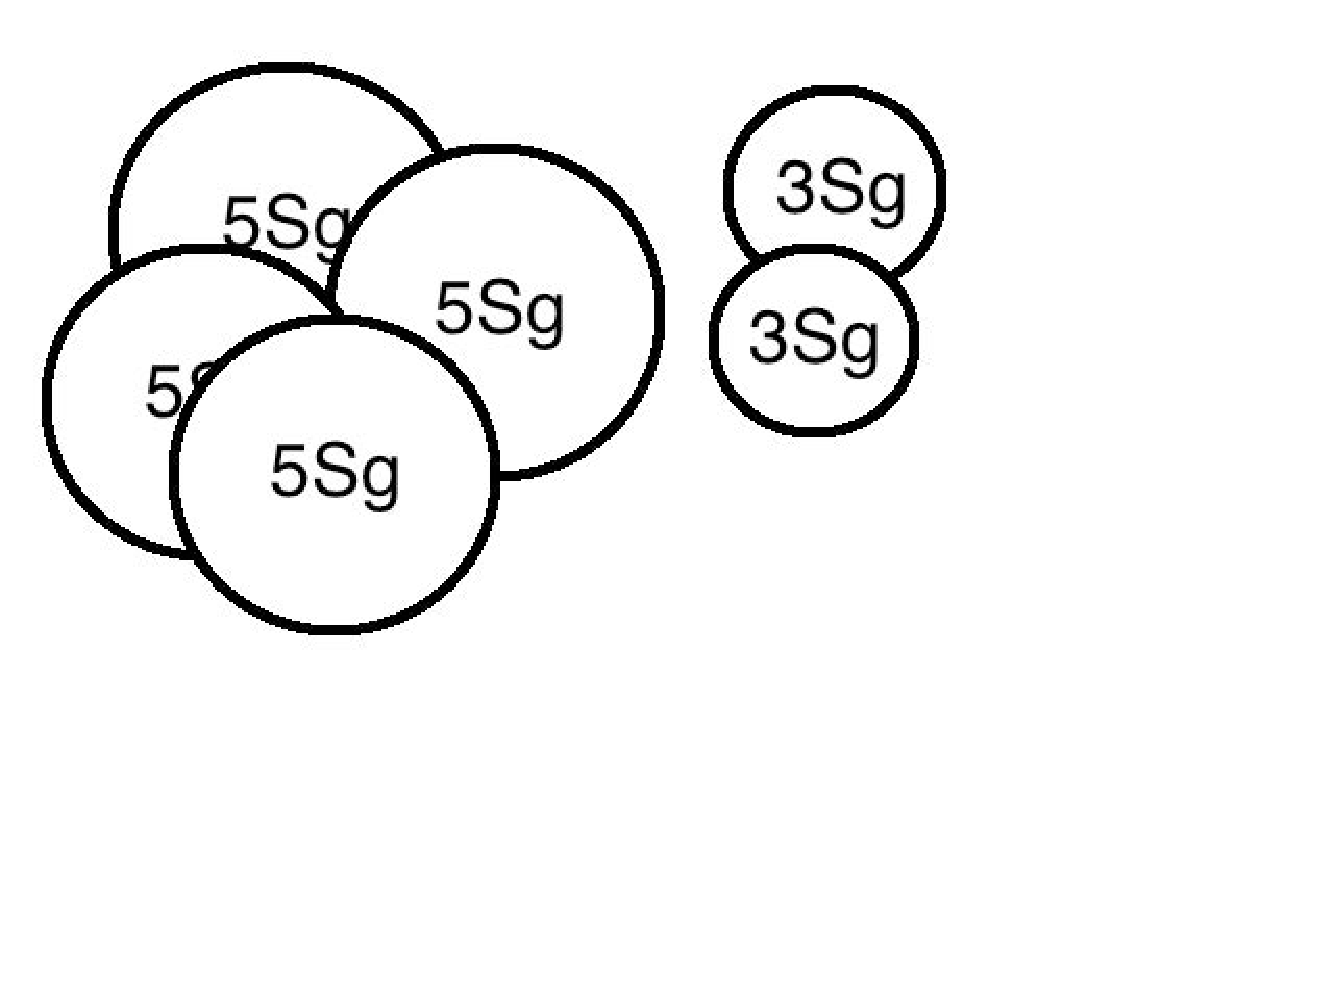
\includegraphics[trim = 0in 2.4in 2.5in 0in, clip, width = 3in]{Strong_Coins_image}
\caption{One way to make 26 Sg using Strongian currency}
\label{strong_coins}
\end{figure}

Strong induction makes this easy to prove for $n+1 \ge 11$, because then
$(n+1)-3 \ge 8$, so by strong induction the Inductians can make change for
exactly $(n+1)-3$ Strongs, and then they can add a 3\sg\ coin to get
$(n+1)\sg$.  So the only thing to do is check that they can make change
for all the amounts from 8 to 10\sg, which is not too hard to do.

Here's a detailed writeup using the official format:

\begin{proof}

  We prove by strong induction that the Inductians can make change for any
  amount of at least 8\sg.  The induction hypothesis, $P(n)$ will be:
\begin{quote}
There is a collection of coins whose value is $n+8$ Strongs.
\end{quote}

We now proceed with the induction proof:

\inductioncase{Base case}: $P(0)$ is true because a 3\sg\ coin together with
a 5\sg\ coin makes 8\sg.

\inductioncase{Inductive step}:  We assume $P(k)$ holds for all $k \leq n$, and
prove that $P(n+1)$ holds.  We argue by cases:

\textbf{Case} ($n+1$ = 1): We have to make $(n+1) +8 =9$\sg.  We can do this using three 3\sg\ coins.

\textbf{Case} ($n+1$ = 2): We have to make $(n+1) +8 =10$\sg.  Use two
5\sg\ coins.

\textbf{Case} ($n+1 \geq 3$): Then $0 \leq n - 2 \leq n$, so by the
strong induction hypothesis, the Inductians can make change for $n-2$
Strong.  Now by adding a 3\sg\ coin, they can make change for
$(n+1)\sg$.

Since $n \ge 0$, we know that $n + 1 \ge 1$ and thus that the three cases
cover every possibility.  Since $P(n+1)$ is true in every case, we can
conclude by strong induction
that for all $n \ge 0$, the Inductians can make change for $n+8$
Strong.  That is, they can make change for any number of eight or more
Strong.
\end{proof}

\subsection{The Stacking Game}

Here is another exciting game that's surely about to sweep the
nation!

%\hyperdef{stack}{game}
You begin with a stack of $n$ boxes.  Then you
make a sequence of moves.  In each move, you divide one stack of boxes
into two nonempty stacks.  The game ends when you have $n$ stacks, each
containing a single box.  You earn points for each move; in particular, if
you divide one stack of height $a + b$ into two stacks with heights $a$
and $b$, then you score $ab$ points for that move.  Your overall score is
the sum of the points that you earn for each move.  What strategy should
you use to maximize your total score?

As an example, suppose that we begin with a stack of $n = 10$ boxes.
Then the game might proceed as shown in Figure~\ref{fig:stacking-10}.
Can you find a better strategy?
%
\begin{figure}\redrawntrue
\[
\begin{array}{cccccccccccl}
\multicolumn{10}{c}{\textbf{Stack Heights}} & \quad & \textbf{Score} \\
\underline{10}&&&&&&&&& && \\
5&\underline{5}&&&&&&&& && 25 \text{ points} \\
\underline{5}&3&2&&&&&&& && 6 \\
\underline{4}&3&2&1&&&&&& && 4 \\
2&\underline{3}&2&1&2&&&&& && 4 \\
\underline{2}&2&2&1&2&1&&&& && 2 \\
1&\underline{2}&2&1&2&1&1&&& && 1 \\
1&1&\underline{2}&1&2&1&1&1&& && 1 \\
1&1&1&1&\underline{2}&1&1&1&1& && 1 \\
1&1&1&1&1&1&1&1&1&1 && 1 \\ \hline
\multicolumn{10}{r}{\textbf{Total Score}} & = & 45 \text{ points}
\end{array}
\]
\caption{An example of the stacking game with $n = 10$ boxes.  On each
line, the underlined stack is divided in the next step.}
\label{fig:stacking-10}
\end{figure}

\subsubsection{Analyzing the Game}

%Hide in full version
\iffalse
You will see in class how to use strong induction to analyze this game of
blocks.
\fi

%end Hide

%\iffalse  %unHide after Friday lecture:

Let's use strong induction to analyze the unstacking game.  We'll prove
that your score is determined entirely by the number of boxes---your
strategy is irrelevant!

\begin{theorem}\label{stacking}
Every way of unstacking $n$ blocks gives a score of $n(n-1)/2$ points.
\end{theorem}

There are a couple technical points to notice in the proof:

\begin{itemize}

\item The template for a strong induction proof mirrors the one for
  ordinary induction.

\item As with ordinary induction, we have some freedom to adjust indices.
In this case, we prove $P(1)$ in the base case and prove that $P(1),
\dots, P(n)$ imply $P(n+1)$ for all $n \geq 1$ in the inductive step.

\end{itemize}

\begin{proof}
The proof is by strong induction.  Let $P(n)$ be the proposition that
every way of unstacking $n$ blocks gives a score of $n(n-1)/2$.

\inductioncase{Base case}: If $n = 1$, then there is only one
block.  No moves are possible, and so the total score for the game is
$1(1 - 1)/2 = 0$.  Therefore, $P(1)$ is true.

\inductioncase{Inductive step}: Now we must show that $P(1)$, \dots, $P(n)$ imply
$P(n+1)$ for all $n \geq 1$.  So assume that $P(1)$, \dots, $P(n)$ are all
true and that we have a stack of $n+1$ blocks.  The first move must split
this stack into substacks with positive sizes $a$ and $b$ where $a+b =
n+1$ and $0<a,b\leq n$.  Now the total score for the game is the sum of
points for this first move plus points obtained by unstacking the two
resulting substacks:
%
\begin{align*}
\text{total score}
    & = \text{(score for 1st move)} \\
    & \quad + \text{(score for unstacking $a$ blocks)} \\
    & \quad + \text{(score for unstacking $b$ blocks)} \\
    & = ab + \frac{a(a-1)}{2} + \frac{b(b-1)}{2} & \text{by $P(a)$ and $P(b)$}\\
    & = \frac{(a+b)^2-(a+b)}{2} = \frac{(a+b)((a+b)-1)}{2}\\
    & = \frac{(n+1)n}{2}
\end{align*}
%
This shows that $P(1)$, $P(2)$, \dots, $P(n)$ imply $P(n+1)$.

Therefore, the claim is true by strong induction.
\end{proof}

%\fi
%end unHide

%% Strong Induction Problems %%%%%%%%%%%%%%%%%%%%%%%%%%%%%%%%%%%%%%%%%%%%%%%%%%

\begin{problems}
\practiceproblems
\pinput{TP_Induction_Rules}
\pinput{TP_a_bogus_fibonacci_induction}
\pinput{TP_another_bogus_fibonacci_induction}
\pinput{TP_Induction_by_n+3}

\classproblems
\pinput{CP_fibonacci_by_induction}
\pinput{CP_bogus_unique_prime_factors}
\pinput{CP_box_unstacking} %not strong induction, but depends on stacking game

\homeworkproblems
\pinput{PS_team_division}
\pinput{PS_bogus_prime_divides_integer_product}

\examproblems
\pinput{MQ_fib_squares}
\pinput{FP_3_exponent_inequality_induction}
\pinput{FP_4_and_7_cent_stamps_by_induction}
\pinput{MQ_10_and_15_cents_induction}

\end{problems}

\section{Strong Induction vs.\ Induction vs.\ Well Ordering}
\label{versusWO}

Strong induction looks genuinely ``stronger'' than ordinary induction
---after all, you can assume a lot more when proving the induction
step.  Since ordinary induction is a special case of strong induction,
you might wonder why anyone would bother with the ordinary induction.

But strong induction really isn't any stronger, because a simple text
manipulation program can automatically reformat any proof using strong
induction into a proof using ordinary induction---just by decorating the
induction hypothesis with a universal quantifier in a standard way.
Still, it's worth distinguishing these two kinds of induction, since which
you use will signal whether the inductive step for $n+1$ follows directly
from the case for $n$ or requires cases smaller than $n$, and that is
generally good for your reader to know.

The template for the two kinds of induction rules looks nothing like
the one for the \idx{Well Ordering Principle}, but this chapter
included a couple of examples where induction was used to prove
something already proved using Well Ordering.  In fact, this can
always be done.  As the examples may suggest, any Well Ordering proof
can automatically be reformatted into an Induction proof.  So
theoretically, no one need bother with the Well Ordering Principle
either.

But wait a minute!  It's equally easy to go the other way, and
automatically reformat any Strong Induction proof into a Well Ordering
proof.  The three proof methods---Well Ordering, Induction, and Strong
Induction---are simply different formats for presenting the same
mathematical reasoning!

So why three methods?  Well, sometimes induction proofs are clearer
because they don't require proof by contradiction.  Also, induction
proofs often provide recursive procedures that reduce large inputs to
smaller ones.  On the other hand, Well Ordering can come out slightly
shorter and sometimes seem more natural, and less worrisome to
beginners.

So which method should you use?  There is no simple recipe.  Sometimes
the only way to decide is to write up a proof using more than one
method and compare how they come out.  But whichever method you
choose, be sure to state the method up front to help a reader follow
your proof.

\begin{editingnotes}
Here's how to reformat an induction proof and into a Well
Ordering proof : suppose that we have a proof by induction with
hypothesis $P(n)$.  Then we start a Well Ordering proof by assuming the
set of counterexamples to $P$ is nonempty.  Then by Well Ordering there is
a smallest counterexample, $s$, that is, a smallest $s$ such that $P(s)$
is false.

Now we use the proof of $P(0)$ that was part of the Induction proof to
conclude that $s$ must be greater than 0.  Also since $s$ is the smallest
counterexample, we can conclude that $P(s-1)$ must be true.  At this point
we reuse the proof of the inductive step in the Induction proof, which
shows that since $P(s-1)$ true, then $P(s)$ is also true.  This
contradicts the assumption that $P(s)$ is false, so we have the
contradiction needed to complete the Well Ordering Proof that $P(n)$ holds
for all $n \in \naturals$.

\end{editingnotes}


%%%%%%%FTL
\section{State Machines}\label{state_machine_sec}
State machines are a simple, abstract model of step-by-step processes.
Since computer programs can be understood as defining step-by-step
computational processes, it's not surprising that state machines come
up regularly in computer science.  They also come up in many other
settings such as designing digital circuits and modeling probabilistic
processes.  This section introduces \term{Floyd's Invariant Principle}
which is a version of induction tailored specifically for proving
properties of state machines.

\iffalse
You may already have seen them in a digital logic course,
a compiler course, or a probability course.
\fi

One of the most important uses of induction in computer science
involves proving one or more desirable properties continues to hold at
every step in a process.  A property that is preserved through a
series of operations or steps is known as an \term{invariant}.
Examples of desirable invariants include properties such as a variable
never exceeding a certain value, the altitude of a plane never
dropping below 1,000 feet without the wingflaps
\iffalse and landing gear\fi
being deployed, and the temperature of a nuclear reactor never
exceeding the threshold for a meltdown.

\iffalse  %%FTL
In particular, we show that the proposition is true at the beginning
(this is the base case) and that if it is true after $t$ steps have
been taken, it will also be true after step~$t + 1$ (this is the
inductive step).  We can then use the induction principle to conclude
that the proposition is indeed an invariant, namely, that it will
always hold.
\fi

\subsection{States and Transitions}

Formally, a state machine is nothing more than a binary relation on a
set, except that the elements of the set are called ``states,'' the
relation is called the \term{transition relation}, and an arrow in the
graph of the transition relation is called a \term{transition}.  A
transition from state $q$ to state $r$ will be written $q \movesto r$.
The transition relation is also called the \term{state graph} of the
machine.  A state machine also comes equipped with a designated
\emph{start state}.

A simple example is a bounded counter, which counts from $0$ to $99$
and overflows at 100.  This state machine is pictured in
Figure~\ref{fig:counter}, with states pictured as circles, transitions
by arrows, and with start state 0 indicated by the double circle.
\begin{figure}
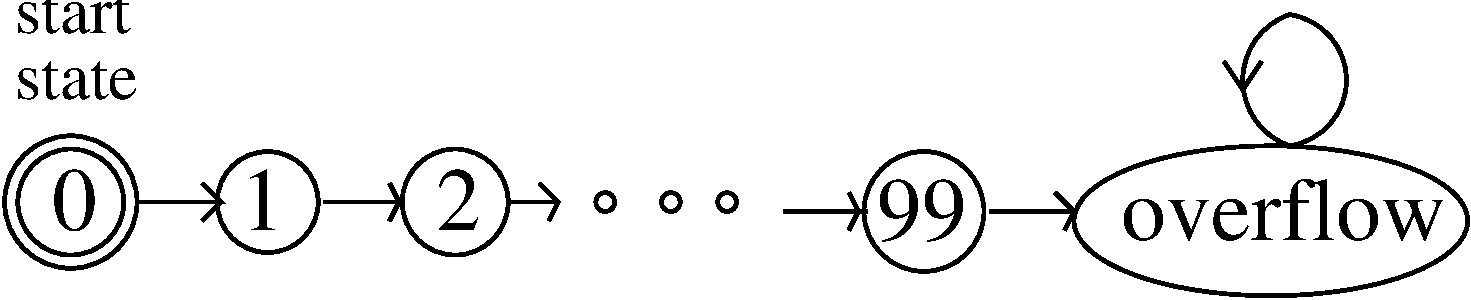
\includegraphics[width = 3in]{counter}
\caption{\em State transitions for the 99-bounded counter.}
\label{fig:counter}
\end{figure}
To be precise, what the picture tells us is that this bounded counter machine has
\begin{align*}
\text{states} &  \eqdef \set{0, 1,\dots,99, \text{overflow}},\\
\text{start state}  & \eqdef 0,\\
\text{transitions} & \eqdef \set{n \movesto n+1 \suchthat 0 \le n < 99}\\
                   &\quad  \union \set{99 \movesto \text{overflow},
                                 \text{overflow} \movesto \text{overflow}}.
\end{align*}
This machine isn't much use once it overflows, since it has no way to
get out of its overflow state.

State machines for digital circuits and string pattern matching
algorithms, for instance, usually have only a finite number of states.
Machines that model continuing computations typically have an infinite
number of states.  For example, instead of the 99-bounded counter, we
could easily define an ``unbounded'' counter that just keeps counting
up without overflowing.  The unbounded counter has an infinite state
set, the nonnegative integers, which makes its state diagram
harder to draw.

State machines are often defined with labels on states and/or transitions
to indicate such things as input or output values, costs, capacities, or
probabilities.  Our state machines don't include any such labels because
they aren't needed for our purposes.  We do name states, as in
Figure~\ref{fig:counter}, so we can talk about them, but the names aren't
part of the state machine.

\subsection{Invariant for a Diagonally-Moving Robot}
Suppose we have a robot that starts at the origin and moves on an
infinite 2-dimensional integer grid.  The \emph{state} of the robot at
any time can be specified by the integer coordinates $(x, y)$ of the
robot's current position.  So the \emph{start state} is~$(0, 0)$.  At
each step, the robot may move to a diagonally adjacent grid point, as
illustrated in Figure~\ref{fig:diagrobot}.

\begin{figure}
\graphic{Fig_robot-a}
\caption{\em The Diagonally Moving Robot.}
\label{fig:diagrobot}
\end{figure}

To be precise, the robot's transitions are:
\[
\set{(m,n)\movesto (m\pm 1, n\pm 1) \suchthat m,n \in \integers}.
\]
For example, after the first step, the robot could be in states $(1,
1)$, $(1, -1)$, $(-1, 1)$, or $(-1, -1)$.  After two steps, there are
9 possible states for the robot, including~$(0, 0)$.
The question is, can the robot ever reach position~$(1, 0)$?

\begin{figure}
\graphic{Fig_robot-b}
\caption{\em Can the Robot get to $(1,0)$?}
\label{fig:robot-to10}
\end{figure}

If you play around with the robot a bit, you'll probably notice that
the robot can only reach positions~$(m, n)$ for which $m + n$ is even,
which of course means that it can't reach $(1,0)$.  This follows
because the evenness of the sum of the coordinates is preserved by
transitions.

This once, let's go through this preserved-property argument,
carefully highlighting where induction comes in.  Specifically, define the
even-sum property of states to be:
\[
\text{Even-sum}((m,n)) \eqdef [m+n \text{ is even}].
\]
\begin{lemma}\label{even-sum-invar}
For any transition, $q \movesto r$, of the diagonally-moving robot, if
Even-sum($q$), then Even-sum($r$).
\end{lemma}
This lemma follows immediately from the definition of the robot's
transitions: $(m,n)\movesto (m\pm 1, n\pm 1)$.  After a transition,
the sum of coordinates changes by $(\pm 1) + (\pm 1)$, that is, by 0,
2, or -2.  Of course, adding 0, 2 or -2 to an even number gives an
even number.  So by a trivial induction on the number of transitions,
we can prove:
\begin{theorem}\label{th:diag-robot}
The sum of the coordinates of any state reachable by the
diagonally-moving robot is even.
\end{theorem}

\begin{proof}
The proof is induction on the number of transitions the robot has
made.  The induction hypothesis is
\[
P(n) \eqdef \text{if $q$ is a state reachable in $n$ transitions, then
  Even-sum($q$)}.
\]

\inductioncase{base case}: $P(0)$ is true since the only state reachable in 0
transitions is the start state $(0, 0)$, and $0 + 0$ is even.

\inductioncase{inductive step}: Assume that $P(n)$ is true, and let $r$ be any
state reachable in $n+1$ transitions. We need to prove that
Even-sum($r$) holds.

Since $r$ is reachable in $n+1$ transitions, there must be a state,
$q$, reachable in $n$ transitions such that $q \movesto r$.  Since
$P(n)$ is assumed to be true, Even-sum($q$) holds, and so by
Lemma~\ref{even-sum-invar}, Even-sum($r$) also holds.  This proves
that $P(n) \QIMPLIES P(n + 1)$ as required, completing the proof of
the inductive step.

We conclude by induction that for all $n \ge 0$, if $q$ is reachable
in $n$ transitions, then Even-sum($q$).  This implies that every
reachable state has the Even-sum property.

\end{proof}

\begin{corollary}\label{cor:diag-robot}
The robot can never reach position~$(1, 0)$.
\end{corollary}

\begin{proof}
By Theorem~\ref{th:diag-robot}, we know the robot can only reach
positions with coordinates that sum to an even number, and thus it
cannot reach position~$(1, 0)$.
\end{proof}

\iffalse
Since this was the first time we proved that a predicate was an
invariant, we were careful to go through all four cases in gory
detail.  As you become more experienced with such proofs, you will
likely become more brief as well.  Indeed, if we were going through
the proof again at a later point in the text, we might simply note
that the sum of the coordinates after step~$t + 1$ can be only $x +
y$, $x + y + 2$ or $x + y - 2$ and therefore that the sum is even.
%%%%%%%%%%%%FTL
\fi

\subsection{The Invariant Principle}
Using the Even-sum invariant to understand the diagonally-moving robot
is a simple example of a basic proof method called The Invariant
Principle.  The Principle summarizes how induction on the number of
steps to reach a state applies to invariants.   

\iffalse

To formulate it precisely, we need a definition of
\term{reachability.}

\begin{definition}
The \term{reachable states} of a state machine, $M$, are defined
recursively as follows:
\begin{itemize}
\item the start state is reachable, and
\item if $p$ is a reachable state of $M$, and $p \movesto q$ is a
  transition of $M$, then $q$ is also a reachable state of $M$.
\end{itemize}
\end{definition}
\fi

A state machine \emph{execution} describes a possible sequence of
steps a machine might take.

\begin{definition}
An \term{execution} of the state machine is a (possibly infinite)
sequence of states with the property that
\begin{itemize}
\item it begins with the start state, and
\item if $q$ and $r$ are consecutive states in the sequence, the $q \movesto r$.
\end{itemize}
A state is called \term{reachable} if it appears in some execution.
\end{definition}

\begin{definition}
  A \term{preserved invariant} of a state machine is a predicate, $P$, on
  states, such that whenever $P(q)$ is true of a state, $q$, and $q
  \movesto r$ for some state, $r$, then $P(r)$ holds.
\end{definition}

\textbox{
\textboxheader{The Invariant Principle}

\noindent If a preserved invariant of a state machine is true for the
start state,\\
then it is true for all reachable states.}

The Invariant Principle is nothing more than the Induction Principle
reformulated in a convenient form for state machines.  Showing that a
predicate is true in the start state is the base case of the induction,
and showing that a predicate is a preserved invariant corresponds to the
inductive step.\footnote{Preserved invariants are commonly just called
  ``invariants'' in the literature on program correctness, but we decided
  to throw in the extra adjective to avoid confusion with other
  definitions.  For example, other texts (as well as another subject at
  MIT) use ``invariant'' to mean ``predicate true of all reachable
  states.''  Let's call this definition ``invariant-2.''  Now invariant-2
  seems like a reasonable definition, since unreachable states by
  definition don't matter, and all we want to show is that a desired
  property is invariant-2.  But this confuses the \emph{objective} of
  demonstrating that a property is invariant-2 with the \emph{method} of
  finding a \emph{preserved} invariant to \emph{show} that it is
  invariant-2.}

\textbox{
\textboxheader{Robert W Floyd}
\begin{center}
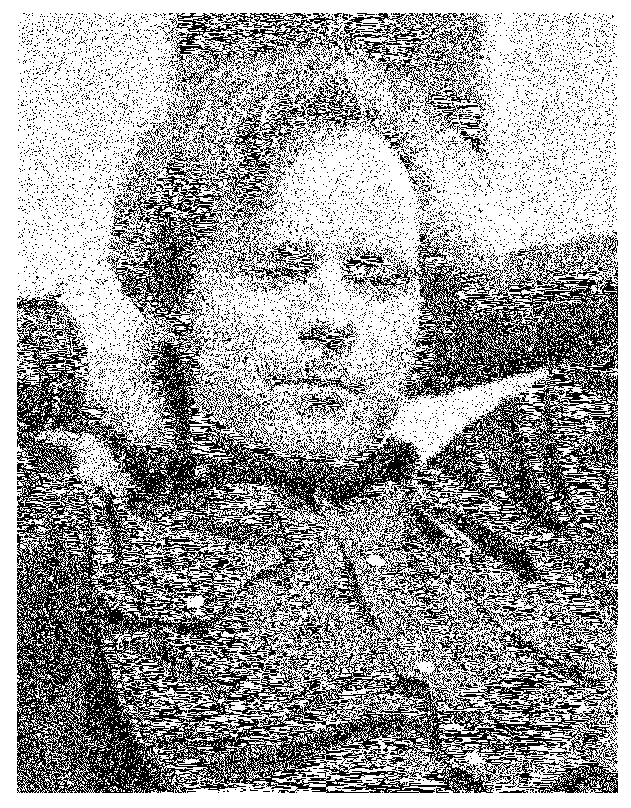
\includegraphics[width = 2in]{floyd72}
\end{center}

The Invariant Principle was formulated by Robert W. Floyd at Carnegie
Tech in 1967. (The following year, Carnegie Tech was renamed
Carnegie-Mellon University)  Floyd was already famous for work on the formal
grammars that transformed the field of programming language parsing;
that was how he got to be a professor even though he never got a Ph.D.
(He was admitted to a PhD program as a teenage prodigy, but flunked
out and never went back.)

In that same year, Albert R. Meyer was appointed Assistant Professor in
the Carnegie Tech Computer Science Department, where he first met Floyd.
Floyd and Meyer were the only theoreticians in the department, and they
were both delighted to talk about their shared interests.  After just a
few conversations, Floyd's new junior colleague decided that Floyd was the
smartest person he had ever met.

Naturally, one of the first things Floyd wanted to tell Meyer about was
his new, as yet unpublished, Invariant Principle.  Floyd explained the
result to Meyer, and Meyer wondered (privately) how someone as brilliant
as Floyd could be excited by such a trivial observation.  Floyd had to
show Meyer a bunch of examples before Meyer understood Floyd's excitement
---not at the truth of the utterly obvious Invariant Principle, but rather
at the insight that such a simple method could be so widely and easily
applied in verifying programs.

Floyd left for Stanford the following year.  He won the Turing award,
the ``Nobel prize'' of computer science, in the late 1970's, in
recognition of his work on grammars and on the foundations of
program verification.  He remained at Stanford from 1968 until his
death in September, 2001.  You can learn more about Floyd's life and
work by reading the
\href{http://courses.csail.mit.edu/6.042/spring11/floyd-eulogy-by-knuth.pdf}{eulogy}
at
\begin{center}
http://oldwww.acm.org/pubs/membernet/stories/floyd.pdf
\end{center}
written by his closest colleague, Don Knuth.

 \iffalse
   \href{http://oldwww.acm.org/pubs/membernet/stories/floyd.pdf}
{\texttt{http://oldwww.acm.org/pubs/membernet/stories/floyd.pdf}}.
\fi
}

\subsection{The Die Hard Example}\label{diehard_example}
The movie \textit{Die Hard 3: With a Vengeance} includes an amusing
example of a state machine.  The lead characters played by Samuel
L. Jackson and Bruce Willis have to disarm a bomb planted by the
diabolical Simon Gruber:

\textbox{
\begin{list}{}{\itemsep=0in \leftmargin=0.25in \rightmargin=0.25in}

\item[\textbf{Simon:}] On the fountain, there should be 2 jugs, do you
see them?  A 5-gallon and a 3-gallon.  Fill one of the jugs with
exactly 4 gallons of water and place it on the scale and the timer
will stop.  You must be precise; one ounce more or less will result in
detonation.  If you're still alive in 5 minutes, we'll speak.

\item[\textbf{Bruce:}] Wait, wait a second. I don't get it. Do you get it?

\item[\textbf{Samuel:}] No.

\item[\textbf{Bruce:}] Get the jugs. Obviously, we can't fill the 3-gallon jug
with 4 gallons of water.

\item[\textbf{Samuel:}] Obviously.

\item[\textbf{Bruce:}] All right. I know, here we go. We fill the 3-gallon jug
exactly to the top, right?

\item[\textbf{Samuel:}] Uh-huh.

\item[\textbf{Bruce:}] Okay, now we pour this 3 gallons into the 5-gallon jug,
giving us exactly 3 gallons in the 5-gallon jug, right?

\item[\textbf{Samuel:}] Right, then what?

\item[\textbf{Bruce:}] All right. We take the 3-gallon jug and fill it a third
of the way...

\item[\textbf{Samuel:}] No!  He said, ``Be precise.''  Exactly 4
gallons.

\item[\textbf{Bruce:}] Sh - -.  Every cop within 50 miles is running his a - - off
and I'm out here playing kids games in the park.

\item[\textbf{Samuel:}] Hey, you want to focus on the problem at hand?

\end{list}
}

Fortunately, they find a solution in the nick of time.  You can work out
how.

\subsubsection{The Die Hard 3 State Machine}\label{diehard_machine}
The jug-filling scenario can be modeled with a state machine that keeps
track of the amount, $b$, of water in the big jug, and the amount, $l$,
in the little jug.  With the 3 and 5 gallon water jugs, the states
formally will be pairs, $(b,l)$, of real numbers such that $0 \leq b \leq
5, 0 \leq l \leq 3$.  (We can prove that the reachable values of $b$ and
$l$ will be nonnegative integers, but we won't assume this.)  The start
state is $(0,0)$, since both jugs start empty.

Since the amount of water in the jug must be known exactly, we will only
consider moves in which a jug gets completely filled or completely
emptied.  There are several kinds of transitions:
\begin{enumerate}

\item  Fill the little jug: $(b,l) \movesto (b,3)$ for $l < 3$.

\item  Fill the big jug: $(b,l) \movesto (5,l)$ for $b<5$.

\item  Empty the little jug: $(b,l) \movesto (b,0)$ for $l>0$.

\item  Empty the big jug: $(b,l) \movesto (0,l)$ for $b>0$.

\item  Pour from the little jug into the big jug: for $l>0$,
\begin{equation*}
(b,l) \movesto
\begin{cases}
(b+l, 0) & \text{if $b + l \le 5$,}\\
(5, l - (5 - b)) & \text{otherwise.}
\end{cases}
\end{equation*}

\item Pour from big jug into little jug: for $b>0$,
\begin{equation*}
(b,l) \movesto
\begin{cases}
(0, b+l) & \text{if $b + l \le 3$,}\\
(b - (3 -l), 3) & \text{otherwise.}
\end{cases}
\end{equation*}
\end{enumerate}

Note that in contrast to the 99-counter state machine, there is more than
one possible transition out of states in the Die Hard machine.  Machines
like the 99-counter with at most one transition out of each state are
called \emph{deterministic}.  The Die Hard machine is
\emph{nondeterministic} because some states have transitions to several
different states.

The Die Hard 3 bomb gets disarmed successfully because the state (4,3)
is reachable.

%\end{example}

%\subsubsection{Reachability and Preserved Invariants}

\subsubsection{Die Hard Once and For All}
The \emph{Die Hard} series is getting tired, so we propose a final
\emph{Die Hard Once and For All}.  Here, Simon's brother returns to
avenge him, posing the same challenge, but with the 5 gallon jug
replaced by a 9 gallon one.  The state machine has the same
specification as the Die Hard 3 version, except all occurrences of
``5'' are replaced by ``9.''

Now, reaching any state of the form $(4,l)$ is impossible.  We prove
this using the Invariant Principle.  Specifically, we define the
preserved invariant predicate, $P((b,l))$, to be that $b$ and $l$ are
nonnegative integer multiples of 3.

To prove that $P$ is a preserved invariant of Die-Hard-Once-and-For-All
machine, we assume $P(q)$ holds for some state $q \eqdef (b,l)$ and that
$q \movesto r$.  We have to show that $P(r)$ holds.  The proof divides
into cases, according to which transition rule is used.

One case is a ``fill the little jug'' transition.  This means $r =
(b,3)$.  But $P(q)$ implies that $b$ is an integer multiple of 3, and
of course 3 is an integer multiple of 3, so $P(r)$ still holds.

Another case is a ``pour from big jug into little jug'' transition.
For the subcase when there isn't enough room in the little jug to hold
all the water, that is, when $b + l > 3$, we have $r = (b -( 3 -l), 3)$.
But $P(q)$ implies that $b$ and $l$ are integer multiples of 3, which
means $b -( 3 -l)$ is too, so in this case too, $P(r)$ holds.

We won't bother to crank out the remaining cases, which can all be checked
just as easily.  Now by the Invariant Principle, we conclude that every
reachable state satisifies $P$.  But since no state of the form $(4,l)$
satisifies $P$, we have proved rigorously that Bruce dies once and for
all!

By the way, notice that the state (1,0), which satisfies $\QNOT(P)$, has a
transition to (0,0), which satisfies $P$.  So the negation of a preserved
invariant may not be a preserved invariant.

\subsection{Fast Exponentiation}\label{fast_exp_subsec}

\subsubsection{Partial Correctness \& Termination}

Floyd distinguished two required properties to verify a program.  The
first property is called \term{partial correctness}; this is the property
that the final results, if any, of the process must satisfy system
requirements.

You might suppose that if a result was only partially correct, then it
might also be partially incorrect, but that's not what Floyd meant.  The
word ``partial'' comes from viewing a process that might not terminate as
computing a \emph{partial relation}.  Partial correctness means that
\emph{when there is a result}, it is correct, but the process might not
always produce a result, perhaps because it gets stuck in a loop.

The second correctness property, called \emph{termination}, is that the
process does always produce some final value.

Partial correctness can commonly be proved using the Invariant Principle.
Termination can commonly be proved using the Well Ordering Principle.
We'll illustrate this by verifying a Fast Exponentiation procedure.

\subsubsection{Exponentiating}\label{fast_exp_subsubsec}
The most straightforward way to compute the $b$th power of a number,
$a$, is to multiply $a$ by itself $b-1$ times.  But the solution can
be found in considerably fewer multiplications by using a technique
called \term{Fast Exponentiation}.  The register machine program below
defines the fast exponentiation algorithm.  The letters $x,y,z,r$
denote registers that hold numbers. An \term{assignment statement} has
the form ``$z := a$'' and has the effect of setting the number in
register $z$ to be the number $a$.

\textbox{
\textboxheader{A Fast Exponentiation Program}

Given inputs $a \in \reals, b \in \naturals$,
initialize registers $x,y,z$ to $a,1,b$ respectively,
and repeat the following sequence of steps until termination:
\begin{itemize}\renewcommand{\itemsep}{0pt}
\item if $z = 0$ \textbf{return} $y$ and terminate
\item $r := \text{remainder}(z,2)$
\item $z := \quotient(z,2)$
\item if $r = 1$, then $y := xy$
\item $x := x^2$
\end{itemize}
}

We claim this program always terminates and leaves $y = a^b$.

To begin, we'll model the behavior of the program with a state
machine:
\begin{enumerate}
\item $\text{states} \eqdef \reals \cross \reals \cross \naturals$,
\item $\text{start state} \eqdef (a,1,b)$,
\item transitions are defined by the rule
\begin{equation*}
(x,y,z) \movesto
\begin{cases}
(x^2, y, \quotient(z,2)) & \text{if $z$ is nonzero and even},\\
(x^2, xy, \quotient(z,2)) & \text{if $z$ is nonzero and odd}.
\end{cases}
\end{equation*}
\end{enumerate}

The preserved invariant, $P((x,y,z))$, will be
\begin{equation}\label{yxzd}
z \in \naturals \QAND yx^z = a^b.
\end{equation}

To prove that $P$ is preserved, assume $P((x,y,z))$ holds
and that $(x,y,z) \movesto (x_t,y_t,z_t)$.  We must prove that
$P((x_t,y_t,z_t))$ holds, that is,
\begin{equation}\label{ztytxt}
z_t \in \naturals \QAND y_tx_t^{z_t} = a^b.
\end{equation}

Since there is a transition from $(x,y,z)$, we have $z \neq 0$, and since
$z \in \naturals$ by~\eqref{yxzd}, we can consider just two cases:

If $z$ is even, then we have that $x_t = x^2, y_t = y, z_t = z/2$.
Therefore, $z_t \in \naturals$ and
\begin{align*}
y_tx_t^{z_t} & = y(x^2)^{z/2}\\
           & = yx^{2\cdot z/2}\\
           & = yx^z\\
           & = a^b & \mbox{(by~\eqref{yxzd})}
\end{align*}

If $z$ is odd, then we have that $x_t = x^2, y_t = xy, z_t = (z-1)/2$.
Therefore, $z_t \in \naturals$ and
\begin{align*}
y_tx_t^{z_t} & = xy(x^2)^{(z-1)/2}\\
& = yx^{1+2 \cdot (z-1)/2}\\
& = yx^{1+(z-1)}\\
& = yx^z\\
& = a^b & \mbox{(by~\eqref{yxzd})}
\end{align*}

So in both cases,~\eqref{ztytxt} holds, proving that $P$ is a preserved
invariant.

Now it's easy to prove partial correctness: if the Fast
Exponentiation program terminates, it does so with $a^b$ in register
$y$.  This works because obviously $1\cdot a^b = a^b$, which means
that the start state, $(a,1,b)$, satisifies $P$.  By the Invariant
Principle, $P$ holds for all reachable states.  But the program
only stops when $z = 0$.  If a terminated state $(x,y,0)$ is
reachable, then $y = yx^0 = a^b$ as required.

Ok, it's partially correct, but what's fast about it?  The answer is
that the number of multiplications it performs to compute $a^b$ is
roughly the length of the binary representation of $b$.  That is, the
Fast Exponentiation program uses roughly $\log_2 b$ multiplications,
compared to the naive approach of multiplying by $a$ a total of $b-1$
times.

More precisely, it requires at most $2 (\ceil{\log_2 b}+1)$
multiplications for the Fast Exponentiation algorithm to compute $a^b$ for
$b>1$.  The reason is that the number in register $z$ is initially $b$,
and gets at least halved with each transition.  So it can't be halved more
than $\ceil{\log_2 b}+1$ times before hitting zero and causing the
program to terminate.  \iffalse The $(b+1)$ comes in because for $b =
2^p$, a power of two, it takes $(p+1)$ halves to get zero.  \fi Since each
of the transitions involves at most two multiplications, the total number
of multiplications until $z=0$ is at most $2(\ceil{\log_2 b}+1)$ for $b
> 0$ (see Problem~\ref{PS_2logb_mults}).

\subsection{Derived Variables}\label{derived_var_subsec}

The preceding termination proof involved finding a nonnegative
integer-valued measure to assign to states.  We might call this measure
the ``size'' of the state.  We then showed that the size of a state
decreased with every state transition.  By the Well Ordering Principle,
the size can't decrease indefinitely, so when a minimum size state is
reached, there can't be any transitions possible: the process has
terminated.

More generally, the technique of assigning values to states---not
necessarily nonnegative integers and not necessarily decreasing under
transitions---is often useful in the analysis of algorithms.
\emph{Potential functions} play a similar role in physics.  In the
context of computational processes, such value assignments for states
are called \term{derived variables}.

For example, for the Die Hard machines we could have introduced a derived
variable, $f:\text{states} \to \reals$, for the amount of water in both
buckets, by setting $f((a, b)) \eqdef a + b$.  Similarly, in the robot
problem, the position of the robot along the $x$-axis would be given by
the derived variable $x\text{-coord}$, where $x\text{-coord}((i, j))
\eqdef~i$.

%\subsubsection{Weakly Decreasing Variables}

There are a few standard properties of derived variables that are handy in
analyzing state machines.

\begin{definition}
  A derived variable $f:\text{states} \to \reals$ is \term{strictly
    decreasing} iff
\[
q \movesto q' \QIMP\ f(q') < f(q).
\]
It is \term{weakly decreasing} iff
\[
q \movesto q' \QIMP\ f(q') \leq f(q).
\]

\term{Strictly increasing} and \term{weakly increasing} derived
variables are defined similarly.\footnote{Weakly increasing variables
  are often also called \emph{nondecreasing}.  We will avoid this
  terminology to prevent confusion between nondecreasing variables and
  variables with the much weaker property of \emph{not} being a
  decreasing variable.}
\end{definition}

We confirmed termination of the Fast Exponentiation procedure by
noticing that the derived variable $z$ was nonnegative-integer-valued
and strictly decreasing.  We can summarize this approach to proving
termination as follows:
\begin{theorem}\label{th:decr}
If $f$ is a strictly decreasing $\naturals$-valued derived variable of a
state machine, then the length of any execution starting at state $q$ is
at most $f(q)$.
\end{theorem}

Of course, we could prove Theorem~\ref{th:decr} by induction on the value
of $f(q)$, but think about what it says: ``If you start counting down at
some nonnegative integer $f(q)$, then you can't count down more than
$f(q)$ times.''  Put this way, it's obvious.

Theorem~\ref{th:decr} generalizes straightforwardly to derived
variables taking values in a well ordered set.

\begin{theorem}\label{well_order_decreasing}
  If there exists a strictly decreasing derived variable whose range
  is a well ordered set, then every execution terminates.
\end{theorem}

Theorem~\ref{well_order_decreasing} follows immediately from the
observation that a set of numbers is well ordered iff it has no
infinite decreasing sequences
(Problem~\ref{CP_well_order_decreasing}).

Note that the existence of a \emph{weakly} decreasing derived variable
does not guarantee that every execution terminates.  An
infinite execution could proceed through states in which a weakly
decreasing variable remained constant.

\subsubsection{A Southeast Jumping Robot (Optional)}

\iffalse Begin by defining the trivial ``pick how long'' game: P1 picks $n
\in \naturals$, the P2 and P1 alternate making forced moves.  The game
ends after $n$ forced moves; the last person to move wins.  So P1 strategy
is ``pick and even number.''  Insert here the discussion of ``terminates,
but no bound on number of steps...'' used below.

May also tell the ``guess a bigger number game''joke.
\fi

Here's a contrived, simple example of proving termination based on a
variable that is strictly decreasing over a well ordered set.  Let's
think about a robot positioned at an integer lattice-point in the
Northeast quadrant of the plane, that is, at $(x,y) \in \naturals^2$.

At every second when it is away from the origin, $(0,0)$, the robot must
make a move, which may be
\begin{itemize}

\item a unit distance West when it is not at the boundary of the Northeast
  quadrant (that is, $(x,y) \movesto (x-1,y)$ for $x>0$), or

\item a unit distance South combined with an arbitrary jump East (that is,
     $(x,y) \movesto (z,y-1)$ for $z\geq x$).

\end{itemize}
\begin{claim}\label{robotcl}
The robot will always get stuck at the origin.
\end{claim}

If we think of the robot as a nondeterministic state machine, then
Claim~\ref{robotcl} is a termination assertion.  The Claim may seem
obvious, but it really has a different character than termination based on
nonnegative integer-valued variables.  That's because, even knowing that
the robot is at position $(0,1)$, for example, there is no way to bound
the time it takes for the robot to get stuck.  It can delay getting stuck
for as many seconds as it wants by making its next move to a distant point
in the Far East.  This rules out proving termination using
Theorem~\ref{th:decr}.

So does Claim~\ref{robotcl} still seem obvious?

Well it is if you see the trick.  Define a derived variable, $v$, mapping
robot states to the numbers in the well ordered set $\naturals + \twdone$
of Lemma~\ref{to1_well-order}.  In particular, define
$v:\naturals^2 \to \naturals + \twdone$ as follows
\[
v(x,y) \eqdef y + \frac{x}{x+1}.
\]

Now it's easy to check that if $(x,y)\movesto (x',y')$ is a legitimate
robot move, then $v((x',y')) < v((x,y))$.  In particular, $v$ is a
strictly decreasing derived variable, so
Theorem~\ref{well_order_decreasing} implies that the robot always get
stuck---even though we can't say how many moves it will take until it
does.

\iffalse

We will prove that the robot always gets stuck at the origin by
generalizing the decreasing variable method, but with decreasing values
that are more general than nonnegative integers.  Namely, the traveling robot
can be modeled with a state machine with states of the form $((x,y),s,e)$
where
\begin{itemize}
\item $(x,y) \in \naturals^2$ is the robot's position,
\item $s$ is the number of moves South the robot took to get to this
position, and
\item $e \le 2s$ is the number of moves East the robot took to get to this
position. 
\end{itemize}

Now we define a derived variable $\vl:\text{States}\to \naturals^3$:
\[
\vl(((x,y),s,e)) \ \eqdef\quad (y,2s-e,x),
\]
and we order the values of states with the \emph{lexicographic} order,
$\lexle$, on $\naturals^3$:
\begin{equation}\label{lex3}
(k,l,m) \lexle (k',l',m') \ \eqdef\quad k < k' \text{ or } (k=k' \text{
and } l < l') \text{ or } (k=k' \text{ and } l = l' \text{ and } m \le m')
\end{equation}

Let's check that values are lexicographically decreasing.  Suppose the
robot is in state $((x,y),s,e)$.
\begin{itemize}
\item If the robot moves West it enters state $((x-1,y),s,e)$, and
\[
\vl(((x-1,y),s,e)) = (y,2s-e,x-1) \lex< (y,2s-e,x) = \vl(((x,y),s,e)),
\]
as required.


\item If the robot jumps East it enters a state $((z,y),s,e+1)$ for some
$z>x$.  Now
\[
\vl(((z,y),s,e+1)) = (y,2s-(e+1),z) = (y,2s-e-1,z),
\]
but since $2s-e-1 < 2s-e$, the rule~(\ref{lex3}) implies that
\[
\vl(((z,y),s,e+1)) = (y,2s-e-1,z)  \lex< (y,2s-e,x) = \vl(((x,y),s,e)),
\]
as required.

\item If the robot moves South it enters state $((x,y-1),s+1,e)$, and
\[
\vl(((x,y-1),s+1,e)) = (y-1,2(s+1)-e,x) \lex< (y,2s-e,x) = \vl(((x,y),s,e)),
\]
as required.

\end{itemize}

So indeed state-value is a decreasing variable under lexicographic order.
But since lexicographic order is well-founded, it is impossible for a
lexicographically-ordered value to be decreased an infinite number of
times.  That's just what we need to finish verifying Claim~\ref{robotcl}.
\fi

\begin{problems}

\practiceproblems
\pinput{TP_die_hard_machine}
\pinput{TP_Postage_by_Induction}

\homeworkproblems
\pinput{PS_divide_using_3}
\pinput{PS_robot_on_2D_grid}
\pinput{PS_ant_on_grid}
\pinput{PS_card_shuffle_state_machine}
\pinput{PS_2logb_mults}

%\pinput{PS_top_sort_for_closure_of_DAG}

\classproblems

\pinput{CP_fifteen_puzzle}

%\pinput{CP_fast_exponentiation} %%covered in text

%\pinput{CP_robot_invariant} subsumed by PS_robot_on_2D_grid
\pinput{CP_Zakim_bridge_state_machine}
%\pinput{CP_Zakim_bridge_no_derived_vars}
\pinput{CP_98_heads_and_4_tails}

\pinput{CP_beaver_flu}

%\pinput{CP_beaver_flu_using_invariant}
\end{problems}
%%%%

\endinput
   %ordinary & strong


\chapter{Recursive Data Types}\label{recursive_data_chap}

\emph{Recursive data types}%
\index{recursive data type|textbf}
%\index{recursive data type|seealso{induction}} 
play a central role in programming, and induction is really all about them.

Recursive data types are specified by \emph{recursive definitions},
which say how to construct new data elements from previous ones.
Along with each recursive data type there are recursive definitions of
properties or functions on the data type.  Most importantly, based on
a recursive definition, there is a \emph{structural induction}%
\index{induction!structural induction}
method for proving that all data of the given type have some property.

This chapter examines a few examples of recursive data types and
recursively defined functions on them:
\begin{itemize}
\item strings of characters,
\item ``balanced'' strings of brackets,
\item the nonnegative integers, and
\item arithmetic expressions.
\item two-player games with perfect information.
\end{itemize}

%\hyperdef{paren}{string}
\section{Recursive Definitions and Structural Induction}

We'll start off illustrating recursive definitions and proofs using
the example of character strings.  Normally we'd take strings of
characters for granted, but it's informative to treat them as a
recursive data type.  In particular, strings are a nice first example
because you will see recursive definitions of things that are easy to
understand, or that you already know, so you can focus on how the
definitions work without having to figure out what they are supposed
to mean.

Definitions of recursive data types have two parts:
\begin{itemize}
\item \inductioncase{Base case(s)} specifying that some known
  mathematical elements are in the data type, and
\index{base case|see{recursive data type}}

\item \inductioncase{Constructor case(s)} that specify how to construct new data
  elements from previously constructed elements or from base elements.
\end{itemize}

The definition of strings over a given character set $A$ follows this
pattern:

\begin{definition}\label{recstring_def}
  Let $A$ be a nonempty set called an \emph{alphabet}, whose elements
  are referred to as \emph{characters} (also called \emph{letters},
  \emph{symbols}, or \emph{digits}).  The recursive data type
  $\strings{A}$ of strings over alphabet $A$ is defined as follows:
\begin{itemize}
\item \inductioncase{Base case}: the empty string $\emptystring$ is in $\strings{A}$.

\item \inductioncase{Constructor case}: If $a \in A$ and $s \in \strings{A}$, then the pair
       $\ang{a,s} \in \strings{A}$.
\end{itemize}
\end{definition}
So $\strings{\set{0,1}}$ are the binary strings.

The usual way to treat binary strings is as sequences of 0's and 1's.
For example, we have identified the length-4 binary string 1011 as a
sequence of bits, the 4-tuple $(1,0,1,1)$.  But according to
the recursive Definition~\ref{recstring_def}, this string would be
represented by nested pairs, namely
\[
\ang{1,\ang{0,\ang{1,\ang{1,\emptystring}}}}.
\]
These nested pairs are definitely cumbersome and may also seem
bizarre, but they actually reflect the way that such lists of
characters would be represented in programming languages like Scheme
or Python, where $\ang{a,s}$ would correspond to $\text{cons}(a, s)$.

Notice that we haven't said exactly how the empty string is
represented.  It really doesn't matter, as long as we can recognize
the empty string and not confuse it with any nonempty string.

\begin{editingnotes}
Even before func def, define binary relation def, say ``$t$ a proper
suffix of $s''$ or ``$t$ is a subsequence of $s$'' and then set up
func def as special case
\end{editingnotes}

Continuing the recursive approach, let's define the length of a string.
\begin{definition}
The length $\lnth{s}$ of a string $s$ is defined recursively based
on Definition~\ref{recstring_def}.

\item \inductioncase{Base case}:  $\lnth{\emptystring} \eqdef\ 0$.

\item \inductioncase{Constructor case}: $\lnth{\ang{a,s}} \eqdef\ 1 + \lnth{s}$.

\end{definition}

This definition of length follows a standard pattern: functions on
recursive data types can be defined recursively using the same cases
as the data type definition.  Specifically, to define a function $f$
on a recursive data type, define the value of $f$ for the base cases
of the data type definition, then define the value of $f$ in each
constructor case in terms of the values of $f$ on the component data
items.

Let's do another example: the \emph{concatenation} $s\cdot t$ of the
strings $s$ and $t$ is the string consisting of the letters of $s$
followed by the letters of $t$.  This is a perfectly clear
mathematical definition of concatenation (except maybe for what to do
with the empty string), and in terms of Scheme/Python lists, $s\cdot
t$ would be the list $\text{append}(s, t)$.  Here's a recursive
definition of concatenation.

\begin{definition}\label{concat_def}
The \term{concatenation} $s\cdot t$ of the strings $s,t \in
\strings{A}$ is defined recursively based on
Definition~\ref{recstring_def}:

\item \inductioncase{Base case}:     % ($s=\emptystring$):
\[
\emptystring \cdot t \eqdef\ t.
\]

\item \inductioncase{Constructor case}: %($s = \ang{a,r}$ for $r \in \strings{A}$):
\[
\ang{a,s} \cdot t \eqdef\ \ang{a, s \cdot t}.
\]
\end{definition}

\subsection{Structural Induction}

\emph{Structural induction}%
\index{induction!structural induction|textbf} 
is a method for proving that all the elements
of a recursively defined data type have some property.  A structural
induction proof has two parts corresponding to the recursive definition:
\begin{itemize}
\item Prove that each base case element has the property.
\item Prove that each constructor case element has the property, when
  the constructor is applied to elements that have the property.
\end{itemize}

For example, in the base case of the definition of
concatenation~\ref{concat_def}, we \emph{defined} concatenation so the empty
string was a ``left identity,'' namely, $\emptystring \cdot s\ \eqdef s$.  We
intend the empty string also to be a ``right identity,'' namely, $s \cdot
\emptystring = s$.  Being a right identity is not part of
Definition~\ref{concat_def}, but we can prove it easily by structural induction:
\begin{lemma}\label{rightidempty}
\[
s \cdot \emptystring = s
\]
for all $s \in \strings{A}$.
\end{lemma}

\begin{proof}
The proof is by structural induction on the recursive
definition~\ref{concat_def} of concatenation.  The induction
hypothesis will be
\[
P(s) \eqdef\ [s \cdot \emptystring = s].
\]

\inductioncase{Base case}: ($s = \emptystring$).
\begin{align*}
s \cdot \emptystring
    & = \emptystring \cdot \emptystring\\
    & = \emptystring
        & \text{($\emptystring$ is a left identity by Def~\ref{concat_def})}\\
    & = s.
\end{align*}

\inductioncase{Constructor case}: ($s = \ang{a,t}$).
\begin{align*}
s \cdot \emptystring
   & = \ang{a,t} \cdot \emptystring\\
   & \eqdef\ \ang{a, t \cdot \emptystring}.
       & \text{(Constructor case of Def~\ref{concat_def})}\\
   & = \ang{a,t}
        & \text{by induction hypothesis $P(t)$}\\
   & = s.
\end{align*}
So $P(s)$ holds.  This completes the proof of the constructor case,
and we conclude by structural induction that
equation~\eqref{rightidempty} holds for all $s \in \strings{A}$.
\end{proof}

We can also verify properties of recursive functions by structural
induction on their definitions.  For example, let's verify the
familiar fact that the length of the concatenation of two strings is
the sum of their lengths:

%\begin{theorem}\label{stAl+}
%\end{theorem}
\begin{lemma*}
\[
\lnth{s\cdot t} = \lnth{s} + \lnth{t}
\]
for all $s,t \in \strings{A}$.
\end{lemma*}

\begin{proof}
By structural induction on the definition of $s \in \strings{A}$.   The
induction hypothesis is
\[
P(s) \eqdef\ \forall t \in \strings{A}.\, \lnth{s\cdot t} = \lnth{s} + \lnth{t}.
\]

\inductioncase{Base case} ($s = \emptystring$):
\begin{align*}
\lnth{s \cdot t}
   & = \lnth{\emptystring \cdot t}\\
   & = \lnth{t}
         & \text{(base case of Def~\ref{concat_def} of concatenation)}\\
   & = 0 + \lnth{t}\\
   & = \lnth{s} + \lnth{t}
         & \text{(Def of $\lnth{\emptystring}$)}.
\end{align*}

\inductioncase{Constructor case}: ($s \eqdef \ang{a,r}$).
\begin{align*}
\lnth{s \cdot t}
    & = \lnth{\ang{a, r} \cdot t}\\
    & = \lnth{\ang{a,r \cdot t}}
        &  \text{(constructor case of Def of concat)}\\
    & = 1 + \lnth{r \cdot t}
        &  \text{(constructor case of def length)}\\
    & = 1 +  (\lnth{r} + \lnth{t})
        & \text{(ind. hyp. $P(r)$)}\\
    & = (1 +  \lnth{r}) + \lnth{t}\\
    & = \lnth{\ang{a,r}} + \lnth{t}
        & \text{(constructor case, def of length)}\\
    & = \lnth{s} + \lnth{t}.
\end{align*}
This proves that $P(s)$ holds, completing the constructor case.  By
structural induction, we conclude that $P(s)$ holds for all strings $s
\in \strings{A}$.
\end{proof}

These proofs illustrate the general principle:

\textbox{ 
\textboxtitle{The Principle of Structural Induction.}

Let $P$ be a predicate on a recursively defined data type $R$.  If
%
\noindent \begin{itemize}
\item $P(b)$ is true for each base case element $b \in R$, and

\item for all two-argument constructors $\mathbf{c}$,
\[
[P(r)\QAND P(s)] \QIMPLIES P(\mathbf{c}(r, s))
\]
for all $r,s \in R$,\\
and likewise for all constructors taking other numbers of arguments,
\end{itemize}
then
\[
P(r) \text{ is true for all } r \in R.
\]
}

\begin{problems}
\practiceproblems
\pinput{FP_binary_tree_induction}

\classproblems
\pinput{CP_string_associativity}
\pinput{CP_string_reversal}
\pinput{CP_F18_functions}
\pinput{CP_recursively_defined_sets}
\pinput{CP_binary_trees}

\homeworkproblems
%\pinput{PS_string_cancellation}
\pinput{PS_palindromes}
\pinput{PS_linear_combination_by_structural_induction}
\pinput{PS_count_a_s_lem}
\pinput{PS_koch_snowflake}
\pinput{PS_red_black_tree_induction}

\examproblems
\pinput{FP_arith_trig_functions}
\pinput{FP_structural_induction_rational_composition_s16}
\pinput{FP_structural_linear_product}
\pinput{FP_recstrings}

%%%%\pinput{CP_recursive_binary_trees}  %%problem idea, needs work.
\end{problems}

\section{Strings of Matched Brackets}

Let $\brkts$ be the set of all strings of square brackets.  For example,
the following two strings are in $\brkts$:
\begin{equation}\label{2strings}
\lefbrk\rhtbrk\rhtbrk\lefbrk\lefbrk\lefbrk\lefbrk\lefbrk\rhtbrk\rhtbrk\quad \text{and}\quad \lefbrk\lefbrk\lefbrk\rhtbrk\rhtbrk\lefbrk\rhtbrk\rhtbrk\lefbrk\rhtbrk
\end{equation}

A string $s \in \brkts$ is called a \emph{matched string} if its
brackets ``match up'' in the usual way.  For example, the left-hand
string above is not matched because its second right bracket does not
have a matching left bracket.  The string on the right is matched.

We're going to examine several different ways to define and prove
properties of matched strings using recursively defined sets and
functions.  These properties are pretty straightforward, and you might
wonder whether they have any particular relevance in computer science.
The honest answer is ``not much relevance \emph{any more}.''  The reason
for this is one of the great successes of computer science, as explained in
the text box below.

\textbox{
\textboxheader{Expression Parsing}
%Flesh this out and get references

During the early development of computer science in the 1950's and 60's,
creation of effective programming language compilers was a central
concern.  A key aspect in processing a program for compilation was
expression parsing.  One significant problem was to take an expression
like
\[
x + y * z^2 \div y + 7
\]
and \emph{put in} the brackets that determined how it
should be evaluated---should it be
\begin{align*}
[[x + y] * z^2 \div y] + 7,\text{ or}, \\
x + [y * z^2 \div [y + 7]], \text{ or},\\
[x + [y * z^2 ]] \div [y + 7], \text{ or}\dots?
\end{align*}

The Turing award (the ``Nobel Prize'' of computer science) was
ultimately bestowed on Robert W. Floyd,%
\index{Floyd, Robert W.} 
for, among other things,
discovering simple procedures that would insert the brackets properly.

In the 70's and 80's, this parsing technology was packaged into high-level
compiler-compilers that automatically generated parsers from expression
grammars.  This automation of parsing was so effective that the subject no
longer demanded attention.  It had largely disappeared from the computer
science curriculum by the 1990's.}

\iffalse
One precise way to determine if a string is matched is to start with 0 and
read the string from left to right, adding 1 to the count for each left
bracket and subtracting 1 from the count for each right bracket.
For example, here are the counts for the two strings above
\[\begin{array}{rrrrrrrrrrrrr}
& \lefbrk & \rhtbrk & \rhtbrk & \lefbrk & \lefbrk & \lefbrk & \lefbrk &
\lefbrk & \rhtbrk & \rhtbrk & \rhtbrk & \rhtbrk\\
0 & 1 & 0 & -1 & 0 & 1 & 2 & 3 & 4 & 3 & 2 & 1 & 0\\
\\
\\
& \lefbrk & \lefbrk & \lefbrk & \rhtbrk & \rhtbrk & \lefbrk & \rhtbrk &
\rhtbrk & \lefbrk & \rhtbrk\\
0 & 1 & 2 & 3 & 2 & 1 & 2 & 1 & 0 & 1 & 0
\end{array}\]
A string has a \emph{good count} if its running count never goes
negative and ends with 0.  So the second string above has a good count, but
the first one does not because its count went negative at the third step.
\begin{definition}\label{gc-def}
Let
\[
\GC \eqdef\  \set{ s \in \brkts \suchthat s\ \text{has a good count}}.
\]
\end{definition}
The matched strings can now be characterized precisely as this set of
strings with good counts.
\fi

The matched strings can be nicely characterized as a recursive data type:

\begin{definition}\label{RM_def}\label{RM-def}
Recursively define the set $\RM$ of strings as follows:
\begin{itemize}

\item \inductioncase{Base case}: $\emptystring \in\RM$.

\item \inductioncase{Constructor case}: If $s,t \in\RM$, then
\[
\lefbrk s\, \rhtbrk t \in \RM.
\]
\end{itemize}

\end{definition}

Here $\lefbrk s\, \rhtbrk t$ refers to the concatenation of
strings which would be written in full as
\[
\lefbrk \cdot (s \cdot (\rhtbrk \cdot t)).
\]
From now on, we'll usually omit the ``$\cdot$'s.'' 

Using this definition, $\emptystring \in\RM$ by the base
case, so letting $s=t =\emptystring$ in the constructor case implies
\[
\lefbrk\emptystring\rhtbrk\emptystring=\lefbrk\rhtbrk\in\RM.
\]
Now,
\begin{align*}
\lefbrk\emptystring\rhtbrk\lefbrk\rhtbrk &= \lefbrk\rhtbrk\lefbrk\rhtbrk \in \RM
    & \text{(letting $s = \emptystring, t = \lefbrk\rhtbrk$)}\\
\lefbrk\lefbrk\rhtbrk\rhtbrk\emptystring & = \lefbrk\lefbrk\rhtbrk\rhtbrk \in \RM
    & \text{(letting $s = \lefbrk\rhtbrk, t = \emptystring$)}\\
&\ \ \lefbrk\lefbrk\rhtbrk\rhtbrk\lefbrk\rhtbrk \in \RM
    & \text{(letting $s = \lefbrk\rhtbrk, t = \lefbrk\rhtbrk$)}
\end{align*}
are also strings in $\RM$ by repeated applications of the constructor
case; and so on.

\iffalse
If you haven't seen this kind of definition before, you should
try continuing this example to verify that
$\lefbrk\lefbrk\lefbrk\rhtbrk\rhtbrk\lefbrk\rhtbrk\rhtbrk\lefbrk\rhtbrk
\in \RM$.
\fi


\iffalse
Given the way this section is set up you might guess that $\RM = \GC$,
and you'd be right, but it's not completely obvious.  The proof is worked
out in Problem~\ref{PS_bracket_good_count}.
\fi

It's pretty obvious that in order for brackets to match, there had
better be an equal number of left and right ones.  For further
practice, let's carefully prove this from the recursive definitions,
beginning with a recursive definition of the number $\cnt{c}{s}$ of
occurrences of the character $c \in A$ in a string $s$:

\begin{definition}\label{countas_def} \mbox{}

\inductioncase{Base case}: $\cnt{c}{\emptystring} \eqdef\ 0$.

\inductioncase{Constructor case}:
\[
\cnt{c}{\ang{a,s}} \eqdef \begin{cases}
                           \cnt{c}{s}  &\text{ if } a \neq c,\\
                           1 + \cnt{c}{s} &\text{ if } a = c.
                           \end{cases}
\]
\end{definition}

The following Lemma follows directly by structural induction on
Definition~\ref{countas_def}.  We'll leave the proof for practice
(Problem~\ref{PS_count_a_s_lem}).

\begin{lemma}\label{countas_lem}
\[
\cnt{c}{s \cdot t} = \cnt{c}{s} + \cnt{c}{t}.
\]
\end{lemma}

\begin{lemma*}
Every string in $\RM$ has an equal number of left and right brackets.

\begin{proof}
The proof is by structural induction with induction hypothesis
\[
P(s) \eqdef\  \brac{\cnt{\lefbrk}{s} = \cnt{\rhtbrk}{s}}.
\]

\inductioncase{Base case}: $P(\emptystring)$ holds because
\[
\cnt{\lefbrk}{\emptystring} = 0 = \cnt{\rhtbrk}{\emptystring}
\]
by the base case of Definition~\ref{countas_def} of $\cnt{c}{}$.

\inductioncase{Constructor case}: By structural induction hypothesis, we assume
$P(s)$ and $P(t)$ and must show $P(\lefbrk s\,\rhtbrk t)$:
\begin{align*}
\cnt{\lefbrk}{\lefbrk s\,\rhtbrk t}
    & = \cnt{\lefbrk}{\lefbrk} + \cnt{\lefbrk}{s}
        +\cnt{\lefbrk}{\rhtbrk}+ \cnt{\lefbrk}{t}
         & \text{(Lemma~\ref{countas_lem})}\\
    & = 1 + \cnt{\lefbrk}{s} + 0 + \cnt{\lefbrk}{t}
         & \text{(def $\cnt{\lefbrk}{}$)}\\
    & = 1 + \cnt{\rhtbrk}{s} + 0 + \cnt{\rhtbrk}{t}
         & \text{(by $P(s)$ and $P(t)$)}\\
    & = 0 + \cnt{\rhtbrk}{s} + 1 + \cnt{\rhtbrk}{t}\\
    & = \cnt{\rhtbrk}{\lefbrk} + \cnt{\rhtbrk}{s}
        +\cnt{\rhtbrk}{\rhtbrk}+ \cnt{\rhtbrk}{t}
         & \text{(def $\cnt{\rhtbrk}{}$)}\\
    & = \cnt{\rhtbrk}{\lefbrk s\,\rhtbrk t}
            & \text{(Lemma~\ref{countas_lem})}
\end{align*}
This completes the proof of the constructor case.  We conclude by
structural induction that $P(s)$ holds for all $s \in\RM$.
\end{proof}
\end{lemma*}

\iffalse

The \term{depth} of a matched string is defined recursively as follows
\begin{definition}
The \emph{depth} $d(s)$ of a string $s \in\RM$ is defined
recursively by the rules:
\begin{itemize}
\item $d(\emptystring) \eqdef\  0.$
\item $d(\lefbrk s\,\rhtbrk t)
    \eqdef\ \max \set{d(s) + 1, d(t)}$
\end{itemize}
\end{definition}
\fi

\textbf{Warning:}%
\index{recursive data type!ambiguity} 
When a recursive definition of a data type allows
the same element to be constructed in more than one way, the
definition is said to be \emph{ambiguous}.  We were careful to choose
an \emph{un}ambiguous definition of $\RM$ to ensure that functions
defined recursively on its definition would always be well-defined.
Recursively defining a function on an ambiguous data type
definition usually will not work.  To illustrate the problem, here's
another definition of the matched strings.

\iffalse Recursive definitions of tagged data types, where the tag
uniquely determines the rule used to construct an element, are guaranteed
to be unambiguous.
\fi

\begin{definition}\label{AM_def}
Define the set, $\AM \subseteq \brkts$ recursively as follows:
\begin{itemize}

\item \inductioncase{Base case}: $\emptystring \in \AM$,

\item \inductioncase{Constructor cases}: if $s,t \in \AM$, then
  the strings $\lefbrk s\, \rhtbrk$ and $st$ are also in $\AM$.
\end{itemize}
\end{definition}

It's pretty easy to see that the definition of $\AM$ is just another
way to define $\RM$, that is $\AM = \RM$ (see
Problem~\ref{PS_RM_equal_AM}).  The definition of $\AM$ is arguably
easier to understand, but we didn't use it because it's ambiguous,
while the trickier definition of $\RM$ is unambiguous.  Here's an
example that illustrates why this matters.  Let's define the number of
operations $f(s)$ to construct a matched string $s$ recursively on the
definition of $s \in \AM$:
\begin{align*}
  f(\emptystring)        & \eqdef\ 0, \tag{$f$ base case}\\
  f(\lefbrk s\,\rhtbrk\ ) & \eqdef\ 1+ f(s), \\
  f(st)                  & \eqdef\ 1+ f(s) +f(t).\tag{$f$ concat case}
\end{align*}
This definition may seem ok, but it isn't:
$f(\emptystring)$ winds up with two values, and consequently:
\begin{align*}
0 & = f(\emptystring) & \text{($f$ base case))}\\
  & = f(\emptystring \cdot \emptystring) & \text{(concat def, base case)} \\
                & = 1 + f(\emptystring) + f(\emptystring)
                      &  \text{($f$ concat case)},\\
                & = 1 + 0 + 0 = 1
                      & \text{($f$ base case)}.
\end{align*}
This is definitely not a situation we want to be in!

\begin{problems}

\practiceproblems
\pinput{MQ_recursive_power5}
\pinput{MQ_RM_subs_M}
\pinput{FP_RM_concat}

%\pinput{MQ_ambiguous_recursive_def}

\classproblems
\pinput{CP_erasable_strings}
\pinput{PS_RM_equal_AM}

\homeworkproblems
\pinput{PS_bracket_good_count}
\pinput{CP_triangle_tiling_recursive}
\pinput{PS_starfree_recursive}
\pinput{PS_circuit_data_type}

\examproblems
\pinput{CP_XOR_AND_recursive}
\end{problems}

\section{Recursive Functions on Nonnegative Integers}

The nonnegative integers can be understood as a recursive data type.
\begin{definition}\label{0succ}
The set $\nngint$ is a data type defined recursively as:
\begin{itemize}
\item $0 \in \nngint$.
\item If $n \in \nngint$, then the \emph{successor} $n+1$ of $n$ is in
$\nngint$.
\end{itemize}

\end{definition}

The point here is to make it clear that ordinary induction is simply the
special case of structural induction on the recursive
Definition~\ref{0succ}.  This also justifies the familiar recursive
definitions of functions on the nonnegative integers.

\subsection{Some Standard Recursive Functions on $\nngint$}

\begin{example}\label{factorial-def}

\emph{The factorial%
\index{factorial|textbf} function.}  This function is often written
``$n!$.''  You will see a lot of it in later chapters.  Here, we'll use
the notation $\text{fac}(n)$:
\begin{itemize}
\item $\text{fac}(0) \eqdef 1$.
\item $\text{fac}(n+1) \eqdef (n+1)\cdot \text{fac}(n)$ for $n \ge 0$.
\end{itemize}
\end{example}

\begin{example}
\emph{Summation notation.}\label{sum-notation-def}\index{summation notation} Let 
``$S(n)$'' abbreviate the expression ``$\sum_{i=1}^n f(i)$.''  We can recursively define
$S(n)$ with the rules
  \begin{itemize}
  \item $S(0) \eqdef 0$.
  \item $S(n+1) \eqdef  f(n+1) + S(n)$ for $n\geq 0$.
  \end{itemize}
\end{example}

\begin{editingnotes}

\item[Simultaneous recursive definitions:]
  You can define several things at the same time, in terms of each
  other.  For example, we may define two functions $f$ and $g$ from
  $\nngint$ to $\nngint$, recursively, by:
  \begin{itemize}
  \item
    $f(0) \eqdef 1$,
  \item
    $g(0) \eqdef 1$,
  \item
    $f(n+1) \eqdef f(n) + g(n)$, for $n \geq 0$,
  \item
    $g(n+1) \eqdef f(n) \cdot g(n)$, for $n \geq 0$.
  \end{itemize}

\end{editingnotes}

\begin{editingnotes}

\subsection{Induction on Fibonacci Numbers}

We can use the recursive definition of a function to establish its
properties by structural induction.

As an illustration, we'll prove a cute identity involving Fibonacci
numbers.  Fibonacci numbers provide lots of fun for mathematicians because
they satisfy many such identities.
\begin{proposition}
\[
\forall n \geq 0 (\Sigma_{i=0}^n F_i^2 = F_n F_{n+1}).
\]
\end{proposition}

Example: $n = 4$:
\[
0^2 + 1^2 + 1^2 + 2^2 + 3^2 = 15 = 3 \cdot 5.
\]
Let's try a proof by (ordinary, not strong) induction.  The theorem
statement suggests trying it with $P(n)$ defined as:
\[
\sum_{i=0}^n F_i^2 = F_n F_{n+1}.
\]

\inductioncase{Base case} ($n=0$):
$\Sigma_{i=0}^0 F_i^2 \eqdef (F_0)^2 = 0 = F_0 F_1$ because
$F_0 \eqdef 0$.

\inductioncase{Inductive step} ($n\geq 0$): Now we stare at the gap
between $P(n)$ and $P(n+1)$.  $P(n+1)$ is given by a summation that's
obtained from that for $P(n)$ by adding one term; this suggests that,
once again, we subtract.  The difference is just the term $F_{n+1}^2$.
Now, we are assuming that the original $P(n)$ summation totals $F_n
F_{n+1}$ and want to show that the new $P(n+1)$ summation totals
$F_{n+1} F_{n+2}$.  So we would \emph{like} the difference to be
\[
F_{n+1} F_{n+2} - F_n F_{n+1}.
\]

So, the actual difference is $F_{n+1}^2$ and the difference we want is
$F_{n+1} F_{n+2} - F_n F_{n+1}$.  Are these the same?  We want to check
that:
\[
F_{n+1}^2 = F_{n+1} F_{n+2} - F_n F_{n+1}.
\]
But this is true, because it is really the Fibonacci definition in
disguise: to see this, divide by $F_{n+1}$.

\end{editingnotes}

\subsection{Ill-formed Function Definitions}
%\hyperdef{ill}{formed}

There are some other blunders to watch out for when defining functions
recursively.  The main problems come when recursive definitions don't
follow the recursive definition of the underlying data type.  Below are
some function specifications that resemble good definitions of functions
on the nonnegative integers, but really aren't.

\begin{eqnarray}\label{f1}
f_1(n)\eqdef 2+f_1(n-1).
\end{eqnarray}
This ``definition'' has no base case.  If some function $f_1$
satisfied~(\ref{f1}), so would a function obtained by adding a constant to
the value of $f_1$.  So equation~(\ref{f1}) does not uniquely define
an $f_1$.

\begin{eqnarray}\label{f2}
f_2(n) \eqdef
\begin{cases}
 0, & \text{if $n=0$},\\
 f_2(n+1) &  \text{otherwise}.
\end{cases}
\end{eqnarray}
This ``definition'' has a base case, but still doesn't uniquely determine
$f_2$.  Any function that is 0 at 0 and constant everywhere else would
satisfy the specification, so~\eqref{f2} also does not uniquely define
anything.

In a typical programming language, evaluation of $f_2(1)$ would begin with
a recursive call of $f_2(2)$, which would lead to a recursive call of
$f_2(3)$, \dots with recursive calls continuing without end.  This
``operational'' approach interprets~\eqref{f2} as defining a
\emph{partial} function $f_2$ that is undefined everywhere but 0.

\begin{eqnarray}\label{f3}
f_3(n) \eqdef \begin{cases}
  0, &  \text{if $n$ is divisible by 2,}\\
  1, &  \text{if $n$ is divisible by 3,}\\
  2, & \text{otherwise.}
 \end{cases}
\end{eqnarray}
This ``definition'' is inconsistent: it requires $f_3(6) = 0$ and $f_3(6)
=1$, so~(\ref{f3}) doesn't define anything.

%\subsubsection{A Mysterious Function}
Mathematicians have been wondering about this function specification, 
known as the \idx{Collatz conjecture} for a while:
\begin{eqnarray}\label{f5}
f_4(n) \eqdef\begin{cases}
 1, & \text{if $n\le 1$},\\
 f_4(n/2) &  \text{if $n>1$ is even},\\
 f_4(3n+1)& \text{if $n>1$ is odd}.
\end{cases}
\end{eqnarray}
For example, $f_4(3)=1$ because
\[
f_4(3)\eqdef f_4(10)\eqdef f_4(5)\eqdef f_4(16)\eqdef f_4(8)\eqdef
f_4(4)\eqdef f_4(2)\eqdef f_4(1)\eqdef 1.
\]
The constant function equal to 1 will satisfy~\eqref{f5}, 
\begin{editingnotes}
(why?)
\end{editingnotes}
but it's not known if another function does as well.  The problem is that the third case
specifies $f_4(n)$ in terms of $f_4$ at arguments larger than $n$, and so
cannot be justified by induction on $\nngint$.  It's known that any
$f_4$ satisfying~\eqref{f5} equals 1 for all $n$ up to over $10^{18}$.

\iffalse
\textbf{Quick exercise:} Why does the constant function 1
satisfy~\eqref{f5}?
\fi

A final example is the \idx{Ackermann function}, which is an extremely
fast-growing function of two nonnegative arguments.  Its inverse is
correspondingly slow-growing---it grows slower than $\log n$, $\log \log
n$, $\log \log \log n$, \dots, but it does grow unboundly.  This inverse
actually comes up analyzing a useful, highly efficient procedure known as
the \emph{Union-Find algorithm}.  This algorithm was conjectured to run in
a number of steps that grew linearly in the size of its input, but turned
out to be ``linear'' but with a slow growing coefficient nearly equal to
the inverse Ackermann function.  This means that pragmatically,
\emph{Union-Find} is linear, since the theoretically growing coefficient is
less than 5 for any input that could conceivably come up.

\iffalse
You will learn about Union-Find if you take the Algorithms course, 6.046.
We're mentioning this story to motivate an examination of the somewhat
unusual recursive definition of Ackermann's function $A(m,n)$.
\fi

The Ackermann function can be defined recursively as the function $A$
given by the following rules:
\begin{align}
A(m,n) &=  2n &&\text{if $m=0$ or $n \le 1$},\label{Am0}\\ 
A(m,n) &=  A(m-1,A(m,n-1)) &&\text{otherwise}.\label{AA}
\end{align}

Now these rules are unusual because the definition of $A(m,n)$
involves an evaluation of $A$ at arguments that may be a lot bigger
than $m$ and $n$.  The definitions of $f_2$ above showed how
definitions of function values at small argument values in terms of
larger one can easily lead to nonterminating evaluations.  The
definition of the Ackermann function is actually ok, but proving this
takes some ingenuity (see Problem~\ref{PS_Ackermann_def}).
                            
\begin{problems}
\homeworkproblems
\pinput{PS_Ackermann_def}
\end{problems}

\section{Arithmetic Expressions}\label{aexp_sec}
Expression evaluation is a key feature of programming languages, and
recognition of expressions as a recursive data type is a key to
understanding how they can be processed.

To illustrate this approach we'll work with a toy example: arithmetic
expressions like $3x^2 + 2x + 1$ involving only one variable, ``$x$.''
We'll refer to the data type of such expressions as $\aexp$.  Here is its
definition:

\begin{definition} \mbox{}

\begin{itemize}
\item \inductioncase{Base cases}: \mbox{}

\begin{itemize}

\item The variable $x$ is in $\aexp$.

\item The arabic numeral $\mtt{k}$ for any nonnegative integer $k$ is
  in $\aexp$.

\end{itemize}

\item \inductioncase{Constructor cases}: If $e,f \in \aexp$, then
\begin{itemize}
\setcounter{enumi}{2}

\item $\lefbrk e \sumsym f \rhtbrk \in \aexp$.  The expression $\lefbrk e \sumsym
  f \rhtbrk$ is called a \emph{sum}.  The \aexp's $e$ and $f$ are called the
  \emph{components} of the sum; they're also called the \emph{summands}.

\item $\lefbrk e \prodsym f\rhtbrk \in \aexp$.  The expression $\lefbrk e \prodsym f\rhtbrk$ is called a
  \emph{product}.  The \aexp's $e$ and $f$ are called the
  \emph{components} of the product; they're also called the
  \emph{multiplier} and \emph{multiplicand}.

\item $\minussym\lefbrk e\rhtbrk \in \aexp$.  The expression $\minussym\lefbrk e\rhtbrk$ is called a
  \emph{negative}.
\end{itemize}
\end{itemize}
\end{definition}

Notice that \aexp's are fully bracketed, and exponents aren't allowed.  So
the $\aexp$ version of the polynomial expression $3x^2 + 2x + 1$ would
officially be written as
\begin{equation}\label{fullparens}
\lefbrk \lefbrk \mtt{3} \prodsym \lefbrk x \prodsym x\rhtbrk\rhtbrk \sumsym \lefbrk \lefbrk \mtt{2} \prodsym x\rhtbrk \sumsym \mtt{1}\rhtbrk\rhtbrk.
\end{equation}
These brackets and $\ast$'s clutter up examples, so we'll often use
simpler expressions like ``$3x^2 + 2x + 1$'' instead
of~\eqref{fullparens}.  But it's important to recognize that $3x^2 +
2x + 1$ is not an \aexp; it's an \emph{abbreviation} for an $\aexp$.

\iffalse

being represented as
a tagged datum.  To start, we might represent 0 as a length one sequence
consisting of the tag \texttt{zero}:
\begin{definition}
The nonnegative integers can be defined recursively as follows:

\begin{definition}\label{tagn}
\begin{itemize}
\item \inductioncase{Base case}:  $\ang{\texttt{zero}}\in \nngint$.
\item \inductioncase{Constructor case}: if $n \in \nngint$, then
      $\ang{\texttt{successor},n}\in \nngint$.
\end{itemize}

\end{definition}
\fi

\subsection{Evaluation and Substitution with Aexp's}

\subsubsection{Evaluating Aexp's}

Since the only variable in an \aexp\ is $x$, the value of an \aexp\ is
determined by the value of $x$.  For example, if the value of $x$ is 3,
then the value of $3x^2 + 2x + 1$ is 34.  In general, given any
$\aexp$ $e$ and an integer value $n$ for the variable $x$ we can
evaluate $e$ to finds its value $\meval{e}{n}$.  It's easy, and useful, to
specify this evaluation process with a recursive definition.

\begin{definition}\label{meval-def}
  The \emph{evaluation function}, $\text{eval}: \aexp \cross \integers \to
  \integers$, is defined recursively on expressions $e \in \aexp$ as
  follows.  Let $n$ be any integer.

\begin{itemize}
\item \inductioncase{Base cases}:
\begin{align}
\meval{x}{ n} & \eqdef n
    & \text{(value of variable $x$ is $n$),}\label{eval-var}\\
\meval{\mtt{k}}{ n} & \eqdef k 
   & \text{(value of numeral $\mtt{k}$ is $k$, regardless of $x$.)}\label{eval-const}
\end{align}

\item \inductioncase{Constructor cases}:

\begin{align}
%\setcounter{enumi}{2}
\meval{\lefbrk e_1 \sumsym e_2 \rhtbrk}{n}
   & \eqdef \meval{e_1}{n}+\meval{e_2}{n},\label{eval-sum}\\
\meval{\lefbrk e_1 \prodsym e_2 \rhtbrk}{n}
  & \eqdef \meval{e_1}{n} \cdot \meval{e_2}{n}, \label{eval-prod}\\
\meval{\minussym\lefbrk e_1 \rhtbrk}{n} 
  &  \eqdef - \meval{e_1}{n}. \label{eval-minus}
\end{align}
\end{itemize}

\end{definition}

For example, here's how the recursive definition of $\text{eval}$
would arrive at the value of $3+x^2$ when $x$ is 2:
\begin{align*}
\meval{\lefbrk \mtt{3} \sumsym \lefbrk x \prodsym x\rhtbrk \rhtbrk}{2}
 & = \meval{\mtt{3}}{2} + \meval{\lefbrk x \prodsym x \rhtbrk}{2}
                  & \text{(by~Def~\ref{meval-def}.\ref{eval-sum})}\\
 & = 3 + \meval{\lefbrk x \prodsym x \rhtbrk}{2} & \text{(by~Def~\ref{meval-def}.\ref{eval-const})}\\
 & = 3 + (\meval{x}{2} \cdot \meval{x}{2}) & \text{(by~Def~\ref{meval-def}.\ref{eval-prod})}\\
 & = 3 + (2 \cdot 2) & \text{(by~Def~\ref{meval-def}.\ref{eval-var})}\\
 & = 3 + 4 = 7.
\end{align*}

\subsubsection{Substituting into Aexp's}
Substituting expressions for variables is a standard operation used by
compilers and algebra systems.  For example, the result of substituting
the expression $3x$ for $x$ in the expression $x(x-1)$ would be
$3x(3x-1)$.  We'll use the general notation $\msubst{f}{e}$ for the result
of substituting an $\aexp$ $f$ for each of the $x$'s in an $\aexp$ $e$.
So as we just explained,
\[
\msubst{3x}{x(x-1)} = 3x(3x-1).
\]

This substitution function has a simple recursive definition:

\begin{definition}\label{subst-def}
  The \emph{substitution function} from $\aexp \cross \aexp$ to \aexp\ is
  defined recursively on expressions $e \in \aexp$ as follows.  Let $f$
  be any $\aexp$.

\begin{itemize}
\item \inductioncase{Base cases}:

\begin{align}
\msubst{f}{x} & \eqdef f \label{subst-var} 
    & \text{(subbing $f$ for variable $x$ just gives $f$,)}\\
\msubst{f}{\mtt{k}} & \eqdef \mtt{k}
    & \text{(subbing into a numeral does nothing.)}\label{subst-const}
\end{align}


\item \inductioncase{Constructor cases}:

%\setcounter{enumi}{2}
\begin{align}
\msubst{f}{\lefbrk e_1 \sumsym e_2\rhtbrk} & \eqdef  \lefbrk \msubst{f}{e_1} \sumsym
\msubst{f}{e_2}\rhtbrk\label{subst-sum}\\
\msubst{f}{\lefbrk e_1 \prodsym e_2\rhtbrk} & \eqdef  \lefbrk \msubst{f}{e_1} \prodsym
\msubst{f}{e_2}\rhtbrk\label{subst-prod} \\
\msubst{f}{\minussym\lefbrk e_1\rhtbrk} & \eqdef \minussym \lefbrk
       \msubst{f}{e_1}\rhtbrk.\label{subst-minus} 
\end{align}
\end{itemize}
\end{definition}

Here's how the recursive definition of the substitution function would find
the result of substituting $3x$ for $x$ in the expression $x(x-1)$:
\begin{align*}
\lefteqn{\msubst{3x}{x(x-1)}}\\
 & =
\msubst{\lefbrk 3 \prodsym x \rhtbrk}{\lefbrk x \prodsym \lefbrk x \sumsym \minussym\lefbrk 1 \rhtbrk \rhtbrk \rhtbrk} & \text{(unabbreviating)}\\
 & =\lefbrk \msubst{\lefbrk 3 \prodsym x \rhtbrk}{x}\ \prodsym\\
       & \qquad\qquad \msubst{\lefbrk 3 \prodsym x \rhtbrk}{\lefbrk x \sumsym \minussym
\lefbrk 1 \rhtbrk \rhtbrk} \rhtbrk
         & \text{(by~Def~\ref{subst-def}~\ref{subst-prod})}\\
 & = \lefbrk \lefbrk 3 \prodsym x \rhtbrk \prodsym
       \msubst{\lefbrk 3 \prodsym x \rhtbrk}{\lefbrk x \sumsym \minussym\lefbrk 1 \rhtbrk \rhtbrk} \rhtbrk
         & \text{(by~Def~\ref{subst-def}~\ref{subst-var})}\\
 & = \lefbrk \lefbrk 3 \prodsym x \rhtbrk \prodsym \lefbrk \msubst{\lefbrk 3 \prodsym x \rhtbrk}{x}\\
 & \qquad\qquad\qquad \sumsym \msubst{\lefbrk 3 \prodsym x \rhtbrk}{\minussym\lefbrk 1 \rhtbrk} \rhtbrk \rhtbrk
         & \text{(by~Def~\ref{subst-def}~\ref{subst-sum})}\\
 & = \lefbrk \lefbrk 3 \prodsym x \rhtbrk \prodsym \lefbrk \lefbrk 3 \prodsym x \rhtbrk \sumsym \minussym \lefbrk \msubst{\lefbrk 3 \prodsym x \rhtbrk}{1} \rhtbrk \rhtbrk \rhtbrk
         & \text{(by~Def~\ref{subst-def}~\ref{subst-var} \&~\ref{subst-minus})}\\
 & = \lefbrk \lefbrk 3 \prodsym x \rhtbrk \prodsym \lefbrk \lefbrk 3 \prodsym x \rhtbrk \sumsym \minussym \lefbrk 1\rhtbrk \rhtbrk\rhtbrk
         & \text{(by~Def~\ref{subst-def}~\ref{subst-const})}\\
 & =  3x(3x-1) & \text{(abbreviation)}
\end{align*}

Now suppose we have to find the value of $\msubst{3x}{x(x-1)}$ when $x
= 2$.  There are two approaches.  First, we could actually do the
substitution above to get $3x(3x-1)$, and then we could evaluate
$3x(3x-1)$ when $x =2$, that is, we could recursively calculate
$\meval{3x(3x-1)}{2}$ to get the final value 30.  This approach is
described by the expression
\begin{equation}\label{em3xsub}
\meval{\msubst{3x}{x(x-1)}}{2}.
\end{equation}
In programming jargon, this would be called evaluation using the
\emph{Substitution Model}.  With this approach, the formula $3x$
appears twice after substitution, so the multiplication $3 \cdot 2$
that computes its value gets performed twice.

The second approach is called evaluation using the \emph{Environment
  Model}.  Here, to compute the value of~\eqref{em3xsub}, we evaluate
$3x$ when $x = 2$ using just 1 multiplication to get the value 6.
Then we evaluate $x(x-1)$ when $x$ has this value 6 to arrive at the
value $6\cdot 5=30$.  This approach is described by the expression
\begin{equation}\label{mexme32}
\meval{x(x-1)}{\meval{3x}{2}}.
\end{equation}
The Environment Model only computes the value of $3x$ once, and so
it requires one fewer multiplication than the Substitution model to
compute~\eqref{mexme32}.

This is a good place to stop and work this example out yourself
(Problem~\ref{TP_eval_subst}).

The fact that the final integer values of~\eqref{em3xsub}
and~\eqref{mexme32} agree is no surprise.  The substitution model and
environment models will \emph{always} produce the same final.  We can
prove this by structural induction directly following the definitions
of the two approaches.  More precisely, what we want to prove is
\begin{theorem}\label{environments}
For all expressions $e,f \in \aexp$ and $n \in \integers$,
\begin{equation}\label{eval-subst}
\meval{\msubst{f}{e}}{n} = \meval{e}{\meval{f}{n}}.
\end{equation}
\end{theorem}

\begin{proof}
The proof is by structural induction on $e$.\footnote{This is an
  example of why it's useful to notify the reader what the induction
  variable is---in this case it isn't $n$.}

\inductioncase{Base cases}:
\begin{itemize}

\item Case[$x$]

  The left-hand side of equation~\eqref{eval-subst} equals $\meval{f}{n}$
  by this base case in Definition~\ref{subst-def} of the substitution
  function; the right-hand side also equals $\meval{f}{n}$ by this base
  case in Definition~\ref{meval-def} of $\text{eval}$.

\item Case[$\mtt{k}$].

  The left-hand side of equation~\eqref{eval-subst} equals $\mtt{k}$ by
  this base case in Definitions~\ref{subst-def} and~\ref{meval-def} of
  the substitution and evaluation functions.  Likewise, the right-hand
  side equals $\mtt{k}$ by two applications of this base case in the
  Definition~\ref{meval-def} of $\text{eval}$.

\end{itemize}

\inductioncase{Constructor cases}:
\begin{itemize}

\item Case[$\lefbrk e_1 \sumsym e_2 \rhtbrk$]

  By the structural induction hypothesis~\eqref{eval-subst}, we may assume
  that for all $f \in \aexp$ and $n \in \integers$,

\begin{equation}\label{ln4.hyp}
\meval{\msubst{f}{e_i}}{n}  =  \meval{e_i}{\meval{f}{n}}
\end{equation}
for $i= 1,2$.  We wish to prove that
\begin{equation}\label{s+}
\meval{\msubst{f}{\lefbrk e_1\sumsym e_2 \rhtbrk}}{n} = \meval{\lefbrk
  e_1 \sumsym e_2 \rhtbrk}{ \meval{f}{n}}.
\end{equation}
The left-hand side of~\eqref{s+} equals
\[
\meval{\lefbrk \msubst{f}{e_1} \sumsym \msubst{f}{e_2} \rhtbrk}{ n}
\]
by Definition~\ref{subst-def}.\ref{subst-sum} of substitution into a sum
expression.  But this equals
\[
\meval{\msubst{f}{e_1}}{n} + \meval{\msubst{f}{e_2}}{n}
\]
by Definition~\ref{meval-def}.\eqref{eval-sum} of $\text{eval}$ for a sum expression.  By
induction hypothesis~\eqref{ln4.hyp}, this in turn equals
\[
\meval{e_1}{\meval{f}{n}} + \meval{e_2}{\meval{f}{n}}.
\]
Finally, this last expression equals the right-hand side of~\eqref{s+} by
Definition~\ref{meval-def}.\eqref{eval-sum} of $\text{eval}$ for a sum
expression.  This proves~\eqref{s+} in this case.

\item Case[$\lefbrk e_1 \prodsym e_2 \rhtbrk$]  Similar.

\item Case[$-\lefbrk e_1 \rhtbrk$]  Even easier.

\end{itemize}

This covers all the constructor cases, and so completes the proof by
structural induction.

\end{proof}

\begin{problems}
\practiceproblems
\pinput{TP_eval_subst}

\classproblems
\pinput{CP_recursive_prop_form_eval}

\examproblems
\pinput{FP_OR_AND_recursive_multivar}

\homeworkproblems
\pinput{PS_erase_aexps}
\pinput{CP_recursive_prenex}
\pinput{PS_recursive_variable_convention}

\end{problems}

\section{Games as a Recursive Data Type}\label{recursive_games}
Chess, Checkers, Go, and Nim are examples of \emph{two-person games of
  perfect information}.  These are games where two players, Player-1
and Player-2, alternate moves, and ``perfect information'' means that
the situation at any point in the game is completely visible to both
players.  In Chess, for example, the visible positions of the pieces
on the chess board completely determine how the rest of the game can
be played by each player.  By contrast, most card games are \emph{not}
games of perfect information because neither player can see the
other's hand.

In the section we'll examine the \emph{win-lose} two-person games of
perfect information, \wnls.  We will define \wnls\ as a recursive data
type, and then we will prove, by structural induction, a fundamental
theorem about winning strategies for these games.  The idea behind the
recursive definition is to recognize that the situation at any point
during game play can itself be treated as the start of a new game.
This is clearest for the game of Nim.

A Nim game starts with several piles of stones.  A move in the game
consists of removing some positive number of stones from a single
pile.  Player-1 and player-2 alternate making moves, and whoever takes
the last stone wins.  So if there is only one pile, then the first
player to move wins by taking the whole pile.

A Nim game is defined by the sizes of the piles of stones at the
start.  \iffalse
For example, let $\text{Nim}_{\ang{3,4,5}}$ be the game that
starts with piles of 3, 4 and 5 stones.  The first move in this game
simply results in another Nim game.  Namely, the first player can
remove one to three stones from the first pile leading to three
possible piles of stones
\begin{equation}\label{nimplay3}
\nimg{2,4,5},\ \nimg{1,4,5}\ \text{or}\ \nimg{4,5}.
\end{equation}
Alternatively, the first player can remove one to four stones from the
second pile, leading to four possible piles of stones
\begin{equation}\label{nimplay4}
\nimg{3,3,5},\nimg{3,2,5},\nimg{3,1,5},\nimg{3,5}.
\end{equation}
Finally, the first player can remove one to five stones from the
last pile, leading to five possible piles of stones
\begin{equation}\label{nimplay5}
\nimg{3,4,4}, \nimg{3,4,3}, \nimg{3,4,2}, \nimg{3,4,1}, \nimg{3,4}.
\end{equation}
Let's call this set of twelve Nim games the set $O_{\ang{3,4,5}}$ of
\emph{first move} Nim games.

So the first move in $\nimg{3,4,5}$ amounts to picking one of the
first move Nim games to play next, with \emph{the other playing moving
  first}.  In fact, instead of representing $\nimg{3,4,5}$ with the
list $\ang{3,4,5}$ of pile sizes, we could represent it just as
accurately as the set $O_{\ang{3,4,5}}$ of twelve possible first move
games.  But let's not stop there.  Suppose the first player picks
$\nimg{3,4} \in O_{\ang{3,4,5}}$ as their first move.  Now the second
player can remove one to three stones from the first pile of the
$\nimg{3,4}$ game, or one to four from the second pile, leaving one of
  the seven \emph{second move} Nim games
\[
O_{\ang{3,4}} \eqdef \set{\nimg{2,4}, \nimg{1,4}, \nimg{4}, \nimg{3,3},
  \nimg{3,2}, \nimg{3,1}, \nimg{3}}.
\]
\fi

For example, let \nimg{3,2}\ be the Nim game that starts with one
size-three pile and one size-two pile.  In this game, Player-1 has
$2+3 =5$ possible moves corresponding to removing one to three stones
from the size-three pile, or one to two stones from the size-two pile.
These five moves lead respectively to five new Nim games in which Player-2 will move first:;
\[\begin{array}{ll}
\text{remove 1 from the size-three pile:} & \nimg{2, 2},\\
\text{remove 2 from the size-three pile:} & \nimg{2, 1},\\
\text{remove 3 from the size-three pile:} & \nimg{2},\\
\text{remove 1 from the size-two pile:}   & \nimg{1, 3},\\
\text{remove 2 from the size-two pile:}   & \nimg{3}.
\end{array}\]
Let's call these the \emph{first-move} games \fmv{3,2} of \nimg{3,2}:
\begin{equation}\label{fmvnim32}
\fmv{3,2} = \set{\nimg{2, 2}, \nimg{2, 1}, \nimg{2}, \nimg{1, 3},
  \nimg{3}}.
\end{equation}
Now instead of saying Player-1's move is to pick some number of stones
to remove from some pile, we can say that Player-1's move is to
\emph{select one of these first-move Nim games in which
  Player-2 will move first}.  Abstractly we can \emph{define} $\nimg{3,2}$
to be its set of first moves:
\[
\nimg{3,2} \eqdef \fmv{3,2}.
\]

This is the big idea: we can \emph{recursively define a Nim game to be
  a set of Nim games}.  The base case will be the empty set of Nim
games, corresponding to the Nim game with no piles; this is the game
in which the player who moves first immediately loses.

Let's see how this works for \nimg{3,2}.  Each of the first-move games
listed in~\eqref{fmvnim32} abstractly is the same as its own set of
first-move games.  To take the simplest case, in the first-move game
\nimg{2}, player-2 has two possible moves: he can remove one stone
from the pile leaving \nimg{1}, or he can remove the whole pile
leaving the game \nimg{\emptyset} with no piles.
\[
\fmv{2} = \set{\nimg{1}, \nimg{\emptyset}}.
\]
Since taking the whole pile leaves Player-1 with no move to make, that is,
\[
\nimg{\emptyset} \eqdef \fmv{\emptyset} = \emptyset,
\]
this is a winning move for player-2.

But suppose player-2 chooses to remove only one stone.  This move
leaves the one-pile one-stone game \nimg{1}.  Now player-1 has no
choice but to choose the single first move in \fmv{1}:
\[
\fmv{1} \eqdef \set{\nimg{\emptyset}} = \set{\emptyset}.
\]
That is, player-1 must choose the empty set and then wins, since
player-2 is left with no move to make.

So abstractly, \nimg{2}\ is just a \emph{pure set made out of
  nothing}:
\[
\nimg{2} = \set{\set{\emptyset}, \emptyset}.
\]
Likewise, the whole $\nimg{3,2}$ game abstractly is another pure set:
\begin{align*}
\left\{ \right. & \\
& \set{\emptyset,\ \ \set{\emptyset}},\\
& \set{\set{\emptyset, \set{\emptyset}},\ \ \set{\set{\emptyset}, \set{\set{\emptyset}}, \set{\emptyset, \set{\emptyset}}}}\\
& \set{\emptyset,\ \ \set{\emptyset},\ \ \set{\emptyset, \set{\emptyset}}}\\
& \set{\set{\emptyset},\ \ \set{\set{\emptyset}},\ \ \set{\emptyset \set{\emptyset}}}\\
& \set{\set{\emptyset},\ \ \set{\set{\emptyset}},\ \ \set{\emptyset, \set{\emptyset}, \set{\emptyset, \set{\emptyset}}},\ \ \set{\set{\emptyset}, \set{\set{\emptyset}}, \set{\emptyset, \set{\emptyset}}}}\\
& \left. \right\}
\end{align*}

In fact, we could keep expanding any Nim game until all the numbers
disappeared leaving only a set of sets of sets of\dots sets bottoming
out at the empty set.  This example hints at some of the connections
between Nim games and pure set theory,\footnote{Insert ref to Conway's
  \emph{nimbers}.} which we will explore a bit further in
Section~\ref{avoidingrussellsparadox},
Problem~\ref{PS_recursive_set_data_type_alt}.

By the way, the winning move for player-1 in \nimg{3,2} is to remove
one stone from the size-three pile, leaving player-2 the first move in
\nimg{2, 2}.  This is a winning move because the player who moves
second in any game of two same-size piles can guarantee a win simply
by mimicking the first player.  For example, if the first player
removes one stone from one pile, then the second player removes one
stone from the other pile.  It's worth thinking for a moment about why
\textbf{the mimicking strategy guarantees a win} for the second
player.  More generally, there is an elegant procedure to figure out
who has a winning strategy in any Nim game
(Problem~\bref{PS_nim_strategy}).

Nim games are special in that the two players are racing to the same
goal, namely, leaving their opponent with no move.  More generally, a
two-person game can end in different ways, some of which count as wins
for player-1 and others as losses---that is, wins for player-2.  With
this idea in mind, we now give the formal definition of win-lose
games.

\begin{definition}
The class \wnls\ of two-person win-lose games of perfect information
is defined recursively as follows:

\inductioncase{Base case}: \winend\ and \loseend\ are \wnls's.

\inductioncase{Constructor case}: If $G$ is a nonempty set of \wnls's,
then $G$ is a \wnls\ game.  Each game $M \in G$ is called a possible
\emph{first move} of $G$.
\end{definition}

A \emph{play} of a \wnls\ game is a sequence of moves that ends with a
win or loss for the first player, or goes on forever without arriving
at an outcome.\footnote{In English, ``Nim game'' might refer to the
  rules that define the game, but it might also refer to a particular
  play of the game---as in the once famous third game in the 1961
  movie \emph{Last Year at Marienbad}.  It's usually easy to figure
  out which way the phrase is being used, and we won't worry about
  it.}
More formally:
\begin{definition*}%\label{def:play}
A \emph{play} of a \wnls\ game $G$ and its outcome is defined
recursively on the definition of $\wnls$:

\inductioncase{Base case}: ($G = \winend$).  The
sequence $\ang{\winend}$ of length one is a \emph{play} of $G$.  Its \emph{outcome}
is a \emph{win for player-1}.

\inductioncase{Base case}: ($G = \loseend$).  The sequence
$\ang{\loseend}$ of length one is a \emph{play} of $G$.  Its
\emph{outcome} is a \emph{loss for player-1}, or equivalently, a
\emph{win for player-2}.

\inductioncase{Constructor case}: ($G$ is a nonempty set of \wnls's).
A \emph{play} of $G$ is a sequence that starts with $G$ followed by a
play $P_M$ of some game $M \in G$.  The \emph{outcome} of the play, if
any, is the outcome of $P_M$.
\end{definition*}

The basic rules of some games do allow plays that go on forever.  In
Chess for example, a player might just keep moving the same piece back
and forth, and if his opponent did the same, the play could go on
forever.\footnote{Real chess tournaments rule this out by setting an
  advance limit on the number of moves, or by forbidding repetitions
  of the same position more than twice.}  But the recursive definition
of \wnls\ games actually rules out the possibility of infinite play.

\begin{lemma}\label{goutcom}
Every play of a game $G \in \wnls$ has an outcome.
\end{lemma}

\begin{proof}
We prove Lemma~\ref{goutcom} by structural induction, using the
statement of the Lemma as the induction hypothesis.

\inductioncase{Base case}: ($G = \winend$).  There is only one play of
$G$, namely the length one play $\ang{\winend}$, whose outcome is a
win for player-1.

\inductioncase{Base case}: ($G= \loseend$).  Likewise with the outcome
being a win for player-2.

\inductioncase{Constructor case}: ($G$ is a nonempty set of \wnls's).
A play of $G$ by definition consists $G$ followed by a play $P_M$ for
some $M \in G$.  By structural induction, $P_M$ must be a sequence of
some finite length $n$ that ends with an outcome.  So this play of $G$
is a length $n+1$ sequence that finishes with the same outcome.
\end{proof}

Among the games of Checkers, Chess, Go and Nim, only Nim is genuinely
a win-lose game.  The other games might end in a
tie/draw/stalemate/jigo rather than a win or loss.  But the results
about win-lose games will apply to games with ties if we simply treat
a tie as a loss for player-1.

In all the games like this that we're familiar with, there are only a
finite number of possible first moves and a bound on the possible
length of play.  It's worth noting that the definition of \wnls\ does
not require this.  In fact, since finiteness is not needed to prove
any of the results below, it would arguably be misleading to assume
it.

This observation that games might be infinite illustrates the
surprising power of structural induction.  The proof shows that even
in infinite games, every play must have an outcome.  This is
\emph{not} the same as saying that the length of play has a
\emph{fixed bound}.  For example, there is a game whose first move
allows, for every nonempty integer $n$, selection of a game that can
played for exactly $n$ steps.  Even though every play in such a game
has an outcome, there are plays of every finite length.

Infinite games are a little far-fetched for Computer Science
applications, but they actually play an important role in the study of
set theory and logic.  A lovely feature of structural induction is
that it implicitly applies to infinite structures even if you didn't
notice it.

\subsection{Game Strategies}

A \emph{strategy} for a player is a rule that tells the player which
move to make whenever it is their turn.  More precisely, a strategy
$s$ is a function from games to games with the property that $s(G) \in
G$ for all games $G$.  A pair of strategies for the two players
determines exactly which moves the players choose, and so it
determines a unique play of the game, depending on who moves first.

A key question about a game is what strategy will ensure that a player
will win.  Each Player wants a strategy whose outcome is guaranteed to
be a win for themselves.

\begin{staffnotes}
If you feel the need to be formal about the play determined by two
strategies:
\begin{definition*}
Let $s_1$ and $s_2$ be strategies for Player-1 and Player-2,
respectively, in a game $G \in \wnls$.  For $i=1,2$ let $j \eqdef
3-i$.  The \emph{play} $P_i(G,s_i,s_j)$ determined by $s_i$ and $s_j$
when Player-$i$ moves first is defined recursively on the definition
of $\wnls$:

\inductioncase{Base case}: If $G$ is \winend\ or \loseend, then
$P_i(G,s_i,s_j)$ is the play $\ang{G}$.

\inductioncase{Constructor case}: The play $P_i(G,s_i,s_j)$ is defined
to be $G$ followed by the play determined by the two strategies in the
game $s_i(G)$, except that now player $j$ moves first.  More
precisely,
\[
P_i(G,s_i,s_j) \eqdef G \cdot P_j(s_i(G),s_j,s_i).
\]
\end{definition*}
\end{staffnotes}

\subsection{Fundamental Theorem for Win-Lose Games}\label{FundThm_Games}

The Fundamental Theorem for \wnls\ games says that one of the players
always has a fixed ``winning'' strategy that guarantees a win against
\emph{every possible} opponent strategy.

Thinking about Chess for instance, this seems surprising.  Serious
chess players are typically secretive about their intended play
strategies, believing that an opponent could take advantage of knowing
their strategy.  Their concern seems to be that for any strategy they
choose, their opponent could tailor a strategy to beat it.

But the Fundamental Theorem says otherwise.  In theory, in any
win-lose-tie game like Chess or Checkers, each of the players will
have a strategy that guarantees a win or a stalemate, even if the
strategy is known to their opponent.  That is,
\begin{itemize}
\item there is winning strategy for one of the players, or
\item both players have strategies that guarantee them at worst a draw.
\end{itemize}

Even though the Fundamental Theorem reveals a profound fact about
games, it has a very simple proof by structural induction.

\begin{theorem}\label{fundgames}[Fundamental Theorem for Win-Lose Games]
For any \wnls\ game $G$, one of the players has a winning strategy.
\end{theorem}

\begin{proof}
The proof is by structural induction on the definition of a $G \in
\wnls$.  The induction hypothesis is that one of the players has a
winning strategy for $G$.

\inductioncase{Base case}: ($G = \winend\text{ or }\loseend$).  Then
there is only one possible strategy for each player, namely, do
nothing and finish with outcome $G$.

\inductioncase{Constructor case}: ($G$ is a nonempty set of \wnls's).
By structural induction we may assume that for each $M \in G$ one of
the players has a winning strategy.  Notice that since players
alternate moves, the first player in $G$ becomes the second player in
$M$.

Now if there is a move $M_0 \in G$ where the second player in $M_0$ has a
winning strategy, then the first player in $G$ has a simple winning
strategy: pick $M_0$ as the first move, and then follow the second
player's winning strategy for $M_0$.

On the other hand, if no $M \in G$ has a winning strategy for the
second player in $M$, then we can conclude by induction that every $M
\in G$ has a winning strategy for the first player in $M$.  Now the
second player in $G$ has a simple winning strategy, namely if the first
player in $G$ makes the move $M$, then the second player in $G$ should
follow the follow the winning strategy for the first player in $M$.
\end{proof}

Notice that although Theorem~\ref{fundgames} guarantees a winning
strategy, its proof gives no clue which player has it.  For the Subset
Takeaway Game of Problem~\ref{CP_subset_take_away} and most familiar
$\tg$'s like Chess, Go, \dots, no one knows which player has a winning
strategy.\footnote{Checkers used to be in this list, but it's now been
  shown that each player has a strategy that forces a tie (reference
  TBA).}

\subsubsection{Infinite Games [Optional]} 

Suppose we play a tournament of $n$ chess games for some
positive integer $n$.  This tournament will be a \wnls\ if we agree on a
rule for combining the payoffs of the $n$ individual chess games into
a final payoff for the whole tournament.

An $n$ game tournament still has a bound on the length of play,
namely, $n$ times the maximum length of one game.  But now suppose we
define a \emph{meta-chess-tournament}, whose first move is a choice of
any positive integer $n$, after which we play an $n$-game tournament.
Now the meta-chess-tournament is an infinite game---it has an infinite
number of first moves.

Only the first move in the meta-chess-tournament is infinite.  If we
set up a tournament consisting of $n$ meta-chess-tournaments, this
would be a game with $n$ infinite sets of possible second moves.  Then
we oould go to meta-meta tournaments,\dots.  Weird as these meta games
may seem, the Fundamental Theorem still applies: in each of these
games, one of the players will have winning strategy.

%% Games as a Recursive Data Type Problems %%%%%%%%%%%%%%%%%%%%%%%%%%%%%%%%%%%%
\begin{problems}
\practiceproblems
\pinput{TP_Game_trees}
\pinput{TP_nimset}

\homeworkproblems
\pinput{PS_VG}
\pinput{PS_nim_strategy}
\end{problems}

\section{Search Trees}\label{search_tree}

Searching through data may be the most common of all computations, and
\emph{search trees} are a widely used data structure that supports
efficient search.

The basic idea behind search trees is simple.  Assuming the data to be
searched have some kind of order relation on them---like numerical order
for numbers or alphabetical order for words---the data is laid out in
a kind of branching ``tree'' structure illustrated in
Figure~\ref{searchtree1}.  In this example, there are two branches at
each branch point, with all the values in the left branch less than
the value at the branch point, and all the values in the right branch
greater than the value at the branch point.  This makes it easy to
search for a given value in the tree: starting at the topmost
branchpoint, compare the given value to the value at the branchpoint.
If the given value---call it $g$---is less than the value at the
branchpoint---call it $b$---then continue searching in the left
branch; if $g$ is greater than $b$ continue searching in the right
branch; if $g = b$ then the given value has been found, and the search
ends successfully.  Finally, if there are no more branches to search,
then $g$ is not there, so the search fails.

For example, to search for 3.7 in the tree in Figure~\ref{searchtree1},
we compare 3.7 to the value 6.8 at the topmost branch.  Since $3.7 <
6.8$, we go left and compare $3.7$ to the new top value $\pi$.  Since
$3.7 > \pi$, go right comparing 3.7 to 4.9, go left again, and arrive
at 3.7. So the search ends successfully.

\begin{figure}

%\graphic{}
\begin{center}
\begin{verbatim}
                6.8
               /   \
              /     \
             /       \
            /         \
          pi           8  
         / \          / \
        /   \        7   9
       3    4.9  
      / \    /  \
    0.5 3.1 3.7  5
   /\       / \
 .4 .6     3.2 4 
\end{verbatim}
\end{center}

\caption{A binary search tree.}

\label{searchtree1}

\end{figure}

Organizing the data in this way means you can search for a value
without having to scan through all the values in the data set.  In
fact, if the all the top-to-bottom paths through the tree don't differ
too much in length, then with maximum path length $n$, the search tree
will hold up to $2^n$ items.  Since each search simply follows some
path, this means that searching for a value will take
\emph{exponentially less time} than it would to search through all the
data.  That's why search trees are a big win.

Of course it is possible that the tree has paths that are not short.
An extreme example is illustrated in Figure~\ref{unbalanced} where
there is a path containing half the values.  For this tree, the
average search for a value requires searching halfway down the path,
and the exponential savings evaporates.

\begin{figure}

%\graphic{}
\begin{center}
\begin{verbatim}
                0
               / \
              /   \
            .5     1
                  / \
                 /   \
               1.5    2
                     / \
                    /   \
                 2.5     3  
                    .     .
                     .     .
                      .     .
                           / \
                          /   \
                       n+1/2   n  
\end{verbatim}   
\end{center}

\caption{A very unbalanced search tree.}

\label{unbalanced}

\end{figure}

By treating search trees as a recursive data type, we will be able to
describe simple recursive procedures for tree management, and we also
will have a powerful inductive proof method for proving properties of
these trees and procedures.  This will allow concise formal
definitions of search trees whose top-to-bottom paths are close to the
same length, and precise definitions of procedures for maintaining this
property as the data evolves through adding and removing values.

Although we will end up with an elegant and efficient algorithm for
tree search and insertion, the importance of this section is its
illustration of simple recursive definitions for a basic data type and
functions on the data.  So there are a lot of mathematical definitions
in this section, because you can't have a mathematical proof about
things that haven't been mathematically defined.  Once these
definitions are in place, we can proceed to prove data properties and
procedure correctness using the basic method for recursive data,
namely, structural induction.

\subsection{Binary Branching}

The trees in the examples above have either a single ``leaf'' with no
branching, or a binary (two-way) branch to the left and right.
Allowing more than two branches is important in some applications, but
binary branching is most common and is enough to illustrate all the
important ideas.

There are lots of ways to represent trees as a computer data
structure---or a mathematical set---but we will take an abstract
approach that will enable us, largely, to understand binary trees
without worrying about how they are represented.

We can begin by assuming only that we have some set \brnch\ of things
that represent \emph{binary branching trees}.  A crucial property of a
binary branching tree is whether or not it is a leaf.  In any
representation, there has to be way to test this.  So there has to be
a \emph{leaf predicate} $\leafp{}$ that does the job.  That is, a
binary branching tree $T \in \brnch$ is a leaf when $\leafp{(T)}$ is
true.  Let \leafset\ be the set of leaves:
\[
\leafset \eqdef \set{T \in \brnch \suchthat \leafp{(T)}}.
\]
The non-leaf trees are supposed to be the trees that actually have
left and right branches.  In any representation of trees there has to
be a way to select these branches, that is, there have to be
\term{selector functions} $\leftsub{}$ and $\rightsub{}$ that produce
the left and right branches of non-leaf elements of \brnch.  We
formalize this by defining $\brnchng \eqdef \brnch - \leafset$ and
stipulating that that there are total functions
\begin{align*}
\leftsub{}: \brnchng  & \to \brnch,\\
\rightsub{}:\brnchng  & \to \brnch.
\end{align*}
So by definition, the left branch of $T$ is the tree $\leftsub{(T)}$
and the right branch is $\rightsub{(T)}$.

\subsubsection{Subtrees}

In the example search trees we started with, if you start at the top
and follow some path down, you arrive at a subtree that is also a
search tree.  Any such path can be described by the sequence of left
and right branches you select.  For example in the tree given in
Figure~\ref{searchtree1}, the sequence
\begin{equation}\label{lslsrs}
(\rightsub{},\leftsub{},\leftsub{}).
\end{equation}
describes a length-three path that starts at the top tree $T_{6.8}$
with label 6.8.  The selectors are applied in right-to-left order, so
we first go to $\leftsub{T_{6.8}}$ which is the subtree $T_{\pi}$
  labelled $\pi$.  Then we take the left branch to the subtree
  $\leftsub{T_{\pi}}$ which is the subtree $T_3$ labelled 3, and take
  a final right branch to end with the subtree $\rightsub{T_3}$
  labelled 3.1.  That is, the subtree at the end of the path given by
  the sequence~\eqref{lslsrs} is
\[
\rightsub{(\leftsub{(\leftsub{T_{6.8}})})} = T_{3.1}.
\]

More generally, let $\vec{P}$ be a finite sequence of selector
functions and suppose $T \in \brnch$.  The notation for the subtree at
the end of the path described by $\vec{P}$ is $\rslt{T}{(\vec{P})}$.
For example, we just saw that
\[
\rslt{T_{6.8}}{((\rightsub{},\leftsub{},\leftsub{}))} = T_{3.1}.
\]
Notice that if the path $\vec{P}$ tries to continue past a leaf of
$T$, there won't be any subtree at the end.  For example,
$\rslt{T_{6.8}}{(\leftsub{},\rightsub{},\rightsub{})}$ is undefined
since $\rslt{T_{6.8}}{(\rightsub{},\rightsub{})}$ is the leaf labelled
with 9 that has no left branch.

There's a technicality worth noting here that can be confusing.  When
people talk about trees they normally mean the whole tree structure of
the kind shown in Figures~\ref{searchtree1} and~\ref{unbalanced}
above.  In this section, that's \emph{not} what ``tree'' means.  Instead, a
tree is just a single point or node, namely the ``root'' node at the
top.  The rest of the nodes below the root are by themselves trees
that are called the \emph{subtrees} of the tree.

To formalize this, we will give a definition of $\rslt{T}{(\vec{P})}$
by induction on path length.  We'll use the notation
\[
f \cdot \vec{P}
\]
for the sequence that starts with $f$ followed by the successive
elements of $\vec{P}$.  For example, if $\vec{P}$ is the length three
sequence in~\eqref{lslsrs}, then
\[
\rightsub{} \cdot \vec{P}
\]
is the length four sequence
\[
(\rightsub{},\rightsub{}, \leftsub{},\leftsub{}).
\]
Likewise for $\vec{P} \cdot f$, so for example
\[
 \vec{P} \cdot \rightsub{}
\]
would be the length four sequence
\[
(\rightsub{},\leftsub{},\leftsub{},\rightsub{}).
\]

\begin{definition}
The tree $\rslt{T}{(\vec{P})} \in \brnch$ will be defined by induction
on the length of the sequence~$\vec{P}$:

\inductioncase{Base case}: ($\vec{P} = \emptystring$).
Then
\[
\rslt{T}{(\vec{P})} \eqdef T.
\]

\inductioncase{Constructor case}: ($\vec{P} = f \cdot \vec{Q}$).  If
$\rslt{T}{(\vec{Q})}$ is defined and equals a tree in \brnchng, then
\[
\rslt{T}{(\vec{P})} \eqdef f(\rslt{T}{(\vec{Q})}).
\]
Otherwise $\rslt{T}{(\vec{P})}$ is undefined.\footnote{An alternative
  Constructor case could have been

\inductioncase{Constructor case}: ($\vec{P} = \vec{Q} \cdot f$).  If
$T \in \brnchng$, then
\[
\rslt{T}{(\vec{P})} \eqdef \rslt{f(T)}{(\vec{Q})}.
\]}

\end{definition}
\medskip

Let $\subbrn{T}$ be all the trees you can get to by following paths
starting at $T$.  More precisely,
\begin{definition}\label{def:subtree}
\[
\subbrn{T} \eqdef \set{S \in \brnch \suchthat S =
  \rslt{T}{(\vec{P})}\ \text{for some selector sequence}\ \vec{P}}.
\]
\end{definition}

The \term{proper subtrees} $\propbrn{T}$ are the subtrees that are
actually ``below'' $T$.
\[
\propbrn{T} \eqdef \set{S \in \brnch \suchthat S =
  \rslt{T}{(\vec{P})}\ \text{for some selector
    sequence}\ \vec{P}\neq \emptystring}.
\]
So we have by definition that
\begin{equation}\label{subtree-proptree}
\subbrn{T} = \propbrn{T} \union \set{T}.
\end{equation}

There are a couple of obvious facts about paths and subtrees that we
might just take for granted but are worth saying explicitly.
The first is that a proper subtree of $T$ must be a subtree of its
left subtree or its right subtree:

\begin{corollary}\label{unionLR}
For $T \in \leafset$,
\[
\propbrn{T} =  \emptyset.
\]
For $T \in \brnchng$,
\[
\propbrn{T} = \subbrn{\leftsub{(T)}} \union \subbrn{\rightsub{(T)}}.
\]

Therefore,
\begin{equation}\label{unionTLR}
\subbrn{T} = \set{T} \union \subbrn{\leftsub{(T)}} \union \subbrn{\rightsub{(T)}}.
\end{equation}
\end{corollary}

Corollary~\ref{unionLR} follows from the fact when the first step in a
path goes to a subtree, the rest of the path is in that subtree.

The second obvious fact is that a subtree of a subtree is a subtree:

\begin{corollary}\label{propsubbranch}
If  $S \in \propbrn{T}$ and $R \in \subbrn{S}$, then $R \in \propbrn{T}$.
\end{corollary}

Corollary~\ref{propsubbranch} follows from the fact that if $\vec{P}$
is a path in $T$ to a subtree $S$ of $T$, and $\vec{Q}$ is a path in
$S$ to a subtree $R$ of $S$, as in Figure~\ref{PQdown}, then the
\idx{concatenation} $\vec{Q} \cdot \vec{P}$ is a path from $T$ to
$R$.\footnote{Path sequences are applied right-to-left, so $\vec{Q}
  \cdot \vec{P}$ is the path that starts with~$\vec{P}$ and then
  follows~$\vec{Q}$.}

%\footnote{(Definition~\ref{concat_def}).}

\begin{figure}

%\graphic{}

\begin{center}
\begin{verbatim}
              T
               \
               /    } P
              /
             S
            /
     Q {   /
           \
            R
\end{verbatim}   
\end{center}

\caption{A subbranch $S$ of $T$ and  a subbranch $R$ of $S$.}

\label{PQdown}

\end{figure}

\subsection{Binary Trees}
Although we've called the elements of \brnch\ binary branching
``trees,'' the abstract way we defined \brnch\ allows some weird stuff
to happen.  One weirdness is that nothing forbids ``circular'' trees
that are proper subtrees of themselves.
\iffalse
For example, it is entirely
possible that there is a structure $T \in \brnch$ such that
\textcolor{red}{
\[
\leftsub{(T)} = T = \rightsub{(T)}.
\]}

This weird binary branching structure doesn't even have any leaves.
\fi
And even if we forbid circular trees, there are still infinite
trees.  For example, suppose we choose \brnch\ to be the nonnegative
integers and define $\leftsub{(n)} \eqdef 2n+1$ and $\rightsub{(n)} \eqdef
2n+2$.  Now we get the infinite binary tree indicated in
Figure~\ref{inftree123}.

%, which is another example with no leaves.

\begin{figure}

%\graphic{}

\begin{verbatim}
                                  0
                                /   \
                               /     \
                              /       \
                             /         \
                           1             2
                          / \           / \
                         /   \         /   \
                        3     4       5     6
                       / \   / \     / \   / \
                      7   8 9  10  11  12 13  14
                       .           .         . 
                      .            .          .
                     .             .           . 
\end{verbatim}

\caption{An infinite tree with no leaves.}                            

\label{inftree123}                                                   

\end{figure}

The problem with both circular structures and infinite ones is that
they will have infinite paths that you might have to keep searching
down without ever finishing.  By forbidding infinite paths we ensure
that searches will end, and we also stop all the circular and infinite
weirdness.

Paths that result in subtrees are by definition finite, so we should
be clear about the definition of an infinite path.

\begin{definition}
A infinite path in $T \in \brnch$ is an infinite sequence
\[
\dots,f_n,\dots,f_1,f_0
\]
of selector functions such that
\[
\rslt{T}{(\vec{P})} \in \brnchng
\]
for every finite suffix
\[
\vec{P} = (f_n,\dots, f_1,f_0).
\]
\end{definition}

But there's still a problem.  Even if they
have no infinite paths, a tree in \brnch\ may have some unexpected
\emph{sharing} of subtrees.  For example, it is possible to have a
tree in \brnch\ whose left and right subtrees are the same.

% or another whose top to bottom paths all end at the \emph{same} leaf.

%To be precise

\begin{definition}
A tree $T \in \brnch$ \emph{shares subtrees} if there are two finite
sequences $\vec{P} \neq \vec{Q}$ of selector functions such that
$\rslt{T}{(\vec{P})}$ and $\rslt{T}{(\vec{Q})}$ are both defined, and
\[
\rslt{T}{(\vec{P})}=\rslt{T}{(\vec{Q})}.
\]
\end{definition}
Sharing of subtrees can be very useful in getting a compact
representation of a tree, but it seriously complicates adding or
removing values from search trees, so we will forbid sharing as well.
This leads us to \fintr, the familiar trees that underlie search
trees.
\begin{definition}
\[
\fintr \eqdef \set{T \in \brnch \suchthat T\ \text{has no infinite path and
  does not share subtrees}}.
\]
\end{definition}

There is also a simple way to define trees recursively.

\begin{definition}\label{def:rectree}
The set \rectr\ of \term{recursive trees} is defined recursively.  For
$T \in \brnch$,

\inductioncase{Base case}: ($T \in \leafset$).  $T \in \rectr$.

\inductioncase{Constructor case}: ($T \in \brnchng$).
If $\leftsub{(T)}, \rightsub{(T)} \in \rectr$, and these two trees
have no subtree in common, that is,
\[
\subbrn{\leftsub{(T)}} \intersect \subbrn{\rightsub{(T)}} = \emptyset,
\]
then $T$ is in \rectr.
\end{definition}

Let's verify first of all that recursive trees are finite.
\begin{definition}
The \term{size} \index{tree size} of a tree $T \in \brnch$ is the
number of subtrees it has:
\begin{equation}\label{treesizedef}
\sz{T} \eqdef \card{\subbrn{T}}.
\end{equation}
\end{definition}

\begin{corollary}\label{cor:finitetree}
Every recursive tree has finite size.

\begin{proof}
The proof is by structural induction on the definition of $T \in
\rectr$.

\inductioncase{Base case}: ($T \in \leafset$).  The only subtree of $T$
is itself, so
\[
\sz{T} = 1 < \infty.
\]

\inductioncase{Constructor case}: ($T \in \brnchng$).  In this case,
$L \eqdef \leftsub{(T)}$ and $R \eqdef \rightsub{(T)}$ are defined.

By induction hypothesis, we may assume that the sizes of $L$ and $R$
are finite, so by~\eqref{unionTLR},
\begin{equation}\label{Tleq1LR}
\sz{T} \leq 1 + \sz{L} + \sz{R}
\end{equation}
is also finite.\footnote{The inequality~\eqref{Tleq1LR} is actually an
  equality, see~\eqref{sT1sl} below.}
\end{proof}
\end{corollary}

Now it is an initially surprising, very useful, and---we think---very
cool fact that the trees with no infinite paths and no shared subtrees
are actually the \emph{same} as the recursively defined trees.  It
takes a bit of ingenuity to prove this.

\begin{theorem}\label{fundthmrec}(Fundamental Theorem for Recursive Trees)
\[
\fintr = \rectr.
\]
\end{theorem}

We first prove
\begin{equation}\label{rectrsubfintr}
\rectr \subseteq \fintr,
\end{equation}
that is, no recursive tree $T$ has an infinite path or a shared subtree.

\begin{proof}
The proof follows by structural induction on the
definition of \rectr:

\inductioncase{Base case}: ($T \in \leafset$).  $T$ has no infinite path
or shared subtree because it has no proper subtrees at all.

\inductioncase{Constructor case}: ($T \in \brnchng$).  In this case,
$\leftsub{(T)}$ and $\rightsub{(T)}$ are defined and in \rectr.  By
induction hypothesis, neither $\leftsub{(T)}$ nor $\rightsub{(T)}$ has an
infinite path nor sharing of subtrees.

But if $T$ had an infinite path
\[
\dots,f_n,\dots, f_2,f_1,f_0,
\]
then
\begin{equation}\label{dfnf2f1}
\dots,f_n,\dots,f_2,f_1
\end{equation}
would be an infinite path in $f_0(T)$, contradicting the induction
hypothesis.  So $T$ cannot have an infinite path.

Next we show that $T$ has no shared subtree.

Since $T$ has no infinite path, $T$ cannot be a subtree of
$\leftsub{(T)}$ or $\rightsub{(T)}$, and so will not itself be a
shared subtree.  Since there are no shared subtrees within
$\leftsub{(T)}$ or $\rightsub{(T)}$, the only remaining possibility
would be a subtree that was in both $\leftsub{(T)}$ and
$\rightsub{(T)}$, which is not possible by definition of \rectr.
\end{proof}

Second, we prove
\begin{equation}\label{fintrsubrectr}
\fintr \subseteq \rectr.
\end{equation}
Taking the contrapositive, if $T \in \brnch$ is \emph{not} a recursive
tree, we want to prove the claim that it has an infinite path or it
has a shared subtree.

\begin{proof}
If $T \notin \rectr$, then $T$ cannot be a leaf.  Now if
$\leftsub{(T)}$ and $\rightsub{(T)}$ have a subtree in common, then
this subtree is shared in $T$, proving the claim.  So we may assume
that $\leftsub{(T)}$ and $\rightsub{(T)}$ have no subtree in common.
In this case, if both $\leftsub{(T)}$ and $\rightsub{(T)}$ were in
\rectr, then $T$ would be in \rectr\ by definition, contradicting the
hypothesis that $T \notin \rectr$.  Therefore $\leftsub{(T)}$ and
$\rightsub{(T)}$ cannot both be in \rectr.

Let $f_0$ be a selector such that $f_0(T) \notin \rectr$.  Now if
$\leftsub{(f_0(T))}$ and $\rightsub{(f_0(T))}$ have a shared subtree,
then, since a subtree of a subtree is a subtree
(Corollary~\ref{propsubbranch}), this will also be a shared subtree of
$T$, proving the claim.  Therefore, $\leftsub{(f_0(T))}$ and
$\rightsub{(f_0(T))}$ cannot both be in \rectr.  Let $f_1$ be a
selector such that $f_1(f_0(T)) \notin \rectr$.  Similarly, if there
is no sharing or infinite path in $f_1(f_0(T))$, then there must be a
selector $f_2$ such that $f_2(f_1(f_0(T))) \notin \rectr$.  Continuing
in this way, we either find a shared subtree of $T$ or we find an
infinite path
\[
\dots,f_n,\dots, f_2,f_1,f_0
\]
in $T$.
\end{proof}

\subsection{Properties of Recursive Trees}
With the recursive definition of trees, we can define some important
basic functions on trees recursively.  We start with a recursive
definition of size:
\begin{definition}
We define a function $\trsize{}: \rectr \to \integers^+$ by induction on
the definition of \rectr:

\inductioncase{Base case}: ($T \in \leafset$).
\[
\trsize{(T)} \eqdef 1.
\]

\inductioncase{Constructor case}: ($T \in \brnchng$).
\[
\trsize{(T)} \eqdef 1 + \trsize{(\leftsub{(T)})} + \trsize{(\rightsub{(T)})}.
\]
\end{definition}

A simple proof by structural induction confirms that the definition of
\trsize{}\ is correct, namely:
\begin{lemma}\label{}
\[
\trsize{(T)} = \sz{T}
\]
for all $T \in \rectr$.

\begin{proof}
The proof is by structural induction on the definition of \rectr.

\inductioncase{Base case}: ($T \in \leafset$).
By Corollary~\ref{unionLR}, $\subbrn{T} = \set{T}$, so
\[
\trsize{(T)} \eqdef 1 = \card{\subbrn{T}} = \sz{T}.
\]

\inductioncase{Constructor case}: ($T \in\brnchng$).

We have by induction hypothesis that
\begin{equation}\label{sizefsub}
\sz{T} = \trsize{(f(T))}, \qquad \text{for}\ f \in
\set{\leftsub{}, \rightsub{}}.
\end{equation}
We have from~\ref{unionTLR} that
\[
\subbrn{T} = \set{T} \union \subbrn{\leftsub{(T)}} \union \subbrn{\rightsub{(T)}},
\]
for $T \in \brnch$.  Now if $T \in \rectr$, then these three sets are disjoint, so
\begin{equation}\label{sT1sl}
\sz{T} = 1 + \sz{T} + \sz{T}.
\end{equation}
Now we have
\begin{align*}
\sz{T}
 & = 1 + \trsize{(\leftsub{(T)})} + \trsize{(\rightsub{(T)})}
   & \text{(by~\eqref{sizefsub} and~\eqref{sT1sl})}\\
 & = \trsize{(T)} 
   & \text{(def. of \trsize{})}.
\end{align*}
\end{proof}
\end{lemma}

Similarly, the \emph{depth} \index{tree depth} of a recursive tree is
the length of its longest path.  The formal definition is:
\begin{equation}\label{defdepth}
\dpth{T} \eqdef \max \set{\lnth{\vec{P}} \suchthat
  \rslt{T}{(\vec{P})}\ \text{is a leaf}}.
\end{equation}

Here is the recursive definition:
\begin{definition}
\inductioncase{Base case}: ($T \in \leafset$).
\[
\trdpth{(T)} \eqdef 0.
\]

\inductioncase{Constructor case}: ($T \in\brnchng$).
\[
\trdpth{(T)} \eqdef 1+\max\set{\trdpth{(\leftsub{(T)})}, \trdpth{(\rightsub{(T)})}}.
\]
\end{definition}

Again, it follows directly by structural induction
(Problem~\ref{MQ_recursive_tree_depth}) that
\begin{lemma}\label{lem:recdepth}
\begin{equation}\label{recdepth=depth}
\trdpth{(T)} = \dpth{T}.
\end{equation}
\end{lemma}

\subsection{Depth versus Size}

Arranging values in a search tree gives an efficient way to do
repeated searches.  In this case, the longest search will be the
length of the longest path to a leaf, that is, the depth of the tree.
So a first question to address is how short can we guarantee searches
will be compared to the size of the set to be searched?  The simple
answer is that if the set to be searched has $n$ values in it, then
some searches will unavoidably take $\log_2 n$ value comparisons;
moreover, there is a way to arrange the values so that no search takes
any longer than this minimum amount.  The following two Theorems
confirm this.

We first prove a basic relation between size and depth of recursive
trees:
\begin{theorem}\label{szT2d1}
For all $T \in \rectr$,
\begin{equation}\label{sT2d+1}
\sz{T} \leq 2^{\dpth{T}+1} - 1.
\end{equation}
\end{theorem}

There is an easy way to understand and prove this inequality: if
there were paths of different lengths that ended at leaves, then there
would be a bigger tree with the same depth---just attach two new
leaves to the leaf at the end of the shorter path.  So the biggest
tree with depth $d$ will be the \term{complete tree} $T$ in which all
paths have depth $d$.  In this tree there are two paths of length one
that branch into four paths of length two, continuing into $2^d$ paths
of length $d$.  So
\[
\sz{T} = 2^0 + 2^1 + 2^2 + \cdots + 2^d = 2^{d+1}-1.
\]

There is also a proof by structural induction.  The structural
induction provides little insight into what's going on and involves
some tedious manipulation of exponents.  But it goes through routinely
with no need for ingenuity, and it can be checked by a proof
checker---a person or a computer program---with no insight into trees.

\begin{proof} 
It is enough to prove Theorem~\ref{szT2d1} for \trsize\ and \trdpth.
The proof is by structural induction on the definition of \rectr:

\inductioncase{Base case}: ($T \in \leafset$).
\[
\trsize{(T)} \eqdef 1 = 2^{0+1} - 1 = 2^{\trdpth{(T)}+1} - 1.
\]

\inductioncase{Constructor case}: ($T \in \brnchng$).
By definition,
\begin{equation}\label{trsT1lsTrsT}
\trsize{(T)} = 1 + \trsize{(\leftsub{(T)})} + \trsize{(\rightsub{(T)})}.
\end{equation}
Let
\begin{align*}
d_l & \eqdef \trdpth{(\leftsub{(T)})},\\
d_r & \eqdef \trdpth{(\rightsub{(T)})}.
\end{align*}
Then by induction hypothesis, the right hand side of~\eqref{trsT1lsTrsT} is
\begin{align*}
& \leq 1 + (2^{d_l+1} -1)  + (2^{d_r+1} -1)\\
& \leq 1 + (2^{\max\set{d_l,d_r}+1} -1)  + (2^{\max\set{d_l,d_r}+1} -1)\\
& = 2\cdot 2^{\max\set{d_l,d_r}+1} - 1\\
& = 2\cdot 2^{\trdpth{(T)}} - 1
              & \text{(def of $\trdpth{(T)}$)}\\
& =  2^{\trdpth{(T)}+1} - 1.
\end{align*}
\end{proof}

Taking $\log_2$ of both sides of the inequality~\eqref{sT2d+1}
confirms that the length of searches has to be at least one less than
the log of the size of the data set to be searched:

\begin{corollary}
For any recursive tree $T \in \rectr$,
\begin{equation}\label{}
\dpth{T} \geq \log_2(\sz{T}) - 1.
\end{equation}
\end{corollary}

On the other hand, searches need not be any longer than $\log_2$ of the
size of the set of values.  Namely, define a tree to be \term{fully
  balanced} when all the lengths of paths that end at leaves differ by
at most one.

\begin{theorem}\label{b>2d}
If $B \in \rectr$ is fully balanced with depth at least one, then
\[
\sz{B} \geq 2^{\dpth{B}} + 1.
\]

\begin{proof}
The smallest fully balanced tree with depth $d \geq 1$ will be a complete
tree of depth $d-1$ along with two leaves of depth $d$, so its size
will be $(2^d-1) + 2 = 2^d+1$.
\end{proof}
\end{theorem}

\begin{corollary}
For any odd positive integer $n$, there is a recursive binary
tree---namely a fully balanced tree of size $n$---that has depth at
most $\log_2 n$.
\end{corollary}

\subsection{AVL Trees}

As a set of values evolves by the insertion or deletion of
values, maintaining a fully balanced tree may require changing the
branches of all the subtrees---an effort that would swamp the time
saved by having short searches.  A ``have your cake and eat it too''
approach is to loosen the fully balanced requirement while still
maintaining logarithmic search length.

In \term{AVL trees} the fully balanced property is relaxed so that
left and right branch depths are allowed to differ by one everywhere.

\begin{definition}
A tree $T\in \rectr$ is an \term{AVL tree} when
\[
\abs{\dpth{\leftsub{(S)}} - \dpth{\rightsub{(S)}}} \leq 1
\]
for all nonleaf subtrees $S \in \subbrn{T}$.
\end{definition}

\begin{lemma}\label{avl_size}
If $T$ is AVL, then
\begin{equation}\label{sizeTphidT}
\sz{T} \geq \phi^{\dpth{T}}, 
\end{equation}
where $\phi$ is the ``golden ratio''
\[
\frac{1+\sqrt{5}}{2} \geq 1.6.
\]

\begin{proof}
Let's prove by strong induction on depth $d$ the induction hypothesis
\[
P(d) \eqdef [T \in \rectr \QAND \trdpth{(T)} = d] \QIMP \sz{T}
\geq a^d,
\]
for some $a \in \reals$ which we will derive in the course of the
proof.

\inductioncase{Base case}: ($d=0$).
In this case $T \in \leafset$, so
\[
\trsize{(T)} \eqdef 1 = a^0,
\]
proving $P(0)$.

\inductioncase{Inductive step}: Suppose $T$ is an AVL tree of depth
$d+1$, and let $L$ and $R$ be the left and right subtrees of $T$.
Then the depth of at least one of $L$ and $R$ must be $d$ and the
depth of the other must be at least $d-1$, by definition of AVL tree.
By strong induction hypothesis, the size of one of $L$ and $R$ must be
least $a^d$ and the size of the other at least $a^{d-1}$.  So
\[
\trsize{(T)}
  = 1 + \trsize{(L)} + \trsize{(R)}
  > a^d + a^{d-1}.
\]            
Now $P(d+1)$ will follow providing
\[
 a^d + a^{d-1} \geq a^{d+1},
\]
which means
\begin{equation}\label{golden}
1+a \geq a^2.
\end{equation}
Using the quadratic formula to solve~\eqref{golden} for equality, we find
\[
a = \frac{-(-1) + \sqrt{(-1)^2-4\cdot 1\cdot (-1)}}{2} = \frac{1 + \sqrt{5}}{2} = \phi
\]
satisfies~\eqref{golden}, completing the proof.
\end{proof}
\end{lemma}

Taking $\log_2$ of both sides of~\eqref{sizeTphidT}, we conclude
\begin{corollary}
If $T$ is an AVL tree, then
\[
\dpth{T} \leq \frac{\log_2(\sz{T})}{(\log_2 \phi)} \leq 1.44
\log_2(\sz{T}).
\]
\end{corollary}
In other words, searches in AVL trees at worst will take 1.44 times
the optimal search time, and they will still be exponentially smaller
than the size of the data set.

\subsection{Number Labels}\label{sec:labels}
We described the basic idea of search trees at the beginning of this
section and used it to explain why the connection between tree size
and depth is important.  Now we'll define Search trees formally as a
recursive data type.  This will allow us to define search functions
recursively and verify their properties by structural induction.

Search trees have a numerical label on each subtree.  Abstractly, this
means there is a total function
\[
\nlbl{}:\brnch \to \reals.
\]

Let $\text{min}(T)$ be the minimum label in $T$ and likewise for
$\text{max}(T)$.  More formally,
\begin{definition}
\begin{align}
\nlbls{(T)} & \eqdef \set{\nlbl{(S)} \suchthat S \in \subbrn{T}},\\
\text{min}(T) &\eqdef \min \nlbls{(T)}, \label{defminT}\\
\text{max}(T) &\eqdef \max \nlbls{(T)}.\label{defmaxT}
\end{align}
\end{definition}
The min and max will exist for any finite tree $T$.

\begin{definition}\label{defsearchtree}
The Search trees $T \in \brnch$ are defined recursively as follows:

\inductioncase{Base case}: ($T \in \leafset$).  $T$ is a Search tree.

\inductioncase{Constructor case}: ($T \in \brnchng$).
If $\leftsub{(T)}$ and $\rightsub{(T)}$ are both Search trees, and
\[
\text{max}(\leftsub{(T)}) < \nlbl{(T)} < \text{min}(\rightsub{(T)}),
\]
then $T$ is a Search tree.
\end{definition}

Since Search trees by definition can't have subtrees with the same
label, they have no shared subtrees.  So every Search tree is a
recursive tree in $\rectr$.

\iffalse
\begin{definition}\label{defsearchtree}
A recursive tree $T \in \rectr$ is a \term{Search tree} when
\begin{equation}\label{}
\text{max}(\leftsub{(S)}) < \nlbl{(S)} < \text{min}(\rightsub{(S)}).
\end{equation}
for every nonleaf $S \in \subbrn{T}$.
\end{definition}
\fi

The simple procedure for finding a number in a Search tree explained
at the beginning of this section can now be described as a recursive
function \trsrch{}.  For any Search tree $T$ and number $r$, the value
of $\trsrch{(T,r)}$ will be the path in $T$ that leads to $r$,
assuming $r$ appears in $T$.  Otherwise the value will be a path to a
leaf followed by \textbf{fail}.

\begin{definition}
The function
\[
\trsrch{}: \paren{\text{(Search trees)} \times \reals} \to
\paren{\strings{\set{\leftsub{},\rightsub{}}} \union
      (\set{\textbf{fail}}\cdot\strings{\set{\leftsub{},\rightsub{}}})}
\]
is defined as follows:

If $r = \nlbl{(T)}$, then
\[
\trsrch{(T,r)} \eqdef \emptystring.
\]

If $r \neq \nlbl{(T)}$, then $\trsrch{(T,r)}$ is defined recursively
on Definition~\ref{defsearchtree} of Search tree:

\inductioncase{Base case}: ($T \in \leafset$).
\[
\trsrch{(T,r)} \eqdef \textbf{fail}.
\]

\inductioncase{Constructor case}: ($T \in \brnchng$).
\[
\trsrch{(T,r)} \eqdef
 \begin{cases} 
\trsrch{(\leftsub{(T)},r)} \cdot \leftsub{} & \text{if $r < \nlbl{(T)$}},\\
\trsrch{(\rightsub{(T)},r)}\cdot \rightsub{}& \text{if $r > \nlbl{(T)}$}.
\end{cases}
\]
\end{definition}

We can now rigorously prove that the \trsrch{}\ procedure always gives
the correct answer.

\begin{theorem}\label{thm:correct-search}
If $r \in \nlbls{(T)}$, then $\trsrch{(T,r)}$ is a sequence of
selectors and
\[
\nlbl{(\rslt{T}{(\trsrch{(T,r)})})} = r.
\]

Otherwise, $\trsrch{(T,r)}$ will be a sequence of the form
$\textbf{fail}\cdot \vec{P}$ for some sequence~$\vec{P}$.
\end{theorem}

Theorem~\ref{thm:correct-search} can be proved by a straightforward
structural induction on the recursive Definition~\ref{defsearchtree}
of Search Tree.  We'll leave it as an exercise.\footnote{At this early
  stage of practicing structural induction, the full proof really
  belongs in the text.  We'll include it when we get a chance.}

\iffalse
\begin{proof}

\TBA{By induction on the definition of \trsrch{}.}

\end{proof}
\fi

\subsection{Insertions into AVL trees}
The procedure for inserting a value $r$ into an AVL tree $T$ can be
defined recursively on the definition of AVL tree in a way that
parallels the search procedure.
\iffalse
The other technicality comes about because we will be taking a tree
and defining a new tree sharing some of its subtrees.  To avoid
sharing in the new tree, the recursive definition we will need trees
that are combinations of subtrees trees using subtrees of

The insertion procedure is usually described as a process of
rearranging the ``links'' that hold $T$ together.
\fi
If $r$ is already a value in $T$, the search will discover
this, and the insert procedure doesn't have to do anything.  If $r$ is
not a value in $T$, then it has to be inserted recursively into one of
the branches of $T$ depending on how it compares to $\nlbl{(T)}$.
More precisely, suppose $A$ and $B$ are the branches of $T$, that is,
$\set{A,B}= \set{\leftsub{(T)}, \rightsub{(T)}}$, and $A$ is the
subtree into which $r$ will be inserted.  The result of inserting $r$
into $A$ will be a new AVL tree $S$ with the same labels as $A$ along
with $r$.  That is,
\[
\nlbls{(S)} = \set{r} \union \nlbls{(A)}.
\]
Moreover, the depth of $S$ will be at most one larger and no smaller
that the depth of $A$.

Now we let $N$ be a new tree the same label as $T$, with one branch of
$N$ equal to $S$ and the other branch of $N$ equal to the $B$ as shown
in Figure~\ref{rotate1}.  This makes $N$ a Search tree whose branches
are AVL trees and whose labels are the labels of $T$ along with $r$.
Now if the depth of $S$ is at most one greater than the depth of $B$,
then $N$ will be the desired AVL tree.

The only problem is that the depth of $S$ may now be two greater than
the depth of the $B$.  The fix is to apply a ``rotation operation''
that rearranges the top few subtrees to balance depths.

To explain rotation, we need to identify some subtrees of $S$ and that
will get rearranged.  Let $d \eqdef \dpth{B}$.  We know that $\dpth{S}
= d+2$.  This means $S$ has branches $R,U$ whose depths are either $d$
or $d+1$ with at least one of them with depth $d+1$.  Let $U$ be the
branch furthest from the middle, as shown in Figure~\ref{rotate1}.

\iffalse
where the integer labels indicate the relative sizes of the numerical
labels\fi

\begin{figure}
\begin{verbatim}
                             N
                             /\
                            /  \
                (depth d)  B    S  (depth d+2)
                               /\
                              /  \
                             R    U
\end{verbatim}

\caption{The Tree N before rotation.}

\label{rotate1}

\end{figure}

A simple case of rotation is when $\dpth{U} = d+1$.  Here we define
the rotation of $N$ to be the tree $X$ shown in Figure~\ref{rotate2}.

\begin{figure}

\begin{verbatim}
                              X   num(X) = num(S)
                             / \
                            /   \
         num(Y) = num(N)   Y     U
                          / \  
                         /   \
                        B     R   
\end{verbatim}

\caption{X is the rotation of tree N in Figure~\ref{rotate1}.}

\label{rotate2}
                                                                   
\end{figure}                                                       

Here $X \in \rectr$ is a ``new'' tree---that is, $X \notin
\subbrn{N}$---with the same label as $S$, and $Y$ is a new tree with
the same label as $N$.  So $\nlbls{(X)} = \nlbls{(N)}$.  Also,
depending on whether $\dpth{R}$ is $d$ or $d+1$, $\dpth{Y}$ is $d+1$
or $d+2$, which is within one of $\dpth{U}$, and $\dpth{X}$ is $d+2$
or $d+3$ which is within one of $\dpth{T}$.  So the depths of subtrees
of $X$ and $Y$ are properly balanced according to the AVL rule.  It is
easy to check that $X$ is also a search tree, which makes it an AVL
search tree.  Moreover, $X$ has very nearly the same subtrees as $N$.
In particular,
\[
\subbrn{X} = \set{X,Y} \union (\subbrn{N} - \set{N,S}).
\]

There is another rearrangement of subtrees that handles the case when
$\dpth{U} = d$ which we leave as an exercise
(Problem~\bref{CP_AVL_rotate}).  As a consequence, we have:

\begin{lemma}(Rotation)\label{lem:rot}
There is a function
\[
\avlrot{}: (\text{(AVL Trees)} \times \reals\times \text{(AVL Trees)}) \to \text{(AVL Trees)},
\]
such that if $B$ and $S$ are AVL trees, $r \in \reals$, $\dpth{S}=\dpth{B}+2$, and either
\[
\max(B) < r < \min(S),\quad \text{or}\quad  \max(S) < r < \min(B),
\]
then
\[
    \nlbls{(\avlrot{(B,r,S)})} = \nlbls{(B)} \union \set{r} \union \nlbls{(S)},
\]
\[
\dpth{S} \leq \dpth{\avlrot{(B,r,S)}} \leq  \dpth{S}+1,
\]
and there are two size-three sets $S_{\text{new}}$, $S_{\text{old}}$
of AVL trees, such that
\[
\subbrn{\avlrot{(B,r,S)}} = (\subbrn{B} \union \subbrn{S} \union S_{\text{new}}) - S_{\text{old}}.
\]
\end{lemma}

In defining the insert function, it turns out to be crucial to allow
\emph{leaves} to be labelled with one \emph{or two} values, with both
values obeying the labelling rules for search trees.  (This could be
viewed as a relaxation of binary branching at the leaf level, so the
``father'' of a leaf need have only one proper subtree instead of
two.)  Having this extra label at the leaves serves as a buffer that
allows comprehensive relabelling to be deferred.  Without such a
buffer, a single insertion and deletion could force a relabelling of
every subtree (Problem~\ref{PS_search1-n}).

\begin{definition}
The function
\[
\avlnsrt{}: \text{(AVL trees)} \times \reals \to \text{(AVL trees)}
\]
is defined as follows:

If $r = \nlbl{(T)}$, or if $T \in \leafset$ with two labels and $r \in
\nlbl{(T)}$, then
\[
\avlnsrt{(T,r)} \eqdef T,
\]

Otherwise $\avlnsrt{(T,r)}$ is defined recursively on
Definition~\ref{defsearchtree} of Search tree:

\inductioncase{Base case}: ($T \in \leafset$).

\inductioncase{subcase}: ($T \in \leafset$ with one label).  Then
$\avlnsrt{(T,r)}$ will be a leaf labelled with the set of two values
$\set{r,\nlbl{(T)}}$.

\inductioncase{subcase}: ($T \in \leafset$ with two labels) Then
$\avlnsrt{(T,r)}$ is defined to be a depth one Search tree whose
labels are the three values $\set{r} \union \nlbl{(T)}$.

\inductioncase{Constructor case}: ($T \in \brnchng$).  

Then $\avlnsrt{(T,r)}$ is defined by cases.

\inductioncase{subcase}: ($r > \nlbl{(T)})$.  Let $S \eqdef
\avlnsrt{(\rightsub{(T)}, r)}$ and $B \eqdef \leftsub{(T)}$.

Let $N$ be a ``new'' tree, that is,
\[
N \notin \subbrn{S} \union \subbrn{B},
\]
chosen to satisfy
\begin{align}
\nlbl{(N)} & = \nlbl{(T)},\\
\rightsub{(N)} & = S,\\
\leftsub{(N)} & = B.
\end{align}
(See Figure~\ref{rotate1}.)

\inductioncase{subsubcase}: ($\dpth{S} \leq \dpth{B}+1$.)
\[
\avlnsrt{(T,r)} \eqdef N.
\]

\inductioncase{subsubcase}: ($\dpth{S} = \dpth{B}+2$.)
\[
\avlnsrt{(T,r)} \eqdef \avlrot{(B,r,S)}.
\]

\inductioncase{subcase}: ($r < \nlbl{(T)})$.  Same as the case ($r >
\nlbl{(T)}$) with left and right reversed.
\end{definition}

Here is the formal theorem that shows that $\avlnsrt{(T,r)}$ is
correct.  Moreover, the subtrees of $T$ and $\avlnsrt{(T,r)}$ are the
same except for at most three times the search length subtrees,
reflecting the fact that the time for an insertion, like the time for
a search, is exponentially smaller than the size of the data set.

\begin{theorem}\label{thm:correct-avl-insert}
Suppose $T$ is an AVL tree and $r \in \reals$.
Then $\avlnsrt{(T,r)}$ is an AVL tree, and
\[
\nlbls{(\avlnsrt{(T,r)})} = \set{r} \union \nlbls{(T)},
\]
\[
\dpth{T} \leq \dpth{\avlnsrt{(T,r)}} \leq \dpth{T}+1,
\]
and there are two size-$(3\cdot 1.44 \log_2 \sz{T})$ sets $S_{\text{new}}$,
$S_{\text{old}}$ of AVL trees, such that
\[
\subbrn{\avlnsrt{(T)}} = (\subbrn{T}\union S_{\text{new}}) - S_{\text{old}}.
\]
\end{theorem}

The same approach leads to a procedure for deleting a value from an
AVL tree (Problem~\bref{PS_AVL_delete}).

\begin{editingnotes}
\subsection{Summary}
abstract data with selectors (edit note: no constructors)
real application of recursive data & structural induction
exponential savings
\end{editingnotes}

\begin{problems}
\practiceproblems
\pinput{TP_recursive_min}
\pinput{TP_recursive_search_tree}

\classproblems
\pinput{CP_leaves_vs_nodes}
\pinput{CP_AVL_rotate}

\homeworkproblems
\pinput{PS_shared_leaves}
\pinput{PS_search1-n}
\pinput{PS_AVL_delete}

\examproblems
\pinput{MQ_recursive_tree_depth}
\pinput{MQ_isomorphic_search}
\pinput{FP_unique_search_tree}
\end{problems}

\begin{editingnotes}

\section{Rules for Quantifiers}

\subsection{Prenex Form}
\begin{problems}
%\pinput{CP_variable_convention}
%\pinput{CP_prenex}
\end{problems}
\end{editingnotes}

%% Induction in Computer Science %%%%%%%%%%%%%%%%%%%%%%%%%%%%%%%%%%%%%%%%%%%%%%
\section{Induction in Computer Science}
\index{induction}

Induction is a powerful and widely applicable proof technique, which
is why we've devoted two entire chapters to it.  Strong induction and
its special case of ordinary induction are applicable to any kind of
thing with nonnegative integer sizes---which is an awful lot of things,
including all step-by-step computational processes.

Structural induction then goes beyond number counting, and offers a
simple, natural approach to proving things about recursive data types
and recursive computation.

In many cases, a nonnegative integer size can be defined for a
recursively defined datum, such as the length of a string, or the
number of subtrees in a tree.  This allows proofs by ordinary
induction.  But assigning sizes to recursively defined data often
produces more cumbersome proofs than structural induction.

In fact, structural induction is theoretically more powerful than ordinary
induction.  However, it's only more powerful when it comes to reasoning
about infinite data types---like infinite trees, for example---so this
greater power doesn't matter in practice.  What does matter is that for
recursively defined data types, structural induction is a simple and
natural approach.    This makes it a technique every computer
scientist should embrace.

\endinput

%%%%%%%%%%%%%%%%%%%%%%%%%%%%%%%%%%%%%%%%%%%%%%%


\begin{editingnotes}

\section{Tagged data}

Labelling a recursively defined data item with a tag that uniquely
determines the rule used to construct it is a standard approach to
avoiding ambiguous recursive definitions in programming.  This
amounts to working with data items that are already \term{parsed}, that
is, represented as \term{parse trees}.

For example, the parse tree for the arithmetic expression
\begin{equation}\label{ax}
-(a(x\cdot x)+ bx) + 1
\end{equation}
is shown in Figure~\ref{fig:parse}.

\begin{figure}
%\graphic{parsetree}
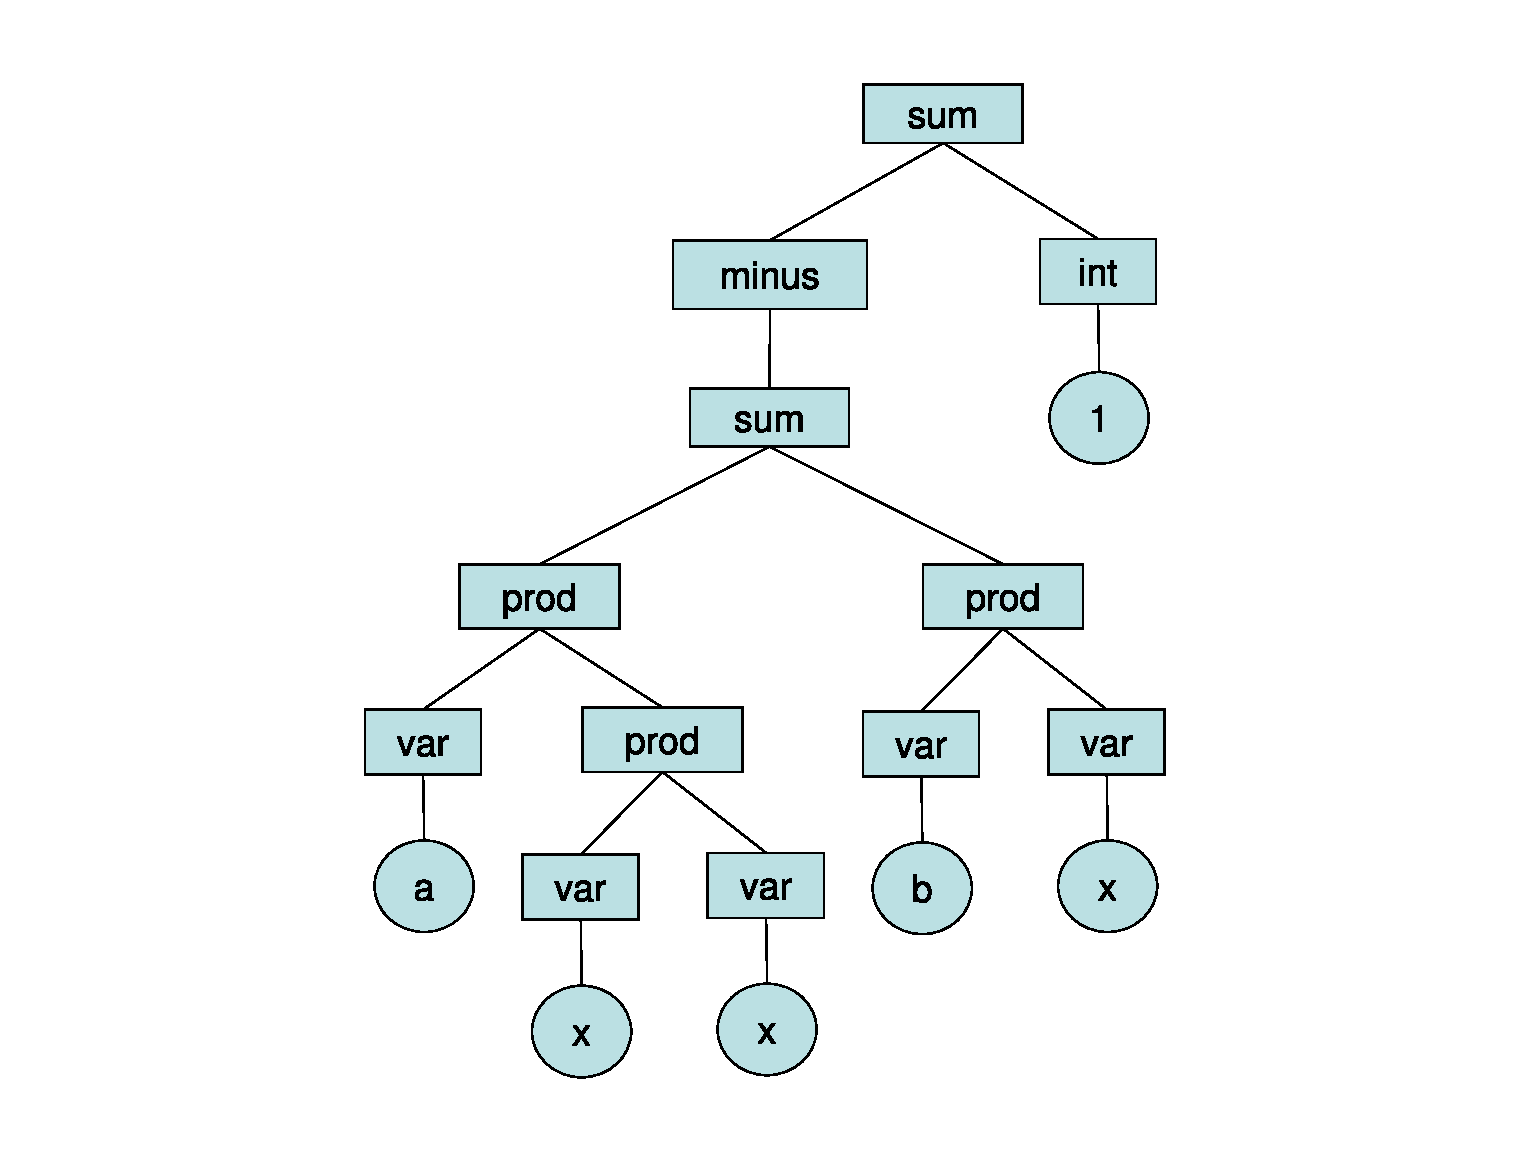
\includegraphics[width=5in]{parsetree}
\caption{Parse tree for $-(a(x\cdot x)+ bx) + 1$.}
\label{fig:parse}
\end{figure}

In a computer, such a tree would be represented by pairs or triples
that begin with a
\emph{tag} equal to the label of the top node of the parse tree.  
The general definition of parse trees for $\aexp$'s would be:

%\newcommand{\paexp}{\text{Aexp-parse-tree}}

\begin{definition}\label{arithparse}
The set $\paexp$ of \emph{parse trees for arithmetic expressions} 
over a set of
\emph{variables} $V$ is defined recursively as follows:
\begin{itemize}
\item \inductioncase{Base cases}:
\begin{enumerate}
\item If $n \in \integers$, then $\ang{\texttt{int}, n} \in \paexp$.
\item If $v \in V$, then $\ang{\texttt{var}, v} \in \paexp$.
\end{enumerate}
\item \inductioncase{Constructor cases}: if $e,e' \in \paexp$, then
\begin{enumerate}
\item $\ang{\texttt{sum}, e, e'} \in \paexp$,
\item $\ang{\texttt{prod}, e, e'} \in \paexp$, and
\item $\ang{\texttt{minus}, e} \in \paexp$.
\end{enumerate}
\end{itemize}
\end{definition}

So the $\paexp$ corresponding to formula~\ref{ax} would be:
\begin{equation}\label{axtag}
\begin{array}{rll}
\left< \right. \texttt{sum}, 
         & \left< \right. \texttt{minus},\ \ \left< \right. \texttt{sum},
               & \ang{\texttt{prod},\ \ \ang{\texttt{var},\ a},
                                     \ang{\texttt{prod},\ \
                                            \ang{\texttt{var},\ x},\
                                            \ang{\texttt{var},\ x}}},\\
                               && \left. \left. \ang{\texttt{prod},\ \
                                       \ang{\texttt{var},\ b},\
                                       \ang{\texttt{var},\ x}}
                                   \right> \right>,\\
         & \left. \left. \ang{\texttt{int},\ 1} \right> \right>
\end{array}
\end{equation}
Now the expression~\ref{ax} is certainly a lot more humanly
intelligible than~\ref{axtag}, but~\ref{axtag} is in the
representation best suited and commonly used in compiling and
processing computer programs.

\end{editingnotes}

\endinput



%% with subtrees as shown in Figure~\ref{rotate2} and values as indicated
%% by integers corresponding to those in Figure~\ref{rotate1}. 

%%  If both are depth $d+1$, then let $U$ be the one
%% with values.  If the depth of $U$ is $d+1$,
%% then it must have branches $C,D$ of depths $d,d-1$ with at least one
%% $d$.  In this case, we re-arrange as shown in (on the right below).
%% Otherwise, the depth of $U$ is $d$ and of $R$ is $d+1$, in which case
%% $R$ must in turn have a branches $V,W$ of depths $d$ or $d-1$ with at
%% least one $d$.  This is illustrated in Figure~\ref{rotate1} with
%% integer labels corresponding to the relative values of the labels of
%% these trees.
%%                                        X6                  
%%                          d+1,2  Z2             y7  d+1    
%%                               1   4        C6.6  D8     
  
%% \begin{figure}
%% \begin{verbatim}
%%                              N2                 
%%                              /\
%%                             /  \
%%                           B1   S4
%%                                /\
%%                               /  \
%%                              /    \
%%                             /      \
%%                           R3        U5
%% \end{verbatim}

%% \caption{Tree before rotation.}

%% \label{rotate1}

%% \end{figure}

%% In Figure~\ref{rotate1},
%% \begin{align*}
%% \dpth{B} & = d\\
%% \dpth{S} & = d+2,\\
%% \dpht{R} & = d+1,\\
%% \dpht{U} & = d\\
%% \dpht{V} & = d,\\
%% \dpht{W} \in  \set{d, d-1}.\\
%% \end{align*}

%% The result of the rotation is defined to be three new trees $X,Y,Z$
%% with subtrees as shown in Figure~\ref{rotate2} and values as indicated
%% by integers corresponding to those in Figure~\ref{rotate1}.  That is,
%% \begin{align*}
%% \nlbl{X}  & = \nlbl{R},\\
%% \nlbl{Y}  & = \nlbl{N}  & = \nlbl{T},\\
%% \nlbl{Z}  &= \nlbl{S},\\
%% \dpth{Y} & = d+1,\\
%% \dpth{Z} & = d+1,
%% \end{align*}

%% \begin{figure}

%% %\graphic{}

%% \begin{verbatim}
%%            X4                         X4                                     N2                 
%%            /\                         /\                                     /\                 
%%           /  \                       /  \                                   /  \                
%%          /    \                     /    \                              d  B1   S6 d+2
%%        Y2      Z6                 Y2      Z6                                   /\               
%%        /\      /\                 /\      /\                                  /  \              
%%       /  \    /  \               /  \    /  \                       d,d+1   R4   U7 d+1
%%      B1  V3  W5  U7             B1  V3  C6.5  D8                            / \                 
%% \end{verbatim}                                                             /   \                
%%                                                                          V3     W5    C6.5   D8 
%% \caption{Tree after rotation is AVL.}

%% \label{rotate2}                                                    
                                                                   
%% \end{figure}                                                       


\iffalse
Of course, the only sensible
move at this point for the first player is to choose to remove all
three stones.  In other words, the first
player chooses $\nimg{\emptystring} \in O_{\ang{3}}$ leaving the
second player to choose a Nim game in
\[
O_{\emptystring} \eqdef \emptyset.
\]
Since there is no Nim game in $O_{\emptystring}$, the second player
loses.

\[
(2, 3)
\]

\[
\set{\text{(2), (3), (1 2), (1 3), (2 2)}}
\]

\[
\set{\set{\emptyset, \text{(1)}},\ \ \set{\set{\text{(2), (1 2)}}},\ \ \set{\emptyset, \text{(1), (2)}},\ \ \set{\text{(1), (2), (1 1)}},\ \ \set{\text{(1), (3), (1 1), (1 2)}}}
\]


Now the last game
\[
\set{\text{(1), (3), (1 1), (1 2)}}
\]
expands again to
\[
\set{\set{\emptyset},\ \ \set{\emptyset, \text{(1),
      (2)}},\ \ \set{\text{(1)}},\ \ \set{\text{(1), (2), (1 1)}}}.
\]


Now the second game, 
\[
\set{\set{\text{(2), (1 2)}}}
\]
for example, expands again to
\[
\set{\set{\emptyset, \text{(1)}},\ \ \set{\text{(1), (2), (1 1)}}}
\]
\fi
 %structural induction, value-games


\chapter{Number Theory}\label{number_theory_chap}

\term{Number theory} is the study of the integers.  \emph{Why} anyone
would want to study the integers is not immediately obvious.  First of
all, what's to know?  There's 0, there's 1, 2, 3, and so on, and, oh
yeah, -1, -2, \dots.  Which one don't you understand?  Second, what
practical value is there in it?

\iffalse Number theory is at the core of mathematics; even Ug the
Caveman surely had some grasp of the integers ---at least the positive
ones.  In fact, the integers are so elementary that one might ask,
``What's to study?''  There's 0, there's 1, 2, 3 and so on, and
there's the negatives.  Which one don't you understand?  Doesn't math
become easy when we don't have to worry about nasty numbers like
$\sqrt{7}$, $1 / \pi$, and $i$?  We can even forget about fractions!
\fi

The mathematician G. H. \idx{Hardy} delighted at its impracticality; he wrote:

 \begin{quotation}
 \noindent [Number theorists] may be justified in rejoicing that there
 is one science, at any rate, and that their own, whose very
 remoteness from ordinary human activities should keep it gentle and
 clean.
 \end{quotation}

Hardy was specially concerned that number theory not be used in
warfare; he was a pacifist.  You may applaud his sentiments, but he
got it wrong: number theory underlies modern cryptography, which is
what makes secure online communication possible.  Secure communication
is of course crucial in war ---which may leave poor Hardy spinning in
his grave.  It's also central to online commerce.  Every time you buy
a book from Amazon, use a certificate to access a web page, or use a
PayPal account, you are relying on number theoretic algorithms.

Number theory also provides an excellent environment for us to
practice and apply the proof techniques that we developed in previous
chapters.  We'll work out properties of \idx{greatest common divisors}
(gcd's) and use them to prove that integers factor uniquely into
primes.  Then we'll introduce modular arithmetic and work out enough
of its properties to explain the \idx{RSA public key crypto-system}.

%~\ref{templates_chap} and~\ref{induction_chap}.

Since we'll be focusing on properties of the integers, we'll adopt the
default convention in this chapter that \textbf{variables range over
  the set, $\integers$, of integers}.

\section{Divisibility}\label{divisibility_sec}

The nature of number theory emerges as soon as we consider the divides relation.
\begin{definition}\label{divides_def}
$a$ \term{divides} $b$ (notation $a \divides b$) iff there an integer $k$ such that
\[
ak = b.
\]
\end{definition}
The divides relation comes up so frequently that multiple synonyms for it are used all the
time.  The following phrases all say the same thing:
\begin{itemize}
\item $a \divides b$,
\item $a$ divides $b$,
\item $a$ is a \term{divisor} of $b$,
\item $a$ is a \term{factor} of $b$,
\item $b$ is \term{divisible} by $a$,
\item $b$ is a \term{multiple} of $a$.
\end{itemize}
Some immediate consequences of Definition~\ref{divides_def} are that
\[
n  \divides 0,\qquad\qquad
n  \divides n, \text{ and}\qquad\qquad
1  \divides n,
\]
for all $n \neq 0$.

Dividing seems simple enough, but let's play with this definition.  The Pythagoreans, an
ancient sect of mathematical mystics, said that a number is \index{perfect
  number}\term*{perfect} if it equals the sum of its positive integral divisors, excluding
itself.  For example, $6 = 1 + 2 + 3$ and $28 = 1 + 2 + 4 + 7 + 14$ are perfect numbers.
On the other hand, 10 is not perfect because $1 + 2 + 5 = 8$, and 12 is not perfect because
$1 + 2 + 3 + 4 + 6 = 16$.  \idx{Euclid} characterized all the \emph{even} perfect numbers
around 300 BC (see Problem~\ref{CP_perfect_numbers}).  But is there an \emph{odd} perfect
number?  More than two thousand years later, we still don't know!  All numbers up to about
$10^{300}$ have been ruled out, but no one has proved that there isn't an odd perfect
number waiting just over the horizon.

So a half-page into number theory, we've strayed past the outer limits of human knowledge!
This is pretty typical; number theory is full of questions that are easy to pose, but
incredibly difficult to answer.  We'll mention a few more such questions in later
sections.\footnote{\emph{Don't Panic} ---we're going to stick to some relatively benign
  parts of number theory.  These super-hard unsolved problems rarely get put on problem
  sets.}

\subsection{Facts about Divisibility}

The following lemma collects some basic facts about divisibility.

\begin{lemma}\label{lem:div}\mbox{}
\begin{enumerate}
%\item If $a \divides b$, then $a \divides bc$ for all $c$.

\item\label{lem:divtrans} If $a \divides b$ and $b \divides c$, then $a \divides c$.

\item\label{lem:divsbtc} If $a \divides b$ and $a \divides c$, then $a \divides sb + tc$
  for all $s$ and $t$.

\item\label{lem:divcancel} For all $c \neq 0$, $a \divides b$ if and only if $ca \divides
  cb$.
\end{enumerate}
\end{lemma}

\begin{proof}
These facts all follow directly from Definition~\ref{divides_def}.  To
illustrate this, we'll prove just part~\ref{lem:divsbtc}:

Given that $a \divides b$, there is some $k_1 \in \integers$ such that $a k_1 = b$.
Likewise, $a k_2 = c$, so
\[
sb+tc= s(k_1a) + t(k_2a) = (sk_1+tk_2)a.
\]
Therefore $sb+tc = k_3a$ where $k_3 \eqdef (sk_1+tk_2)$, which means that
\[
a \divides sb+tc.
\]
\end{proof}

A number of the form $sb+tc$ is called an \term{integer linear
  combination} of $b$ and $c$, or a plain \emph{linear combination},
since in this chapter we're only talking about integers.  So
Lemma~\ref{lem:div}.\ref{lem:divsbtc} can be rephrased as
\begin{quote}
If $a$ divides $b$ and $c$, then $a$ divides every linear combination
of $b$ and~$c$.
\end{quote}
We'll be making good use of linear combinations, so let's get the
general definition on record:
\begin{definition}\label{linear_def}
An integer $n$ is a \term{linear combination} of numbers $b_0,\dots,b_k$ iff
\[
n = s_0b_0+s_1b_1+\cdots+s_kb_k
\]
for some integers $s_0,\dots,s_k$.
\end{definition}

\subsection{When Divisibility Goes Bad}

As you learned in elementary school, if one number does \emph{not}
evenly divide another, you get a ``quotient'' and a ``remainder'' left
over.  More precisely:
\begin{theorem}\label{division_thm}[\idx{Division Theorem}]%
\footnote{This theorem is often called the ``Division Algorithm,'' but
  mwe prefer to call it a theorem since it does not actually describe
  a division procedure for computing the quotient and remainder.}  Let
$n$ and $d$ be integers such that $d > 0$.  Then there exists a unique
pair of integers $q$ and $r$, such that
\begin{equation}\label{nqdr}
n = q \cdot d + r \QAND\ 0 \leq r < d.
\end{equation}
\end{theorem}
The number $q$ is called the \term{quotient} and the number $r$ is
called the \term{remainder} of $n$ divided by $d$.  We use the
notation $\qcnt{n}{d}$ for the quotient and $\rem{n}{d}$ for the
remainder. For example, $\qcnt{2716}{10} = 271$ and $\rem{2716}{10} =
6$, since $2716 = 271 \cdot 10 + 6$.  Similarly, $\rem{-11}{7} = 3$,
since $-11 = (-2) \cdot 7 + 3$.

There is a remainder operator built into many programming languages.
For example, ``32~\%~5'' will be familiar as remainder notation to
programmers in Java, C, and C++; it evaluates to $\rem{32}{5} =2$ in
all three languages.  On the other hand, these languages treat
remainders involving negative numbers idiosyncratically, so if you
program in one those languages, remember to stick to the definition
according to the Division Theorem~\ref{division_thm}.

The remainder on division by $n$ is a number in the (integer)
\term{interval} from 0 to $n-1$.  Such intervals come up so often that
it is useful to have a simple notation for them.
\begin{align*}
(k, n) & \eqdef\quad \set{i \suchthat k < i < n},\\
(k, n] & \eqdef\quad (k,n) \union \set{n},\\
[k, n) & \eqdef\quad \set{k} \union (k,n),\\
[k,n] & \eqdef\quad \set{k} \union (k,n) \union \set{n} = \set{i \suchthat k \leq i \leq n}.
\end{align*}

\subsection{Die Hard}

\emph{Die Hard~3} is just a B-grade action movie, but we think it has
an inner message: everyone should learn at least a little number
theory.  In Section~\ref{diehard_machine}, we formalized a state
machine for the \idx{Die Hard} jug-filling problem using 3 and 5
gallon jugs, and also with 3 and 9 gallon jugs, and came to different
conclusions about bomb explosions.  What's going on in general?  For
example, how about getting 4 gallons from 12- and 18-gallon jugs,
getting 32 gallons with 899- and 1147-gallon jugs, or getting 3
gallons into a jug using just 21- and 26-gallon jugs?

\begin{editingnotes}
Unfortunately, Hollywood never lets go of a gimmick.  Although there
were no water jug tests in \emph{Die Hard~4: Live Free or Die Hard},
rumor has it that the jugs will return in future sequels:
\begin{description}

\item[Die Hard~5: Die Hardest] Bruce goes on vacation and ---shockingly ---happens into a
  terrorist plot.  To save the day, he must make 3~gallons using 21- and 26-gallon jugs.

\item[Die Hard~6: Die of Old Age] Bruce must save his assisted living facility from a
  criminal mastermind by forming 2 gallons with 899- and 1147-gallon jugs.

\item[Die Hard~7: Die Once and For All] Bruce has to make 4 gallons using 3- and 6-gallon
  jugs.

\end{description}
\end{editingnotes}

It would be nice if we could solve all these silly water jug questions at once.  \iffalse
In particular, how can one form $g$ gallons using jugs with capacities $a$ and~$b$?\fi This
is where number theory comes in handy.

\subsubsection{A Water Jug \idx{Invariant}}\label{jug_invar_subsubsec}

Suppose that we have water jugs with capacities $a$ and $b$ with $b
\geq a$.  Let's carry out some sample operations of the state machine
and see what happens, assuming the $b$-jug is big enough:
\begin{align*}
(0,0) & \rightarrow (a,0) & \text{fill first jug} \\
& \rightarrow (0,a) & \text{pour first
    into second} \\
& \rightarrow (a, a) & \text{fill first jug} \\
& \rightarrow (2a-b, b)
  & \text{pour first into second (assuming $2a \geq b$)} \\
& \rightarrow (2a-b, 0) &
  \text{empty second jug} \\
& \rightarrow (0, 2a-b) & \text{pour first into second} \\
&
  \rightarrow (a, 2a-b) & \text{fill first} \\
& \rightarrow (3a-2b, b) & \text{pour first
    into second (assuming $3a \geq 2b$)}
\end{align*}
What leaps out is that at every step, the amount of water in each jug
is of a linear combination of $a$ and $b$.  This is easy to prove by
induction on the number of transitions:
\begin{lemma}[Water Jugs]\label{lem:waterjugs}
In the \emph{\idx{Die Hard}} state machine of
Section~\ref{diehard_machine} with jugs of sizes $a$ and $b$, the
amount of water in each jug is always a linear combination of $a$ and
$b$.
\end{lemma}

\begin{proof}
The induction hypothesis, $P(n)$, is the proposition that after $n$
transitions, the amount of water in each jug is a linear combination
of $a$ and $b$.

\inductioncase{Base case} ($n = 0$): $P(0)$ is true, because both jugs are initially empty,
and $0 \cdot a + 0 \cdot b = 0$.

\inductioncase{Inductive step}: Suppose the machine is in state
$(x,y)$ after $n$ steps, that is, the little jug contains $x$ gallons
and the big one contains $y$ gallons.  There are two cases:

\begin{itemize}

\item If we fill a jug from the fountain or empty a jug into the
  fountain, then that jug is empty or full.  The amount in the other
  jug remains a linear combination of $a$ and $b$.  So $P(n+1)$ holds.

\item Otherwise, we pour water from one jug to another until one is
  empty or the other is full.  By our assumption, the amount $x$ and
  $y$ in each jug is a linear combination of $a$ and $b$ before we
  begin pouring.  After pouring, one jug is either empty (contains 0
  gallons) or full (contains $a$ or $b$ gallons).  Thus, the other jug
  contains either $x + y$ gallons, $x + y - a$, or $x + y - b$
  gallons, all of which are linear combinations of $a$ and $b$ since
  $x$ and $y$ are.  So $P(n+1)$ holds in this case as well.
\end{itemize}
Since $P(n+1)$ holds in any case, this proves the inductive step, completing the proof by
induction.
\end{proof}

So we have established that the jug problem has a preserved invariant,
namely, the amount of water in every jug is a linear combination of
the capacities of the jugs.  Lemma~\ref{lem:waterjugs} has an
important corollary:
\begin{corollary*}
Getting 4 gallons from 12- and 18-gallon jugs, and likewise getting 32
gallons from 899- and 1147-gallon jugs,
\begin{center}
\textbf{Bruce dies!}
\end{center}
\end{corollary*}

\begin{proof}
By the Water Jugs Lemma~\ref{lem:waterjugs}, with 12- and 18-gallon
jugs, the amount in any jug is a linear combination of 12 and 18.
This is always a multiple of 6 by
Lemma~\ref{lem:div}.\ref{lem:divsbtc}, so Bruce can't get 4 gallons.
Likewise, the amount in any jug using 899- and 1147-gallon jugs is a
multiple of 31, so he can't get 32 either.
\end{proof}

But the Water Jugs Lemma doesn't tell the complete story.  For
example, it leaves open the question of getting 3 gallons into a jug
using just 21- and 26-gallon jugs: the only positive factor of both 21
and 26 is 1, and of course 1 divides 3, so the Lemma neither rules out
nor confirms the possibility of getting 3 gallons.

A bigger issue is that we've just managed to recast a pretty
understandable question about water jugs into a technical question
about linear combinations.  This might not seem like a lot of
progress.  Fortunately, linear combinations are closely related to
something more familiar, namely greatest common divisors, and these
will help us solve the general water jug problem.

\begin{problems}
\practiceproblems
\pinput{TP_linear-combs-combined}
\pinput{TP_Inverse_with_Linear_Combinations}

\classproblems
\pinput{CP_perfect_numbers}

\end{problems}

\section{The Greatest Common Divisor}\label{sec:gcd}

A \term{common divisor} of~$a$ and~$b$ is a number that divides them
both.  The \term{greatest common divisor} of $a$ and~$b$ is written
\index{gcd} $\gcd(a, b)$.  For example, $\gcd(18, 24) = 6$.

As long as $a$ and $b$ are not both 0, they will have a gcd. The gcd
turns out to be a very valuable piece of information about the
relationship between $a$ and $b$ and for reasoning about integers in
general.  We'll be making lots of use of gcd's in what follows.

Some immediate consequences of the definition of gcd are that for $n > 0$,
\[
\gcd(n, n) = n, \qquad \gcd(n, 1) = 1, \text{and} \qquad  \gcd(n,0) = n,
\]
where the last equality follows from the fact that everything is a
divisor of 0.

\iffalse
\begin{editingnotes}
\subsection{\idx{Linear Combinations} and the \idx{GCD}}

The theorem below relates the greatest common divisor to linear
combinations.  This theorem is \emph{very} useful; take the time to
understand it and then remember it!

\begin{theorem} \label{th:gcd} The greatest common divisor of $a$ and $b$ is equal to
the smallest positive linear combination of $a$ and $b$.
\end{theorem}

For example, the greatest common divisor of 52 and 44 is 4.  And, sure
enough, 4 is a linear combination of 52 and 44:
\[
6 \cdot 52 + (-7) \cdot 44 = 4
\]
Furthermore, no linear combination of 52 and 44 is equal to a smaller
positive integer.

\begin{proof}[Proof of Theorem~\ref{th:gcd}]
By the Well Ordering Principle, there is a smallest positive linear
combination of $a$ and $b$; call it $m$.  We'll prove that $m =
\gcd(a, b)$ by showing both $\gcd(a, b) \leq m$ and $m \leq \gcd(a,
b)$.

First, we show that $\gcd(a, b) \leq m$.  Now any common divisor of
$a$ and $b$ ---that is, any $c$ such that $c \divides a$ and $c
\divides b$ ---will divide both $sa$ and $tb$, and therefore also
$sa+tb$ for any $s$ and~$t$.  The $\gcd(a, b)$ is by definition a
common divisor of $a$ and $b$, so
\begin{equation}\label{gcdabdivlin} \gcd(a, b)
\divides s a + t b
\end{equation}
for every $s$ and $t$.  In particular, $\gcd(a, b) \divides m$, which
implies that $\gcd(a, b) \leq m$.

Now, we show that $m \leq \gcd(a, b)$.  We do this by showing that $m
\divides a$.  A symmetric argument shows that $m \divides b$, which
means that $m$ is a common divisor of $a$ and $b$.  Thus, $m$ must be
less than or equal to the \emph{greatest} common divisor of $a$ and
$b$.

All that remains is to show that $m \divides a$.  By the Division
Theorem, there exists a quotient $q$ and remainder $r$ such that:
\[
a = q \cdot m + r \hspace{1in} \text{(where $0 \leq r < m$)} \] Recall
that $m = s a + t b$ for some integers $s$ and $t$.  Substituting in
for $m$ gives:
\begin{align*} a & = q \cdot (s a + t b) + r,
\qquad \text{so} \\
r & = (1 - qs) a + (-qt) b.
\end{align*}
We've just expressed $r$ as a linear combination of $a$ and $b$.
However, $m$ is the \emph{smallest positive} linear combination and $0
\leq r < m$.  The only possibility is that the remainder $r$ is not
positive; that is, $r = 0$.  This implies $m \divides a$.  \end{proof}

\begin{corollary}\label{cor:lin-comb-edit}
An integer is linear combination of $a$ and $b$ iff it is a multiple
of $\gcd(a, b)$.
\end{corollary}

\begin{proof} By~\eqref{gcdabdivlin}, every linear combination of $a$ and $b$ is a
multiple of $\gcd(a, b)$.  Conversely, since $\gcd(a, b)$ is a linear
combination of $a$ and $b$, every multiple of $\gcd(a, b)$ is as
well.  \end{proof}

Now we can restate the water jugs lemma in terms of the greatest
common divisor:

\begin{corollary} \label{cor:waterjugs_note} Suppose that we have water jugs with
capacities $a$ and $b$.  Then the amount of water in each jug is
always a multiple of $\gcd(a, b)$.
\end{corollary}

For example, there is no way to form 4 gallons using 3- and 6-gallon
jugs, because 4 is not a multiple of $\gcd(3, 6) = 3$.

\end{editingnotes}
\fi

\subsection{Euclid's Algorithm}
The first thing to figure out is how to find gcd's.  A good way called \term{Euclid's
  Algorithm} has been known for several thousand years.  It is based on the following
elementary observation.

\begin{lemma}\label{lem:gcdrem}
For $b \neq 0$,
\[
\gcd(a, b) = \gcd(b, \rem{a}{b}).
\]

\begin{proof}
By the Division Theorem~\ref{division_thm},
\begin{equation}\label{aqbrprf}
a = qb + r
\end{equation}
where $r = \rem{a}{b}$.  So $a$ is a linear combination of $b$ and
$r$, which implies that any divisor of $b$ and $r$ is a divisor of $a$
by Lemma~\ref{lem:div}.\ref{lem:divsbtc}.  Likewise, $r$ is a linear
combination, $a-qb$, of $a$ and $b$, so any divisor of $a$ and $b$ is
a divisor of $r$.  This means that $a$ and $b$ have the same common
divisors as $b$ and $r$, and so they have the same \emph{greatest}
common divisor.
\end{proof}
\end{lemma}

Lemma~\ref{lem:gcdrem} is useful for quickly computing the greatest
common divisor of two numbers.  For example, we could compute the
greatest common divisor of 1147 and~899 by repeatedly applying it:
\begin{align*}
\gcd(1147, 899) &= \gcd\paren{899, \underbrace{\rem{1147}{899}}_{{} = 248}} \\
&= \gcd\paren{248, \rem{899}{248} = 155} \\
&= \gcd\paren{155, \rem{248}{155} = 93} \\
&= \gcd\paren{ 93, \rem{155}{93} = 62}\\
&= \gcd\paren{ 62, \rem{93}{62} = 31} \\
&= \gcd\paren{ 31, \rem{62}{31} = 0} \\
&= 31
\end{align*}
This calculation that $\gcd(1147, 899) = 31$ was how we figured out
that with water jugs of sizes 1147 and 899, Bruce dies trying to get
32 gallons.

On the other hand, applying Euclid's algorithm to 26 and 21 gives
\[
\gcd(26, 21) = \gcd(21, 5) = \gcd(5, 1) = 1,
\]
so we can't use the reasoning above to rule out Bruce getting 3
gallons into the big jug.  As a matter of fact, because the gcd here
is 1, Bruce \emph{will} be able to get any number of gallons into the big jug
up to its capacity.  To explain this, we will need a little more
number theory.

\subsubsection{Euclid's Algorithm as a State Machine}
By the way, Euclid's algorithm can easily be formalized as a state
machine.  The set of states is $\naturals^2$ and there is one
transition rule:
\begin{equation}\label{euclid_transition}
(x,y) \movesto (y, \rem{x}{y}),
\end{equation}
for $y>0$.  By Lemma~\ref{lem:gcdrem}, the gcd stays the same from one
state to the next.  That means the predicate
\[
\gcd(x,y) = \gcd(a,b)
\]
is a preserved invariant on the states $(x,y)$.  This preserved
invariant is, of course, true in the start state $(a,b)$.  So by the
Invariant Principle, if $y$ ever becomes $0$, the invariant will be
true and so
\[
x = \gcd(x,0) = \gcd(a,b).
\]
Namely, the value of $x$ will be the desired gcd.

What's more, $x$, and therefore also $y$, gets to be 0 pretty fast.
To see why, note that starting from $(x,y)$, two transitions leads to
a state whose the first coordinate is $\rem{x}{y}$, which is at most
half the size of $x$.\footnote{In other words,
\begin{equation}\label{rxylx2}
\rem{x}{y} \le x/2 \qquad \text{for $0 < y \le x$}.
\end{equation}
This is immediate if $y \le x/2$, since the remainder of $x$ divided
by $y$ is less than $y$ by definition.  On the other hand, if $y >
x/2$, then $\rem{x}{y} = x - y < x/2$.}  Since $x$ starts off equal to
$a$ and gets halved or smaller every two steps, it will reach its
minimum value ---which is $\gcd(a,b)$ ---after at most $2 \log a$
transitions.  After that, the algorithm takes at most one more
transition to terminate.  In other words, Euclid's algorithm
terminates after at most $1+2 \log a$ transitions.\footnote{A tighter
  analysis shows that at most $\log_\varphi(a)$ transitions are
  possible where $\varphi$ is the \term{golden ratio} $(1 +
  \sqrt{5})/2$, see Problem~\ref{PS_gcd_termination}.}

\subsection{The Pulverizer}\label{sec:pulverizer}
We will get a lot of mileage out of the following key fact:
\begin{theorem}\label{gcd_is_lin_thm}
The greatest common divisor of $a$ and $b$ is a linear combination of
$a$ and~$b$.  That is,
\[
\gcd(a, b) = s a + t b,
\]
for some integers $s$ and $t$.
\end{theorem}

We already know from Lemma~\ref{lem:div}.\ref{lem:divsbtc} that every
linear combination of $a$ and $b$ is divisible by any common factor of
$a$ and $b$, so it is certainly divisible by the greatest of these
common divisors.  Since any constant multiple of a linear combination
is also a linear combination, Theorem~\ref{gcd_is_lin_thm} implies
that any multiple of the gcd is a linear combination, giving:
\begin{corollary}\label{cor:lin-comb}
An integer is a linear combination of $a$ and $b$ iff it is a multiple
of $\gcd(a, b)$.
\end{corollary}

We'll prove Theorem~\ref{gcd_is_lin_thm} directly by explaining how to
find $s$ and $t$.  This job is tackled by a mathematical tool that
dates back to sixth-century India, where it was called \emph{kuttak},
which means ``The Pulverizer.''  Today, the Pulverizer is more
commonly known as ``the extended Euclidean GCD algorithm,'' because it
is so close to Euclid's Algorithm.

For example, following Euclid's Algorithm, we can compute the GCD of
259 and~70 as follows:
\begin{align*}
\gcd(259, 70) & = \gcd(70, 49) & \quad & \text{since $\rem{259}{70} = 49$}\\
 & = \gcd(49, 21) && \text{since $\rem{70}{49} = 21$} \\
 & = \gcd(21, 7) && \text{since $\rem{49}{21} = 7$} \\
 & = \gcd(7, 0)
                && \text{since $\rem{21}{7} = 0$} \\
 & = 7.
\end{align*}
The Pulverizer goes through the same steps, but requires some extra
bookkeeping along the way: as we compute $\gcd(a, b)$, we keep track
of how to write each of the remainders (49, 21, and 7, in the example)
as a linear combination of $a$ and $b$.  This is worthwhile, because
our objective is to write the last nonzero remainder, which is the
GCD, as such a linear combination.  For our example, here is this
extra bookkeeping:
\[
\begin{array}{ccccrcl}
x & \quad & y & \quad & (\rem{x}{y}) & = & x - q \cdot y \\
\hline
259 && 70 && 49 & = & 259 - 3 \cdot 70 \\
 70 && 49 && 21 & = & 70 - 1 \cdot 49 \\
           &&&& & = & 70 - 1 \cdot (259 - 3 \cdot 70) \\
           &&&& & = & -1 \cdot 259 + 4 \cdot 70 \\
 49 && 21 && 7  & = & 49 - 2 \cdot 21\\
           &&&& & = & (259 - 3 \cdot 70) - 2 \cdot (-1 \cdot 259 + 4 \cdot 70) \\
           &&&& & = & \fbox{$3 \cdot 259 - 11 \cdot 70$} \\
 21 && 7 && 0
\end{array}
\]
We began by initializing two variables, $x = a$ and $y = b$.  In the
first two columns above, we carried out Euclid's algorithm.  At each
step, we computed $\rem{x}{y}$ which equals $x - \qcnt{x}{y} \cdot y$.
Then, in this linear combination of $x$ and $y$, we replaced $x$ and
$y$ by equivalent linear combinations of $a$ and $b$, which we already
had computed.  After simplifying, we were left with a linear
combination of $a$ and $b$ equal to $\rem{x}{y}$, as desired.  The
final solution is boxed.

This should make it pretty clear how and why the Pulverizer works.
Anyone if you have doubts, work through
Problem~\ref{PS_pulverizer_machine}, where the Pulverizer is
formalized as a state machine and then verified using an invariant
that is an extension of the one used for Euclid's algorithm.

Since the Pulverizer requires only a little more computation than
Euclid's algorithm, you can ``pulverize'' very large numbers very
quickly by using this algorithm.  As we will soon see, its speed makes
the Pulverizer a very useful tool in the field of cryptography.

Now we can restate the Water Jugs Lemma~\ref{lem:waterjugs} in terms
of the greatest common divisor:
\begin{corollary}\label{cor:waterjugs}
Suppose that we have water jugs with capacities $a$ and $b$.  Then the
amount of water in each jug is always a multiple of $\gcd(a, b)$.
\end{corollary}

For example, there is no way to form 4 gallons using 3- and 6-gallon
jugs, because 4 is not a multiple of $\gcd(3, 6) = 3$.

\subsection{One Solution for All Water Jug Problems}\label{all_jugs_son_sec}

Corollary~\ref{cor:lin-comb} says that 3 can be written as a linear
combination of 21 and 26, since 3 is a multiple of $\gcd(21, 26) = 1$.
So the Pulverizer will give us integers $s$ and $t$ such that
\begin{equation}\label{3s21t26}
3 = s \cdot 21 + t \cdot 26
\end{equation}

Now the coefficient $s$ could be either positive or negative.
However, we can readily transform this linear combination into an
equivalent linear combination
\begin{equation}\label{3sprime21}
3 = s' \cdot 21 + t' \cdot 26
\end{equation}
where the coefficient $s'$ is positive.  The trick is to notice that
if in equation~\eqref{3s21t26} we increase $s$ by 26 and decrease $t$
by 21, then the value of the expression $s \cdot 21 + t \cdot 26$ is
unchanged overall.  Thus, by repeatedly increasing the value of $s$
(by 26 at a time) and decreasing the value of $t$ (by 21 at a time),
we get a linear combination $s' \cdot 21 + t' \cdot 26 = 3$ where the
coefficient $s'$ is positive.  (Of course $t'$ must then be negative;
otherwise, this expression would be much greater than 3.)

Now we can form 3 gallons using jugs with capacities 21 and~26: We
simply repeat the following steps $s'$ times:
\begin{enumerate}
\item Fill the 21-gallon jug.
\item Pour all the water in the 21-gallon jug into the 26-gallon jug.
  If at any time the 26-gallon jug becomes full, empty it out, and
  continue pouring the 21-gallon jug into the 26-gallon jug.
\end{enumerate}
At the end of this process, we must have have emptied the 26-gallon
jug exactly $-t'$ times.  Here's why: we've taken $s' \cdot 21$
gallons of water from the fountain, and we've poured out some multiple
of 26 gallons.  If we emptied fewer than $-t'$ times, then
by~\eqref{3sprime21}, the big jug would be left with at least $3+26$
gallons, which is more than it can hold; if we emptied it more times,
the big jug would be left containing at most $3-26$ gallons, which is
nonsense.  But once we have emptied the 26-gallon jug exactly $-t'$
times, equation~\eqref{3sprime21} implies that there are exactly 3
gallons left.

Remarkably, we don't even need to know the coefficients $s'$ and $t'$
in order to use this strategy!  Instead of repeating the outer loop
$s'$ times, we could just repeat \emph{until we obtain 3 gallons},
since that must happen eventually.  Of course, we have to keep track
of the amounts in the two jugs so we know when we're done.  Here's the
solution using this approach starting with empty jugs, that is, at
$(0,0)$:
\[
\begin{array}{cccccccc}
\xrightarrow{\text{fill 21}} & (21,0)& \xrightarrow{\text{pour 21 into
    26}} & & & &&(0,21)\\
\xrightarrow{\text{fill 21}} & (21,21)&
\xrightarrow{\text{pour 21 to 26}} & (16,26)& \xrightarrow{\text{empty
    26}} & (16,0)& \xrightarrow{\text{pour 21 to 26}} &
(0,16)\\
\xrightarrow{\text{fill 21}} & (21,16)&
\xrightarrow{\text{pour 21 to 26}} & (11,26)& \xrightarrow{\text{empty
    26}} & (11,0)& \xrightarrow{\text{pour 21 to 26}} &
(0,11)\\
\xrightarrow{\text{fill 21}} & (21,11)&
\xrightarrow{\text{pour 21 to 26}} & (6,26)& \xrightarrow{\text{empty
    26}} & (6,0)& \xrightarrow{\text{pour 21 to 26}} &
(0,6)\\
\xrightarrow{\text{fill 21}} & (21,6)& \xrightarrow{\text{pour
    21 to 26}} & (1,26)& \xrightarrow{\text{empty 26}} & (1,0)&
\xrightarrow{\text{pour 21 to 26}} & (0,1)\\
\xrightarrow{\text{fill
    21}} & (21,1)& \xrightarrow{\text{pour 21 to 26}} &&&&&
(0,22)\\
\xrightarrow{\text{fill 21}} & (21,22)&
\xrightarrow{\text{pour 21 to 26}} & (17,26)& \xrightarrow{\text{empty
    26}} & (17,0)& \xrightarrow{\text{pour 21 to 26}} &
(0,17)\\
\xrightarrow{\text{fill 21}} & (21,17)&
\xrightarrow{\text{pour 21 to 26}} & (12,26)& \xrightarrow{\text{empty
    26}} & (12,0)& \xrightarrow{\text{pour 21 to 26}} &
(0,12)\\
\xrightarrow{\text{fill 21}} & (21,12)&
\xrightarrow{\text{pour 21 to 26}} & (7,26)& \xrightarrow{\text{empty
    26}} & (7,0)& \xrightarrow{\text{pour 21 to 26}} &
(0,7)\\
\xrightarrow{\text{fill 21}} & (21,7)& \xrightarrow{\text{pour
    21 to 26}} & (2,26)& \xrightarrow{\text{empty 26}} & (2,0)&
\xrightarrow{\text{pour 21 to 26}} & (0,2)\\
\xrightarrow{\text{fill
    21}} & (21,2)& \xrightarrow{\text{pour 21 to 26}} &
&&&&(0,23)\\
\xrightarrow{\text{fill 21}} & (21,23)&
\xrightarrow{\text{pour 21 to 26}} & (18,26)& \xrightarrow{\text{empty
    26}} & (18,0)& \xrightarrow{\text{pour 21 to 26}} &
(0,18)\\
\xrightarrow{\text{fill 21}} & (21,18)&
\xrightarrow{\text{pour 21 to 26}} & (13,26)& \xrightarrow{\text{empty
    26}} & (13,0)& \xrightarrow{\text{pour 21 to 26}} &
(0,13)\\
\xrightarrow{\text{fill 21}} & (21,13)&
\xrightarrow{\text{pour 21 to 26}} & (8,26)& \xrightarrow{\text{empty
    26}} & (8,0)& \xrightarrow{\text{pour 21 to 26}} &
(0,8)\\
\xrightarrow{\text{fill 21}} & (21,8)& \xrightarrow{\text{pour
    21 to 26}} & (3,26)& \xrightarrow{\text{empty 26}} & (3,0)&
\xrightarrow{\text{pour 21 to 26}} & (0,3)
\end{array}
\]

The same approach works regardless of the jug capacities and even
regardless the amount we're trying to produce!  Simply repeat these
two steps until the desired amount of water is obtained:
\begin{enumerate}
\item Fill the smaller jug.

\item Pour all the water in the smaller jug into the larger jug.  If
  at any time the larger jug becomes full, empty it out, and continue
  pouring the smaller jug into the larger jug.
\end{enumerate}
By the same reasoning as before, this method eventually generates
every multiple ---up to the size of the larger jug ---of the greatest
common divisor of the jug capacities, namely, all the quantities we
can possibly produce.  No ingenuity is needed at all!

So now we have the complete water jug story:
\begin{theorem}\label{th:waterjugs}
Suppose that we have water jugs with capacities $a$ and $b$.  For any
$c \in [0,a]$, it is possible to get $c$ gallons in the size $a$ jug
iff $c$ is a multiple of $\gcd(a, b)$.
\end{theorem}

\begin{editingnotes}
\subsection{Properties of the \idx{Greatest Common Divisor}}

It can help to have some basic $\gcd$ facts on hand:

\begin{lemma}\label{lem:gcd-hold} 
\begin{enumerate}
%\item Every common divisor of $a$ and $b$ divides $\gcd(a, b)$.
\item\label{gcd2} $\gcd(k a, k b) = k \cdot \gcd(a, b)$ for all $k > 0$.
\item\label{gcd3} If $\gcd(a, b) = 1$ and $\gcd(a, c) = 1$, then $\gcd(a, bc) = 1$.
\item\label{gcd4} If $a \divides b c$ and $\gcd(a, b) = 1$, then $a \divides c$.
%\item\label{gcd5} $\gcd(a, b) = \gcd(b, \rem{a}{b})$. already in lem:gcdrem

\end{enumerate}
\end{lemma}

There is a simple trick for proving these statements:\footnote{These
  properties are all pretty obvious if we assume unique fsctorization
  of integers into primes (Theorem~\ref{thm:unique_factor}), but that
  would be kind of cheating, since haven't proved unique factorization
  yet, and properties like these are needed in the proof of that
  theorem.} translate the $\gcd$ world to the linear combination world
using Theorem~\ref{gcd_is_lin_thm}, argue about linear combinations,
and then translate back using Theorem~\ref{gcd_is_lin_thm} again.

\begin{proof} We prove only parts~\ref{gcd3}.\ and~\ref{gcd4}.

\textbf{Proof of~\ref{gcd3}}.  The assumptions together with
Theorem~\ref{gcd_is_lin_thm} imply that there exist integers $s$, $t$, $u$,
and $v$ such that:
\begin{align*}
s a + t b & = 1 \\
u a + v c & = 1
\end{align*}
Multiplying these two equations gives:
\[
(s a + t b)(u a + v c) = 1
\]
The left side can be rewritten as
\[
a \cdot (a s u + b t u + c s v) + (bc) (t v).
\]
This is a linear combination of $a$ and $b c$ that is equal to 1, so
$\gcd(a, bc) = 1$ by Theorem~\ref{gcd_is_lin_thm}.

\textbf{Proof of~\ref{gcd4}}.  Theorem~\ref{gcd_is_lin_thm} says that
$\gcd(ac, bc)$ is equal to a linear combination of $ac$ and $bc$.  Now
$a \divides ac$ trivially and $a \divides bc$ by assumption.
Therefore, $a$ divides \emph{every} linear combination of $ac$ and
$bc$.  In particular, $a$ divides $\gcd(ac, bc) = c \cdot \gcd(a, b) =
c\cdot 1 = c$.  The first equality uses part~\ref{gcd2}.\ of this
lemma, and the second uses the assumption that $\gcd(a, b) = 1$.
\end{proof}
\end{editingnotes}

\begin{problems}

\practiceproblems
\pinput{TP_GCDs_I}
\pinput{TP_GCDs_II}

\classproblems
\pinput{CP_use_the_pulverizer}
\pinput{CP_proving_basic_gcd_properties}

\homeworkproblems
\pinput{PS_pulverizer_machine}
\pinput{PS_gcd_termination}
\pinput{PS_filling_buckets_with_water}
\pinput{PS_binary_gcd}

\end{problems}

\section{Prime Mysteries}

Some of the greatest mysteries and insights in number theory concern
properties of prime numbers:
\begin{definition}
A \term{prime} is a number greater than~1 that is divisible only by
itself and~1.  A number other than 0, 1, and $-1$ that is not a prime
is called \term{composite}.\footnote{So 0, 1, and $-1$ are the only
  integers that are neither prime nor composite.}
\end{definition}

Here are three famous mysteries:

%\floatingtextbox{ \textboxtitle{Famous Conjectures about Primes}

\begin{description}

\item[\term{Twin Prime Conjecture}] There are infinitely many primes
  $p$ such that $p + 2$ is also a prime.

  In 1966 Chen showed that there are infinitely many primes $p$ such
  that $p + 2$ is the product of at most two primes.  So the
  conjecture is known to be \emph{almost} true!

\item[\term{Conjectured Inefficiency of Factoring}] Given the product
  of two large primes $n = pq$, there is no efficient procedure to
  recover the primes $p$ and $q$.  That is, no \emph{\idx{polynomial
      time}} procedure (see Section~\ref{SAT_sec}) guaranteed to find
  $p$ and $q$ in a number of steps bounded by a polynomial $\log n$,
  which is the number of bits in the binary representation of $n$.

  The best algorithm known is the ``number field sieve,'' which runs
  in time proportional to:
  \[
  e^{1.9(\ln n)^{1/3} (\ln\ln n)^{2/3}}.
  \]
  This number grows more rapidly than any polynomial in $\log n$ and
  is infeasible when $n$ has 300 digits or more.

  Efficient factoring is a mystery of particular importance in
  computer science, as we'll explain later in this chapter.

\item[\term{Goldbach Conjecture}] We've already mentioned Goldbach's
  Conjecture~\ref{Goldbach} several times: every even integer greater
  than two is equal to the sum of two primes.  For example, $4 = 2 +
  2$, $6 = 3 + 3$, $8 = 3 + 5$, etc.

  In 1939 Schnirelman proved that every even number can be written as
  the sum of not more than 300,000 primes, which was a start.  Today,
  we know that every even number is the sum of at most 6 primes.
\end{description}

Primes show up erratically in the sequence of integers.  In fact,
their distribution seems almost random:
\[
2, 3, 5, 7, 11, 13, 17, 19, 23, 29, 31, 37, 41, 43, \dots.
\]
One of the great insights about primes is that their density among the
integers has a precise limit.  Namely, let $\pi(n)$ denote the number
of primes up to $n$:

\begin{definition}\label{def:prime<x}
\[
  \pi(n) \eqdef \card{\set{p \in [2, n] \suchthat p \text{ is
        prime}}}.
\]
\end{definition}

For example, $\pi(1) = 0, \pi(2) = 1$, and $\pi(10) = 4$ because 2, 3,
5, and 7 are the primes less than or equal to 10.  Step by step,
$\pi$ grows erratically according to the erratic spacing between
successive primes, but its overall growth rate is known to smooth out
to be the same as the growth of the function $n/\ln n$:

\begin{theorem}[\term{Prime Number Theorem}]
\[
\lim_{n\to\infty} \frac{\pi(n)}{n/\ln n} = 1.
\]
\end{theorem}

Thus, primes gradually taper off.  As a rule of thumb, about 1 integer
out of every $\ln n$ in the vicinity of $n$ is a prime.

%\begin{editingnotes} The accent on Vallee screwed up the hyphens in
%the entire pdf file!!!  \end{editingnotes}

The Prime Number Theorem was conjectured by Legendre in 1798 and
proved a century later by de la Vallee Poussin and Hadamard in 1896.
However, after his death, a notebook of Gauss was found to contain the
same conjecture, which he apparently made in 1791 at age 15.  (You
sort of have to feel sorry for all the otherwise ``great''
mathematicians who had the misfortune of being contemporaries of
Gauss.)

A proof of the Prime Number Theorem is beyond our scope, but there is
a manageable proof (see Problem~\ref{PS_Chebyshev_prime_bound}) of a
related result that is sufficient for our applications:
\begin{theorem}[Chebyshev's Theorem on Prime Density]
For $n >1$,
\[
\pi(n) > \frac{n}{3 \ln n}.
\]
\end{theorem}

\floatingtextbox{  \textboxheader{A Prime for Google}

In late 2004 a billboard appeared in various locations around the
country:

{\Large
\[
\left\{
\begin{array}{c}
\text{first 10-digit prime found}\\
\text{in consecutive digits of
  $e$}
\end{array}
\right\} \textbf{. com}
\]
}

Substituting the correct number for the expression in curly-braces
produced the URL for a Google employment page.  The idea was that
Google was interested in hiring the sort of people that could and
would solve such a problem.

How hard is this problem?  Would you have to look through thousands or
millions or billions of digits of $e$ to find a 10-digit prime?  The
rule of thumb derived from the Prime Number Theorem says that among
10-digit numbers, about 1 in
\[
\ln 10^{10} \approx 23
\]
is prime.  This suggests that the problem isn't really so hard!  Sure
enough, the first 10-digit prime in consecutive digits of $e$ appears
quite early:
\begin{align*}
e = & 2.718281828459045235360287471352662497757247093699959574966 \\
& 96762772407663035354759457138217852516642\textcolor{blue}{\mathbf{7427466391}}9320030\\
& 599218174135966290435729003342952605956307381323286279434\dots
\end{align*}

%\begin{editingnotes} Checked against
%http://www.gutenberg.org/1/2/127/ --dmj, \end{editingnotes}
}

\begin{problems}
\homeworkproblems
\pinput{PS_Chebyshev_prime_bound}
\end{problems}

\section{The Fundamental Theorem of Arithmetic}\label{fundamental_theorem_sec}

There is an important fact about primes that you probably already
know: every positive integer number has a \emph{unique} prime
factorization.  So every positive integer can be built up from primes
in \emph{exactly one way}.  These quirky prime numbers are the
building blocks for the integers.

Since the value of a product of numbers is the same if the numbers
appear in a different order, there usually isn't a unique way to
express a number as a product of primes.  For example, there are three
ways to write 12 as a product of primes:
\[
12 = 2 \cdot 2 \cdot 3 = 2 \cdot 3 \cdot 2 = 3 \cdot 2 \cdot 2.
\]
What's unique about the prime factorization of 12 is that any product
of primes equal to 12 will have exactly one 3 and two 2's.  This means
that if we \emph{sort} the primes by size, then the product really
will be unique.

Let's state this more carefully.  A sequence of numbers is
\emph{\idx{weakly decreasing}} when each number in the sequence is at
least as big as the numbers after it.  Note that a sequence of just
one number as well as a sequence of no numbers ---the empty sequence
---is weakly decreasing by this definition.

\begin{theorem}\label{thm:unique_factor}[\idx{Fundamental Theorem of Arithmetic}]
Every positive integer is a product of a \emph{unique} weakly
decreasing sequence of primes.
\end{theorem}

For example, 75237393 is the product of the weakly decreasing sequence
of primes
\[
23, 17, 17, 11, 7, 7, 7, 3,
\]
and no other weakly decreasing sequence of primes will give
75237393.\footnote{The ``product'' of just one number is defined to be
  that number, and the product of no numbers is by convention defined
  to be 1.  So each prime, $p$, is uniquely the product of the primes
  in the length-one sequence consisting solely of $p$, and 1, which
  remember is not a prime, is even so uniquely the product of the
  empty sequence.}

Notice that the theorem would be false if 1 were considered a prime;
for example, $15$ could be written as $5 \cdot 3$, or $5 \cdot 3 \cdot
1$, or $5 \cdot 3 \cdot 1 \cdot 1$, \dots.

There is a certain wonder in unique factorization, especially in view
of the prime number mysteries we've already mentioned.  It's a mistake
to take it for granted, even if you've known it since you were in a
crib.  In fact, unique factorization actually fails for many
integer-like sets of numbers, for example, the complex numbers of the
form $n + m\sqrt{-5}$ for $m,n \in \integers$ (see
Problem~\ref{PS_non_unique_factoring}).

The Fundamental Theorem is also called the \term{Unique Factorization
  Theorem}, which is a more descriptive, less pretentious, name ---but
hey, we really want to get your attention to the importance and
non-obviousness of unique factorization.

\subsection{Proving Unique Factorization}

The Fundamental Theorem is not hard to prove, but we'll need a couple
of preliminary facts.

\begin{lemma}
\label{lem:prime-divides}
If $p$ is a prime and $p \divides ab$, then $p \divides a$ or $p
\divides b$.
\end{lemma}

Now Lemma~\ref{lem:prime-divides} follows immediately from Unique
Factorization: the primes in the product $ab$ are exactly the primes
from $a$ and from $b$.  But proving the lemma this way would be
cheating: we're going to need this lemma to prove Unique
Factorization, and it would be circular to assume it.  But there is
another easy way to prove Lemma~\ref{lem:prime-divides} using what we
already know about gcd's and linear combinations.

\begin{proof}
One case is if $\gcd(a, p) = p$.  Then the claim holds, because $a$ is
a multiple of $p$.

Otherwise, $\gcd(a, p) \neq p$.  In this case $\gcd(a, p)$ must be 1,
since 1 and $p$ are the only positive divisors of $p$.  Now $\gcd(a,
p)$ is a linear combination of $a$ and $p$, so we have $1=sa+tp$ for
some $s,t$.  Then $b =s(ab)+ (tb)p$, that is, $b$ is a linear
combination of $ab$ and $p$.  Since $p$ divides both $ab$ and $p$, it
also divides their linear combination $b$.
\end{proof}

A routine induction argument extends this statement to:\iffalse the
fact we assumed last time:\fi

\begin{lemma}
\label{lem:prime-divides-ind}
Let $p$ be a prime.  If $p \divides a_1 a_2 \cdots a_n$, then $p$
divides some $a_i$.
\end{lemma}

Now we're ready to prove the Fundamental Theorem of Arithmetic.
\begin{proof}
Theorem~\ref{factor_into_primes} showed, using the Well Ordering
Principle, that every positive integer can be expressed as a product
of primes.  So we just have to prove this expression is unique.  We
will use Well Ordering to prove this too.

The proof is by contradiction: assume, contrary to the claim, that
there exist positive integers that can be written as products of
primes in more than one way.  By the Well Ordering Principle, there is
a smallest integer with this property.  Call this integer $n$, and let
\begin{align*}
n & = p_1 \cdot p_2 \cdots p_j, \\
& = q_1 \cdot q_2 \cdots q_k,
\end{align*}
where both products are in weakly decreasing order and $p_1 \le q_1$.

If $q_1 = p_1$, then $n/q_1$ would also be the product of different
weakly decreasing sequences of primes, namely,
\begin{align*}
 p_2 \cdots p_j, \\
q_2 \cdots q_k.
\end{align*}
Since $n/q_1 < n$, this can't be true, so we conclude that $p_1 <
q_1$.

Since the $p_i$'s are weakly decreasing, all the $p_i$'s are less than
$q_1$.  But $q_1 \divides n= p_1 \cdot p_2 \cdots p_j$, so
Lemma~\ref{lem:prime-divides-ind} implies that $q_1$ divides one of
the $p_i$'s, which contradicts the fact that $q_1$ is bigger than all
them.
\end{proof}

\begin{problems}
\classproblems \pinput{CP_gcd_lcm}

\homeworkproblems \pinput{PS_non_unique_factoring}

\end{problems}

\section{Alan \idx{Turing}}\label{Turing_sec}

\begin{figure}\redrawntrue
\graphic[width=2in]{turing}
\caption{Alan Turing}
\label{fig:Turing}
\end{figure}

The man pictured in Figure~\ref{fig:Turing} is Alan Turing, the most
important figure in the history of computer science.  For decades, his
fascinating life story was shrouded by government secrecy, societal
taboo, and even his own deceptions.

At age 24, Turing wrote a paper entitled \emph{On Computable Numbers,
  with an Application to the Entscheidungsproblem}.  The crux of the
paper was an elegant way to model a computer in mathematical terms.
This was a breakthrough, because it allowed the tools of mathematics
to be brought to bear on questions of computation.  For example, with
his model in hand, Turing immediately proved that there exist problems
that no computer can solve ---no matter how ingenious the programmer.
Turing's paper is all the more remarkable because he wrote it in 1936,
a full decade before any electronic computer actually existed.

The word ``Entscheidungsproblem'' in the title refers to one of the 28
mathematical problems posed by David Hilbert in 1900 as challenges to
mathematicians of the 20th century.  Turing knocked that one off in
the same paper.  And perhaps you've heard of the ``\idx{Church-Turing
  thesis}''?  Same paper.  So Turing was obviously a brilliant guy who
generated lots of amazing ideas.  But this lecture is about one of
Turing's less-amazing ideas.  It involved codes.  It involved number
theory.  And it was sort of stupid.

%%%%%\subsection{Turing's Code}

Let's look back to the fall of 1937.  Nazi Germany was rearming under
Adolf Hitler, world-shattering war looked imminent, and ---like us
---Alan Turing was pondering the usefulness of number theory.  He
foresaw that preserving military secrets would be vital in the coming
conflict and proposed a way \emph{to encrypt communications using
  number theory}.  This is an idea that has ricocheted up to our own
time.  Today, number theory is the basis for numerous public-key
cryptosystems, digital signature schemes, cryptographic hash
functions, and electronic payment systems.  Furthermore, military
funding agencies are among the biggest investors in cryptographic
research.  Sorry \idx{Hardy}!

Soon after devising his code, \idx{Turing} disappeared from public
view, and half a century would pass before the world learned the full
story of where he'd gone and what he did there.  We'll come back to
Turing's life in a little while; for now, let's investigate the code
Turing left behind.  The details are uncertain, since he never
formally published the idea, so we'll consider a couple of
possibilities.

\subsection{Turing's Code (Version 1.0)}

The first challenge is to translate a text message into an integer so
we can perform mathematical operations on it.  This step is not
intended to make a message harder to read, so the details are not too
important.  Here is one approach: replace each letter of the message
with two digits ($A = 01$, $B = 02$, $C = 03$, etc.) and string all
the digits together to form one huge number.  For example, the message
``victory'' could be translated this way:
\begin{center}
\begin{tabular}{ccccccccc}
   &v & i & c & t & o & r & y \\
$\rightarrow$ & 22 & 09 & 03 & 20 &
  15 & 18 & 25
\end{tabular}
\end{center}
\idx{Turing's code} requires the message to be a prime number, so we
may need to pad the result with some more digits to make a prime.  The
Prime Number Theorem indicates that padding with relatively few digits
will work.  In this case, appending the digits 13 gives the number
2209032015182513, which is prime.

Here is how the encryption process works.  In the description below,
$m$ is the unencoded message (which we want to keep secret), $m^*$ is
the encrypted message (which the Nazis may intercept), and $k$ is the
key.

\begin{description}

\item[Beforehand] The sender and receiver agree on a \term{secret
  key}, which is a large prime~$k$.

\item[Encryption] The sender encrypts the message $m$ by computing:
\[
m^* = m \cdot k
\]

\item[Decryption] The receiver decrypts $m^*$ by computing:
\[
\frac{m^*}{k} = m.
\]

\iffalse = \frac{m \cdot k}{k} \fi

\end{description}

For example, suppose that the secret key is the prime number $k =
22801763489$ and the message $m$ is ``victory.''  Then the encrypted
message is:
\begin{align*}
m^* & = m \cdot k \\
& = 2209032015182513 \cdot 22801763489 \\
& =
50369825549820718594667857
\end{align*}

There are a couple of basic questions to ask about Turing's code.

\begin{enumerate}

\item How can the sender and receiver ensure that $m$ and $k$ are
  prime numbers, as required?

The general problem of determining whether a large number is prime or
composite has been studied for centuries, and tests for primes that
worked well in practice were known even in Turing's time.  In the past
few decades, fast, guaranteed primality tests have been found as
described in the text box below.

\floatingtextbox{ \textboxheader{Primality Testing}

It's easy to see that an integer $n$ is prime iff it is not divisible
by any number from 2 to $\floor{\sqrt{n}}$ (see
Problem~\ref{TP_squareroot_of_prime}).  Of course this naive way to
test if $n$ is prime takes more than $\sqrt{n}$ steps, which is
exponential in the \emph{size} of $n$ measured by the number of digits
in the decimal or binary representation of $n$.  Through the early
1970's, no prime testing procedure was known that would never blow up
like this.

In 1974, Volker Strassen invented a simple, fast \emph{probabilistic}
primality test.  Strassens's test gives the right answer when applied
to any prime number, but has some probability of giving a wrong answer
on a nonprime number.  However, the probability of a wrong answer on
any given number is so tiny that relying on the answer is the best bet
you'll ever make.

Still, the theoretical possibility of a wrong answer was
intellectually bothersome ---even if the probability of being wrong
was a lot less than the probability of an undetectable computer
hardware error leading to a wrong answer.  Finally in 2002, in an
amazing, breakthrough paper beginning with a quote from \idx{Gauss}
emphasizing the importance and antiquity of primality testing,
Manindra Agrawal, Neeraj Kayal, and Nitin Saxena presented a thirteen
line description of a polynomial time primality test.

In particular, the Agrawal \emph{et al.} test is guaranteed to give
the correct answer about primality of any number $n$ in about $(\log
n)^{12}$ steps, that is, a number of steps bounded by a twelfth degree
polynomial in the length (in bits) of the input, $n$.  This
definitively places primality testing way below the problems of
exponential difficulty.

Unfortunately, a running time that grows like a 12th degree polynomial
is much too slow for practical purposes, and probabilistic primality
tests remain the method used in practice today.  It's reasonable to
expect that improved nonprobabilistic tests will be discovered, but
matching the speed of the known probabilistic tests remains a daunting
challenge.  }

\item Is Turing's code secure?

The Nazis see only the encrypted message $m^* = m \cdot k$, so
recovering the original message $m$ requires factoring $m^*$.  Despite
immense efforts, no really efficient factoring algorithm has ever been
found.  It appears to be a fundamentally difficult problem.  So
although a breakthrough someday can't be ruled out, the conjecture
that there is no efficient way to factor is widely accepted.  In
effect, Turing's code puts to practical use his discovery that there
are limits to the power of computation.  Thus, provided $m$ and $k$
are sufficiently large, the Nazis seem to be out of luck!

\end{enumerate}

This all sounds promising, but there is a major flaw in Turing's code.

\subsection{Breaking Turing's Code (Version 1.0)}

Let's consider what happens when the sender transmits a \emph{second}
message using Turing's code and the same key.  This gives the Nazis
two encrypted messages to look at:
\[
m_1^* = m_1 \cdot k
\hspace{0.75in} \text{and} \hspace{0.75in} m_2^* = m_2 \cdot k
\]
The greatest common divisor of the two encrypted messages, $m_1^*$ and
$m_2^*$, is the secret key $k$.  And, as we've seen, the GCD of two
numbers can be computed very efficiently.  So after the second message
is sent, the Nazis can recover the secret key and read \emph{every}
message!

A mathematician as brilliant as Turing is not likely to have
overlooked such a glaring problem, and we can guess that he had a
slightly different system in mind, one based on \emph{modular}
arithmetic.

\section{Modular Arithmetic}\label{modular_arithmeric_sec}

\begin{editingnotes}
Congruence is a weak form of equality.
\end{editingnotes}

On the first page of his masterpiece on number theory,
\emph{Disquisitiones Arithmeticae}, \idx{Gauss} introduced the notion
of ``\idx{congruence}.''  Now, Gauss is another guy who managed to
cough up a half-decent idea every now and then, so let's take a look
at this one.  Gauss said that $a$ is \term{congruent} to $b$
\term{modulo} $n$ iff $n \divides (a - b)$.  This is written
\index{$\equiv \pmod{n}$}
\[
a \equiv b \pmod{n}.
\]
For example:
\[
29 \equiv 15 \pmod{7} \quad\text{ because } 7 \divides (29 - 15).
\]

\textbf{It's not useful to allow a modulus $n \leq 1$, and so we will
  assume from now on that moduli are greater than 1.}

There is a close connection between congruences and remainders:
\begin{lemma}[Remainder]\label{lem:conrem}
\[
a \equiv b \pmod{n} \qiff \rem{a}{n} = \rem{b}{n}.
\]
\end{lemma}

\begin{proof}
By the Division Theorem~\ref{division_thm}, there exist unique pairs
of integers $q_1, r_1$ and $q_2, r_2$ such that:
\begin{align*}
a & = q_1 n + r_1\\
b & = q_2 n + r_2,
\end{align*}
where $r_1,r_2 \in [0,n)$.  Subtracting the second equation from the
  first gives:
\begin{align*}
a - b & = (q_1 - q_2) n + (r_1 - r_2),
\end{align*}
where $r_1 - r_2$ is in the interval $(-n,n)$.  Now $a \equiv b
\pmod{n}$ if and only if $n$ divides the left side of this equation.
This is true if and only if $n$ divides the right side, which holds if
and only if $r_1 - r_2$ is a multiple of $n$.  Given the bounds on
$r_1 - r_2$, this happens precisely when $r_1 = r_2$, that is, when
$\rem{a}{n} = \rem{b}{n}$.
\end{proof}

So we can also see that
\[
29 \equiv 15 \pmod{7} \quad\text{ because } \rem{29}{7} = 1 =
\rem{15}{7}.
\]
Notice that even though ``(mod 7)'' appears on the end, the $\equiv$
symbol isn't any more strongly associated with the 15 than with the
29.  It would really be clearer to write $29 \equiv_7 15$ for example,
but the notation with the modulus at the end is firmly entrenched and
we'll stick to it.

The Remainder Lemma~\ref{lem:conrem} explains why the congruence
relation has properties like an equality relation.  In particular, the
following properties\footnote{Binary relations with these properties
  are called \emph{\idx{equivalence relations}}, see
  Section~\ref{equiv_rel_sec}.}  follow immediately:
\begin{lemma}\label{mod_equiv_rel_lem} \mbox{}
\begin{align}
                 & a \equiv a \pmod{n}\tag{reflexivity}\\
a \equiv b
  \qiff & b \equiv a \pmod{n} \tag{symmetry}\\
(a \equiv b \text{ and
  } b \equiv c) \qimplies & a \equiv c \pmod{n} \tag{transitivity}
\end{align}
\end{lemma}

We'll make frequent use of another immediate corollary of the
Remainder Lemma~\ref{lem:conrem}:
\begin{corollary}\label{aran}
\[
a \equiv \rem{a}{n} \pmod{n}
\]
\end{corollary}

Still another way to think about congruence modulo $n$ is that it
\emph{defines a partition of the integers into $n$ sets so that
  congruent numbers are all in the same set}.  For example, suppose
that we're working modulo 3.  Then we can partition the integers into
3 sets as follows:
\[
\begin{array}{cccccccccc}
\{ & \dots, & -6, & -3, & 0, & 3, & 6, & 9, & \dots & \} \\
\{ &
\dots, & -5, & -2, & 1, & 4, & 7, & 10, & \dots & \} \\
\{ & \dots, &
-4, & -1, & 2, & 5, & 8, & 11, & \dots & \}
\end{array}
\]
according to whether their remainders on division by 3 are 0, 1, or 2.
The upshot is that when arithmetic is done modulo $n$ there are really
only $n$ different kinds of numbers to worry about, because there are
only $n$ possible remainders.  In this sense, modular arithmetic is a
simplification of ordinary arithmetic.\iffalse and thus is a good
reasoning tool.\fi

The next most useful fact about congruences is that they are
\term{preserved} by addition and multiplication:

\begin{lemma}[Congruence]\label{mod_congruence_lem}  If
$a \equiv b \pmod{n}$ and $c \equiv d \pmod{n}$, then
\begin{enumerate}
\item $a + c \equiv b + d \pmod{n}$,\label{mod_congruence_lem+}
\item $a c \equiv b d \pmod{n}$.\label{mod_congruence_lem*}
\end{enumerate}
\end{lemma}

\begin{proof}
We have that $n$ divides $(b-a)$ which is equal to $(b+c)-(a+c)$, so
\[
a+c \equiv b+c \pmod{n}.
\]
Also, $n$ divides $(d-c)$, so by the same reasoning
\[
b + c \equiv b + d \pmod{n}.
\]
Combining these according to Lemma~\ref{mod_equiv_rel_lem}, we get
\[
a + c \equiv b + d \pmod{n}.
\]
 
The proof for multiplication is virtually identical, using the fact
that if $n$ divides $(b-a)$, then it obviously divides $(bc-ac)$ as
well.
\end{proof}

\section{Remainder Arithmetic}%\label{arithmetic_modn_sec}

The Congruence Lemma~\ref{lem:conrem} says that two numbers are
congruent iff their remainders are equal, so we can understand
congruences by working out arithmetic with remainders.  And if all we
want is the remainder modulo $n$ of a series of additions,
multiplications, subtractions applied to some numbers, we can take
remainders at every step so that the entire computation only involves
number in the range $[0,n)$.

\textbox{

\textboxheader{General Principle of Remainder Arithmetic}

To find the remainder modulo $n$ of the result of a series of
additions and multiplications, applied to some integers
\begin{itemize}

\item replace each integer by its remainder modulo $n$,

\item keep each result of an addition or multiplication in the range
  $[0,n)$ by immediately replacing any result outside that range by
  its remainder on division by $n$.
\end{itemize}
}

For example, suppose we want to find
\begin{equation}\label{ex44427}
\rem{(44427^{3456789} + 15555858^{5555})403^{6666666}}{36}.
\end{equation}
This looks really daunting if you think about computing these large
powers and then taking remainders.  For example, the decimal
representation of $44427^{3456789}$ has about 20 million digits, so we
certainly don't want to go that route.  But remembering that integer
exponents specify a series of multiplications, we follow the General
Principle and replace the numbers being multiplied by their
remainders.  Since $\rem{44427}{36} = 3, \rem{15555858}{36} = 6$, and
$\rem{403}{36} = 7$, we find that~\eqref{ex44427} equals the remainder
on division by 36 of
\begin{equation}\label{ex367}
(3^{3456789} + 6^{5555})7^{6666666}.
\end{equation}
That's a little better, but $3^{3456789}$ has about a million digits
in its decimal representation, so we still don't want to compute that.
But let's look at the remainders of the first few powers of 3:
\begin{align*}
\rem{3}{36} & = 3\\
\rem{3^2}{36} & = 9\\
\rem{3^3}{36} & = 27\\
\rem{3^4}{36} & = 9.
\end{align*}

We got a repeat of the second step, $\rem{3^2}{36}$ after just two
more steps.  This means means that starting at $3^2$, the sequence of
successive powers of 3 will keep repeating every 2 steps.  So a
product of a positive, even number of 3's will have the same remainder
modulo 36 as a product of just two 3's.  Therefore,
\[
\rem{3^{33456789}}{36} = \rem{3 \cdot 3^{33456788}}{36}
                     = 3 \cdot \rem{3^{33456788}}{36}
                     = 3 \cdot 3^2 = 27.
\]
What a win!

Powers of 6 are even easier because $\rem{6^2}{36} = 0$, so 0's keep
repeating after the second step.  Powers of 7 repeat after six steps,
but on the fifth step you get a 1, so~\eqref{ex367} successively
simplifies to be the remainders of the following terms:
\begin{align*}
\lefteqn{(3^{3456789} + 6^{5555})7^{6666666}}\\
   & (3^{3456789} + 6^2 \cdot 6^{5553})(7^6)^{1111111}\\
   & (3\cdot 3^2 + 0 \cdot 6^{5553})1^{1111111}\\
   & = 27.
\end{align*}

Notice that \textbf{it would be a disastrous blunder to replace an
  exponent by its remainder}.  The General Principle applies to
numbers that are \emph{operands} of plus and times, whereas the
exponent is a number that controls how many multiplications to
perform.  Watch out for this blunder.

\subsection{The ring $\Zmod{n}$}

It's time to be more precise about the General Principle and why it
works.  To begin, let's introduce the notation $+_n$ for doing an
addition and then immediately taking a remainder on division by $n$,
as specified by the General Principle; likewise for multiplying:
\begin{align*}
i +_n j & \eqdef \rem{i+j}{n},\\
i \cdot_n j & \eqdef \rem{ij}{n}.
\end{align*}

The General Principle is simply the repeated application of the
following lemma which provides the formal justification for remainder
arithmetic:
\begin{lemma}\label{rem-morphism}
\begin{align}
\rem{i+j}{n} = \rem{i}{n} +_n \rem{j}{n},\label{+rhom}\\
\rem{ij}{n} = \rem{i}{n} \cdot_n \rem{j}{n}.\label{.rhom}
\end{align}
\end{lemma}

\begin{proof}
By Corollary~\ref{aran}, $i \equiv \rem{i}{n}$ and $j \equiv
\rem{j}{n}$, so by the Congruence Lemma~\ref{mod_congruence_lem}
\[
i + j \equiv \rem{i}{n} + \rem{j}{n} \pmod{n}.
\]
By Corollary~\ref{aran} again, the remainders each side of this
congruence are equal, which immediately gives~\eqref{+rhom}.  An
identical proof applies to~\eqref{.rhom}.
\end{proof}

The set of integers in the range $[0,n)$ together with the operations
  $+_n$ and $\cdot_n$ is referred to as \term{$\Zmod{n}$}, the
  \term{ring of integers modulo $n$}.  As a consequence of
  Lemma~\ref{rem-morphism}, the familiar rules of arithmetic hold in
  $\Zmod{n}$, for example:\footnote{A set with addition and
    multiplication operations that satisy these equalities is known as
    a \term{commutative ring}.  In addition to $\Zmod{n}$, the
    integers, reals, and polynomials with integer coefficients, are
    all examples of commutative rings.  On the other hand, the set
    $\set{\true, \false}$ of truth values with $\QOR$ for addition and
    $\QAND$ for multiplication is \emph{not} a ring; it satisfies
    most, but not all, of these equalities.}
\begin{align*}
(i \cdot_n j) \cdot_n k & = (i \cdot_n j) \cdot_n k
       & \text{(associativity of $\cdot_n$)},\\
        (i +_n j) +_n k & = (i +_n j) +_n k
       & \text{(associativity of $+_n$)},\\
           1 \cdot_n k  & = k
       & \text{(identity for $\cdot_n$)},\\
              0 +_n k  & = k
       & \text{(identity for $+_n$)},\\
           k +_n (-k)  & = 0
       & \text{(inverse for $+_n$)},\\
                i +_n j & = j +_n i
       & \text{(commutativity of $+_n$)}\\
    i \cdot_n (j +_n k) & = (i \cdot_n j) +_n (i \cdot_n k)
       & \text{(distributivity)},\\
            i \cdot_n j & = j \cdot_n i
       & \text{(commutativity of $\cdot_n$)}\\
\end{align*}

\begin{editingnotes}
Letting $i'$ abbreviate $\rem{i}{n}$, and remembering that $i = i'$
for $i \in [0,n)$, we have for $i,j,k \in [0,n)$:
\begin{align*}
i \cdot_n (j +_n k) & = i' \cdot_n (j' +_n k')\\
   & = i' \cdot_n (j' + k')' & \text{(def of $+_n$)}\\
   & = i (j' + k') & \text{(by~\eqref{.rhom})}\\  %(ij)' = i' ._n j'
   & = i j' + i k'\\
   & = ij + ik\\
   & = (ij)' +_n (ik)' & \text{(by~\eqref{+rhom})}\\  %(i+j)' = i' +_n j'
   & = (i' \cdot_ n j') +_n (i' \cdot_ n k') & \text{(by~\eqref{.rhom})}\\
   & = (i \cdot_ n j) +_n (i \cdot_ n k).
\end{align*}
\end{editingnotes}


Associativity implies the familiar fact that it's safe to omit the
parentheses in products:
\[
k_1\ \cdot_n\ k_2\ \cdot_n \cdots \cdot_n\ k_m
\]
comes out the same no matter how it is parenthesized.

The overall theme is that remainder arithmetic is a lot like ordinary
arithmetic.  But there are a couple of exceptions we're about to
examine.

\begin{problems}
\practiceproblems
\pinput{TP_Divisibility_and_Congruence}

\homeworkproblems
\pinput{PS_eval_cong_aexp}

\classproblems
\pinput{CP_proving_basic_congruence_properties}
\pinput{CP_multiples_of_9_and_11}
\pinput{CP_13th_roots}

\examproblems
\pinput{FP_check_factor_by_digits}
\end{problems}

\section{\index{Turing's code}Turing's Code (Version 2.0)}

In 1940, France had fallen before Hitler's army, and Britain stood
alone against the Nazis in western Europe.  British resistance
depended on a steady flow of supplies brought across the north
Atlantic from the United States by convoys of ships.  These convoys
were engaged in a cat-and-mouse game with German ``U-boats''
---submarines ---which prowled the Atlantic, trying to sink supply
ships and starve Britain into submission.  The outcome of this
struggle pivoted on a balance of information: could the Germans locate
convoys better than the Allies could locate U-boats or vice versa?

Germany lost.

But a critical reason behind Germany's loss was made public only in
1974: Germany's naval code, \term{Enigma}, had been broken by the
\href{http://en.wikipedia.org/wiki/Polish_Cipher_Bureau}{Polish Cipher
  Bureau}\footnote{See
  \url{http://en.wikipedia.org/wiki/Polish\_Cipher\_Bureau}.} and the
secret had been turned over to the British a few weeks before the Nazi
invasion of Poland in 1939.  Throughout much of the war, the Allies
were able to route convoys around German submarines by listening in to
German communications.  The British government didn't explain
\emph{how} Enigma was broken until 1996.  When it was finally released
(by the US), the story revealed that Alan Turing had joined the secret
British codebreaking effort at Bletchley Park in 1939, where he became
the lead developer of methods for rapid, bulk decryption of German
Enigma messages.  Turing's Enigma deciphering was an invaluable
contribution to the Allied victory over Hitler.

Governments are always tight-lipped about cryptography, but the
half-century of official silence about Turing's role in breaking
Enigma and saving Britain may be related to some disturbing events
after the war.  More on that later.  Let's get back to number theory
and consider an alternative interpretation of Turing's code.  Perhaps
we had the basic idea right (multiply the message by the key), but
erred in using \emph{conventional} arithmetic instead of
\emph{modular} arithmetic.  Maybe this is what Turing meant:
\begin{description}

\item[Beforehand] The sender and receiver agree on a large number $n$,
  which may be made public.  (This will be the modulus for all our
  arithmetic.)  As in Version 1.0, they also agree on a secret key
  that is a prime number $k \in [1, n)$.

\item[Encryption] As in Version 1.0, the message $m$ should be another
  prime in $[1, n)$.  The sender encrypts the message $m$ to produce
    $m^*$ by computing $mk$, but this time  in $\Zmod{n}$:
\begin{equation}
m^* \eqdef m \cdot_n k \label{eq:turing-code}
\end{equation}

\item[Decryption] (Uh-oh.)

\end{description}

The decryption step is a problem.  We might hope to decrypt in the
same way as before by dividing the encrypted message $m^*$ by the key
$k$.  The difficulty is that $m^*$ is the \emph{remainder} when $mk$
is divided by $n$.  So dividing $m^*$ by $k$ might not even give us an
integer!

This decoding difficulty can be overcome with a better understanding
of when it is ok to divide by $k$ in modular arithmetic.

\section{\idx{Multiplicative Inverses and Cancelling}}\label{sec:inverse}

%Arithmetic with a Prime Modulus}\label{mod_prime_sec}
\begin{editingnotes}
Edit for consistency: canceled vs. cancelled.
\end{editingnotes}

The \term{multiplicative inverse} of a number $x$ is another number
$x^{-1}$ such that
\[
x^{-1} \cdot x  = 1.
\]
From now on, when we say ``inverse,'' we mean multiplicative inverse.

Over the rational numbers, for example, $1 / 3$ is an inverse of 3,
since, course,
\[
\frac{1}{3} \cdot 3 = 1.
\]
In fact, with the sole exception of 0, every rational number $n/m$ has
an inverse, namely, $m/n$.  On the other hand, over the integers, only
1 and -1 have inverses.  Over the ring $\Zmod{n}$, things get a little
more complicated.  For example, in $\Zmod{15}$, 2 is a multiplicative
inverse of 8, since
\[
2 \cdot_{15} 8 = 1.
\]

On the other hand, 3 does not have a multiplicative inverse in
$\Zmod{15}$.  We can prove this by contradiction: suppose there was an
inverse $j$ for 3, that is
\[
1 = 3 \cdot_{15} j
\]
Then multiplying both sides of this equality by 5 ---in the ring
$\Zmod{15}$ ---leads directly to the contradiction $5 = 0$:
\begin{align*}
5 & = 5 \cdot_{15} (3 \cdot_{15} j)\\
  & = (5 \cdot_{15} 3) \cdot_{15} j\\
  & = 0 \cdot_{15} j = 0,
\end{align*}
So there can't be any such inverse $j$.

So some numbers have inverse modulo 15 and other don't.  This may seem
a little unsettling at first, but there's a simple explanation of
what's going on.

\subsection{Relative Primality}

Integers that have no prime factor in common are called
\term{relatively prime}.\footnote{Other texts call them
  \term{coprime}.}  This is the same as having no common divisor
(prime or not) greater than~1.  It is also equivalent to saying
$\gcd(a, b) = 1$.

For example, 8 and 15 are relatively prime, since $\gcd(8, 15) = 1$.
On the other hand, 3 and 15 are not relatively prime, since $\gcd(3,
15) = 3 \neq 1$.  This turns out to explain why 8 has an inverse over
$\Zmod{15}$ and 3 does not.

\begin{lemma}\label{lem:inverse-arb} If $k$ is relatively prime to
$n$, then $k$ has an inverse $\Zmod{n}$.
\end{lemma}

\begin{proof}
If $k$ is relatively prime to $n$, then $\gcd(n, k) = 1$ by definition
of gcd.  So we can use the Pulverizer from section~\ref{sec:pulverizer} to find
a linear combination of $n$ and $k$ equal to 1:
\[
s n + t k = 1.
\]
So taking remainders of division by $n$ of both sides of this
equality, and then applying Lemma~\ref{rem-morphism}, we get
\[
(\rem{s}{n} \cdot_n \rem{n}{n}) +_n (\rem{t}{n} \cdot_n k) = 1.
\]
But $\rem{n}{n} = 0$, so
\[
\rem{t}{n} \cdot_n k = 1
\]
Thus, $\rem{t}{n}$ is a multiplicative inverse of $k$.
\end{proof}

By the way, it's nice to know that when they exist, inverses are
unique.  That is,
\begin{lemma}\label{uniq-inv}
If $i$ and $j$ are both inverses of $k$ in $\Zmod{n}$, then $i=j$.
\end{lemma}

\begin{proof}
\[
i = i \cdot_n 1 = i \cdot_n (k \cdot_n j) = (i \cdot_n k) \cdot_n j = 1 \cdot_n j = j.
\]
\end{proof}

So the proof of Lemma~\ref{lem:inverse-arb} shows that the unique
inverse in $\Zmod{n}$ for any $k$ relatively prime to $n$ is gotten
simply by finding the remainder of the coefficient of $k$ in a linear
combination of $k$ and $n$ that equals 1.

Working with a prime modulus, $p$, is attractive because, like the
rational and real numbers, in $\Zmod{p}$ every nonzero number has an
inverse.  But arithmetic modulo a composite is really only a little
more painful than working modulo a prime ---though you may think this
is like the doctor saying, ``This is only going to hurt a little,''
before he jams a big needle in your arm.

\subsection{\idx{Cancellation}}

Another sense in which real numbers are nice is that it's ok to cancel
common factors.  In other words, if we know that $r t = s t$ for real
numbers $r,s,t$, then as long as $t \neq 0$, we can cancel the $t$'s
and conclude that $r = s$.  In general, cancellation is \emph{not}
valid in $\Zmod{n}$.  For example,
\[
4 \cdot_{15} 10 = 1 \cdot_{15} 10 \pmod{15},
\]
but cancelling the 10's leads to the absurd conclusion that 4 equals 1.

The fact that multiplicative terms cannot be canceled is the most
significant way in which congruences differ from ordinary integer
equations.

\begin{definition}
A number $k$ is \term{cancellable} modulo in $\Zmod{n}$ iff
\[
a \cdot_n k = b \cdot_n k  \qimplies a = b
\]
for all $a,b \in [0,n)$.
\end{definition}

If a number is relatively prime to 15, it can be cancelled by
multiplying by its inverse.  So cancelling obviously works for numbers
that have inverses:

\begin{lemma}\label{lem:cancellation-arb}
If $k$ has an inverse modulo $n$, then $k$ is cancellable modulo $n$.
\end{lemma}

But 10 is not relatively prime to 15, and that's why it is not
cancellable.  More generally, if $k$ is not relatively prime to $n$,
then it's easy to see that it isn't cancellable in $\Zmod{n}$.
Namely, suppose $\gcd(k,n) = m > 1$.  So $k/m$ and $n/m$ are
positive integers, and we have
\begin{align*}
          (n/m) \cdot k & = n \cdot (k/m),\\
\rem{(n/m) \cdot k}{n} & = \rem{n \cdot (k/m)}{n},\\
        (n/m) \cdot_n k & = 0 = 0 \cdot_n k.
\end{align*}
Now $k$ can't be cancelled or we would reach the false conclusion that
$n/m = 0$.

To summarize, we have
\begin{theorem}\label{thm:mod_inverses}
The following are equivalent for $k \in [0,n)$:
\begin{align*}
& \gcd(k, n) = 1,\\
& k \text{ has an inverse in $\Zmod{n}$},\\
& k \text{ is cancellable in $\Zmod{n}$}.
\end{align*}
\end{theorem}

\subsection{Decrypting (Version 2.0)}

Multiplicative inverses are the key to decryption in Turing's code.
Specifically, we can recover the original message by multiplying the
encoded message by the $\Zmod{n}$-inverse, $j$, of the key:
\[
m^* \cdot_n j = (m \cdot_n k) \cdot_n j = m \cdot_n (k \cdot_n j) = m \cdot_n 1 = m.
\]
So all we need to decrypt the message is to find an inverse of the
secret key $k$, which will be easy using the Pulverizer ---providing
$k$ has an inverse.  But $k$ is positive and less than the modulus
$n$, so one simple way to ensure that $k$ is relatively prime to the
modulus is to have $n$ be a prime number.

\subsection{Breaking \index{Turing's code}Turing's Code (Version 2.0)}

The Germans didn't bother to encrypt their weather reports with the
highly-secure Enigma system.  After all, so what if the Allies learned
that there was rain off the south coast of Iceland?  But, amazingly,
this practice provided the British with a critical edge in the
Atlantic naval battle during 1941.

The problem was that some of those weather reports had originally been
transmitted using Enigma from U-boats out in the Atlantic.  Thus, the
British obtained both unencrypted reports and the same reports
encrypted with Enigma.  By comparing the two, the British were able to
determine which key the Germans were using that day and could read all
other Enigma-encoded traffic.  Today, this would be called a
\term{known-plaintext attack}.

Let's see how a known-plaintext attack would work against Turing's
code.  Suppose that the Nazis know both the plain text, $m$, and it
encrypted form, $m^*$.  Now in Version 2.0,
\[
m^* = m \cdot_n k
\]
and since $m$ is positive and less than the prime $n$, the Nazis can
use the Pulverizer to find the $\Zmod{n}$-inverse, $j$, of $m$.  Now
\[
j \cdot_n m^* = j \cdot_n (m \cdot_n k) = (j \cdot_n m) \cdot_n k
= 1 \cdot_n k = k.
\]
So by computing $j \cdot_n m^* = k$, the Nazis get the secret key and
can then decrypt any message!

This is a huge vulnerability, so Turing's hypothetical Version 2.0
code has no practical value.  Fortunately, Turing got better at
cryptography after devising this code; his subsequent deciphering of
Enigma messages surely saved thousands of lives, if not the whole of
Britain.

%  I could insert a bit about public-key cryptography here as introduction to the
%  recitation.

\subsection{Turing Postscript}

A few years after the war, Turing's home was robbed.  Detectives soon
determined that a former homosexual lover of Turing's had conspired in
the robbery.  So they arrested him ---that is, they arrested Alan
Turing ---because homosexuality was a British crime punishable by up
to two years in prison at that time.  Turing was sentenced to a
hormonal ``treatment'' for his homosexuality: he was given estrogen
injections.  He began to develop breasts.

Three years later, Alan \idx{Turing}, the founder of computer science,
was dead.  His mother explained what happened in a biography of her
own son.  Despite her repeated warnings, Turing carried out chemistry
experiments in his own home.  Apparently, her worst fear was realized:
by working with potassium cyanide while eating an apple, he poisoned
himself.

However, Turing remained a puzzle to the very end.  His mother was a
devout woman who considered suicide a sin.  And, other biographers
have pointed out, Turing had previously discussed committing suicide
by eating a poisoned apple.  Evidently, Alan Turing, who founded
computer science and saved his country, took his own life in the end,
and in just such a way that his mother could believe it was an
accident.

Turing's last project before he disappeared from public view in 1939
involved the construction of an elaborate mechanical device to test a
mathematical conjecture called the Riemann Hypothesis.  This
conjecture first appeared in a sketchy paper by Bernhard Riemann in
1859 and is now one of the most famous unsolved problems in
mathematics.

\floatingtextbox{ \textboxheader{The \idx{Riemann Hypothesis}}

The formula for the sum of an infinite geometric series says:
\[
1 + x + x^2 + x^3 + \cdots = \frac{1}{1-x}
\]
Substituting $x = \frac{1}{2^s}$, $x = \frac{1}{3^s}$, $x = \frac{1}{5^s}$, and so on for
each prime number gives a sequence of equations:
\begin{align*}
1 + \frac{1}{2^s} + \frac{1}{2^{2s}} + \frac{1}{2^{3s}} + \cdots & = \frac{1}{1 - 1 / 2^s}
\\
1 + \frac{1}{3^s} + \frac{1}{3^{2s}} + \frac{1}{3^{3s}} + \cdots & = \frac{1}{1 - 1 /
  3^s} \\
1 + \frac{1}{5^s} + \frac{1}{5^{2s}} + \frac{1}{5^{3s}} + \cdots & = \frac{1}{1 -
  1 / 5^s} \\
& \text{etc.}
\end{align*}
Multiplying together all the left sides and all the right sides gives:
\[
\sum_{n=1}^{\infty} \frac{1}{n^s} = \prod_{p \in \text{primes}} \paren{\frac{1}{1 - 1 /
    p^s}}
\]
The sum on the left is obtained by multiplying out all the infinite
series and applying the Fundamental Theorem of Arithmetic.  For
example, the term $1 / 300^s$ in the sum is obtained by multiplying $1
/ 2^{2s}$ from the first equation by $1 / 3^s$ in the second and $1 /
5^{2s}$ in the third.  Riemann noted that every prime appears in the
expression on the right.  So he proposed to learn about the primes by
studying the equivalent, but simpler expression on the left.  In
particular, he regarded $s$ as a complex number and the left side as a
function, $\zeta(s)$.  Riemann found that the distribution of primes
is related to values of $s$ for which $\zeta(s) = 0$, which led to his
famous conjecture:

\begin{definition}\label{RiemannHyp}
  The \term{Riemann Hypothesis}: Every nontrivial zero of the zeta
  function $\zeta(s)$ lies on the line $s = 1/2 + c i$ in the complex
  plane.
\end{definition}
A proof would immediately imply, among other things, a strong form of
the \idx{Prime Number Theorem}.

Researchers continue to work intensely to settle this conjecture, as
they have for over a century.  It is another of the
\href{http://www.claymath.org/millennium/}{Millennium Problems} whose
solver will earn \$1,000,000 from the Clay Institute.}

\begin{problems}
\practiceproblems
\pinput{TP_multiplicative_inverses}
\pinput{MQ_inverse_by_pulverizer}

\classproblems
\pinput{CP_nonparallel_lines}

\end{problems}

\section{Euler's Theorem}\label{Euler_sec}

The RSA cryptosystem examined in the next section, and other current
schemes for encoding secret messages, involve computing remainders of
numbers raised to large powers.  A basic fact about remainders of
powers follows from a theorem due to Euler about congruences.

\begin{definition}
For $n>0$, define
\[
\phi(n) \eqdef \text{the number of integers in $[1, n)$, that are relatively prime
  to~$n$.}
\]
This function $\phi$ is known as \idx{Euler's $\phi$
  function}.\footnote{Some texts call it Euler's \term{totient
    function}.}
\end{definition}

For example, $\phi(7) = 6$ since 1, 2, 3, 4, 5, and~6
are all relatively prime to~7.  Similarly, $\phi(12) = 4$ since 1, 5,
7, and~11 are the only numbers in~$[1, 12)$ that are relatively prime
  to~12.

More generally, if $p$ is prime, then $\phi(p) = p - 1$ since every
number in $[1,p)$ is relatively prime to $p$.  When $n$ is composite,
  however, the $\phi$ function gets a little complicated.  We'll get
  back to it in the next section.

\begin{theorem}[\idx{Euler's Theorem}]
If $n$ and $k$ are relatively prime, then
\begin{equation}\label{cong:euler}
k^{\phi(n)} \equiv 1 \pmod{n}.
\end{equation}
\end{theorem}

Rephrased in terms of the ring $\Zmod{n}$,~\eqref{cong:euler} is
equivalent to
\begin{equation}\label{eqZn:euler}
    \powermod{k}{\phi(n)}{n} = 1.
\end{equation}
Here, we're writing $\powermod{k}{\phi(n)}{n}$ to indicate that we're
multiplying $k$ by itself $\phi(n)$ times in the ring $\Zmod{n}$.
That is, we're multiplying using $\cdot_n$.

To prove~\eqref{eqZn:euler}, we introduce two definitions and three
easy lemmas.

\begin{definition}
Let $\relpr{n}$  be the integers in $[1, n)$, that are relatively
  prime to~$n$:\footnote{Other texts use the notation $n^*$ for
  $\relpr{n}$.}
\begin{equation}\label{def:relpr}
\relpr{n} \eqdef \set{k \in [1,n) \suchthat \gcd(k,n) = 1}.
\end{equation}
\end{definition}
Consequently,
\[
\phi(n) = \card{\relpr{n}}.
\]

We know every element in $\relpr{n}$ has a $\Zmod{n}$-inverse
(Theorem~\ref{thm:mod_inverses}) and is cancellable.  Also $\relpr{n}$
is closed under multiplication in $\Zmod{n}$:
\begin{lemma}\label{relprimgroup}
If $j,k \in \relpr{n}$, then $j \cdot_n k \in \relpr{n}$.
\end{lemma}
There are lots of easy ways to prove this (see
Problem~\ref{MQ_relprime_closed}).

\begin{definition}
Define the \index{order over $\Zmod{n}$}{\term{order} of $k \in [0,n)$
    over $\Zmod{n}$} to be
\[
\ordmod{k}{n} \eqdef \min \set{m \geq 0 \suchthat \powermod{k}{m}{n} = 1}.
\]
If no power of $k$ modulo $n$ equals 1, then $\ordmod{k}{n} \eqdef
\infty$.
\end{definition}

\begin{lemma}\label{relprime_order}
Every element of $\relpr{n}$ has finite order.

\begin{proof}
Suppose $k \in \relpr{n}$.  By well-ordering, all we need to show is
that some power of $k$ over $\Zmod{n}$ equals 1.

But since $\relpr{n}$ has fewer than $n$ elements, some number must
occur twice in the list
\[
\powermod{k}{1}{n},\ \powermod{k}{2}{n},\ \dots,\ \powermod{k}{n}{n}.
\] 
That is,
\begin{equation}\label{kni+m}
\powermod{k}{i+m}{n} = \powermod{k}{i}{n}
\end{equation}
for some $m >0$.  But $k$ is cancellable over $\Zmod{n}$.  So we can
cancel the first $i$ of the $k$'s on both sides of~\eqref{kni+m} to
get
\[
\powermod{k}{m}{n} =1.
\]
\end{proof}
\end{lemma}

\begin{lemma}\label{lem:cP=cmP}
For any set, $P$, of numbers in $[0,n)$, if $m \in \relpr{n}$, then
\begin{equation}\label{eq:cP=cmP}
\card{P} = \card{mP},
\end{equation}
where
\[
mP \eqdef \set{m \cdot_n p \suchthat p \in P}.
\]

\begin{proof}
It is easy to see that the function $f_m:P \to mP$ defined by the rule
\[
f_m(p) \eqdef m \cdot_n p,
\]
is a bijection (see Problem~\ref{MQ_fkbij}), so~\eqref{eq:cP=cmP}
follows by the Mapping Rule~\ref{maprul_thm}.\ref{bij_same_fincard}.
\end{proof}

\end{lemma}

\begin{proof}{}[of Euler's Theorem]

We'll actually prove something stronger: if $k \in \relpr{n}$ and $d =
\ordmod{k}{n}$, then $d \divides \phi(n)$.  To prove this, we simply
show how to break up $\relpr{n}$ into non-overlapping blocks of size
$d$.

Let $P$ be the $\Zmod{n}$ powers of $k$, so $P$ has $d$
elements, namely,
\[
k,\ \powermod{k}{2}{n},\ \dots,\ \powermod{k}{d}{n}.
\]
Each element in this list is in $\relpr{n}$ (by
Lemma~\ref{relprimgroup}), and $1$ is the last element.

Now define the blocks to be the sets $m P$ for $m \in \relpr{n}$.
Each element in $mP$ is also in $\relpr{n}$ (again by
Lemma~\ref{relprimgroup}), $mP$ is of size $d$ by
Lemma~\ref{lem:cP=cmP}, and since $1 \in P$, every element in
$\relpr{n}$ is in some block, namely, $m \in mP$.  So all that's left
to show is that no two blocks overlap.  In other words, if blocks
$m_1P$ and $m_2P$ overlap, then they are equal.

So suppose blocks $m_1P$ and $m_2P$ overlap.  That is, $m_1$ times
some $\cdot_n$-power of $k$ is the same as $m_2$ times another
$\cdot_n$-power of $k$.  Then by multiplying each of these products by
the same power of $k$, we can conclude that \emph{any} element of the
form $m_1$ times a power of $k$ also equals $m_2$ times some power of
$k$, and vice-versa.  This means that $m_1P = m_2P$.

\end{proof}

From the proof we have
\begin{corollary}
If $k$ and $n$ are relatively prime, then
\[
\ordmod{k}{n} \divides \phi(n).
\]
\end{corollary}

\begin{editingnotes}
\TBA{Make this alternative proof into a problem}

Simplify to get rid of remainders, just using the fact that no two in
the same list are congruent (as in Fall 2011 slides5f).

\begin{lemma} \label{lem:permutes-arb}
Suppose $n>1$ and $k$ is relatively prime to $n$.
Let $k_1, \dots, k_r$ be all the integers in the interval
$[1,n)$ that are relatively prime to $n$.  Then the sequence of
  remainders on division by $n$ of:
\[
k_1 \cdot k,\quad
k_2 \cdot k,\quad
k_3 \cdot k, \dots,\quad
k_r \cdot k
\]
is a permutation of the sequence:
\[
k_1,\quad k_2, \dots,\quad k_r.
\]
\end{lemma}

\begin{proof}
We will show that the remainders of the numbers in the first sequence
are all distinct and are equal to some member of the sequence of
$k_j$'s.  Since the two sequences have the same length, the first must
be a permutation of the second.

First, we show that the remainders in the first sequence are all
distinct.  Suppose that $\rem{k_i k}{n} = \rem{k_j k}{n}$.  This is
equivalent to $k_i k \equiv k_j k \pmod{n}$, which implies $k_i \equiv
k_j \pmod{n}$ by Lemma~\ref{lem:cancellation-arb}.  This, in turn,
means that $k_i = k_j$ since both are in $[1,n)$.  Thus, none
of the remainder terms in the first sequence is equal to any other
remainder term.

Next, we show that each remainder in the first sequence equals one of
the $k_i$.  By assumption, $k_i$ and $k$ are relatively prime to $n$,
and therefore so is $k_ik$ by Unique Factorization.  Hence,
\begin{align*}
\gcd(n, \rem{k_i k}{n}) & = \gcd(k_i k, n)
            & \text{(Lemma~\ref{lem:gcdrem})}\\
      & = 1.
\end{align*}
Since $\rem{k_i k}{n}$ is in $[0, n)$ by the definition of remainder,
  and since it is relatively prime to $n$, it must be equal to one of
  the~$k_i$'s.
\end{proof}

Let $k_1, \dots, k_r$ denote all integers relatively prime to $n$
where $ k_i\in [0, n)$.  Then $r = \phi(n)$, by the definition of
  $phi$.  Now
\begin{align*}
\lefteqn{k_1 \cdot k_2 \cdots k_r} \hspace{0.25in} \\
  & = \rem{k_1 \cdot k}{n} \cdot \rem{k_2 \cdot k}{n} \cdots \rem{k_r \cdot k}{n}
      & \text{(by Lemma~\ref{lem:permutes-arb})}\\
  & \equiv (k_1 \cdot k) \cdot (k_2 \cdot k) \cdot \cdots (k_r \cdot k) \pmod{n}
      & \text{(by Cor~\ref{aran})}\\
  & \equiv (k_1 \cdot k_2 \cdots k_r) \cdot k^r \pmod{n}
      & \text{(rearranging terms)}
\end{align*}

By Lemma~\ref{lem:cancellation-arb}, each of the terms $k_i$ can be
cancelled, proving the claim.
\end{editingnotes}

Notice that Euler's theorem offers another way to find inverses modulo
$n$: if~$k$ is relatively prime to~$n$,
then~$\powermod{k}{\phi(n)-1}{n}$ is a $\Zmod{n}$-inverse of~$k$, and
we can compute this power of $k$ efficiently using fast
exponentiation.  However, this approach requires computing $\phi(n)$.
In the next section, we'll show that computing $\phi(n)$ is easy
\emph{if} we know the prime factorization of~$n$.  But we know that
finding the factors of~$n$ is generally hard to do when $n$~is large,
and so the Pulverizer remains the best approach to computing inverses
modulo~$n$.

\subsubsection{Fermat's Little Theorem}

For the record, we mention a famous special case of Euler's Theorem
that was known to \index{Fermat's Little Theorem}{Fermat} a century
earlier.

\begin{corollary}[Fermat's Little Theorem]\label{fermat_little}
Suppose $p$ is a prime and $k$ is not a multiple of $p$.  Then:
\[
k^{p-1} \equiv 1 \pmod{p}
\]
\end{corollary}

\subsection{Computing Euler's $\phi$ Function}

RSA works using arithmetic modulo the product of two large primes, so we begin with an
elementary explanation of how to compute $\phi(pq)$ for primes $p$ and $q$:

\begin{lemma}\label{phi_pq}    %{cor:H7}
\[
\phi(pq) = (p-1) (q-1)
\]
for primes $p\neq q$.
\end{lemma}

\begin{proof}
Since $p$ and $q$ are prime, any number that is not relatively prime to $pq$ must be a
multiple of~$p$ or a multiple of~$q$.  Among the $pq$ numbers in $[0, pq)$, there are
  precisely $q$ multiples of~$p$ and $p$ multiples of~$q$.  Since $p$ and~$q$ are
  relatively prime, the only number in~$[0, pq)$ that is a multiple of both $p$ and~$q$ is
    0.  Hence, there are $p + q - 1$ numbers in~$[0, pq)$ that are \emph{not} relatively
      prime to~$n$.  This means that
\begin{align*}
    \phi(pq) & = pq - (p + q - 1) \\
& = (p - 1) (q - 1),
\end{align*}
as claimed.\footnote{This proof previews a kind of counting argument that we will explore
  more fully in Part~\ref{part:counting}.}
\end{proof}

The following theorem provides a way to calculate $\phi(n)$ for arbitrary $n$.
\begin{theorem}\label{th:phi}\mbox{}
\begin{enumerate}
\item[(a)] If $p$ is a prime, then $\phi(p^k) = p^k - p^{k-1}$ for $k \geq 1$.
\item[(b)] If $a$ and $b$ are relatively prime, then $\phi(ab) = \phi(a)\phi(b)$.
\end{enumerate}
\end{theorem}

Here's an example of using Theorem~\ref{th:phi} to compute $\phi(300)$:
\begin{align*}
\phi(300) & = \phi(2^2 \cdot 3 \cdot 5^2)\\
& = \phi(2^2) \cdot \phi(3) \cdot \phi(5^2) &
\text{(by Theorem~\ref{th:phi}.(b))}\\
& = (2^2 - 2^1) (3^1 - 3^0) (5^2 - 5^1) & \text{(by
  Theorem~\ref{th:phi}.(a))}\\
& = 80.
\end{align*}

To prove Theorem~\ref{th:phi}.(a), notice that every $p$th number among the $p^k$ numbers
in $[0, p^{k})$ is divisible by $p$, and only these are divisible by $p$.  So $1/p$ of
  these numbers are divisible by $p$ and the remaining ones are not.  That is,
\[
\phi(p^{k}) = p^k - (1/p)p^k = p^k -p^{k-1}.
\]
We'll leave a proof of Theorem~\ref{th:phi}.(b) to
Problem~\ref{PS_Euler_function_multiplicativity}.

As a consequence of Theorem~\ref{th:phi}, we have
\begin{corollary}\label{cor:phi}
For any number~$n$, if $p_1$, $p_2$, \dots, $p_j$ are the (distinct) prime factors of~$n$,
then
\begin{equation*}
    \phi(n) = n \paren{1 - \frac{1}{p_1}} \paren{1 - \frac{1}{p_2}} \cdots \paren{1 -
      \frac{1}{p_j}}.
 \end{equation*}
\end{corollary}
We'll give another proof of Corollary~\ref{cor:phi} in a few weeks based on rules for
counting.

\iffalse are all those of the form $mp$.  For $mp$ to be in the interval, $m$ can take any
value from 0 to $p^{k-1}-1$ and no others, so there are exactly $p^{k-1}$ numbers in the
interval that are divisible by $p$.  Now $\phi(p^{k})$ equals the number of remaining
elements in the interval, namely, $p^k -p^{k-1}$.  \fi

\begin{problems}
\practiceproblems
\pinput{TP_relprime_inverse}
\pinput{TP_Fermats_Little_Theorem}
\pinput{MQ_modular_arithmetic}
\pinput{TP_relative_primality_6042}
\pinput{TP_relative_primality_3780}

\classproblems
\pinput{CP_calculating_inverses_fermat}
\pinput{CP_Sk_equiv_-1_mod_p}
\pinput{CP_totient_for_pq}
\pinput{CP_chinese_remainder}

\homeworkproblems
\pinput{PS_Euler_function_multiplicativity}
\pinput{PS_chinese_remainder_general}
%draft: CP_fermat_probable_prime

\examproblems
\pinput{MQ_fkbij}
\pinput{MQ_relprime_closed}
\pinput{FP_numbers_short_answer}
\pinput{PS_Euler_theorem_calculation}
\pinput{PS_congruent_modulo_1000}
\pinput{FP_Euler_theorem_calculation}
\pinput{FP_modular_powerful}
\end{problems}

\section{RSA Public Key Encryption}\label{RSA_sec}

Turing's code did not work as he hoped.  However, his essential idea
---using number theory as the basis for cryptography ---succeeded
spectacularly in the decades after his death.

In 1977, Ronald \idx{Rivest}, Adi \idx{Shamir}, and Leonard
\idx{Adleman} at MIT proposed a highly secure cryptosystem (called
\textbf{\idx{RSA}}) based on number theory.  The purpose of the RSA
scheme is to transmit secret messages over public communication
channels.  As with Turing's codes, the messages transmitted will
actually be nonnegative integers of some fixed size.

Moreover, RSA has a major advantage over traditional codes:
the send and receiver of an encrypted message need not meet beforehand
to agree on a secret key.  Rather, the receiver has both a
\term{private key}, which they guard closely, and a \term{public key},
which they distribute as widely as possible.  A sender wishing to
transmit a secret message to the receiver encrypts their message using
the receiver's widely-distributed public key.  The receiver can then
decrypt the received message using their closely-held private key.
The use of such a \term{public key cryptography} system allows you and
Amazon, for example, to engage in a secure transaction without meeting
up beforehand in a dark alley to exchange a key.

Interestingly, RSA does not operate modulo a prime, as Turing's
hypothetical Version 2.0 may have, but rather modulo the product of
\emph{two} large primes ---typically primes that are hundreds of
digits long.  Also, instead of encrypting by multiplication with a
secret key, RSA exponentiates to a secret power ---which is why Euler's
Theorem is central to understanding RSA.

The scheme for RSA public key encryption appears in the box.

\begin{figure}[p]\redrawntrue
\textbox{
\begin{minipage}{\textwidth}
\textboxheader{The RSA Cryptosystem}

A \textbf{Receiver} who wants to be able to receive secret numerical
messages creates a \emph{private key}, which they keep secret, and a
\emph{public key} which they make publicly available.  Anyone with the
public key can then be a \textbf{Sender} who can publicly send secret
messages to the \textbf{Receiver} ---even if they have never
communicated or shared any information besides the public key.

Here is how they do it:
\begin{description}

\item[Beforehand] The \textbf{Receiver} creates a public key and a private key as follows.

\begin{enumerate}

\item Generate two distinct primes, $p$ and $q$.  These are used to generate the private
  key, and they must be kept hidden.  (In current practice, $p$ and $q$ are chosen to be
  hundreds of digits long.)

\item Let $n \eqdef pq$.

\item Select an integer $e \in [1,n)$ such that $\gcd(e, (p-1)(q-1)) = 1$.\\
The \emph{public key} is the pair $(e, n)$.  This should be distributed widely.

\item Let the \emph{private key} $d \in [1,n)$ be the inverse of $e$
  in the ring $\Zmod{(p-1)(q-1)}$.  This private key can be found using
  the Pulverizer.  The private key $d$ should be kept hidden!

\end{enumerate}

\item[Encoding]

\iffalse

Given a message~$m$, the sender first checks that $\gcd(m, n) =
1$.\footnote{It would be very bad if $\gcd(m, n)$ equals $p$ or $q$
  since then it would be easy for someone to use the encoded message
  to compute the private key If $\gcd(m, n) = n$, then the encoded
  message would be~0, which is fairly useless.  For very large values
  of~$n$, it is extremely unlikely that $\gcd(m, n) \ne 1$.  If this
  does happen, you should get a new set of keys or, at the very least,
  add some bits to~$m$ so that the resulting message is relatively
  prime to~$n$.}
\fi

To transmit a message $m \in [0,n)$ to \textbf{Receiver}, a \textbf{Sender} uses the public
  key to encrypt $m$ into a numerical message
\[
m^* \eqdef \powermod{m}{e}{n}.
\]
The \textbf{Sender} can then publicly transmit $m^*$ to the \textbf{Receiver}.

\item[Decoding] The \textbf{Receiver} decrypts message $m^*$ back to message $m$ using the
  private key:
\[
m = \powermod{(m^*)}{d}{n}.
\]
\end{description}

\end{minipage}
}
\end{figure}

If the message $m$ is relatively prime to $n$, Euler's Theorem
immediately implies that this way of decoding the encrypted message
indeed reproduces the original unencrypted message.  In fact, the
decoding always works ---even in (the highly unlikely) case that $m$
is not relatively prime to $n$.  The details are worked out in
Problem~\ref{CP_RSA_proving_correctness}.

\begin{editingnotes}
In order to check that this is the case, we need to show that the decryption
$\rem{(m^*)^d}{n}$ is indeed equal to the sender's message~$m$.  Since $m^* =
\rem{m^e}{n}$, \ $m^*$ is congruent to~$m^e$ modulo~$n$ by Corollary~\ref{aran}.  That is,
\begin{equation*}
    m^* \equiv m^e \pmod n.
\end{equation*}
By raising both sides to the power~$d$, we obtain the congruence
\begin{equation}\label{eq:RSAx1}
    (m^*)^d \equiv m^{ed} \pmod n.
\end{equation}
The encryption exponent~$e$ and the decryption exponent~$d$ are chosen such that $de \equiv
1 \pmod{(p - 1)(q - 1)}$.  So, there exists an integer~$r$ such that $ed = 1 + r(p - 1)(q -
1)$.  By substituting $1 + r(p - 1)(q - 1)$ for~$ed$ in Equation~\ref{eq:RSAx1}, we obtain
\begin{equation}\label{eq:RSAx2}
    (m^*)^d \equiv m \cdot m^{r(p - 1)(q - 1)} \pmod n.
\end{equation}

By Euler's Theorem and the assumption that $\gcd(m, n) = 1$, we know that
\begin{equation*}
    m^{\phi(n)} \equiv 1 \pmod n.
\end{equation*}
From Corollary~\ref{phi_pq}, we know that $\phi(n) = (p - 1)(q - 1)$.  Hence,
\begin{align*}
(m^*)^d &= m \cdot m^{r(p-1)(q-1)} \pmod{n} \\
&= m \cdot 1^{r} \pmod{n} \\
&= m \pmod{n}.
\end{align*}
Hence, the decryption process indeed reproduces the original message~$m$.
\end{editingnotes}

Why is RSA thought to be secure?  It would be easy to figure out the
private key~$d$ if you knew $p$ and~$q$ ---you could do it the same
way the \textbf{Receiver} does using the Pulverizer.  But assuming the
conjecture that it is hopelessly hard to factor a number that is the
product of two primes with hundreds of digits, an effort to factor $n$
is not going to break RSA.

Could there be another approach to reverse engineer the private key
$d$ from the public key that did not involve factoring $n$?  Not
really.  It turns out that given just the private and the public keys,
it is easy to factor $n$ (a proof of this is sketched in
Problem~\ref{PS_RSA_key_implies_factoring}).  So if we are confident
that factoring is hopelessly hard, then we can be equally confident
that finding the private key just from the public key will be
hopeless.

But even if we are confident that an RSA private key won't be found,
this doesn't rule out the possibility of decoding RSA messages in a
way that sidesteps the private key.  It is an important unproven
conjecture in cyptography that \emph{any} way of cracking RSA ---not
just by finding the secret key ---would imply the ability to factor.
This would be a much stronger theoretical assurance of RSA security
than is presently known.

But the real reason for confidence is that RSA has withstood all
attacks by the world's most sophisticated cryptographers for over 30
years.  Despite decades of these attacks, no significant weakness has
been found.  That's why the mathematical, financial, and intelligence
communities are betting the family jewels on the security of RSA
encryption.

You can hope that with more studying of number theory, you will the
first to figure out how to do factoring quickly and, among other
things, break RSA.  But be further warned that even Gauss worked on
factoring for years without a lot to show for his efforts ---and if
you do figure it out, you might wind up meeting some humorless fellows
working for a Federal agency\dots.

\section{What has SAT got to do with it?}\label{SAT_RSA_sec}
So why does the world, or at least the world's secret codes, fall
apart if there is an efficient test for satisfiability?  To explain
this, remember that RSA can be managed computationally because
multiplication of two primes is fast, but factoring a product of two
primes seems to be overwhelmingly demanding.

Now designing digital multiplication circuits is completely routine.
This means we can easily build a digital circuit out of \QAND, \QOR,
and \QNOT\ gates that can take two input strings $u,v$ of length $n$,
and a third input string, $z$, of length~$2n$, and ``check'' if $z$
represents the product of the numbers represented by $u$ and $v$.
That is, it gives output 1 if $z$ represents the product of $u$ and
$v$, and gives output 0 otherwise.

Now here's how to factor any number with a length $2n$ representation
using a SAT solver.  Fix the $z$ input to be the representation of the
number to be factored.  Set the first digit of the $u$ input to 1, and
do a SAT test to see if there is a satisfying assignment of values for
the remaining bits of $u$ and $v$.  That is, see if the remaining bits
of $u$ and $v$ can be filled in to cause the circuit to give output 1.
If there is such an assignment, fix the first bit of $u$ to 1,
otherwise fix the first bit of $u$ to be 0.  Now do the same thing to
fix the second bit of $u$ and then third, proceeding in this way
through all the bits of $u$ and then of $v$.  The result is that after
$2n$ SAT tests, we have found an assignment of values for $u$ and $v$
that makes the circuit give output 1.  So $u$ and $v$ represent
factors of the number represented by $z$.  This means that if SAT
could be done in time bounded by a degree $d$ polynomial in $n$, then
$2n$ digit numbers can be factored in time bounded by a polynomial in
$n$ of degree $d+1$.  In sum, if SAT was easy, then so is factoring,
and so RSA would be easy to break.

\begin{editingnotes}
The above glosses over the diff between circuit SAT and propositional
formula SAT.  Maybe add a problem showing how formula SAT can also
solve circuit SAT.
\end{editingnotes}

\iffalse

So multiplication is, or at least seems to be, an example of a
``one-way function.''  A function $f$ mapping length-$n$ bit-strings
to length-$n$ bit-strings for $n > 0$ is a \term{one-way function}
when $f(x)$ is easy to compute (polynomial in $n$ number of steps) for
length-$n$ strings, $u$, but going the other way, that is, finding any
element in $f^{-1}(y)$ is infeasible (exponential in $n$ number of
steps) for length-$n$ strings, $v$.

Password security is also usually managed with one-way functions.
Keeping a file around with people's actual passwords is a bad risk, so
instead of keeping, say Alice's password, $u$, in a file next to
Alice's name, we just store $f(x)$.  When Alice logs in with password
$u$, it's easy to look up and compute $f(x)$ to verify her password.
But if someone steals the password file, all they have is Alice's
$f(x)$, and that doesn't let them find $u$.  So they can't pretend to
have Alice's password.

The fact that $f$ is easy to compute on strings of length $n$ implies
that there is a digital circuit of size polynomial in $n$ that will
carry out the computation of $f(x)$ for any length-$n$ input $u$.

as inputs any strings $u$ and $v$ of length~$n$ \fi

\begin{problems}
\classproblems
\pinput{CP_RSA_between_tables}
\pinput{CP_RSA_proving_correctness}

\homeworkproblems
\pinput{PS_Rabin_cryptosystem}
\pinput{PS_RSA_key_implies_factoring}
\end{problems}

\begin{editingnotes}
NOTES FOR FURTHER REVISIONS:
Add summary of what's easy: exponentiating, gcd's, inverses, finding
primes (density argument plus probabilistic prime testing)

What assumed hard: factoring

Work out Prob~\ref{PS_RSA_key_implies_factoring} that explains RSA security claim: finding
key implies factoring.

Complete the chebychev bound on prime density problem.

Explain simple probabilistic fermat test (assume Carmichael nums are sparse).

Maybe add problem showing that computing $\phi$ is as hard as factoring.
\end{editingnotes}

\endinput

  %ftl Sep '10
                         %add reduction of password finding to SAT
                         %add weak prime num thm good enough for finding primes
                         %add probabilistic prime test using fermat.

\part{Structures}
\label{part:structures}

\partintro

Structure is fundamental in computer science.  Whether you are writing
code, solving an optimization problem, or designing a network, you
will be dealing with structure.  The better you can understand the
structure, the better your results will be.  And if you can reason
about structure, then you will be in a good position to convince
others (and yourself) that your results are worthy.

The most important structure in computer science is a \emph{graph},
also known as a \emph{network}).  Graphs provide an excellent
mechanism for modeling associations between pairs of objects, for
example, two exams that cannot be given at the same time, two people
that like each other, or two subroutines that can be run
independently.  In Chapter~\ref{chap:graph_theory}, we study graphs
that represent \emph{symmetric} relationships, like those just
mentioned.  In Chapter~\ref{chap:digraphs}, we consider graphs where
the relationship is \emph{one-way}, that is, a situation where you can
go from $x$ to~$y$ but not necessarily vice-versa.

In Chapter~\ref{chap:partial_orders}, we consider the more general
notion of a \emph{relation} and we examine important classes of
relations such as partially ordered sets.  Partially ordered sets
arise frequently in scheduling problems.

We conclude in Chapter~\ref{chap:state-machines} with a study of
\emph{state machines}.  State machines can be used to model a variety
of processes and are a fundamental tool in proving that an algorithm
terminates and that it produces the correct output.

\endinput
  %Part II

\chapter{Directed graphs}\label{digraphs_chap}

\section{Digraphs}\label{digraphs_sec}

\hyperdef{directed}{graph}{A \term{directed graph}} (\term{digraph}
for short) is formally the same as a binary relation, $R$, on a set,
$A$ ---that is, a relation whose domain and codomain are the same set,
$A$.  But we describe digraphs as though they were diagrams, with
elements of $A$ pictured as points on the plane and arrows drawn
between related points.  The elements of $A$ are referred to as the
\emph{vertices} of the digraph, and the pairs $(a,b) \in \graph{R}$
are \term{directed edges}.  Writing $\diredge{a}{b}$ is a more
suggestive alternative for the pair $(a,b)$.  Directed edges are also
called \term{arrows}.

For example, the divisibility relation on $\set{1,2,\dots,12}$ is
could be pictured by the digraph:
\begin{figure}[h]
\centering 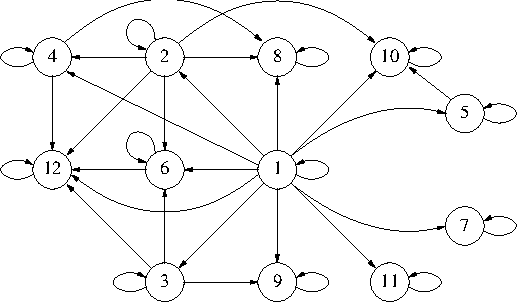
\includegraphics{figures/divisibility.pdf}
\caption{The Digraph for Divisibility on $\set{1,2,\dots,12}$.}
\label{fig:divisibility-digraph}
\end{figure}

%\hfill
%\includegraphics{divi2.pdf}
%{figures/divide12.mps}

\subsection{Paths in Digraphs}

Picturing digraphs with points and arrows makes it natural to talk
about following a \term{path} of successive edges through the graph.
For example, in the digraph of Figure~\ref{fig:divisibility-digraph},
a path might start at vertex 1, successively follow the edges from
vertex 1 to vertex 2, from 2 to 4, from 4 to 12, and then from 12 to
12 twice (or as many times as you like).  We can represent the path
with the sequence of sucessive vertices it went through, in this case:
\[
1,2,4,12,12,12.
\]
So a path is just a sequence of vertices, with consecutive vertices on
the path connected by directed edges.  Here is a formal
definition:

\begin{definition}\label{def:digraph-paths}
A \emph{path in a digraph} is a sequence of vertices $a_0,\dots,a_k$
with $k \ge 0$ such that $\diredge{a_i}{a_{i+1}}$ is an edge of the
digraph for $i = 0,1,\dots, k-1$.  The path is said to \emph{start} at
$a_0$, to \emph{end} at $a_k$, and the \emph{length} of the path is
defined to be $k$.  The path is \emph{simple} iff all the $a_i$'s are
different, that is, if $i \neq j$, then $a_i \neq a_j$.
\end{definition}
Note that a single vertex counts as length zero path that begins and
ends at itself.

It's pretty natural to talk about the edges in a path, but
technically, paths only have points, not edges.  So to instead, we'll
say a path \term{traverses} an edge $\diredge{a}{b}$ when $a$ and $b$
are consecutive vertices in the path.

For any digraph, $R$, we can define some new relations on vertices
based on paths, namely, the \emph{path relation}, $R^*$, and the
\emph{positive-length path relation}, $R^+$:
\begin{align*}
a \mrel{R^*} b &\eqdef \mbox{there is a path in $R$ from $a$ to $b$},\\
a \mrel{R^+} b &\eqdef \mbox{there is a positive length path in $R$ from $a$ to $b$}.
\end{align*}

By the definition of path, both $R^*$ and $R^+$ are transitive.  Since
edges count as length one paths, the edges of $R^+$ include all the
edges of $R$.  The edges of $R^*$ in turn include all the edges of
$R^+$ and, in addition include an edge (self-loop) from each vertex to
itself.  The self-loops get included in $R^*$ because of the a length
zero paths in $R$.  So $R^*$ is reflexive.  \footnote{In many texts,
  $R^+$ is called the \term{transitive closure} and $R^*$ is called
  the \term{reflexive transitive closure} of $R$.}

\section{Picturing Relational Properties}

Many of the relational properties we've discussed have natural
descriptions in terms of paths.  For example:
\begin{description}

\item[Reflexivity:] All vertices have self-loops (a \emph{self-loop} at a
vertex is an arrow going from the vertex back to itself).

\item[Irreflexivity:] No vertices have self-loops.

\item[Antisymmetry:] At most one (directed) edge between different
  vertices.

\item[Asymmetry:] No self-loops and at most one (directed) edge
  between different vertices.

\item[Transitivity:] Short-circuits---for any path through the graph,
there is an arrow from the first vertex to the last vertex on the path.

\item[Symmetry:] A binary relation $R$ is
  \hyperdef{graphs}{symmetric}{\term{symmetric}} iff $aRb$ implies
  $bRa$ for all $a,b$ in the domain of $R$.  That is, if there is an
  edge from $a$ to $b$, there is also one in the reverse direction.
  \begin{editingnotes}
  The pair of directed edges between two vertices may be
  represented by a single \idx{undirected edge} may as well be
  represented without arrows, indicating that they can be followed in
  either direction.
\end{editingnotes}

\end{description}

\section{Composition of Relations}\label{relation_compose_subsec}

There is a simple way to extend \idx{composition} of functions to
composition of relations, and this gives another way to talk about
paths in digraphs.

Let $R: B\to C$ and $S: A \to B$ be relations.  Then the
\idx{composition} of $R$ with $S$ is the binary relation $(R \compose
S): A\to C$ defined by the rule
\[
a \mrel{(R \compose S)} c \eqdef\ \exists b \in B.\, (b \mrel{R} c)
\QAND (a \mrel{S} b).
\]
This agrees with the Definition~\ref{func_compose_def} of composition
in the special case when $R$ and $S$ are functions.
\begin{editingnotes}

\footnote{Some texts define $R \compose S$ the other way around, that
  is, with $S$ applied to the result of applying $R$ first.}

\end{editingnotes}

Now when $R$ is a digraph, it makes sense to compose $R$ with itself.
Then if we let $R^n$ denote the composition of $R$ with itself $n$
times, it's easy to check that $R^n$ is the length-$n$ path relation:
\[
a  \mrel{R^n} b \qiff \mbox{ there is a length $n$ path in $R$ from $a$ to $b$}.
\]
This even works for $n=0$, if we adopt the convention that $R^0$ is
the identity relation $\ident{A}$ on the set, $A$, of vertices.  That
is, $(a \mrel{\ident{A}} b)$ iff $a = b$.

\section{Directed Acyclic Graphs}\label{sec:dag}

\begin{definition}
A \term{cycle} in a digraph is defined by a path that begins and ends
at the same vertex.  This includes the cycle of length zero that
begins and ends at the vertex.  A \term{directed acyclic graph (DAG)}
is a directed graph with no \emph{positive} length cycles.

A \term{simple cycle} in a digraph is a cycle whose vertices are distinct
except for the beginning and end vertices.
\end{definition}

\begin{editingnotes}

In contrast to undirected graphs, a single vertex \emph{is} considered to
be a simple cycle.

\end{editingnotes}

DAG's can be an economical way to represent partial orders.  For
example, in Section~\ref{prereq_sec} the \emph{direct prerequisite}
relation between MIT subjects was used to determine the partial order
of indirect prerequisites on subjects.  This indirect prerequisite
partial order is precisely the positive length path relation of the
direct prerequisites.

\begin{lemma}
If $D$ is a DAG, then $D^+$ is a strict partial order.
\end{lemma}

\begin{proof}
We know that $D^+$ is transitive.  Also, a positive length path from a
vertex to itself would be a cycle, so there are no such paths.  This means
$D^+$ is irreflexive, which implies it is a strict partial order (see
problem~\ref{CP_strict_PO_irreflexive}).
\end{proof}

It's easy to check that conversely, the graph of any strict partial
order is a DAG.

The divisibility partial order can also be more economically represented by
the path relation in a DAG.  \hyperdef{divisibility}{DAG}{A DAG whose
\emph{path} relation is divisibility} on $\set{1,2,\dots,12}$ is shown in
Figure~\ref{fig:divisibility-DAG}; the arrowheads are omitted in the
Figure, and edges are understood to point upwards.

\begin{figure}[h]
%\centering \includegraphics{figures/divi2.pdf}
\begin{center}
\setlength{\unitlength}{1973sp}%
%
\begingroup\makeatletter\ifx\SetFigFont\undefined%
\gdef\SetFigFont#1#2#3#4#5{%
  \reset@font\fontsize{#1}{#2pt}%
  \fontfamily{#3}\fontseries{#4}\fontshape{#5}%
  \selectfont}%
\fi\endgroup%
\begin{picture}(5452,6034)(10475,-13269)
{\color[rgb]{0,0,0}\thinlines
\put(13210,-12952){\circle{618}}
}%
\put(13210,-13027){\makebox(0,0)[b]{\smash{{\SetFigFont{12}{24.0}{\rmdefault}{\mddefault}{\updefault}{\color[rgb]{0,0,0}1}%
}}}}
{\color[rgb]{0,0,0}\put(13192,-9352){\circle{618}}
}%
\put(13192,-9427){\makebox(0,0)[b]{\smash{{\SetFigFont{12}{24.0}{\rmdefault}{\mddefault}{\updefault}{\color[rgb]{0,0,0}4}%
}}}}
{\color[rgb]{0,0,0}\put(13192,-7552){\circle{618}}
}%
\put(13192,-7627){\makebox(0,0)[b]{\smash{{\SetFigFont{12}{24.0}{\rmdefault}{\mddefault}{\updefault}{\color[rgb]{0,0,0}8}%
}}}}
{\color[rgb]{0,0,0}\put(14410,-11170){\circle{618}}
}%
\put(14410,-11245){\makebox(0,0)[b]{\smash{{\SetFigFont{12}{24.0}{\rmdefault}{\mddefault}{\updefault}{\color[rgb]{0,0,0}5}%
}}}}
{\color[rgb]{0,0,0}\put(13810,-10252){\circle{618}}
}%
\put(13810,-10327){\makebox(0,0)[b]{\smash{{\SetFigFont{12}{24.0}{\rmdefault}{\mddefault}{\updefault}{\color[rgb]{0,0,0}10}%
}}}}
{\color[rgb]{0,0,0}\put(12592,-10252){\circle{618}}
}%
\put(12592,-10327){\makebox(0,0)[b]{\smash{{\SetFigFont{12}{24.0}{\rmdefault}{\mddefault}{\updefault}{\color[rgb]{0,0,0}6}%
}}}}
{\color[rgb]{0,0,0}\put(11992,-11170){\circle{618}}
}%
\put(11992,-11245){\makebox(0,0)[b]{\smash{{\SetFigFont{12}{24.0}{\rmdefault}{\mddefault}{\updefault}{\color[rgb]{0,0,0}3}%
}}}}
{\color[rgb]{0,0,0}\put(12592,-8452){\circle{618}}
}%
\put(12592,-8527){\makebox(0,0)[b]{\smash{{\SetFigFont{12}{24.0}{\rmdefault}{\mddefault}{\updefault}{\color[rgb]{0,0,0}12}%
}}}}
{\color[rgb]{0,0,0}\put(15610,-11152){\circle{618}}
}%
\put(15610,-11227){\makebox(0,0)[b]{\smash{{\SetFigFont{12}{24.0}{\rmdefault}{\mddefault}{\updefault}{\color[rgb]{0,0,0}7}%
}}}}
{\color[rgb]{0,0,0}\put(10792,-11170){\circle{618}}
}%
\put(10792,-11245){\makebox(0,0)[b]{\smash{{\SetFigFont{12}{24.0}{\rmdefault}{\mddefault}{\updefault}{\color[rgb]{0,0,0}11}%
}}}}
{\color[rgb]{0,0,0}\put(11992,-9370){\circle{618}}
}%
\put(11992,-9445){\makebox(0,0)[b]{\smash{{\SetFigFont{12}{24.0}{\rmdefault}{\mddefault}{\updefault}{\color[rgb]{0,0,0}9}%
}}}}
{\color[rgb]{0,0,0}\put(13210,-11152){\circle{618}}
}%
\put(13210,-11227){\makebox(0,0)[b]{\smash{{\SetFigFont{12}{24.0}{\rmdefault}{\mddefault}{\updefault}{\color[rgb]{0,0,0}2}%
}}}}
{\color[rgb]{0,0,0}\put(13201,-12661){\line( 0, 1){1200}}
}%
{\color[rgb]{0,0,0}\put(13201,-10861){\line( 0, 1){1200}}
}%
{\color[rgb]{0,0,0}\put(13201,-9061){\line( 0, 1){1200}}
}%
{\color[rgb]{0,0,0}\put(13201,-9061){\line( 0, 1){1200}}
}%
{\color[rgb]{0,0,0}\put(12601,-9961){\line( 0, 1){1200}}
}%
{\color[rgb]{0,0,0}\put(12001,-10861){\line( 0, 1){1200}}
}%
{\color[rgb]{0,0,0}\put(12901,-11161){\makebox(3.3333,23.3333){\SetFigFont{5}{6}{\rmdefault}{\mddefault}{\updefault}.}}
}%
{\color[rgb]{0,0,0}\multiput(14251,-10910)(-10.28143,13.70857){29}{\makebox(3.3333,23.3333){\SetFigFont{5}{6}{\rmdefault}{\mddefault}{\updefault}.}}
}%
{\color[rgb]{0,0,0}\multiput(13009,-10914)(-10.28143,13.70857){29}{\makebox(3.3333,23.3333){\SetFigFont{5}{6}{\rmdefault}{\mddefault}{\updefault}.}}
}%
{\color[rgb]{0,0,0}\multiput(13028,-9107)(-10.28143,13.70857){29}{\makebox(3.3333,23.3333){\SetFigFont{5}{6}{\rmdefault}{\mddefault}{\updefault}.}}
}%
{\color[rgb]{0,0,0}\multiput(12168,-10904)(10.28143,13.70857){29}{\makebox(3.3333,23.3333){\SetFigFont{5}{6}{\rmdefault}{\mddefault}{\updefault}.}}
}%
{\color[rgb]{0,0,0}\multiput(13387,-10884)(10.28143,13.70857){29}{\makebox(3.3333,23.3333){\SetFigFont{5}{6}{\rmdefault}{\mddefault}{\updefault}.}}
}%
{\color[rgb]{0,0,0}\put(13017,-12714){\line(-2, 3){861.692}}
}%
{\color[rgb]{0,0,0}\put(12915,-12863){\line(-4, 3){1943.360}}
}%
{\color[rgb]{0,0,0}\put(13425,-12739){\line( 2, 3){861.692}}
}%
{\color[rgb]{0,0,0}\put(13517,-12849){\line( 4, 3){1943.360}}
}%
\end{picture}%

\end{center}
\caption{A DAG whose Path Relation is Divisibility on $\set{1,2,\dots,12}$.}
\label{fig:divisibility-DAG}
\end{figure}

If we're using a DAG to represent a partial order ---so all we care
about is the the path relation of the DAG ---we could replace the DAG
with any other DAG with the same path relation.  This raises the
question of finding a DAG with the same path relation but the
\emph{smallest} number of edges.  This DAG turns out to be unique and
easy to find (see Problem~\ref{CP_covering_edges}).

\begin{problems}
\practiceproblems
\pinput{TP_strictPOs_are_DAGs}

\classproblems
\pinput{CP_covering_edges}

\homeworkproblems
\pinput{PS_path_relation_composition}
\pinput{PS_finite_transitive_closure}
\end{problems}

\begin{editingnotes}
* add problem using matrix operations to compute transitive closure

* add section on shortest paths?

* add section on directed tours and walks?
\end{editingnotes}

%\chapter{Communication Networks}\label{comm_net_chap}

\hyperdef{communication}{networks}{\section{Communication
    Networks}}\label{comm_net_sec}

\begin{editingnoes}
ADD DISCUSSION of routing problems in general, with defs of

*``IO-assignments'' = specification of sources & destinations of
packets,

* ``routing'' = paths that achieve the IO-assignment,

* congestion and latency of a routing.

* Possible latency/congestion tradeoffs

* congestion and latency of a net.
\end{editingnotes}


Modeling communication networks is an important application of
digraphs in computer science.  In this such models, vertices represent
computers, processors, and switches; edges will represent wires,
fiber, or other transmission lines through which data flows.  For some
communication networks, like the internet, the corresponding graph is
enormous and largely chaotic.  Highly structured networks, by
contrast, find application in telephone switching systems and the
communication hardware inside parallel computers.  In this chapter,
we'll look at some of the nicest and most commonly used structured
networks.

\section{Complete Binary Tree}

Let's start with a \term{complete binary tree}.  Here is an example
with 4 inputs and 4 outputs.

\mfigure{!}{2.5in}{figures/bintree-notes}

The kinds of communication networks we consider aim to transmit packets of
data between computers, processors, telephones, or other devices.  The
term \term{packet} refers to some roughly fixed-size quantity of data---
256 bytes or 4096 bytes or whatever.  In this diagram and many that
follow, the squares represent \term{terminals}, sources and destinations
for packets of data.  The circles represent \term{switches}, which direct
packets through the network.  A switch receives packets on incoming edges
and relays them forward along the outgoing edges.  Thus, you can imagine a
data packet hopping through the network from an input terminal, through a
sequence of switches joined by directed edges, to an output terminal.

Recall that there is a unique simple path between every pair of vertices
in a tree.  So the natural way to route a packet of data from an input
terminal to an output in the complete binary tree is along the
corresponding directed path.  For example, the route of a packet traveling
from input 1 to output 3 is shown in bold.

\section{Routing Problems}

Communication networks are supposed to get packets from inputs to outputs,
with each packet entering the network at its own input switch and arriving
at its own output switch.  We're going to consider several different
communication network designs, where each network has $N$ inputs and
$N$ outputs; for convenience, we'll assume $N$ is a power of two.

Which input is supposed to go where is specified by a permutation of
$\set{0, 1, \dots, N - 1}$.  So a permutation, $\pi$, defines a \term{
  routing problem}: get a packet that starts at input $i$ to output
$\pi(i)$.  A \term{routing}, $P$, that \term{solves} a routing problem,
$\pi$, is a set of paths from each input to its specified output.  That
is, $P$ is a set of $n$ paths, $P_i$, for $i=0\dots,N-1$, where $P_i$ goes
from input $i$ to output $\pi(i)$.

\section{Network Diameter}

The delay between the time that a packets arrives at an input and arrives
at its designated output is a critical issue in communication networks.
Generally this delay is proportional to the length of the path a packet
follows.  Assuming it takes one time unit to travel across a wire,
\begin{editingnotes}
and that there are no additional delays at switches,
\end{editingnotes}
the delay of a packet will be the number of wires it crosses going from
input to output.

\begin{editingnotes}

\footnote{Latency is often measured as the number of switches that
a packet must pass through when traveling between the most distant input
and output, since switches usually have the biggest impact on network
speed.  For example, in the complete binary tree example, the packet
traveling from input 1 to output 3 crosses 5 switches.}

\end{editingnotes}

Generally packets are routed to go from input to output by the shortest
path possible.  With a shortest path routing, the worst case delay is the
distance between the input and output that are farthest apart.  This is
called the \term{diameter} of the network.  In other words, the diameter
of a network\footnote{The usual definition of \emph{diameter} for a
general \textit{graph} (simple or directed) is the largest distance
between \emph{any} two vertices, but in the context of a communication
network we're only interested in the distance between inputs and outputs,
not between arbitrary pairs of vertices.} is the maximum length of any
shortest path between an input and an output.  For example, in the
complete binary tree above, the distance from input 1 to output 3 is six.
No input and output are farther apart than this, so the diameter of this
tree is also six.

More generally, the diameter of a complete binary tree with $N$ inputs and
outputs is $2 \log N + 2$.  (All logarithms in this lecture--- and in most
of computer science ---are base 2.)  This is quite good, because the
logarithm function grows very slowly.  We could connect up $2^{10} = 1024$
inputs and outputs using a complete binary tree and the worst input-output
delay for any packet would be this diameter, namely, $2 \log(2^{10}) + 2 =
22$.

\subsection{Switch Size}

One way to reduce the diameter of a network is to use larger switches.
For example, in the complete binary tree, most of the switches have
three incoming edges and three outgoing edges, which makes them $3
\times 3$ switches.  If we had $4 \times 4$ switches, then we could
construct a complete \textit{ternary} tree with an even smaller
diameter.  In principle, we could even connect up all the inputs and
outputs via a single monster $N \times N$ switch.

\begin{editingnotes}
\mfigure{!}{1in}{figures/monster-switch}
\end{editingnotes}

This isn't very productive, however, since we've just concealed the
original network design problem inside this abstract switch.
Eventually, we'll have to design the internals of the monster switch
using simpler components, and then we're right back where we started.
So the challenge in designing a communication network is figuring out
how to get the functionality of an $N \times N$ switch using
fixed size, elementary devices, like $3 \times 3$ switches.
\begin{solution}
Following this approach, we can build arbitrarily large networks
just by adding in more building blocks. 
\end{solution}

\section{Switch Count}

Another goal in designing a communication network is to use as few
switches as possible.  The number of switches in a complete binary tree is
$1 + 2 + 4 + 8 + \cdots + N$, since there is 1 switch at the top (the
``root switch''), 2 below it, 4 below those, and so forth.  By the
formula~\eqref{geometric-n} for geometric sums, the total number of
switches is $2 N - 1$, which is nearly the best possible with $3 \times 3$
switches.

\section{Network  Latency}

We'll sometimes be choosing routings through a network that optimize some
quantity besides delay.  For example, in the next section we'll be trying
to minimize packet congestion.  When we're not minimizing delay, shortest
routings are not always the best, and in general, the delay of a packet
will depend on how it is routed.  For any routing, the most delayed packet
will be the one that follows the longest path in the routing.  The length
of the longest path in a routing is called its \term{latency}.

%NEEDS REVISION:

The latency of a \emph{network} depends on what's being optimized.  It is
measured by assuming that optimal routings are always chosen in getting
inputs to their specified outputs.  That is, for each routing problem,
$\pi$, we choose an optimal routing that solves $\pi$.  Then \term{network
  latency} is defined to be the largest routing latency among these
optimal routings.  Network latency will equal network diameter if routings
are always chosen to optimize delay, but it may be significantly larger if
routings are chosen to optimize something else.

For the networks we consider below, paths from input to output are
uniquely determined (in the case of the tree) or all paths are the same
length, so network latency will always equal network diameter.


\section{Congestion}

The complete binary tree has a fatal drawback: the root switch is a
bottleneck.  At best, this switch must handle an enormous amount of
traffic: every packet traveling from the left side of the network to the
right or vice-versa.  Passing all these packets through a single switch
could take a long time.  At worst, if this switch fails, the network is
broken into two equal-sized pieces.

For example, if the routing problem is given by the identity permutation,
$\ident{}(i) \eqdef i$, then there is an easy routing, $P$, that solves
the problem: let $P_i$ be the path from input $i$ up through one switch
and back down to output $i$.  On the other hand, if the problem was given
by $\pi(i) \eqdef (N - 1) - i$, then in \emph{any} solution, $Q$, for
$\pi$, each path $Q_i$ beginning at input $i$ must eventually loop all
the way up through the root switch and then travel back down to output $(N
- 1) - i$.  These two situations are illustrated below.

\mfigure{!}{1,5in}{figures/bintree2}

We can distinguish between a ``good'' set of paths and a ``bad'' set based
on congestion.  The \term{congestion} of a routing, $P$, is equal to the
largest number of paths in $P$ that pass through a single switch.  For
example, the congestion of the routing on the left is 1, since at most 1
path passes through each switch.  However, the congestion of the routing
on the right is 4, since 4 paths pass through the root switch (and the two
switches directly below the root).  Generally, lower congestion is better
since packets can be delayed at an overloaded switch.

By extending the notion of congestion to networks, we can also distinguish
between ``good'' and ``bad'' networks with respect to bottleneck problems.
For each routing problem, $\pi$, for the network, we assume a routing is
chosen that optimizes congestion, that is, that has the minimum congestion
among all routings that solve $\pi$.  Then the largest congestion that
will ever be suffered by a switch will be the maximum congestion among
these optimal routings.  This ``maximin'' congestion is called the
\term{congestion of the network}.

\begin{editingnotes}

You may find it helpful to think about max congestion in terms of a value
game.  You design your spiffy, new communication network; this defines the
game.  Your opponent makes the first move in the game: she inspects your
network and specifies a permutation routing problem that will strain your
network.\iffalse
That is, her first move is a specification of which input terminals must
send a packet to which output terminals.
\fi
You move second: given her specification, you choose the precise paths
that the packets should take through your network; you're trying to avoid
overloading any one switch.  Then her next move is to pick a switch with
as large as possible a number of packets passing through it; this number
is her score in the competition.  The max congestion of your network is
the largest score she can ensure; in other words, it is precisely the
max-value of this game.

For example, if your enemy were trying to defeat the complete binary
tree, she would choose a permutation like $\pi(i) = (N - 1) - i$.
Then for \textit{every} packet $i$, you would be forced to select a
path $P_{i, \pi(i)}$ passing through the root switch.  Thus, the max
congestion of the complete binary tree is $N$--- which is horrible!

\end{editingnotes}

So for the complete binary tree, the worst permutation would be $\pi(i)
\eqdef (N - 1) - i$.  Then in every possible solution for $\pi$,
\textit{every} packet, would have to follow a path passing through the
root switch.  Thus, the max congestion of the complete binary tree is $N$
---which is horrible!

Let's tally the results of our analysis so far:
%
\[
\begin{array}{r|c|c|c|c}
\textbf{network} &
\textbf{diameter} &
\textbf{switch size} &
\textbf{\# switches} &
\textbf{congestion} \\ \hline
\text{complete binary tree} & 2 \log N + 2 & 3 \times 3 & 2N - 1 & N \\
\end{array}
\]

\hyperdef{2-D}{array}{\section{2-D Array}}\label{2Darray}

Let's look at an another communication network.  This one is called a
\term{2-dimensional array} or \term{grid}.

\begin{editingnotes}
or \term{crossbar}.
\end{editingnotes}

\mfigure{!}{2in}{figures/grid}

Here there are four inputs and four outputs, so $N = 4$.

The diameter in this example is 8, which is the number of edges between
input 0 and output 3.  More generally, the diameter of an array with $N$
inputs and outputs is $2N$, which is much worse than the diameter of $2
\log N + 2$ in the complete binary tree.  On the other hand, replacing a
complete binary tree with an array almost eliminates congestion.

\begin{theorem}
The congestion of an $N$-input array is 2.
\end{theorem}

\begin{proof}
First, we show that the congestion is at most 2.  Let $\pi$ be any
permutation.  Define a solution, $P$, for $\pi$ to be the set of paths,
$P_i$, where $P_i$ goes to the right from input $i$ to column $\pi(i)$ and
then goes down to output $\pi(i)$.  Thus, the switch in row $i$ and column
$j$ transmits at most two packets: the packet originating at input
$i$ and the packet destined for output $j$.

Next, we show that the congestion is at least 2.  This follows because in
any routing problem, $\pi$, where $\pi(0) = 0$ and $\pi(N-1) =
N-1$, two packets must pass through the lower left switch.
\end{proof}

As with the tree, the network latency when minimizing congestion is the
same as the diameter.  That's because all the paths between a given input
and output are the same length.

Now we can record the characteristics of the 2-D array.
%
\[
\begin{array}{r|c|c|c|c}
\textbf{network} &
\textbf{diameter} &
\textbf{switch size} &
\textbf{\# switches} &
\textbf{congestion} \\ \hline
\text{complete binary tree} & 2 \log N + 2 & 3 \times 3 & 2N - 1 & N \\
\text{2-D array} & 2 N & 2 \times 2 & N^2 & 2
\end{array}
\]
%
The crucial entry here is the number of switches, which is $N^2$.
This is a major defect of the 2-D array; a network of size $N = 1000$
would require a \textit{million} $2 \times 2$ switches!  Still, for
applications where $N$ is small, the simplicity and low congestion of
the array make it an attractive choice.


\section{Butterfly}

The Holy Grail of switching networks would combine the best properties
of the complete binary tree (low diameter, few switches) and of the
array (low congestion).  The \term{butterfly} is a widely-used
compromise between the two.  \iffalse
Here is a butterfly network with $N = 8$
inputs and outputs.

\mfigure{!}{3.0in}{figures/butterfly2}

The structure of the butterfly is certainly more complicated than that
of the complete binary tree or 2-D array!  Let's work through the
various parts of the butterfly.

All the terminals and switches in the network are arranged in $N$
rows.  In particular, input $i$ is at the left end of row $i$, and
output $i$ is at the right end of row $i$.  Now let's label the rows
in $\textit{binary}$; thus, the label on row $i$ is the binary number
$b_1 b_2 \dots b_{\log N}$ that represents the integer $i$.

Between the inputs and the outputs, there are $\log(N) + 1$ levels of
switches, numbered from 0 to $\log N$.  Each level consists of a
column of $N$ switches, one per row.  Thus, each switch in the network
is uniquely identified by a sequence $(b_1, b_2, \dots, b_{\log N},
l)$, where $b_1 b_2 \dots b_{\log N}$ is the switch's row in binary
and $l$ is the switch's level.

All that remains is to describe how the switches are connected up.
The basic connection pattern is expressed below in a compact notation:
%
\[
(b_1, b_2, \dots, b_{l+1}, \dots, b_{\log N}, l)
\begin{array}{l}
\nearrow \\
\searrow
\end{array}
\begin{array}{l}
(b_1, b_2, \dots, b_{l+1}, \dots, b_{\log N}, l + 1) \\
\\
(b_1, b_2, \dots, \overline{b_{l+1}}, \dots, b_{\log N}, l + 1)
\end{array}
\]
%
This says that there are directed edges from switch $(b_1, b_2,
\dots, b_{\log N}, l)$ to two switches in the next level.  One edge
leads to the switch in the \textit{same} row, and the other edge leads
to the switch in the row obtained by \textit{inverting} bit $l + 1$.
For example, referring back to the illustration of the size $N = 8$
butterfly, there is an edge from switch $(0, 0, 0, 0)$ to switch $(0,
0, 0, 1)$, which is in the same row, and to switch $(1, 0, 0, 1)$,
which is the row obtained by inverting bit $l + 1 = 1$.
\fi

A good way to understand butterfly networks is as a recursive data
type.  The recursive definition works better if we define just the
switches and their connections, omitting the terminals.  So we
recursively define $F_n$ to be the switches and connections of the
butterfly net with $N \eqdef 2^n$ input and output switches.

The base case is $F_1$ with 2 input switches and 2 output switches
connected as in Figure~\ref{fig:butterfly-base}.

\begin{figure}[h]
\begin{center}
\mfigure{!}{2.5in}{figures/butterfly-base}
%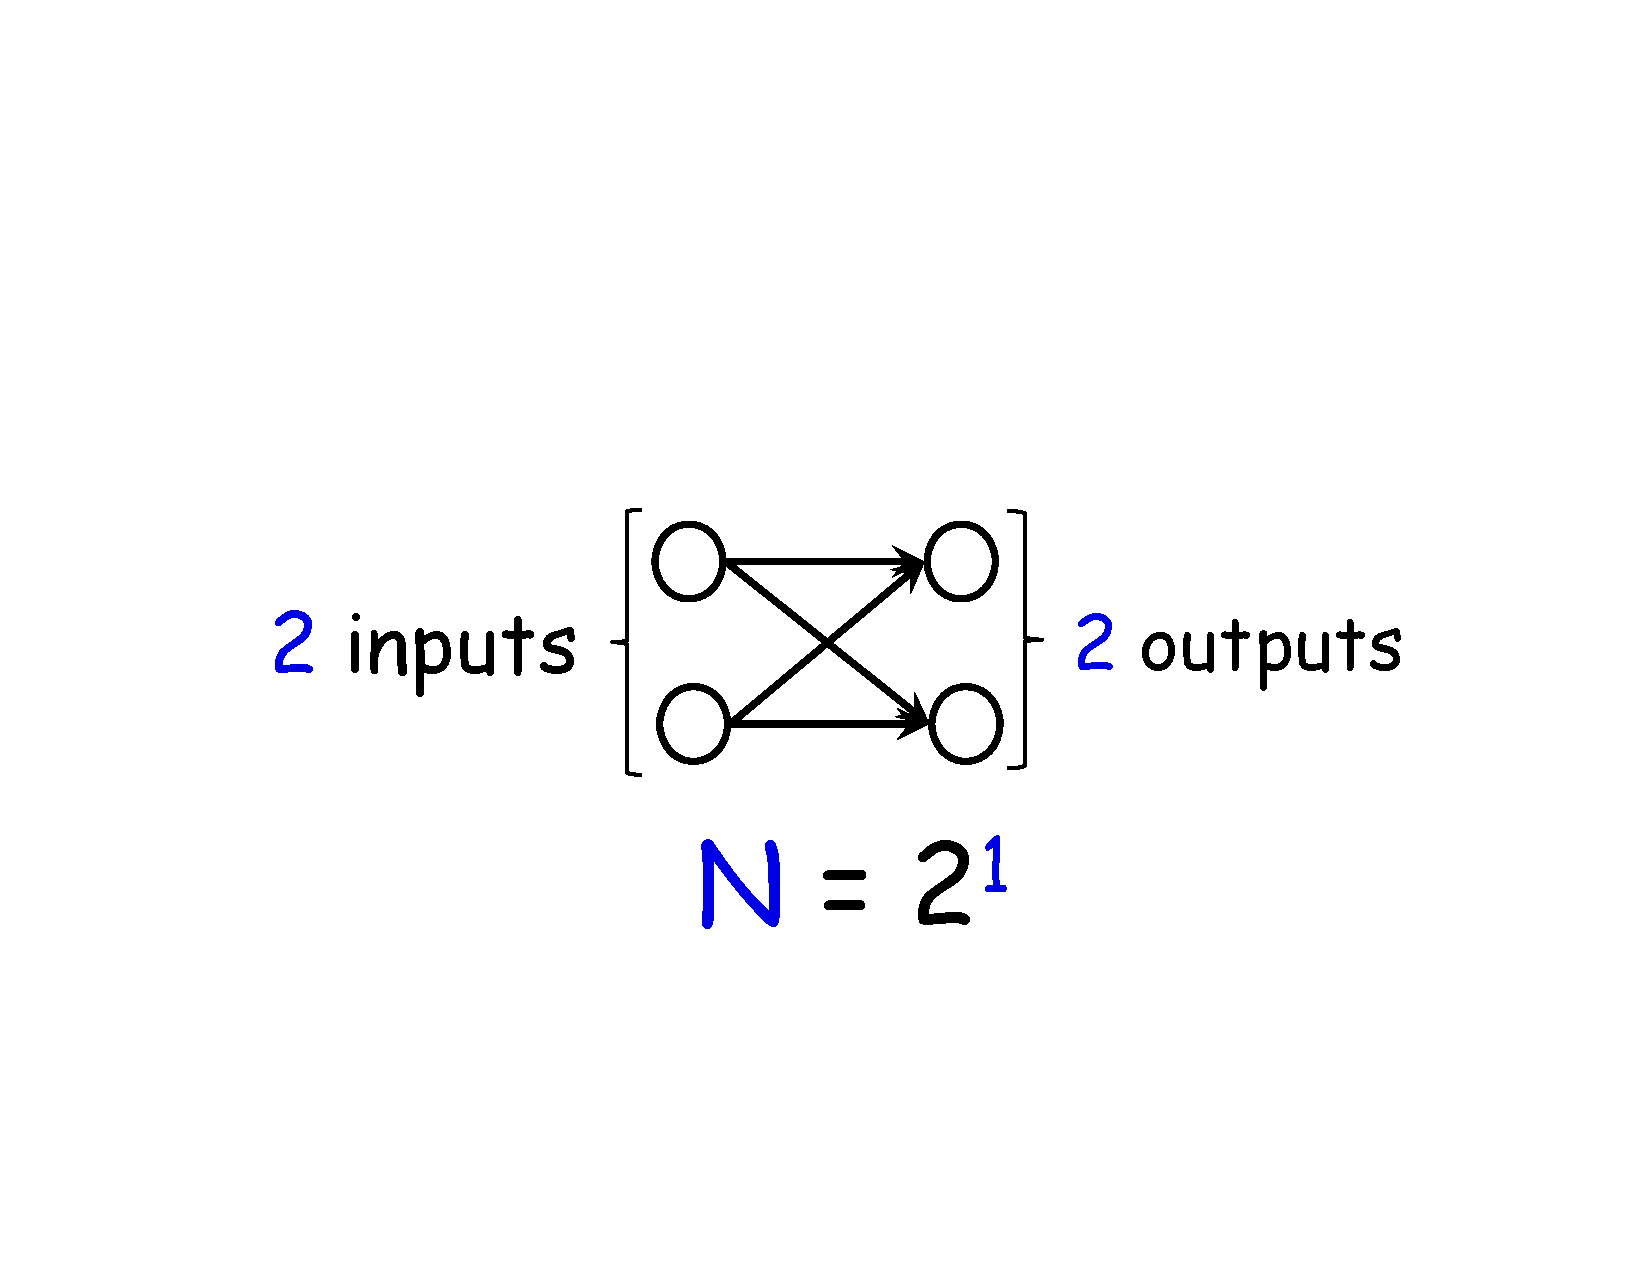
\includegraphics{figures/butterfly-base}
\end{center}
\caption{$F_1$, the Butterfly Net switches with $N=2^1$.}
\label{fig:butterfly-base}
\end{figure}

\begin{editingnotes}

The butterfly of size $2N$ consists of two butterflies of size $N$, which
are shown in dashed boxes below, and one additional level of switches.
Each switch in the new level has directed edges to a pair of
corresponding switches in the smaller butterflies; one example is
dashed in the figure.

\mfigure{!}{3in}{figures/butterfly3}

Despite the relatively complicated structure of the butterfly, there
is a simple way to route packets.  In particular, suppose that we want
to send a packet from input $x_1 x_2 \dots x_{\log N}$ to output $y_1
y_2 \dots y_{\log N}$.  (Here we are specifying the input and output
numbers in binary.)  Roughly, the plan is to ``correct'' the first bit
by level 1, correct the second bit by level 2, and so forth.  Thus,
the sequence of switches visited by the packet is:
%
\begin{align*}
(x_1, x_2, x_3, \dots, x_{\log N}, 0)
    & \to (y_1, x_2, x_3, \dots, x_{\log N}, 1) \\
    & \to (y_1, y_2, x_3, \dots, x_{\log N}, 2) \\
    & \to (y_1, y_2, y_3, \dots, x_{\log N}, 3) \\
    & \to \qquad \dots \\
    & \to (y_1, y_2, y_3, \dots, y_{\log N}, \log N) \\
\end{align*}
%
In fact, this is the \textit{only} path from the input to the output!

\end{editingnotes}

In the constructor step, we construct $F_{n+1}$ with $2^{n+1}$ inputs and
outputs out of two $F_n$ nets connected to a new set of $2^{n+1}$ input
switches, as shown in as in Figure~\ref{fig:butterfly-recursive}.  That
is, the $i$th and $2^n+i$th new input switches are each connected to the
same two switches, namely, to the $i$th input switches of each of two
$F_n$ components for $i=1,\dots,2^n$.  The output switches of $F_{n+1}$
are simply the output switches of each of the $F_n$ copies.

\begin{figure}[h]
\begin{center}
\mfigure{!}{3in}{figures/butterfly-recursive}
%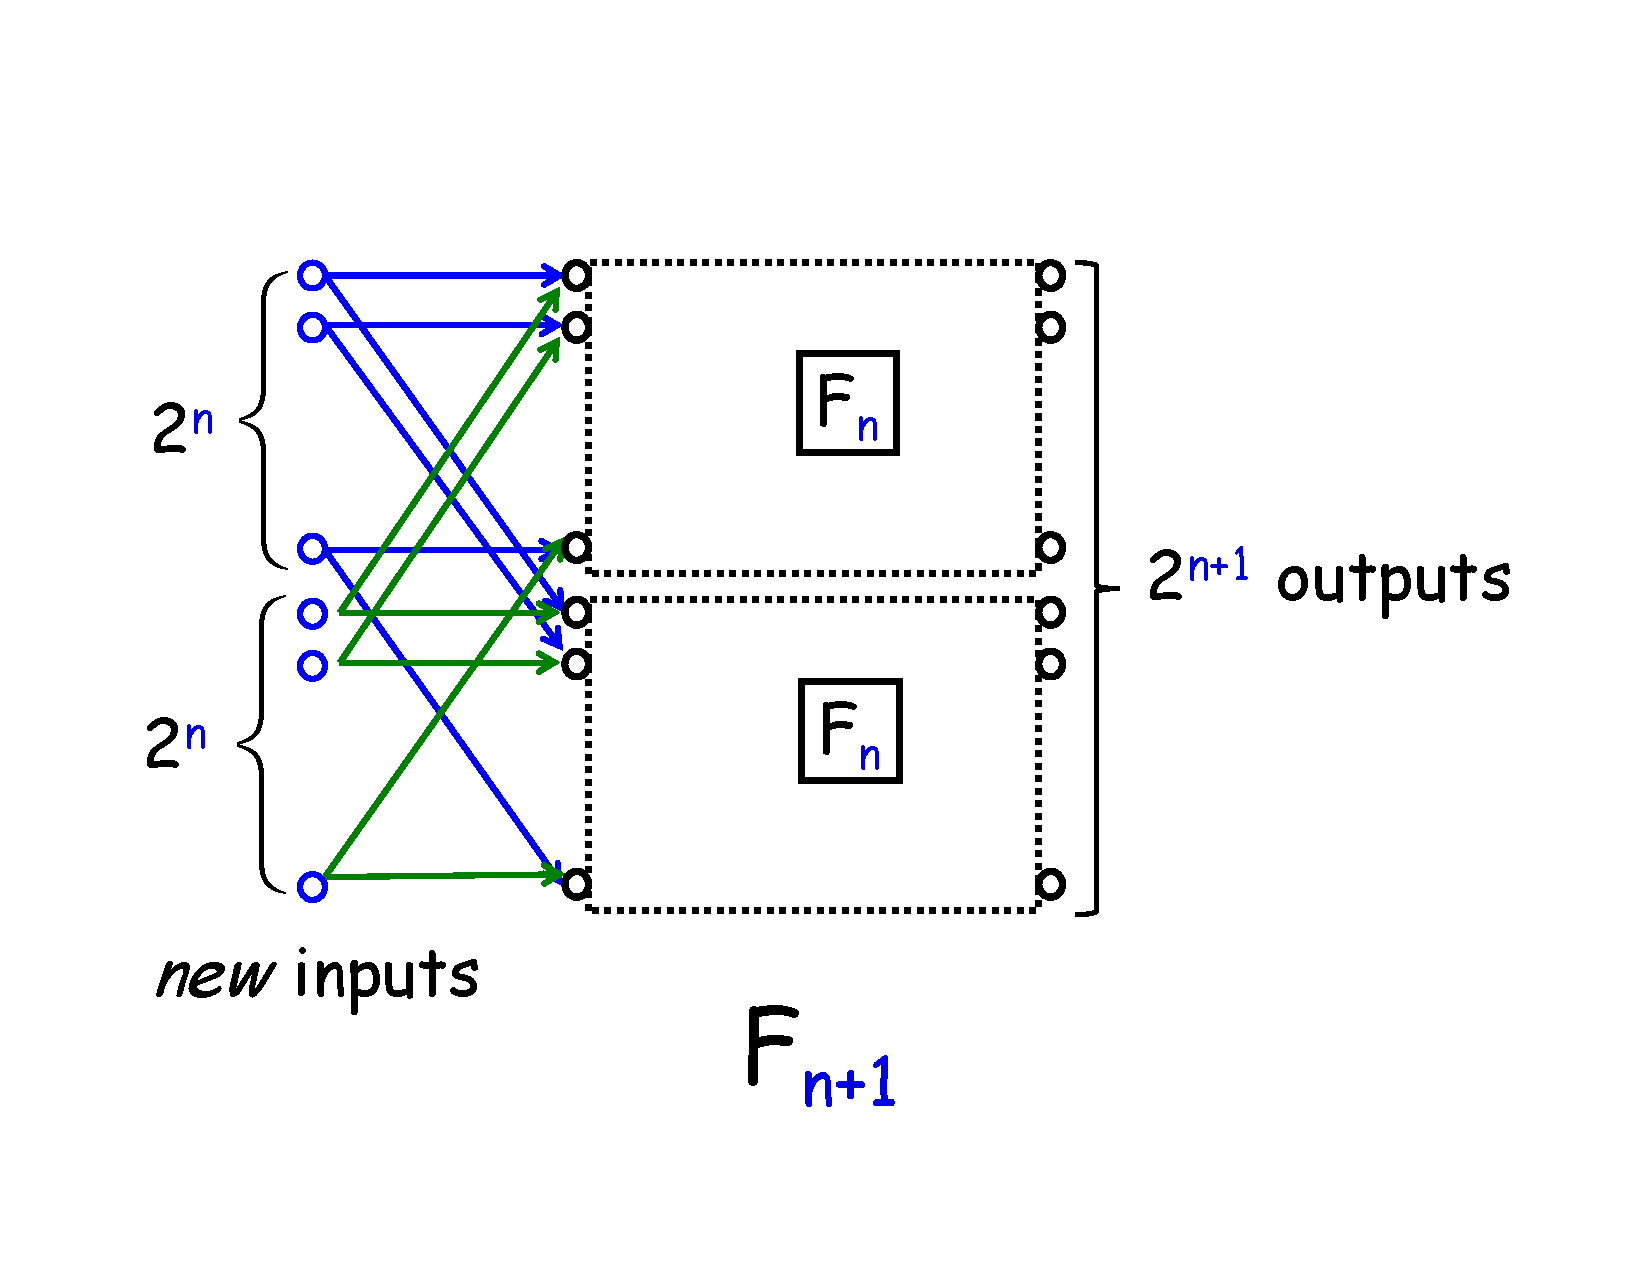
\includegraphics{figures/butterfly-recursive}
\end{center}
\caption{$F_{n+1}$, the Butterfly Net switches with $2^{n+1}$ inputs
and outputs.}
\label{fig:butterfly-recursive}
\end{figure}

So $F_{n+1}$ is laid out in columns of height $2^{n+1}$ by adding one more
column of switches to the columns in $F_n$.  Since the construction starts
with two columns when $n=1$, the $F_{n+1}$ switches are arrayed in $n+1$
columns.  The total number of switches is the height of the columns times
the number of columns, namely, $2^{n+1}(n+1)$.  Remembering that $n=\log
N$, we conclude that the Butterfly Net with $N$ inputs has $N(\log N +1)$
switches.

Since every path in $F_{n+1}$ from an input switch to an output is the
same length, namely, $n+1$, the diameter of the Butterfly net with
$2^{n+1}$ inputs is this length plus two because of the two edges
connecting to the terminals (square boxes) ---one edge from input
terminal to input switch (circle) and one from output switch to output
terminal.

There is an easy recursive procedure to route a packet through the
Butterfly Net.  In the base case, there is obviously only one way to route
a packet from one of the two inputs to one of the two outputs.  Now
suppose we want to route a packet from an input switch to an output switch
in $F_{n+1}$.  If the output switch is in the ``top'' copy of $F_n$, then
the first step in the route must be from the input switch to the unique
switch it is connected to in the top copy; the rest of the route is
determined by recursively routing the rest of the way in the top copy of
$F_n$.  Likewise, if the output switch is in the ``bottom'' copy of $F_n$,
then the first step in the route must be to the switch in the bottom copy,
and the rest of the route is determined by recursively routing in the
bottom copy of $F_n$.  In fact, this argument shows that the routing is
\emph{unique}: there is exactly one path in the Butterfly Net from each
input to each output, which implies that the network latency when
minimizing congestion is the same as the diameter.

The congestion of the butterfly network is about $\sqrt{N}$, more
precisely, the congestion is $\sqrt{N}$ if $N$ is an even power of 2 and
$\sqrt{N/2}$ if $N$ is an odd power of 2.  A simple proof of this appears
in Problem\ref{PS_butterfly_congestion}.

Let's add the butterfly data to our comparison table:
%
\[
\begin{array}{r|c|c|c|c}
\textbf{network} &
\textbf{diameter} &
\textbf{switch size} &
\textbf{\# switches} &
\textbf{congestion} \\ \hline
\text{complete binary tree} & 2 \log N + 2 & 3 \times 3 & 2N - 1 & N \\
\text{2-D array} & 2 N & 2 \times 2 & N^2 & 2 \\
\text{butterfly} & \log N + 2 & 2 \times 2 & N (\log(N) + 1) & \sqrt{N} \text{ or } \sqrt{N/2}
\end{array}
\]
%
The butterfly has lower congestion than the complete binary tree.  And
it uses fewer switches and has lower diameter than the array.
However, the butterfly does not capture the best qualities of each
network, but rather is a compromise somewhere between the two.  So our
quest for the Holy Grail of routing networks goes on.

\section{Bene\u{s} Network}

In the 1960's, a researcher at Bell Labs named Bene\u{s} had a
remarkable idea.  He obtained a marvelous communication network with
congestion 1 by placing \textit{two} butterflies back-to-back.  This
amounts to recursively growing \term{Bene\u{s} nets} by adding both inputs
and outputs at each stage.  Now we recursively define $B_n$ to be the
switches and connections (without the terminals) of the Bene\u{s} net
with $N \eqdef 2^n$ input and output switches.

The base case, $B_1$, with 2 input switches and 2 output switches is
exactly the same as $F_1$ in Figure~\ref{fig:butterfly-base}.

In the constructor step, we construct $B_{n+1}$ out of two $B_n$ nets
connected to a new set of $2^{n+1}$ input switches \emph{and also} a
new set of $2^{n+1}$ output switches.  This is illustrated in
Figure~\ref{fig:benes-recursive}.

Namely, the $i$th and $2^n+i$th new input switches are each connected to
the same two switches, namely, to the $i$th input switches of each of two
$B_n$ components for $i=1,\dots,2^n$, exactly as in the Butterfly net.  In
addition, the $i$th and $2^n+i$th new \emph{output} switches are connected
to the same two switches, namely, to the $i$th output switches of each of
two $B_n$ components.

\begin{figure}[h]
\begin{center}
\mfigure{!}{4in}{figures/benes-recursive}
%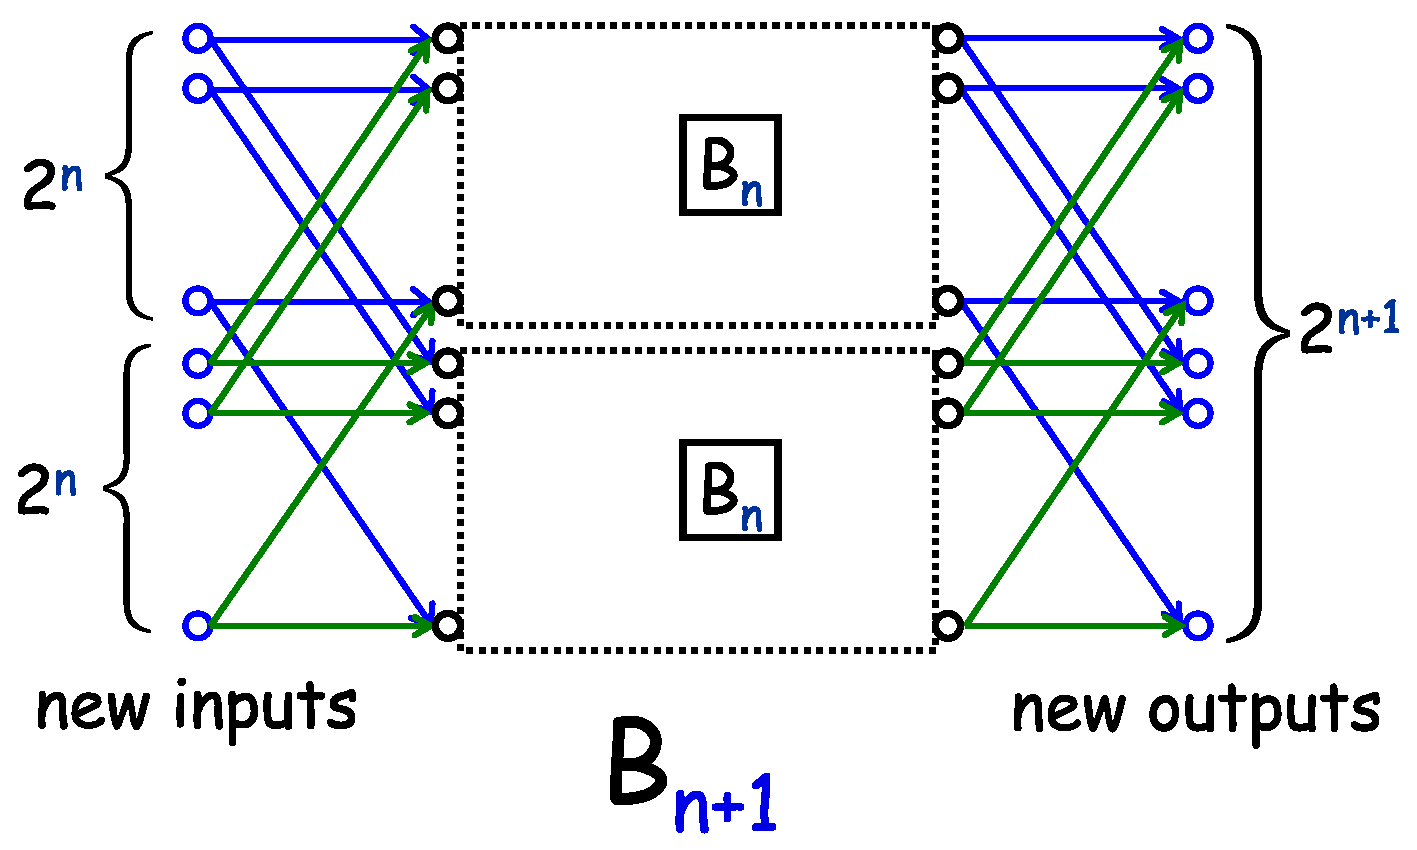
\includegraphics{figures/benes-recursive}
\end{center}
\caption{$B_{n+1}$, the Bene\u{s} Net switches with $2^{n+1}$ inputs
and outputs.}
\label{fig:benes-recursive}
\end{figure}

Now $B_{n+1}$ is laid out in columns of height $2^{n+1}$ by adding two
more columns of switches to the columns in $B_n$.  So the $B_{n+1}$
switches are arrayed in $2(n+1)$ columns.  The total number of
switches is the number of columns times the height of the columns,
namely, $2(n+1)2^{n+1}$.

All paths in $B_{n+1}$ from an input switch to an output are the same
length, namely, $2(n+1)-1$, and the diameter of the Bene\u{s} net with
$2^{n+1}$ inputs is this length plus two because of the two edges
connecting to the terminals.

\begin{editingnotes}

\mfigure{5in}{!}{figures/benes}

% This should make the construction of the 2-colorable graph in the
% congestion proof just a little more apparent.

This network now has levels labeled $0,\dots ,2 \log N + 1$. For $1 \leq k
\leq \log N$, the connections from level $k-1$ to level $k$ are just as in
the Butterfly network, the connections based on bit $k$. The conections
from level $2 \log N - k + 1$ to level $2 \log N - k + 2$ are also the
ones based on bit $k$.  (Informally, to make the connections from level
$0$ to level $2 \log N +1$ one level at a time, use the connections based
on bits $1,2,3,\dots, \log N - 1, \log N, \log N - 1, \log N - 2, \dots,
3,2,1$ in that order.)

\end{editingnotes}

So Bene\u{s} has doubled the number of switches and the diameter, of
course, but completely eliminates congestion problems!  The proof of
this fact relies on a clever induction argument that we'll come to in
a moment.  Let's first see how the Bene\u{s} network stacks up:
%
\[
\begin{array}{r|c|c|c|c}
\textbf{network} &
\textbf{diameter} &
\textbf{switch size} &
\textbf{\# switches} &
\textbf{congestion} \\ \hline
\text{complete binary tree} & 2 \log N + 2 & 3 \times 3 & 2N - 1 & N \\
\text{2-D array} & 2 N & 2 \times 2 & N^2 & 2 \\
\text{butterfly} & \log N + 2 & 2 \times 2 & N (\log(N) + 1) & \sqrt{N} \text{ or } \sqrt{N/2} \\
\text{Bene\u{s}} & 2 \log N + 1 & 2 \times 2 &  2 N \log N & 1
\end{array}
\]
%
The Bene\u{s} network has small size and diameter, and completely
eliminates congestion.  The Holy Grail of routing networks is in hand!

\begin{theorem}
The congestion of the $N$-input Bene\u{s} network is 1.

\iffalse , where $N = 2^a$ for some $a \geq 1$\fi

\end{theorem}

\begin{proof}
By induction on $n$ where $N=2^n$.  So the induction hypothesis is

\[
P(n) \eqdef  \text{the congestion of $B_n$ is 1}.
\]

\textbf{Base case} ($n=1$): $B_1 =F_1$ and the unique routings in $F_1$
have congestion 1.

\textbf{Inductive step}: We assume that the congestion of an $N=2^n$-input
Bene\u{s} network is 1 and prove that the congestion of a $2N$-input
Bene\u{s} network is also 1.

\textbf{Digression. }  Time out!  Let's work through an example,
develop some intuition, and then complete the proof.  In the Bene\u{s}
network shown below with $N=8$ inputs and outputs, the two
4-input/output subnetworks are in dashed boxes.

\mfigure{!}{3in}{figures/benes-decomp}

By the inductive assumption, the subnetworks can each route an
arbitrary permutation with congestion 1.  So if we can guide packets
safely through just the first and last levels, then we can rely on
induction for the rest!  Let's see how this works in an example.
Consider the following permutation routing problem:
%
\begin{align*}
\pi(0) & = 1 & \pi(4) & = 3 \\
\pi(1) & = 5 & \pi(5) & = 6 \\
\pi(2) & = 4 & \pi(6) & = 0 \\
\pi(3) & = 7 & \pi(7) & = 2
\end{align*}

We can route each packet to its destination through either the upper
subnetwork or the lower subnetwork.  However, the choice for one
packet may constrain the choice for another.  For example, we can not
route both packet 0 \textit{and} packet 4 through the same network
since that would cause two packets to collide at a single switch,
resulting in congestion.  So one packet must go through the upper
network and the other through the lower network.  Similarly, packets 1
and 5, 2 and 6, and 3 and 7 must be routed through different networks.
Let's record these constraints in a graph.  The vertices are the 8
packets.  If two packets must pass through different networks, then
there is an edge between them.  Thus, our constraint graph looks like
this:

\mfigure{!}{1.5in}{figures/benes-const1}

Notice that at most one edge is incident to each vertex.

The output side of the network imposes some further constraints.  For
example, the packet destined for output 0 (which is packet 6) and the
packet destined for output 4 (which is packet 2) can not both pass
through the same network; that would require both packets to arrive
from the same switch.  Similarly, the packets destined for outputs 1
and 5, 2 and 6, and 3 and 7 must also pass through different switches.
We can record these additional constraints in our graph with gray
edges:

\mfigure{!}{1.5in}{figures/benes-const2}

Notice that at most one new edge is incident to each vertex.
The two lines drawn between vertices 2 and 6 reflect the two different
reasons why these packets must be routed through different networks.
However, we intend this to be a simple graph; the two lines still
signify a single edge.

Now here's the key insight: \textit{a 2-coloring of the graph
corresponds to a solution to the routing problem}.  In particular,
suppose that we could color each vertex either red or blue so that
adjacent vertices are colored differently.  Then all constraints are
satisfied if we send the red packets through the upper network and the
blue packets through the lower network.

The only remaining question is whether the constraint graph is
2-colorable, which is easy to verify:

\begin{lemma}\label{deg1-union}
  Prove that if the edges of a graph can be grouped into two sets such
  that every vertex has at most 1 edge from each set incident to it, then
  the graph is 2-colorable.
\end{lemma}

\begin{proof}
  Since the two sets of edges may overlap, let's call an edge that is in
  both sets a \emph{doubled edge}.

  We know from Theorem~\ref{odd-cycle} that all we have to do is show that
  every cycle has even length.  There are two cases:

  \textbf{Case 1}: [The cycle contains a doubled edge.]  No other edge can
  be incident to either of the endpoints of a doubled edge, since that
  endpoint would then be incident to two edges from the same set.  So a
  cycle traversing a doubled edge has nowhere to go but back and forth
  along the edge an even number of times.

  \textbf{Case 2}: [No edge on the cycle is doubled.]  Since each vertex
  is incident to at most one edge from each set, any path with no doubled
  edges must traverse successive edges that alternate from one set to the
  other.  In particular, a cycle must traverse a path of alternating edges
  that begins and ends with edges from different sets.  This means the
  cycle has to be of even length.
\end{proof}

For example, here is a 2-coloring of the constraint graph:

\mfigure{!}{1.75in}{figures/benes-const3}

The solution to this graph-coloring problem provides a start
on the packet routing problem:

We can complete the routing in the two smaller Bene\u{s} networks by
induction!  Back to the proof.  \textbf{End of Digression.}

Let $\pi$ be an arbitrary permutation of $\set{0, 1, \dots, N-1}$.  Let $G$
be the graph whose vertices are packet numbers $0, 1, \dots, N-1$ and whose edges
come from the union of these two sets:
\begin{align*}
E_1 \eqdef &  \set{\edge{u}{v} \suchthat \abs{u - v} = N/2},\ \text{and} \\
E_2 \eqdef &  \set{\edge{u}{w} \suchthat \abs{\pi(u) - \pi(w)} = N/2}.
\end{align*}
Now any vertex, $u$, is incident to at most two edges: a unique edge
$\edge{u}{v} \in E_1$ and a unique edge $\edge{u}{w} \in E_2$.  So
according to Lemma~\ref{deg1-union}, there is a 2-coloring for the
vertices of $G$.  Now route packets of one color through the upper
subnetwork and packets of the other color through the lower subnetwork.
Since for each edge in $E_1$, one vertex goes to the upper subnetwork and
the other to the lower subnetwork, there will not be any conflicts in the
first level.  Since for each edge in $E_2$, one vertex comes from the
upper subnetwork and the other from the lower subnetwork, there will not
be any conflicts in the last level.  We can complete the routing within
each subnetwork by the induction hypothesis $P(n)$.
\end{proof}

\begin{problems}
\examproblems
\pinput{MQ_basic_network_problem}

\classproblems
\pinput{CP_Benes_network}
\pinput{CP_binary-tree_network}
\pinput{CP_2_layer_array_network}
\pinput{CP_n-path_network}
\pinput{CP_Megumi_net}

\homeworkproblems
\pinput{PS_Reasoner_net}
\pinput{PS_butterfly_congestion}
\end{problems}

\iffalse
In class, you will work through an example in which you route packets
using this recursive idea!
\fi

\endinput




\endinput



\chapter{Communication Networks}\label{comm_net_chap}

\hyperdef{communication}{networks}{\section{Communication
    Networks}}\label{comm_net_sec}

Modeling communication networks is an important application of digraphs in
computer science.  In this such models, vertices represent computers,
processors, and switches; edges will represent wires, fiber, or other
transmission lines through which data flows.  For some communication
networks, like the internet, the corresponding graph is enormous and
largely chaotic.  Highly structured networks, by contrast, find
application in telephone switching systems and the communication hardware
inside parallel computers.  In this chapter, we'll look at some of the
nicest and most commonly used structured networks.

\section{Complete Binary Tree}

Let's start with a \term{complete binary tree}.  Here is an example
with 4 inputs and 4 outputs.

\mfigure{!}{2.5in}{figures/bintree-notes}

The kinds of communication networks we consider aim to transmit packets of
data between computers, processors, telephones, or other devices.  The
term \term{packet} refers to some roughly fixed-size quantity of data---
256 bytes or 4096 bytes or whatever.  In this diagram and many that
follow, the squares represent \term{terminals}, sources and destinations
for packets of data.  The circles represent \term{switches}, which direct
packets through the network.  A switch receives packets on incoming edges
and relays them forward along the outgoing edges.  Thus, you can imagine a
data packet hopping through the network from an input terminal, through a
sequence of switches joined by directed edges, to an output terminal.

Recall that there is a unique simple path between every pair of vertices
in a tree.  So the natural way to route a packet of data from an input
terminal to an output in the complete binary tree is along the
corresponding directed path.  For example, the route of a packet traveling
from input 1 to output 3 is shown in bold.

\section{Routing Problems}

Communication networks are supposed to get packets from inputs to outputs,
with each packet entering the network at its own input switch and arriving
at its own output switch.  We're going to consider several different
communication network designs, where each network has $N$ inputs and
$N$ outputs; for convenience, we'll assume $N$ is a power of two.

Which input is supposed to go where is specified by a permutation of
$\set{0, 1, \dots, N - 1}$.  So a permutation, $\pi$, defines a \term{
  routing problem}: get a packet that starts at input $i$ to output
$\pi(i)$.  A \term{routing}, $P$, that \term{solves} a routing problem,
$\pi$, is a set of paths from each input to its specified output.  That
is, $P$ is a set of $n$ paths, $P_i$, for $i=0\dots,N-1$, where $P_i$ goes
from input $i$ to output $\pi(i)$.

\section{Network Diameter}

The delay between the time that a packets arrives at an input and arrives
at its designated output is a critical issue in communication networks.
Generally this delay is proportional to the length of the path a packet
follows.  Assuming it takes one time unit to travel across a wire,
\begin{staffnotes}
and that there are no additional delays at switches,
\end{staffnotes}
the delay of a packet will be the number of wires it crosses going from
input to output.

\begin{staffnotes}

\footnote{Latency is often measured as the number of switches that
a packet must pass through when traveling between the most distant input
and output, since switches usually have the biggest impact on network
speed.  For example, in the complete binary tree example, the packet
traveling from input 1 to output 3 crosses 5 switches.}

\end{staffnotes}

Generally packets are routed to go from input to output by the shortest
path possible.  With a shortest path routing, the worst case delay is the
distance between the input and output that are farthest apart.  This is
called the \term{diameter} of the network.  In other words, the diameter
of a network\footnote{The usual definition of \emph{diameter} for a
general \textit{graph} (simple or directed) is the largest distance
between \emph{any} two vertices, but in the context of a communication
network we're only interested in the distance between inputs and outputs,
not between arbitrary pairs of vertices.} is the maximum length of any
shortest path between an input and an output.  For example, in the
complete binary tree above, the distance from input 1 to output 3 is six.
No input and output are farther apart than this, so the diameter of this
tree is also six.

More generally, the diameter of a complete binary tree with $N$ inputs and
outputs is $2 \log N + 2$.  (All logarithms in this lecture--- and in most
of computer science ---are base 2.)  This is quite good, because the
logarithm function grows very slowly.  We could connect up $2^{10} = 1024$
inputs and outputs using a complete binary tree and the worst input-output
delay for any packet would be this diameter, namely, $2 \log(2^{10}) + 2 =
22$.

\subsection{Switch Size}

One way to reduce the diameter of a network is to use larger switches.
For example, in the complete binary tree, most of the switches have
three incoming edges and three outgoing edges, which makes them $3
\times 3$ switches.  If we had $4 \times 4$ switches, then we could
construct a complete \textit{ternary} tree with an even smaller
diameter.  In principle, we could even connect up all the inputs and
outputs via a single monster $N \times N$ switch.

\begin{staffnotes}
\mfigure{!}{1in}{figures/monster-switch}
\end{staffnotes}

This isn't very productive, however, since we've just concealed the
original network design problem inside this abstract switch.
Eventually, we'll have to design the internals of the monster switch
using simpler components, and then we're right back where we started.
So the challenge in designing a communication network is figuring out
how to get the functionality of an $N \times N$ switch using
fixed size, elementary devices, like $3 \times 3$ switches.
\begin{solution}
Following this approach, we can build arbitrarily large networks
just by adding in more building blocks. 
\end{solution}

\section{Switch Count}

Another goal in designing a communication network is to use as few
switches as possible.  The number of switches in a complete binary tree is
$1 + 2 + 4 + 8 + \cdots + N$, since there is 1 switch at the top (the
``root switch''), 2 below it, 4 below those, and so forth.  By the
formula~\eqref{geometric-n} for geometric sums, the total number of
switches is $2 N - 1$, which is nearly the best possible with $3 \times 3$
switches.

\section{Network  Latency}

We'll sometimes be choosing routings through a network that optimize some
quantity besides delay.  For example, in the next section we'll be trying
to minimize packet congestion.  When we're not minimizing delay, shortest
routings are not always the best, and in general, the delay of a packet
will depend on how it is routed.  For any routing, the most delayed packet
will be the one that follows the longest path in the routing.  The length
of the longest path in a routing is called its \term{latency}.

%NEEDS REVISION:

The latency of a \emph{network} depends on what's being optimized.  It is
measured by assuming that optimal routings are always chosen in getting
inputs to their specified outputs.  That is, for each routing problem,
$\pi$, we choose an optimal routing that solves $\pi$.  Then \term{network
  latency} is defined to be the largest routing latency among these
optimal routings.  Network latency will equal network diameter if routings
are always chosen to optimize delay, but it may be significantly larger if
routings are chosen to optimize something else.

For the networks we consider below, paths from input to output are
uniquely determined (in the case of the tree) or all paths are the same
length, so network latency will always equal network diameter.


\section{Congestion}

The complete binary tree has a fatal drawback: the root switch is a
bottleneck.  At best, this switch must handle an enormous amount of
traffic: every packet traveling from the left side of the network to the
right or vice-versa.  Passing all these packets through a single switch
could take a long time.  At worst, if this switch fails, the network is
broken into two equal-sized pieces.

For example, if the routing problem is given by the identity permutation,
$\ident{}(i) \eqdef i$, then there is an easy routing, $P$, that solves
the problem: let $P_i$ be the path from input $i$ up through one switch
and back down to output $i$.  On the other hand, if the problem was given
by $\pi(i) \eqdef (N - 1) - i$, then in \emph{any} solution, $Q$, for
$\pi$, each path $Q_i$ beginning at input $i$ must eventually loop all
the way up through the root switch and then travel back down to output $(N
- 1) - i$.  These two situations are illustrated below.

\mfigure{!}{1,5in}{figures/bintree2}

We can distinguish between a ``good'' set of paths and a ``bad'' set based
on congestion.  The \term{congestion} of a routing, $P$, is equal to the
largest number of paths in $P$ that pass through a single switch.  For
example, the congestion of the routing on the left is 1, since at most 1
path passes through each switch.  However, the congestion of the routing
on the right is 4, since 4 paths pass through the root switch (and the two
switches directly below the root).  Generally, lower congestion is better
since packets can be delayed at an overloaded switch.

By extending the notion of congestion to networks, we can also distinguish
between ``good'' and ``bad'' networks with respect to bottleneck problems.
For each routing problem, $\pi$, for the network, we assume a routing is
chosen that optimizes congestion, that is, that has the minimum congestion
among all routings that solve $\pi$.  Then the largest congestion that
will ever be suffered by a switch will be the maximum congestion among
these optimal routings.  This ``maximin'' congestion is called the
\term{congestion of the network}.

\begin{staffnotes}

You may find it helpful to think about max congestion in terms of a value
game.  You design your spiffy, new communication network; this defines the
game.  Your opponent makes the first move in the game: she inspects your
network and specifies a permutation routing problem that will strain your
network.\iffalse
That is, her first move is a specification of which input terminals must
send a packet to which output terminals.
\fi
You move second: given her specification, you choose the precise paths
that the packets should take through your network; you're trying to avoid
overloading any one switch.  Then her next move is to pick a switch with
as large as possible a number of packets passing through it; this number
is her score in the competition.  The max congestion of your network is
the largest score she can ensure; in other words, it is precisely the
max-value of this game.

For example, if your enemy were trying to defeat the complete binary
tree, she would choose a permutation like $\pi(i) = (N - 1) - i$.
Then for \textit{every} packet $i$, you would be forced to select a
path $P_{i, \pi(i)}$ passing through the root switch.  Thus, the max
congestion of the complete binary tree is $N$--- which is horrible!

\end{staffnotes}

So for the complete binary tree, the worst permutation would be $\pi(i)
\eqdef (N - 1) - i$.  Then in every possible solution for $\pi$,
\textit{every} packet, would have to follow a path passing through the
root switch.  Thus, the max congestion of the complete binary tree is $N$
---which is horrible!

Let's tally the results of our analysis so far:
%
\[
\begin{array}{r|c|c|c|c}
\textbf{network} &
\textbf{diameter} &
\textbf{switch size} &
\textbf{\# switches} &
\textbf{congestion} \\ \hline
\text{complete binary tree} & 2 \log N + 2 & 3 \times 3 & 2N - 1 & N \\
\end{array}
\]

\hyperdef{2-D}{array}{\section{2-D Array}}\label{2Darray}

Let's look at an another communication network.  This one is called a
\term{2-dimensional array} or \term{grid}.

\begin{staffnotes}
or \term{crossbar}.
\end{staffnotes}

\mfigure{!}{2in}{figures/grid}

Here there are four inputs and four outputs, so $N = 4$.

The diameter in this example is 8, which is the number of edges between
input 0 and output 3.  More generally, the diameter of an array with $N$
inputs and outputs is $2N$, which is much worse than the diameter of $2
\log N + 2$ in the complete binary tree.  On the other hand, replacing a
complete binary tree with an array almost eliminates congestion.

\begin{theorem}
The congestion of an $N$-input array is 2.
\end{theorem}

\begin{proof}
First, we show that the congestion is at most 2.  Let $\pi$ be any
permutation.  Define a solution, $P$, for $\pi$ to be the set of paths,
$P_i$, where $P_i$ goes to the right from input $i$ to column $\pi(i)$ and
then goes down to output $\pi(i)$.  Thus, the switch in row $i$ and column
$j$ transmits at most two packets: the packet originating at input
$i$ and the packet destined for output $j$.

Next, we show that the congestion is at least 2.  This follows because in
any routing problem, $\pi$, where $\pi(0) = 0$ and $\pi(N-1) =
N-1$, two packets must pass through the lower left switch.
\end{proof}

As with the tree, the network latency when minimizing congestion is the
same as the diameter.  That's because all the paths between a given input
and output are the same length.

Now we can record the characteristics of the 2-D array.
%
\[
\begin{array}{r|c|c|c|c}
\textbf{network} &
\textbf{diameter} &
\textbf{switch size} &
\textbf{\# switches} &
\textbf{congestion} \\ \hline
\text{complete binary tree} & 2 \log N + 2 & 3 \times 3 & 2N - 1 & N \\
\text{2-D array} & 2 N & 2 \times 2 & N^2 & 2
\end{array}
\]
%
The crucial entry here is the number of switches, which is $N^2$.
This is a major defect of the 2-D array; a network of size $N = 1000$
would require a \textit{million} $2 \times 2$ switches!  Still, for
applications where $N$ is small, the simplicity and low congestion of
the array make it an attractive choice.


\section{Butterfly}

The Holy Grail of switching networks would combine the best properties
of the complete binary tree (low diameter, few switches) and of the
array (low congestion).  The \term{butterfly} is a widely-used
compromise between the two.  \iffalse
Here is a butterfly network with $N = 8$
inputs and outputs.

\mfigure{!}{3.0in}{figures/butterfly2}

The structure of the butterfly is certainly more complicated than that
of the complete binary tree or 2-D array!  Let's work through the
various parts of the butterfly.

All the terminals and switches in the network are arranged in $N$
rows.  In particular, input $i$ is at the left end of row $i$, and
output $i$ is at the right end of row $i$.  Now let's label the rows
in $\textit{binary}$; thus, the label on row $i$ is the binary number
$b_1 b_2 \dots b_{\log N}$ that represents the integer $i$.

Between the inputs and the outputs, there are $\log(N) + 1$ levels of
switches, numbered from 0 to $\log N$.  Each level consists of a
column of $N$ switches, one per row.  Thus, each switch in the network
is uniquely identified by a sequence $(b_1, b_2, \dots, b_{\log N},
l)$, where $b_1 b_2 \dots b_{\log N}$ is the switch's row in binary
and $l$ is the switch's level.

All that remains is to describe how the switches are connected up.
The basic connection pattern is expressed below in a compact notation:
%
\[
(b_1, b_2, \dots, b_{l+1}, \dots, b_{\log N}, l)
\begin{array}{l}
\nearrow \\
\searrow
\end{array}
\begin{array}{l}
(b_1, b_2, \dots, b_{l+1}, \dots, b_{\log N}, l + 1) \\
\\
(b_1, b_2, \dots, \overline{b_{l+1}}, \dots, b_{\log N}, l + 1)
\end{array}
\]
%
This says that there are directed edges from switch $(b_1, b_2,
\dots, b_{\log N}, l)$ to two switches in the next level.  One edge
leads to the switch in the \textit{same} row, and the other edge leads
to the switch in the row obtained by \textit{inverting} bit $l + 1$.
For example, referring back to the illustration of the size $N = 8$
butterfly, there is an edge from switch $(0, 0, 0, 0)$ to switch $(0,
0, 0, 1)$, which is in the same row, and to switch $(1, 0, 0, 1)$,
which is the row obtained by inverting bit $l + 1 = 1$.
\fi

A good way to understand butterfly networks is as a recursive data
type.  The recursive definition works better if we define just the
switches and their connections, omitting the terminals.  So we
recursively define $F_n$ to be the switches and connections of the
butterfly net with $N \eqdef 2^n$ input and output switches.

The base case is $F_1$ with 2 input switches and 2 output switches
connected as in Figure~\ref{fig:butterfly-base}.

\begin{figure}[h]
\begin{center}
\mfigure{!}{2.5in}{figures/butterfly-base}
%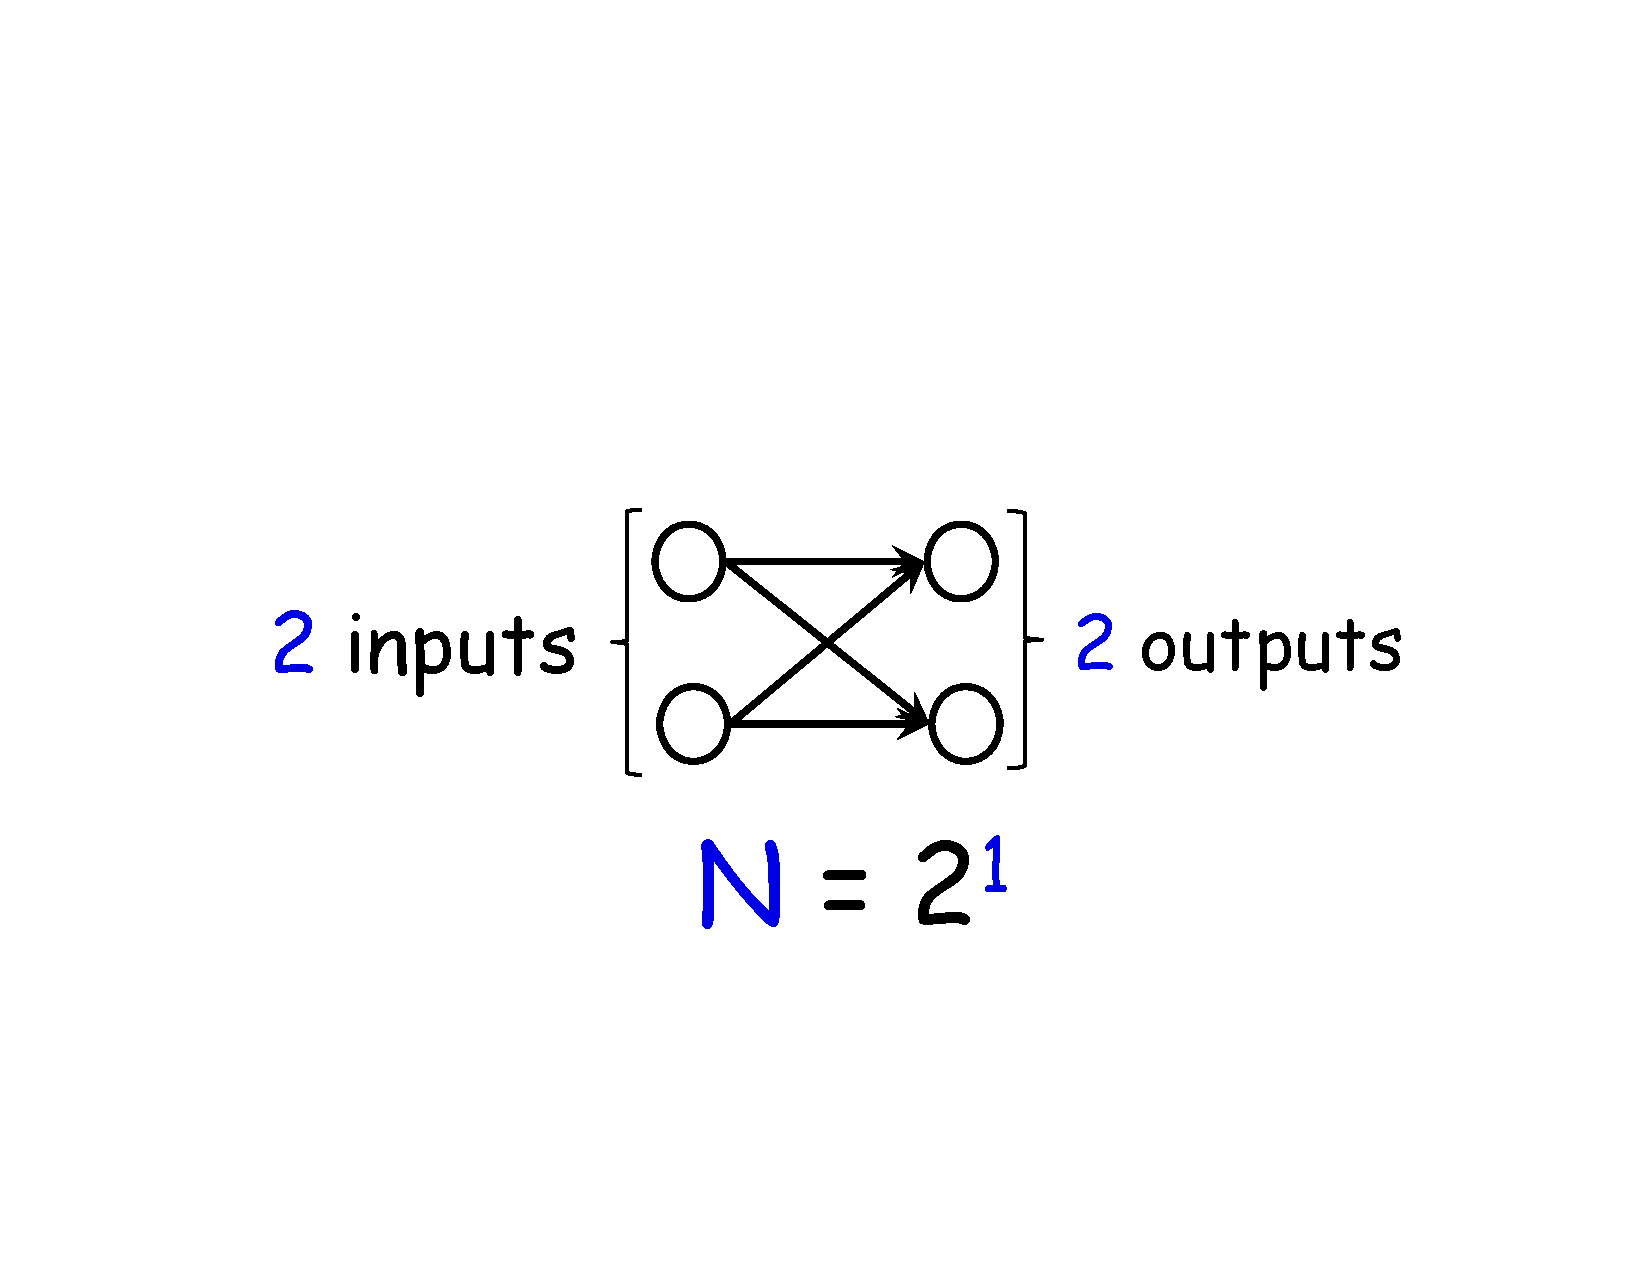
\includegraphics{figures/butterfly-base}
\end{center}
\caption{$F_1$, the Butterfly Net switches with $N=2^1$.}
\label{fig:butterfly-base}
\end{figure}

\begin{staffnotes}

The butterfly of size $2N$ consists of two butterflies of size $N$, which
are shown in dashed boxes below, and one additional level of switches.
Each switch in the new level has directed edges to a pair of
corresponding switches in the smaller butterflies; one example is
dashed in the figure.

\mfigure{!}{3in}{figures/butterfly3}

Despite the relatively complicated structure of the butterfly, there
is a simple way to route packets.  In particular, suppose that we want
to send a packet from input $x_1 x_2 \dots x_{\log N}$ to output $y_1
y_2 \dots y_{\log N}$.  (Here we are specifying the input and output
numbers in binary.)  Roughly, the plan is to ``correct'' the first bit
by level 1, correct the second bit by level 2, and so forth.  Thus,
the sequence of switches visited by the packet is:
%
\begin{align*}
(x_1, x_2, x_3, \dots, x_{\log N}, 0)
    & \to (y_1, x_2, x_3, \dots, x_{\log N}, 1) \\
    & \to (y_1, y_2, x_3, \dots, x_{\log N}, 2) \\
    & \to (y_1, y_2, y_3, \dots, x_{\log N}, 3) \\
    & \to \qquad \dots \\
    & \to (y_1, y_2, y_3, \dots, y_{\log N}, \log N) \\
\end{align*}
%
In fact, this is the \textit{only} path from the input to the output!

\end{staffnotes}

In the constructor step, we construct $F_{n+1}$ with $2^{n+1}$ inputs and
outputs out of two $F_n$ nets connected to a new set of $2^{n+1}$ input
switches, as shown in as in Figure~\ref{fig:butterfly-recursive}.  That
is, the $i$th and $2^n+i$th new input switches are each connected to the
same two switches, namely, to the $i$th input switches of each of two
$F_n$ components for $i=1,\dots,2^n$.  The output switches of $F_{n+1}$
are simply the output switches of each of the $F_n$ copies.

\begin{figure}[h]
\begin{center}
\mfigure{!}{3in}{figures/butterfly-recursive}
%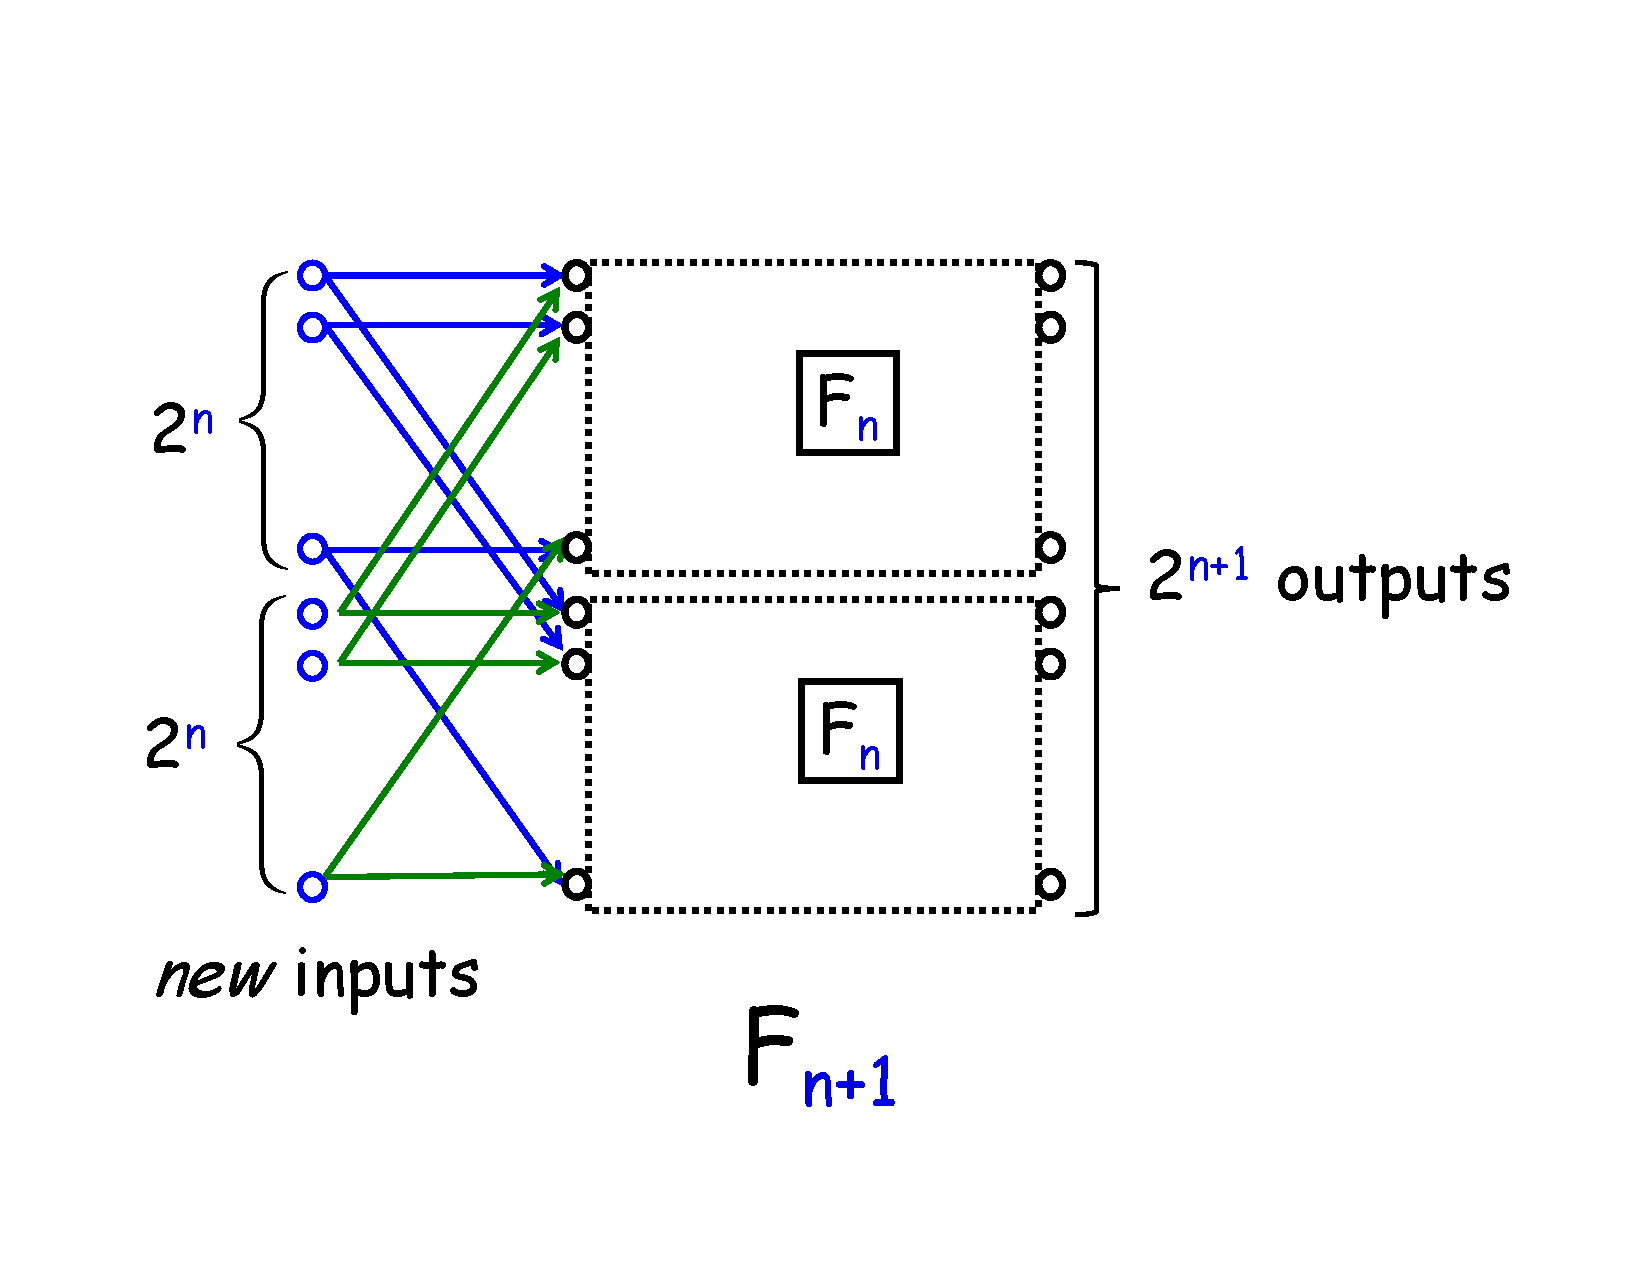
\includegraphics{figures/butterfly-recursive}
\end{center}
\caption{$F_{n+1}$, the Butterfly Net switches with $2^{n+1}$ inputs
and outputs.}
\label{fig:butterfly-recursive}
\end{figure}

So $F_{n+1}$ is laid out in columns of height $2^{n+1}$ by adding one more
column of switches to the columns in $F_n$.  Since the construction starts
with two columns when $n=1$, the $F_{n+1}$ switches are arrayed in $n+1$
columns.  The total number of switches is the height of the columns times
the number of columns, namely, $2^{n+1}(n+1)$.  Remembering that $n=\log
N$, we conclude that the Butterfly Net with $N$ inputs has $N(\log N +1)$
switches.

Since every path in $F_{n+1}$ from an input switch to an output is the
same length, namely, $n+1$, the diameter of the Butterfly net with
$2^{n+1}$ inputs is this length plus two because of the two edges
connecting to the terminals (square boxes) ---one edge from input
terminal to input switch (circle) and one from output switch to output
terminal.

There is an easy recursive procedure to route a packet through the
Butterfly Net.  In the base case, there is obviously only one way to route
a packet from one of the two inputs to one of the two outputs.  Now
suppose we want to route a packet from an input switch to an output switch
in $F_{n+1}$.  If the output switch is in the ``top'' copy of $F_n$, then
the first step in the route must be from the input switch to the unique
switch it is connected to in the top copy; the rest of the route is
determined by recursively routing the rest of the way in the top copy of
$F_n$.  Likewise, if the output switch is in the ``bottom'' copy of $F_n$,
then the first step in the route must be to the switch in the bottom copy,
and the rest of the route is determined by recursively routing in the
bottom copy of $F_n$.  In fact, this argument shows that the routing is
\emph{unique}: there is exactly one path in the Butterfly Net from each
input to each output, which implies that the network latency when
minimizing congestion is the same as the diameter.

The congestion of the butterfly network is about $\sqrt{N}$, more
precisely, the congestion is $\sqrt{N}$ if $N$ is an even power of 2 and
$\sqrt{N/2}$ if $N$ is an odd power of 2.  A simple proof of this appears
in Problem\ref{PS_butterfly_congestion}.

Let's add the butterfly data to our comparison table:
%
\[
\begin{array}{r|c|c|c|c}
\textbf{network} &
\textbf{diameter} &
\textbf{switch size} &
\textbf{\# switches} &
\textbf{congestion} \\ \hline
\text{complete binary tree} & 2 \log N + 2 & 3 \times 3 & 2N - 1 & N \\
\text{2-D array} & 2 N & 2 \times 2 & N^2 & 2 \\
\text{butterfly} & \log N + 2 & 2 \times 2 & N (\log(N) + 1) & \sqrt{N} \text{ or } \sqrt{N/2}
\end{array}
\]
%
The butterfly has lower congestion than the complete binary tree.  And
it uses fewer switches and has lower diameter than the array.
However, the butterfly does not capture the best qualities of each
network, but rather is a compromise somewhere between the two.  So our
quest for the Holy Grail of routing networks goes on.

\section{Bene\u{s} Network}

In the 1960's, a researcher at Bell Labs named Bene\u{s} had a
remarkable idea.  He obtained a marvelous communication network with
congestion 1 by placing \textit{two} butterflies back-to-back.  This
amounts to recursively growing \term{Bene\u{s} nets} by adding both inputs
and outputs at each stage.  Now we recursively define $B_n$ to be the
switches and connections (without the terminals) of the Bene\u{s} net
with $N \eqdef 2^n$ input and output switches.

The base case, $B_1$, with 2 input switches and 2 output switches is
exactly the same as $F_1$ in Figure~\ref{fig:butterfly-base}.

In the constructor step, we construct $B_{n+1}$ out of two $B_n$ nets
connected to a new set of $2^{n+1}$ input switches \emph{and also} a
new set of $2^{n+1}$ output switches.  This is illustrated in
Figure~\ref{fig:benes-recursive}.

Namely, the $i$th and $2^n+i$th new input switches are each connected to
the same two switches, namely, to the $i$th input switches of each of two
$B_n$ components for $i=1,\dots,2^n$, exactly as in the Butterfly net.  In
addition, the $i$th and $2^n+i$th new \emph{output} switches are connected
to the same two switches, namely, to the $i$th output switches of each of
two $B_n$ components.

\begin{figure}[h]
\begin{center}
\mfigure{!}{4in}{figures/benes-recursive}
%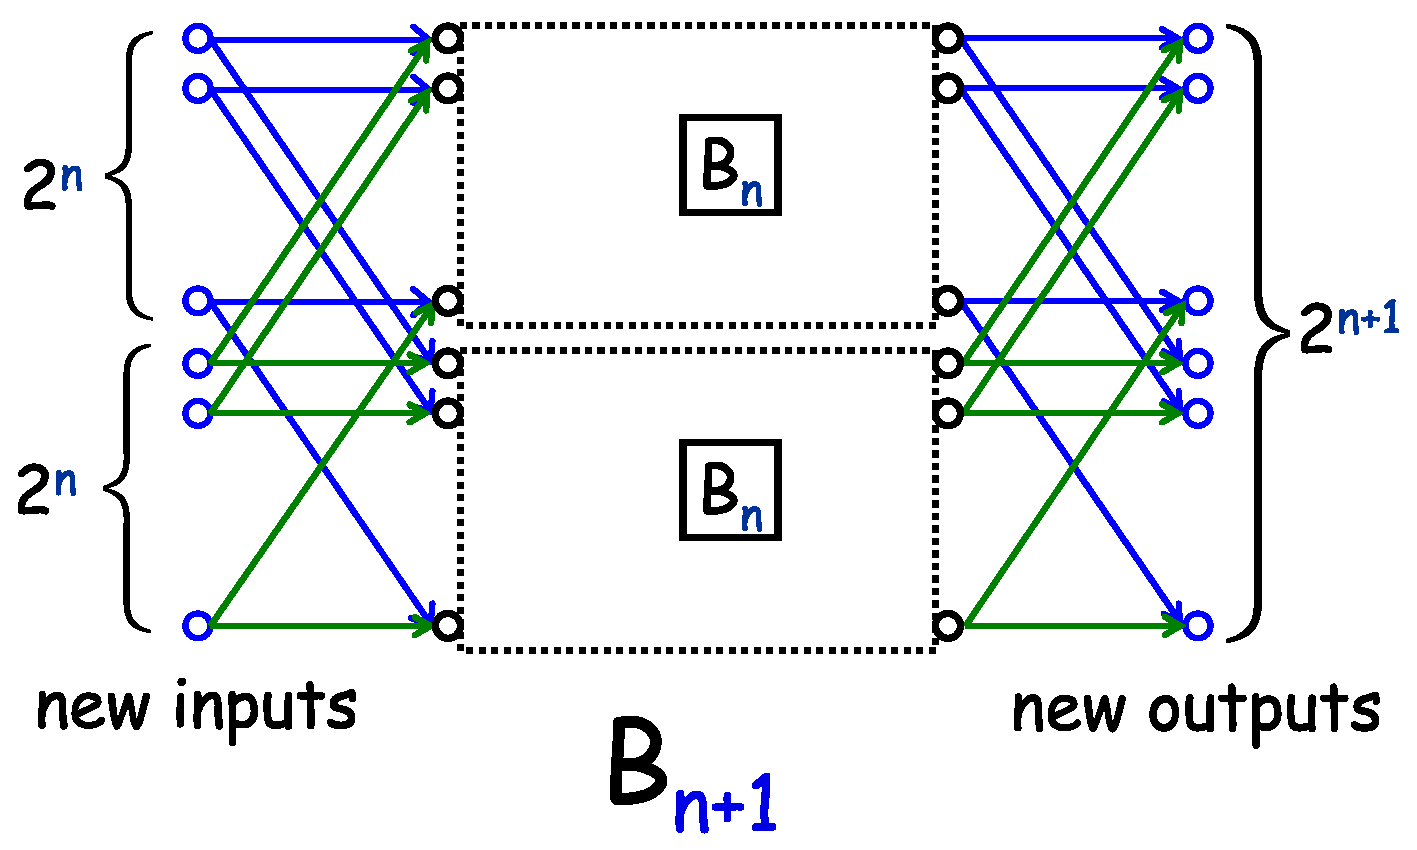
\includegraphics{figures/benes-recursive}
\end{center}
\caption{$B_{n+1}$, the Bene\u{s} Net switches with $2^{n+1}$ inputs
and outputs.}
\label{fig:benes-recursive}
\end{figure}

Now $B_{n+1}$ is laid out in columns of height $2^{n+1}$ by adding two
more columns of switches to the columns in $B_n$.  So the $B_{n+1}$
switches are arrayed in $2(n+1)$ columns.  The total number of
switches is the number of columns times the height of the columns,
namely, $2(n+1)2^{n+1}$.

All paths in $B_{n+1}$ from an input switch to an output are the same
length, namely, $2(n+1)-1$, and the diameter of the Bene\u{s} net with
$2^{n+1}$ inputs is this length plus two because of the two edges
connecting to the terminals.

\begin{staffnotes}

\mfigure{5in}{!}{figures/benes}

% This should make the construction of the 2-colorable graph in the
% congestion proof just a little more apparent.

This network now has levels labeled $0,\dots ,2 \log N + 1$. For $1 \leq k
\leq \log N$, the connections from level $k-1$ to level $k$ are just as in
the Butterfly network, the connections based on bit $k$. The conections
from level $2 \log N - k + 1$ to level $2 \log N - k + 2$ are also the
ones based on bit $k$.  (Informally, to make the connections from level
$0$ to level $2 \log N +1$ one level at a time, use the connections based
on bits $1,2,3,\dots, \log N - 1, \log N, \log N - 1, \log N - 2, \dots,
3,2,1$ in that order.)

\end{staffnotes}

So Bene\u{s} has doubled the number of switches and the diameter, of
course, but completely eliminates congestion problems!  The proof of
this fact relies on a clever induction argument that we'll come to in
a moment.  Let's first see how the Bene\u{s} network stacks up:
%
\[
\begin{array}{r|c|c|c|c}
\textbf{network} &
\textbf{diameter} &
\textbf{switch size} &
\textbf{\# switches} &
\textbf{congestion} \\ \hline
\text{complete binary tree} & 2 \log N + 2 & 3 \times 3 & 2N - 1 & N \\
\text{2-D array} & 2 N & 2 \times 2 & N^2 & 2 \\
\text{butterfly} & \log N + 2 & 2 \times 2 & N (\log(N) + 1) & \sqrt{N} \text{ or } \sqrt{N/2} \\
\text{Bene\u{s}} & 2 \log N + 1 & 2 \times 2 &  2 N \log N & 1
\end{array}
\]
%
The Bene\u{s} network has small size and diameter, and completely
eliminates congestion.  The Holy Grail of routing networks is in hand!

\begin{theorem}
The congestion of the $N$-input Bene\u{s} network is 1.

\iffalse , where $N = 2^a$ for some $a \geq 1$\fi

\end{theorem}

\begin{proof}
By induction on $n$ where $N=2^n$.  So the induction hypothesis is

\[
P(n) \eqdef  \text{the congestion of $B_n$ is 1}.
\]

\textbf{Base case} ($n=1$): $B_1 =F_1$ and the unique routings in $F_1$
have congestion 1.

\textbf{Inductive step}: We assume that the congestion of an $N=2^n$-input
Bene\u{s} network is 1 and prove that the congestion of a $2N$-input
Bene\u{s} network is also 1.

\textbf{Digression. }  Time out!  Let's work through an example,
develop some intuition, and then complete the proof.  In the Bene\u{s}
network shown below with $N=8$ inputs and outputs, the two
4-input/output subnetworks are in dashed boxes.

\mfigure{!}{3in}{figures/benes-decomp}

By the inductive assumption, the subnetworks can each route an
arbitrary permutation with congestion 1.  So if we can guide packets
safely through just the first and last levels, then we can rely on
induction for the rest!  Let's see how this works in an example.
Consider the following permutation routing problem:
%
\begin{align*}
\pi(0) & = 1 & \pi(4) & = 3 \\
\pi(1) & = 5 & \pi(5) & = 6 \\
\pi(2) & = 4 & \pi(6) & = 0 \\
\pi(3) & = 7 & \pi(7) & = 2
\end{align*}

We can route each packet to its destination through either the upper
subnetwork or the lower subnetwork.  However, the choice for one
packet may constrain the choice for another.  For example, we can not
route both packet 0 \textit{and} packet 4 through the same network
since that would cause two packets to collide at a single switch,
resulting in congestion.  So one packet must go through the upper
network and the other through the lower network.  Similarly, packets 1
and 5, 2 and 6, and 3 and 7 must be routed through different networks.
Let's record these constraints in a graph.  The vertices are the 8
packets.  If two packets must pass through different networks, then
there is an edge between them.  Thus, our constraint graph looks like
this:

\mfigure{!}{1.5in}{figures/benes-const1}

Notice that at most one edge is incident to each vertex.

The output side of the network imposes some further constraints.  For
example, the packet destined for output 0 (which is packet 6) and the
packet destined for output 4 (which is packet 2) can not both pass
through the same network; that would require both packets to arrive
from the same switch.  Similarly, the packets destined for outputs 1
and 5, 2 and 6, and 3 and 7 must also pass through different switches.
We can record these additional constraints in our graph with gray
edges:

\mfigure{!}{1.5in}{figures/benes-const2}

Notice that at most one new edge is incident to each vertex.
The two lines drawn between vertices 2 and 6 reflect the two different
reasons why these packets must be routed through different networks.
However, we intend this to be a simple graph; the two lines still
signify a single edge.

Now here's the key insight: \textit{a 2-coloring of the graph
corresponds to a solution to the routing problem}.  In particular,
suppose that we could color each vertex either red or blue so that
adjacent vertices are colored differently.  Then all constraints are
satisfied if we send the red packets through the upper network and the
blue packets through the lower network.

The only remaining question is whether the constraint graph is
2-colorable, which is easy to verify:

\begin{lemma}\label{deg1-union}
  Prove that if the edges of a graph can be grouped into two sets such
  that every vertex has at most 1 edge from each set incident to it, then
  the graph is 2-colorable.
\end{lemma}

\begin{proof}
  Since the two sets of edges may overlap, let's call an edge that is in
  both sets a \emph{doubled edge}.

  We know from Theorem~\ref{odd-cycle} that all we have to do is show that
  every cycle has even length.  There are two cases:

  \textbf{Case 1}: [The cycle contains a doubled edge.]  No other edge can
  be incident to either of the endpoints of a doubled edge, since that
  endpoint would then be incident to two edges from the same set.  So a
  cycle traversing a doubled edge has nowhere to go but back and forth
  along the edge an even number of times.

  \textbf{Case 2}: [No edge on the cycle is doubled.]  Since each vertex
  is incident to at most one edge from each set, any path with no doubled
  edges must traverse successive edges that alternate from one set to the
  other.  In particular, a cycle must traverse a path of alternating edges
  that begins and ends with edges from different sets.  This means the
  cycle has to be of even length.
\end{proof}

For example, here is a 2-coloring of the constraint graph:

\mfigure{!}{1.75in}{figures/benes-const3}

The solution to this graph-coloring problem provides a start
on the packet routing problem:

We can complete the routing in the two smaller Bene\u{s} networks by
induction!  Back to the proof.  \textbf{End of Digression.}

Let $\pi$ be an arbitrary permutation of $\set{0, 1, \dots, N-1}$.  Let $G$
be the graph whose vertices are packet numbers $0, 1, \dots, N-1$ and whose edges
come from the union of these two sets:
\begin{align*}
E_1 \eqdef &  \set{\edge{u}{v} \suchthat \abs{u - v} = N/2},\ \text{and} \\
E_2 \eqdef &  \set{\edge{u}{w} \suchthat \abs{\pi(u) - \pi(w)} = N/2}.
\end{align*}
Now any vertex, $u$, is incident to at most two edges: a unique edge
$\edge{u}{v} \in E_1$ and a unique edge $\edge{u}{w} \in E_2$.  So
according to Lemma~\ref{deg1-union}, there is a 2-coloring for the
vertices of $G$.  Now route packets of one color through the upper
subnetwork and packets of the other color through the lower subnetwork.
Since for each edge in $E_1$, one vertex goes to the upper subnetwork and
the other to the lower subnetwork, there will not be any conflicts in the
first level.  Since for each edge in $E_2$, one vertex comes from the
upper subnetwork and the other from the lower subnetwork, there will not
be any conflicts in the last level.  We can complete the routing within
each subnetwork by the induction hypothesis $P(n)$.
\end{proof}

\begin{problems}
\examproblems
\pinput{MQ_basic_network_problem}

\classproblems
\pinput{CP_Benes_network}
\pinput{CP_binary-tree_network}
\pinput{CP_2_layer_array_network}
\pinput{CP_n-path_network}
\pinput{CP_Megumi_net}

\homeworkproblems
\pinput{PS_Reasoner_net}
\pinput{PS_butterfly_congestion}
\end{problems}

\iffalse
In class, you will work through an example in which you route packets
using this recursive idea!
\fi

\endinput

   %recursive; uses digraphs, simple graph coloring

\chapter{Graph Theory}\label{chap:graph_theory}

Informally, a graph is a bunch of dots and lines where the lines
connect some pairs of dots.  An example is shown in
Figure~\ref{fig:graph-example}.  The dots are called \emph{nodes} (or
\emph{vertices}) and the lines are called \emph{edges}.

\begin{figure}[h]

\redrawn

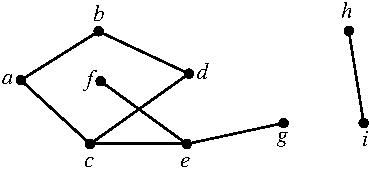
\includegraphics{graph-example}

\caption{An example of a graph with 9 nodes and 8 edges.}

\label{fig:graph-example}

\end{figure}

Graphs appear everywhere in computer science because they provide a handy
way to represent relationships between pairs of objects.  The objects
might be programs, people, cities, or web pages, and we connect two of
them with an edge if they are related in a certain way.  For example, an
edge between a pair of people might indicate that they like---or in
alternate scenarios that they don't like---each other.  An edge between a
pair of courses might indicate that they can't both be taken at the same
time.

In this chapter, we will focus on \emph{\idx{simple graphs}} where the
relationship denoted by an edge \emph{\idx{symmetric}}, meaning that the
relationship is mutual and edges don't have a direction.  Then in
Chapter~\ref{chap:digraphs}, we consider \emph{\idx{directed graphs}}
where an edge denotes a one-way relationship, for example, where one web
page points to the other.\footnote{Two Stanford students became
  multibillionaires because of their analyses of such web-page graphs.  So
  pay attention to graph theory, and who knows what might happen!}

\section{Definitions}\label{degreessec}

\subsection{Simple Graphs}

\begin{definition}\label{graphdef}
  A \term{simple graph}, $G$, consists of a nonempty set,~$\vertices{G}$,
  called the \term{vertices} of~$G$, and a set, $\edges{G}$, of
  two-element subsets of $\vertices{G}$.  The members of $E$ are called
  the \term{edges} of $G$.  Vertices are also called \term{nodes}; the
  terms ``vertex'' and ``node'' are used interchangeably.
\end{definition}
The vertices correspond to the dots in Figure~\ref{fig:graph-example},
and the edges correspond to the lines.  The graph, $G$, in
Figure~\ref{fig:graph-example}, is determined  mathematically by it
vertices and edges, namely,
\begin{align*}
\vertices{G} & =  \set{a, b, c, d, e, f, g, h, i} \\
\edges{G} & =  \set{\, \set{a, b}, \set{a, c}, \set{b, d}, \set{c, d},
              \set{c, e}, \set{e, f}, \set{e, g}, \set{h, i} \,}.
\end{align*}
%%  \begin{editingnotes}
%%  It will often be helpful to use the notation $\edge{a}{b}$ for the edge
%%  $\set{a,b}$.
%%  \end{editingnotes}
Note that $\edge{a}{b}$ and $\edge{b}{a}$ are different
descriptions of the same edge, since sets are unordered.  In this case,
the graph $G$ has 9~nodes and 8~edges.

\begin{definition}
Two vertices in a simple graph are said to be \term{adjacent} if they are
joined by an edge, and an edge is said to be \term{incident} to the
vertices it joins.  The number of edges incident to a vertex~$v$ is called
the \term{degree} of the vertex and is denoted by $\degr{v}$.
Equivalently, the degree of a vertex is equals the number of vertices
adjacent to it.
\end{definition}
For example, in the simple graph shown in
Figure~\ref{fig:graph-example}, vertex~$a$ is adjacent to vertex~$b$,
and $b$ is adjacent to~$d$.  The edge $\edge{a}{c}$ is incident to
vertices $a$ and~$c$.  Vertex~$h$ has degree~1, $d$ has degree~2, and
$\degr{e} = 3$.  It is possible for a vertex to have degree~0, in which
case it is not adjacent to any other vertices.  A simple graph, $G$, does
not need to have any edges at all, namely $\card{\edges{G}}$ could be
zero,\footnote{The \emph{cardinality}, $\card{E}$, of a set,~$E$, is the
number of elements in~$E$.} which would implies that the degree of every
vertex is also zero.  The graph may not have no vertices at all, namely,
$\card{\vertices{G}}$ is required to be at least one.

An arc going from a vertex back around to that same vertex, is called a
\term{self-loop}.  Self-loops aren't allowed in simple
graphs.\footnote{You might try to represent a self-loop going between a
  vertex, $v$, and itself as $\set{v, v}$, but this wouldn't be an edge
  because an edge is defined to be set of \emph{two} vertices.}  In more
general \term{multigraphs} there can be more than one edge between the
same two vertices, but this doesn't happen in simple graphs since all
edges between vertices $v$ and $w$ would equal the same set $\edge{v}{w}$.
Lastly, and most importantly, simple graphs do not contain \emph{directed
  edges}, that is, edges, $\diredge{v}{w}$ that go from a vertex $v$ to
vertex $w$, but not the other way from $w$ to $v$.

Sometimes graphs with no vertices, with self-loops, or with more than one
edge between the same two vertices are convenient to have, but we don't
need them, and it's simpler to stick to simple graphs \smiley.
\begin{editingnotes}
We will consider graphs with directed edges (called \emph{directed graphs} or
\emph{digraphs}) at length in Chapter~\ref{chap:digraphs}.
\end{editingnotes}
Since we'll only be considering simple graphs in this chapter, we'll just
call them ``graphs'' from now on.

\subsection{Some Common Graphs}

Some graphs come up so frequently that they have names.  The
\term{complete graph} on $n$ vertices, denoted $K_n$, has an edge
between every two vertices, for a total of $n(n-1)/2$ edges.  For
example, $K_5$ is shown in Figure~\ref{fig:K_5}.

\begin{figure}

\redrawn

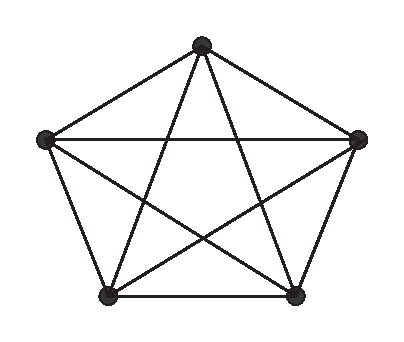
\includegraphics{complete-graph}

\caption{The complete graph on 5 nodes, $K_5$.}
\label{fig:K_5}
\end{figure}

The \term{empty graph} has no edges at all.  For example, the empty
graph with 5 nodes is shown in Figure~\ref{fig:graph_empty_5}.

\begin{figure}

\redrawn


\includegraphics{empty-graph}

\caption{The empty graph with 5 nodes.}
\label{fig:graph_empty_5}
\end{figure}

The $n$-node graph containing $n - 1$ edges in sequence is known as
the \emph{line graph}~$L_n$.  More formally, $L_n$ has
\begin{equation*}
    \vertices{L_n} = \set{ v_1, v_2, \dots, v_n }
\end{equation*}
and
\begin{equation*}
    \edges{L_n} = \set{\, \edge{v_1}{v_2}, \edge{v_2}{v_3}, \dots,
    \edge{v_{n-1}}{v_n} \, }
\end{equation*}
For example, $L_5$ is displayed in Figure~\ref{fig:graph_L_5}.

\begin{figure}

\redrawn

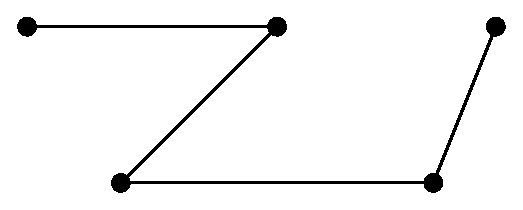
\includegraphics{path-graph}

\caption{The 5-node line graph~$L_5$.}

\label{fig:graph_L_5}

\end{figure}

If we add the edge $\edge{v_n}{v_1}$ to the line graph~$L_n$, we get a
graph called the \index{cycle}\term{length $n$ cycle}, \idx{$C_n$}.
Figure~\ref{fig:graph_C_5} shows a picture of $C_5$.

\begin{figure}

\redrawn

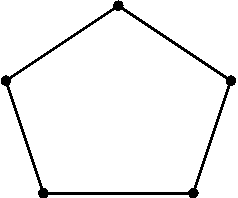
\includegraphics{cycle}

\caption{The 5-node cycle graph~$C_5$.}
\label{fig:graph_C_5}
\end{figure}

\subsection{Isomorphism}

Two graphs that look the same might actually be different in a formal
sense.  For example, the two graphs in Figure~\ref{fig:isomorphism}
are both cycles with 4~vertices, but one graph has vertex set
$\set{a, b, c, d}$ while the other has vertex set $\set{1, 2, 3, 4}$.
Strictly speaking, these graphs are different mathematical objects,
but this is a frustrating distinction since the graphs \emph{look the
same}!

\begin{figure}

\redrawn

\gnote{Geoff: Split this into two figures}

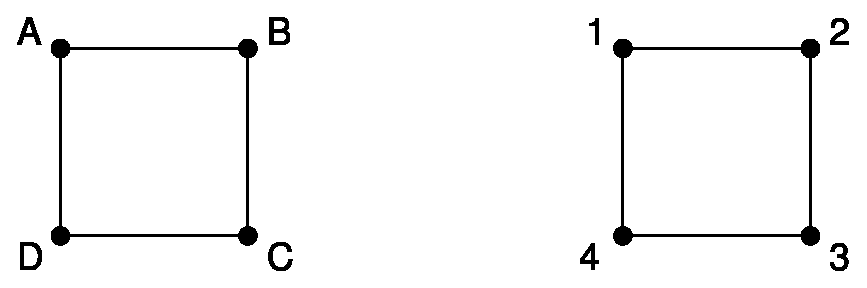
\includegraphics{isomorphism}

\caption{Two graphs that are isomorphic to~$C_4$.}
\label{fig:isomorphism}
\end{figure}

Fortunately, we can neatly capture the idea of ``looks the same''
through the notion of graph isomorphism.

\begin{editingnotes}
  def of bijection in footnote is garbled: every total function, f,
  associates a domain element, d, with a range element, f(d), uniquely
  determined by d.  What's meant of course is that f(d) uniquely
  determines d, but this is clear as written.  Better to pull the def
  of bijection out of the footnote and make it a careful def in
  the main text.  I'll refer back to this def later when I define a bij to
  be a total, inj \& surj function.---ARM, 7/4/10.
\end{editingnotes}

\begin{definition}\label{simple-isomorphism}
  Graph $G$ is \term{isomorphic} to graph $H$ iff there exists a
  \term{bijection}\footnote{A bijection $f: \vertices{G} \to \vertices{H}$
    is a function that associates every node in~$\vertices{G}$ with a
    unique node in~$\vertices{H}$ and vice-versa.  We will study
    bijections more deeply in Part~\ref{part:counting}.} $f:\vertices{G} \to \vertices{H}$
  such that for every pair of vertices $u, v \in \vertices{G}$:
\[
\edge{u}{v} \in \edges{G} \qiff \edge{f(u)}{f(v)} \in \edges{H}.
\]
The function $f$ is called an \term{isomorphism} between $G$ and $H$.
\end{definition}

In other words, two graphs are isomorphic if they are the same up to a
relabeling of their vertices.  For example, here is an isomorphism between
vertices in the two graphs shown in Figure~\ref{fig:isomorphism}:
\[
\begin{array}{lll}
a \text{ corresponds to } 1 & \hspace{0.5in} & b \text{ corresponds to } 2 \\
d \text{ corresponds to } 4 & & c \text{ corresponds to } 3.
\end{array}
\]
ou can check that there is an edge between two vertices in the graph
on the left if and only if there is an edge between the two
corresponding vertices in the graph on the right.

Two isomorphic graphs may be drawn very differently.  For example, we
have shown two different ways of drawing $C_5$ in
Figure~\ref{fig:isomorphism-c5}.

\begin{figure}

\redrawn

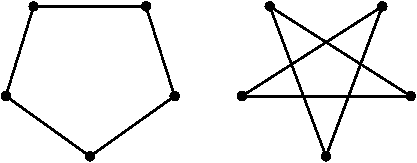
\includegraphics{isomorphism-c5}

\caption{Two ways of drawing $C_5$.}
\label{fig:isomorphism-c5}
\end{figure}

Isomorphism preserves the connection properties of a graph,
abstracting out what the vertices are called, what they are made out
of, or where they appear in a drawing of the graph.  More precisely, a
property of a graph is said to be \term{preserved under isomorphism}
if whenever $G$ has that property, every graph isomorphic to $G$ also
has that property.  For example, isomorphic graphs must have the same
number of vertices.  What's more, if $f$ is a graph isomorphism that
maps a vertex, $v$, of one graph to the vertex, $f(v)$, of an
isomorphic graph, then by definition of isomorphism, every vertex
adjacent to $v$ in the first graph will be mapped by $f$ to a vertex
adjacent to $f(v)$ in the isomorphic graph.  This means that $v$ and
$f(v)$ will have the same degree.  So if one graph has a vertex of
degree 4 and another does not, then they can't be isomorphic.  In
fact, they can't be isomorphic if the number of degree 4 vertices in
each of the graphs is not the same.

Looking for preserved properties can make it easy to determine that
two graphs are not isomorphic, or to actually find an isomorphism
between them if there is one.  In practice, it's frequently easy to
decide whether two graphs are isomorphic.  However, no one has yet
found a
\emph{general} procedure for determining whether two graphs are isomorphic
that is \emph{guaranteed} to run in polynomial
time\footnote{\emph{I.e.}, in an amount of time that is upper-bounded
  by $\card{V}^c$ where $c$ is a fixed number independent of~$\card{V}$.}
in~$\card{V}$.

Having such a procedure would be useful.  For example, it would make
it easy to search for a particular molecule in a database given the
molecular bonds.  On the other hand, knowing there is no such
efficient procedure would also be valuable: secure protocols for
encryption and remote authentication can be built on the hypothesis
that graph isomorphism is computationally exhausting.

\subsection{Subgraphs}

\begin{definition}\label{def:subgraph}
  A graph $G$ is said to be a \emph{subgraph} of a graph $H$ if
  $\vertices{G} \subseteq \vertices{H}$ and $\edges{G} \subseteq
  \edges{H}$.
\end{definition}

For example, the empty graph on $n$ nodes is a subgraph of~$L_n$,
the graph $L_n$ is a subgraph of~$C_n$, and $C_n$ is a subgraph of~$K_n$.
Also, the graph $G$ where
\begin{equation*}
   \vertices{G} = \set{ g, h, i } \quad \text{and}\quad  \edges{G} =
   \set{\, \set{h, i} \, }
\end{equation*}
is a subgraph of the graph in Figure~\ref{fig:graph-example}.  On the
other hand, any graph containing an edge~$\set{g, h}$ would not be a
subgraph of the graph in Figure~\ref{fig:graph-example} because the
graph in Figure~\ref{fig:graph-example} does not contain this edge.

Note that since a subgraph is itself a graph, the endpoints of any edge in
a subgraph must also be in the subgraph.  In other words if $G'$ is a
subgraph of some graph~$G$, and $\set{ v, w } \in \edges{G'}$, then it
must be the case that $v$ and $w$ are vertices of $G'$.

\subsection{Weighted Graphs}

Sometimes, we will use edges to denote a connection between a pair of
nodes where the connection has a \emph{capacity} or \emph{weight}.
For example, we might be interested in the capacity of an Internet
fiber between a pair of computers, the resistance of a wire between a
pair of terminals, the tension of a spring connecting a pair of
devices in a dynamical system, the tension of a bond between a pair of
atoms in a molecule, or the distance of a highway between a pair of
cities.

In such cases, it is useful to represent the system with an
\emph{edge-weighted} graph (aka a \emph{weighted graph}).  A weighted
graph is the same as a simple graph except that we associate a real
number (\ie the weight) with each edge in the graph.  Mathematically
speaking, a weighted graph consists of a graph $G$ and a
weight function $w: \edges{G} \to \reals$.  For example,
Figure~\ref{fig:weighted_graph} shows a weighted graph where the
weight of edge $\edge{a}{b}$ is~5.

\begin{figure}

\redrawn

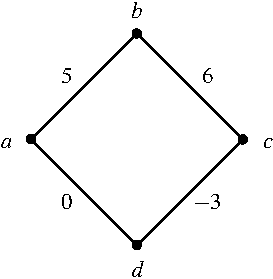
\includegraphics{Fig_5D}

\caption{A 4-node weighted graph where the edge~$\edge{a}{b}$ has
  weight~5.}
\label{fig:weighted_graph}
\end{figure}

\subsection{Adjacency Matrices}

There are many ways to represent a graph.  We have already seen two ways:
you can draw it, as in Figure~\ref{fig:weighted_graph} for example, or you
can represent it with sets of vertices and edges.  Another common
representation is with an adjacency matrix.

\begin{definition}\label{def:adjacency_matrix}

Given an $n$-node graph $G$ where $\vertices{G} = set{ v_1, v_2, \dots,
v_n }$, the \term{adjacency matrix} for~$G$ is the $n \by n$ matrix
$A_G = \set{ a_{ij} }$ where
\begin{equation*}
    a_{ij} = \begin{cases}
                1 & \text{if $\set{ v_i, v_j } \in \edges{G}$} \\
                0 & \text{otherwise.}
              \end{cases}
\end{equation*}
If $G$ is a weighted graph with edge weights given by $w: \edges{G} \to
\reals$, then the adjacency matrix for~$G$ is $A_G = \{ a_{ij} \}$
where
\begin{equation*}
    a_{ij} = \begin{cases}
                w(\{ v_i, v_j \}) & \text{if $\{ v_i, v_j \} \in \edges{G}$} \\
                0                 & \text{otherwise.}
              \end{cases}
\end{equation*}
\end{definition}

For example, Figure~\ref{fig:adjacency_matrix} displays the adjacency
matrices for the graphs shown in Figures~\ref{fig:isomorphism}(a)
and~\ref{fig:weighted_graph} where $v_1 = a$, $v_2 = b$, $v_3 = c$,
and $v_4 = d$.

\begin{figure}
\normalbaselines
\subfloat[]{%
    $
       \begin{pmatrix}
           0 & 1 & 0 & 1 \\
           1 & 0 & 1 & 0 \\
           0 & 1 & 0 & 1 \\
           1 & 0 & 1 & 0
       \end{pmatrix}
   $
}
\qquad
\subfloat[]{%
   $
       \begin{pmatrix}
           0 & 5 & 0 & 0 \\
           5 & 0 & 6 & 0 \\
           0 & 6 & 0 & -3 \\
           0 & 0 & -3 & 0
       \end{pmatrix}
   $
}

\caption{Examples of adjacency matrices.  (a)~shows the adjacency
  matrix for the graph in Figure~\ref{fig:isomorphism}(a) and
  (b)~shows the adjacency matrix for the weighted graph in
  Figure~\ref{fig:weighted_graph}.  In each case, we  set $v_1
  = a$, $v_2 = b$, $v_3 = c$, and $v_4 = d$ to construct the matrix.}
\label{fig:adjacency_matrix}
\end{figure}

%% Simple Graphs Problems %%%%%%%%%%%%%%%%%%%%%%%%%%%%%%%%%%%%%%%%%%%%%%%%%%%%%
\begin{problems}
\classproblems
\pinput{CP_Handshaking_Lemma}
\pinput{CP_isomorphic_graphs}
% S09.cp6m.1
% S09.cp6m.3
% S09.cp6m.4

\homeworkproblems
\pinput{PS_choose_isomorphic_graphs}
\pinput{PS_neighbors_under_isomorphisms}
\pinput{PS_graph_two_ends}

\examproblems
\pinput{MQ_list_isomorphisms}
\end{problems}


\section{Matching Problems}\label{sexam}

For our first serious applications of graph theory we'll look at scenarios
where the nodes in a graph represent people and the edges represent a
relationship between pairs of people such as ``likes,'' ``marries,'' ``has
a common interest,'' and so on.  Now, you have good reason to wonder what
marriages have to do with computer science.  We'll explain how the
techniques we describe to find marriage compatible men and women are
also widely applied in practice to scenarios where applicants must be to
matched to jobs, packets matched to paths in a network, or Internet
traffic matched to web servers.  

To begin, we will show how graph theory can be used to debunk an urban
legend about sexual practices in America.  Yes, you read correctly.  So,
fasten your seat belt---who knew that math might actually be interesting!

\subsection{Sex in America}

On average, who has more opposite-gender partners: men or women?

Sexual demographics have been the subject of many studies.  In one of the
largest, researchers from the University of Chicago interviewed a random
sample of 2500 Americans over several years to try to get an answer to this
question.  Their study, published in 1994, and entitled \emph{The Social
  Organization of Sexuality} found that, on average, men have 74\% more
opposite-gender partners than women.

Other studies have found that the disparity is even larger.  In
particular, ABC News claimed that the average man has 20 partners over his
lifetime, and the average woman has 6, for a percentage disparity of
233\%.  The ABC News study, aired on Primetime Live in 2004, purported to
be one of the most scientific ever done, with only a 2.5\% margin of
error.  It was called ``American Sex Survey: A peek between the sheets.''
The promotion for the study is even better:
\begin{quote}
A ground breaking ABC News ``Primetime Live'' survey finds a range of
eye-popping sexual activities, fantasies and attitudes in this country,
confirming some conventional wisdom, exploding some myths---and venturing
where few scientific surveys have gone before.
\end{quote}
Probably that last part about going where few scientific surveys have gone
before is pretty accurate!

Yet again, in August, 2007, the N.Y. Times reported
%% \href{The-Myth-the-Math-the-Sex.pdf}{reported}
%% \iffalse
%% \href{http://www.nytimes.com/2007/08/12/weekinreview/12kolata.html?_r=1&n=Top/Reference/Times%20Topics/People/K/Kolata,%20Gina&oref=slogin}{reported}
%% \fi
on a study by the National Center for Health Statistics of the
U.S. Government showing that men had seven partners while women had
four.

Anyway, whose numbers do you think are more accurate, the University
of Chicago, ABC News, or the National Center for Health
Statistics?---don't answer; this is a setup question like ``When did
you stop beating your wife?''  Using a little graph theory, we will
now explain why none of these findings can be anywhere near the truth.

Let's model the question of heterosexual partners in graph theoretic
terms.  To do this, we'll let $G$ be the graph whose vertices, $V$,
are all the people in America.  Then we split $V$ into two separate
subsets: $M$, which contains all the males, and $F$, which contains
all the females.\footnote{For simplicity, we'll ignore the possibility
  of someone being both, or neither, a man and a woman.}  We'll put an
edge between a male and a female iff they have been sexual partners.
A possible subgraph of this graph is illustrated in
Figure~\ref{fig:partners} with males on the left and females on the
right.

\begin{figure}[htbp]

\redrawn

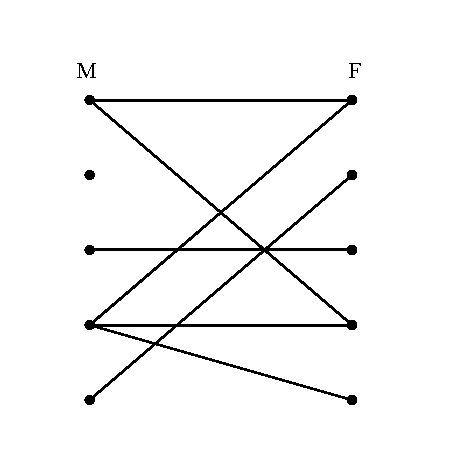
\includegraphics{sex-edges}

\caption{A possible subgraph of the sex partners graph.}
\label{fig:partners}
\end{figure}

Actually, $G$ is a pretty hard graph to figure out, let alone draw.
The graph is \emph{enormous}: the US population is about 300 million,
so $\card{V} \approx 300M$.  In the United States, approximately
50.8\% of the populatin is female and 49.2\% is male, and so $\card{M}
\approx 147.6M$, and $\card{F} \approx 152.4M$.  And we don't even
have trustworthy estimates of how many edges there are, let alone
exactly which couples are adjacent.  But it turns out that we don't
need to know any of this to debunk the sex surveys---we just need to
figure out the relationship between the average number of partners per
male and partners per female.  To do this, we note that every edge is
incident to exactly one $M$ vertex and one $F$ vertex (remember, we're
only considering male-female relationships); so the sum of the degrees
of the $M$ vertices equals the number of edges, and the sum of the
degrees of the $F$ vertices equals the number of edges.  So these sums
are equal:
%
\[
\sum_{x \in M} \degr{x} = \sum_{y \in F} \degr{y}.
\]
%
If we divide both sides of this equation by the product of the sizes
of the two sets, $\card{M} \cdot \card{F}$, we obtain
%
\begin{equation}\label{eq:average-degree}
\left(\frac{\sum_{x \in M} \degr{x}}{\card{M}}\right) \cdot \frac{1}{\card{F}} =
\left(\frac{\sum_{y \in F} \degr{y}}{\card{F}}\right) \cdot \frac{1}{\card{M}}
\end{equation}
Notice that
\begin{equation*}
    \frac{\sum_{x \in M} \degr{x}}{\card{M}}
\end{equation*}
is simply the average degree of a node in~$M$.  This is the average
number of opposite-gender partners for a male in America.  Similarly,
\begin{equation*}
    \frac{\sum_{x \in F} \degr{x}}{\card{F}}
\end{equation*}
is the average degree of a node in~$F$, which is the average number of
opposite-gender partners for a female in America.  Hence,
Equation~\ref{eq:average-degree} implies that on average, an American
male has $\card{F}/\card{M}$ times as many opposite-gender partners as the
average American female.

From the Census Bureau reports, we know that there are slightly more
females than males in America; in particular $\card{F} / \card{M}$ is
about~1.035.  So we know that on average, males have 3.5\% more
opposite-gender partners than females.  Of course, this statistic
really says nothing about
any sex's promiscuity or selectivity.  Remarkably, promiscuity is
completely irrelevant in this analysis.  That is because the ratio of
the average number of partners is completely determined by the
relative number of males and females.  Collectively, males and
females have the same number of opposite gender partners, since it
takes one of each set for every partnership, but there are fewer
males, so they have a higher ratio.  This means that the University of
Chicago, ABC, and the Federal Government studies are way off.  After a
huge effort, they gave a totally wrong answer.

There's no definite explanation for why such surveys are consistently
wrong.  One hypothesis is that males exaggerate their number of
partners---or maybe females downplay theirs---but these explanations
are speculative.  Interestingly, the principal author of the National
Center for Health Statistics study reported that she knew the results
had to be wrong, but that was the data collected, and her job was to
report it.

The same underlying issue has led to serious misinterpretations of
other survey data.  For example, a few years ago, the Boston Globe ran
a story on a survey of the study habits of students on Boston area
campuses.  Their survey showed that on average, minority students
tended to study with non-minority students more than the other way
around.  They went on at great length to explain why this ``remarkable
phenomenon'' might be true.  But it's not remarkable at all---using
our graph theory formulation, we can see that all it says is that
there are fewer minority students than non-minority students, which
is, of course what ``minority'' means.

\subsubsection{The Handshaking Lemma}

The previous argument hinged on the connection between a sum of
degrees and the number edges.  There is a simple connection between
these quantities in any graph:
\begin{lemma}[The Handshaking Lemma]\label{sumedges}
The sum of the degrees of the vertices in a graph equals twice the
number of edges.
\end{lemma}

\begin{proof}
Every edge contributes two to the sum of the degrees, one for each of
its endpoints.
\end{proof}

Lemma~\ref{sumedges} is called the \term{Handshake Lemma} because if
we total up the number of people each person at a party shakes hands
with, the total will be twice the number of handshakes that occurred.

\subsection{Bipartite Matchings}\label{bipartitesec}
\begin{editingnotes}
\subsubsection*{Bipartite Graphs}\label{bipartitesubsec}
\end{editingnotes}

There were two kinds of vertices in the ``Sex in America''
graph---males and females, and edges only went between the two kinds.
Graphs like this come up so frequently that they have earned a special
name---they are called \emph{bipartite graphs}.

\begin{definition}
A \term{bipartite graph} is a graph together with a partition of its
vertices into two sets, $L$ and $R$, such that every edge is incident to a
vertex in $L$ and to a vertex in $R$.
\end{definition}

So every bipartite graph looks something like the graph in
Figure~\ref{fig:partners}.

\subsubsection{The Bipartite Matching Problem}

The bipartite matching problem is related to the sex-in-America
problem that we just studied; only now the goal is to get everyone
happily married.  As you might imagine, this is not possible for a
variety of reasons, not the least of which is the fact that there are
more women in America than men.  So, it is simply not possible to
marry every woman to a man so that every man is married only once.

But what about getting a mate for every man so that every woman is
married only once?  Is it possible to do this so that each man is
paired with a woman that he likes? The answer, of course, depends on
the bipartite graph that represents who likes who, but the good news
is that it is possible to find natural properties of the who-likes-who
graph that completely determine the answer to this question.

In general, suppose that we have a set of men and an equal-sized or
larger set of women, and there is a graph with an edge between a man
and a woman if the man likes the woman.  (Note that in this scenario,
the ``likes'' relationship need not be symmetric, since for the time
being, we will only worry about finding a mate for each man that he
likes.\footnote{By the way, we do not mean to imply that marriage
  should or should not be of a heterosexual nature.  Nor do we mean to
  imply that men should get their choice instead of women.  It's just
  that with bipartite graphs, the edges only connected male nodes to
  female nodes and there are fewer men in America.  So please don't
  take offense.}  (Later, we will consider the ``likes'' relationship
from the female perspective as well.)  For example, we might obtain
the graph in Figure~\ref{fig:5J}.

\begin{figure}

\redrawn

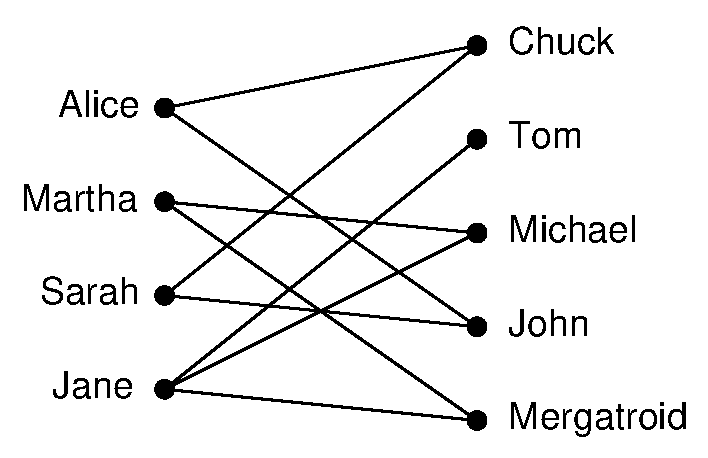
\includegraphics{hall-graph}

\caption{A graph where an edge between a man and woman denotes that
  the man likes the woman.}

\label{fig:5J}

\end{figure}

In this problem, a \term{matching} will mean a way of assigning every
man to a woman so that different men are assigned to different women,
and a man is always assigned to a woman that he likes.  For example,
one possible matching for the men is shown in Figure~\ref{fig:5K}.

\begin{figure}

\redrawn

\gnote[Geoff: Make heavy lines heavier.  Tom: We couldn't
  figure out what was intended here: these edges are inconsistent with
the text.]

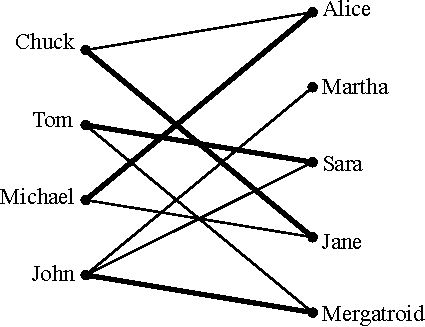
\includegraphics{hall-graph-matched}

\caption{One possible matching for the men is shown with bold edges.
  For example, John is matched with Jane.}

\label{fig:5K}

\end{figure}

\subsubsection{The Matching Condition}

A famous result known as \idx{Hall's Matching Theorem} gives necessary
and sufficient conditions for the existence of a matching in a
bipartite graph.  It turns out to be a remarkably useful mathematical
tool.

We'll state and prove Hall's Theorem using man-likes-woman
terminology.  Define \emph{the set of women liked by a given set of
  men} to consist of all women liked by at least one of those men.
For example, the set of women liked by Tom and John in
Figure~\ref{fig:5J} consists of Martha, Sarah, and Mergatroid.  For us
to have any chance at all of matching up the men, the following
\term{matching condition} must hold:

\medskip

\noindent\text{\emph{The Matching Condition}: every subset of men
  likes at least as large a set of women.}

\medskip

For example, we can not find a matching if some set of 4~men like only
3~women.  Hall's Theorem says that this necessary condition is
actually sufficient; if the matching condition holds, then a matching
exists.

\begin{theorem}\label{thm:matching}
A matching for a set of men~$M$ with a set of women~$W$ can be found
if and only if the matching condition holds.
\end{theorem}

\begin{proof}
First, let's suppose that a matching exists and show that the matching
condition holds.  Consider an arbitrary subset of men.  Each man likes
at least the woman he is matched with.  Therefore, every subset of men
likes at least as large a set of women.  Thus, the matching condition
holds.

Next, let's suppose that the matching condition holds and show that a
matching exists.  We use strong induction on $\card{M}$, the number of
men, on the predicate:
\begin{align*}
    P(m) ::={} & \text{for any set of $m$ men~$M$, if the matching
      condition holds} \\
             & \text{for~$M$, then there is a matching for~$M$.}
\end{align*}

\inductioncase{Base Case} ($\card{M}=1$): If $\card{M} = 1$, then the
matching condition implies that the lone man likes at least one woman,
and so a matching exists.

\inductioncase{Inductive Step:} We need to show that $P(m) \QIMPLIES
P(m + 1)$.  Suppose that $\card{M} = m + 1 \ge 2$.
\begin{description}

\item[Case 1:] Every proper subset\footnote{Recall that a subset $A$
  of~$B$ is \emph{proper} if $A \ne B$.} of men likes a \emph{strictly
  larger} set of women.  In this case, we have some latitude: we pair
  an arbitrary man with a woman he likes and send them both away.  The
  matching condition still holds for the remaining men and women since
  we have removed only one woman, so we can match the rest of the
  men by induction.

\item[Case 2:] Some proper subset of men $X \subset M$ likes an
  \emph{equal-size} set of women $Y \subset W$.  We match the men in
  $X$ with the women in $Y$ by induction and send them all away.  We
  can also match the rest of the men by induction if we show that the
  matching condition holds for the remaining men and women.  To check
  the matching condition for the remaining people, consider an
  arbitrary subset of the remaining men $X' \subseteq (M - X)$, and
  let $Y'$ be the set of remaining women that they like.  We must show
  that $\card{X'} \leq \card{Y'}$.  Originally, the combined set of
  men $X \cup X'$ liked the set of women $Y \cup Y'$.  So, by the
  matching condition, we know:
%
  \begin{equation*}
  \card{X \cup X'}  \leq  \card{Y \cup Y'}
  \end{equation*}
%
  We sent away $\card{X}$ men from the set on the left (leaving $X'$)
  and sent away an equal number of women from the set on the right
  (leaving $Y'$).  Therefore, it must be that $\card{X'} \leq
  \card{Y'}$ as claimed.
\end{description}

So in both cases, there is a matching for the men, which completes the
proof of the Inductive step.  The theorem follows by induction.
\end{proof}

The proof of Theorem~\ref{thm:matching} gives an algorithm for finding
a matching in a bipartite graph, albeit not a very efficient one.
However, efficient algorithms for finding a matching in a bipartite
graph do exist.  Thus, if a problem can be reduced to finding a
matching, the problem is essentially solved from a computational
perspective.

\subsubsection{A Formal Statement}

Let's restate Theorem~\ref{thm:matching} in abstract terms so that
you'll not always be condemned to saying, ``Now this group of men
likes at least as many women\dots''

\begin{definition}\label{def:5K}

A \term{matching} in a graph, $G$, is a set of edges such that no two
edges in the set share a vertex.  A matching is said to \emph{cover} a
set, $L$, of vertices iff each vertex in $L$ has an edge of the
matching incident to it.  A matching is said to be \emph{perfect} if
every node in the graph is incident to an edge in the matching.  In
any graph, the set $N(S)$, of \term{neighbors} of some set, $S$, of
vertices is the set of all vertices adjacent to some vertex in $S$.
That is,
\[
N(S) \eqdef \set{\,r \suchthat \edge{s}{r}\text{ is an edge for some }s \in S\,}.
\]
$S$ is called a \term{bottleneck} if
\[
\card{S} > \card{N(S)}.
\]
\end{definition}

\begin{theorem}[\idx{Hall's Theorem}]\label{thm:halls}
  Let $G$ be a bipartite graph with vertex partition $L,R$.  There is matching in $G$
  that covers $L$ iff no subset of $L$ is a bottleneck.
\end{theorem}

\subsubsection{An Easy Matching Condition}

The bipartite matching condition requires that \emph{every} subset of
men has a certain property.  In general, verifying that every subset
has some property, even if it's easy to check any particular subset
for the property, quickly becomes overwhelming because the number of
subsets of even relatively small sets is enormous---over a billion
subsets for a set of size 30.  However, there is a simple property of
vertex degrees in a bipartite graph that guarantees the existence of a
matching.  Namely, call a bipartite graph \term*{degree-constrained}
if vertex degrees on the left are at least as large as those on the
right.  More precisely,

\begin{definition}\label{degree-constrained_def}
A bipartite graph $G$ with vertex partition $L$, $R$ where $\card{L}
\le \card{R}$ is \term{degree-constrained} if $\degr{l} \geq \degr{r}$
for every $l \in L$ and $r \in R$.
\end{definition}

For example, the graph in Figure~\ref{fig:5J} is degree constrained
since every node on the left is adjacent to at least two nodes on the
right while every node on the right is incident to at most two nodes
on the left.

\begin{theorem}\label{lem:no-bottleneck}
Let $G$ be a bipartite graph with vertex partition $L$, $R$ where
$\card{L} \le \card{R}$.  If $G$ is degree-constrained, then there is
a matching that covers~$L$.
\end{theorem}

\begin{proof}
The proof is by contradiction.  Suppose that $G$ is degree constrained
but that there is no matching that covers~$L$.  By
Theorem~\ref{thm:halls}, this means that there must be a bottleneck $S
\subseteq L$.

Let $d$ be a value such that $\degr{l} \ge x \ge \degr{r}$ for every
$l \in L$ and $r \in R$.  Since every edge incident to a node in~$S$
is incident to a node in $N(S)$, we know that
\begin{equation*}
    \card{N(S)} x \ge \card{S} x
\end{equation*}
and thus that
\begin{equation*}
    \card{N(S)} \ge \card{S}.
\end{equation*}
This means that $S$ is not a bottleneck, which is a contradiction.
Hence $G$ has a matching that covers~$L$.
\end{proof}

\emph{Regular} graphs provide a large class of graphs that often arise
in practice that are degree constrained.  Hence, we can use
Theorem~\ref{lem:no-bottleneck} to prove that every regular bipartite
graph has a perfect matching.  This turns out to be a surprisingly
useful result in Computer Science

\begin{definition}\label{def:5P}
A graph is said to be \emph{regular} if every node has the same degree.
\end{definition}

\begin{theorem}\label{thm:5M}
Every regular bipartite graph has a perfect matching.
\end{theorem}

\begin{proof}
Let $G$ be a regular bipartite graph with vertex partition~$L$, $R$
where $\card{L} \leq \card{R}$.  Since regular graphs are
degree-constrained, we know by Theorem~\ref{lem:no-bottleneck} that
there must be a matching in~$G$ that covers~$L$.  Since $G$ is
regular, we also know that $\card{L} = \card{R}$ and thus the matching
must also cover~$R$.  This means that every node in~$G$ is incident to
an edge in the matching and thus $G$ has a perfect matching.
\end{proof}

\subsection{The Stable Marriage Problem}
\label{stablemarriagesec}

We next consider a version of the bipartite matching problem where
there are an equal number of men and women, and where each person has
preferences about who they would like to marry.  In fact, we assume
that each man has a complete list of all the women ranked according
to his preferences, with no ties.  Likewise, each woman has a ranked
list of all of the men.

The preferences don't have to be symmetric.  That is, Jennifer might
like Brad best, but Brad doesn't necessarily like Jennifer best.  The
goal is to marry everyone: every man must marry exactly one woman and
vice-versa---no polygamy.  Moreover, we would like to find a matching
between men and women that is \emph{stable} in the sense that there is
no pair of people that prefer each other to their spouses.

For example, suppose \emph{every} man likes Angelina best, and every
woman likes Brad best, but Brad and Angelina are married to other
people, say Jennifer and Billy Bob.  Now \emph{Brad and Angelina
  prefer each other to their spouses}, which puts their marriages at
risk: pretty soon, they're likely to start spending late nights
together working on problem sets!

This unfortunate situation is illustrated in
Figure~\ref{fig:minWtMatch2}, where the digits ``1'' and ``2'' near a
man shows which of the two women he ranks first second, respectively,
and similarly for the women.

\begin{figure}

\redrawn

\gnote{Change ``Billybob'' to ``Billy Bob''}

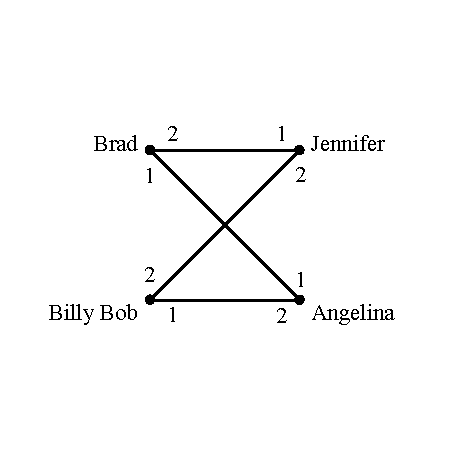
\includegraphics{minWtMatch2}

\caption{Preferences for four people.  Both men like Angelina best and
both women like Brad best.}
\label{fig:minWtMatch2}
\end{figure}

More generally, in any matching, a man and woman who are not married
to each other and who like each other better than their spouses, is
called a \emph{rogue couple}.  In the situation shown in
Figure~\ref{fig:minWtMatch2}, Brad and Angelina would be a rogue
couple.

Having a rogue couple is not a good thing, since it threatens the
stability of the marriages.  On the other hand, if there are no rogue
couples, then for any man and woman who are not married to each other,
at least one likes their spouse better than the other, and so they
won't be tempted to start an affair.

\begin{definition}
  A \term{stable matching} is a matching with no rogue couples.
\end{definition}

The question is, given everybody's preferences, how do you find a
stable set of marriages?  In the example consisting solely of the four
people in Figure~\ref{fig:minWtMatch2}, we could let Brad and Angelina
both have their first choices by marrying each other.  Now neither
Brad nor Angelina prefers anybody else to their spouse, so neither
will be in a rogue couple.  This leaves Jen not-so-happily married to
Billy Bob, but neither Jen nor Billy Bob can entice somebody else to
marry them, and so there is a stable matching.

Surprisingly, there always is a stable matching among a group of men
and women.  The surprise springs in part from considering the
apparently similar ``buddy'' matching problem.  That is, if people can
be paired off as buddies, regardless of gender, then a stable matching
\emph{may not} be possible.  For example, Figure~\ref{fig:buddy} shows
a situation with a love triangle and a fourth person who is everyone's
last choice.  In this figure Mergatroid's preferences aren't shown
because they don't even matter.  Let's see why there is no stable
matching.

\begin{figure}[htbp]

\redrawn

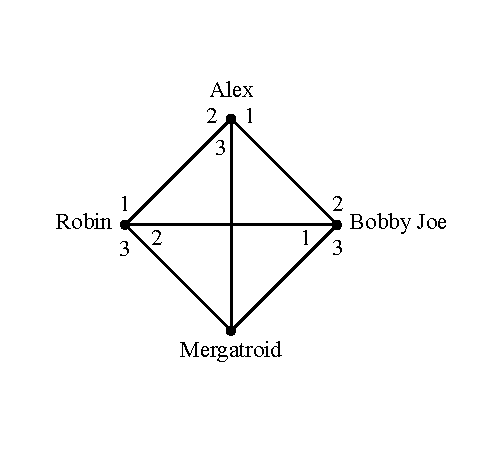
\includegraphics{loveTriangle}

\caption{Some preferences with no stable buddy matching.}
\label{fig:buddy}
\end{figure}

\begin{lemma}\label{lem:nostablematch}
There is no stable buddy matching among the four people in
Figure~\ref{fig:buddy}.
\end{lemma}

\begin{proof}
We'll prove this by contradiction.

Assume, for the purposes of contradiction, that there is a stable
matching.  Then there are two members of the love triangle that are
matched.  Since preferences in the triangle are symmetric, we may assume
in particular, that Robin and Alex are matched.  Then the other pair must
be Bobby-Joe matched with Mergatroid.

But then there is a rogue couple: Alex likes Bobby-Joe best, and Bobby-Joe
prefers Alex to his buddy Mergatroid.  That is, Alex and Bobby-Joe are a
rogue couple, contradicting the assumed stability of the matching.
\end{proof}

So getting a stable \emph{buddy} matching may not only be hard, it may
be impossible.  But when mens are only allowed to marry women, and
vice versa, then it turns out that a stable matching can always be
found.\footnote{Once again, we disclaim any political statement
  here---its just the way that the math works out.}

%%insert rest of story from gusfield book pp3--4??

\iffalse

\subsection{Failed attempts}

Let's find a stable matching in one possible situation, and hope to
translate our method to a general algorithm.  The table below shows the
preferences of each woman and man in decreasing order.

\begin{eqnarray*}
men & \quad & women \\
1 : C B E A D & \quad & A : 3 5 2 1 4 \\
2 : A B E C D & \quad & B : 5 2 1 4 3 \\
3 : D C B A E & \quad & C : 4 3 5 1 2 \\
4 : A C D B E & \quad & D : 1 2 3 4 5 \\
5 : A B D E C & \quad & E : 2 3 4 1 5
\end{eqnarray*}

How about we try a ``greedy'' strategy?\footnote{``Greedy'' is not any
moral judgment.  It refers to algorithms that work by always choosing the
next state that makes the largest immediate progress.}  We simply take
each man in turn and pack him off with his favorite among the women still
available.  This gives the following assignment.

\begin{eqnarray*}
1 \rightarrow C \\
2 \rightarrow A \\
3 \rightarrow D \\
4 \rightarrow B \\
5 \rightarrow E \\
\end{eqnarray*}

To determine whether this matching is stable, we have to check whether
there are any rogue couples.  Men 1, 2, and 3 all got their top pick
among the women; none would even think of running off.  Man~4 may be a
problem because he likes woman $A$ better than his mate, but she ranks him
dead last.  However, man~4 also likes woman $C$ better than his mate, and
she rates him above her own mate.  Therefore, man~4 and woman $C$ form a
rogue couple!  The marriages are not stable.  We could try to make ad hoc
repairs, but we're really trying to develop a general strategy.

Another approach would be to use induction.  Suppose we pair Man~1
with his favorite woman, $C$, try to show that neither of these two
will be involved in a rogue couple, and then solve the remaining
problem by induction.  Clearly Man~1 will never leave his top pick,
Woman $C$.  But the problem with this approach is that we \emph{can't}
be sure that Woman $C$ won't be in a rogue couple.  Woman $C$ might very
well dump Man~1---she might even rate him last!

This turns out to be a tricky problem.  The best approach is to use a
mating ritual that is reputed to have been popular in some mythic past.
\fi

\subsubsection{The Mating Ritual}

The procedure for finding a stable matching involves a \emph{Mating
Ritual} that takes place over several days.  The following events happen
each day:

\textbf{Morning}: Each woman stands on her balcony.  Each man stands
under the balcony of his favorite among the women on his list, and he
serenades her.  If a man has no women left on his list, he stays home
and does his math homework.

\textbf{Afternoon}: Each woman who has one or more suitors serenading
her, says to her favorite among them, ``We might get engaged.  Come
back tomorrow.''  To the other suitors, she says, ``No.  I will never
marry you!  Take a hike!''

\textbf{Evening}: Any man who is told by a woman to take a hike,
crosses that woman off his list.

\textbf{Termination condition}: When a day arrives in which every
woman has at most one suitor, the ritual ends with each woman marrying
her suitor, if she has one.

% Show example

There are a number of facts about this Mating Ritual that we would like to
prove:

\begin{itemize}
\item The Ritual eventually reaches the termination condition.
\item Everybody ends up married.
\item The resulting marriages are stable.
\end{itemize}


\subsubsection{There is a Marriage Day}

It's easy to see why the Mating Ritual has a terminal day when people
finally get married.  Every day on which the ritual hasn't terminated, at
least one man crosses a woman off his list.  (If the ritual hasn't
terminated, there must be some woman serenaded by at least two men, and at
least one of them will have to cross her off his list).  If we start with
$n$ men and $n$ women, then each of the $n$ men's lists initially has $n$
women on it, for a total of $n^2$ list entries.  Since no women ever gets
added to a list, the total number of entries on the lists decreases every
day that the Ritual continues, and so the Ritual can continue for at most
$n^2$ days.

\subsubsection{They All Live Happily Every After\dots}

We still have to prove that the Mating Ritual leaves everyone in a
stable marriage.  To do this, we note one very useful fact about the
Ritual: if a woman has a favorite suitor on some morning of the
Ritual, then that favorite suitor will still be serenading her the
next morning---because his list won't have changed.  So she is sure to
have today's favorite man among her suitors tomorrow.  That means she
will be able to choose a favorite suitor tomorrow who is at least as
desirable to her as today's favorite.  So day by day, her favorite
suitor can stay the same or get better, never worse.  This sounds like
an invariant, and it is.

\begin{definition}\label{def:P8}
Let $P$ be the predicate: For every woman, $w$, and every man, $m$, if
$w$ is crossed off $m$'s list, then $w$ has a suitor whom she prefers
over~$m$.
\end{definition}

\begin{lemma}\label{lem:5P}
$P$ is an invariant for The Mating Ritual.
\end{lemma}

\begin{proof}
By induction on the number of days.

\inductioncase{Base Case}: In the beginning (\ie at the end of day~0),
  every woman is on every list---no one has been crossed off and so
  $P$ is vacuously true.

\inductioncase{Inductive Step}: Assume $P$ is true at the end of
day~$d$ and let $w$ be a woman that has been crossed off a man $m$'s
list by the end of day~$d + 1$.

\begin{description}

\item[Case 1:]
$w$ was crossed off $m$'s list on day $d + 1$.  Then, $w$ must have a
  suitor she prefers on day~$d+1$.

\item[Case 2:]
$w$ was crossed off $m$'s list prior to day~$d+1$.  Since $P$ is true
  at the end of day~$d$, this means that $w$ has a suitor she prefers
  to~$m$ on day~$d$.  She therefore has the same suitor or someone she
  prefers better at the end of day~$d + 1$.

\end{description}
In both cases, $P$ is true at the end of day~$d + 1$ and so $P$ must
be an invariant.
\end{proof}

With Lemma~\ref{lem:5P} in hand, we can now prove:

\begin{theorem}
Everyone is married by the Mating Ritual.
\end{theorem}

\begin{proof}
By contradiction. Assume that it is the last day of the Mating Ritual
and someone does not get married.  Since there are an equal number of
men and women, and since bigamy is not allowed, this means that at
least one man (call him Bob) and at least one woman do not get
married.

Since Bob is not married, he can't be serenading anybody and so his
list must be empty.  This means that Bob has crossed every woman off
his list and so, by invariant~$P$, every woman has a suitor whom she
prefers to Bob.  Since it is the last day and every woman still has a
suitor, this means that every woman gets married.  This is a
contradiction since we already argued that at least one woman is
\emph{not} married.  Hence our assumption must be false and so
everyone must be married.
\end{proof}

\begin{theorem}
The Mating Ritual produces a stable matching.
\end{theorem}

\begin{proof}
Let Brad and Jen be any man and woman, respectively, that are
\emph{not} married to each other on the last day of the Mating Ritual.
We will prove that Brad and Jen are not a rogue couple, and thus that
all marriages on the last day are stable.  There are two cases to consider.
\begin{description}

\item[Case 1:] Jen is not on Brad's list by the end.  Then by invariant
  $P$, we know that Jen has a suitor (and hence a husband) that she
  prefers to Brad.  So she's not going to run off with Brad---Brad and
  Jen cannot be a rogue couple.

\item[Case 2:] Jen is on Brad's list.  But since Brad is not married to
  Jen, he must be choosing to serenade his wife instead of Jen, so he
  must prefer his wife.  So he's not going to run off with Jen---once
  again, Brad and Jenn are not a rogue couple.
 \qedhere

\end{description}

\end{proof}


\subsubsection{\dots Especially the Men}

Who is favored by the Mating Ritual, the men or the women?  The women
\emph{seem} to have all the power: they stand on their balconies
choosing the finest among their suitors and spurning the rest.  What's
more, we know their suitors can only change for the better as the
Ritual progresses.  Similarly, a man keeps serenading the woman he
most prefers among those on his list until he must cross her off, at
which point he serenades the next most preferred woman on his list.  So
from the man's perspective, the woman he is serenading can only change
for the worse.  Sounds like a good deal for the women.

But it's not!  The fact is that from the beginning, the men are
serenading their first choice woman, and the desirability of the woman
being serenaded decreases only enough to ensure overall stability.
The Mating Ritual actually does as well as possible for all the men
and does the worst possible job for the women.

To explain all this we need some definitions.  Let's begin by
observing that while The Mating Ritual produces one stable matching,
there may be other stable matchings among the same set of men and
women.  For example, reversing the roles of men and women will often
yield a different stable matching among them.

But some spouses might be out of the question in all possible stable
matchings.  For example, given the preferences shown in
Figure~\ref{fig:minWtMatch2}, Brad is just not in the realm of
possibility for Jennifer, since if you ever pair them, Brad and
Angelina will form a rogue couple.

\begin{definition}
Given a set of preference lists for all men and women, one person is
in another person's \emph{realm of possible spouses} if there is a
stable matching in which the two people are married.  A person's
\term{optimal spouse} is their most preferred person within their
realm of possibility.  A person's \term{pessimal spouse} is their
least preferred person in their realm of possibility.
\end{definition}

Everybody has an optimal and a pessimal spouse, since we know there is at
least one stable matching, namely, the one produced by the Mating Ritual.
Now here is the shocking truth about the Mating Ritual:

\begin{theorem}\label{boyopt}
The Mating Ritual marries every man to his optimal spouse.
\end{theorem}

\begin{proof}
By contradiction.  Assume for the purpose of contradiction that some
man does not get his optimal spouse.  Then there must have been a day
when he crossed off his optimal spouse---otherwise he would still be
serenading (and would ultimately marry) her or some even more
desirable woman.

By the Well Ordering Principle, there must be a \emph{first} day when
a man (call him ``Keith'') crosses off his optimal spouse (call her
Nicole).
According to the rules of the Ritual, Keith crosses off Nicole because
Nicole has a preferred suitor (call him Tom), so
\begin{equation}
\text{Nicole prefers Tom to Keith.} \tag{$*$}
\end{equation}

Since this is the first day an optimal woman gets crossed off, we know
that Tom had not previously crossed off his optimal spouse, and so
\begin{equation}\tag{$**$}
\text{Tom ranks Nicole at least as high as his optimal spouse.}
\end{equation}
By the definition of an optimal spouse, there must be some stable set
of marriages in which Keith gets his optimal spouse, Nicole.  But then
the preferences given in~($*$) and~($**$) imply that Nicole and Tom
are a rogue couple within this supposedly stable set of marriages
(think about it).  This is a contradiction.
\end{proof}

\begin{theorem}
The Mating Ritual marries every woman to her pessimal spouse.
\end{theorem}

\begin{proof}
By contradiction.  Assume that the theorem is not true.  Hence there
must be a stable set of marriages~$\mathcal{M}$ where some woman (call
her Nicole) is married to a man (call him Tom) that she likes less
than her spouse in The Mating Ritual (call him Keith).  This means
that
\begin{equation}
\text{Nicole prefers Keith to Tom.} \tag{+}
\end{equation}

By Theorem~\ref{boyopt} and the fact that Nicole and Keith are married
in the Mating Ritual, we know that 
\begin{equation}\tag{++}
\text{Keith prefers Nicole to his spouse in~$\mathcal{M}$.}
\end{equation}
This means that Keith and Nicole form a rogue couple in~$\mathcal{M}$,
which contradicts the stability of~$\mathcal{M}$.
\end{proof}

\subsubsection{Applications}

The Mating Ritual was first announced in a paper by D. \idx{Gale} and
L.S. \idx{Shapley} in 1962, but ten years before the Gale-Shapley
paper was published, and unknown by them, a similar algorithm was
being used to assign residents to hospitals by the National Resident
Matching Program (NRMP)\footnote{Of course, there is no serenading
  going on in the hospitals---the preferences are submitted to a
  program and the whole process is carried out by a computer.}.  The
NRMP has, since the turn of the twentieth century, assigned each
year's pool of medical school graduates to hospital residencies
(formerly called ``internships'') with hospitals and graduates playing
the roles of men and women.  (In this case, there may be multiple
women married to one man, a scenario we consider in the problem
section at the end of the chapter.).  Before the Ritual-like algorithm
was adopted, there were chronic disruptions and awkward
countermeasures taken to preserve assignments of graduates to
residencies.  The Ritual resolved these problems so successfully, that
it was used essentially without change at least through
1989.\footnote{Much more about the Stable Marriage Problem can be
  found in the very readable mathematical monograph by Dan Gusfield
  and Robert W. Irving,
  \href{http://mitpress.mit.edu/catalog/item/default.asp?ttype=2&tid=7676}{The
    Stable Marriage Problem: Structure and Algorithms}, MIT Press,
  Cambridge, Massachusetts, 1989, 240 pp.}

The Internet infrastructure company, Akamai, also uses a variation of
the Mating Ritual to assign web traffic to its servers.  In the early
days, Akamai used other combinatorial optimization algorithms that got
to be too slow as the number of servers (over 65,000 in 2010) and
requests (over 800 billion per day) increased.  Akamai switched to a
Ritual-like approach since it is fast and can be run in a distributed
manner.  In this case, web requests correspond to women and web
servers correspond to men.  The web requests have preferences based on
latency and packet loss, and the web servers have preferences based on
cost of bandwidth and colocation.

Not surprisingly, the Mating Ritual is also used by at least one large
online dating agency.  Even here, there is no serenading going
on---everything is handled by computer.

\begin{problems}

\practiceproblems

\pinput{CP_mating_ritual_example}

\pinput{TP_mating_ritual_invariant}

\classproblems

\pinput{CP_mating_ritual_proof}

\pinput{CP_stable_matching_non_optimal}

\homeworkproblems

\pinput{PS_stable_matching_hospitals}

\pinput{PS_stable_matching_no_first_choice}

\pinput{PS_stable_matching_unlucky}

\begin{editingnotes}
\begin{problem*}
Add problem proving that the Mating Ritual need not proceed in
morning/afternoon/evening lock step: a woman can reject non-favorite
suitors one at a time and at any time, and a rejected man can change
the woman he serenades without waiting for the other men to change.
The proof uses the fact that single actions commute, so induction
proves that all executions are confluent---which implies all
executions end with the same man-optimal matching.  This lemma can be
cited in the planar graphs section to prove that the edges in an
embedding can be added in any order.
\end{problem*}
\end{editingnotes}

\end{problems}

\section{Coloring}\label{sec:coloring}

In Section~\ref{sexam}, we used edges to indicate an affinity between
a pair of nodes.  We now consider situations where it is useful to use
edges to represent a \emph{conflict} between a pair of nodes.  For
example, consider the following exam scheduling problem.

\subsection{An Exam Scheduling Problem}

Each term, the MIT Schedules Office must assign a time slot for each
final exam.  This is not easy, because some students are taking
several classes with finals, and (even at MIT) a student can take only
one test during a particular time slot.  The Schedules Office wants to
avoid all conflicts.  Of course, you can make such a schedule by
having every exam in a different slot, but then you would need
hundreds of slots for the hundreds of courses, and the exam period
would run all year!  So, the Schedules Office would also like to keep
exam period short.

The Schedules Office's problem is easy to describe as a graph.  There
will be a vertex for each course with a final exam, and two vertices
will be adjacent exactly when some student is taking both courses.
For example, suppose we need to schedule exams for 6.041, 6.042,
6.002, 6.003 and 6.170.  The scheduling graph might appear as in
Figure~\ref{fig:5R}.

\begin{figure}

\redrawn

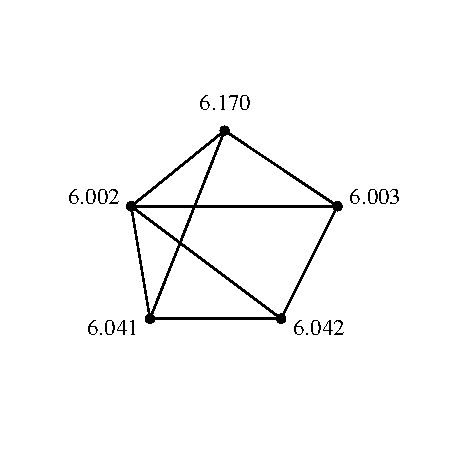
\includegraphics{finals-subject-labels}

\caption{A scheduling graph for five exams.  Exams connected by an
  edge cannot be given at the same time.}

\label{fig:5R}

\end{figure}

6.002 and 6.042 cannot have an exam at the same time since there are
students in both courses, so there is an edge between their nodes.  On the
other hand, 6.042 and 6.170 can have an exam at the same time if they're
taught at the same time (which they sometimes are), since no student can
be enrolled in both (that is, no student \emph{should} be enrolled in both
when they have a timing conflict).

We next identify each time slot with a color.  For example, Monday
morning is red, Monday afternoon is blue, Tuesday morning is green,
etc.  Assigning an exam to a time slot is then equivalent to coloring
the corresponding vertex.  The main constraint is that \emph{adjacent
  vertices must get different colors}---otherwise, some student has
two exams at the same time.  Furthermore, in order to keep the exam
period short, we should try to color all the vertices using as
\emph{few different colors as possible}.  As shown in Figure~\ref{fig:5S},
three colors suffice for our example.

\begin{figure}

\redrawn

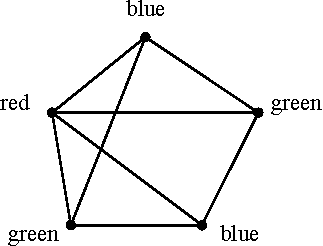
\includegraphics{finals-subject-colored}

\caption{A 3-coloring of the exam graph from Figure~\ref{fig:5R}.}

\label{fig:5S}

\end{figure}

The coloring in Figure~\ref{fig:5S} corresponds to giving one final on
Monday morning (red), two Monday afternoon (blue), and two Tuesday
morning (green).  Can we use fewer than three colors?  No! We can't
use only two colors since there is a triangle in the graph, and three
vertices in a triangle must all have different colors.

This is an example of a \term{graph coloring problem}: given a graph
$G$, assign colors to each node such that adjacent nodes have
different colors.  A color assignment with this property is called a
\term{valid coloring} of the graph---a ``\term{coloring},'' for short.
A graph $G$ is $k$-\term{colorable} if it has a coloring that uses at
most $k$ colors.
\begin{definition}
  The minimum value of $k$ for which a graph, $G$, has a valid coloring is
  called its \term{chromatic number}, $\chi(G)$.
\end{definition}

In general, trying to figure out if you can color a graph with a fixed
number of colors can take a long time.  It's a classic example of a
problem for which no fast algorithms are known.  In fact, it is easy to
check if a coloring works, but it seems really hard to find it. (If you
figure out how, then you can get a \$1 million Clay prize.)


\subsection{Some Coloring Bounds}

There are some simple properties of graphs that give useful upper bounds
on the chromatic number.  For example, if a graph is bipartite, then we
can color it with 2 colors---one color for the nodes in the ``left'' set
and a second color for the nodes in the ``right'' set.  Conversely, if a
graph is 2-colorable, then it is bipartite: let the ``left'' vertices be
the ones with one color and the ``right'' vertices the ones with the other
color.  In other words, being bipartite is equivalent to being
2-colorable.

Planarity is another property with important colorability consequences.
The famous 4-Color Theorem says that every planar graph is 4-colorable.
This is a hard result to prove, but we will come close in
Section~\ref{planar_graphs_sec} where we define planar graphs and prove
that they are 5-colorable.

The chromatic number of a graph can also be shown to be small if the
vertex degrees of the graph are small.  In particular, if we have an
upper bound on the degrees of all the vertices in a graph, then we can
easily find a coloring with only one more color than the degree bound.

\begin{theorem}\label{k+1-colorable}
A graph with maximum degree at most $k$ is $(k+1)$-colorable.
\end{theorem}

The natural way to try to prove this theorem is to use induction
on~$k$.  Unfortunately, this approach leads to disaster.  It is not
that it is impossible, just that it is extremely painful and would
ruin your week if you tried it on an exam.  When you encounter such a
disaster when using induction on graphs, it is usually best to change
what you are inducting on.  In graphs, typical good choices for the
induction parameter are $n$, the number of nodes, or $e$, the number
of edges.

\begin{proof}[Proof of Theorem~\ref{k+1-colorable}]
We use induction on the number of vertices in the graph, which we
denote by $n$.  Let $P(n)$ be the proposition that an $n$-vertex graph
with maximum degree at most $k$ is $(k+1)$-colorable.

\inductioncase{Base case} ($n=1$): A 1-vertex graph has maximum degree
0 and is 1-colorable, so $P(1)$ is true.

\inductioncase{Inductive step}: Now assume that $P(n)$ is true, and
let $G$ be an $(n+1)$-vertex graph with maximum degree at most $k$.
Remove a vertex $v$ (and all edges incident to it), leaving an
$n$-vertex subgraph, $H$.  The maximum degree of $H$ is at most $k$,
and so $H$ is $(k+1)$-colorable by our assumption $P(n)$.  Now add
back vertex $v$.  We can assign $v$ a color (from the set of $k + 1$
colors) that is different from all its adjacent vertices, since there
are at most $k$ vertices adjacent to~$v$ and so at least one of the
$k+1$ colors is still available.  Therefore, $G$ is $(k+1)$-colorable.
This completes the inductive step, and the theorem follows by
induction.
\end{proof}

Sometimes $k+1$ colors is the best you can do.  For example, in the
complete graph, $K_n$, every one of its $n$ vertices is adjacent to
all the others, so all $n$ must be assigned different colors.  Of
course $n$ colors is also enough, so $\chi(K_n)=n$.  In this case,
every node has degree $k = n - 1$ and so this is an example where
Theorem~\ref{k+1-colorable} gives the best possible bound.  By a
similar argument, we can show that Theorem~\ref{k+1-colorable} gives
the best possible bound for \emph{any} graph with degree bounded by
$k$ that has $K_{k+1}$ as a subgraph.

But sometimes $k+1$ colors is far from the best that you can do.
For example, the $n$-node \emph{star graph} shown in
Figure~\ref{fig:5T} has maximum degree $n - 1$ but can be colored
using just 2 colors.

\begin{figure}

\redrawn

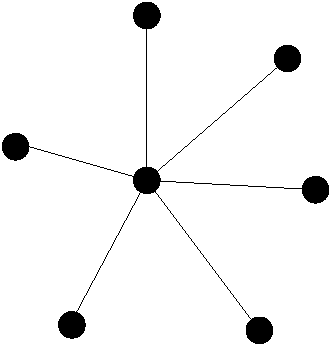
\includegraphics{star-graph}

\caption{A 7-node star graph.}

\label{fig:5T}

\end{figure}


\subsection{Why coloring?}

One reason coloring problems frequently arise in practice is because
scheduling conflicts are so common.  For example, at Akamai, a new
version of software is deployed over each of 65,000 servers every few
days.  The updates cannot be done at the same time since the servers
need to be taken down in order to deploy the software.  Also, the
servers cannot be handled one at a time, since it would take forever
to update them all (each one takes about an hour).  Moreover, certain
pairs of servers cannot be taken down at the same time since they have
common critical functions.  This problem was eventually solved by
making a 65,000-node conflict graph and coloring it with 8 colors---so
only 8 waves of install are needed!

Another example comes from the need to assign frequencies to radio
stations.  If two stations have an overlap in their broadcast area, they
can't be given the same frequency.  Frequencies are precious and
expensive, so you want to minimize the number handed out.  This amounts to
finding the minimum coloring for a graph whose vertices are the stations
and whose edges connect stations with overlapping areas.

Coloring also comes up in allocating registers for program variables.
While a variable is in use, its value needs to be saved in a register.
Registers can be reused for different variables but two variables need
different registers if they are referenced during overlapping
intervals of program execution.  So register allocation is the
coloring problem for a graph whose vertices are the variables;
vertices are adjacent if their intervals overlap, and the colors are
registers.  Once again, the goal is to minimize the number of colors
needed to color the graph.

Finally, there's the famous map coloring problem stated in
Proposition~\ref{4colorprop}.  The question is how many colors are needed
to color a map so that adjacent territories get different colors?  This is
the same as the number of colors needed to color a graph that can be drawn
in the plane without edges crossing.  A proof that four colors are enough
for \index{planar graphs} \emph{planar} graphs was acclaimed when it was
discovered about thirty years ago.  Implicit in that proof was a
4-coloring procedure that takes time proportional to the number of
vertices in the graph (countries in the map).  Surprisingly, it's another
of those million dollar prize questions to find an efficient procedure to
tell if a planar graph really \emph{needs} four colors or if three will
actually do the job.  (It's always easy to tell if an \emph{arbitrary}
graph is 2-colorable.)  In Section~\ref{planar_graphs_sec}, we'll develop
enough planar graph theory to present an easy proof that all planar graphs
are 5-colorable.

%% Connectedness %%%%%%%%%%%%%%%%%%%%%%%%%%%%%%%%%%%%%%%%%%%%%%%%%%%%%%%%%%%%%%

\section{Getting from $A$ to~$B$ in a Graph}\label{sec:connectedness}

\subsection{Paths and Walks}

\begin{definition}\label{def:undirected-path}
A \term{walk}\footnote{Some texts use the word \emph{path} for our
  definition of walk and the term \emph{simple path} for our
  definition of path.} in a graph, $G$, is a sequence of vertices
\begin{equation*}
v_0, v_1, \dots, v_k
\end{equation*}
and edges
\begin{equation*}
    \edge{v_0}{v_1}, \edge{v_1}{v_2}, \dots, \edge{v_{k - 1}}{v_k}
\end{equation*}
such that $\edge{v_i}{v_{i+1}}$ is an edge of $G$ for all $i$ where $0
\leq i < k$ .  The walk is said to \index{start of path}\emph{start}
at $v_0$ and to \index{end of walk}\emph{end} at $v_k$, and the
\index{length of walk}\emph{length} of the walk is defined to be $k$.
An edge, $\edge{u}{v}$, is \term{traversed} $n$ times by the walk if
there are $n$ different values of $i$ such that $\edge{v_i}{v_{i+1}} =
\edge{u}{v}$.  A \emph{path} is a walk where all the $v_i$'s are
different, that is, $i\neq j$ implies $v_i \neq v_j$.  For simplicity,
we will refer to paths and walks by the sequence of
vertices.\footnote{This works fine for simple graphs since the edges
  in a walk are completely determined by the sequence of vertices and
  there is no ambiguity.  For graphs with multiple edges, we would
  need to specify the edges as well as the nodes.}
\end{definition}

For example, the graph in Figure~\ref{dg} has a length~6 path $a$,
$b$, $c$, $d$, $e$, $f$,~$g$.  This is the longest path in the graph.
Of course, the graph has walks with arbitrarily large lengths, for
example, $a$, $b$, $a$, $b$, $a$, $b$,\dots.
\begin{figure}[htbp]

\redrawn

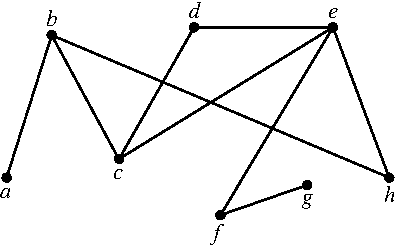
\includegraphics{distance-graph}

\caption{A graph containing a path $a$, $b$, $c$, $d$, $e$, $f$,~$g$
  of length~6.}
\label{dg}
\end{figure}

The length of a walk or path is the total number of times it traverses
edges, which is \emph{one less} than its length as a sequence of
vertices.  For example, the length~6 path $a$, $b$, $c$, $d$, $e$,
$f$,~$g$ contains a sequence of 7~vertices.

\subsection{Finding a Path}

Where there's a walk, there's a path.  This is sort of obvious, but
it's easy enough to prove rigorously using the \idx{Well Ordering
  Principle}.

\begin{lemma}\label{simplepath}
If there is a walk from a vertex $u$ to a vertex~$v$ in a graph, then
there is a path from $u$ to~$v$.
\end{lemma}

\begin{proof}
Since there is a walk from $u$ to $v$, there must, by the
Well-ordering Principle, be a minimum length walk from $u$ to~$v$.  If
the minimum length is zero or one, this minimum length walk is itself
a path from $u$ to $v$.  Otherwise, there is a minimum length walk
\[
v_0, v_1, \dots, v_k
\]
from $u = v_0$ to $v = v_k$ where $k \geq 2$.  We claim this walk must
be a path.  To prove the claim, suppose to the contrary that the walk
is not a path; that is, some vertex on the walk occurs twice.  This
means that there are integers $i,j$ such that $0 \leq i < j \leq k$
with $v_i= v_j$.  Then deleting the subsequence
\[
    v_{i+1}, \dots, v_j
\]
yields a strictly shorter walk
\[
    v_0, v_1,\dots, v_i,v_{j+1},v_{j+2},\dots, v_k
\]
from $u$ to $v$, contradicting the minimality of the given walk.
\end{proof}

Actually, we proved something stronger:
\begin{corollary}\label{ss}
For any walk of length $k$ in a graph, there is a path of length
\emph{at most} $k$ with the same endpoints.  Moreover, the shortest
walk between a pair of vertices is, in fact, a path.
\end{corollary}

\subsection{Numbers of Walks}

Given a pair of nodes that are connected by a walk of length~$k$ in a
graph, there are often many walks that can be used to get from one
node to the other.  For example, there are 5 walks of length~3 that
start at~$v_1$ and end at~$v_4$ in the graph shown in
Figure~\ref{fig:5AD}.

\begin{figure}

\redrawn

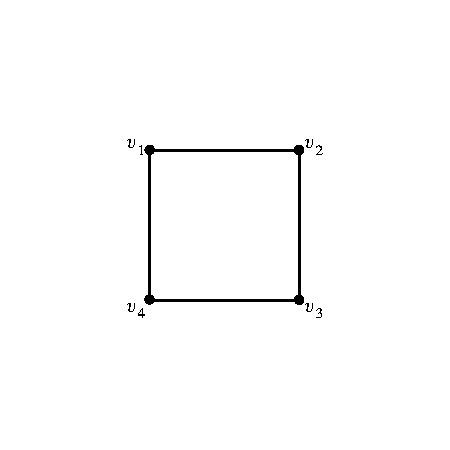
\includegraphics{Fig_5AD}

\caption{A graph for which there are 5 walks of length~3 from $v_1$
  to~$v_4$.  The walks are $(v_1, v_2, v_1, v_4)$, $(v_1, v_3, v_1,
  v_4)$, $(v_1, v_4, v_1, v_4)$, $(v_1, v_2, v_3, v_4)$, and $(v_1,
  v_4, v_3, v_4)$.}
\label{fig:5AD}
\end{figure}

There is a surprising relationship between the number of walks of
length~$k$ between a pair of nodes in a graph~$G$ and the $k$th power
of the adjacency matrix~$A_G$ for~$G$.  The relationship is captured
in the following theorem.

\begin{theorem}\label{thm:5AE}
Let $G$ be an $n$-node graph with $\vertices{G} = \set{\, v_1, v_2, \dots,
v_n\, }$ and let $A_G = \set{ a_{ij} }$ denote the adjacency matrix
for~$G$.  Let $a_{ij}^{(k)}$ denote the $(i, j)$-entry of the $k$th
power of~$A_G$.  Then the number of walks of length~$k$ between $v_i$
and~$v_j$ is~$a_{ij}^{(k)}$.
\end{theorem}

In other words, we can determine the number of walks of length~$k$
between any pair of nodes simply by computing the $k$th power of the
adjacency matrix!  That's pretty amazing.

For example, the first three powers of the adjacency matrix for the
graph in Figure~\ref{fig:5AD} are:
\begin{align*}
    A &= \begin{pmatrix}
            0 & 1 & 1 & 1 \\
            1 & 0 & 1 & 0 \\
            1 & 1 & 0 & 1 \\
            1 & 0 & 1 & 0
         \end{pmatrix} & % \\[\medskipamount]
  A^2 &= \begin{pmatrix}
            3 & 1 & 2 & 1 \\
            1 & 2 & 1 & 2 \\
            2 & 1 & 3 & 1 \\
            1 & 2 & 1 & 2
         \end{pmatrix} & % \\[\medskipamount]
  A^3 &= \begin{pmatrix}
            4 & 5 & 5 & 5 \\
            5 & 2 & 5 & 2 \\
            5 & 5 & 4 & 5 \\
            5 & 2 & 5 & 2
         \end{pmatrix}
\end{align*}

Sure enough, the $(1, 4)$ coordinate of~$A^3$ is $a_{14}^{(3)} = 5$,
which is the number of length~3 walks from~$v_1$ to~$v_4$.  And
$a_{24}^{(3)} = 2$, which is the number of length~3 walks from $v_2$
to~$v_4$.  By proving the theorem, we'll discover why it is true and
thereby uncover the relationship between matrix multiplication and
numbers of walks.

\begin{proof}[Proof of Theorem~\ref{thm:5AE}]
The proof is by induction on~$k$.  We will let $P(k)$ be the predicate
that the theorem is true for~$k$.  Let $P_{ij}^{(k)}$ denote the
number of walks of length~$k$ between $v_i$ and~$v_j$.  Then $P(k)$ is
the predicate
\begin{equation}\label{eq:5AE}
    \forall i, j \in [1, n].\; P_{ij}^{(k)} = a_{ij}^{(k)}.
\end{equation}

\inductioncase{Base Case} ($k = 1$):  There are two cases to consider:
\begin{description}

\item[Case 1:]

$\{ v_i, v_j \} \in E$.  Then $P_{ij}^{(1)} = 1$ since there is
  precisely one walk of length~1 between $v_i$ and~$v_j$.  Moreover,
  $\{ v_i, v_j \} \in E$ means that $a_{ij}^{(1)} = a_{ij} = 1$.  So,
  $P_{ij}^{(1)} = a_{ij}^{(1)}$ in this case.

\item[Case 2:]

$\{ v_i, v_j \} \notin E$.  Then $P_{ij}^{(1)} = 0$ since there
  cannot be any walks of length~1 between $v_i$ and~$v_j$.  Moreover,
  $\{ v_i, v_j \} \notin E$ means that $a_{ij} = 0$.  So,
  $P_{ij}^{(1)} = a_{ij}^{(1)}$ in this case as well.

\end{description}

Hence, $P(1)$ must be true.

\inductioncase{Inductive Step}:
Assume $P(k)$ is true.  In other words, assume that
equation~\ref{eq:5AE} holds.

We can group (and thus count the number of) walks of length $k+1$
from $v_i$ to~$v_j$ according to the first edge in the walk (call it
$\{ v_i, v_t \}$).  This means that
\begin{equation}\label{eq:5AF}
    P_{ij}^{(k + 1)} = \sum^{t: \{ v_i, v_t \} \in E} P_{tj}^{(k)}
\end{equation}
where the sum is over all~$t$ such that $\{ v_i, v_t \}$ is an edge.
Using the fact that $a_{ij} = 1$ if $\{ v_i, v_t \} \in E$ and $a_{it}
= 0$ otherwise, we can rewrite Equation~\ref{eq:5AF} as follows:
\begin{equation*}
    P_{ij}^{(k + 1)} = \sum_{t = 1}^{n} a_{it} P_{tj}^{(k)}.
\end{equation*}
By the inductive hypothesis, $P_{tj}^{(k)} = a_{tj}^{(k)}$ and thus
\begin{equation*}
    P_{ij}^{(k + 1)} = \sum_{t = 1}^{n} a_{it} a_{tj}^{(k)}.
\end{equation*}
But the formula for matrix multiplication gives that
\begin{equation*}
    a_{ij}^{(k + 1)} = \sum_{t = 1}^{n} a_{it} a_{tj}^{(k)}.
\end{equation*}
and so we must have $P_{ij}^{(k+1)} = a_{ij}^{(k+1)}$ for all $i, j
\in [1, n]$.  Hence $P(k+1)$ is true and the induction is complete.
\end{proof}

\subsection{Shortest Paths}

Although the connection between the power of the adjacency matrix and
the number of walks is cool (at least if you are a mathematician), the
problem of counting walks does not come up very often in practice.
Much more important is the problem of finding the shortest path
between a pair of nodes in a graph.

There is good news and bad news to report on this front.  The good
news is that it is not very hard to find a shortest path.  The bad
news is that you can't win one of those million dollar prizes for
doing it.

In fact, there are several good algorithms known for finding a
Shortest Path between a pair of nodes.  The simplest to explain (but
not the fastest) is to compute the powers of the adjacency matrix one
by one until the value of~$a_{ij}^{(k)}$ exceeds~0.  That's because
Theorem~\ref{thm:5AE} and Corollary~\ref{ss} imply that the length of
the shortest path between $v_i$ and~$v_j$ will be the smallest value
of~$k$ for which $a_{ij}^{(k)} > 0$.

\subsubsection{Paths in Weighted Graphs}

The problem of computing shortest paths in a weighted graph frequently
arises in practice. For example, when you drive home for vacation, you
usually would like to take the shortest route.

\begin{definition}\label{def:5H}
Given a weighted graph, the length of a path in the graph is the sum
of the weights of the edges in the path.
\end{definition}

Finding shortest paths in weighted graphs is not a lot harder than
finding shortest paths in unweighted graphs.  We won't show you how to
do it here, but you will study algorithms for finding shortest paths
if you take an algorithms course.  Not surprisingly, the proof of
correctness will use induction.

\section{Connectivity}

\begin{definition}
  Two vertices in a graph are said to be \term{connected} if there
  is a path that begins at one and ends at the other.  By convention,
  every vertex is considered to be connected to itself by a path of
  length zero.
\end{definition}

\begin{definition}\label{def:connected-graph}
A graph is said to be \term{connected} when every pair of vertices are
connected.
\end{definition}

\subsection{Connected Components}

Being connected is usually a good property for a graph to have.  For
example, it could mean that it is possible to get from any node to any
other node, or that it is possible to communicate between any pair of
nodes, depending on the application.

But not all graphs are connected.  For example, the graph where nodes
represent cities and edges represent highways might be connected for
North American cities, but would surely not be connected if you also
included cities in Australia.  The same is true for communication
networks like the Internet---in order to be protected from viruses
that spread on the Internet, some government networks are completely
isolated from the Internet.

\begin{figure}[htbp]

\redrawn

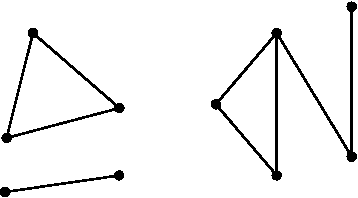
\includegraphics{connectivity-graphs}

\caption{One graph with 3 connected components.}

\label{fig:3comp}
\end{figure}

For example, the diagram in Figure~\ref{fig:3comp} looks like a
picture of three graphs, but is intended to be a picture of \emph{one}
graph.  This graph consists of three pieces (subgraphs).  Each piece
by itself is connected, but there are no paths between vertices in
different pieces.  These connected pieces of a graph are called its
\term{connected components}.

\begin{definition}\label{def:connected-component}
A \emph{connected component} is a subgraph of a graph consisting of
some vertex and every node and edge that is connected to that vertex.
\end{definition}

So a graph is connected iff it has exactly one connected component.
At the other extreme, the empty graph on $n$ vertices has $n$
connected components.

\subsection{$k$-Connected Graphs}

If we think of a graph as modeling cables in a telephone network, or
oil pipelines, or electrical power lines, then we not only want
connectivity, but we want connectivity that survives component
failure.  A graph is called \emph{$k$-edge connected} if it takes at
least $k$ ``edge-failures'' to disconnect it.  More precisely:

\begin{definition}
  Two vertices in a graph are $k$-\term{edge connected} if they remain
  connected in every subgraph obtained by deleting $k-1$ edges.  A graph
  with at least two vertices is $k$-edge connected\footnote{The
    corresponding definition of connectedness based on deleting vertices
    rather than edges is common in Graph Theory texts and is usually
    simply called ``$k$-connected'' rather than ``$k$-vertex connected.''}
  if every two of its vertices are $k$-edge connected.
\end{definition}

So 1-edge connected is the same as connected for both vertices and
graphs.  Another way to say that a graph is $k$-edge connected is
that every subgraph obtained from it by deleting at most $k-1$ edges
is connected.  For example, in the graph in Figure~\ref{dg},
vertices $c$ and~$e$ are 3-edge connected, $b$ and~$e$ are 2-edge
connected, $g$ and $e$ are 1-edge connected, and no vertices are
4-edge connected.  The graph as a whole is only 1-edge connected.
The complete graph, $K_n$, is $(n-1)$-edge connected.

If two vertices are connected by $k$ edge-disjoint paths (that is, no
two paths traverse the same edge), then they are obviously $k$-edge
connected.  A fundamental fact, whose ingenious proof we omit,
is \idx{Menger}'s theorem which confirms that the converse is also
true: if two vertices are $k$-edge connected, then there are $k$
edge-disjoint paths connecting them.  It even takes some ingenuity to
prove this for the case $k=2$.

\subsection{The Minimum Number of Edges in a Connected Graph}

The following theorem says that a graph with few edges must have many
connected components.
\begin{theorem}\label{th:connectivity}
Every graph with $v$ vertices and $e$ edges has at least $v - e$ connected
components.
\end{theorem}
Of course for Theorem~\ref{th:connectivity} to be of any use, there must
be fewer edges than vertices.

\begin{proof}
We use induction on the number of edges, $e$.  Let $P(e)$ be the
proposition that
\begin{quote}
for every $v$, every graph with $v$ vertices and $e$ edges has at least
$v-e$ connected components.
\end{quote}

\textbf{Base case:}($e=0$).  In a graph with 0 edges and $v$ vertices,
each vertex is itself a connected component, and so there are exactly $v =
v - 0$ connected components.  So $P(e)$ holds.

\textbf{Inductive step:} Now we assume that the induction hypothesis
holds for every $e$-edge graph in order to prove that it holds for
every $(e+1)$-edge graph, where $e \geq 0$.  Consider a graph, $G$,
with $e + 1$ edges and $v$ vertices.  We want to prove that $G$ has at
least $v - (e+1)$ connected components.  To do this, remove an
arbitrary edge $\edge{a}{b}$ and call the resulting graph $G'$.  By
the induction assumption, $G'$ has at least $v - e$ connected
components.  Now add back the edge $\edge{a}{b}$ to obtain the
original graph $G$.  If $a$ and $b$ were in the same connected
component of $G'$, then $G$ has the same connected components as $G'$,
so $G$ has at least $v -e > v - (e+1)$ components.  Otherwise, if $a$
and $b$ were in different connected components of $G'$, then these two
components are merged into one component in~$G$, but all other
components remain unchanged, reducing the number of components by 1.
Therefore, $G$ has at least $(v - e) - 1 = v - (e+1)$ connected
components.  So in either case, $P(e+1)$ holds.  This completes the
Inductive step.  The theorem now follows by induction.
\end{proof}

\begin{corollary}
\label{cor:n-1}
Every connected graph with $v$ vertices has at least $v - 1$ edges.
\end{corollary}

A couple of points about the proof of Theorem~\ref{th:connectivity}
are worth noticing.  First, we used induction on the number of edges
in the graph.  This is very common in proofs involving graphs, as is
induction on the number of vertices.  When you're presented with a
graph problem, these two approaches should be among the first you
consider.

The second point is more subtle.  Notice that in the inductive step,
we took an arbitrary $(n+1)$-edge graph, threw out an edge so that
we could apply the induction assumption, and then put the edge back.
You'll see this shrink-down, grow-back process very often in the
inductive steps of proofs related to graphs.  This might seem like
needless effort: why not start with an $n$-edge graph and add one
more to get an $(n+1)$-edge graph?  That would work fine in this
case, but opens the door to a nasty logical error called
\term{buildup error}.

\subsection{Build-Up Error}

\begin{falseclm*}
If every vertex in a graph has degree at least~1, then the graph is
connected.
\end{falseclm*}

There are many counterexamples; for example, see Figure~\ref{fig:5Z}.

\begin{figure}

\redrawn


\includegraphics{Fig_5Z}

\caption{A counterexample graph to the False Claim.}

\label{fig:5Z}
\end{figure}

\begin{falseproof}
We use induction.  Let $P(n)$ be the proposition that if every vertex
in an $n$-vertex graph has degree at least~1, then the graph is
connected.

\inductioncase{Base case}: There is only one graph with a single
vertex and has degree~0.  Therefore, $P(1)$ is vacuously true, since
the if-part is false.

\inductioncase{Inductive step}: We must show that $P(n)$ implies
$P(n+1)$ for all $n \ge 1$.  Consider an $n$-vertex graph in which
every vertex has degree at least~1.  By the assumption~$P(n)$, this
graph is connected; that is, there is a path between every pair of
vertices.  Now we add one more vertex~$x$ to obtain an $(n+1)$-vertex
graph as shown in Figure~\ref{fig:5Y}.

\begin{figure}

\redrawn

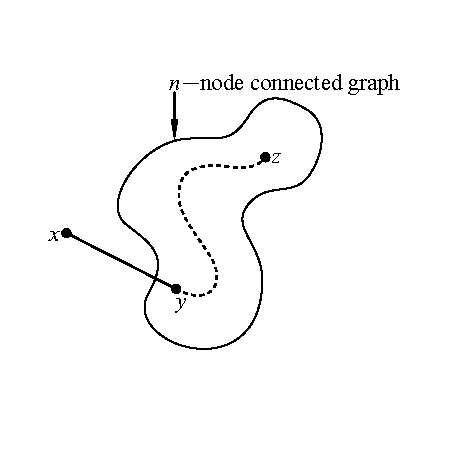
\includegraphics{false-connect-pic}

\caption{Adding a vertex~$x$ with degree at least~1 to a connected
  $n$-node graph.}

\label{fig:5Y}

\end{figure}

All that remains is to check that there is a path from $x$ to every
other vertex~$z$.  Since $x$ has degree at least one, there is an edge
from~$x$ to some other vertex; call it~$y$.  Thus, we can obtain a
path from~$x$ to~$z$ by adjoining the edge $\edge{x}{y}$ to the path
from~$y$ to~$z$.  This proves $P(n + 1)$.

By the principle of induction, $P(n)$ is true for all  $n \ge 1$,
which proves the theorem
\end{falseproof}

Uh-oh\dots this proof looks fine!  Where is the bug?  It turns out
that the faulty assumption underlying this argument is that
\emph{every $(n + 1)$-vertex graph with minimum degree~1 can be
obtained from an $n$-vertex graph with minimum degree~1 by adding 1
more vertex}.  Instead of starting by considering an arbitrary $(n +
1)$-node graph, this proof only considered $(n + 1)$-node graphs
that you can make by starting with an $n$-node graph with minimum
degree~1.

The counterexample in Figure~\ref{fig:5Z} shows that this assumption
is false; there is no way to build the 4-vertex graph in
Figure~\ref{fig:5Z} from a 3-vertex graph with minimum degree~1.
Thus the first error in the proof is the statement ``This proves
$P(n + 1)$.''

This kind of flaw is known as ``build-up error.''  Usually, build-up
error arises from a faulty assumption that every size $n + 1$ graph
with some property can be ``built up'' from a size~$n$ graph with the
same property.  (This assumption is correct for some properties, but
incorrect for others---such as the one in the argument above.)

One way to avoid an accidental build-up error is to use a ``shrink
down, grow back'' process in the inductive step: \ie start with a size
$n+1$ graph, remove a vertex (or edge), apply the inductive hypothesis
$P(n)$ to the smaller graph, and then add back the vertex (or edge)
and argue that $P(n + 1)$ holds.  Let's see what would have happened
if we'd tried to prove the claim above by this method:

\inductioncase{Revised inductive step}: We must show that $P(n)$
implies $P(n + 1)$ for all $n \ge 1$.  Consider an $(n + 1)$-vertex
graph~$G$ in which every vertex has degree at least~1.  Remove an
arbitrary vertex~$v$, leaving an $n$-vertex graph~$G'$ in which every
vertex has degree\dots\ uh oh!

The reduced graph~$G'$ might contain a vertex of degree~0, making the
inductive hypothesis $P(n)$ inapplicable!  We are stuck---and
properly so, since the claim is false!

Always use shrink-down, grow-back arguments and you'll never fall into
this trap.

%S08, cp6m, S06 cp5f

%S06 cp5f

%% Connectedness Problems %%%%%%%%%%%%%%%%%%%%%%%%%%%%%%%%%%%%%%%%%%%%%%%%%%%%
\begin{problems}
\classproblems
\pinput{CP_n_dim_hypercube}
\pinput{CP_graph_maximal_connected}
\pinput{CP_Kn_is_very_connected}
\pinput{CP_pos_deg_but_not_connected}
\homeworkproblems
\pinput{PS_Euler_circuits}

% S09.cp6m.2
% S09.cp6t.1

\homeworkproblems
\pinput{PS_tangled_and_mangled_graphs}
\pinput{PS_circuit_graph_with_crossbars}
\end{problems}

\section{Around and Around We Go}

\subsection{Cycles and Closed Walks}

\begin{definition}
A \emph{closed walk}\footnote{Some texts use the word \emph{cycle} for
  our definition of closed walk and \emph{simple cycle} for our
  definition of cycle.} in a graph~$G$ is a sequence of vertices
\begin{equation*}
    v_0, v_1, \dots, v_k
\end{equation*}
and edges
\begin{equation*}
    \edge{v_0}{v_1}, \edge{v_1}{v_2}, \dots, \edge{v_{k - 1}}{v_k}
\end{equation*}
where $v_0$ is the same node as~$v_k$ and $\edge{v_i}{v_{i + 1}}$ is
an edge of~$G$ for all~$i$ where $0 \le i < k$.  The \emph{length} of
the closed walk is~$k$.  A closed walk is said to be a \emph{cycle} if
$k \ge 3$ and $v_0$, $v_1$, \dots, $v_{k - 1}$ are all different.
\end{definition}

For example, $b$, $c$, $d$, $e$, $c$,~$b$ is a closed walk of
length~5 in the graph shown in Figure~\ref{dg}.  It is not a cycle
since it contains node~$c$ twice.  On the other hand, $c$, $d$,
$e$,~$c$ is a cycle of length~3 in this graph since every node
appears just once.

There are many ways to represent the same closed walk or cycle.  For
example, $b$, $c$, $d$, $e$, $c$,~$b$ is the same as $c$, $d$, $e$,
$c$, $b$,~$c$ (just starting at node~$c$ instead of node~$b$) and the
same as $b$, $c$, $e$, $d$, $c$,~$b$ (just reversing the direction).

Cycles are similar to paths, except that the last node is the first
node and the notion of first and last does not matter.  Indeed, there
are many possible vertex orders that can be used to describe cycles
and closed walks, whereas walks and paths have a prescribed beginning,
end, and ordering.

\begin{editingnotes}
\begin{staffnotes}This section seems tedious and unnecessary.
It was adequately covered in Problem~\ref{PS_no_odd_length_closed_walks}

\end{staffnotes}

\subsection*{Odd Cycles and 2-Colorability}

We have already seen that determining the chromatic number of a graph
is a challenging problem.  There is one special case where this
problem is very easy; namely, the case where every cycle in the graph
has even length.  In this case, the graph is 2-colorable!  Of course,
this is optimal if the graph has any edges at all.  More generally, we
will prove

\begin{theorem}\label{thm:XY}
The following properties of a graph are equivalent (that is, if the
graph has any one of the properties, then it has all of the
properties):
\begin{enumerate}

\item\label{thm:XY:i}
The graph is bipartite.

\item\label{thm:XY:ii}
The graph is 2-colorable.

\item\label{thm:XY:iii}
The graph does not contain any closed walks with odd length.

\item\label{thm:XY:iv}
The graph does not contain any cycles with odd length.

\end{enumerate}
\end{theorem}

\begin{proof}

We will show that
property~\ref{thm:XY:i} $\QIMPLIES$ property~\ref{thm:XY:ii}, 
property~\ref{thm:XY:ii} $\QIMPLIES$ property~\ref{thm:XY:iii}, 
property~\ref{thm:XY:iii} $\QIMPLIES$ property~\ref{thm:XY:iv}, and
property~\ref{thm:XY:iv} $\QIMPLIES$ property~\ref{thm:XY:i}.  This
will show that all four properties are equivalent by repeated
application of Rule~\ref{rule:transitivity} in
Section~\ref{sec:logical_deduction}.

\begin{description}

\item[\ref{thm:XY:i} $\QIMPLIES$ \ref{thm:XY:ii}]

Assume that $G = (V, E)$ is a bipartite graph.  Then $V$ can be
partitioned into two sets $L$ and~$R$ so that no edge connects a pair
of nodes in~$L$ nor a pair of nodes in~$R$.  Hence, we can use one
color for all the nodes in ~$L$ and a second color for all the nodes
in~$R$.  Hence $\chi(G) = 2$.

\item[\ref{thm:XY:ii} $\QIMPLIES$ \ref{thm:XY:iii}]

Let $G = (V, E)$ be a 2-colorable graph and
\begin{equation*}
    w ::= v_0, v_1, \dots, v_k
\end{equation*}
be any closed walk in~$G$.  Consider any 2-coloring for the nodes
of~$G$.  Since $\edge{v_i}{v_{i + 1}} \in E$, \ $v_i$ and $v_{i + 1}$
must be differently colored for $0 \le i < k$.  Hence $v_0$, $v_2$,
$v_4$, \dots, have one color and $v_1$, $v_3$, $v_5$, \dots, have the
other color.  Since $w$ is a closed walk, $v_k$ is the same node
as~$v_0$ and so $k$ must be an even number.  This means that $w$ has
even length.

\item[\ref{thm:XY:iii} $\QIMPLIES$ \ref{thm:XY:iv}]

Since every cycle is a closed walk, a graph without any odd-length
closed walks cannot have any odd-length cycles.

\item[\ref{thm:XY:iv} $\QIMPLIES$ \ref{thm:XY:i}]

This is the hardest implication to prove.  Let $G = (V, E)$ be a graph
that does not contain any odd cycles.  We will show that every
connected component of~$G$ is bipartite, which will mean that $G$ is
bipartite.

Let $G' = (V', E')$  be any connected component of~$G$ and let $v$ be
some node in~$V'$.  For every node $u \in V'$, define
\begin{align*}
    \dist(u) & ::= \text{the length of the shortest path from $u$ to
        $v$ in $G'$.} \\
             & \qquad \text{If $u = v$, the distance is zero.}
\end{align*}
Partition $V'$ into sets $L$ and~$R$ so that
\begin{align*}
    L &= \set{\, u \mid \text{$\dist(u)$ is even} \,}, \\
    R &= \set{\, u \mid \text{$\dist(u)$ is odd} \,}
\end{align*}
We will show that $G'$ is bipartite by showing that no edge connects a
pair of nodes in~$L$ nor a pair of nodes in~$R$.

The proof is by contradiction.  Assume there is an edge~$e$ that
connects a pair of nodes $u_1$ and~$u_2$ that are both in~$L$ or both
in~$R$.  Let $w_1$ be a shortest path from~$u_1$ to~$v$ and let $w_2$
be a shortest path from~$u_2$ to~$v$.  Since $u_1$ and~$u_2$ are both
in~$L$ or both in~$R$, this means that the lengths of $w_1$ and~$w_2$
have the same parity (even or odd).  Let $x$ be the first node on the
path from~$u_1$ to~$v$ that is also on~$w_2$.  Such a node must exist
by the Well Ordering Principle since $v$ is in both $w_1$ and~$w_2$.
Let $w_1'$ be the subpath of~$w_i$ from $u_i$ to~$x$ and $w_i''$ be
the subpath of~$w_i$ from $x$ to~$v$ for $i = 1, 2$.  These
definitions are illustrated in Figure~\ref{fig:XY3}.

\begin{figure}


\includegraphics{missing}

\caption{For $i = 1$ and~$2$, $w_i$ is the shortest path from~$u_i$
  to~$v$.  \ $x$ is the first node on~$u_1$ that is contained
  in~$w_2$. \ $w_i'$ is the subpath of~$w_i$ from $u_i$ to~$x$ and
  $w_i''$ is the subpath of~$w_i$ from $x$ to~$v$.}

\label{fig:XY3}

\end{figure}

Since $w_1$ and $w_2$ are \emph{shortest} paths, it must be that
$w_1''$ and $w_2''$ have equal lengths. For example, if $w_1''$ were
shorter than~$w_2''$, then we could combine $w_2'$ with $w_1''$ to
produce a shorter walk from~$u_2$ to~$v$ than~$w_2$, which is not
possible.

Similarly, $w_1'$ and $w_2'$ must have the same length.  The proof is
by contradiction.  Suppose they have different lengths.  There are
then two cases.

\begin{description}

\item[Case 1:]
The lengths of~$w_1'$ and~$w_2'$ differ by~1.  Since the lengths of
$w_1''$ and~$w_2''$ are equal, this means that the lengths of $w_1$
and~$w_2$ differ by~1.  This is a contradiction since the lengths of
$w_1$ and~$w_2$ have the same parity.

\item[Case 2:]
The lengths of $w_1'$ and~$w_2'$ differ by at least~2.  For example,
suppose $w_1'$ has at least two more edges than~$w_2'$  (The argument
is the same if $w_2'$ is the longer path.)  Then we can construct a
shorter path from $u_1$ to~$v$ than~$w_1$ by first traversing~$e$,
then $w_2'$, then~$w_1''$.  This is a contradiction since $w_1$ is a
shortest path between $u_1$ and~$v$.

\end{description}

Since both cases yield a contradiction, we know that $w_1'$ and~$w_2'$
have the same length.

Since both cases yield a contradiction, we know that $w_1'$ and~$w_2'$
have the same length.  Since $w_1'$ and~$w_2'$ are paths whose only
common vertex is~$x$, we can therefore from a cycle by combining
$w_1'$, $w_2'$ and~$e$.  Since $w_1'$ and~$w_2'$ have the same length,
this cycle must have odd length, which is a contradiction.  Thus no
edge can connect a pair of nodes in~$L$ or a pair of nodes in~$R$.
Hence, $G$ must be bipartite, as desired.

This completes the proof that property~\ref{thm:XY:iv} $\QIMPLIES$
property~\ref{thm:XY:i}, and hence the proof of the theorem.  \qedhere

\end{description}

\end{proof}

Theorem~\ref{thm:XY} turns out to be useful since bipartite graphs
come up fairly often in practice.  We'll see examples when we talk
about planar graphs in Section~\ref{planar_graphs_sec} and when we
talk about packet routing in communication networks in
Chapter~\ref{chap:digraphs}.

\end{editingnotes}

\subsection{Euler Tours}

Can you walk every hallway in the Museum of Fine Arts \emph{exactly
  once}?  If we represent hallways and intersections with edges and
vertices, then this reduces to a question about graphs.  For example,
could you visit every hallway exactly once in a museum with the
floor plan in Figure~\ref{fig:5BC}?

\begin{figure}

\redrawn

\gnote{Since we have an architect doing our figures, how about making
  this a ``real'' floor-plan?}

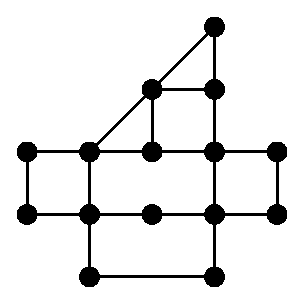
\includegraphics{euler-tour}

\caption{A possible floor plan for a museum. Can you find a walk that
  traverses every edge exactly once?}

\label{fig:5BC}

\end{figure}

The entire field of graph theory began when Euler asked whether the
seven bridges of K\"onigsberg could all be traversed exactly
once---essentially the same question we asked about the Museum of Fine
Arts.  In his honor, an \term{Euler walk} is a defined to be a walk
that traverses every edge in a graph exactly once.  Similarly, an
\term{Euler tour} is an Euler walk that starts and finishes at the
same vertex.  Graphs with Euler tours and Euler walks both have simple
characterizations.
\begin{theorem}\label{thm:euler-tour}
A connected graph has an Euler tour if and only if every vertex has
even degree.
\end{theorem}

\begin{proof}
  We first show that if a graph has an Euler tour, then every vertex has
  even degree.  Assume that a graph $G$ has an Euler tour $v_0$, $v_1$,
  \dots, $v_k$ where $v_k = v_0$.  Since every edge is traversed once in
  the tour, $k = \card{\edges{G}}$ and the degree of a node~$u$ in~$G$ is
  twice the number of times that node~$u$ appears in the sequence $v_0$,
  $v_1$, \dots, $v_{k-1}$.  We multiply by two since if $u = v_i$ for
  some~$i$ where $0 < i < k$, then both $\edge{v_{i - 1}}{v_i}$ and
  $\edge{v_i}{v_{i + 1}}$ are edges incident to~$u$ in~$G$.  If $u = v_0 =
  v_k$, then both $\edge{v_{k - 1}}{v_k}$ and $\edge{v_0}{v_1}$ are edges
  incident to~$u$ in~$G$.  Hence, the degree of every node is even.

We next show that if the degree of every node is even in a graph
$G$, then there is an Euler tour.  Let
\[
W \eqdef v_0, v_1, \dots, v_k
\]
be the longest walk in~$G$ that traverses \emph{no edge more than
  once}.\footnote{Did you notice that we are using a variation of the Well
  Ordering Principle here when we implicitly assume that a longest walk
  exists?  This is ok since the length of a walk where no edge is used
  more than once is at most~$\card{E}$.}  $W$ must traverse every edge
incident to~$v_k$; otherwise the walk could be extended and $W$ would not
be the longest walk that traverses all edges at most once.  Moreover, it
must be that $v_k = v_0$ and that $W$ is a closed walk, since otherwise
$v_k$ would have odd degree in~$W$, and hence in~$G$, which is not
possible by assumption.

We conclude the argument with a proof by contradiction.  Suppose that
$W$ is not an Euler tour.  Because $G$ is a connected graph, we can
find an edge not in $W$ but incident to some vertex in $W$.  Call this
edge $\edge{u}{v_i}$.  But then we can construct a walk $W'$ that is
longer than~$W$ but that still uses no edge more than once:
\begin{equation*}
    W' ::= u, v_i, v_{i + 1}, \dots, v_k, v_1, v_2, \dots, v_i
\end{equation*}
%
This contradicts the definition of $W$, so $W$ must be an
Euler tour after all.
\end{proof}

It is not difficult to extend Theorem~\ref{thm:euler-tour} to prove that a
connected graph~$G$ has an Euler walk if and only if precisely 0 or~2
nodes in~$G$ have odd degree.  Hence, we can conclude that the graph
shown in Figure~\ref{fig:5BC} has an Euler walk but not an Euler tour
since the graph has precisely two nodes with odd degree.

Although the proof of Theorem~\ref{thm:euler-tour} does not explicitly
define a method for finding an Euler tour when one exists, it is not
hard to modify the proof to produce such a method.  The idea is to
grow a tour by continually splicing in closed walks until all the
edges are consumed.

\subsection{Hamiltonian Cycles}

Hamiltonian cycles are the unruly cousins of Euler tours.

\begin{definition}\label{def:hamiltonian-cycle}
A \emph{Hamiltonian cycle} in a graph~$G$ is a cycle that visits every
\emph{node} in~$G$ exactly once.  Similarly, a \emph{Hamiltonian} path
is a path in~$G$ that visits every node exactly once.
\end{definition}

Although Hamiltonian cycles sound similar to Euler tours---one visits
every node once while the other visits every edge once---finding a
Hamiltonian cycle can be a lot harder than finding an Euler tour.  The
same is true for Hamiltonian paths.  This is because no one has
discovered a simple characterization of all graphs with a Hamiltonian
cycle.  In fact, determining whether a graph has a Hamiltonian cycle
is the same category of problem as the SAT problem of
Section~\ref{SAT_sec} and the coloring problem in
Section~\ref{sec:coloring}: you get a million dollars for finding an
efficient way to determine when a graph has a Hamiltonian cycle---or
proving that no procedure works efficiently on all graphs.

\subsection{The Traveling Salesperson Problem}

As if the problem of finding a Hamiltonian cycle is not hard enough,
when the graph is weighted, we often want to find a Hamiltonian cycle
that has least possible weight.  This is a very famous optimization
problem known as the Traveling Salesperson Problem.

\begin{definition}
Given a weighted graph~$G$, the \emph{weight} of a cycle in~$G$ is
defined as the sum of the weights of the edges in the cycle.
\end{definition}

For example, consider the graph shown in Figure~\ref{fig:5AL} and
suppose that you would like to visit every node once and finish at the
node where you started.  Can you find  way to do this by traversing a
cycle with weight~15?

\begin{figure}

\redrawn

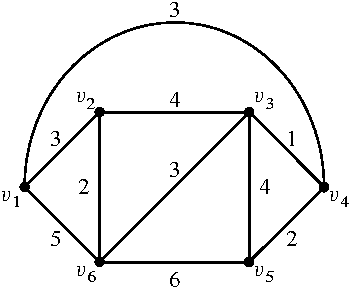
\includegraphics{Fig_5AL}

\caption{A weighted graph.  Can you find a cycle with weight~15 that
  visits every node exactly once?}

\label{fig:5AL}
\end{figure}

Needless to say, if you can figure out a fast procedure that finds the
optimal cycle for the traveling salesperson, let us know so that we
can win a million dollars.

\begin{problems}
\examproblems
\pinput{FP_bipartite_matching_sex}

\homeworkproblems
\pinput{PS_no_odd_length_closed_walks}
\end{problems}

\section{Trees}\label{trees-sec}

As we have just seen, finding good cycles in a graph can be trickier
than you might first think.  But what if a graph has no cycles at all?
Sounds pretty dull.  But graphs without cycles (called \emph{acyclic
  graphs}) are probably the most important graphs of all when it comes
to computer science.

\subsection{Definitions}

\begin{definition}\label{def:tree}
A connected acyclic graph is called a \emph{tree}.
\end{definition}

For example, Figure~\ref{fig:5H} shows an example of a 9-node tree.

\begin{figure}

\redrawn

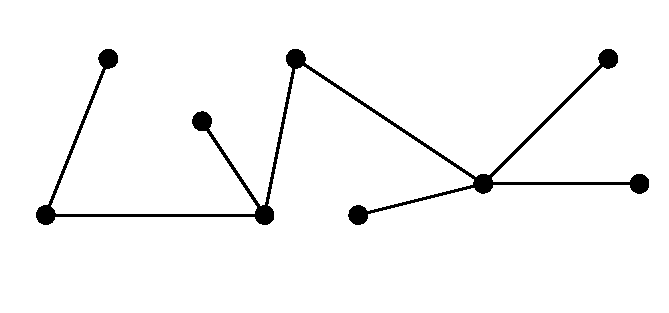
\includegraphics{tree-example}

\caption{A 9-node tree.}
\label{fig:5H}
\end{figure}

The graph shown in Figure~\ref{fig:5I} is not a tree since it is not
connected, but it is a forest.  That's because, of course, it consists
of a collection of trees.

\begin{definition}\label{def:forest}
If every connected component of a graph~$G$ is a tree, then $G$ is a
\emph{forest}.
\end{definition}

\begin{figure}

\redrawn

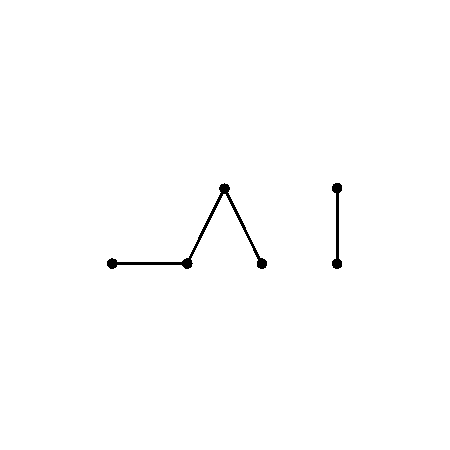
\includegraphics{Fig_5I}

\caption{A 6-node forest consisting of 2 component trees.  Note that
  this 6-node graph is not itself a tree since it is not connected.}
\label{fig:5I}
\end{figure}

One of the first things you will notice about trees is that they tend
to have a lot of nodes with degree one.  Such nodes are called
\emph{leaves}.

\begin{definition}
A \emph{leaf} is a node with degree~1 in a tree (or forest).
\end{definition}

For example, the tree in Figure~\ref{fig:5H} has 5 leaves and the
forest in Figure~\ref{fig:5I} has 4 leaves.

Trees are a fundamental data structure in computer science.  For
example, information is often stored in tree-like data structures and
the execution of many recursive programs can be modeled as the
traversal of a tree.  In such cases, it is often useful to draw the
tree in a leveled fashion where the node in the top level is
identified as the \emph{root}, and where every edge joins a
\emph{parent} to a \emph{child}.  For example, we have redrawn the
tree from Figure~\ref{fig:5H} in this fashion in Figure~\ref{fig:5JJ}.
In this example, node~$d$ is a child of node~$e$ and a parents of
nodes $b$ and~$c$.

\begin{figure}

\redrawn

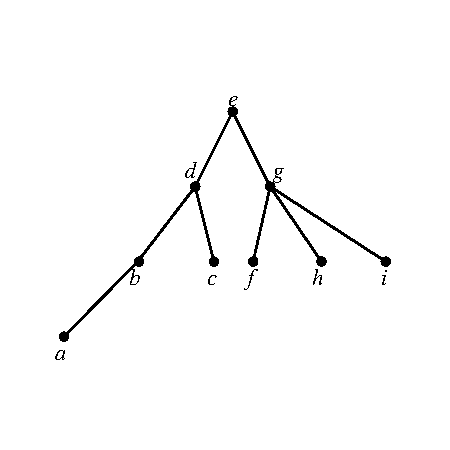
\includegraphics{Fig_5JJ}

\caption{The tree from Figure~\ref{fig:5H} redrawn in a leveled
  fashion, with node~$E$ as the root.}

\label{fig:5JJ}
\end{figure}

In the special case of \emph{ordered binary trees}, every node is the
parent of at most 2 children and the children are labeled as being a
left-child or a right-child.

\subsection{Properties}

Trees have many unique properties.  We have listed some of them in the
following theorem.

\begin{theorem}\label{th:treeprops}
Every tree has the following properties:

\begin{enumerate}

\item Any connected subgraph is a tree.\label{asub}

\item There is a unique simple path between every pair of vertices.

\item Adding an edge between nonadjacent nodes in a tree creates a
  graph with a cycle.

\item Removing any edge disconnects the graph.

\item If the tree has at least two vertices, then it has at least two
  leaves.

\item The number of vertices in a tree is one larger than the number
  of edges.

\end{enumerate}
\end{theorem}

\begin{proof}
\begin{enumerate}

\item A cycle in a subgraph is also a cycle in the whole graph, so any
  subgraph of an acyclic graph must also be acyclic.  If the subgraph
  is also connected, then by definition, it is a tree.

\item Since a tree is connected, there is at least one path between
  every pair of vertices.  Suppose for the purposes of contradiction,
  that there are two different paths between some pair of vertices
  $u$ and~$v$.  Beginning at $u$, let $x$ be the first vertex where
  the paths diverge, and let $y$ be the next vertex they share.  (For
  example, see Figure~\ref{fig:5L}.)  Then there are two paths from
  $x$ to~$y$ with no common edges, which defines a cycle.  This is a
  contradiction, since trees are acyclic.  Therefore, there is
  exactly one path between every pair of vertices.

\begin{figure}

\redrawn

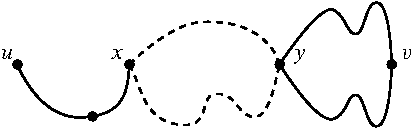
\includegraphics{unique-path}

\caption{If there are two paths between $u$ and~$v$, the graph must
  contain a cycle.}

\label{fig:5L}
\end{figure}

\item An additional edge $\edge{u}{v}$ together with the unique path
  between $u$ and $v$ forms a cycle.

\item Suppose that we remove edge $\edge{u}{v}$.  Since the tree
  contained a unique path between $u$ and $v$, that path must have
  been $\edge{u}{v}$.  Therefore, when that edge is removed, no path
  remains, and so the graph is not connected.

\item Let $v_1, \dots, v_m$ be the sequence of vertices on a longest
  path in the tree.  Then $m \geq 2$, since a tree with two vertices
  must contain at least one edge.  There cannot be an edge
  $\edge{v_1}{v_i}$ for $2 < i \leq m$; otherwise, vertices $v_1,
  \dots, v_i$ would from a cycle.  Furthermore, there cannot be
  an edge $\edge{u}{v_1}$ where $u$ is not on the path; otherwise, we
  could make the path longer.  Therefore, the only edge incident to
  $v_1$ is $\edge{v_1}{v_2}$, which means that $v_1$ is a leaf.  By a
  symmetric argument, $v_m$ is a second leaf.

\item We use induction on the proposition $P(n) \eqdef {}$ there are
  $n - 1$ edges in any $n$-vertex tree.

\inductioncase{Base Case} ($n = 1$): $P(1)$ is true since a tree with
1 node has 0 edges and $1 - 1 = 0$.

\inductioncase{Inductive step}: Now suppose that $P(n)$ is true and
consider an $(n+1)$-vertex tree, $T$.  Let $v$ be a leaf of the tree.
You can verify that deleting a vertex of degree 1 (and its incident
edge) from any connected graph leaves a connected subgraph.  So by
part~\ref{asub} of Theorem~\ref{th:treeprops}, deleting $v$ and its
incident edge gives a smaller tree, and this smaller tree $n - 1$
edges by induction.  If we re-attach the vertex, $v$, and its incident
edge, we find that $T$ has $ = (n + 1) - 1$ edges.  Hence, $P(n + 1)$
is true, and the induction proof is complete.  \qedhere

\end{enumerate}

\end{proof}

Various subsets of properties in Theorem~\ref{th:treeprops} provide
alternative characterizations of trees, though we won't prove this.
For example, a \emph{connected} graph with a number of vertices one
larger than the number of edges is necessarily a tree.  Also, a graph
with unique paths between every pair of vertices is necessarily a
tree.

\subsection{Spanning Trees}

Trees are everywhere.  In fact, every connected graph contains a
subgraph that is a tree with the same vertices as the graph.  This is
a called a \term{spanning tree} for the graph.  For example,
Figure~\ref{fig:5LL} is a connected graph with a spanning tree
highlighted.

\begin{figure}

\redrawn

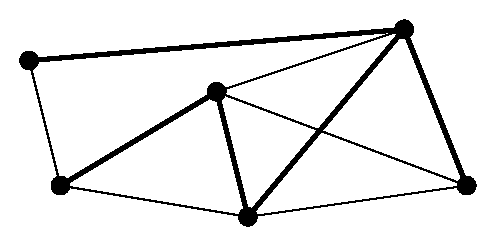
\includegraphics{spanning-tree}

\caption{A graph where the edges of a spanning tree have been
  thickened.}

\label{fig:5LL}

\end{figure}

\begin{theorem}
Every connected graph contains a spanning tree.
\end{theorem}

\begin{proof}
By contradiction.  Assume there is some connected graph~$G$ that has
no spanning tree and let $T$ be a connected subgraph of $G$, with the
same vertices as $G$, and with the smallest number of edges possible
for such a subgraph.  By the assumption, $T$ is not a spanning tree
and so it contains some cycle:
\[
\edge{v_0}{v_1}, \edge{v_1}{v_2}, \dots, \edge{v_k}{v_0}
\]
Suppose that we remove the last edge, $\edge{v_k}{v_0}$.  If a pair
of vertices $x$ and $y$ was joined by a path not containing
$\edge{v_k}{v_0}$, then they remain joined by that path.  On the
other hand, if $x$ and $y$ were joined by a path containing
$\edge{v_k}{v_0}$, then they remain joined by a wallk containing the
remainder of the cycle.  By Lemma~\ref{simplepath}, they must also
then be joined by a path.  So all the vertices of $G$ are still
connected after we remove an edge from $T$.  This is a contradiction,
since $T$ was defined to be a minimum size connected subgraph with
all the vertices of~$G$.  So the theorem must be true.
\end{proof}

\subsection{Minimum Weight Spanning Trees}

Spanning trees are interesting because they connect all the nodes of a
graph using the smallest possible number of edges.  For example the
spanning tree for the 6-node graph shown in Figure~\ref{fig:5LL} has 5
edges.

Spanning trees are very useful in practice, but in the real world, not
all spanning trees are equally desirable.  That's because, in
practice, there are often costs associated with the edges of the graph.

For example, suppose the nodes of a graph represent buildings or towns
and edges represent connections between buildings or towns.  The cost
to actually make a connection may vary a lot from one pair of
buildings or towns to another.  The cost might depend on distance or
topography.  For example, the cost to connect LA to~NY might be much
higher than that to connect NY to Boston.  Or the cost of a pipe
through Manhattan might be more than the cost of a pipe through a
cornfield.

In any case, we typically represent the cost to connect pairs of nodes
with a weighted edge, where the weight of the edge is its cost.  The
weight of a spanning tree is then just the sum of the weights of the
edges in the tree.  For example, the weight of the spanning tree shown
in Figure~\ref{fig:5KA} is~19.

\begin{figure}

\subfloat[]{%
    \redrawn
    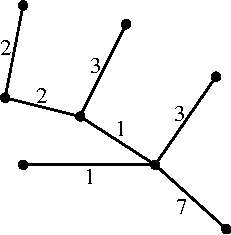
\includegraphics{Fig_5KA-a}
}
%
\qquad
%
\subfloat[]{%
    \redrawn
    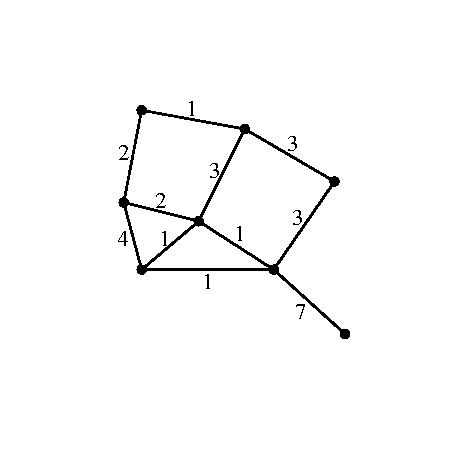
\includegraphics{Fig_5KA-b}
}

\caption{A spanning tree (a) with weight 19 for a graph~(b).}

\label{fig:5KA}

\end{figure}

The goal, of course, is to find the spanning tree with minimum weight,
called the min-weight spanning tree (MST for short).

\begin{definition}
The \emph{min-weight spanning tree} \textup(MST\textup) of an
edge-weighted graph~$G$ is the spanning tree of~$G$ with the smallest
possible sum of edge weights.
\end{definition}

Is the spanning tree shown in Figure~\ref{fig:5KA}(a) an MST of the
weighted graph shown in Figure~\ref{fig:5KA}(b)?  Actually, it is not,
since the tree shown in Figure~\ref{fig:5KB} is also a spanning tree
of the graph shown in Figure~\ref{fig:5KA}(b), and this spanning tree
has weight~17.

\begin{figure}

\redrawn

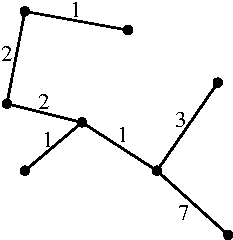
\includegraphics{Fig_5KB}

\caption{An MST with weight~17 for the graph in
  Figure~\ref{fig:5KA}(b).}
\label{fig:5KB}

\end{figure}

What about the tree shown in Figure~\ref{fig:5KB}?  Is it an MST?  It
seems to be, but how do we prove it?  In general, how do we find an
MST\@?  We could, of course, enumerate all trees, but this could take
forever for very large graphs.

\begin{staffnotes}no need or point that I see to having both
  algorithms in the text.  Put one of them in a problem. --ARM 7/4/10.
\end{staffnotes}
Here are two possible algorithms:

\begin{algorithm}\label{alg:MST1}
  Grow a tree one edge at a time by adding the minimum weight edge
  possible to the tree, making sure that you have a tree at each
  step.
\end{algorithm}

\begin{algorithm}\label{alg:MST2}
Grow a subgraph one edge at a time by adding the minimum-weight edge
possible to the subgraph, making sure that you have an acyclic
subgraph at each step.
\end{algorithm}

For example, in the weighted graph we have been considering, we might
run Algorithm~\ref{alg:MST1} as follows.  We would start by choosing
one of the weight~1 edges, since this is the smallest weight in the
graph.  Suppose we chose the weight~1 edge on the bottom of the
triangle of weight~1 edges in our graph.  This edge is incident to two
weight~1 edges, a weight~4 edge, a weight~7 edge, and a weight~3
edge.  We would then choose the incident edge of minimum weight.  In
this case, one of the two weight~1 edges.  At this point, we cannot
choose the third weight~1 edge since this would form a cycle, but we
can continue by choosing a weight~2 edge.  We might end up with the
spanning tree shown in Figure~\ref{fig:5KC}, which has weight~17, the
smallest we've seen so far.

\begin{figure}

\redrawn

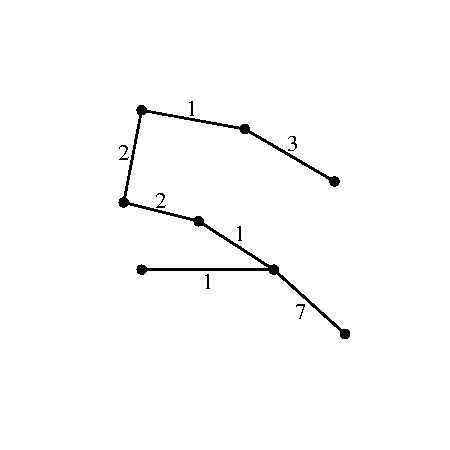
\includegraphics{Fig_5KC}

\caption{A spanning tree found by Algorithm~\ref{alg:MST1}.}

\label{fig:5KC}

\end{figure}

Now suppose we instead ran Algorithm~\ref{alg:MST2} on our graph.  We
might again choose the weight~1 edge on the bottom of the triangle of
weight~1 edges in our graph.  Now, instead of choosing one of the
weight~1 edges it touches, we might choose the weight~1 edge on the
top of the graph.  Note that this edge still has minimum weight, and
does not cause us to form a cycle, so Algorithm~\ref{alg:MST2} can
choose it.  We would then choose one of the remaining weight~1 edges.
Note that neither causes us to form a cycle.  Continuing the
algorithm, we may end up with the same spanning tree in
Figure~\ref{fig:5KC}, though this need not always be the case.

It turns out that both algorithms work, but they might end up with
different MSTs.  The MST is not necessarily unique---indeed, if all
edges of an $n$-node graph have the same weight (${}=1$), then all
spanning trees have weight~$n - 1$.

These are examples of greedy approaches to optimization.  Sometimes it
works and sometimes it doesn't.  The good news is that it works to
find the MST\@.  In fact, both variations work.  It's a little easier
to prove it for Algorithm~\ref{alg:MST2}, so we'll do that one here.

\begin{theorem}\label{thm:MST2}
For any connected, weighted graph~$G$, Algorithm~\ref{alg:MST2}
produces an MST for~$G$.
\end{theorem}

\begin{proof}
The proof is a bit tricky.  We need to show the algorithm terminates,
\ie that if we have selected fewer than $n - 1$ edges, then we can
always find an edge to add that does not create a cycle.  We also need
to show the algorithm creates a tree of minimum weight.

The key to doing all of this is to show that the algorithm never gets
stuck or goes in a bad direction by adding an edge that will keep us
from ultimately producing an MST\@.  The natural way to prove this is
to show that the set of edges selected at any point is contained in
some MST---\ie we can always get to where we need to be.  We'll state
this as a lemma.

\begin{lemma}\label{lemma:MST2}
  For any $m \ge 0$, let $S$ consist of the first $m$ edges selected by
  Algorithm~\ref{alg:MST2}.  Then there exists some MST~$T$ for~$G$ such
  that $S \subseteq \edges{T}$, that is, the set of edges that we are
  growing is always contained in some MST\@.
\end{lemma}

We'll prove this momentarily, but first let's see why it helps prove the
theorem.  Assume the lemma is true.  Then how do we know
Algorithm~\ref{alg:MST2} can always find an edge to add without creating a
cycle?  Well, as long as there are fewer than $n - 1$ edges picked, there
exists some edge in $\edges{T} - S$ and so there is an edge that we can
add to~$S$ without forming a cycle.  Next, how do we know that we get an
MST at the end?  Well, once $m = n - 1$, we know that $S$ is an MST\@.

Ok, so the theorem is an easy corollary of the lemma.  To prove the
lemma, we'll use induction on the number of edges chosen by the
algorithm so far.  This is very typical in proving that an algorithm
preserves some kind of invariant condition---induct on the number of
steps taken, \ie the number of edges added.

Our inductive hypothesis $P(m)$ is the following: for any $G$ and any
set~$S$ of $m$ edges initially selected by Algorithm~\ref{alg:MST2},
there exists an MST $T = (V, E)$ of~$G$ such that $S \subseteq E$.

For the base case, we need to show $P(0)$.  In this case, $S =
\emptyset$, so $S \subseteq E$ trivially holds for any MST $T = (V,
E)$.

For the inductive step, we assume $P(m)$ holds and show that it
implies $P(m + 1)$.  Let $e$ denote the $(m+1)$st edge selected by
Algorithm~\ref{alg:MST2}, and let $S$ denote the first $m$ edges
selected by Algorithm~\ref{alg:MST2}.  Let $T^* = (V^*, E^*)$ be the
MST such that $S \subseteq E^*$, which exists by the inductive
hypothesis.  There are now two cases:
\begin{description}

\item[Case 1:]
$e \in E^*$, in which case $S \union \{e\} \subseteq E^*$, and thus
  $P(m+1)$ holds.

\item[Case 2:]
$e \notin E^*$, as illustrated in Figure~\ref{fig:5KD}.  Now we need
  to find a different MST that contains $S$ and~$e$.

\begin{figure}

\redrawn

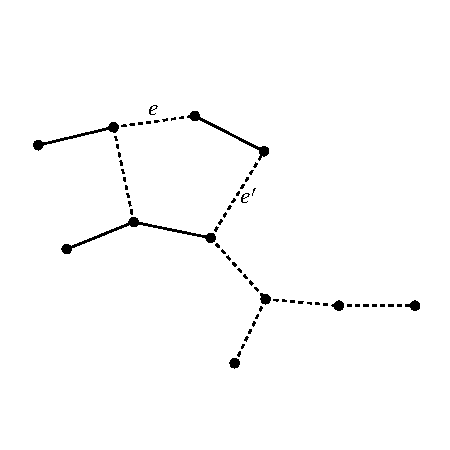
\includegraphics{Fig_5KD}

\caption{The graph formed by adding $e$ to $T^*$.  Edges of~$S$ are
  denoted with solid lines and edges of $E^* - S$ are denoted with
  dashed lines.}

\label{fig:5KD}
\end{figure}

\end{description}

What happens when we add $e$ to~$T^*$?  Since $T^*$ is a tree, we get
a cycle.  (Here we used part~3 of Theorem~\ref{th:treeprops}.)
Moreover, the cycle cannot only contains edges in~$S$, since $e$ was
chosen so that together with the edges in~$S$, it does not form a
cycle.  This implies that $\{e\} \union T^*$ contains a cycle that
contains an edge $e'$ of $E^* - S$.  For example, such an $e'$ is
shown in Figure~\ref{fig:5KD}.

Note that the weight of~$e$ is at most that of~$e'$.  This is because
Algorithm~\ref{alg:MST2} picks the minimum weight edge that does not
make a cycle with~$S$.  Since $e' \in T^*$, \ $e'$ cannot make a cycle
with~$S$, and if the weight of~$e$ were greater than the weight
of~$e'$, Algorithm!\ref{alg:MST2} would no have selected~$e$ ahead
of~$e'$.

Okay, we're almost done.  Now we'll make an MST that contains $S
\union \{e\}$.  Let $T^{**} = (V, E^{**})$ where $E^{**} = (E^* -
\{e'\}) \union \{e\}$, that is, we swap $e$ and~$e'$ in~$T^*$.

\begin{claim}\label{claim:MST2}
$T^{**}$ is an MST.
\end{claim}

\begin{proof}[Proof of claim]
We first show that $T^{**}$ is a spanning tree.  
$T^{**}$ is acyclic
because it was produced by removing an edge from the only cycle in
$T^{*} \union \{e\}$.
$T^{**}$ is connected
since the edge we deleted from $T^* \union \{e\}$ was on a cycle.
Since $T^{**}$ contains all the nodes of~$G$, it must be a spanning
tree for~$G$.

Now let's look at the weight of~$T^{**}$.  Well, since the weight
of~$e$ was at most that of~$e'$, the weight of~$T^{**}$ is at most
that of~$T^*$, and thus $T^{**}$ is an MST for~$G$.
\end{proof}

Since $S \union \{e\} \subseteq E^{**}$, $P(m + 1)$ holds.  Thus, 
Algorithm~\ref{alg:MST2} must eventually produce an MST\@.  This will
happens when it adds $n - 1$ edges to the subgraph it builds.
\end{proof}

So now we know for sure that the MST for our example graph has
weight~17 since it was produced by Algorithm~\ref{alg:MST2}.  And we
have a fast algorithm for finding a minimum-weight spanning tree for
any graph.

%% Trees Problems %%%%%%%%%%%%%%%%%%%%%%%%%%%%%%%%%%%%%%%%%%%%%%%%%%%%%%%%%%%%%
\begin{problems}
\classproblems
\pinput{CP_graph_edge_mark}
\pinput{CP_spanning_tree_proc}
\pinput{CP_tree_characterizations}
%\pinput{CP_23_high_priority_servers}

\homeworkproblems
\pinput{PS_average_degree_of_tree_and_simple_path}
% S09.cp6t.2
% S09.cp6t.3
\end{problems}


%% Coloring  Problems %%%%%%%%%%%%%%%%%%%%%%%%%%%%%%%%%%%%%%%%%%%%%%%%%%%
\begin{problems}
\classproblems
\pinput{CP_chromatic_number}

% S09.cp6r.1
% S09.cp6r.2

\homeworkproblems
\pinput{PS_TA_recitation_graph_coloring}
\pinput{PS_graph_colorable}
%\pinput{PS_simple_triangle_free_graph_coloring}

\examproblems
\pinput{FP_coloring_false_proof}

\end{problems}

%% Bipartite Matchings Problems %%%%%%%%%%%%%%%%%%%%%%%%%%%%%%%%%%%%%%%%%%%%%%%
% S09.cp6r.3
% S09.cp6r.4

\begin{problems}
\classproblems
\pinput{CP_student_clubs}
\pinput{CP_latin_squares}

\examproblems
\pinput{MQ_bipartite-matching_recitations}

\homeworkproblems
\pinput{PS_cards_in_4_rows_13_columns}
\pinput{PS_bipartite_matching_virtues}
\end{problems}

\section{Planar Graphs}\label{planar_graphs_sec}

\subsection{Drawing Graphs in the Plane}

Suppose there are three dogs and three houses, as shown in
Figure~\ref{fig:5DP}.  Can you find a route from each dog to each
house such that no route crosses any other route?

\begin{figure}

\redrawn

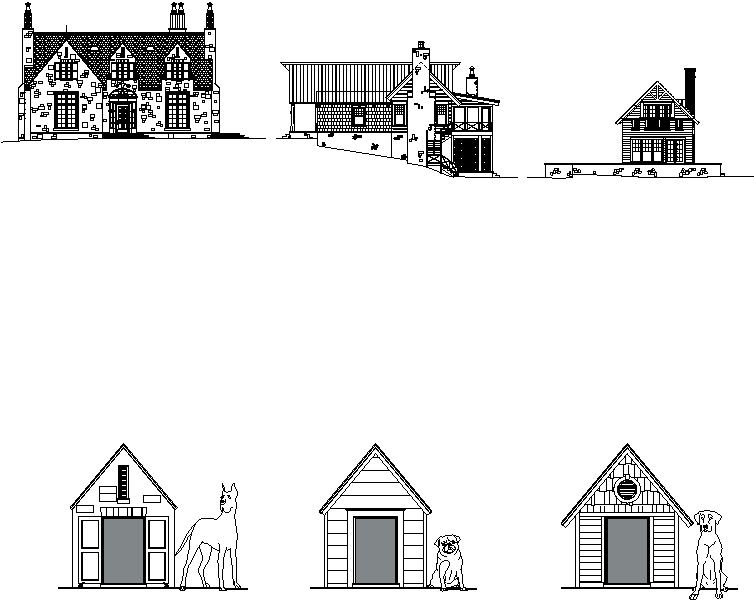
\includegraphics{dog-houses}

\caption{Three dogs and three houses.  Is there a route from each dog
  to each house so that no pair of the 9 routes cross each other?}
\label{fig:5DP}
\end{figure}

For example, Figure~\ref{fig:5DC} \begin{editingnotes}
new figure needed
\end{editingnotes} shows how to route the first two dogs to all threes
houses and the third dog to two of the houses, all without any crossings.
But in this figure there is no way left to route the third dog to the last
house without crossing one of the other routes.  Is there a better routing
that does the job?

A similar question comes up about a little-known animal called a
\emph{quadrapus} that looks like an octopus with four stretchy arms
instead of eight.  If five quadrapi are resting on the sea floor, as shown
in Figure~\ref{fig:5DA}, can each quadrapus simultaneously shake hands
with every other in such a way that no arms cross?

\begin{figure}

%\mfigure{!}{2in}{quadrapi}

\setlength{\unitlength}{2000sp}%{3947sp}%
%
\begingroup\makeatletter\ifx\SetFigFont\undefined%
\gdef\SetFigFont#1#2#3#4#5{%
  \reset@font\fontsize{#1}{#2pt}%
  \fontfamily{#3}\fontseries{#4}\fontshape{#5}%
  \selectfont}%
\fi\endgroup%
\begin{picture}(11049,5049)(589,-5248)
{\color[rgb]{0,0,0}%\thinlines
\put(4688,-1673){\oval(524,524)}
}%
{\color[rgb]{0,0,0}\put(1913,-2948){\oval(524,524)}
}%
{\color[rgb]{0,0,0}\put(4538,-3923){\oval(524,524)}
}%
{\color[rgb]{0,0,0}\put(7838,-3098){\oval(524,524)}
}%
{\color[rgb]{0,0,0}\put(9713,-1748){\oval(524,524)}
}%
{\color[rgb]{0,0,0}\put(4426,-1636){\line(-1, 0){900}}
\multiput(3526,-1636)(-2.67857,-8.03571){57}{\makebox(1.6667,11.6667){\SetFigFont{5}{6}{\rmdefault}{\mddefault}{\updefault}.}}
\put(3376,-2086){\line(-1, 0){750}}
}%
{\color[rgb]{0,0,0}\put(4951,-1711){\line( 5,-3){893.382}}
\put(5851,-2236){\line( 5, 6){442.623}}
\put(6301,-1711){\line( 2,-3){300}}
}%
{\color[rgb]{0,0,0}\multiput(1876,-2686)(1.37838,8.27027){101}{\makebox(1.6667,11.6667){\SetFigFont{5}{6}{\rmdefault}{\mddefault}{\updefault}.}}
\put(2026,-1861){\line( 5, 2){685.345}}
\put(2701,-1561){\line( 0, 1){375}}
}%
{\color[rgb]{0,0,0}\put(2176,-2986){\line( 5, 2){750}}
\put(2926,-2686){\line( 5,-6){510.246}}
\put(3451,-3286){\line( 6, 1){450}}
}%
{\color[rgb]{0,0,0}\put(1951,-3211){\line(-1,-2){300}}
\put(1651,-3811){\line( 5,-6){375}}
\put(2026,-4261){\line( 3, 2){450}}
}%
{\color[rgb]{0,0,0}\put(1651,-2986){\line(-6, 5){612.295}}
\put(1051,-2461){\line(-5,-6){442.623}}
\multiput(601,-2986)(2.02703,-8.10811){75}{\makebox(1.6667,11.6667){\SetFigFont{5}{6}{\rmdefault}{\mddefault}{\updefault}.}}
}%
{\color[rgb]{0,0,0}\multiput(4501,-3661)(1.37838,8.27027){101}{\makebox(1.6667,11.6667){\SetFigFont{5}{6}{\rmdefault}{\mddefault}{\updefault}.}}
\put(4651,-2836){\line( 5, 2){685.345}}
\put(5326,-2536){\line( 0, 1){375}}
}%
{\color[rgb]{0,0,0}\put(4801,-3961){\line( 5, 2){750}}
\put(5551,-3661){\line( 5,-6){510.246}}
\put(6076,-4261){\line( 6, 1){450}}
}%
{\color[rgb]{0,0,0}\put(4576,-4186){\line(-1,-2){300}}
\put(4276,-4786){\line( 5,-6){375}}
\put(4651,-5236){\line( 3, 2){450}}
}%
{\color[rgb]{0,0,0}\put(7576,-3061){\line(-1, 0){900}}
\multiput(6676,-3061)(-2.67857,-8.03571){57}{\makebox(1.6667,11.6667){\SetFigFont{5}{6}{\rmdefault}{\mddefault}{\updefault}.}}
\put(6526,-3511){\line(-1, 0){750}}
}%
{\color[rgb]{0,0,0}\put(7876,-2836){\line(-1, 1){375}}
\put(7501,-2461){\line( 4, 3){600}}
\put(8101,-2011){\line( 0, 1){450}}
}%
{\color[rgb]{0,0,0}\put(8101,-3136){\line( 5,-3){893.382}}
\put(9001,-3661){\line( 5, 6){442.623}}
\put(9451,-3136){\line( 2,-3){300}}
}%
{\color[rgb]{0,0,0}\put(7876,-3361){\line(-2,-5){237.931}}
\put(7651,-3961){\line( 1,-1){600}}
}%
{\color[rgb]{0,0,0}\put(9751,-1486){\line(-1, 1){375}}
\put(9376,-1111){\line( 4, 3){600}}
\put(9976,-661){\line( 0, 1){450}}
}%
{\color[rgb]{0,0,0}\put(9976,-1786){\line( 5,-3){893.382}}
\put(10876,-2311){\line( 5, 6){442.623}}
\put(11326,-1786){\line( 2,-3){300}}
}%
{\color[rgb]{0,0,0}\put(9751,-2011){\line(-2,-5){237.931}}
\put(9526,-2611){\line( 1,-1){600}}
}%
{\color[rgb]{0,0,0}\put(9451,-1711){\line(-5,-1){677.885}}
\put(8776,-1861){\line(-2, 3){692.308}}
\put(8101,-811){\line(-5,-1){1572.115}}
}%
{\color[rgb]{0,0,0}\put(4651,-1936){\line(-1,-4){339.706}}
\put(4276,-3286){\line(-4,-1){1358.823}}
\multiput(2926,-3661)(-1.37838,-8.27027){101}{\makebox(1.6667,11.6667){\SetFigFont{5}{6}{\rmdefault}{\mddefault}{\updefault}.}}
}%
{\color[rgb]{0,0,0}\put(4276,-3886){\line(-3,-2){761.538}}
\multiput(3526,-4411)(2.03287,-8.13149){103}{\makebox(1.6667,11.6667){\SetFigFont{5}{6}{\rmdefault}{\mddefault}{\updefault}.}}
}%
{\color[rgb]{0,0,0}\multiput(4726,-1411)(-1.37387,8.24324){91}{\makebox(1.6667,11.6667){\SetFigFont{5}{6}{\rmdefault}{\mddefault}{\updefault}.}}
\put(4651,-661){\line( 2,-1){1290}}
\put(5926,-1336){\line( 6,-1){1277.027}}
}%
\end{picture}%


\caption{Five quadrapi (4-armed creatures).}

\label{fig:5DA}

\end{figure}

\begin{staffnotes}
rephrased by ARM 7/3/10:
\end{staffnotes}

Both these puzzles can be understood as asking about drawing graphs in the
plane.  Replacing dogs and houses by nodes, the dog house puzzle can be
rephrased as asking whether there is a planar drawing of the graph with
six nodes and edges between each of the first three nodes and each of the
second three nodes.  This graph is called the \term{complete bipartite
  graph}\idx{$K_{3,3}$} and is shown in Figure~\ref{fig:nonplanar}.(a).
\begin{editingnotes}
Insert graphic and fix figure refs.
\end{editingnotes}
The quadrapi puzzle asks whether there is a planar drawing of the \idx{complete graph}
\idx{$K_5$} shown in Figure~\ref{fig:nonplanar}.(b).

\begin{figure}
%\mfigure{!}{1.5in}{nonplanar}
\setlength{\unitlength}{3000sp}%{3947sp}%
%
\begingroup\makeatletter\ifx\SetFigFont\undefined%
\gdef\SetFigFont#1#2#3#4#5{%
  \reset@font\fontsize{#1}{#2pt}%
  \fontfamily{#3}\fontseries{#4}\fontshape{#5}%
  \selectfont}%
\fi\endgroup%
\begin{picture}(7366,2266)(2318,-2244)
{\color[rgb]{0,0,0}%\thinlines
\put(2401,-661){\circle{150}}
}%
{\color[rgb]{0,0,0}\put(4726,-661){\circle{150}}
}%
{\color[rgb]{0,0,0}\put(3601,-661){\circle{150}}
}%
{\color[rgb]{0,0,0}\put(3601,-2161){\circle{150}}
}%
{\color[rgb]{0,0,0}\put(2401,-2161){\circle{150}}
}%
{\color[rgb]{0,0,0}\put(4801,-2161){\circle{150}}
}%
{\color[rgb]{0,0,0}\put(8401,-61){\circle{150}}
}%
{\color[rgb]{0,0,0}\put(7201,-961){\circle{150}}
}%
{\color[rgb]{0,0,0}\put(9601,-961){\circle{150}}
}%
{\color[rgb]{0,0,0}\put(7801,-2161){\circle{150}}
}%
{\color[rgb]{0,0,0}\put(9001,-2161){\circle{150}}
}%
{\color[rgb]{0,0,0}\put(2401,-661){\line( 0,-1){1500}}
\put(2401,-2161){\line( 4, 5){1200}}
\put(3601,-661){\line( 4,-5){1200}}
\put(4801,-2161){\line( 0, 1){1500}}
\put(4726,-661){\line(-3,-4){1125}}
\put(3601,-2161){\line(-4, 5){1200}}
}%
{\color[rgb]{0,0,0}\put(3601,-661){\line( 0,-1){1500}}
}%
{\color[rgb]{0,0,0}\put(2401,-661){\line( 5,-3){2426.471}}
}%
{\color[rgb]{0,0,0}\put(4726,-661){\line(-3,-2){2301.923}}
}%
{\color[rgb]{0,0,0}\put(7201,-961){\line( 1,-2){600}}
\put(7801,-2161){\line( 1, 0){1200}}
\put(9001,-2161){\line( 1, 2){600}}
\put(9601,-961){\line(-4, 3){1200}}
\put(8401,-61){\line(-4,-3){1200}}
\put(7201,-961){\line( 1, 0){2400}}
\put(9601,-961){\line(-3,-2){1800}}
\put(7801,-2161){\line( 1, 4){529.412}}
\put(8401,-61){\line( 1,-4){529.412}}
}%
{\color[rgb]{0,0,0}\put(9001,-2161){\line(-3, 2){1800}}
}%
\end{picture}%

\caption{$K_{3, 3}$ (a) and $K_5$ (b).  Can you redraw these graphs so
that no pairs of edges cross?}
\label{fig:nonplanar}
\end{figure}

In each case, the answer is, ``No---but almost!''  In fact, if you remove
an edge from either of these graphs, then the resulting graph \emph{can}
be redrawn in the plane so that no edges cross.  Figure~\ref{fig:5EF}
already showed how to do this for $K_{3,3}$ with one edge removed, and
Figure~\ref{fig:5DC} 
shows how to do this for $K_5$ with one edge removed.

\begin{figure}

\redrawn

\gnote{Figure DC, p.~495 of ftl-ch5.8.pdf.  Split into two
  subgraphics.}

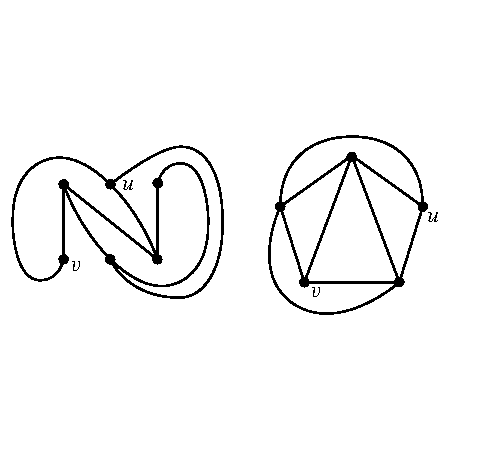
\includegraphics{Fig_5DC}

\caption{Planar drawings of (a) $K_{3, 3} - \edge{u}{v}$, and (b) $K_5
  - \edge{u}{v}$.}
\label{fig:5DC}
\end{figure}

Planar drawings have applications in circuit layout and are helpful in
displaying graphical data such as program flow charts, organizational
charts, and scheduling conflicts.  For these applications, the goal is
to draw the graph in the plane with as few edge crossings as possible.
(See the box on the following page for one such example.)

\begin{figure}
\textbox{\noindent
When wires are arranged on a surface, like a circuit board or microchip,
crossings require troublesome three-dimensional structures.  When Steve
Wozniak designed the disk drive for the early Apple II computer, he
struggled mightily to achieve a nearly planar design:
%
\begin{quotation}
\noindent For two weeks, he worked late each night to make a satisfactory
design.  When he was finished, he found that if he moved a connector he
could cut down on feedthroughs, making the board more reliable.  To make
that move, however, he had to start over in his design.  This time it only
took twenty hours. He then saw another feedthrough that could be
eliminated, and again started over on his design.  ``The final design was
generally recognized by computer engineers as brilliant and was by
engineering aesthetics beautiful.  Woz later said, 'It's something you can
only do if you're the engineer and the PC board layout person yourself.
That was an artistic layout.  The board has virtually no
feedthroughs.'\,''\footnote{From apple2history.org which in turn quotes
\emph{Fire in the Valley} by Freiberger and Swaine.}
\end{quotation}
}
\end{figure}

\subsection{Definitions of Planar Graphs}\label{sec:recdef_planar}

We took the idea of a planar drawing for granted in the previous
section, but if we're going to \emph{prove} things about planar graphs, we
better have precise definitions.

\begin{definition}\label{def:planar_drawing}
A \term{drawing} of a graph assigns to each node a distinct point in
the plane and assigns to each edge a smooth curve in the plane whose
endpoints correspond to the nodes incident to the edge.  The drawing
is \index{planar drawing}\emph{planar} if none of the curves
cross themselves or other curves, namely, the only points that
appear more than once on any of the curves are the node points.  A
graph is \index{planar graph}\emph{planar} when it has a planar
drawing.
\end{definition}

Definition~\ref{def:planar_drawing} is precise but depends on
further concepts: ``smooth planar curves'' and ``points appearing more
than once'' on them.  We haven't defined these concepts---we just
showed the simple picture in Figure~\ref{fig:5DC} and hoped you would
get the idea.

Pictures can be a great way to get a new idea across, but it is generally
not a good idea to use a picture to replace precise mathematics.  Relying
solely on pictures can sometimes lead to disaster---or to false proofs,
anyway.  There is a long history of false proofs about planar graphs based
on misleading pictures.\footnote{The false proof of the
  4-Color Theorem for planar graphs is not the only example.  Mistakes
  creep in with statements like,
\begin{quote}
    As you can see from Figure~ABC, it must be that property~XYZ holds
    for all planar graphs.
\end{quote}}

The bad news is that to prove things about planar graphs using the planar
drawings of Definition~\ref{def:planar_drawing}, we'd have to take a chapter-long
excursion into continuous mathematics just to develop the needed concepts
from plane geometry and topology.
\begin{editingnotes} and this makes
  Definition~\ref{def:planar_drawing} troublesome.
\end{editingnotes}
The good news is that there is another way to define planar graphs that
uses only discrete mathematics.  In particular, we can define planar
graphs as a recursive data type.  In order to understand how it works, we
first need to understand the concept of a \emph{face} in a planar drawing.

\subsubsection{Faces}

In a planar drawing of a graph. the curves corresponding to the edges
divide up the plane into connected regions.  We call these regions the
\term{continuous faces}\footnote{Most texts drop the adjective
  \emph{continuous} from the definition of a face as a connected region.
  We need the adjective to distinguish continuous faces from the
  \emph{discrete} faces we're about to define.}  For example, the drawing
in Figure~\ref{fig:continuous-faces} has four continuous faces.  Face IV,
which extends off to infinity in all directions, is called the
\term{outside face}.

\begin{figure}

\gnote{Fix label of region III.  Fig. 11.1, p. 497, ftl-ch5.8.pdf}

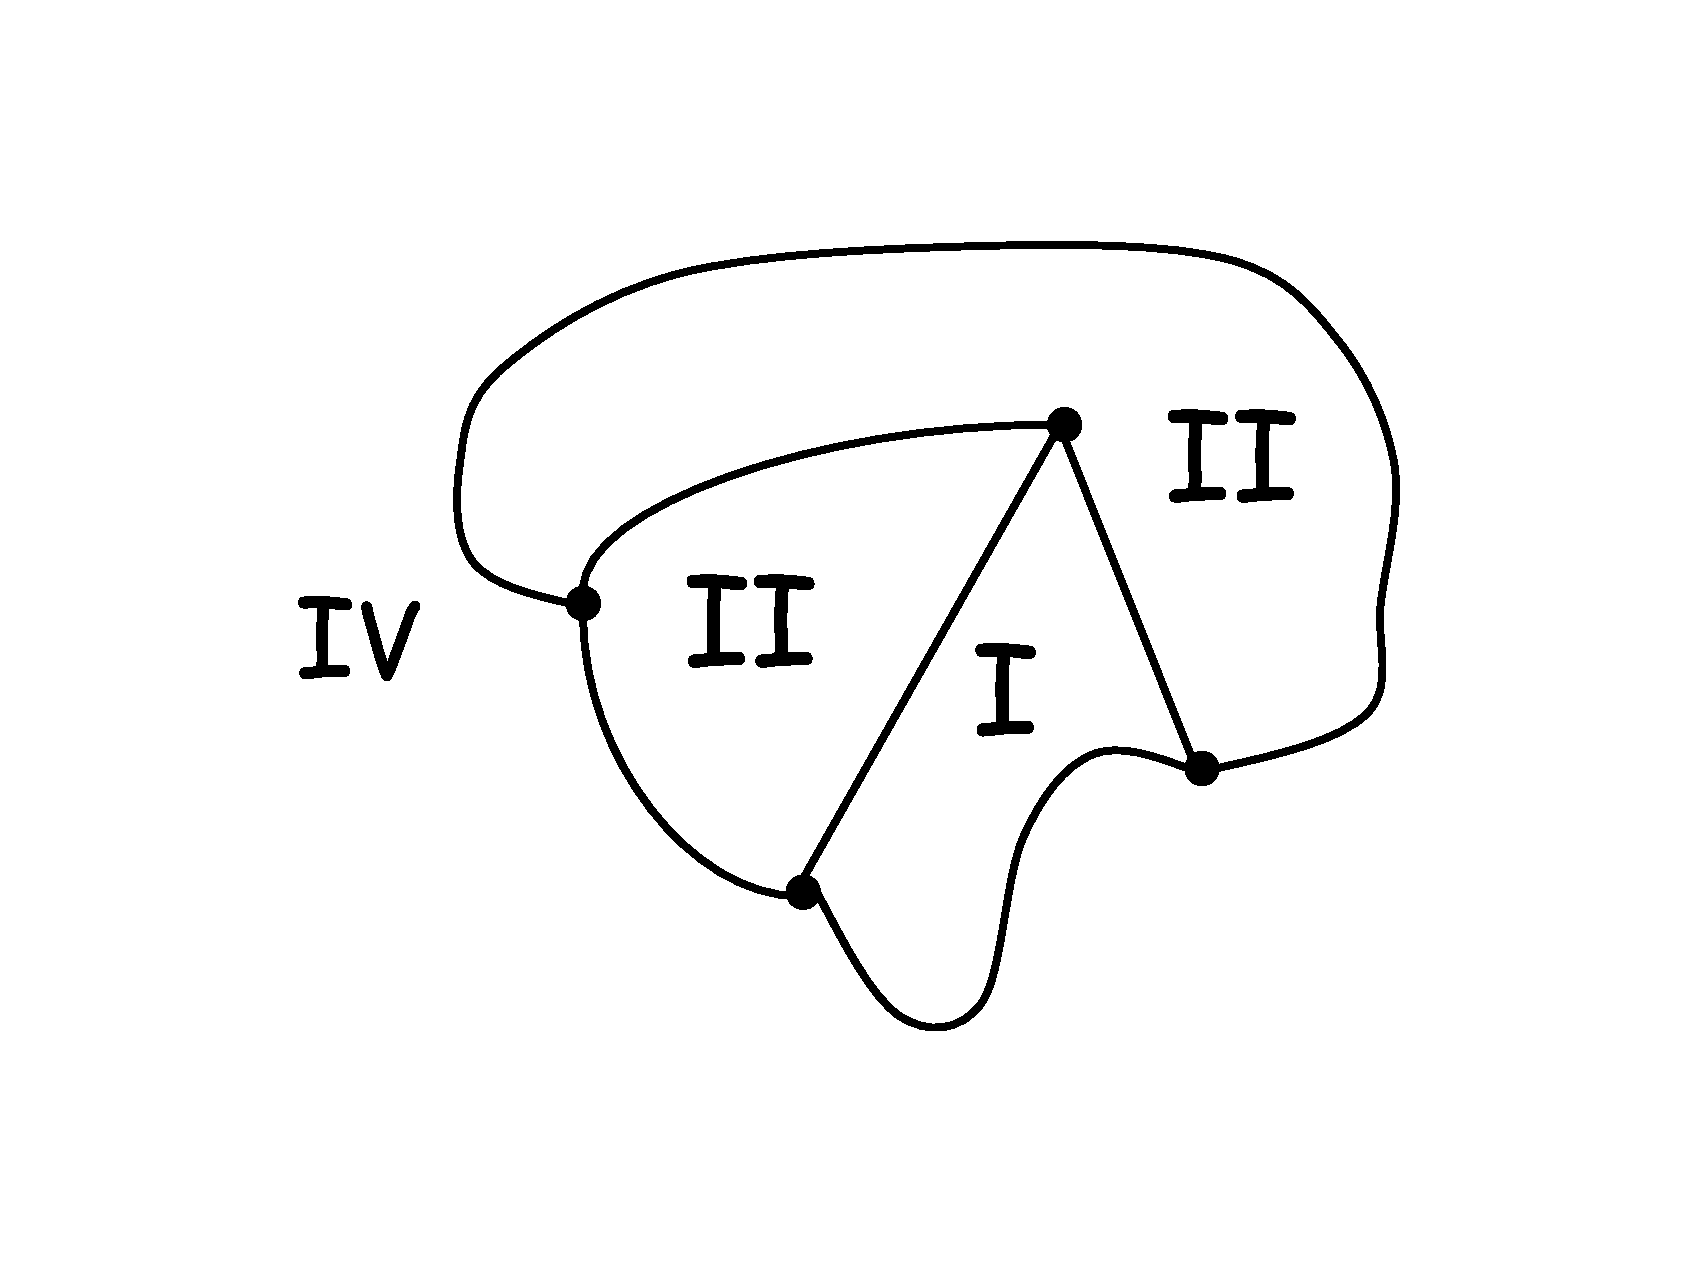
\includegraphics[height=2in]{continuous-faces}

\caption{A planar drawing with four continuous faces.}
\label{fig:continuous-faces}
\end{figure}

The vertices along the boundary of each continuous face in
Figure~\ref{fig:continuous-faces} form a cycle.  For example, labeling the
vertices as in Figure~\ref{fig:continuous-cycles}, the cycles for the face
boundaries are
\begin{equation}\label{eq:5DA}
abca \qquad abda \qquad bcdb \qquad acda.
\end{equation}
These four cycles correspond nicely to the four continuous faces in
Figure~\ref{fig:continuous-cycles}---so nicely, in fact, that we can
identify each of the faces in Figure~\ref{fig:continuous-cycles} by
its cycle.  For example, the cycle $abca$ identifies
face~III\@.  The cycles in list~\ref{eq:5DA} are called the
\emph{discrete faces} of the graph in
Figure~\ref{fig:continuous-cycles}.  We use the term ``discrete''
since cycles in a graph are a discrete data type---as opposed to a
region in the plane, which is a continuous data type.

\begin{figure}

\gnote{Add labels.  Fig. 11.2, p. 499, ftl-ch5.8.pdf}

\includegraphics[height=2in]{continuous-cycles}

\caption{The drawing with labeled vertices.}
\label{fig:continuous-cycles}
\end{figure}

Unfortunately, continuous faces in planar drawings are not always
bounded by cycles in the graph---things can get a little more
complicated.  For example, the planar drawing in
Figure~\ref{fig:bridge} has what we will call a \emph{bridge}, namely,
the edge $\edge{c}{e}$.  The sequence of vertices along the boundary
of the outer region of the drawing is
\[
abcefgecda.
\]
This sequence defines a closed walk, but does not define a cycle since
the walk traverses the bridge $\edge{c}{e}$ twice.

\begin{figure}
\includegraphics[height=2in]{edge-twice-same-face}
\caption{A planar drawing with a \emph{bridge}.}
\label{fig:bridge}
\end{figure}

The planar drawing in Figure~\ref{fig:dongle} illustrates another
complication.  This drawing has what we will call a \emph{dongle},
namely, the nodes $v$, $x$, $y$, and~$w$, and the edges incident to
them.  The sequence of vertices along the boundary
of the inner region is
\[
rstvxyxvwvtur.
\]
This sequence defines a closed walk, but once again does not define a
cycle, because the walk traverses \emph{every} edge of the dongle
twice---once ``coming'' and once ``going.''

\begin{figure}
\includegraphics[height=2in]{dongle-face}
\caption{A planar drawing with a \emph{dongle}.}
\label{fig:dongle}
\end{figure}

It turns out that bridges and dongles are the only complications, at least
for connected graphs.  In particular, every continuous face in a planar
drawing corresponds to a closed walk in the graph.  These closed walks
will be called the \emph{discrete faces} of the drawing, and we'll define
them next.

\subsubsection{A Recursive Definition for Planar Embeddings}

The association between the continuous faces of a planar drawing and
closed walks will allow us to characterize a planar drawing in terms
of the closed walks that bound the continuous faces.  In particular,
it leads us to the discrete data type of \term{planar embeddings}
that we can use in place of continuous planar drawings.  Namely,
we'll define a planar embedding recursively to be the set of
boundary-tracing closed walks that we could get by drawing one edge
after another.

\begin{definition}\label{def:embedding}\label{embeddingdef}
A \term{planar embedding} of a \emph{connected} graph consists of a
nonempty set of closed walks of the graph called the \term{discrete
  faces} of the embedding.  Planar embeddings are defined recursively
as follows:

\inductioncase{Base case}: If $G$ is a graph consisting of a single
vertex, $v$, then a planar embedding of $G$ has one discrete face,
namely, the length zero closed walk, $v$.

\inductioncase{Constructor Case} (split a face): Suppose $G$ is a
connected graph with a planar embedding, and suppose $a$ and $b$ are
distinct, nonadjacent vertices of $G$ that appear on some discrete
face, $\gamma$, of the planar embedding.  That is, $\gamma$ is a
closed walk of the form
\[
a \dots b \cdots a.
\]
Then the graph obtained by adding the edge $\edge{a}{b}$ to the edges of
$G$ has a planar embedding with the same discrete faces as $G$, except
that face $\gamma$ is replaced by the two discrete
faces\footnote{\label{C} There is a minor exception to this definition of
  embedding in the special case when $G$ is a line graph beginning with
  $a$ and ending with $b$.  In this case the cycles into which $\gamma$
  splits are actually the same.  That's because adding edge $\edge{a}{b}$
  creates a cycle that divides the plane into ``inner'' and ``outer''
  continuous faces that are both bordered by this cycle.  In order to
  maintain the correspondence between continuous faces and discrete faces
  in this case, we define the two discrete faces of the embedding to be
  two ``copies'' of this same cycle.}
\[
a\dots ba\quad \text{ and } \quad ab\cdots a,
\]
as illustrated in Figure~\ref{fig:face-splitting}.

\begin{figure}
\includegraphics[height=2.5in]{split-a-face}
\caption{The ``split a face'' case.}
\label{fig:face-splitting}
\end{figure}

\inductioncase{Constructor Case} (add a bridge): Suppose $G$ and~$H$
are connected graphs with planar embeddings and disjoint sets of
vertices.  Let $a$ be a vertex on a discrete face, $\gamma$, in the
embedding of $G$.  That is, $\gamma$ is of the form
\[
a\dots a.
\]
Similarly, let $b$ be a vertex on a discrete face, $\delta$, in the
embedding of $H$.  So $\delta$ is of the form
\[
b\cdots b.
\]
Then the graph obtained by connecting $G$ and $H$ with a new edge,
$\edge{a}{b}$, has a planar embedding whose discrete faces are the union of
the discrete faces of $G$ and $H$, except that faces $\gamma$ and $\delta$
are replaced by one new face
\[
a\dots ab\cdots ba.
\]
This is illustrated in Figure~\ref{fig:add-bridge}, where the faces of
$G$ and $H$ are:
\[
G: \set{ axyza,\; axya,\; ayza }
    \qquad H: \set{ btuvwb,\; btvwb,\; tuvt },
\]
and after adding the bridge $\edge{a}{b}$, there is a
single connected graph with faces
\[
\set{ axyz{\color{blue}ab}tuvw{\color{blue}ba},\;
         axya,\; ayza,\; btvwb,\; tuvt }.
\]

\begin{figure}
\includegraphics[height=3in]{add-bridge}
\caption{The ``add a bridge'' case.}
\label{fig:add-bridge}
\end{figure}

\end{definition}

\subsubsection{Does It Work?}

Yes!  In general, a graph is planar if and only if each of its
connected components has a planar embedding as defined in
Definition~\ref{def:embedding}.  Unfortunately, proving this fact
requires a bunch of mathematics that we don't cover in this
text---stuff like geometry and topology.  Of course, that is why we
went to the trouble of including Definition~\ref{def:embedding}---we
don't want to deal with that stuff in this text and now that we have a
recursive definition for planar graphs, we won't need to.  That's the
good news.

The bad news is that Definition~\ref{def:embedding} looks a lot more
complicated than the intuitively simple notion of a drawing where
edges don't cross.  It seems like it would be easier to stick to the
simple notion and give proofs using pictures.  Perhaps so, but your
proofs are more likely to be complete and correct if you work from the
discrete Definition~\ref{def:embedding} instead of the continuous
Definition~\ref{def:planar_drawing}.

\subsubsection{Where Did the Outer Face Go?}

Every planar drawing has an immediately-recognizable outer face---its
the one that goes to infinity in all directions.  But where is the
outer face in a planar embedding?

There isn't one!  That's because there really isn't any need to
distinguish one.  In fact, a planar embedding could be drawn with any
given face on the outside.  An intuitive explanation of this is to
think of drawing the embedding on a \emph{sphere} instead of the
plane.  Then any face can be made the outside face by ``puncturing''
that face of the sphere, stretching the puncture hole to a circle
around the rest of the faces, and flattening the circular drawing onto
the plane.

So pictures that show different ``outside'' boundaries may actually be
illustrations of the same planar embedding.  For example, the two
embeddings shown in Figure~\ref{fig:5DE} are really the same.

\begin{figure}

\redrawn

\gnote{Confusion: Figure DE, p. 505, ftl-ch5.8.pdf}

\includegraphics{Fig_5DE}

\caption{Two illustrations of the same embedding.}
\label{fig:5DE}
\end{figure}

This is what justifies the ``add bridge'' case in
Definition~\ref{def:embedding}: whatever face is chosen in the
embeddings of each of the disjoint planar graphs, we can draw a
bridge between them without needing to cross any other edges in the
drawing, because we can assume the bridge connects two ``outer''
faces.

\subsection{Euler's Formula}

The value of the recursive definition is that it provides a powerful
technique for proving properties of planar graphs, namely, structural
induction.  For example, we will now use
Definition~\ref{def:embedding} and structural induction to establish
one of the most basic properties of a connected planar graph; namely,
the number of vertices and edges completely determines the number of
faces in every possible planar embedding of the graph.

\begin{theorem}[\idx{Euler's Formula}]\label{thm:eulers_formula}
If a connected graph has a planar embedding, then
\begin{equation*}
    v - e + f = 2
\end{equation*}
where $v$ is the number of vertices, $e$ is the number of edges, and
$f$ is the number of faces.
\end{theorem}

For example, in Figure~\ref{fig:continuous-faces}, $\card{V} = 4$,
$\card{E} = 6$, and $f = 4$.  Sure enough, $4 - 6 + 4 = 2$, as Euler's
Formula claims.

\begin{proof}
The proof is by structural induction on the definition of planar
embeddings.  Let $P(\embed{E})$ be the proposition that $v - e + f = 2$ for an
embedding, $\embed{E}$.

\inductioncase{Base case}: ($\embed{E}$ is the one-vertex planar
embedding).  By definition, $v=1$, $e=0$, and $f=1$, so $P(\embed{E})$
indeed holds.

\inductioncase{Constructor case} (split a face): Suppose $G$ is a
connected graph with a planar embedding, and suppose $a$ and $b$ are
distinct, nonadjacent vertices of $G$ that appear on some discrete
face, $\gamma= a \dots b \cdots a$, of the planar embedding.

Then the graph obtained by adding the edge $\edge{a}{b}$ to the edges of
$G$ has a planar embedding with one more face and one more edge than $G$.
So the quantity $v-e+f$ will remain the same for both graphs, and since by
structural induction this quantity is 2 for $G$'s embedding, it's also 2
for the embedding of $G$ with the added edge.  So $P$ holds for the
constructed embedding.

\inductioncase{Constructor case} (add bridge): Suppose $G$ and $H$ are
connected graphs with planar embeddings and disjoint sets of vertices.
Then connecting these two graphs with a bridge merges the two bridged
faces into a single face, and leaves all other faces unchanged.  So
the bridge operation yields a planar embedding of a connected graph
with $v_G +v_H$ vertices, $e_G + e_H +1$ edges, and $f_G + f_H - 1$
faces.  Since
\begin{align*}
\lefteqn{(v_G +v_H) - (e_G + e_H +1) + (f_G + f_H - 1)} \qquad\\
   & = (v_G  - e_G + f_G) + (v_H  - e_H  + f_H) -2\\
   & = (2)+(2)-2 \qquad \text{(by structural induction hypothesis)}\\
   & = 2,
\end{align*}
$v-e+f$ remains equal to~2 for the constructed embedding.  That is,
$P(e)$ also holds in this case.

This completes the proof of the constructor cases, and the theorem follows
by structural induction.
\end{proof}

\subsection{Bounding the Number of Edges in a Planar Graph}

Like Euler's formula, the following lemmas follow by structural induction
directly from Definition~\ref{def:embedding}.

\begin{lemma}\label{2e}
In a planar embedding of a connected graph, each edge is traversed once by
each of two different faces, or is traversed exactly twice by one face.
\end{lemma}

\begin{lemma}\label{3f}
  In a planar embedding of a connected graph with at least three vertices,
  each face is of length at least three.
\end{lemma}

Combining Lemmas~\ref{2e} and~\ref{3f} with Euler's Formula, we can
now prove that planar graphs have a limited number of edges:

\begin{theorem}\label{th:e3v}
  Suppose a connected planar graph has $v \geq 3$ vertices and $e$
  edges.  Then
\begin{equation}\label{eq:e3v}
    e \leq 3v-6.
\end{equation}
\end{theorem}

\begin{proof}
By definition, a connected graph is planar iff it has a planar embedding.
So suppose a connected graph with $v$ vertices and $e$ edges has a planar
embedding with $f$ faces.  By Lemma~\ref{2e}, every edge is traversed
exactly twice by the face boundaries.  So the sum of the lengths of the
face boundaries is exactly $2e$.  Also by Lemma~\ref{3f}, when $v \geq 3$,
each face boundary is of length at least three, so this sum is at least
$3f$.  This implies that
\begin{equation}\label{e3f}
3f \leq 2e.
\end{equation}
But $f = e-v+2$ by Euler's formula, and substituting into~\eqref{e3f} gives
\begin{align*}
3(e-v+2) & \leq 2e\\
e-3v + 6  & \leq 0\\
e & \leq 3v - 6 \qedhere
\end{align*}
\end{proof}

\subsection{Returning to $K_5$ and $K_{3,3}$}

Finally we have a simple way to answer the quadrapi question at the
begiing of this chapter: the five quadrapi can't all shake hands without
crossing.  The reason is that we know the quadrupi question is the same as
asking whether the complete graph $K_5$ is planar, and 
Theorem~\ref{th:e3v} has the immediate:
\begin{corollary}\label{k5not}
$K_5$ is not planar.
\end{corollary}
\begin{proof}
  $K_5$ is connected and has 5 vertices and 10 edges.  But since $10 > 3
  \cdot 5-6$, $K_5$ does not satisfy the inequality~\eqref{eq:e3v} that
  holds in all planar graphs.
\end{proof}

We can also use Euler's Formula to show that $K_{3, 3}$ is not
planar.  The proof is similar to that of Theorem~\ref{eq:e3v} except that
we use the additional fact that $K_{3, 3}$ is a bipartite graph.

\begin{editingnotes}
\begin{lemma*}\label{lem:5D5}
Every closed walk in a bipartite graph has even length.
\end{lemma*}

\begin{proof}
A bipartite graph $G$ is defined by the property that $\vertices{G}$
are partitioned into two sets $L$ and~$R$ where every edge
connects a node in~$L$ to a node in~$R$.  Hence, any closed walk
in~$G$ must alternate between a node in~$L$ followed by a node
in~$R$.  Since a closed walk ends on the same node it started with, it
must visit nodes in~$L$ equally often as it visits nodes in~$R$.
Hence it must have even length.
\end{proof}

\begin{corollary}\label{cor:5D6}
In a planar embedding of a connected \emph{bipartite} graph with at
least 3 vertices, each face has length at least~4.
\end{corollary}
\begin{proof}
  By Lemma~\ref{3f}, every face has length~3.  Since the graph is
  bipartite and since each face is a closed walk, Lemma~\ref{lem:5D5}
  implies that no face can have length~3.  Hence, every face must have
  length at least~4.
\end{proof}
\end{editingnotes}

\begin{lemma}\label{lem:5D6}
In a planar embedding of a connected \idx{bipartite graph} with at
least 3 vertices, each face has length at least~4.
\end{lemma}

\begin{proof}
  By Lemma~\ref{3f}, every face of a planar embedding of the graph has
  length at least~3.  But a bipartite graph can't have odd length closed
  walks, as was shown in Problem~\ref{PS_no_odd_length_closed_walks}.
  Since the faces of a planar embedding are closed walks, there can't be
  any faces of length 3 in a bipartite embedding.   So every face must have
  length at least~4.
\end{proof}

\begin{theorem}\label{th:e2v}
Suppose a connected bipartite graph with $v \geq 3$ vertices and $e$ edges
is planar.  Then
\begin{equation}\label{eq:e2v}
    e \leq 2v-4.
\end{equation}
\end{theorem}

\begin{proof}
  Lemma~\ref{lem:5D6} implies that all the faces of an embedding of the
  graph have length at least 4.  Now arguing as in the proof of
  Theorem~\ref{th:e3v}, we find that the sum of the lengths of the face
  boundaries is exactly~$2e$ and at least~$4f$.  Hence,
\begin{equation}\label{4ele2e}
    4f \le 2e
\end{equation}
for any embedding of a planar bipartite graph.  By Euler's theorem,
$f=2-v+e$.  Substituting $2-v+e$ for $f$ in~\eqref{4ele2e}, we have
\[
4(2-v+e) \leq 2e,
\]
which simplies to~\eqref{eq:e2v}.
\end{proof}

\begin{corollary}\label{cor:K33-nonplanar} %\label{thm:K33-nonplanar}
$K_{3, 3}$ is not planar.
\end{corollary}

\begin{proof}
  $K_{3,3}$ is connected, bipartite and has 6 vertices and 9 edges.  But
  since $ 9 > 2 \cdot 6-4$, $K_{3.3}$ does not satisfy the
  inequality~\eqref{eq:e3v} that holds in all bipartite planar graphs.
\end{proof}

\subsection{Another Characterization for Planar Graphs}

We did not pick ~$K_5$ and~$K_{3, 3}$ as examples because of their
application to dogs getting home or quadrapi shaking hands.  We really
picked them because they provide another, famous, discrete
characterizarion of planar graphs:
\begin{theorem}[Kuratowski]\label{thm:kuratowski}
A graph is not planar if and only if it contains $K_5$ or~$K_{3, 3}$
as a minor.
\end{theorem}

\begin{definition}
  A \term{minor} of a graph~$G$ is a graph that can be obtained by
  repeatedly\footnote{The three operations can each be performed any
    number of times in any order.} deleting vertices, deleting edges,
  and \index{merging vertices}merging \emph{adjacent} vertices
  of~$G$.  \emph{Merging} two adjacent vertices, $n_1$ and~$n_2$ of a
  graph means deleting the two vertices and then replacing them by a
  new ``merged'' vertex, $m$, adjacent to all the vertices that were
  adjacent to either of~$n_1$ or~$n_2$, as illustrated in
  Figure~\ref{fig:merged}.
\end{definition}

\begin{figure}%[h]
\includegraphics[height=4in]{vertex-merge-arrows}
\caption{Merging adjacent vertices $n_1$ and $n_2$ into new vertex, $m$.}
\label{fig:merged}
\end{figure}

For example, Figure~\ref{fig:5DL} illustrates why $C_3$ is a minor of
the graph in Figure~\ref{fig:5DL}(a).  In fact $C_3$ is a minor of a
connected graph~$G$ if and only if $G$ is not a tree.

\begin{figure}

\redrawn

\gnote{Tom: Should we label $v_1$, $v_2$ and $v_3$ in all 6 graphs?}

\includegraphics{Fig_5DL}

\caption{One method by which the graph in~(a) can be reduced
  to~$C_3$~(f), thereby showing that $C_3$ is a minor of the graph.
  The steps are: merging the nodes incident to~$e_1$~(b),
  deleting~$v_1$ and all edges incident to it~(c), deleting $v_2$~(d),
deleting~$e_2$, and deleting $v_3$~(f).}

\label{fig:5DL}
\end{figure}


\begin{editingnotes}
\subsection*{Planar Subgraphs}

If you draw a graph in the plane by repeatedly adding edges that don't
cross, you clearly could add the edges in any other order and still wind
up with the same drawing.  This is so basic that we might presume that our
recursively defined planar embeddings have this property.  But that
wouldn't be fair: we really need to prove it.  After all, the recursive
definition of planar embedding was pretty technical---maybe we got it a
little bit wrong, with the result that our embeddings don't have this basic
draw-in-any-order property.

Now any ordering of edges can be obtained just by repeatedly switching the
order of successive edges, and if you think about the recursive definition
of embedding for a minute, you should realize that you can switch
\emph{any} pair of successive edges if you can just switch the last two.
So it all comes down to the following lemma.

\hyperdef{switch}{edges}{\begin{lemma}}\label{switch-edges} Suppose that,
  starting from some embeddings of planar graphs with disjoint sets of
  vertices, it is possible by two successive applications of constructor
  operations to add edges $e$ and then $f$ to obtain a planar embedding,
  $\embed{F}$.  Then starting from the same embeddings, it is also
  possible to obtain $\embed{F}$ by adding $f$ and then $e$ with two
  successive applications of constructor operations.
\end{lemma}

We'll leave the proof of Lemma~\ref{switch-edges} to
Problem~\ref{PS_planar_graph_construction_order}.

\begin{corollary}\label{permute-edges} Suppose that, starting from some
  embeddings of planar graphs with disjoint sets of vertices, it is
  possible to add a sequence of edges $e_0,e_1,\dots,e_n$ by successive
  applications of constructor operations to obtain a planar embedding,
  $\embed{F}$.  Then starting from the same embeddings, it is also
  possible to obtain $\embed{F}$ by applications of constructor operations
  that successively add any permutation\footnote{If $\pi:\set{0,1,\dots,n} \to
    \set{0,1,\dots,n}$ is a bijection, then the sequence
    $e_{\pi(0)},e_{\pi(1)},\dots,e_{\pi(n)}$ is called a \term{permutation} of
    the sequence $e_0,e_1,\dots,e_n$.} of the edges $e_0,e_1,\dots,e_n$.
\end{corollary}

\begin{corollary}\label{delete-edge}
Deleting an edge from a planar graph leaves a planar graph.

\begin{proof}
  By Corollary~\ref{permute-edges}, we may assume the deleted edge was the
  last one added in constructing an embedding of the graph.  So the
  embedding to which this last edge was added must be an embedding of the
  graph without that edge.
\end{proof}

\end{corollary}

Since we can delete a vertex by deleting all its incident edges,
Corollary~\ref{delete-edge} immediately implies

\begin{corollary}\label{delete-vertex}
Deleting a vertex from a planar graph, along with all its incident
edges of course, leaves another planar graph.
\end{corollary}

A \term{subgraph} of a graph, $G$, is any graph whose set of vertices is a
subset of the vertices of $G$ and whose set of edges is a subset of the
set of edges of $G$.  So we can summarize Corollaries~\ref{delete-edge}
and~\ref{delete-vertex} and their consequences in a Theorem.

\begin{theorem}\label{planar-subgraph}
  Any \index{planar subgraph}subgraph of a planar graph is planar.
\end{theorem}

\end{editingnotes}

We will not prove Theorem~\ref{thm:kuratowski} here, nor will we
prove the following handy facts, which we'd take for granted from the
continuous Definition~\ref{def:planar_drawing}, and which can be proved
using the recursive Definition~\ref{def:embedding}.

\begin{lemma}\label{lem:deleting_planar_edge}
Deleting an edge from a planar graph leaves another planar graph.
\end{lemma}

\begin{corollary}\label{delete-vertex}
Deleting a vertex from a planar graph, along with all its incident
edges, leaves another planar graph.
\end{corollary}

\begin{theorem}\label{planar-subgraph}
  Any \index{planar subgraph}subgraph of a planar graph is planar.
\end{theorem}

\begin{theorem}\label{mergelem}
Merging two adjacent vertices of a planar graph leaves another planar
graph.
\end{theorem}

\subsection{Coloring Planar Graphs}

We've covered a lot of ground with planar graphs, but not nearly
enough to prove the famous 4-color theorem.  But we can get awfully
close.  Indeed, we have done almost enough work to prove that every
planar graph can be colored using only 5 colors.  We need only one
more lemma:
\begin{lemma}\label{lem:pg5}
Every planar graph has a vertex of degree at most five.
\end{lemma}

\begin{proof}
By contradiction.
If every vertex had degree at least~6, then the sum of the vertex
degrees is at least~$6v$, but since the sum of the vertex degrees
equals~$2e$, by the Handshake Lemma (Lemma~\ref{sumedges}), we have $e
\ge 3v$ contradicting the fact that $e \le 3v - 6 < 3v$ by
Theorem~\ref{th:e3v}.
\end{proof}

\begin{theorem}
Every planar graph is five-colorable.
\end{theorem}

\begin{proof}
The proof will be by strong induction on the number, $v$, of vertices, with
induction hypothesis:
\begin{quote}
Every planar graph with $v$ vertices is five-colorable.
\end{quote}

\inductioncase{Base cases} ($v \leq 5$): immediate.

\inductioncase{Inductive case}: Suppose $G$ is a planar graph with
$v+1$ vertices.  We will describe a five-coloring of $G$.

First, choose a vertex, $g$, of $G$ with degree at most 5;
Lemma~\ref{lem:pg5} guarantees there will be such a vertex.
\begin{description}

\item[Case 1:] ($\degr{g}<5$): Deleting $g$ from $G$ leaves a graph,
$H$, that is planar by Corollary~\ref{delete-vertex}, and, since $H$
has $v$ vertices, it is five-colorable by induction hypothesis.  Now
define a five coloring of $G$ as follows: use the five-coloring of $H$
for all the vertices besides $g$, and assign one of the five colors to
$g$ that is not the same as the color assigned to any of its
neighbors.  Since there are fewer than 5 neighbors, there will always
be such a color available for $g$.

\item[Case 2:] ($\degr{g}=5$): If the five neighbors of $g$ in $G$
  were all adjacent to each other, then these five vertices would form
  a nonplanar subgraph isomorphic to $K_5$, contradicting
  Theorem~\ref{planar-subgraph} (since $K_5$ is not planar).  So there
  must be two neighbors, $n_1$ and $n_2$, of $g$ that are not
  adjacent.  Now merge $n_1$ and $g$ into a new vertex,~$m$.  In this
  new graph, $n_2$ is adjacent to $m$, and the graph is planar by
  Theorem~\ref{mergelem}.  So we can then merge $m$ and $n_2$ into a
  another new vertex, $m'$, resulting in a new graph, $G'$, which by
  Theorem~\ref{mergelem} is also planar.  Since $G'$ has $v-1$
  vertices, it is five-colorable by the induction hypothesis.

  Now define a five coloring of $G$ as follows: use the five-coloring of $G'$
  for all the vertices besides $g$, $n_1$ and $n_2$.  Next assign the
  color of $m'$ in $G'$ to be the color of the neighbors $n_1$ and $n_2$.
  Since $n_1$ and $n_2$ are not adjacent in $G$, this defines a proper
  five-coloring of $G$ except for vertex $g$.  But since these two
  neighbors of $g$ have the same color, the neighbors of $g$ have been
  colored using fewer than five colors altogether.  So complete the
  five-coloring of $G$ by assigning one of the five colors to $g$ that is
  not the same as any of the colors assigned to its neighbors.
\end{description}

\end{proof}

\subsection{Classifying \idx{Polyhedra}}

The \idx{Pythagoreans} had two great mathematical secrets, the
irrationality of $\sqrt{2}$ and a geometric construct that we're about
to rediscover!

A \term{polyhedron} is a convex, three-dimensional region bounded by a
finite number of polygonal faces.  If the faces are identical regular
polygons and an equal number of polygons meet at each corner, then the
polyhedron is \index{regular polyhedron}\term*{regular}.  Three
examples of regular polyhedra are shown in Figure~\ref{fig:polyhedra}: the
tetrahedron, the cube, and the octahedron.

\begin{figure}

\gnote{Split into 3 separate graphics}

\includegraphics[height=1.25in]{polyhedra}

\caption{The tetrahedron~(a), cube~(b), and octahedron~(c).}

\label{fig:polyhedra}
\end{figure}

We can determine how many more regular polyhedra there are by thinking
about planarity.  Suppose we took \emph{any} polyhedron and placed a
sphere inside it.  Then we could project the polyhedron face
boundaries onto the sphere, which would give an image that was a
planar graph embedded on the sphere, with the images of the corners of
the polyhedron corresponding to vertices of the graph.  We've already
observed that embeddings on a sphere are the same as embeddings on the
plane, so Euler's formula for planar graphs can help guide our search
for regular polyhedra.

For example, planar embeddings of the three polyhedra in
Figure~\ref{fig:5DP} are shown in Figure~\ref{fig:5DQ}.

\begin{figure}

\gnote{Split into 3 separate graphics}

\includegraphics[width=4in]{polyhedra-blowup}

\caption{Planar embeddings of the tetrahedron~(a), cube~(b, and
  octahedron~(c).}

\label{fig:5DQ}

\end{figure}

Let $m$ be the number of faces that meet at each corner of a
polyhedron, and let $n$ be the number of edges on each face.  In the
corresponding planar graph, there are $m$ edges incident to each of
the $v$ vertices.  By the Handshake Lemma~\ref{sumedges}, we
know:
%
\[
m v = 2 e.
\]
%
Also, each face is bounded by $n$ edges.  Since each edge is on the
boundary of two faces, we have:
%
\[
n f = 2 e
\]
%
Solving for $v$ and $f$ in these equations and then substituting into
\idx{Euler's formula} gives:
\[
\frac{2e}{m} - e + \frac{2e}{n} = 2
\]
which simplifies to
\begin{equation}\label{1m1n}
\frac{1}{m} + \frac{1}{n} = \frac{1}{e} + \frac{1}{2}
\end{equation}
%
Equation~\ref{1m1n} places strong restrictions on the structure of a
polyhedron.  Every nondegenerate polygon has at least 3 sides, so $n
\geq 3$.  And at least 3 polygons must meet to form a corner, so $m
\geq 3$.  On the other hand, if either $n$ or $m$ were 6 or more, then
the left side of the equation could be at most $1/3 + 1/6 = 1/2$,
which is less than the right side.  Checking the finitely-many cases
that remain turns up only five solutions, as shown in
Figure~\ref{fig:5DR}.  For each valid combination of $n$ and $m$, we
can compute the associated number of vertices $v$, edges $e$, and
faces $f$.  And polyhedra with these properties do actually exist.
The largest polyhedron, the dodecahedron, was the other great
mathematical secret of the Pythagorean sect.

\begin{figure}

\[
\begin{array}{cc|ccc|l}
n & m & v  & e  &  f & \text{polyhedron} \\ \hline
3 & 3 & 4  & 6  &  4 & \text{tetrahedron} \\
4 & 3 & 8  & 12 &  6 & \text{cube} \\
3 & 4 & 6  & 12 &  8 & \text{octahedron} \\
3 & 5 & 12 & 30 & 20 & \text{icosahedron} \\
5 & 3 & 20 & 30 & 12 & \text{dodecahedron}
\end{array}
\]

\caption{The only possible regular polyhedra.}

\label{fig:5DR}

\end{figure}

The 5 polyhedra in Figure~\ref{fig:5DR} are the only possible regular
polyhedra.  So if you want to put more than 20 geocentric satellites
in orbit so that they \emph{uniformly} blanket the globe---tough luck!

\section{Problems}

%% Planar Graphs Problems %%%%%%%%%%%%%%%%%%%%%%%%%%%%%%%%%%%%%%%%%%%%%%%%%%%%%
\begin{problems}

\examproblems
\pinput{MQ_planar_isomorphism}

\classproblems
\pinput{CP_planar_embedding_isomorphism}
\pinput{CP_K33_not_planar}
\pinput{CP_planar_structural_induction}

\homeworkproblems
\pinput{PS_triangle_free_planar_graphs}
\pinput{PS_planar_graph_construction_order}

%\pinput{CP0506_}
\end{problems}

%% Conclusion %%%%%%%%%%%%%%%%%%%%%%%%%%%%%%%%%%%%%%%%%%%%%%%%%%%%%%%%%%%%%%%%%
%\TBA{Add conclusion here...}

\endinput
   %*Jay

\chapter{Planar Graphs}\label{planar_graphs_chap}

\section{Drawing Graphs in the Plane}

Suppose there are three dog houses and three human houses, as shown in
Figure~\ref{fig:5DP}.  Can you find a route from each dog house to
each human house such that no route crosses any other route?

\begin{figure}

\graphic{dog-houses}

\caption{Three dog houses and and three human houses.  Is there a
  route from each dog house to each human house so that no pair of
  routes cross each other?}
\label{fig:5DP}
\end{figure}

A similar question comes up about a little-known animal called a
\emph{quadrapus} that looks like an octopus with four stretchy arms
instead of eight.  If five quadrapi are resting on the sea floor, as shown
in Figure~\ref{fig:5DA}, can each quadrapus simultaneously shake hands
with every other in such a way that no arms cross?

\begin{figure}

\graphic{quadrapi}

\caption{Five quadrapi (4-armed creatures).}

\label{fig:5DA}

\end{figure}


\begin{editingnotes}
\textcolor{red}{rephrased by ARM 7/3/10:}
\end{editingnotes}

Both these puzzles can be understood as asking about drawing graphs in the
plane.  Replacing dogs and houses by nodes, the dog house puzzle can be
rephrased as asking whether there is a planar drawing of the graph with
six nodes and edges between each of the first three nodes and each of the
second three nodes.  This graph is called the \term{complete bipartite
  graph} \idx{$K_{3,3}$} and is shown in Figure~\ref{fig:nonplanar}.(a).
\begin{editingnotes}
Insert graphic and fix figure refs.
\end{editingnotes}
The quadrapi puzzle asks whether there is a planar drawing of the
\idx{complete graph} \idx{$K_5$} shown in
Figure~\ref{fig:nonplanar}.(b).

\begin{figure}

\subfloat[]{%
    \graphic{Fig_5_36a}
}
\qquad\qquad
\subfloat[]{%
    \graphic{Fig_5_36b}
}

\caption{$K_{3, 3}$ (a) and $K_5$ (b).  Can you redraw these graphs so
that no pairs of edges cross?}

\label{fig:nonplanar}

\end{figure}

In each case, the answer is, ``No ---but almost!''  In fact, if you
remove an edge from either of these graphs, then the resulting graph
\emph{can} be redrawn in the plane so that no edges cross, as shown in
Figure~\ref{fig:5DC}.


\begin{figure}

\subfloat[]{
    \graphic{Fig_5DC_a}
}
\qquad
\subfloat[]{
    \graphic{Fig_5DC_b}
}

\caption{Planar drawings of (a) $K_{3, 3}$ without $\edge{u}{v}$, and
  (b) $K_5$ without $\edge{u}{v}$.}
\label{fig:5DC}
\end{figure}

Planar drawings have applications in circuit layout and are helpful in
displaying graphical data such as program flow charts, organizational
charts, and scheduling conflicts.  For these applications, the goal is
to draw the graph in the plane with as few edge crossings as possible.
(See the box on the following page for one such example.)

\begin{figure}[p]\redrawntrue
\textbox{\textboxheader{Steve Wozniak and a Planar Circuit Design}

\noindent
When wires are arranged on a surface, like a circuit board or
microchip, crossings require troublesome three-dimensional structures.
When Steve Wozniak designed the disk drive for the early Apple II
computer, he struggled mightily to achieve a nearly planar design
according to the following excerpt from \texttt{apple2history.org}
which in turn quotes \emph{Fire in the Valley} by Freiberger and
Swaine:

\begin{quotation}
\noindent For two weeks, he worked late each night to make a satisfactory
design.  When he was finished, he found that if he moved a connector he
could cut down on feedthroughs, making the board more reliable.  To make
that move, however, he had to start over in his design.  This time it only
took twenty hours. He then saw another feedthrough that could be
eliminated, and again started over on his design.  ``The final design was
generally recognized by computer engineers as brilliant and was by
engineering aesthetics beautiful.  Woz later said, 'It's something you can
only do if you're the engineer and the PC board layout person yourself.
That was an artistic layout.  The board has virtually no
feedthroughs.'
\end{quotation}
}
\end{figure}

\section{Definitions of Planar Graphs}\label{sec:recdef_planar}

We took the idea of a planar drawing for granted in the previous
section, but if we're going to \emph{prove} things about planar graphs, we
better have precise definitions.

\begin{definition}\label{def:planar_drawing}
A \term{drawing} of a graph assigns to each node a distinct point in
the plane and assigns to each edge a smooth curve in the plane whose
endpoints correspond to the nodes incident to the edge.  The drawing
is \index{planar drawing}\emph{planar} if none of the curves
cross themselves or other curves, namely, the only points that
appear more than once on any of the curves are the node points.  A
graph is \index{planar graph}\emph{planar} when it has a planar
drawing.
\end{definition}

Definition~\ref{def:planar_drawing} is precise but depends on
further concepts: ``smooth planar curves'' and ``points appearing more
than once'' on them.  We haven't defined these concepts ---we just
showed the simple picture in Figure~\ref{fig:5DC} and hoped you would
get the idea.

Pictures can be a great way to get a new idea across, but it is generally
not a good idea to use a picture to replace precise mathematics.  Relying
solely on pictures can sometimes lead to disaster ---or to bogus proofs,
anyway.  There is a long history of bogus proofs about planar graphs based
on misleading pictures.\iffalse
\footnote{The bogus proof of the
  4-Color Theorem for planar graphs is not the only example.  Mistakes
  creep in with statements like,
\begin{quote}
    As you can see from Figure~ABC, it must be that property~XYZ holds
    for all planar graphs.
\end{quote}}\fi

The bad news is that to prove things about planar graphs using the
planar drawings of Definition~\ref{def:planar_drawing}, we'd have to
take a chapter-long excursion into continuous mathematics just to
develop the needed concepts from plane geometry and point-set topology.
\begin{editingnotes} and this makes
  Definition~\ref{def:planar_drawing} troublesome.
\end{editingnotes}
The good news is that there is another way to define planar graphs that
uses only discrete mathematics.  In particular, we can define planar
graphs as a recursive data type.  In order to understand how it works, we
first need to understand the concept of a \emph{face} in a planar drawing.

\subsection{Faces}

The curves in a planar drawing divide up the plane into connected
regions called the \term{continuous faces}\footnote{Most texts drop
  the adjective \emph{continuous} from the definition of a face as a
  connected region.  We need the adjective to distinguish continuous
  faces from the \emph{discrete} faces we're about to define.} of the
drawing.  For example, the drawing in
Figure~\ref{fig:continuous-faces} has four continuous faces.  Face IV,
which extends off to infinity in all directions, is called the
\term{outside face}.

\begin{figure}

\graphic{continuous-faces}

\caption{A planar drawing with four continuous faces.}
\label{fig:continuous-faces}
\end{figure}

The vertices along the boundary of each continuous face in
Figure~\ref{fig:continuous-faces} form a cycle.  For example, labeling the
vertices as in Figure~\ref{fig:continuous-cycles}, the cycles for each of the face
boundaries can be described by the vertex sequences
\begin{equation}\label{eq:5DA}
abca \qquad abda \qquad bcdb \qquad acda.
\end{equation}
These four cycles correspond nicely to the four continuous faces in
Figure~\ref{fig:continuous-cycles} ---so nicely, in fact, that we can
identify each of the faces in Figure~\ref{fig:continuous-cycles} by
its cycle.  For example, the cycle $abca$ identifies
face~III\@.  The cycles in list~\ref{eq:5DA} are called the
\emph{discrete faces} of the graph in
Figure~\ref{fig:continuous-cycles}.  We use the term ``discrete''
since cycles in a graph are a discrete data type ---as opposed to a
region in the plane, which is a continuous data type.

\begin{figure}

\graphic{continuous-cycles}

\caption{The drawing with labeled vertices.}
\label{fig:continuous-cycles}
\end{figure}

Unfortunately, continuous faces in planar drawings are not always
bounded by cycles in the graph ---things can get a little more
complicated.  For example, the planar drawing in
Figure~\ref{fig:bridge} has what we will call a \emph{bridge}, namely,
a cut edge $\edge{c}{e}$.  The sequence of vertices along the boundary
of the outer region of the drawing is
\[
abcefgecda.
\]
This sequence defines a closed walk, but does not define a cycle since
the walk has two occurrences of the bridge $\edge{c}{e}$ and each of
its endpoints.

\begin{figure}

\graphic{edge-twice-same-face}

\caption{A planar drawing with a \emph{bridge}.}
\label{fig:bridge}
\end{figure}

The planar drawing in Figure~\ref{fig:dongle} illustrates another
complication.  This drawing has what we will call a \emph{dongle},
namely, the nodes $v$, $x$, $y$, and~$w$, and the edges incident to
them.  The sequence of vertices along the boundary
of the inner region is
\[
rstvxyxvwvtur.
\]
This sequence defines a closed walk, but once again does not define a
cycle because it has two occurrences of \emph{every} edge of the
dongle ---once ``coming'' and once ``going.''

\begin{figure}

\graphic{dongle-face}

\caption{A planar drawing with a \emph{dongle}.}
\label{fig:dongle}
\end{figure}

It turns out that bridges and dongles are the only complications, at
least for connected graphs.  In particular, every continuous face in a
planar drawing corresponds to a closed walk in the graph.  These
closed walks will be called the \emph{discrete faces} of the drawing,
and we'll define them next.

\subsection{A Recursive Definition for Planar Embeddings}

The association between the continuous faces of a planar drawing and
closed walks provides the discrete data type we can use instead of
continuous drawings.  We'll define a \term{planar embedding} of
\emph{connected} graph to be the set of closed walks that are its face
boundaries.  Since all we care about in a graph are the connections
between vertices ---not what a drawing of the graph actually looks
like ---planar embeddings are exactly what we need.

The question is how to define planar embeddings without appealing to
continuous drawings.  There is a simple way to do this based on the
idea that any continuous drawing can drawn step by step: 
\begin{itemize}
\item either draw a new point somewhere in the plane to represent a vertex,

\item or draw a curve between two vertex points that have already been
  laid down, making sure the new curve doesn't cross any of the
  previously drawn curves.
\end{itemize}

A new curve won't cross any other curves precisely when it stays
within one of the continuous faces.  Alternatively, a new curve won't
have to cross any other curves if it can go between the outer faces of
two different drawings.  So to be sure it's ok to draw a new curve, we
just need to check that its endpoints are on the boundary of the same
face, or that its endpoints are on the outer faces of different
drawings.  Of course drawing the new curve changes the faces slightly,
so the face boundaries will have to be updated once the new curve is
drawn.  This is the idea behind the following recursive definition.

\begin{definition}\label{def:embedding}%\label{embeddingdef}
A \term{planar embedding} of a \emph{connected} graph consists of a
nonempty set of closed walks of the graph called the \term{discrete
  faces} of the embedding.  Planar embeddings are defined recursively
as follows:

\inductioncase{Base case}: If $G$ is a graph consisting of a single
vertex, $v$, then a planar embedding of $G$ has one discrete face,
namely, the length zero closed walk, $v$.

\inductioncase{Constructor case} (split a face): Suppose $G$ is a
connected graph with a planar embedding, and suppose $a$ and $b$ are
distinct, nonadjacent vertices of $G$ that occur in some discrete
face, $\gamma$, of the planar embedding.  That is, $\gamma$ is a
closed walk of the form
\[
%a \dots b \cdots a.
%\catv{\alpha}{b}{\beta}
\gamma = \merge{\alpha}{\beta}
\]
where $\alpha$ is a walk from $a$ to $b$ and $\beta$ is a walk from
$b$ to $a$.  Then the graph obtained by adding the edge $\edge{a}{b}$
to the edges of $G$ has a planar embedding with the same discrete
faces as $G$, except that face $\gamma$ is replaced by the two
discrete faces\footnote{\label{C} There is a minor exception to this
  definition of embedding in the special case when $G$ is a line graph
  beginning with $a$ and ending with $b$.  In this case the cycles
  into which $\gamma$ splits are actually the same.  That's because
  adding edge $\edge{a}{b}$ creates a cycle that divides the plane
  into ``inner'' and ``outer'' continuous faces that are both bordered
  by this cycle.  In order to maintain the correspondence between
  continuous faces and discrete faces in this case, we define the two
  discrete faces of the embedding to be two ``copies'' of this same
  cycle.}
\begin{equation}\label{alphbetsplit}
%a\dots ba\quad \text{ and } \quad ab\cdots a,
\merge{\alpha}{\edge{b}{a}}
 \quad \text{ and } \quad \merge{\edge{a}{b}}{\beta}
\end{equation}
as illustrated in Figure~\ref{fig:face-splitting}.\footnote{Formally,
  merge is an operation on walks, not a walk and an edge, so
  in~\eqref{alphbetsplit}, we should have used a walk $(a\ \edge{a}{b}\ b)$
  instead of an edge $\edge{a}{b}$ and written
\[
%a\dots ab\cdots ba.
\merge{\alpha}{(b\ \edge{b}{a}\ a)}
 \quad \text{ and } \quad \merge{(a\ \edge{a}{b}\ b)}{\beta}
\]
}

\begin{figure}

\graphic{split-a-face}

\caption{The ``split a face'' case: $awxbyza$ splits into $awxba$ and $abyza$.}
\label{fig:face-splitting}
\end{figure}

\inductioncase{Constructor case} (add a bridge): Suppose $G$ and~$H$
are connected graphs with planar embeddings and disjoint sets of
vertices.  Let $\gamma$ be a discrete face of the embedding of $G$ and
suppose that $\gamma$ begins and ends at vertex $a$.
\iffalse
That is, $\gamma$ is of the form
\[
a\dots a.
\]
\fi

Similarly, let $\delta$ be a discrete face of the embedding of $H$
that begins and ends at vertex $b$.
\iffalse
So $\delta$ is of the form
\[
b\cdots b.
\]
\fi

Then the graph obtained by connecting $G$ and $H$ with a new edge,
$\edge{a}{b}$, has a planar embedding whose discrete faces are the
union of the discrete faces of $G$ and $H$, except that faces $\gamma$
and $\delta$ are replaced by one new face
\[
%a\dots ab\cdots ba.
\merge{\merge{\merge{\gamma}{\edge{a}{b}}}{\delta}}{\edge{b}{a}}.
\]

This is illustrated in Figure~\ref{fig:add-bridge}, where the vertex
sequences of the faces of $G$ and $H$ are:
\[
G: \set{ axyza,\; axya,\; ayza }
    \qquad H: \set{ btuvwb,\; btvwb,\; tuvt },
\]
and after adding the bridge $\edge{a}{b}$, there is a
single connected graph whose faces have the vertex sequences
\[
\set{ axyz{\color{blue}ab}tuvw{\color{blue}ba},\;
         axya,\; ayza,\; btvwb,\; tuvt }.
\]

\begin{figure}

\graphic{add-bridge}

\caption{The ``add a bridge'' case.}
\label{fig:add-bridge}
\end{figure}

\end{definition}

A \idx{bridge} is simply a cut edge, but in the context of planar
embeddings, the bridges are precisely the edges that occur \emph{twice
  on the same discrete face} ---as opposed to once on each of two
faces.  \idx{Dongles} are trees made of bridges; we only use dongles
in illustrations, so there's no need to define them more precisely.

\subsection{Does It Work?}

Yes!  In general, a graph is planar because it has a planar drawing
according to Definition~\ref{def:planar_drawing} if and only if each
of its connected components has a planar embedding as specified in
Definition~\ref{def:embedding}.  Of course we can't prove this without
an excursion into exactly the kind of continuous math that we're
trying to avoid.  But now that the recursive definition of planar
graphs is in place, we won't ever need to fall back on the continuous
stuff.  That's the good news.

The bad news is that Definition~\ref{def:embedding} is a lot more
technical than the intuitively simple notion of a drawing whose edges
don't cross.  In many cases it's easier to stick to the idea of planar
drawings and give proofs in those terms.  For example, it's obvious
that erasing edges from a planar drawing leaves a planar drawing.  On
the other hand, it's not at all obvious, though of course it is true,
that you can delete an edge from a planar embedding and still get a
planar embedding (see
Problem~\ref{PS_planar_graph_construction_order}).

In the hands of experts, and perhaps in your hands too with a little
more experience, proofs about planar graphs by appeal to drawings can
be convincing and reliable.  But given the long history of mistakes in
such proofs, it's safer to work from the precise definition of planar
embedding.  More generally, it's also important to see how the
abstract properties of curved drawings in the plane can be modelled
successfully using a discrete data type.

\subsection{Where Did the Outer Face Go?}

Every planar drawing has an immediately-recognizable outer face
---it's the one that goes to infinity in all directions.  But where is
the outer face in a planar embedding?

There isn't one!  That's because there really isn't any need to
distinguish one face from another.  In fact, a planar embedding could
be drawn with any given face on the outside.  An intuitive explanation
of this is to think of drawing the embedding on a \emph{sphere}
instead of the plane.  Then any face can be made the outside face by
``puncturing'' that face of the sphere, stretching the puncture hole
to a circle around the rest of the faces, and flattening the circular
drawing onto the plane.

So pictures that show different ``outside'' boundaries may actually be
illustrations of the same planar embedding.  For example, the two
embeddings shown in Figure~\ref{fig:5DE} are really the same ---check
it: they have the same boundary cycles.

\begin{figure}

\graphic{Fig_5DE}

\caption{Two illustrations of the same embedding.}
\label{fig:5DE}
\end{figure}

This is what justifies the ``add bridge'' case in
Definition~\ref{def:embedding}: whatever face is chosen in the
embeddings of each of the disjoint planar graphs, we can draw a
bridge between them without needing to cross any other edges in the
drawing, because we can assume the bridge connects two ``outer''
faces.

\begin{problems}
\practiceproblems
\pinput{TP_Faces_of_a_Planar_Embedding}

\end{problems}


\section{Euler's Formula}

The value of the recursive definition is that it provides a powerful
technique for proving properties of planar graphs, namely, structural
induction.  For example, we will now use
Definition~\ref{def:embedding} and structural induction to establish
one of the most basic properties of a connected planar graph, namely,
that the number of vertices and edges completely determines the number
of faces in every possible planar embedding of the graph.

\begin{theorem}[Euler's Formula\index{Euler!formula}]\label{thm:eulers_formula}
If a connected graph has a planar embedding, then
\begin{equation*}
    v - e + f = 2
\end{equation*}
where $v$ is the number of vertices, $e$ is the number of edges, and
$f$ is the number of faces.
\end{theorem}

For example, in Figure~\ref{fig:continuous-faces}, $v = 4$,
$e = 6$, and $f = 4$.  Sure enough, $4 - 6 + 4 = 2$, as Euler's
Formula claims.

\begin{proof}
The proof is by structural induction on the definition of planar
embeddings.  Let $P(\embed{E})$ be the proposition that $v - e + f = 2$ for an
embedding, $\embed{E}$.

\inductioncase{Base case} ($\embed{E}$ is the one-vertex planar
embedding): By definition, $v=1$, $e=0$, and $f=1$, and $1-0+1 =2$, so
$P(\embed{E})$ indeed holds.

\inductioncase{Constructor case} (split a face): Suppose $G$ is a
connected graph with a planar embedding, and suppose $a$ and $b$ are
distinct, nonadjacent vertices of $G$ that appear on some discrete
face, $\gamma= a \dots b \cdots a$, of the planar embedding.

Then the graph obtained by adding the edge $\edge{a}{b}$ to the edges of
$G$ has a planar embedding with one more face and one more edge than $G$.
So the quantity $v-e+f$ will remain the same for both graphs, and since by
structural induction this quantity is 2 for $G$'s embedding, it's also 2
for the embedding of $G$ with the added edge.  So $P$ holds for the
constructed embedding.

\inductioncase{Constructor case} (add bridge): Suppose $G$ and $H$ are
connected graphs with planar embeddings and disjoint sets of vertices.
Then connecting these two graphs with a bridge merges the two bridged
faces into a single face, and leaves all other faces unchanged.  So
the bridge operation yields a planar embedding of a connected graph
with $v_G +v_H$ vertices, $e_G + e_H +1$ edges, and $f_G + f_H - 1$
faces.  Since
\begin{align*}
\lefteqn{(v_G +v_H) - (e_G + e_H +1) + (f_G + f_H - 1)} \qquad\\
   & = (v_G  - e_G + f_G) + (v_H  - e_H  + f_H) -2\\
   & = (2)+(2)-2 \qquad \text{(by structural induction hypothesis)}\\
   & = 2,
\end{align*}
$v-e+f$ remains equal to~2 for the constructed embedding.  That is,
$P(\embed{E})$ also holds in this case.

This completes the proof of the constructor cases, and the theorem follows
by structural induction.
\end{proof}

\section{Bounding the Number of Edges in a Planar Graph}

Like Euler's formula, the following lemmas follow by structural induction
directly from Definition~\ref{def:embedding}.

\begin{lemma}\label{2e}
In a planar embedding of a connected graph, each edge occurs once in
each of two different faces, or occurs exactly twice in one face.
\end{lemma}

\begin{lemma}\label{3f}
  In a planar embedding of a connected graph with at least three vertices,
  each face is of length at least three.
\end{lemma}

Combining Lemmas~\ref{2e} and~\ref{3f} with Euler's Formula, we can
now prove that planar graphs have a limited number of edges:

\begin{theorem}\label{th:e3v}
  Suppose a connected planar graph has $v \geq 3$ vertices and $e$
  edges.  Then
\begin{equation}\label{eq:e3v}
    e \leq 3v-6.
\end{equation}
\end{theorem}

\begin{proof}
By definition, a connected graph is planar iff it has a planar
embedding.  So suppose a connected graph with $v$ vertices and $e$
edges has a planar embedding with $f$ faces.  By Lemma~\ref{2e}, every
edge has exactly two occurrences in the face boundaries.  So the sum
of the lengths of the face boundaries is exactly $2e$.  Also by
Lemma~\ref{3f}, when $v \geq 3$, each face boundary is of length at
least three, so this sum is at least $3f$.  This implies that
\begin{equation}\label{e3f}
3f \leq 2e.
\end{equation}
But $f = e-v+2$ by Euler's formula, and substituting into~\eqref{e3f} gives
\begin{align*}
3(e-v+2) & \leq 2e\\
e-3v + 6  & \leq 0\\
e & \leq 3v - 6 \qedhere
\end{align*}
\end{proof}

\section{Returning to $K_5$ and $K_{3,3}$}

Finally we have a simple way to answer the quadrapi question at the
beginning of this chapter: the five quadrapi can't all shake hands without
crossing.  The reason is that we know the quadrupi question is the same as
asking whether a complete graph $K_5$ is planar, and 
Theorem~\ref{th:e3v} has the immediate:
\begin{corollary}\label{k5not}
$K_5$ is not planar.
\end{corollary}
\begin{proof}
  $K_5$ is connected and has 5 vertices and 10 edges.  But since $10 > 3
  \cdot 5-6$, $K_5$ does not satisfy the inequality~\eqref{eq:e3v} that
  holds in all planar graphs.
\end{proof}

We can also use Euler's Formula to show that $K_{3, 3}$ is not
planar.  The proof is similar to that of Theorem~\ref{eq:e3v} except that
we use the additional fact that $K_{3, 3}$ is a bipartite graph.

\begin{editingnotes}
\textcolor{red}{CUT by FTL since proved in Theorem~\ref{thm:2-colorable-equiv}}

\begin{lemma*}\label{lem:5D5}
Every closed walk in a bipartite graph has even length.
\end{lemma*}

\begin{proof}
Any closed walk in a bipartite graph~$G$ must alternate between nodes
in~$\leftbi{G}$ and $\rightbi{G}$.  Since a closed walk ends on the
same node it started with, it must visit nodes in~$\leftbi{G}$
equally often as nodes in~$\rightbi{G}$.  Hence it must have even
length.
\end{proof}

\begin{corollary}\label{cor:5D6}
In a planar embedding of a connected \emph{bipartite} graph with at
least 3 vertices, each face has length at least~4.
\end{corollary}
\begin{proof}
  By Lemma~\ref{3f}, every face has length~3.  Since the graph is
  bipartite and since each face is a closed walk,
  Lemma~\ref{2color-iff-bip} and
  Theorem~\ref{thm:2-colorable-equiv}.\ref{has-odd-closed-walk} imply that
  no face can have length~3.  Hence, every face must actually have length
  at least~4.
\end{proof}
\end{editingnotes}

\begin{lemma}\label{lem:5D6}
In a planar embedding of a connected \idx{bipartite graph} with at
least 3 vertices, each face has length at least~4.
\end{lemma}

\begin{proof}
  By Lemma~\ref{3f}, every face of a planar embedding of the graph has
  length at least~3.  But by Lemma~\ref{2color-iff-bip} and
  Theorem~\ref{thm:2-colorable-equiv}.\ref{has-odd-closed-walk}, a
    bipartite graph can't have odd length closed walks.  Since the faces
    of a planar embedding are closed walks, there can't be any faces of
    length 3 in a bipartite embedding.  So every face must have length at
    least~4.
\end{proof}

\begin{theorem}\label{th:e2v}
Suppose a connected bipartite graph with $v \geq 3$ vertices and $e$ edges
is planar.  Then
\begin{equation}\label{eq:e2v}
    e \leq 2v-4.
\end{equation}
\end{theorem}

\begin{proof}
  Lemma~\ref{lem:5D6} implies that all the faces of an embedding of the
  graph have length at least 4.  Now arguing as in the proof of
  Theorem~\ref{th:e3v}, we find that the sum of the lengths of the face
  boundaries is exactly~$2e$ and at least~$4f$.  Hence,
\begin{equation}\label{4ele2e}
    4f \le 2e
\end{equation}
for any embedding of a planar bipartite graph.  By Euler's theorem,
$f=2-v+e$.  Substituting $2-v+e$ for $f$ in~\eqref{4ele2e}, we have
\[
4(2-v+e) \leq 2e,
\]
which simplies to~\eqref{eq:e2v}.
\end{proof}

\begin{corollary}\label{cor:K33-nonplanar} %\label{thm:K33-nonplanar}
$K_{3, 3}$ is not planar.
\end{corollary}

\begin{proof}
  $K_{3,3}$ is connected, bipartite and has 6 vertices and 9 edges.  But
  since $ 9 > 2 \cdot 6-4$, $K_{3,3}$ does not satisfy the
  inequality~\eqref{eq:e3v} that holds in all bipartite planar graphs.
\end{proof}

\begin{editingnotes}
\section{Planar Subgraphs}

If you draw a graph in the plane by repeatedly adding edges that don't
cross, you clearly could add the edges in any other order and still
wind up with the same drawing.  This is so basic that we might presume
that our recursively defined planar embeddings have this property.
But that wouldn't be fair: we really need to prove it.  After all, the
recursive definition of planar embedding was pretty technical ---maybe
we got it a little bit wrong, with the result that our embeddings
don't have this basic draw-in-any-order property.

Now any ordering of edges can be obtained just by repeatedly switching the
order of successive edges, and if you think about the recursive definition
of embedding for a minute, you should realize that you can switch
\emph{any} pair of successive edges if you can just switch the last two.
So it all comes down to the following lemma.

\begin{lemma}\label{switch-edges} Suppose that,
  starting from some embeddings of planar graphs with disjoint sets of
  vertices, it is possible by two successive applications of constructor
  operations to add edges $e$ and then $f$ to obtain a planar embedding,
  $\embed{F}$.  Then starting from the same embeddings, it is also
  possible to obtain $\embed{F}$ by adding $f$ and then $e$ with two
  successive applications of constructor operations.
\end{lemma}

We'll leave the proof of Lemma~\ref{switch-edges} to
Problem~\ref{PS_planar_graph_construction_order}.

\begin{corollary}\label{permute-edges} Suppose that, starting from some
  embeddings of planar graphs with disjoint sets of vertices, it is
  possible to add a sequence of edges $e_0,e_1,\dots,e_n$ by successive
  applications of constructor operations to obtain a planar embedding,
  $\embed{F}$.  Then starting from the same embeddings, it is also
  possible to obtain $\embed{F}$ by applications of constructor operations
  that successively add any permutation\footnote{If $\pi:\set{0,1,\dots,n} \to
    \set{0,1,\dots,n}$ is a bijection, then the sequence
    $e_{\pi(0)},e_{\pi(1)},\dots,e_{\pi(n)}$ is called a \term{permutation} of
    the sequence $e_0,e_1,\dots,e_n$.} of the edges $e_0,e_1,\dots,e_n$.
\end{corollary}

\begin{corollary}\label{delete-edge}
Deleting an edge from a planar graph leaves a planar graph.

\begin{proof}
  By Corollary~\ref{permute-edges}, we may assume the deleted edge was the
  last one added in constructing an embedding of the graph.  So the
  embedding to which this last edge was added must be an embedding of the
  graph without that edge.
\end{proof}

\end{corollary}

Since we can delete a vertex by deleting all its incident edges,
Corollary~\ref{delete-edge} immediately implies

\begin{corollary}%\label{delete-vertex}
Deleting a vertex from a planar graph, along with all its incident
edges of course, leaves another planar graph.
\end{corollary}

A \term{subgraph} of a graph, $G$, is any graph whose set of vertices is a
subset of the vertices of $G$ and whose set of edges is a subset of the
set of edges of $G$.  So we can summarize these Corollaries %~\ref{delete-edge}
%and %~\ref{delete-vertex}
and their consequences in a Theorem.

\begin{theorem}%\label{planar-subgraph}
  Any \index{planar subgraph}subgraph of a planar graph is planar.
\end{theorem}
\end{editingnotes}


\section{Coloring Planar Graphs}

We've covered a lot of ground with planar graphs, but not nearly
enough to prove the famous 4-color theorem.  But we can get awfully
close.  Indeed, we have done almost enough work to prove that every
planar graph can be colored using only 5 colors.

There are two familiar facts about planarity that we will need.

\begin{lemma}\label{planar-subgraph}
  Any \index{planar subgraph}subgraph of a planar graph is planar.
\end{lemma}

\begin{lemma}\label{mergelem}
Merging two adjacent vertices of a planar graph leaves another planar
graph.
\end{lemma}

\emph{Merging} two adjacent vertices, $n_1$ and~$n_2$ of a
  graph means deleting the two vertices and then replacing them by a
  new ``merged'' vertex, $m$, adjacent to all the vertices that were
  adjacent to either of~$n_1$ or~$n_2$, as illustrated in
  Figure~\ref{fig:merged}.

\begin{figure}

\graphic{vertex-merge-arrows}

\caption{Merging adjacent vertices $n_1$ and $n_2$ into new vertex, $m$.}
\label{fig:merged}
\end{figure}

Many authors take Lemmas~\ref{planar-subgraph} and~\ref{mergelem} for
granted for continuous drawings of planar graphs described by
Definition~\ref{def:planar_drawing}.  With the recursive
Definition~\ref{def:embedding} both Lemmas can actually be proved
using structural induction (see
Problem~\ref{PS_planar_graph_construction_order}).

\begin{editingnotes}
Problem~\ref{PS_planar_graph_construction_order} needs a solution,
maybe an extension too.
\end{editingnotes}

\begin{editingnotes}
\textcolor{red}{CUT: these are special cases of
  Lemma~\ref{planar-subgraph}.  Only purpose in mentioning them is if
  we were doing the proof.---ARM}

\begin{lemma*}%\label{lem:deleting_planar_edge}
Deleting an edge from a planar graph leaves another planar graph.
\end{lemma*}

\begin{corollary*}%\label{delete-vertex}
Deleting a vertex from a planar graph, along with all its incident
edges, leaves another planar graph.
\end{corollary*}
\end{editingnotes}

We need only one more lemma:
\begin{lemma}\label{lem:pg5}
Every planar graph has a vertex of degree at most five.
\end{lemma}

\begin{proof}
Assuming to the contrary that every vertex of some planar graph had
degree at least~6, then the sum of the vertex degrees is at
least~$6v$.  But the sum of the vertex degrees equals~$2e$ by the
Handshake Lemma~\ref{sumedges}, so we have $e \ge 3v$ contradicting
the fact that $e \le 3v - 6 < 3v$ by Theorem~\ref{th:e3v}.
\end{proof}

\begin{theorem}
Every planar graph is five-colorable.
\end{theorem}

\begin{proof}
The proof will be by strong induction on the number, $v$, of vertices, with
induction hypothesis:
\begin{quote}
Every planar graph with $v$ vertices is five-colorable.
\end{quote}

\inductioncase{Base cases} ($v \leq 5$): immediate.

\inductioncase{Inductive case}: Suppose $G$ is a planar graph with
$v+1$ vertices.  We will describe a five-coloring of $G$.

First, choose a vertex, $g$, of $G$ with degree at most 5;
Lemma~\ref{lem:pg5} guarantees there will be such a vertex.
\begin{description}

\item[Case 1:] ($\degr{g}<5$): Deleting $g$ from $G$ leaves a graph,
$H$, that is planar by Lemma~\ref{planar-subgraph}, and, since $H$
has $v$ vertices, it is five-colorable by induction hypothesis.  Now
define a five coloring of $G$ as follows: use the five-coloring of $H$
for all the vertices besides $g$, and assign one of the five colors to
$g$ that is not the same as the color assigned to any of its
neighbors.  Since there are fewer than 5 neighbors, there will always
be such a color available for $g$.

\item[Case 2:] ($\degr{g}=5$): If the five neighbors of $g$ in $G$
  were all adjacent to each other, then these five vertices would form
  a nonplanar subgraph isomorphic to $K_5$, contradicting
  Lemma~\ref{planar-subgraph} (since $K_5$ is not planar).  So there
  must be two neighbors, $n_1$ and $n_2$, of $g$ that are not
  adjacent.  Now merge $n_1$ and $g$ into a new vertex,~$m$.  In this
  new graph, $n_2$ is adjacent to $m$, and the graph is planar by
  Lemma~\ref{mergelem}.  So we can then merge $m$ and $n_2$ into a
  another new vertex, $m'$, resulting in a new graph, $G'$, which by
  Lemma~\ref{mergelem} is also planar.  Since $G'$ has $v-1$
  vertices, it is five-colorable by the induction hypothesis.

  Now define a five coloring of $G$ as follows: use the five-coloring of $G'$
  for all the vertices besides $g$, $n_1$ and $n_2$.  Next assign the
  color of $m'$ in $G'$ to be the color of the neighbors $n_1$ and $n_2$.
  Since $n_1$ and $n_2$ are not adjacent in $G$, this defines a proper
  five-coloring of $G$ except for vertex $g$.  But since these two
  neighbors of $g$ have the same color, the neighbors of $g$ have been
  colored using fewer than five colors altogether.  So complete the
  five-coloring of $G$ by assigning one of the five colors to $g$ that is
  not the same as any of the colors assigned to its neighbors.
\end{description}

\end{proof}

\section{Classifying \idx{Polyhedra}}

The \idx{Pythagoreans} had two great mathematical secrets, the
irrationality of $\sqrt{2}$ and a geometric construct that we're about
to rediscover!

A \term{polyhedron} is a convex, three-dimensional region bounded by a
finite number of polygonal faces.  If the faces are identical regular
polygons and an equal number of polygons meet at each corner, then the
polyhedron is \index{regular polyhedron}\term*{regular}.  Three
examples of regular polyhedra are shown in Figure~\ref{fig:polyhedra}: the
tetrahedron, the cube, and the octahedron.

\begin{figure}

\subfloat[]{
    \graphic{Fig_5_47a}
}
\quad
\subfloat[]{
    \graphic{Fig_5_47b}
}
\quad
\subfloat[]{
    \graphic{Fig_5_47c}
}

\caption{The tetrahedron~(a), cube~(b), and octahedron~(c).}
v
\label{fig:polyhedra}
\end{figure}

We can determine how many more regular polyhedra there are by thinking
about planarity.  Suppose we took \emph{any} polyhedron and placed a
sphere inside it.  Then we could project the polyhedron face
boundaries onto the sphere, which would give an image that was a
planar graph embedded on the sphere, with the images of the corners of
the polyhedron corresponding to vertices of the graph.  We've already
observed that embeddings on a sphere are the same as embeddings on the
plane, so Euler's formula for planar graphs can help guide our search
for regular polyhedra.

For example, planar embeddings of the three polyhedra in
Figure~\ref{fig:5DP} are shown in Figure~\ref{fig:5DQ}.

\begin{figure}

\subfloat[]{
    \graphic{Fig_5_48a}
}
\quad
\subfloat[]{
    \graphic{Fig_5_48b}
}
\quad
\subfloat[]{
    \graphic{Fig_5_48c}
}

\caption{Planar embeddings of the tetrahedron~(a), cube~(b), and
  octahedron~(c).}

\label{fig:5DQ}

\end{figure}

Let $m$ be the number of faces that meet at each corner of a
polyhedron, and let $n$ be the number of edges on each face.  In the
corresponding planar graph, there are $m$ edges incident to each of
the $v$ vertices.  By the Handshake Lemma~\ref{sumedges}, we
know:
%
\[
m v = 2 e.
\]
%
Also, each face is bounded by $n$ edges.  Since each edge is on the
boundary of two faces, we have:
%
\[
n f = 2 e
\]
%
Solving for $v$ and $f$ in these equations and then substituting into
\idx{Euler's formula} gives:
\[
\frac{2e}{m} - e + \frac{2e}{n} = 2
\]
which simplifies to
\begin{equation}\label{1m1n}
\frac{1}{m} + \frac{1}{n} = \frac{1}{e} + \frac{1}{2}
\end{equation}
%
Equation~\ref{1m1n} places strong restrictions on the structure of a
polyhedron.  Every nondegenerate polygon has at least 3 sides, so $n
\geq 3$.  And at least 3 polygons must meet to form a corner, so $m
\geq 3$.  On the other hand, if either $n$ or $m$ were 6 or more, then
the left side of the equation could be at most $1/3 + 1/6 = 1/2$,
which is less than the right side.  Checking the finitely-many cases
that remain turns up only five solutions, as shown in
Figure~\ref{fig:5DR}.  For each valid combination of $n$ and $m$, we
can compute the associated number of vertices $v$, edges $e$, and
faces $f$.  And polyhedra with these properties do actually exist.
The largest polyhedron, the dodecahedron, was the other great
mathematical secret of the Pythagorean sect.

\begin{figure}\redrawntrue

\gnote{Add illustration of icosa- and dodecahedra?}

\[
\begin{array}{cc|ccc|l}
n & m & v  & e  &  f & \text{polyhedron} \\ \hline
3 & 3 & 4  & 6  &  4 & \text{tetrahedron} \\
4 & 3 & 8  & 12 &  6 & \text{cube} \\
3 & 4 & 6  & 12 &  8 & \text{octahedron} \\
3 & 5 & 12 & 30 & 20 & \text{icosahedron} \\
5 & 3 & 20 & 30 & 12 & \text{dodecahedron}
\end{array}
\]

\caption{The only possible regular polyhedra.}

\label{fig:5DR}

\end{figure}

The 5 polyhedra in Figure~\ref{fig:5DR} are the only possible regular
polyhedra.  So if you want to put more than 20 geocentric satellites
in orbit so that they \emph{uniformly} blanket the globe---tough luck!

\section{Another Characterization for Planar Graphs}

We did not pick ~$K_5$ and~$K_{3, 3}$ as examples because of their
application to dog houses or quadrapi shaking hands.  We really picked
them because they provide another, famous, discrete characterizarion
of planar graphs:
\begin{theorem}[Kuratowski]\label{thm:kuratowski}
A graph is not planar if and only if it contains $K_5$ or~$K_{3, 3}$
as a minor.
\end{theorem}

\begin{definition}
  A \term{minor} of a graph~$G$ is a graph that can be obtained by
  repeatedly\footnote{The three operations can each be performed any
    number of times in any order.} deleting vertices, deleting edges,
  and \index{merging vertices}merging \emph{adjacent} vertices
  of~$G$.
\end{definition}

For example, Figure~\ref{fig:5DL} illustrates why $C_3$ is a minor of
the graph in Figure~\ref{fig:5DL}(a).  In fact $C_3$ is a minor of a
connected graph~$G$ if and only if $G$ is not a tree.

\begin{figure}

\gnote{Tom: Should we label $v_1$, $v_2$ and $v_3$ in all 6 graphs?}

\graphic{Fig_5DL}

\caption{One method by which the graph in~(a) can be reduced
  to~$C_3$~(f), thereby showing that $C_3$ is a minor of the graph.
  The steps are: merging the nodes incident to~$e_1$~(b),
  deleting~$v_1$ and all edges incident to it~(c), deleting $v_2$~(d),
deleting~$e_2$, and deleting $v_3$~(f).}

\label{fig:5DL}
\end{figure}

The known proofs of Kuratowski's Theorem~\ref{thm:kuratowski} are a little
too long to include in an introductory text, so we won't give one.


%\section{Problems}
%\problemsection

%% Planar Graphs Problems %%%%%%%%%%%%%%%%%%%%%%%%%%%%%%%%%%%%%%%%%%%%%%%%%%%%%
\begin{problems}

\examproblems
\pinput{MQ_planar_isomorphism}
\pinput{MQ_planar_face_length}
\pinput{FP_planar_structural_induction}
\pinput{MQ_simple_graphs_short_answer}

\classproblems
\pinput{CP_planar_embedding_isomorphism}
%\pinput{CP_K33_not_planar}
\pinput{CP_planar_structural_induction}

\homeworkproblems
\pinput{PS_triangle_free_planar_graphs}
\pinput{PS_planar_graph_construction_order}

%\pinput{CP0506_}
\end{problems}

%% Conclusion %%%%%%%%%%%%%%%%%%%%%%%%%%%%%%%%%%%%%%%%%%%%%%%%%%%%%%%%%%%%%%%%%
%\TBA{Add conclusion here...}

\endinput
   %*Jay


%%FTL:
\chapter{State Machines}\label{state_machine_chap}
State machines are a simple, abstract model of step-by-step processes.
Since computer programs can be understood as defining step-by-step
computational processes, it's not surprising that state machines come
up regularly in computer science.  They also come up in many other
settings such as designing digital circuits and modeling probabilistic
processes.  This section introduces \emph{Floyd's Invariant Principle}
which is a version of induction tailored specifically for proving
properties of state machines.

\iffalse
You may already have seen them in a digital logic course,
a compiler course, or a probability course.
\fi

One of the most important uses of induction in computer science
involves proving one or more desirable properties continues to hold at
every step in a process.  A property that is preserved through a
series of operations or steps is known as a \emph{preserved
  invariant}.\index{invariant}\index{preserved
  invariant|see{invariant}}

Examples of desirable invariants include properties such as a variable
never exceeding a certain value, the altitude of a plane never
dropping below 1,000 feet without the wingflaps \iffalse and landing
gear\fi being deployed, and the temperature of a nuclear reactor never
exceeding the threshold for a meltdown.

\iffalse  %%FTL
In particular, we show that the proposition is true at the beginning
(this is the base case) and that if it is true after $t$ steps have
been taken, it will also be true after step~$t + 1$ (this is the
inductive step).  We can then use the induction principle to conclude
that the proposition is indeed an invariant, namely, that it will
always hold.
\fi

\section{States and Transitions}

Formally, a \term{state machine} is nothing more than a \idx{binary
  relation} on a set, except that the elements of the set are called
``states,'' the relation is called the transition relation, and an
arrow in the graph of the transition relation is called a
\emph{transition}.  A transition from state $q$ to state $r$ will be
written $q \movesto r$.  The transition relation is also called the
\emph{state graph} of the machine.  A state machine also comes
equipped with a designated \emph{start state}.

A simple example is a bounded counter, which counts from $0$ to $99$
and overflows at 100.  This state machine is pictured in
Figure~\ref{fig:counter}, with states pictured as circles, transitions
by arrows, and with start state 0 indicated by the double circle.
\begin{figure}
\includegraphics[width = 3in]{counter}
\caption{\em State transitions for the 99-bounded counter.}
\label{fig:counter}
\end{figure}
To be precise, what the picture tells us is that this bounded counter machine has
\begin{align*}
\text{states} &  \eqdef \set{0, 1,\dots,99, \text{overflow}},\\
\text{start state}  & \eqdef 0,\\
\text{transitions} & \eqdef \set{n \movesto n+1 \suchthat 0 \le n < 99}\\
                   &\quad  \union \set{99 \movesto \text{overflow},
                                 \text{overflow} \movesto \text{overflow}}.
\end{align*}
This machine isn't much use once it overflows, since it has no way to
get out of its overflow state.

State machines for digital circuits and string pattern matching
algorithms, for instance, usually have only a finite number of states.
Machines that model continuing computations typically have an infinite
number of states.  For example, instead of the 99-bounded counter, we
could easily define an ``unbounded'' counter that just keeps counting
up without overflowing.  The unbounded counter has an infinite state
set, the nonnegative integers, which makes its state diagram
harder to draw.

State machines are often defined with labels on states and/or transitions
to indicate such things as input or output values, costs, capacities, or
probabilities.  Our state machines don't include any such labels because
they aren't needed for our purposes.  We do name states, as in
Figure~\ref{fig:counter}, so we can talk about them, but the names aren't
part of the state machine.

\section{The Invariant Principle}

\subsection{A Diagonally-Moving Robot}
Suppose we have a robot that starts at the origin and moves on an
infinite 2-dimensional integer grid.  The \emph{state} of the robot at
any time can be specified by the integer coordinates $(x, y)$ of the
robot's current position.  So the \emph{start state} is~$(0, 0)$.  At
each step, the robot may move to a diagonally adjacent grid point, as
illustrated in Figure~\ref{fig:diagrobot}.

\begin{figure}
\graphic{Fig_robot-a}
\caption{\em The Diagonally Moving Robot.}
\label{fig:diagrobot}
\end{figure}

To be precise, the robot's transitions are:
\[
\set{(m,n)\movesto (m\pm 1, n\pm 1) \suchthat m,n \in \integers}.
\]
For example, after the first step, the robot could be in states $(1,
1)$, $(1, -1)$, $(-1, 1)$, or $(-1, -1)$.  After two steps, there are
9 possible states for the robot, including~$(0, 0)$.
The question is, can the robot ever reach position~$(1, 0)$?

\begin{figure}
\graphic{Fig_robot-b}
\caption{\em Can the Robot get to $(1,0)$?}
\label{fig:robot-to10}
\end{figure}

If you play around with the robot a bit, you'll probably notice that
the robot can only reach positions~$(m, n)$ for which $m + n$ is even,
which of course means that it can't reach $(1,0)$.  This follows
because the evenness of the sum of the coordinates is a property that
is \emph{preserved} by transitions.  This is an example of a
\term{preserved invariant}\index{invariant}.

This once, let's go through this preserved invariant argument,
carefully highlighting where induction comes in.  Specifically, define
the even-sum property of states to be:
\[
\text{Even-sum}((m,n)) \eqdef [m+n \text{ is even}].
\]
\begin{lemma}\label{even-sum-invar}
For any transition, $q \movesto r$, of the diagonally-moving robot, if
Even-sum($q$), then Even-sum($r$).
\end{lemma}
This lemma follows immediately from the definition of the robot's
transitions: $(m,n)\movesto (m\pm 1, n\pm 1)$.  After a transition,
the sum of coordinates changes by $(\pm 1) + (\pm 1)$, that is, by 0,
2, or -2.  Of course, adding 0, 2 or -2 to an even number gives an
even number.  So by a trivial induction on the number of transitions,
we can prove:
\begin{theorem}\label{th:diag-robot}
The sum of the coordinates of any state reachable by the
diagonally-moving robot is even.
\end{theorem}

\begin{proof}
The proof is induction on the number of transitions the robot has
made.  The induction hypothesis is
\[
P(n) \eqdef \text{if $q$ is a state reachable in $n$ transitions, then
  Even-sum($q$)}.
\]

\inductioncase{Base case}: $P(0)$ is true since the only state reachable in 0
transitions is the start state $(0, 0)$, and $0 + 0$ is even.

\inductioncase{Inductive step}: Assume that $P(n)$ is true, and let $r$ be any
state reachable in $n+1$ transitions. We need to prove that
Even-sum($r$) holds.

Since $r$ is reachable in $n+1$ transitions, there must be a state,
$q$, reachable in $n$ transitions such that $q \movesto r$.  Since
$P(n)$ is assumed to be true, Even-sum($q$) holds, and so by
Lemma~\ref{even-sum-invar}, Even-sum($r$) also holds.  This proves
that $P(n) \QIMPLIES P(n + 1)$ as required, completing the proof of
the inductive step.

We conclude by induction that for all $n \ge 0$, if $q$ is reachable
in $n$ transitions, then Even-sum($q$).  This implies that every
reachable state has the Even-sum property.

\end{proof}

\begin{corollary}\label{cor:diag-robot}
The robot can never reach position~$(1, 0)$.
\end{corollary}

\begin{proof}
By Theorem~\ref{th:diag-robot}, we know the robot can only reach
positions with coordinates that sum to an even number, and thus it
cannot reach position~$(1, 0)$.
\end{proof}

\iffalse
Since this was the first time we proved that a predicate was an
invariant, we were careful to go through all four cases in gory
detail.  As you become more experienced with such proofs, you will
likely become more brief as well.  Indeed, if we were going through
the proof again at a later point in the text, we might simply note
that the sum of the coordinates after step~$t + 1$ can be only $x +
y$, $x + y + 2$ or $x + y - 2$ and therefore that the sum is even.
%%FTL
\fi

\subsection{Statement of the Invariant Principle}\label{subsec:invariant}
Using the Even-sum invariant to understand the diagonally-moving robot
is a simple example of a basic proof method called The Invariant
Principle.  The Principle summarizes how induction on the number of
steps to reach a state applies to invariants.   

\iffalse

To formulate it precisely, we need a definition of
\term{reachability.}

\begin{definition}
The \term{reachable states} of a state machine $M$ are defined
recursively as follows:
\begin{itemize}
\item the start state is reachable, and
\item if $p$ is a reachable state of $M$, and $p \movesto q$ is a
  transition of $M$, then $q$ is also a reachable state of $M$.
\end{itemize}
\end{definition}
\fi

A state machine \emph{execution} describes a possible sequence of
steps a machine might take.

\begin{definition}
An \emph{execution}%
\index{state machine!execution} 
of the state machine is a (possibly infinite)
sequence of states with the property that
\begin{itemize}
\item it begins with the start state, and
\item if $q$ and $r$ are consecutive states in the sequence, then $q
  \movesto r$.
\end{itemize}
A state is called \term{reachable} if it appears in some execution.
\end{definition}

\begin{definition}
  A \emph{preserved} \term{invariant}
%\index{invariant|seealso{state machine}} 
of a state machine is a predicate $P$ on
  states, such that whenever $P(q)$ is true of a state $q$ and $q
  \movesto r$ for some state $r$ then $P(r)$ holds.
\end{definition}

\textbox{
\textboxheader{The Invariant Principle}

\noindent If a preserved invariant of a state machine is true for the
start state,\\
then it is true for all reachable states.}

\index{invariant!Invariant Principle}

The Invariant Principle is nothing more than the Induction Principle
reformulated in a convenient form for state machines.  Showing that a
predicate is true in the start state is the base case of the
induction, and showing that a predicate is a preserved invariant
corresponds to the inductive step.\footnote{Preserved invariants are
  commonly just called ``invariants'' in the literature on program
  correctness, but we decided to throw in the extra adjective to avoid
  confusion with other definitions.  For example, other texts (as well
  as another subject at MIT) use ``invariant'' to mean ``predicate
  true of all reachable states.''  Let's call this definition
  ``invariant-2.''  Now invariant-2 seems like a reasonable
  definition, since unreachable states by definition don't matter, and
  all we want to show is that a desired property is invariant-2.  But
  this confuses the \emph{objective} of demonstrating that a property
  is invariant-2 with the \emph{method} of finding a \emph{preserved}
  invariant---which is preserved even at unreachable states---to
  \emph{show} that it is invariant-2.}

\textbox{
\textboxheader{Robert W. Floyd}
\begin{center}
\includegraphics[width = 2in]{floyd72}
\end{center}

The Invariant Principle was formulated by Robert W. Floyd%
\index{Floyd, Robert W.}  at Carnegie Tech in 1967. (Carnegie Tech was
renamed Carnegie-Mellon University the following year.)  Floyd was
already famous for work on the formal grammars that transformed the
field of programming language parsing; that was how he got to be a
professor even though he never got a Ph.D.  (He had been admitted to a
PhD program as a teenage prodigy, but flunked out and never went
back.)

In that same year, Albert R. Meyer%
\index{Meyer, Albert R} 
was appointed Assistant Professor in the Carnegie Tech Computer
 Science Department, where he
first met Floyd.  Floyd and Meyer were the only theoreticians in the
department, and they were both delighted to talk about their shared
interests.  After just a few conversations, Floyd's new junior
colleague decided that Floyd was the smartest person he had ever met.

Naturally, one of the first things Floyd wanted to tell Meyer about was
his new, as yet unpublished, Invariant Principle.  Floyd explained the
result to Meyer, and Meyer wondered (privately) how someone as brilliant
as Floyd could be excited by such a trivial observation.  Floyd had to
show Meyer a bunch of examples before Meyer understood Floyd's excitement
---not at the truth of the utterly obvious Invariant Principle, but rather
at the insight that such a simple method could be so widely and easily
applied in verifying programs.

Floyd left for Stanford the following year.  He won the Turing
award---the ``Nobel prize'' of computer science---in the late 1970's,
in recognition of his work on grammars and on the foundations of
program verification.  He remained at Stanford from 1968 until his
death in September, 2001.  You can learn more about Floyd's life and
work by reading the
\href{http://courses.csail.mit.edu/6.042/spring13/floyd-eulogy-by-knuth.pdf}{eulogy}
at
\begin{center}
   \href{http://oldwww.acm.org/pubs/membernet/stories/floyd.pdf}
        {http://oldwww.acm.org/pubs/membernet/stories/floyd.pdf}
\end{center}
written by his closest colleague, Don Knuth.
}

\subsection{The Die Hard Example}\label{diehard_example}
The movie \textit{Die Hard 3: With a Vengeance} includes an amusing
example of a state machine.  The lead characters played by Samuel
L. Jackson and Bruce Willis have to disarm a bomb planted by the
diabolical Simon Gruber:

\textbox{
\begin{list}{}{\itemsep=0in \leftmargin=0.25in \rightmargin=0.25in}

\item[\textbf{Simon:}] On the fountain, there should be 2 jugs, do you
see them?  A 5-gallon and a 3-gallon.  Fill one of the jugs with
exactly 4 gallons of water and place it on the scale and the timer
will stop.  You must be precise; one ounce more or less will result in
detonation.  If you're still alive in 5 minutes, we'll speak.

\item[\textbf{Bruce:}] Wait, wait a second. I don't get it. Do you get it?

\item[\textbf{Samuel:}] No.

\item[\textbf{Bruce:}] Get the jugs.  Obviously, we can't fill the 3-gallon jug
with 4 gallons of water.

\item[\textbf{Samuel:}] Obviously.

\item[\textbf{Bruce:}] All right.  I know, here we go.  We fill the
  3-gallon jug exactly to the top, right?

\item[\textbf{Samuel:}] Uh-huh.

\item[\textbf{Bruce:}] Okay, now we pour this 3 gallons into the 5-gallon jug,
giving us exactly 3 gallons in the 5-gallon jug, right?

\item[\textbf{Samuel:}] Right, then what?

\item[\textbf{Bruce:}] All right. We take the 3-gallon jug and fill it a third
of the way...

\item[\textbf{Samuel:}] No!  He said, ``Be precise.''  Exactly 4
gallons.

\item[\textbf{Bruce:}] Sh - -.  Every cop within 50 miles is running his a - - off
and I'm out here playing kids games in the park.

\item[\textbf{Samuel:}] Hey, you want to focus on the problem at hand?

\end{list}
}

Fortunately, they find a solution in the nick of time.  You can work out
how.

\subsubsection{The Die Hard 3 State Machine}\label{diehard_machine}
The jug-filling scenario can be modeled with a state machine that keeps
track of the amount $b$ of water in the big jug, and the amount $l$
in the little jug.  With the 3 and 5 gallon water jugs, the states
formally will be pairs $(b,l)$ of real numbers such that $0 \leq b \leq
5, 0 \leq l \leq 3$.  (We can prove that the reachable values of $b$ and
$l$ will be nonnegative integers, but we won't assume this.)  The start
state is $(0,0)$, since both jugs start empty.

Since the amount of water in the jug must be known exactly, we will only
consider moves in which a jug gets completely filled or completely
emptied.  There are several kinds of transitions:
\begin{enumerate}

\item  Fill the little jug: $(b,l) \movesto (b,3)$ for $l < 3$.

\item  Fill the big jug: $(b,l) \movesto (5,l)$ for $b<5$.

\item  Empty the little jug: $(b,l) \movesto (b,0)$ for $l>0$.

\item  Empty the big jug: $(b,l) \movesto (0,l)$ for $b>0$.

\item  Pour from the little jug into the big jug: for $l>0$,
\begin{equation*}
(b,l) \movesto
\begin{cases}
(b+l, 0) & \text{if $b + l \le 5$,}\\
(5, l - (5 - b)) & \text{otherwise.}
\end{cases}
\end{equation*}

\item Pour from big jug into little jug: for $b>0$,
\begin{equation*}
(b,l) \movesto
\begin{cases}
(0, b+l) & \text{if $b + l \le 3$,}\\
(b - (3 -l), 3) & \text{otherwise.}
\end{cases}
\end{equation*}
\end{enumerate}

Note that in contrast to the 99-counter state machine, there is more than
one possible transition out of states in the Die Hard machine.  Machines
like the 99-counter with at most one transition out of each state are
called \emph{deterministic}.  The Die Hard machine is
\emph{nondeterministic} because some states have transitions to several
different states.

The Die Hard 3 bomb gets disarmed successfully because the state (4,3)
is reachable.

%\end{example}

%\subsubsection{Reachability and Preserved Invariants}

\subsubsection{Die Hard Permanently}
The \emph{Die Hard} series is getting tired, so we propose a final
\emph{Die Hard Permanently}.  Here, Simon's brother returns to
avenge him, posing the same challenge, but with the 5 gallon jug
replaced by a 9 gallon one.  The state machine has the same
specification as the Die Hard 3 version, except all occurrences of
``5'' are replaced by ``9.''

Now, reaching any state of the form $(4,l)$ is impossible.  We prove
this using the Invariant Principle.  Specifically, we define the
preserved invariant predicate $P((b,l))$ to be that $b$ and $l$ are
nonnegative integer multiples of 3.

To prove that $P$ is a preserved invariant of Die-Hard-Once-and-For-All
machine, we assume $P(q)$ holds for some state $q \eqdef (b,l)$ and that
$q \movesto r$.  We have to show that $P(r)$ holds.  The proof divides
into cases, according to which transition rule is used.

One case is a ``fill the little jug'' transition.  This means $r =
(b,3)$.  But $P(q)$ implies that $b$ is an integer multiple of 3, and
of course 3 is an integer multiple of 3, so $P(r)$ still holds.

Another case is a ``pour from big jug into little jug'' transition.
For the subcase when there isn't enough room in the little jug to hold
all the water, that is, when $b + l > 3$, we have $r = (b -( 3 -l), 3)$.
But $P(q)$ implies that $b$ and $l$ are integer multiples of 3, which
means $b -( 3 -l)$ is too, so in this case too, $P(r)$ holds.

We won't bother to crank out the remaining cases, which can all be checked
just as easily.  Now by the Invariant Principle, we conclude that every
reachable state satisifies $P$.  But since no state of the form $(4,l)$
satisifies $P$, we have proved rigorously that Bruce dies once and for
all!

By the way, notice that the state (1,0), which satisfies $\QNOT(P)$, has a
transition to (0,0), which satisfies $P$.  So the negation of a preserved
invariant may not be a preserved invariant.

\section{Partial Correctness \& Termination}\label{partial_correct_sec}

Floyd distinguished two required properties to verify a program.  The
first property is called \term{partial correctness}; this is the property
that the final results, if any, of the process must satisfy system
requirements.

You might suppose that if a result was only partially correct, then it
might also be partially incorrect, but that's not what Floyd meant.  The
word ``partial'' comes from viewing a process that might not terminate as
computing a \emph{partial relation}.  Partial correctness means that
\emph{when there is a result}, it is correct, but the process might not
always produce a result, perhaps because it gets stuck in a loop.

The second correctness property, called%
\index{termination (state machine)|textbf}
\emph{termination}, is that the
process does always produce some final value.

Partial correctness can commonly be proved using the Invariant Principle.
Termination can commonly be proved using the \idx{Well Ordering Principle}.
We'll illustrate this by verifying a Fast Exponentiation procedure.

\subsection{Fast Exponentiation}\label{fast_exp_subsec}

\subsubsection{Exponentiating}\label{fast_exp_subsubsec}
The most straightforward way to compute the $b$th power of a number,
$a$, is to multiply $a$ by itself $b-1$ times.  But the solution can
be found in considerably fewer multiplications by using a technique
called \term{Fast Exponentiation}.  The register machine program below
defines the fast exponentiation algorithm.  The letters $x,y,z,r$
denote registers that hold numbers. An \emph{assignment statement} has
the form ``$z := a$'' and has the effect of setting the number in
register $z$ to be the number $a$.

\textbox{
\textboxheader{A Fast Exponentiation Program}

Given inputs $a \in \reals, b \in \nngint$,
initialize registers $x,y,z$ to $a,1,b$ respectively,
and repeat the following sequence of steps until termination:
\begin{itemize}\renewcommand{\itemsep}{0pt}
\item if $z = 0$ \textbf{return} $y$ and terminate
\item $r := \text{remainder}(z,2)$
\item $z := \quotient(z,2)$
\item if $r = 1$, then $y := xy$
\item $x := x^2$
\end{itemize}
}

We claim this program always terminates and leaves $y = a^b$.

To begin, we'll model the behavior of the program with a state
machine:
\begin{enumerate}
\item $\text{states} \eqdef \reals \cross \reals \cross \nngint$,
\item $\text{start state} \eqdef (a,1,b)$,
\item transitions are defined by the rule
\begin{equation*}
(x,y,z) \movesto
\begin{cases}
(x^2, y, \quotient(z,2)) & \text{if $z$ is nonzero and even},\\
(x^2, xy, \quotient(z,2)) & \text{if $z$ is nonzero and odd}.
\end{cases}
\end{equation*}
\end{enumerate}

The preserved invariant $P((x,y,z))$ will be
\begin{equation}\label{yxzd}
z \in \nngint \QAND yx^z = a^b.
\end{equation}

To prove that $P$ is preserved, assume $P((x,y,z))$ holds
and that $(x,y,z) \movesto (x_t,y_t,z_t)$.  We must prove that
$P((x_t,y_t,z_t))$ holds, that is,
\begin{equation}\label{ztytxt}
z_t \in \nngint \QAND y_tx_t^{z_t} = a^b.
\end{equation}

Since there is a transition from $(x,y,z)$, we have $z \neq 0$, and since
$z \in \nngint$ by~\eqref{yxzd}, we can consider just two cases:

If $z$ is even, then we have that $x_t = x^2, y_t = y, z_t = z/2$.
Therefore, $z_t \in \nngint$ and
\begin{align*}
y_tx_t^{z_t} & = y(x^2)^{z/2}\\
           & = yx^{2\cdot z/2}\\
           & = yx^z\\
           & = a^b & \mbox{(by~\eqref{yxzd})}
\end{align*}

If $z$ is odd, then we have that $x_t = x^2, y_t = xy, z_t = (z-1)/2$.
Therefore, $z_t \in \nngint$ and
\begin{align*}
y_tx_t^{z_t} & = xy(x^2)^{(z-1)/2}\\
& = yx^{1+2 \cdot (z-1)/2}\\
& = yx^{1+(z-1)}\\
& = yx^z\\
& = a^b & \mbox{(by~\eqref{yxzd})}
\end{align*}

So in both cases,~\eqref{ztytxt} holds, proving that $P$ is a preserved
invariant.

Now it's easy to prove partial correctness: if the Fast
Exponentiation program terminates, it does so with $a^b$ in register
$y$.  This works because $1\cdot a^b = a^b$, which means
that the start state, $(a,1,b)$, satisifies $P$.  By the Invariant
Principle, $P$ holds for all reachable states.  But the program
only stops when $z = 0$.  If a terminated state $(x,y,0)$ is
reachable, then $y = yx^0 = a^b$ as required.

Ok, it's partially correct, but what's fast about it?  The answer is
that the number of multiplications it performs to compute $a^b$ is
roughly the length of the binary representation of $b$.  That is, the
Fast Exponentiation program uses roughly $\log b$\footnote{As usual in
  computer science, $\log b$ means the base two logarithm, $\log_2 b$.
  We use, $\ln b$ for the natural logarithm $\log_e b$, and otherwise
  write the logarithm base explicitly, as in $\log_{10} b$.}
 multiplications,
compared to the naive approach of multiplying by $a$ a total of $b-1$
times.

More precisely, it requires at most $2 (\ceil{\log b}+1)$
multiplications for the Fast Exponentiation algorithm to compute $a^b$ for
$b>1$.  The reason is that the number in register $z$ is initially $b$,
and gets at least halved with each transition.  So it can't be halved more
than $\ceil{\log b}+1$ times before hitting zero and causing the
program to terminate.  \iffalse The $(b+1)$ comes in because for $b =
2^p$, a power of two, it takes $(p+1)$ halves to get zero.  \fi Since each
of the transitions involves at most two multiplications, the total number
of multiplications until $z=0$ is at most $2(\ceil{\log b}+1)$ for $b
> 0$ (see Problem~\ref{PS_2logb_mults}).

\subsection{Derived Variables}\label{derived_var_subsec}

The preceding termination proof involved finding a nonnegative
integer-valued measure to assign to states.  We might call this measure
the ``size'' of the state.  We then showed that the size of a state
decreased with every state transition.  By the Well Ordering Principle,
the size can't decrease indefinitely, so when a minimum size state is
reached, there can't be any transitions possible: the process has
terminated.

More generally, the technique of assigning values to states---not
necessarily nonnegative integers and not necessarily decreasing under
transitions---is often useful in the analysis of algorithms.
\emph{Potential functions} play a similar role in physics.  In the
context of computational processes, such value assignments for states
are called \term{derived variables}.

For example, for the Die Hard machines we could have introduced a derived
variable, $f:\text{states} \to \reals$, for the amount of water in both
buckets, by setting $f((a, b)) \eqdef a + b$.  Similarly, in the robot
problem, the position of the robot along the $x$-axis would be given by
the derived variable $x\text{-coord}$, where $x\text{-coord}((i, j))
\eqdef~i$.

%\subsubsection{Weakly Decreasing Variables}

There are a few standard properties of derived variables that are handy in
analyzing state machines.

\begin{definition}
  A derived variable $f:\text{states} \to \reals$ is \term{strictly
    decreasing} iff
\[
q \movesto q' \QIMP\ f(q') < f(q).
\]
It is \term{weakly decreasing} iff
\[
q \movesto q' \QIMP\ f(q') \leq f(q).
\]

\emph{Strictly increasing}% \index{strictly increasing|textbf} and
\term{weakly increasing} derived variables are defined
similarly.\footnote{Weakly increasing variables are often also called
  \emph{nondecreasing}.  We will avoid this terminology to prevent
  confusion between nondecreasing variables and variables with the
  much weaker property of \emph{not} being a decreasing variable.}
\end{definition}

We confirmed termination of the Fast Exponentiation procedure by
noticing that the derived variable $z$ was nonnegative-integer-valued
and strictly decreasing.  We can summarize this approach to proving
termination as follows:
\begin{theorem}\label{th:decr}
If $f$ is a strictly decreasing $\nngint$-valued derived variable of a
state machine, then the length of any execution starting at state $q$ is
at most $f(q)$.
\end{theorem}

Of course, we could prove Theorem~\ref{th:decr} by induction on the value
of $f(q)$, but think about what it says: ``If you start counting down at
some nonnegative integer $f(q)$, then you can't count down more than
$f(q)$ times.''  Put this way, it's obvious.


\subsection{Termination with Well ordered Sets (Optional)}

Theorem~\ref{th:decr} generalizes straightforwardly to derived
variables taking values in a well ordered set
(Section~\ref{well_ordering_sec}.

\begin{theorem}\label{well_order_decreasing}
  If there exists a strictly decreasing derived variable whose range
  is a well ordered set, then every execution terminates.
\end{theorem}

Theorem~\ref{well_order_decreasing} follows immediately from the
observation that a set of numbers is well ordered iff it has no
infinite decreasing sequences
(Problem~\ref{CP_well_order_decreasing}).

Note that the existence of a \emph{weakly} decreasing derived variable
does not guarantee that every execution terminates.  An
infinite execution could proceed through states in which a weakly
decreasing variable remained constant.


\subsection{A Southeast Jumping Robot (Optional)}

\iffalse Begin by defining the trivial ``pick how long'' game: P1 picks $n
\in \nngint$, the P2 and P1 alternate making forced moves.  The game
ends after $n$ forced moves; the last person to move wins.  So P1 strategy
is ``pick and even number.''  Insert here the discussion of ``terminates,
but no bound on number of steps...'' used below.

May also tell the ``guess a bigger number game''joke.
\fi

Here's a contrived, simple example of proving termination based on a
variable that is strictly decreasing over a well ordered set.  Let's
think about a robot positioned at an integer lattice-point in the
Northeast quadrant of the plane, that is, at $(x,y) \in \nngint^2$.

At every second when it is away from the origin, $(0,0)$, the robot must
make a move, which may be
\begin{itemize}

\item a unit distance West when it is not at the boundary of the Northeast
  quadrant (that is, $(x,y) \movesto (x-1,y)$ for $x>0$), or

\item a unit distance South combined with an arbitrary jump East (that is,
     $(x,y) \movesto (z,y-1)$ for $z\geq x$).

\end{itemize}
\begin{claim}\label{robotcl}
The robot will always get stuck at the origin.
\end{claim}

If we think of the robot as a nondeterministic state machine, then
Claim~\ref{robotcl} is a termination assertion.  The Claim may seem
obvious, but it really has a different character than termination based on
nonnegative integer-valued variables.  That's because, even knowing that
the robot is at position $(0,1)$, for example, there is no way to bound
the time it takes for the robot to get stuck.  It can delay getting stuck
for as many seconds as it wants by making its next move to a distant point
in the Far East.  This rules out proving termination using
Theorem~\ref{th:decr}.

So does Claim~\ref{robotcl} still seem obvious?

Well it is if you see the trick.  Define a derived variable $v$ mapping
robot states to the numbers in the well ordered set $\nngint + \twdone$
of Lemma~\ref{to1_well-order}.  In particular, define
$v:\nngint^2 \to \nngint + \twdone$ as follows
\[
v(x,y) \eqdef y + \frac{x}{x+1}.
\]

Now it's easy to check that if $(x,y)\movesto (x',y')$ is a legitimate
robot move, then $v((x',y')) < v((x,y))$.  In particular, $v$ is a
strictly decreasing derived variable, so
Theorem~\ref{well_order_decreasing} implies that the robot always get
stuck---even though we can't say how many moves it will take until it
does.

\iffalse

We will prove that the robot always gets stuck at the origin by
generalizing the decreasing variable method, but with decreasing values
that are more general than nonnegative integers.  Namely, the traveling robot
can be modeled with a state machine with states of the form $((x,y),s,e)$
where
\begin{itemize}
\item $(x,y) \in \nngint^2$ is the robot's position,
\item $s$ is the number of moves South the robot took to get to this
position, and
\item $e \le 2s$ is the number of moves East the robot took to get to this
position. 
\end{itemize}

Now we define a derived variable $\vl:\text{States}\to \nngint^3$:
\[
\vl(((x,y),s,e)) \ \eqdef\quad (y,2s-e,x),
\]
and we order the values of states with the \emph{lexicographic} order,
$\lexle$, on $\nngint^3$:
\begin{equation}\label{lex3}
(k,l,m) \lexle (k',l',m') \ \eqdef\quad k < k' \text{ or } (k=k' \text{
and } l < l') \text{ or } (k=k' \text{ and } l = l' \text{ and } m \le m')
\end{equation}

Let's check that values are lexicographically decreasing.  Suppose the
robot is in state $((x,y),s,e)$.
\begin{itemize}
\item If the robot moves West it enters state $((x-1,y),s,e)$, and
\[
\vl(((x-1,y),s,e)) = (y,2s-e,x-1) \lex< (y,2s-e,x) = \vl(((x,y),s,e)),
\]
as required.


\item If the robot jumps East it enters a state $((z,y),s,e+1)$ for some
$z>x$.  Now
\[
\vl(((z,y),s,e+1)) = (y,2s-(e+1),z) = (y,2s-e-1,z),
\]
but since $2s-e-1 < 2s-e$, the rule~(\ref{lex3}) implies that
\[
\vl(((z,y),s,e+1)) = (y,2s-e-1,z)  \lex< (y,2s-e,x) = \vl(((x,y),s,e)),
\]
as required.

\item If the robot moves South it enters state $((x,y-1),s+1,e)$, and
\[
\vl(((x,y-1),s+1,e)) = (y-1,2(s+1)-e,x) \lex< (y,2s-e,x) = \vl(((x,y),s,e)),
\]
as required.

\end{itemize}

So indeed state-value is a decreasing variable under lexicographic order.
But since lexicographic order is well-founded, it is impossible for a
lexicographically-ordered value to be decreased an infinite number of
times.  That's just what we need to finish verifying Claim~\ref{robotcl}.
\fi

\begin{problems}

\practiceproblems
\pinput{TP_die_hard_machine}

\homeworkproblems
\pinput{PS_divide_using_3}
\pinput{PS_robot_on_2D_grid}
\pinput{PS_ant_on_grid}
\pinput{PS_card_shuffle_state_machine}
\pinput{PS_2logb_mults}
\pinput{PS_nim_strategy}

%\pinput{PS_top_sort_for_closure_of_DAG}

\classproblems
\pinput{CP_fifteen_puzzle}
%\pinput{CP_fast_exponentiation} %%covered in text
%\pinput{CP_robot_invariant} subsumed by PS_robot_on_2D_grid
\pinput{CP_Zakim_bridge_state_machine}
%\pinput{CP_Zakim_bridge_no_derived_vars}
\pinput{CP_98_heads_and_4_tails}
\pinput{CP_beaver_flu}
%\pinput{CP_beaver_flu_using_invariant}

\examproblems
\pinput{FP_token_state_machine}
\pinput{FP_token_state_machine2}   %expose after F15 final
\pinput{FP_eligible_token_state_machine}
\pinput{MQ_red_blue_machine}
\pinput{FP_sort_cyclic_shift_three}
\end{problems}


\section{The Stable Marriage Problem}
\label{stablemarriagesec}
Suppose we have a population of men and women in which each person has
preferences of the opposite-gender person they would like to marry:
each man has his preference list of all the women, and each woman has
her preference list of all of the men.

The preferences don't have to be symmetric.  That is, Jennifer might
like Brad best, but Brad doesn't necessarily like Jennifer best.  The
goal is to marry everyone: every man must marry exactly one woman and
\emph{vice versa}---no polygamy and heterosexual marriages
only.\footnote{Same-sex marriage is an interesting but separate case.}
Moreover, we would like to find a
matching between men and women that is \emph{stable} in the sense that
there is no pair of people who prefer one another to their spouses.

For example, suppose Brad likes Angelina best, and Angelina likes Brad
best, but Brad and Angelina are married to other people, say Jennifer
and Billy Bob.  Now \emph{Brad and Angelina prefer each other to their
  spouses}, which puts their marriages at risk.  Pretty soon, they're
likely to start spending late nights together working on problem sets!

This unfortunate situation is illustrated in
Figure~\ref{fig:minWtMatch2}, where the digits ``1'' and ``2'' near a
man shows which of the two women he ranks first and second,
respectively, and similarly for the women.

\begin{figure}

\graphic{minWtMatch2}

\caption{Preferences for four people.  Both men like Angelina best and
both women like Brad best.}
\label{fig:minWtMatch2}
\end{figure}

More generally, in any matching, a man and woman who are not married
to each other and who like each other better than their spouses is
called a \emph{rogue couple}.  In the situation shown in
Figure~\ref{fig:minWtMatch2}, Brad and Angelina would be a rogue
couple.

Having a rogue couple is not a good thing, since it threatens the
stability of the marriages.  On the other hand, if there are no rogue
couples, then for any man and woman who are not married to each other,
at least one likes their spouse better than the other, and so there
won't be any mutual temptation to start an affair.

\begin{definition}
  A \term{stable matching} is a matching with no rogue couples.
\end{definition}

The question is, given everybody's preferences, can you find a stable
set of marriages?  In the example consisting solely of the four people
in Figure~\ref{fig:minWtMatch2}, we could let Brad and Angelina both
have their first choices by marrying each other.  Now neither Brad nor
Angelina prefers anybody else to their spouse, so neither will be in a
rogue couple.  This leaves Jen not-so-happily married to Billy Bob,
but neither Jen nor Billy Bob can entice somebody else to marry them,
and so this is a stable matching.

It turns out there \emph{always} is a stable matching among a group of
men and women.  We don't know of any immediate way to recognize this,
and it seems surprising.  In fact, in the apparently similar same-sex
or ``buddy'' matching problem where people are supposed to be paired
off as buddies, regardless of gender, a stable matching \emph{may not}
be possible.  An example of preferences among four people where there
is no stable buddy match is given in Problem~\ref{PS_no_buddy_match}.
But when men are only allowed to marry women, and \emph{vice versa},
then there is a simple procedure to produce a stable matching and the
concept of preserved invariants provides an elegant way to understand
and verify the procedure.

\begin{editingnotes}
insert rest of story from gusfield book pp3--4??
\end{editingnotes}

\begin{editingnotes}
\subsection{Failed attempts}
Let's find a stable matching in one possible situation, and hope to
translate our method to a general algorithm.  The table below shows the
preferences of each woman and man in decreasing order.

\begin{eqnarray*}
men & \quad & women \\
1 : C B E A D & \quad & A : 3 5 2 1 4 \\
2 : A B E C D & \quad & B : 5 2 1 4 3 \\
3 : D C B A E & \quad & C : 4 3 5 1 2 \\
4 : A C D B E & \quad & D : 1 2 3 4 5 \\
5 : A B D E C & \quad & E : 2 3 4 1 5
\end{eqnarray*}

How about we try a ``greedy'' strategy?\footnote{``Greedy'' is not any
moral judgment.  It refers to algorithms that work by always choosing the
next state that makes the largest immediate progress.}  We simply take
each man in turn and pack him off with his favorite among the women still
available.  This gives the following assignment.

\begin{eqnarray*}
1 \rightarrow C \\
2 \rightarrow A \\
3 \rightarrow D \\
4 \rightarrow B \\
5 \rightarrow E \\
\end{eqnarray*}

To determine whether this matching is stable, we have to check whether
there are any rogue couples.  Men 1, 2, and 3 all got their top pick
among the women; none would even think of running off.  Man~4 may be a
problem because he likes woman $A$ better than his mate, but she ranks him
dead last.  However, man~4 also likes woman $C$ better than his mate, and
she rates him above her own mate.  Therefore, man~4 and woman $C$ form a
rogue couple!  The marriages are not stable.  We could try to make ad hoc
repairs, but we're really trying to develop a general strategy.

Another approach would be to use induction.  Suppose we pair Man~1
with his favorite woman $C$ and try to show that neither of these two
will be involved in a rogue couple, and then solve the remaining
problem by induction.  Clearly Man~1 will never leave his top pick,
Woman $C$.  But the problem with this approach is that we \emph{can't}
be sure that Woman $C$ won't be in a rogue couple.  Woman $C$ might very
well dump Man~1---she might even rate him last!

This turns out to be a tricky problem.  The best approach is to use a
mating ritual that is reputed to have been popular in some mythic past.
\end{editingnotes}

\subsection{The Mating Ritual}\label{mating_ritual_sec}

The procedure for finding a stable matching can be described in a
memorable way as a \emph{Mating Ritual} that takes place over several
days.  On the starting day, each man has his full preference list of
all the woman, and likewise each woman has her full preference list of
all the men.  Then following events happen each day:

\textbf{Morning}: Each man stands under the balcony of the woman on
the top of his list, that is the woman he prefers above all the other
remaining women.  The he serenades her.  He is said to be her
\emph{suitor}.  If a man has no women left on his list, he stays home
and does his math homework.

\textbf{Afternoon}: Each woman who has one or more suitors says to her
favorite among them, ``We might get engaged.  Please stay around.''
To the other suitors, she says, ``No.  I will never marry you!  Take a
hike!''

\textbf{Evening}: Any man who is told by a woman to take a hike
crosses that woman off his preference list.

\textbf{Termination condition}: When a day arrives in which every
woman has at most one suitor, the ritual ends with each woman marrying
her suitor, if she has one.

\begin{editingnotes}
Show example?
\end{editingnotes}

There are a number of facts about this Mating Ritual that we would like to
prove:

\begin{itemize}
\item The Ritual eventually reaches the termination condition.
\item Everybody ends up married.
\item The resulting marriages are stable.
\end{itemize}

\textbox{
\textboxheader{Mating Ritual at Akamai}
\begin{center}
\includegraphics[width = 2in]{ftl-tv}
\end{center}
The Internet infrastructure company \href{www.akamai.com}{Akamai},
cofounded by Tom Leighton, also uses a variation of the Mating Ritual
to assign web traffic to its servers.

In the early days, Akamai used other combinatorial optimization
algorithms that got to be too slow as the number of servers (over
65,000 in 2010) and requests (over 800 billion per day) increased.
Akamai switched to a Ritual-like approach, since a Ritual is fast and
can be run in a distributed manner.  In this case, web requests
correspond to women and web servers correspond to men.  The web
requests have preferences based on latency and packet loss, and the
web servers have preferences based on cost of bandwidth and
co-location.
}

\subsection{There is a Marriage Day}

It's easy to see why the Mating Ritual has a terminal day when people
finally get married.  Every day on which the ritual hasn't terminated, at
least one man crosses a woman off his list.  (If the ritual hasn't
terminated, there must be some woman serenaded by at least two men, and at
least one of them will have to cross her off his list).  If we start with
$n$ men and $n$ women, then each of the $n$ men's lists initially has $n$
women on it, for a total of $n^2$ list entries.  Since no women ever gets
added to a list, the total number of entries on the lists decreases every
day that the Ritual continues, and so the Ritual can continue for at most
$n^2$ days.

\subsection{They All Live Happily Ever After\dots}\label{def:stable-invar}

We will prove that the Mating Ritual leaves everyone in a stable
marriage.  To do this, we note one very useful fact about the Ritual:
if on some morning a woman has any suitor, then her favorite suitor
will still be serenading her the next morning---his list won't have
changed.  So she is sure to have today's favorite suitor among her
suitors tomorrow.  That means she will be able to choose a favorite
suitor tomorrow who is at least as desirable to her as today's
favorite.  So day by day, her favorite suitor can stay the same or get
better, never worse.  This sounds like an invariant, and it is.  Namely,
%\begin{definition}\label{def:stable-invar}\label{def:P8}
let $P$ be the predicate
\begin{quote}
For every woman $w$ and man $m$, if $w$ is crossed off $m$'s list,
then $w$ has a suitor whom she prefers over~$m$.
\end{quote}
%\end{definition}

\begin{lemma}\label{lem:5P}
$P$ is a preserved invariant for The Mating Ritual.
\end{lemma}

\begin{proof}
Woman $w$ gets crossed off $m$'s list only when $w$ has a suitor she
prefers to $m$.  Thereafter, her favorite suitor doesn't change until
one she likes better comes along.  So if her favorite suitor was
preferable to $m$, then any new favorite suitor will be as well.

\iffalse

By induction on the number of days.

\inductioncase{Base case}: In the beginning---that is, at the end of
day~0---every woman is on every list.  So no one has been crossed off, and
$P$ is vacuously true.

\inductioncase{Inductive Step}: Assume $P$ is true at the end of
day~$d$ and let $w$ be a woman that has been crossed off a man $m$'s
list by the end of day~$d + 1$.

\begin{description}

\item[Case 1:]
$w$ was crossed off $m$'s list on day $d + 1$.  Then, $w$ must have a
  suitor she prefers on day~$d+1$.

\item[Case 2:]
$w$ was crossed off $m$'s list prior to day~$d+1$.  Since $P$ is true
  at the end of day~$d$, this means that $w$ has a suitor she prefers
  to~$m$ on day~$d$.  She therefore has the same suitor or someone she
  prefers better at the end of day~$d + 1$.

\end{description}
In both cases, $P$ is true at the end of day~$d + 1$ and so $P$ must
be an invariant.
\fi

\end{proof}

Notice that the invariant $P$ holds vacuously at the beginning since
no women are crossed off to start.  So by the Invariant Principle, $P$
holds throughout the Ritual.  Now we can prove:

\begin{theorem}
Everyone is married at the end of the Mating Ritual.
\end{theorem}

\begin{proof}
Assume to the contrary that on the last day of the Mating Ritual, some
man---call him Bob---is not married.  This means Bob can't be
serenading anybody, that is, his list must be empty.  So every woman
must have been crossed off his list and, since $P$ is true, every
woman has a suitor whom she prefers to Bob.  In particular, every
woman has \emph{some} suitor, and since it is the last day, they have
only one suitor, and this is who they marry.  But there are an equal
number of men and women, so if all women are married, so are all men,
contradicting the assumption that Bob is not married.
\end{proof}

\begin{theorem}
The Mating Ritual produces a stable matching.
\end{theorem}

\begin{proof}
Let Brad and Jen be any man and woman, respectively, that are
\emph{not} married to each other on the last day of the Mating Ritual.
We will prove that Brad and Jen are not a rogue couple, and thus that
all marriages on the last day are stable.  There are two cases to consider.
\begin{description}

\item[Case 1:] Jen is not on Brad's list by the end.  Then by
  invariant $P$, we know that Jen has a suitor (and hence a husband)
  whom she prefers to Brad.  So she's not going to run off with
  Brad---Brad and Jen cannot be a rogue couple.

\item[Case 2:] Jen is on Brad's list.  Since Brad picks women to
  serenade by working down his list, his wife must be higher on his
  preference list than Jen.  So he's not going to run off with
  Jen---once again, Brad and Jen are not a rogue couple.  \qedhere

\end{description}

\end{proof}


\subsection{\dots Especially the Men}

Who is favored by the Mating Ritual, the men or the women?  The women
\emph{seem} to have all the power: each day they choose their favorite
suitor and reject the rest.  What's more, we know their suitors can
only change for the better as the Ritual progresses.  Similarly, a man
keeps serenading the woman he most prefers among those on his list
until he must cross her off, at which point he serenades the next most
preferred woman on his list.  So from the man's perspective, the woman
he is serenading can only change for the worse.  Sounds like a good
deal for the women.

But it's not!  We will show that the men are by far the favored gender
under the Mating Ritual.

While the Mating Ritual produces one stable matching, stable matchings
need not be unique.  For example, reversing the roles of men and women
will often yield a different stable matching among them.  So a man may
have different wives in different sets of stable marriages.
In some cases, a man can stably marry every one of the woman, but in
most cases, there are some woman who cannot be a man's wife in any
stable matching.  For example, given the preferences shown in
Figure~\ref{fig:minWtMatch2}, Jennifer cannot be Brad's wife in any
stable matching because if he was married to her, then he and Angelina
would be a rogue couple.  It is not feasible for Jennifer to be stably
married to Brad.

\begin{definition}
Given a set of preferences for the men and women, one person is a
\term{feasible spouse} for another person when there is a stable
matching in which these two people are married.
\end{definition}

\begin{definition}\label{infeasibleP}
Let $Q$ be the predicate: for every woman $w$ and man $m$, if
$w$ is crossed off $m$'s list, then $w$ is not a feasible spouse for $m$.
\end{definition}

\begin{lemma}\label{lem:infeasible}
  $Q$ is a preserved invariant\footnote{We appeal to $P$ in justifying
    $Q$, so technically it is $P \QAND Q$ which is actually the
    preserved invariant.  But let's not be picky.} for The Mating
  Ritual.

\end{lemma}

\begin{proof}
Suppose $Q$ holds at some point in the Ritual and some woman Alice
is about to be crossed off some man's, Bob's, list.  We claim that
Alice must not be feasible for Bob.  Therefore $Q$ will still hold
after Alice is crossed off, proving that $Q$ is invariant.

To verify the claim, notice that when Alice gets crossed of Bob's
list, it's because Alice has a suitor, Ted, she prefers to Bob.
What's more, since $Q$ holds, all Ted's feasible wives are still on
his list, and Alice is at the top.  So Ted likes Alice better than all
his other feasible spouses.  Now if Alice could be married to Bob in
some set of stable marriages, then Ted must be married to a wife he
likes less than Alice, making Alice and Ted a rogue couple and
contradicting stability.  So Alice can't be married to Bob, that is,
Alice is not a feasible wife for Bob, as claimed.
\end{proof}

\begin{definition}
A person's \term{optimal spouse} is their most preferred feasible
spouse.  A person's \term{pessimal spouse} is their least preferred
feasible spouse.
\end{definition}

Everybody has an optimal and a pessimal spouse, since we know there is
at least one stable matching, namely, the one produced by the Mating
Ritual.  Lemma~\ref{lem:infeasible} implies a key property the Mating
Ritual:

\begin{theorem}\label{boyopt}
The Mating Ritual marries every man to his optimal spouse and every
woman to her pessimal spouse.
\end{theorem}

\begin{proof}
If Bob is married to Alice on the final day of the Ritual, then
everyone above Alice on Bob's preference list was crossed off, and by
property $Q$, all these crossed off women were infeasible for Bob.  So
Alice is Bob's highest ranked feasible spouse, that is, his optimal
spouse.

Further, since Bob likes Alice better than any other feasible wife,
Alice and Bob would be a rogue couple if Alice was married to a
husband she liked less than Bob.  So Bob must be Alice's least
preferred feasible husband.
\end{proof}

\iffalse
%In contrast to the version above, this old proof used depended on 
%the dynamic of the Ritual.

Suppose some man Bob is married to some women Alice in a stable
set of marriages.  If there is another 
which Bob is \emph{not} married to Alice, then Bob prefers his new
spouse to Alice iff Alice prefers Bob to her new spouse.

\begin{proof}
Assume for the sake of contradiction that the theorem is not true.
Hence, there must be a stable set of marriages~$\mathcal{M}$ where some
woman (call her Nicole) is married to a man (call him Tom) that she
likes less than her spouse in The Mating Ritual (call him Keith).
This means that
\begin{equation}
\text{Nicole prefers Keith to Tom.} \tag{+}
\end{equation}

By Theorem~\ref{boyopt} and the fact that Nicole and Keith are married
in the Mating Ritual, we know that 
\begin{equation}\tag{++}
\text{Keith prefers Nicole to his spouse in~$\mathcal{M}$.}
\end{equation}
This means that Keith and Nicole form a rogue couple in~$\mathcal{M}$,
which contradicts the stability of~$\mathcal{M}$.
\end{proof}
\fi

\subsection{Applications}

The Mating Ritual was first announced in a paper by D. \idx{Gale} and
L.S. \idx{Shapley} in 1962, but ten years before the Gale-Shapley
paper was published, and unknown to them, a similar algorithm was
being used to assign residents to hospitals by the National Resident
Matching Program (NRMP).
\iffalse
\footnote{Of course, there is no serenading going on in the
  hospitals---the preferences are submitted to a program and the whole
  process is carried out by a computer.}  \fi The NRMP has, since the
turn of the twentieth century, assigned each year's pool of medical
school graduates to hospital residencies (formerly called
``internships''), with hospitals and graduates playing the roles of
men and women.\footnote{In this case there may be multiple women
  married to one man, but this is a minor complication, see
  Problem~\ref{CP_stable_matching_hospitals_and_residents}.}  Before
the Ritual-like algorithm was adopted, there were chronic disruptions
and awkward countermeasures taken to preserve unstable assignments of
graduates to residencies.  The Ritual resolved these problems so
successfully, that it was used essentially without change at least
through 1989.\footnote{Much more about the Stable Marriage Problem can
  be found in the very readable mathematical monograph by Dan Gusfield
  and Robert W. Irving,
  \href{http://mitpress.mit.edu/catalog/item/default.asp?ttype=2&tid=7676}
       {\cite{Gusfield1989}}.}  For this and related work, Shapley was
awarded the 2012 Nobel prize in Economics.

Not surprisingly, the Mating Ritual is also used by at least one large
online dating agency.  Of course there is no serenading going
on---everything is handled by computer.

\begin{problems}

\practiceproblems
\pinput{CP_mating_ritual_example}
%\pinput{TP_Stable_Marriage_Invariants}  %redundant
\pinput{TP_mating_ritual_invariant}
\pinput{MQ_stable_marriage_optimal_pessimal}
\pinput{TP_stable_wedding}

\classproblems
%\pinput{CP_mating_ritual_proof}  class problem only
\pinput{CP_stable_matching_non_optimal}
\pinput{CP_stable_matching_unequal_boys}

\homeworkproblems
\pinput{PS_no_buddy_match}
\pinput{CP_stable_matching_hospitals_and_residents}
\pinput{PS_stable_matching_no_first_choice}
\pinput{PS_stable_matching_unlucky}
\pinput{PS_stable_marriage_better_worse_count}
\pinput{PS_stable_marriage_lub}

\examproblems
\pinput{FP_rogue_pair}
\pinput{FP_stable_matching_unequal_invariants}
\pinput{FP_stable_marriage_S16}

\begin{editingnotes}
\begin{problem*}
Add problem proving that the Mating Ritual need not proceed in
morning/afternoon/evening lock step: a woman can reject non-favorite
suitors one at a time and at any time, and a rejected man can change
the woman he serenades without waiting for the other men to change.
The proof uses the fact that single actions commute, so induction
proves that all executions are confluent---which implies all
executions end with the same matching.  This lemma can be cited in the
planar graphs section to prove that the edges in an embedding can be
added in any order.
\end{problem*}
\end{editingnotes}

\end{problems}
 %invariants, derived variables, stable marriage

\part{Counting}
\label{part:counting}

\partintro

Counting seems easy enough: 1, 2, 3, 4, etc.  This direct approach
works well for counting simple things---like your toes---and may be
the only approach for extremely complicated things with no
identifiable structure.  However, subtler methods can help you count
many things in the vast middle ground, such as:
\begin{itemize}

\item The number of different ways to select a dozen doughnuts when
there are five varieties available.

\item The number of 16-bit numbers with exactly 4 ones.

\end{itemize}
Perhaps surprisingly, but certainly not coincidentally, the number in
each of these two situations is the same: 1820.

Counting is useful in computer science for several reasons:
\begin{itemize}

\item

Determining the time and storage required to solve a computational
problem---a central objective in computer science---often comes down
to solving a counting problem.

\item

Counting is the basis of probability theory, which plays a central
role in all sciences, including computer science.

\item

Two remarkable proof techniques, the ``\idx{pigeonhole principle}''
and ``\idx{combinatorial proof},'' rely on counting.  These lead to a
variety of interesting and useful insights.

\end{itemize}

In the next several chapters, we're going to present a lot of rules
for counting.  These rules are actually theorems, and we will prove
some of them, but our focus won't be on the proofs \emph{per se}---our
objective is to teach you simple counting as a practical skill, like
integration.

\dmj{Page 639 was missing from the copy I received, so some edits
  might be missing.}

We begin our study of counting in Chapter~\ref{asymptotics_chap} with
a collection of rules and methods for finding closed-form expressions
for sums and products like $\sum_{i = 1}^n x^i$ and $n! =
\prod_{i=1}^n i$.  We also introduce asymptotic notations such as
$\sim$, $O$, and~$\Theta$ that are commonly used in computer science
to express the how a quantity such as the running time of a program
grows with the size of the input.

In Chapter~\ref{chap:recurrences}, we show how to solve a variety of
recurrences that arise in computational problems.  These methods are
especially useful when you need to design or analyze recursive
programs.

In Chapters \ref{counting_chap} and~\ref{generating_function_chap}, we
describe the most basic rules for determining the cardinality of a
set.  This material is simple yet powerful, and it provides a great
tool set for use in your future career.

We conclude in Chapter~\ref{cardinality_chap} with a brief digression
into the final frontier of counting---infinity.  We'll define what it
means for a set to be countable and show you some examples of sets
that are really big---bigger even than the set of real numbers.

\endinput


\chapter{Sums and Asymptotics}\label{chap:asymptotics}

Sums and products arise regularly in the analysis of algorithms,
financial applications, physical problems, and probabilistic systems.
For example, according to Theorem~\ref{sum_to_n_thm},
\begin{equation}\label{sum1n_closedform}
1 + 2 + 3 +\cdots + n = \frac{n(n+1)}{2}.
\end{equation}
Of course the lefthand sum could be expressed concisely as a subscripted summation
\[
\sum_{i=1}^n i,
\]
but the right hand expression $n(n+1)/2$ is not only concise, it is
also easier to evaluate, and it more clearly reveals properties such
as the growth rate of the sum.  Expressions like $n(n+1)/2$ that do
not make use of subscripted summations or products ---or those handy
but sometimes troublesome dots ---are called \term{closed forms}.

Another example is the closed from for a \term{geometric sum}
\begin{equation}\label{geometric-sum-n}
1 + x + x^2 + x^3 + \cdots + x^{n} = \frac{1 - x^{n+1}}{1 - x}
\end{equation}
given in Problem~\ref{CP_geometric_series_induction}.  The sum as
described on the left hand side of~\eqref{geometric-sum-n} involves
$n$ additions and $1 + 2 + \cdots + (n-1) = (n-1)n/2$ multiplications,
but its closed form on the right hand side can be evaluated using fast
exponentiation with at most $2 \log n$ multiplications and a couple of
substractions.  Also, the closed form makes the growth and limiting
behavior of the sum much more apparent.

\iffalse

\begin{equation}\label{geometric-sum-n-1}
    \sum_{i = 0}^{n} x^i = \frac{1 - x^{n+1}}{1 - x}.
\end{equation}

In particular, the terms of the sum
\[
    \sum_{j = 0}^{n} x^j = 1 + x + x^2 + x^3 + \cdots + x^{n}
\]
form a \term{geometric series}, which means that the ratio of
consecutive terms is always the same and it is a positive value less
than one.  In this case, the ratio is always~$x$, and $0 < x < 1$
since we assumed that~$p > 0$.  It turns out that there is a nice
closed form expression for any geometric series; namely
\begin{equation}\label{geometric-sum-n-1}
1 + x + x^2 + x^3 + \cdots + x^{n} = \sum_{i = 0}^{n} x^i = \frac{1 - x^{n+1}}{1 - x}.
\end{equation}

For example, we have already encountered the sum $1 + 2 + 4 + \dots +
N$ when counting the number of nodes in a complete binary tree with
$N$ inputs.  Although such a sum can be represented compactly using
the sigma notation
\begin{equation}
    \sum_{i = 0}^{\log N} 2^i,
\end{equation}
it is a lot easier and more helpful to express the sum by
its \term{closed form} value
\[
    2 N - 1.
\]

(it doesn't get much simpler than $2 N - 1$, for example) 

Expressions in closed form are usually easier to evaluate and it is
usually easier to get a feel for their magnitude than expressions
involving large sums and products.\fi

Equations~\eqref{sum1n_closedform} and~\eqref{geometric-sum-n} were
easy to verify by induction, but, as is often the case, the proofs by
induction gave no hint about how these formulas were found in the
first place.  Finding them is part math and part art, which we'll
start examining in this chapter.

A first motivating example will be figuring out the value of the
annuity.  The value will be a large and nasty-looking sum.  We will
then describe several methods for finding closed forms for several
sorts of sums, including the annuity sums.  In some cases, a closed
form for a sum may not exist and so we will provide a general method
for finding closed forms for good upper and lower bounds on the
sum.

The methods we develop for sums will also work for products since any
product can be converted into a sum by taking a logarithm of the
product.  As an example, we will use this approach to find a good
closed-form approximation to the \term{factorial function}
\[
    n! \eqdef 1 \cdot 2 \cdot 3 \cdots n.
\]

We conclude the chapter with a discussion of asymptotic notation.
Asymptotic notation is often used to bound the error terms when there
is no exact closed form expression for a sum or product.  It also
provides a convenient way to express the growth rate or order of
magnitude of a sum or product.

\section{The Value of an Annuity}\label{annuity_sec}

Would you prefer a million dollars today or \$50,000 a year for the
rest of your life?  On the one hand, instant gratification is nice.
On the other hand, the \emph{total dollars} received at \$50K per year
is much larger if you live long enough.

Formally, this is a question about the value of an annuity.  An
\term{annuity} is a financial instrument that pays out a fixed amount
of money at the beginning of every year for some specified number of
years.  In particular, an $n$-year, $m$-payment annuity pays $m$
dollars at the start of each year for $n$ years.  In some cases, $n$
is finite, but not always.  Examples include lottery payouts, student
loans, and home mortgages.  There are even Wall Street people who
specialize in trading annuities.\footnote{Such trading ultimately led
  to the subprime mortgage disaster in 2008--2009.  We'll talk more
  about that in a later chapter.} \iffalse Chapter~\ref{sec:subprime}\fi

A key question is, ``What is an annuity worth?''  For example,
lotteries often pay out jackpots over many years.  Intuitively,
\$50,000 a year for 20 years ought to be worth less than a million
dollars right now.  If you had all the cash right away, you could
invest it and begin collecting interest.  But what if the choice were
between \$50,000 a year for 20 years and a \emph{half} million
dollars today?  Now it is not clear which option is better.

\subsection{The Future Value of Money}

In order to answer such questions, we need to know what a dollar paid out
in the future is worth today.  To model this, let's assume that money can
be invested at a fixed annual interest rate $p$.  We'll assume an 8\%
rate\footnote{U.S. interest rates have dropped steadily for several years,
  and ordinary bank deposits now earn around 1.0\%.  But just a few years
  ago the rate was 8\%; this rate makes some of our examples a little more
  dramatic.  The rate has been as high as 17\% in the past thirty
  years.}  for
the rest of the discussion.

Here is why the interest rate $p$ matters.  Ten dollars invested today
at interest rate $p$ will become $(1+p)\cdot 10 = 10.80$ dollars in a
year, $(1+p)^2\cdot 10 \approx 11.66$ dollars in two years, and so
forth.  Looked at another way, ten dollars paid out a year from now is
only really worth $1/(1+p) \cdot 10 \approx 9.26$ dollars today.  The
reason is that if we had the \$9.26 today, we could invest it and
would have \$10.00 in a year anyway.  Therefore, $p$ determines the
value of money paid out in the future.

So for an $n$-year, $m$-payment annuity, the first payment of $m$ dollars
is truly worth $m$ dollars.  But the second payment a year later is worth
only $m/(1+p)$ dollars.  Similarly, the third payment is worth
$m/(1+p)^2$, and the $n$-th payment is worth only $m/(1+p)^{n-1}$.  The
total value, $V$, of the annuity is equal to the sum of the payment
values.  This gives:
\begin{align}
  V & = \sum_{i=1}^n \frac{m}{(1+p)^{i-1}}\notag\\
  & = m \cdot \sum_{j=0}^{n-1} \paren{\frac{1}{1+p}}^j
          && \text{(substitute $j = i-1$)}\notag\\
  & = m \cdot \sum_{j=0}^{n-1} x^j
          && \text{(substitute $x = 1/(1+p)$)}.\label{jn-1xsum}
\end{align}

The goal of the preceding substitutions was to get the summation into
the form of a simple geometric sum.  This leads us to an explanation
of a way you could have discovered the closed
form~\eqref{geometric-sum-n} in the first place using the
\term{Perturbation Method}.

\iffalse
So we'll take this opportunity
to describe a method that you could use to figure it out for yourself.
It is called the \term{Perturbation Method}.


 form so that we can solve it with a general formula.

In particular, the terms of the sum
\[
    \sum_{j = 0}^{n - 1} x^j = 1 + x + x^2 + x^3 + \cdots + x^{n - 1}
\]
form a \term{geometric series}, which means that the ratio of
consecutive terms is always the same and it is a positive value less
than one.  In this case, the ratio is always~$x$, and $0 < x < 1$
since we assumed that~$p > 0$.  It turns out that there is a nice
closed-form expression for any geometric series; namely
\begin{equation}\label{geometric-sum-n-1}
    \sum_{i = 0}^{n - 1} x^i = \frac{1 - x^n}{1 - x}.
\end{equation}

Equation~\ref{geometric-sum-n-1} can be verified by induction, but, as
is often the case, the proof by induction gives no hint about how the
formula was found in the first place.  So we'll take this opportunity
to describe a method that you could use to figure it out for yourself.
It is called the \term{Perturbation Method}.
\fi

\subsection{The Perturbation Method}\label{sec:perturbation}

Given a sum that has a nice structure, it is often useful to
``perturb'' the sum so that we can somehow combine the sum with the
perturbation to get something much simpler.  For example, suppose
\[
    S = 1 + x + x^2 + \dots + x^{n}.
\]
An example of a perturbation would be
\[
    xS = x + x^2 + \dots + x^{n+1}.
\]
The difference between $S$ and~$xS$ is not so great, and so if we were
to subtract~$xS$ from~$S$, there would be massive cancellation:
\[
\begin{series}
      S & = & 1 & + & x & + & x^2 & + & x^3 & + &\cdots & + & x^{n} \cr
    -xS & = &   & - & x & - & x^2 & - & x^3 & - &\cdots & - & x^{n} & - x^{n+1}.\cr
\end{series}
\]
The result of the subtraction is
\[
    S-xS = 1 - x^{n+1}.
\]
Solving for~$S$ gives the desired closed-form expression in
equation~\ref{geometric-sum-n}, namely,
\[
    S = \frac{1 - x^{n+1}}{1 - x}.
\]
We'll see more examples of this method when we introduce
\emph{generating functions} in a later
chapter. %~\ref{generating_function_chap}.

\subsection{A Closed Form for the Annuity Value}

Using equation~\ref{geometric-sum-n}, we can derive a simple formula
for~$V$, the \idx{value of an annuity} that pays $m$ dollars at the
start of each year for $n$ years.
\begin{align}
  V & = m \paren{\frac{1 - x^n}{1-x}}
      && \text{(by equations~\ref{jn-1xsum} and~\ref{geometric-sum-n})}\label{Vmfrac1x}\\
  & = m \paren{\frac{1 + p - \paren{1/(1+p)}^{n-1}}{p}}
      && \text{(substituting $x = 1/(1+p)$)}.\label{annval1p}
\end{align}
Equation~\ref{annval1p} is much easier to use than a summation with
dozens of terms.  For example, what is the real value of a winning
lottery ticket that pays \$50,000 per year for 20~years?  Plugging in
$m = \text{\$50,000}$, $n = 20$, and $p = 0.08$ gives $V \approx
\text{\$530,180}$.  So because payments are deferred, the million
dollar lottery is really only worth about a half million dollars!
This is a good trick for the lottery advertisers.

\subsection{Infinite Geometric Series}

The question we began with was whether you would prefer a million
dollars today or \$50,000 a year for the rest of your life.  Of
course, this depends on how long you live, so optimistically assume
that the second option is to receive \$50,000 a year \emph{forever}.
This sounds like infinite money!  But we can compute the value of an
annuity with an infinite number of payments by taking the limit of our
geometric sum in equation~\ref{geometric-sum-n} as $n$ tends to
infinity.
\begin{theorem}\label{th:series}
If $\abs{x} < 1$, then
\[
\sum_{i=0}^\infty x^i = \frac{1}{1-x}.
\]
\end{theorem}

\begin{proof}
\begin{align*}
\sum_{i=0}^\infty x^i
   & \eqdef  \lim_{n \rightarrow \infty} \sum_{i=0}^{n} x^i \\
   & = \lim_{n \rightarrow \infty} \frac{1 - x^{n+1}}{1-x}
        & & \text{(by equation~\ref{geometric-sum-n})}\\
   & = \frac{1}{1-x}.
\end{align*}
The final line follows from that fact that $\lim_{n \rightarrow \infty}
x^{n+1} =0$ when $\abs{x} < 1$.
\end{proof}

In our annuity problem, $x=1/(1+p) < 1$, so Theorem~\ref{th:series}
applies, and we get
\begin{align*}
V & = m \cdot \sum_{j=0}^{\infty} x^j & \text{(by equation~\ref{jn-1xsum})}\\
  &= m\cdot \frac{1}{1-x} & \text{(by Theorem~\ref{th:series})}\\ &=
m\cdot \frac{1 + p}{p} &(x = 1/(1+p)).
\end{align*}
Plugging in $m = \text{\$50,000}$ and $p = 0.08$, we see that the
value~$V$ is only \$675,000.  Amazingly, a million dollars today is
worth much more than \$50,000 paid every year forever!  Then again, if
we had a million dollars today in the bank earning 8\% interest, we
could take out and spend \$80,000 a year forever.  So on second
thought, this answer really isn't so amazing.

\subsection{Examples}

Equation~\ref{geometric-sum-n} and Theorem~\ref{th:series} are
incredibly useful in computer science.  \iffalse In fact, we already
used equation~\ref{geometric-sum-n-1} implicitly when we claimed in
Chapter~\ref{chap:digraphs} than an $N$-input complete binary tree has
\[
    1 + 2 + 4 + \dots + N = 2 N - 1
\]
nodes.  \fi

Here are some other common sums that can be put into closed form using
equation~\ref{geometric-sum-n} and Theorem~\ref{th:series}:
\begingroup \openup3pt
\begin{gather}
1 + 1/2 + 1/4 + \cdots = \sum_{i=0}^\infty \paren{\frac{1}{2}}^i %\;\;
= \cfrac{1}{1-(1/2)} = 2 \label{is2} \\ 0.99999\dots = 0.9
\sum_{i=0}^{\infty} \paren{\frac{1}{10}}^i = 0.9
\paren{\cfrac{1}{1-1/10}} = 0.9 \paren{\cfrac{10}{9}} = 1 \label{is1}
\\ 1 - 1/2 + 1/4 - \cdots = \sum_{i=0}^\infty \paren{\frac{-1}{2}}^i =
\cfrac{1}{1-(-1/2)} = \frac{2}{3} \label{is23} \\ 1 + 2 + 4 + \cdots +
2^{n-1} = \sum_{i=0}^{n-1} 2^i = \cfrac{1 - 2^n}{1 - 2} = 2^n -
1 \label{is2n1} \\ 1 + 3 + 9 + \cdots + 3^{n-1} = \sum_{i=0}^{n-1} 3^i
= \cfrac{1 - 3^n}{1 - 3} = \cfrac{3^n - 1}{2} \label{is3n1}
\end{gather}
\endgroup

If the terms in a geometric sum grow smaller, as in
equation~\ref{is2}, then the sum is said to be \emph{geometrically
  decreasing}.  If the terms in a geometric sum grow progressively
larger, as in equations \ref{is2n1} and~\ref{is3n1}, then the sum is
said to be \emph{geometrically increasing}.  In either case, the sum
is usually approximately equal to the term in the sum with the
greatest absolute value.  For example, in equations \ref{is2}
and~\ref{is23}, the largest term is equal to 1 and the sums are 2 and
2/3, both relatively close to~1.  In equation~\ref{is2n1}, the sum is
about twice the largest term.  In equation~\ref{is3n1}, the largest
term is $3^{n-1}$ and the sum is $(3^n-1)/2$, which is only about a
factor of $1.5$ greater.  You can see why this rule of thumb works by
looking carefully at equation~\ref{geometric-sum-n} and
Theorem~\ref{th:series}.

\subsection{Variations of Geometric Sums}\label{variant_sum_sec}

We now know all about geometric sums ---if you have one, life is easy.
But in practice one often encounters sums that cannot be transformed
by simple variable substitutions to the form $\sum x^i$.

A non-obvious, but useful way to obtain new summation formulas from
old ones is by differentiating or integrating with respect to $x$.  As
an example, consider the following sum:
\[
\sum_{i=1}^{n-1} i x^i = x + 2 x^2 + 3 x^3 + \cdots + (n - 1) x^{n -
  1}
\]
This is not a geometric sum, since the ratio between successive terms
is not fixed, and so our formula for the sum of a geometric sum cannot
be directly applied.  But differentiating
equation~\ref{geometric-sum-n} leads
to:
\begin{equation}\label{eqn:9A}
\frac{d}{dx} \paren{ \sum_{i = 0}^{n - 1} x^i }
   = \frac{d}{dx} \paren{ \frac{1 - x^n}{1 - x} }.
\end{equation}
The left-hand side of equation~\ref{eqn:9A} is simply
\[
\sum_{i = 0}^{n - 1} \frac{d}{dx} (x^i)
    = \sum_{i = 0}^{n - 1} i x^{i - 1}.
\]
The right-hand side of equation~\ref{eqn:9A} is
\begin{align*}
\frac{ -n x^{n - 1} (1 - x) - (-1) (1 - x^n) }{ (1 - x)^2 }
    &= \frac{ -n x^{n - 1} + n x^n + 1 - x^n }{ (1 - x)^2 } \\
    &= \frac{1 - n x^{n - 1} + (n - 1) x^n}{ (1 - x)^2 }.
\end{align*}
Hence, equation~\ref{eqn:9A} means that
\[
\sum_{i = 0}^{n - 1} i x^{i - 1}
    = \frac{1 - n x^{n - 1} + (n - 1) x^n}{ (1 - x)^2 }.
\]
Incidentally, Problem~\ref{CP_neat_trick_for_geometric_sum} shows how
the perturbation method could also be applied to derive this formula.

Often, differentiating or integrating messes up the exponent of $x$ in
every term.  In this case, we now have a formula for a sum of the form
$\sum i x^{i-1}$, but we want a formula for the series $\sum i x^i$.
The solution is simple: multiply by $x$.  This gives:
\begin{equation}\label{eqn:sumixi}
    \sum_{i=1}^{n - 1} i x^i = \frac{ x - n x^n + (n - 1) x^{n+1}}{(1 - x)^2}
\end{equation}
and we have the desired closed-form expression for our
sum\footnote{Since we could easily have made a mistake in the
  calculation, it is always a good idea to go back and validate a
  formula obtained this way with a proof by induction.}.  It's a
little complicated looking, but it's easier to work with than the sum.

Notice that if $\abs{x} < 1$, then this series converges to a finite
value even if there are infinitely many terms.  Taking the limit of
equation~\ref{eqn:sumixi} as $n$ tends infinity gives the following
theorem:
\begin{theorem}\label{th:inf_ixi}
If $\abs{x} < 1$, then
\begin{equation}\label{eqn:inf_ixi}
    \sum_{i=1}^\infty i x^i = \frac{x}{(1-x)^2}.
\end{equation}
\end{theorem}

As a consequence, suppose that there is an annuity that pays
$im$~dollars at the \emph{end} of each year~$i$ forever.  For example,
if $m = \text{\$50,000}$, then the payouts are \$50,000 and then
\$100,000 and then \$150,000 and so on.  It is hard to believe
that the value of this annuity is finite!  But we can use
Theorem~\ref{th:inf_ixi} to compute the value:
\begin{align*}
V & = \sum_{i=1}^\infty \frac{im}{(1+p)^i} \\
  & = m \cdot \frac{1/(1+p)}{(1 - \frac{1}{1+p})^2} \\
  & = m \cdot \frac{1+p}{p^2}.
\end{align*}
The second line follows by an application of Theorem~\ref{th:inf_ixi}.
The third line is obtained by multiplying the numerator and
denominator by $(1+p)^2$.

For example, if $m = \text{\$50,000}$, and $p = 0.08$ as usual, then
the value of the annuity is $V = \text{\$8,437,500}$.  Even though the
payments increase every year, the increase is only additive with time;
by contrast, dollars paid out in the future decrease in value
exponentially with time.  The geometric decrease swamps out the
additive increase.  Payments in the distant future are almost
worthless, so the value of the annuity is finite.

The important thing to remember is the trick of taking the derivative
(or integral) of a summation formula.  Of course, this technique
requires one to compute nasty derivatives correctly, but this is at
least theoretically possible!

\begin{problems}
\classproblems
\pinput{PS_mixing_water_and_wine}
\pinput{CP_neat_trick_for_geometric_sum}

\homeworkproblems
\pinput{PS_MIT_Harvard_degree_value}
\pinput{PS_credit_union}

\end{problems}

\section{Sums of Powers}

In Chapter~\ref{induction_chap}, we verified the formula~\eqref{sum1n_closedform},
\iffalse
\begin{equation}\label{eqn:G26}
    \sum_{i = 1}^n i = \frac{n (n + 1)}{2}.
\end{equation}\fi
but the source of this formula is still a mystery.  Sure, we can prove
it is true using well ordering or induction, but where did the
expression on the right come from in the first place?  Even more
inexplicable is the closed form expression for the sum of consecutive
squares:
\begin{equation}\label{eqn:G27}
    \sum_{i = 1}^n i^2 = \frac{(2n+1) (n+1) n}{6}.
\end{equation}

It turns out that there is a way to derive these expressions, but
before we explain it, we thought it would be fun\footnote{OK, our
  definition of ``fun'' may be different than yours.} to show you how
Gauss is supposed to have proved equation~\ref{sum1n_closedform} when
he was a young boy.

\iffalse
\footnote{We suspect that Gauss was probably not an ordinary boy.}
\fi

Gauss's idea is related to the perturbation method we used in
Section~\ref{sec:perturbation}.  Let
\[
    S = \sum_{i = 1}^n i.
\]
Then we can write the sum in two orders:
\[
    \begin{series}
        S & = & 1 & + & 2       & + & \dots & + & (n - 1) & + & n,\cr
        S & = & n & + & (n - 1) & + & \dots & + & 2       & + & 1.
    \end{series}
\]
Adding these two equations gives
\begin{align*}
    2S  & = (n + 1) + (n + 1) + \dots + (n + 1) + (n + 1) \\
        & = n (n + 1).
\end{align*}
Hence,
\[
    S = \frac{n (n + 1)}{2}.
\]
Not bad for a young child ---Gauss showed some potential\dots.

Unfortunately, the same trick does not work for summing consecutive
squares.  However, we can observe that the result might be a
third-degree polynomial in~$n$, since the sum contains $n$~terms that
average out to a value that grows quadratically in~$n$.  So we might
guess that
\[
    \sum_{i=1}^n i^2 = an^3 + bn^2 + cn + d.
\]
If the guess is correct, then we can determine the parameters $a$,
$b$, $c$, and $d$ by plugging in a few values for $n$.  Each such
value gives a linear equation in $a$, $b$, $c$, and $d$.  If we plug
in enough values, we may get a linear system with a unique solution.
Applying this method to our example gives:
\begin{align*}
n = 0 & \qimplies  0 = d \\
n = 1 & \qimplies  1 = a + b + c + d \\
n = 2 & \qimplies  5 = 8a + 4b + 2c + d \\
n = 3 & \qimplies  14 = 27a + 9b + 3c + d.
\end{align*}
Solving this system gives the solution $a = 1/3$, $b = 1/2$, $c =
1/6$, $d = 0$.  Therefore, \emph{if} our initial guess at the form of
the solution was correct, then the summation is equal to $n^3/3 +
n^2/2 + n/6$, which matches equation~\ref{eqn:G27}.

The point is that if the desired formula turns out to be a polynomial,
then once you get an estimate of the \emph{degree} of the polynomial,
all the coefficients of the polynomial can be found automatically.

\textbf{Be careful!}  This method let's you discover formulas, but it
doesn't guarantee they are right!  After obtaining a formula by this
method, it's important to go back and \emph{prove} it using induction
or some other method, because if the initial guess at the solution was
not of the right form, then the resulting formula will be completely
wrong!  A later chapter will describe
%~\ref{generating_function_chap}
a method based on generating functions that does not require any
guessing at all.


\section{Approximating Sums}

Unfortunately, it is not always possible to find a closed-form
expression for a sum.  For example, consider the sum
\[
    S = \sum_{i = 1}^n \sqrt{i}.
\]
No closed form expression is known for~$S$.

In such cases, we need to resort to approximations for~$S$ if we want
to have a closed form.  The good news is that there is a general
method to find closed-form upper and lower bounds that work for most
any sum.  Even better, the method is simple and easy to remember.  It
works by replacing the sum by an integral and then adding either the
first or last term in the sum.

\begin{definition}\label{weakly_increasing_function_def}
A function~$f: \reals^+ \to \reals^+$
is \term{strictly increasing} when
\[
x < y \QIMPLIES f(x) < f(y),
\]
and it is \term{weakly increasing}\footnote{Weakly increasing
  functions are usually called \term{nondecreasing} functions.  We
  will avoid this terminology to prevent confusion between being a
  nondecreasing function and the much weaker property
  of \emph{not} being a decreasing function.} when
\[
x < y \QIMPLIES f(x) \le f(y).
\]

Similarly, $f$ is \term{strictly decreasing} when
\[
x < y \QIMPLIES f(x) > f(y),
\]
and it is \term{weakly decreasing}\footnote{Weakly decreasing
  functions are usually called \term{nonincreasing}.}  when
\[
x < y \QIMPLIES f(x) \ge f(y).
\]
\end{definition}

For example, $2^x$ and $\sqrt{x}$ are strictly increasing functions,
while $\max{x,2}$ and $\ceil{x}$ are weakly increasing functions.  The
functions $1/x$ and $2^{-x}$ are strictly decreasing, while $\min{1/x,
  1/2}$ and $\floor{1/x}$ are weakly decreasing.

\begin{theorem}\label{weak_increasing_sum_bounds}  %{thm:9G3}
Let $f: \reals^+ \to \reals^+$ be a weakly increasing function.
Define
\begin{equation}\label{Sdefsumf}
    S \eqdef \sum_{i = 1}^n f(i)
\end{equation}
and
\[
    I \eqdef \int_1^n f(x)\, dx.
\]
Then
\begin{equation}\label{If1lS}
    I + f(1) \le S \le I + f(n).
\end{equation}
Similarly, if $f$ is weakly decreasing, then
\[
    I + f(n) \le S \le I + f(1).
\]
\end{theorem}

\begin{proof}
Suppose $f: \reals^+ \to \reals^+$ is weakly increasing.  The value of
the sum $S$ in~\eqref{Sdefsumf} is the sum of the areas of $n$
unit-width rectangles of heights $f(1),f(2),\dots, f(n)$.  This area
of these rectangles is shown shaded in Figure~\ref{fig:9G4}.

\begin{figure}

\graphic{Fig_G4}

\caption{The area of the $i$th rectangle is~$f(i)$.  The shaded region
has area $\sum_{i = 1}^n f(i)$.}

\label{fig:9G4}

\end{figure}

The value of
\[
    I = \int_1^n f(x) \, dx
\]
is the shaded area under the curve of~$f(x)$ from 1 to~$n$ shown in
Figure~\ref{fig:9G5}.

\begin{figure}

\graphic{Fig_G5}

\caption{The shaded area under the curve of~$f(x)$ from 1 to~$n$
  (shown in bold) is $I = \int_1^n f(x)\, dx$.}

\label{fig:9G5}

\end{figure}

Comparing the shaded regions in Figures \ref{fig:9G4}
and~\ref{fig:9G5} shows that $S$ is at least $I$~plus the area of the
leftmost rectangle.  Hence,
\begin{equation}\label{eqn:9G7}
    S \ge I + f(1)
\end{equation}
This is the lower bound for~$S$ given in~\eqref{If1lS}.

To derive the upper bound for~$S$ given in~\eqref{If1lS}, we shift the
curve of~$f(x)$ from 1 to~$n$ one unit to the left as shown in
Figure~\ref{fig:9G6}.
\iffalse This is the same as the curve~$f(x + 1)$ from 0 to~$n - 1$
and it has the same area~$I$.  \fi

\begin{figure}

\graphic{Fig_G6}

\caption{This curve is the same as the curve in Figure~\ref{fig:9G5}
  shifted left by~1.}

\label{fig:9G6}

\end{figure}

Comparing the shaded regions in Figures \ref{fig:9G4}
and~\ref{fig:9G6} shows that $S$~is at most $I$~plus the area of the
rightmost rectangle.  That is,
%\begin{equation}\label{eqn:9G8}
\[
S \le I + f(n),
\]
%\end{equation}
which is the upper bound for~$S$ given in~\eqref{If1lS}.

The very similar argument for the weakly decreasing case is left to
Problem~\ref{CP_sum_bound_by_integral}.

\end{proof}

\iffalse

\begin{figure}

\subfloat[]{\graphic{Fig_G9-a}}

\subfloat[]{\graphic{Fig_G9-b}}

\subfloat[]{\graphic{Fig_G9-c}}

\caption{The area of the shaded region in~(a) is $S = \sum_{i = 1}^n
  f(i)$.  The area in the shaded regions in (b) and~(c) is $I =
  \int_1^n f(x)\,dx$.}

\label{fig:9G9}

\end{figure}
\fi

Theorem~\ref{weak_increasing_sum_bounds} provides good bounds for most sums.  At worst,
the bounds will be off by the largest term in the sum.  For example,
we can use Theorem~\ref{weak_increasing_sum_bounds} to bound the sum
\[
    S = \sum_{i = 1}^n \sqrt{i}
\]
as follows.

We begin by computing
\begin{align*}
    I   &= \int_1^n \sqrt{x} \, dx \\
        &= \left. \frac{x^{3/2}}{3/2} \; \right|_1^n \\
        &= \frac{2}{3} (n^{3/2} - 1).
\end{align*}
We then apply Theorem~\ref{weak_increasing_sum_bounds} to conclude that
\[
    \frac{2}{3} (n^{3/2} - 1) + 1
    \; \le \; S
    \; \le \; \frac{2}{3} (n^{3/2} - 1) + \sqrt{n}
\]
and thus that
\[
    \frac{2}{3} n^{3/2} + \frac{1}{3}
    \; \le \; S
    \; \le \; \frac{2}{3} n^{3/2} + \sqrt{n} - \frac{2}{3}.
\]
In other words, the sum is very close to~$\frac{2}{3} n^{3/2}$.

We'll be using Theorem~\ref{weak_increasing_sum_bounds} extensively going forward.  At
the end of this chapter, we will also introduce some notation that
expresses phrases like ``the sum is very close to'' in a more precise
mathematical manner.  But first, we'll see how Theorem~\ref{weak_increasing_sum_bounds}
can be used to resolve a classic paradox in structural engineering.

\begin{problems}

\examproblems
\pinput{MQ_integral_method}

\homeworkproblems
\pinput{CP_sum_bound_by_integral}
\pinput{PS_tight_bounds_with_integral_method}

\end{problems}


\section{Hanging Out Over the Edge}\label{book_stacking_sec}

Suppose we have $n$ identical unit length rectangular blocks that are
uniformly weighted.  We want to stack them one on top of the next on a
table as shown in Figure~\ref{fig:9G11}.  Is there some value of~$n$
for which it is possible to arrange the stack so that one of the
blocks hangs out completely over the edge of the table without having
the stack fall over?  (You are not allowed to use glue or otherwise
hold the stack in position.)

\begin{figure}

\graphic{Fig_G11}

\caption{A stack of 5 identical blocks on a table.  The top block is
  hanging out over the edge of the table, but if you try stacking the
  blocks this way, the stack will fall over.}

\label{fig:9G11}

\end{figure}

Most people's first response to this question ---sometimes also their
second and third responses ---is ``No. No block will ever get
completely past the edge of the table.''  But in fact, if $n$~is large
enough, you can get the top block to stick out as far as you want: one
block-length, two block-lengths, any number of block-lengths!

\subsection{Stability}\label{sec:stability}

A stack of blocks is said to be \emph{stable} if it will not fall over
of its own accord.  For example, the stack illustrated in
Figure~\ref{fig:9G11} is not stable because the top block is sure to
fall over.  This is because the center or mass of the top block is
hanging out over air.

In general, a stack of $n$~blocks will be stable if and only if the
center of mass of the top $i$~blocks sits over the $(i + 1)$st block
for $i = 1$, 2, \dots, $n - 1$, and over the table for~$i = n$.

We define the \term{overhang} of a stable stack to be the distance
between the edge of the table and the rightmost end of the rightmost
block in the stack.  Our goal is thus to maximize the overhang of a
stable stack.

For example, the maximum possible overhang for a single block
is~$1/2$.  That is because the center of mass of a single block is in
the middle of the block (which is distance~$1/2$ from the right edge
of the block).  If we were to place the block so that its right edge
is more than~$1/2$ from the edge of the table, the center of mass
would be over air and the block would tip over.  But we can place the
block so the center of mass is at the edge of the table, thereby
achieving overhang~$1/2$.  This position is illustrated in
Figure~\ref{fig:one-stable-block}.

\begin{figure}

\graphic{Bookstack-1}

\caption{One block can overhang half a block length.}

\label{fig:one-stable-block}

\end{figure}

In general, the overhang of a stack of blocks is maximized by sliding
the entire stack rightward until its center of mass is at the edge of
the table.  The overhang will then be equal to the distance between
the center of mass of the stack and the rightmost edge of the
rightmost block.  We call this distance the \term{spread} of the
stack.  Note that the spread does not depend on the location of the
stack on the table---it is purely a property of the blocks in the
stack.  Of course, as we just observed, the maximum possible overhang
is equal to the maximum possible spread.  This relationship is
illustrated in Figure~\ref{fig:overhang}.

\begin{figure}

\graphic{Bookstack-2}

\caption{The overhang is maximized by maximizing the spread and then
  placing the stack so that the center of mass is at the edge of the
  table.}

\label{fig:overhang}

\end{figure}

\subsection{A Recursive Solution}

Our goal is to find a formula for the maximum possible spread~$S_n$
that is achievable with a stable stack of $n$~blocks.

We already know that $S_1 = 1/2$ since the right edge of a single
block with length~1 is always distance~$1/2$ from its center of mass.
Let's see if we can use a recursive approach to determine~$S_n$ for
all~$n$.  This means that we need to find a formula for~$S_n$ in terms
of~$S_i$ where~$i < n$.

Suppose we have a stable stack~$\mathcal{S}$ of $n$~blocks with
maximum possible spread~$S_n$.  There are two cases to consider
depending on where the rightmost block is in the stack.

\subparagraph{Case 1:}

\emph{The rightmost block in~$\mathcal{S}$ is the bottom block.}
Since the center of mass of the top $n - 1$~blocks must be over the
bottom block for stability, the spread is maximized by having the
center of mass of the top $n - 1$~blocks be directly over the
\emph{left} edge of the bottom block.  In this case the center of mass
of~$\mathcal{S}$ is\footnote{The center of mass of a stack of blocks
  is the average of the centers of mass of the individual blocks.}
\[
\frac{ (n - 1) \cdot 1 + (1) \cdot \frac{1}{2} }{ n }
    = 1 - \frac{1}{2n}
\]
to the left of the right edge of the bottom block and so the spread
for~$\mathcal{S}$ is
\begin{equation}\label{eqn:9G15}
    1 - \frac{1}{2n}.
\end{equation}
For example, see Figure~\ref{fig:9G14}.

\begin{figure}

\graphic{Fig_G14}

\caption{The scenario where the bottom block is the rightmost block.
  In this case, the spread is maximized by having the center of mass
  of the top $n-1$~blocks be directly over the left edge of the bottom
block.}

\label{fig:9G14}

\end{figure}

In fact, the scenario just described is easily achieved by arranging
the blocks as shown in Figure~\ref{fig:9G15}, in which case we have
the spread given by equation~\ref{eqn:9G15}.  For example, the spread
is $3/4$ for 2~blocks, $5/6$ for 3~blocks, $7/8$ for 4~blocks, etc.

\begin{figure}

\graphic{Fig_G15}

\caption{A method for achieving spread (and hence overhang)~$1 - 1/2n$
  with $n$~blocks, where the bottom block is the rightmost block.}

\label{fig:9G15}

\end{figure}

Can we do any better?  The best spread in Case~1 is always less
than~1, which means that we cannot get a block fully out over the edge
of the table in this scenario.  Maybe our intuition was right that we
can't do better.  Before we jump to any false conclusions, however,
let's see what happens in the other case.

\subparagraph{Case 2:}

\emph{The rightmost block in~$\mathcal{S}$ is among the top $n -
  1$~blocks.}  In this case, the spread is maximized by placing the
top $n - 1$~blocks so that their center of mass is directly over the
\emph{right} end of the bottom block.  This means that the center of
mass for~$\mathcal{S}$ is at location
\[
    \frac{(n - 1) \cdot C + 1 \cdot \paren{C - \frac{1}{2}}}{n}
    = C - \frac{1}{2n}
\]
where $C$~is the location of the center of mass of the top $n -
1$~blocks.  In other words, the center of mass of~$\mathcal{S}$
is~$1/2n$ to the left of the center of mass of the top $n - 1$~blocks.
(The difference is due to the effect of the bottom block, whose center
of mass is $1/2$ unit to the left of~$C$.)  This means that the spread
of~$\mathcal{S}$ is $1/2n$ greater than the spread of the top $n -
1$~blocks (because we are in the case where the rightmost block is
among the top $n - 1$~blocks.)

Since the rightmost block is among the top $n - 1$ blocks, the spread
for~$\mathcal{S}$ is maximized by maximizing the spread for the top $n
- 1$~blocks.  Hence the maximum spread for~$\mathcal{S}$ in this case
is
\begin{equation}\label{eqn:9G16}
    S_{n - 1} + \frac{1}{2n}
\end{equation}
where $S_{n - 1}$~is the maximum possible spread for $n - 1$~blocks
(using any strategy).

We are now almost done.  There are only two cases to consider when
designing a stack with maximum spread and we have analyzed both of
them.  This means that we can combine equation~\ref{eqn:9G15} from
Case~1 with equation~\ref{eqn:9G16} from Case~2 to conclude that
\begin{equation}\label{eqn:9G17}
    S_n = \max \left\{ 1 - \frac{1}{2n}, \; S_{n - 1} + \frac{1}{2n} \right\}
\end{equation}
for any $n > 1$.

Uh-oh. This looks complicated.  Maybe we are not almost done after
all!

Equation~\ref{eqn:9G17} is an example of a \term{recurrence}.  We will
describe numerous techniques for solving recurrences in a later chapter,
%Chapter~\ref{chap:recurrences},
but, fortunately, equation~\ref{eqn:9G17} is simple enough that we can
solve it directly.
\iffalse
without waiting for all the hardware in
Chapter~\ref{chap:recurrences}.
\fi

One of the first things to do when you have a recurrence is to get a
feel for it by computing the first few terms.  This often gives clues
about a way to solve the recurrence, as it will in this case.

We already know that $S_1 = 1/2$.  What about~$S_2$?  From
equation~\ref{eqn:9G17}, we find that
\begin{align*}
S_2
    &= \max \left\{ 1 - \frac{1}{4}, \; \frac{1}{2} + \frac{1}{4} \right \} \\
    &= 3/4.
\end{align*}
Both cases give the same spread, albeit by different approaches.  For
example, see Figure~\ref{fig:9G20}.

\begin{figure}

\subfloat[]{\graphic{Fig_G20-a}}
\qquad
\subfloat[]{\graphic{Fig_G20-b}}

\caption{Two ways to achieve spread (and hence overhang)~$3/4$ with $n
  = 2$ blocks.  The first way~(a) is from Case~1 and the second~(b) is
  from Case~2.}

\label{fig:9G20}

\end{figure}

That was easy enough.  What about~$S_3$?
\begin{align*}
S_3 &= \max\left\{ 1 - \frac{1}{6}, \; \frac{3}{4} + \frac{1}{6} \right\} \\
    &= \max\left\{ \frac{5}{6}, \; \frac{11}{12} \right\} \\
    &= \frac{11}{12}.
\end{align*}
As we can see, the method provided by Case~2 is the best.  Let's check
$n = 4$.
\begin{align}
S_4 &= \max\left\{ 1 - \frac{1}{8}, \; \frac{11}{12} + \frac{1}{8} \right\}
    \notag \\
    &= \frac{25}{24}. \label{eqn:9G21}
\end{align}

Wow!  This is a breakthrough---for two reasons.  First,
equation~\ref{eqn:9G21} tells us that by using only 4~blocks, we can
make a stack so that one of the blocks is hanging out completely over
the edge of the table.  The two ways to do this are shown in
Figure~\ref{fig:9G22}.

\begin{figure}

\subfloat[]{\graphic{Fig_G22-a}}
\qquad
\subfloat[]{\graphic{Fig_G22-b}}

\caption{The two ways to achieve spread (and overhang)~$25/24$.  The
  method in~(a) uses Case~1 for the top 2~blocks and Case~2 for the
  others.  The method in~(b) uses Case~2 for every block that is added
to the stack.}

\label{fig:9G22}

\end{figure}

The second reason that equation~\ref{eqn:9G21} is important is that we
now know that $S_4 > 1$, which means that we no longer have to worry
about Case~1 for $n > 4$ since Case~1 never achieves spread greater
than~1.  Moreover, even for~$n \le 4$, we have now seen that the
spread achieved by Case~1 never exceeds the spread achieved by Case~2,
and they can be equal only for $n = 1$ and $n = 2$.  This means that
\begin{equation}\label{eqn:9G23}
    S_n = S_{n - 1} + \frac{1}{2n}
\end{equation}
for all $n > 1$ since we have shown that the best spread can always be
achieved using Case~2.

The recurrence in equation~\ref{eqn:9G23} is much easier to solve than
the one we started with in equation~\ref{eqn:9G17}.  We can solve it
by expanding the equation as follows:
\begin{align*}
S_n &= S_{n - 1} + \frac{1}{2n} \\
    &= S_{n - 2} + \frac{1}{2(n - 1)} + \frac{1}{2n} \\
    &= S_{n - 3} + \frac{1}{2(n - 2)} + \frac{1}{2(n - 1)} + \frac{1}{2n}
\end{align*}
and so on.  This suggests that
\begin{equation}\label{eqn:9G24}
    S_n = \sum_{i = 1}^n \frac{1}{2i},
\end{equation}
which is, indeed, the case.

Equation~\ref{eqn:9G24} can be verified by induction.  The base case
when $n = 1$ is true since we know that $S_1 = 1/2$.  The inductive
step follows from equation~\ref{eqn:9G23}.

So we now know the maximum possible spread and hence the maximum
possible overhang for any stable stack of books.  Are we done?  Not
quite.  Although we know that $S_4 > 1$, we still don't know how big
the sum~$\sum_{i = 1}^n \frac{1}{2i}$ can get.

It turns out that $S_n$~is very close to a famous sum known as the
$n$th Harmonic number~$H_n$.

\subsection{Harmonic Numbers}

\begin{definition}
The \emph{$n$th} \term{Harmonic number} is
\[
    H_n \eqdef \sum_{i=1}^n \frac{1}{i}.
\]
\end{definition}
So equation~\ref{eqn:9G24} means that
\begin{equation}\label{eqn:9G25}
    S_n = \frac{H_n}{2}.
\end{equation}

The first few Harmonic numbers are easy to compute.  For example,
\[
    H_4 = 1 + \frac{1}{2} + \frac{1}{3} + \frac{1}{4} = \frac{25}{12}.
\]
There is good news and bad news about Harmonic numbers.  The bad news
is that there is no closed-form expression known for the Harmonic
numbers.  The good news is that we can use Theorem~\ref{weak_increasing_sum_bounds} to
get close upper and lower bounds on~$H_n$.  In particular, since
\begin{align*}
\int_1^n \frac{1}{x} \, dx
    = \ln(x) \; \Bigr|_1^n %\\
    = \ln(n),
\end{align*}
Theorem~\ref{weak_increasing_sum_bounds} means that
\begin{equation}\label{eqn:9G30}
    \ln(n) + \frac{1}{n} \le H_n \le \ln(n) + 1.
\end{equation}
In other words, the $n$th Harmonic number is very close to~$\ln(n)$.

Because the Harmonic numbers frequently arise in practice,
mathematicians have worked hard to get even better approximations for
them.  In fact, it is now known that
\begin{equation}\label{eqn:9K2}
    H_n = \ln(n) + \gamma + \frac{1}{2n} + \frac{1}{12n^2} +
        \frac{\epsilon(n)}{120n^4}
\end{equation}
Here $\gamma$ is a value $0.577215664\dots$ called \term{Euler's
  constant}, and $\epsilon(n)$ is between 0 and 1 for all $n$.  We
will not prove this formula.

We are now finally done with our analysis of the block stacking
problem.  Plugging the value of~$H_n$ into equation~\ref{eqn:9G25}, we
find that the maximum overhang for $n$~blocks is very close
to~$\frac{1}{2} \ln(n)$.  Since $\ln(n)$ grows to infinity as
$n$~increases, this means that if we are given enough blocks (in
theory anyway), we can get a block to hang out arbitrarily far over
the edge of the table.  Of course, the number of blocks we need will
grow as an exponential function of the overhang, so it will probably
take you a long time to achieve an overhang of 2 or~3, never mind an
overhang of~100.

\subsection{Asymptotic Equality}\label{sec:asymptotic_equality}

For cases like equation~\ref{eqn:9K2} where we understand the growth
of a function like~$H_n$ up to some (unimportant) error terms, we use
a special notation,~$\sim$, to denote the leading term of the
function.  For example, we say that $H_n \sim \ln(n)$ to indicate that
the leading term of $H_n$ is $\ln(n)$.  More precisely:
\begin{definition}\label{def:sim}
  For functions $f,g: \reals \to \reals$, we say $f$ is \index{$\sim$
    (asymptotic equality)}\term{asymptotically equal} to $g$, in symbols,
\[
f(x) \sim g(x)
\]
iff
\[
\lim_{x \rightarrow \infty} f(x)/g(x) = 1.
\]
\end{definition}

Although it is tempting to write $H_n \sim \ln(n) + \gamma$ to indicate
the two leading terms, this is not really right.  According to
Definition~\ref{def:sim}, $H_n \sim \ln(n) + c$ where $c$ is \emph{any
  constant}.  The correct way to indicate that $\gamma$ is the
second-largest term is $H_n - \ln(n) \sim \gamma$.

The reason that the $\sim$ notation is useful is that often we do not care
about lower order terms.  For example, if $n = 100$, then we can compute
$H(n)$ to great precision using only the two leading terms:
\[
\abs{H_n - \ln(n) - \gamma} \leq \abs{\frac{1}{200} - \frac{1}{120000} +
\frac{1}{120 \cdot 100^4}} < \frac{1}{200}.
\]

We will spend a lot more time talking about asymptotic notation at the
end of the chapter.  But for now, let's get back to sums.

\begin{problems}
\classproblems
\pinput{CP_holy_grail}
\pinput{CP_harmonic_number_divergence}

\homeworkproblems
\pinput{PS_bug_on_rug_harmonic_number}

\end{problems}



\section{Products}\label{sec:closed_products}

We've covered several techniques for finding closed forms for sums but
no methods for dealing with products.  Fortunately, we do not need to
develop an entirely new set of tools when we encounter a product such
as
\begin{equation}\label{eqn:9P1}
    n! \eqdef \prod_{i = 1}^n i.
\end{equation}
That's because we can convert any product into a sum by taking a
logarithm.  For example, if
\[
    P = \prod_{i  = 1}^n f(i),
\]
then
\[
    \ln(P) = \sum_{i = 1}^n \ln(f(i)).
\]
We can then apply our summing tools to find a closed form (or
approximate closed form) for~$\ln(P)$ and then exponentiate at the end
to undo the logarithm.

For example, let's see how this works for the factorial
function~$n!$  We start by taking the logarithm:
\begin{align*}
\ln (n!)
       & =  \ln(1 \cdot 2 \cdot 3 \cdots (n-1) \cdot n) \\
       & =  \ln(1) + \ln(2) + \ln(3) + \cdots + \ln(n-1) + \ln(n) \\
       & =  \sum_{i=1}^n \ln(i).
\end{align*}

Unfortunately, no closed form for this sum is known.  However, we can
apply Theorem~\ref{weak_increasing_sum_bounds} to find good closed-form bounds on the
sum.  To do this, we first compute
\begin{align*}
\int_1^n \ln(x) \, dx
    &= x \ln(x) - x \Bigr|_1^n \\
    &= n \ln(n) - n + 1.
\end{align*}
Plugging into Theorem~\ref{weak_increasing_sum_bounds}, this means that
\[
    n \ln(n) - n + 1
    \;\le\; \sum_{i = 1}^n \ln(i)
    \;\le\; n \ln(n) - n + 1 + \ln(n).
\]
Exponentiating then gives
\begin{equation}\label{eqn:9Q1}
    \frac{n^n}{e^{n - 1}} \;\le\; n! \;\le\; \frac{n^{n + 1}}{e^{n - 1}}.
\end{equation}
This means that $n!$ is within a factor of~$n$ of~$n^n/e^{n - 1}$.

\subsection{Stirling's Formula}

$n!$ is probably the most commonly used product in discrete
mathematics, and so mathematicians have put in the effort to find much
better closed-form bounds on its value.  The most useful bounds are
given in Theorem~\ref{thm:stirling}.


\begin{theorem}[Stirling's Formula]\label{thm:stirling}
For all $n \ge 1$,
\[
    n! = \stirling{n}{e^{\epsilon(n)}}
%\sqrt{2 \pi n} \paren{\frac{n}{e}}^n e^{\epsilon(n)}
\]

where
\[
    \frac{1}{12 n + 1} \le \epsilon(n) \le \frac{1}{12n}.
\]
\end{theorem}

Theorem~\ref{thm:stirling} can be proved by induction on~$n$, but the
details are a bit painful (even for us) and so we will not go through
them here.

There are several important things to notice about Stirling's
Formula.  First, $\epsilon(n)$ is always positive.  This means that
\begin{equation}\label{eqn:9ZA}
    n! > \sqrt{2\pi n} \paren{\frac{n}{e}}^n
\end{equation}
for all~$n \in \naturals^+$.

Second, $\epsilon(n)$~tends to zero as $n$~gets large.  This means
that
\iffalse
\footnote{The $\sim$ notation was defined in
  Section~\ref{sec:asymptotic_equality}.}
\fi
\begin{equation}\label{nfacsim}%\label{eqn:9.28}
    n! \sim \stirling{n}
%\sqrt{2\pi n} \paren{\frac{n}{e}}^n,
\end{equation}
which is rather surprising.  After all, who would expect both $\pi$
and~$e$ to show up in a closed-form expression that is asymptotically
equal to~$n!$?

Third, $\epsilon(n)$~is small even for small values of~$n$.  This
means that Stirling's Formula provides good approximations for~$n!$
for most all values of~$n$.  For example, if we use
\[
    \stirling{n}
\]
as the approximation for~$n!$, as many people do, we are guaranteed
to be within a factor of
\[
    e^{\epsilon(n)} \le e^{\frac{1}{12n}}
\]
of the correct value.  For $n \ge 10$, this means we will be
within~1\% of the correct value.  For~$n \ge 100$, the error will be
less than~0.1\%.

If we need an even closer approximation for~$n!$, then we could use
either
\[
    \stirling{n} e^{1/12n}
\]
or
\[
    \stirling{n} e^{1/(12n + 1)}
\]
depending on whether we want an upper bound or a lower bound,
respectively.  By Theorem~\ref{thm:stirling}, we know that both bounds
will be within a factor of
\[
    e^{ \frac{1}{12n} - \frac{1}{12n + 1} } = e^{\frac{1}{144n^2 + 12n }}
\]
of the correct value.  For~$n \ge 10$, this means that either bound
will be within~0.01\% of the correct value.  For~$n \ge 100$, the
error will be less than~0.0001\%.

For quick future reference, these facts are summarized in
Corollary~\ref{cor:9A2} and Table~\ref{fig:9A1}.

\begin{table}\redrawntrue

\renewcommand{\arraystretch}{1.5}

\begin{tabular}{l|llll}

\multicolumn{1}{l}{\emph{Approximation}}
    & $n \ge 1$
    & $n \ge 10$
    & $n \ge 100$
    & $n \ge 1000$ \\
\cline{2-5}
$\stirling{n}$
    & ${}<{}$10\%
    & ${}<{}$1\%
    & ${}<{}$0.1\%
    & ${}<{}$0.01\%\\

$\stirling{n} e^{1/12n}$
    & ${}<{}$1\%
    & ${}<{}$0.01\%
    & ${}<{}$0.0001\%
    & ${}<{}$0.000001\%
\end{tabular}

\caption{Error bounds on common approximations for~$n!$ from
  Theorem~\ref{thm:stirling}.  For example, if~$n \ge 100$, then
  $\protect\stirling{n}$ approximates~$n!$ to within~0.1\%.}

\label{fig:9A1}

\end{table}

\begin{corollary}\label{cor:9A2}
\begin{align*}
n! < \stirling{n} \cdot
 \begin{cases}
1.09 & \text{ for }   n \ge 1,\\
1.009 & \text{ for }  n \ge 10,\\
1.0009 & \text{ for } n \ge 100.
\end{cases}
\end{align*}

\iffalse

For $n \ge 1$,
\[
    n! < 1.09 \stirling{n}.
\]
For $n \ge 10$,
\[
    n! < 1.009 \stirling{n}.
\]
For $n \ge 100$,
\[
    n! < 1.0009 \stirling{n}.
\]
\fi

\end{corollary}


\section{Double Trouble}\label{doublesum_sec}

Sometimes we have to evaluate sums of sums, otherwise known as
\term{double summations}.  This sounds hairy, and sometimes it is.
But usually, it is straightforward---you just evaluate the inner sum,
replace it with a closed form, and then evaluate the outer sum (which
no longer has a summation inside it).  For example,\footnote{Ok, so
  maybe this one is a little hairy, but it is also fairly
  straightforward.  Wait till you see the next one!}
\begingroup
\openup3pt
\begin{align*}
\sum_{n=0}^{\infty} \paren{y^n \sum_{i=0}^n x^i}
 & = \sum_{n=0}^{\infty} \paren{y^n \frac{1-x^{n+1}}{1-x}}
     & \text{equation~\ref{geometric-sum-n}}\\
%
 & = \paren{\frac{1}{1-x}} \sum_{n=0}^{\infty} y^n
     - \paren{\frac{1}{1-x}} \sum_{n=0}^{\infty} y^nx^{n+1} \\
%
 & = \frac{1}{(1-x)(1-y)}
    - \paren{\frac{x}{1 - x}} \sum_{n=0}^{\infty} \paren{xy}^n
      & \text{Theorem~\ref{th:series}}\\
%
 & = \frac{1}{(1-x)(1-y)} - \frac{x}{(1-x)(1-xy)}
      & \text{Theorem~\ref{th:series}}\\
%
  & = \frac{\paren{1-xy} - x(1-y)}{(1-x)(1-y)(1-xy)}\\
%
  & = \frac{1-x}{(1-x)(1-y)(1-xy)}\\
%
  & = \frac{1}{(1-y)(1-xy)}.
\end{align*}
\endgroup

When there's no obvious closed form for the inner sum, a special trick
that is often useful is to try \emph{exchanging the order of
  summation.}  For example, suppose we want to compute the sum of the
first $n$~Harmonic numbers
\begin{equation}\label{eqn:9B}
    \sum_{k=1}^n H_k = \sum_{k=1}^n \sum_{j=1}^k \frac{1}{j}
\end{equation}
For intuition about this sum, we can apply Theorem~\ref{weak_increasing_sum_bounds} to
equation~\ref{eqn:9G30} to conclude that the sum is close to
\begin{align*}
\int_{1}^n \ln(x) \, dx
    =  x \ln(x) - x \; \Bigr|_1^n %\\
    = n \ln(n) - n + 1.
\end{align*}

Now let's look for an exact answer.  If we think about the pairs
$(k,j)$ over which we are summing, they form a triangle:
\[
\begin{array}{cc|ccccccc}
 &  & j &   &   &   &   &       &   \\
 &  & 1 & 2 & 3 & 4 & 5 & \dots & n \\
\hline
k & 1 & 1\\
  & 2 &1&1/2\\
  & 3 &1&1/2&1/3\\
  & 4 &1&1/2&1/3&1/4\\
  &   &\dots\\
  & n &1&1/2&&\dots&&&1/n
\end{array}
\]
The summation in equation~\ref{eqn:9B} is summing each row and then
adding the row sums.  Instead, we can sum the columns and then add the
column sums.  Inspecting the table we see that this double sum can be
written as
\begingroup
\openup3pt
\begin{align}
\sum_{k=1}^n H_k &= \sum_{k=1}^n \sum_{j=1}^k \frac{1}{j}\notag\\
&= \sum_{j=1}^n \sum_{k=j}^n \frac{1}{j}\notag\\
&= \sum_{j=1}^n \frac{1}{j} \sum_{k=j}^n 1\notag\\
&= \sum_{j=1}^n \frac1j (n-j+1)\notag\\
&= \sum_{j=1}^n \frac{n+1}j - \sum_{j=1}^n \frac{j}{j}\notag\\
&= (n+1)\sum_{j=1}^n \frac1j - \sum_{j=1}^n 1\notag\\
&= (n+1)H_n-n.\label{sHk}
\end{align}
\endgroup


\section{Asymptotic Notation}\label{asymptotic_sec}

Asymptotic notation is a shorthand used to give a quick measure of the
behavior of a function $f(n)$ as $n$ grows large.  For example, the
asymptotic notation~\idx{$\sim$} of Definition~\ref{def:sim} is a
binary relation indicating that two functions grow at the \emph{same}
rate.  There is also a binary relation indicating that one function
grows at a significantly \emph{slower} rate than another.


\subsection{\index{o(), little oh}Little Oh}

\begin{definition}
  For functions $f,g: \reals \to \reals$, with $g$ nonnegative, we say
  $f$ is \index{o(), asymptotically smaller}\term{asymptotically
    smaller} than~$g$, in symbols,
\[
f(x) = o(g(x)),
\]
iff
\[
\lim_{x \rightarrow \infty} f(x)/g(x) = 0.
\]
\end{definition}

For example, $1000x^{1.9} = o(x^2)$, because $1000x^{1.9}/x^2 =
1000/x^{0.1}$ and since $x^{0.1}$ goes to infinity with $x$ and 1000 is
constant, we have $\lim_{x \rightarrow \infty} 1000x^{1.9}/x^2 = 0$.
This argument generalizes directly to yield
\begin{lemma}\label{xaoxb}
$x^a = o(x^b)$ for all nonnegative constants $a<b$.
\end{lemma}

Using the familiar fact that  $\log x < x$ for all $x >1$, we can prove
\begin{lemma}\label{logxxe}
$\log x = o(x^{\epsilon})$ for all $\epsilon >0$.
\end{lemma}

\begin{proof}
Choose $\epsilon > \delta > 0$ and let $x = z^\delta$ in the inequality
$\log x < x$.  This implies
\begin{equation}\label{zdd}
\log z  <  z^{\delta}/\delta
 =  o(z^{\epsilon})\qquad \text{by Lemma~\ref{xaoxb}}.
\end{equation}
\end{proof}

\begin{corollary}\label{xbax}
$x^b = o(a^x)$ for any $a,b \in \reals$ with $a>1$.
\end{corollary}

Lemma~\ref{logxxe} and Corollary~\ref{xbax} can also be proved using
l'H\^opital's Rule or the McLaurin Series for $\log x$ and $e^x$.
Proofs can be found in most calculus texts.

\subsection{\index{O(), big oh}Big Oh}

Big Oh is the most frequently used asymptotic notation.  It is used to
give an upper bound on the growth of a function, such as the running
time of an algorithm.
\begin{definition}
Given nonnegative functions $f, g : \reals \to \reals$, we
say that
\[
f = O(g)
\]
iff
\[
\limsup_{x \rightarrow \infty} f(x)/g(x) < \infty.
\]
\end{definition}
This definition\footnote{We can't simply use the limit as
$x \rightarrow \infty$ in the definition of $O()$, because if
$f(x)/g(x)$ oscillates between, say, 3 and 5 as $x$ grows, then $f =
O(g)$ because $f
\leq 5g$, but $\lim_{x \rightarrow \infty} f(x)/g(x)$ does not exist.
So instead of limit, we use the technical notion of $\limsup$.  In
this oscillating case, $\limsup_{x \rightarrow \infty} f(x)/g(x) = 5$.

The precise definition of $\limsup$ is
\[
\limsup_{x \rightarrow \infty} h(x) \eqdef \lim_{x \rightarrow \infty}
\text{lub}_{y \geq x} h(y),
\]
where ``lub'' abbreviates ``least upper bound.''} makes it clear that
\begin{lemma}\label{osimO}
If $f = o(g)$ or $f \sim g$, then $f = O(g)$.
\end{lemma}
\begin{proof}
$\lim f/g=0$ or $\lim f/g=1$ implies $\lim f/g<\infty$.
\end{proof}

It is easy to see that the converse of Lemma~\ref{osimO} is not true.  For
example, $2x = O(x)$, but $2x \not\sim x$ and $2x \neq o(x)$.

The usual formulation of Big Oh spells out the definition of $\limsup$
without mentioning it.  Namely, here is an equivalent definition:
\begin{definition}\label{def:O}
Given functions $f, g : \reals \to \reals$, we say that
\[
f = O(g)
\]
iff there exists a constant $c \geq 0$ and an $x_0$ such that for all $x \geq
x_0$, $\abs{f(x)} \leq c g(x)$.
\end{definition}

This definition is rather complicated, but the idea is simple: $f(x) =
O(g(x))$ means $f(x)$ is less than or equal to $g(x)$, except that we're
willing to ignore a constant factor, namely, $c$, and to allow exceptions for
small $x$, namely, $x < x_0$.

We observe,
\begin{lemma}
If $f = o(g)$, then it is \emph{not} true that $g = O(f)$.
\end{lemma}
\begin{proof}
\[
\lim_{x \rightarrow \infty} \frac{g(x)}{f(x)} =
 \frac{1}{\lim_{x \rightarrow \infty} f(x)/g(x)} =
 \frac{1}{0} = \infty,
\]
so $g \neq O(f)$.

\iffalse We will prove the equivalent contrapositive, i.e., that if
$g=O(f)$ then it is not true that $f=o(g)$.  If $g=O(f)$ then there
exists a constant $c \geq 0$ and an $x_0$ such that for all $x \geq
x_0$, $\abs{g(x)} \leq c f(x)$.  Then for all $x \geq x_0$, we have
that $f(x)/\abs{g(x)} = f(x)/g(x) >c>0$ (the first equality uses the
nonnegativity of $g$).  Thus $\lim_{x \rightarrow \infty} f(x)/g(x)
>0$ and so it is not true that $f=o(g)$.  \fi

\end{proof}

\begin{proposition}
$100x^2 = O(x^2)$.
\end{proposition}

\begin{proof}
Choose $c = 100$ and $x_0 = 1$.  Then the proposition holds, since for all
$x \geq 1$, $\abs{100x^2} \leq 100 x^2$.
\end{proof}

\begin{proposition}\label{x2O}
$x^2 + 100x + 10 = O(x^2)$.
\end{proposition}

\begin{proof}
$(x^2 + 100x + 10)/x^2 = 1 + 100/x + 10/x^2$ and so its limit as $x$
approaches infinity is $1 + 0 + 0 = 1$.  So in fact, $x^2 + 100x + 10 \sim
x^2$, and therefore $x^2 + 100x + 10 = O(x^2)$.  Indeed, it's conversely
true that $x^2= O(x^2 + 100x + 10)$.
\end{proof}

Proposition~\ref{x2O} generalizes to an arbitrary polynomial:
\begin{proposition}
    $a_k x^k + a_{k-1} x^{k-1} + \cdots + a_1x + a_0 = O(x^k)$.
\end{proposition}
We'll omit the routine proof.

Big Oh notation is especially useful when describing the running time
of an algorithm.  For example, the usual algorithm for multiplying $n
\times n$ matrices uses a number of operations proportional to~$n^3$
in the worst case.  This fact can be expressed concisely by saying
that the running time is $O(n^3)$.  So this asymptotic notation allows
the speed of the algorithm to be discussed without reference to
constant factors or lower-order terms that might be machine specific.
It turns out that there is another, ingenious \idx{matrix
  multiplication} procedure that uses $O(n^{2.55})$ operations.  This
procedure will therefore be much more efficient on large enough
matrices.  Unfortunately, the $O(n^{2.55})$-operation multiplication
procedure is almost never used in practice because it happens to be
less efficient than the usual $O(n^3)$ procedure on matrices of
practical size.\footnote{It is even conceivable that there is an
  $O(n^2)$ matrix multiplication procedure, but none is known.}

\subsection{\index{$\Theta()$}Theta}

Sometimes we want to specify that a running time~$T(n)$ is precisely
quadratic up to constant factors (both upper bound \emph{and} lower
bound).  We could do this by saying that $T(n) = O(n^2)$ and $n^2 =
O(T(n))$, but rather than say both, mathematicians have devised yet
another symbol, $\Theta$, to do the job.

\begin{definition}\label{def:Theta}
\[
    f = \Theta(g)
    \qiff
    f=O(g) \text{ and } g=O(f).
\]
\end{definition}

The statement $f = \Theta(g)$ can be paraphrased intuitively as
``$f$ and $g$ are equal to within a constant factor.''

\iffalse
Indeed, by
Theorem~\ref{thm:9S2}, we know that
\[
    f = \Theta(g) \qiff \text{$f = O(g)$ and $f = \Omega(g)$}.
\]
\fi

The Theta notation allows us to highlight growth rates and allow
suppression of distracting factors and low-order terms.  For example,
if the running time of an algorithm is
\[
T(n) = 10n^3 - 20n^2 + 1,
\]
then we can more simply write
\[
T(n) = \Theta(n^3).
\]
In this case, we would say that \emph{$T$ is of order $n^3$} or that
\emph{$T(n)$ grows cubically}, which is probably what we really want
to know.  Another such example is
\[
{{\pi^23^{x-7} + \frac{(2.7x^{113} + x^9- 86)^4}{\sqrt{x}} - 1.08^{3x}}} =
\Theta(3^x).
\]

Just knowing that the running time of an algorithm is $\Theta(n^3)$,
for example, is useful, because if $n$ doubles we can predict that the
running time will \emph{by and large}\footnote{Since $\Theta(n^3)$
  only implies that the running time, $T(n)$, is between $cn^3$ and
  $dn^3$ for constants $0<c<d$, the time $T(2n)$ could regularly
  exceed $T(n)$ by a factor as large as $8d/c$.  The factor is sure to
  be close to 8 for all large $n$ only if $T(n) \sim n^3$.} increase
by a factor of at most $8$ for large $n$.  In this way, Theta notation
preserves information about the scalability of an algorithm or system.
Scalability is, of course, a big issue in the design of algorithms and
systems.


\subsection{Pitfalls with Asymptotic Notation}

There is a long list of ways to make mistakes with asymptotic
notation.  This section presents some of the ways that Big Oh notation
can lead to ruin and despair.  With minimal effort, you can cause just
as much chaos with the other symbols.

\subsubsection{The Exponential Fiasco}

Sometimes relationships involving Big Oh are not so obvious.  For
example, one might guess that $4^x = O(2^x)$ since 4 is only a
constant factor larger than 2.  This reasoning is incorrect, however;
$4^x$ actually grows as the square of~$2^x$.

\subsubsection{Constant Confusion}

Every constant is $O(1)$.  For example, $17 = O(1)$.  This is true because
if we let $f(x) = 17$ and $g(x) = 1$, then there exists a $c > 0$ and an
$x_0$ such that $\abs{f(x)} \leq c g(x)$.  In particular, we could choose
$c$ = 17 and $x_0 = 1$, since $\abs{17} \leq 17 \cdot 1$ for all $x \geq
1$.  We can construct a false theorem that exploits this fact.

\begin{falsethm}
\[
\sum_{i=1}^n i = O(n)
\]
\end{falsethm}

\begin{bogusproof}
Define $f(n) = \sum_{i=1}^n i = 1 + 2 + 3 + \cdots + n$.  Since we
have shown that every constant $i$ is $O(1)$, $f(n) = O(1) + O(1) +
\cdots + O(1) = O(n)$.
\end{bogusproof}

Of course in reality $\sum_{i=1}^n i = n(n+1)/2 \neq O(n)$.

The error stems from confusion over what is meant in the statement $i
= O(1)$.  For any \emph{constant} $i\in \naturals$ it is true that $i
= O(1)$.  More precisely, if $f$ is any constant function, then $f =
O(1)$.  But in this False Theorem, $i$ is not constant---it ranges
over a set of values 0, 1,\dots, $n$ that depends on~$n$.

And anyway, we should not be adding $O(1)$'s as though they were numbers.
We never even defined what $O(g)$ means by itself; it should only be used
in the context ``$f = O(g)$'' to describe a relation between functions $f$
and $g$.

\subsubsection{Lower Bound Blunder}

Sometimes people incorrectly use Big Oh in the context of a lower
bound.  For example, they might say, ``The running time, $T(n)$, is at
least $O(n^2)$,'' when they probably mean ``$n^2 = O(T(n))$.''
\footnote{This would more usually be expressed as
``$T(n) = \Omega(n^2)$.''}

\subsubsection{Equality Blunder}

The notation $f = O(g)$ is too firmly entrenched to avoid, but the use of
``='' is really regrettable.  For example, if $f = O(g)$, it seems quite
reasonable to write $O(g) = f$.  But doing so might tempt us to the
following blunder: because $2n = O(n)$, we can say $O(n) = 2n$.  But $n =
O(n)$, so we conclude that $n = O(n) = 2n$, and therefore $n = 2n$.  To
avoid such nonsense, we will never write ``$O(f) = g$.''

Similarly, you will often see statements like
\[
    H_n = \ln(n) + \gamma + O\paren{\frac{1}{n}}
\]
or
\[
    n! = (1 + o(1)) \sqrt{2\pi n} \paren{\frac{n}{e}}^n.
\]
In such cases, the true meaning is
\[
    H_n = \ln(n) + \gamma + f(n)
\]
for some~$f(n)$ where $f(n) = O(1/n)$, and
\[
    n! = (1 + g(n)) \sqrt{2\pi n} \paren{\frac{n}{e}}^n
\]
where $g(n) = o(1)$.  These transgressions are OK as long as you (and
your reader) know what you mean.

\subsection{\index{$\Omega$@big omega}Omega}\label{omega_subsec}

Suppose you want to make a statement of the form ``the running time of
the algorithm is a least\dots''.  Can you say it is ``at
least~$O(n^2)$''?  No!  This statement is meaningless since big-oh can
only be used for \emph{upper} bounds.  For lower bounds, we use a
different symbol, called ``big-Omega.''
\begin{definition}\label{def:Omega}
Given functions $f, g : \reals \to \reals$, define
\[
    f = \Omega(g)
\]
to mean
\[
g = O(f).
\]
\end{definition}
For example, $x^2 = \Omega(x)$, \ $2^x = \Omega(x^2)$, and $x/100 =
\Omega(100 x + \sqrt{x})$.

So if the running time of your algorithm on inputs of size~$n$
is~$T(n)$, and you want to say it is at least quadratic, say
\[
    T(n) = \Omega(n^2).
\]

Likewise, there is also a symbol called little-omega, analogous to
little-oh, to denote that one function grows strictly faster than
another function.

\begin{definition}\label{def:omega}
For functions $f, g: \reals \to \reals$ with $f$~nonnegative, define
\[
    f = \omega(g)
\]
to mean
\[
g = o(f).
\]
\end{definition}

For example, $x^{1.5} = \omega(x)$ and $\sqrt{x} = \omega(\ln^2(x))$.

The little-omega symbol is not as widely used as the other asymptotic
symbols we defined.

\iffalse

\begin{definition}\label{def:Omega}
Given functions $f, g : \reals \to \reals$, we say that
\[
    f = \Omega(g)
\]
iff there exists a constant $c > 0$ and an $x_0$ such that for all $x
\ge x_0$, we have $f(x) \ge c \abs{g(x)}$.
\end{definition}

In other words, $f(x) = \Omega(g(x))$ means that $f(x)$~is greater
than or equal to~$g(x)$, except that we are willing to ignore a
constant factor and to allow exceptions for small~$x$.

If all this sounds a lot like big-Oh, only in reverse, that's because
big-Omega is the opposite of big-Oh.  More precisely,

\begin{theorem}\label{thm:9S2}
$f(x) = O(g(x))$ if and only if $g(x) = \Omega(f(x))$.
\end{theorem}

\begin{proof}
\begin{align*}
\lefteqn{f(x) = O(g(x))} \quad&\\
   & \qiff \exists c > 0, x_0. \; \forall x \ge x_0. \;
            |f(x)| \le c g(x) 
        && \text{(Definition~\ref{def:O})} \\
    & \qiff \exists c > 0, x_0. \; \forall x \ge x_0. \;
            g(x) \ge \frac{1}{c} |f(x)| \\
    & \qiff \exists c' > 0, x_0. \; \forall x \ge x_0. \;
            g(x) \ge c' |f(x)|
        && \text{(set $c' = 1/c$)} \\
    & \qiff g(x) = \Omega(f(x))
        && \text{(Definition~\ref{def:Omega})}
\qedhere
\end{align*}
\end{proof}

For example, $x^2 = \Omega(x)$, \ $2^x = \Omega(x^2)$, and $x/100 =
\Omega(100 x + \sqrt{x})$.

So if the running time of your algorithm on inputs of size~$n$
is~$T(n)$, and you want to say it is at least quadratic, say
\[
    T(n) = \Omega(n^2).
\]

\subsubsection{\index{$\omega$@little omega}Little Omega}
                                   
There is also a symbol called little-omega, analogous to little-oh, to
denote that one function grows strictly faster than another function.

\begin{definition}\label{def:omega}
For functions $f, g: \reals \to \reals$ with $f$~nonnegative, we say
that
\[
    f(x) = \omega(g(x))
\]
iff
\[
    \lim_{x \to \infty} \frac{g(x)}{f(x)} = 0.
\]
In other words,
\[
    f(x) = \omega(g(x))
\]
iff
\[
    g(x) = o(f(x)).
\]
\end{definition}

For example, $x^{1.5} = \omega(x)$ and $\sqrt{x} = \omega(\ln^2(x))$.

The little-omega symbol is not as widely used as the other asymptotic
symbols we have been discussing.
\fi

\begin{problems}
\practiceproblems
\pinput{MQ_asymptotics_table}
\pinput{MQ_asymptotic_true_false}
\pinput{MQ_stirlings_asymptotics}

\homeworkproblems
\pinput{PS_little_oh_properties}
\pinput{PS_asymptotics_table}
\pinput{PS_Stirlings_and_log_n_factorial}
\pinput{PS_asymptotics_and_stirlings}
\pinput{PS_asymptotics_pairs}
\pinput{PS_sum_of_sixth_powers}

\classproblems
\pinput{CP_Theta_log_n_factorial}
\pinput{CP_asymptotic_equality_properties}
\pinput{CP_big_oh_practice}
\pinput{CP_bogus_asymptotics_proof}
\pinput{CP_little_oh_strictPO}

\examproblems
\pinput{MQ_asymptotics_proof}
\pinput{FP_Oh_not_Theta}
\pinput{FP_asymptotics}
\pinput{FP_asymptotics_define_functions}


\end{problems}

\endinput
 %% *Jay

\chapter{Counting}

%initial part of F07 1n10 verbatim

\hyperdef{start}{counting}{\section{Why Count?}}\label{why_count_sec}

Are there two different subsets of the ninety 25-digit numbers shown below
that have the same sum ---for example, maybe the sum of the numbers in the
first column is equal to the sum of the numbers in the second column?

{\scriptsize
\[\begin{array}{rr}
  20480135385502964448038 &
3171004832173501394113017 \\
5763257331083479647409398 &
8247331000042995311646021 \\
 489445991866915676240992 &
3208234421597368647019265 \\
5800949123548989122628663 &
8496243997123475922766310 \\
1082662032430379651370981 &
3437254656355157864869113 \\
6042900801199280218026001 &
8518399140676002660747477 \\
1178480894769706178994993 &
3574883393058653923711365 \\
6116171789137737896701405 &
8543691283470191452333763 \\
1253127351683239693851327 &
3644909946040480189969149 \\
6144868973001582369723512 &
8675309258374137092461352 \\
1301505129234077811069011 &
3790044132737084094417246 \\
6247314593851169234746152 &
8694321112363996867296665 \\
1311567111143866433882194 &
3870332127437971355322815 \\
6814428944266874963488274 &
8772321203608477245851154 \\
1470029452721203587686214 &
4080505804577801451363100 \\
6870852945543886849147881 &
8791422161722582546341091 \\
1578271047286257499433886 &
4167283461025702348124920 \\
6914955508120950093732397 &
9062628024592126283973285 \\
1638243921852176243192354 &
4235996831123777788211249 \\
6949632451365987152423541 &
9137845566925526349897794 \\
1763580219131985963102365 &
4670939445749439042111220 \\
7128211143613619828415650 &
9153762966803189291934419 \\
1826227795601842231029694 &
4815379351865384279613427 \\
7173920083651862307925394 &
9270880194077636406984249 \\
1843971862675102037201420 &
4837052948212922604442190 \\
7215654874211755676220587 &
9324301480722103490379204 \\
2396951193722134526177237 &
5106389423855018550671530 \\
7256932847164391040233050 &
9436090832146695147140581 \\
2781394568268599801096354 &
5142368192004769218069910 \\
7332822657075235431620317 &
9475308159734538249013238 \\
2796605196713610405408019 &
5181234096130144084041856 \\
7426441829541573444964139 &
9492376623917486974923202 \\
2931016394761975263190347 &
5198267398125617994391348 \\
7632198126531809327186321 &
9511972558779880288252979 \\
2933458058294405155197296 &
5317592940316231219758372 \\
7712154432211912882310511 &
9602413424619187112552264 \\
3075514410490975920315348 &
5384358126771794128356947
\end{array}\]

\[\begin{array}{rr}
7858918664240262356610010 &
9631217114906129219461111 \\
8149436716871371161932035 &
3157693105325111284321993 \\
3111474985252793452860017 &
5439211712248901995423441 \\
7898156786763212963178679 &
9908189853102753335981319 \\
3145621587936120118438701 &
5610379826092838192760458 \\
8147591017037573337848616 &
9913237476341764299813987 \\
3148901255628881103198549 &
5632317555465228677676044 \\
5692168374637019617423712 &
8176063831682536571306791
\end{array}\]
}
 
Finding two subsets with the same sum may seem like an silly puzzle, but
solving problems like this turns out to be useful, for example in finding
good ways to fit packages into shipping containers and in decoding secret
messages.

The answer to the question turns out to be ``yes.''  Of course this would
be easy to confirm just by showing two subsets with the same sum, but that
turns out to be kind of hard to do.  So before we put a lot of effort into
finding such a pair, it would be nice to be sure there were some.
Fortunately, \emph{is} very easy to see why there is such a pair ---or at
least it \emph{will} be easy once we have developed a few simple rules for
counting things.


\iffalse
Can you find two such subsets?  This is a challenging computational
problem.  But we'll prove that such subsets must exist!  This is the sort
of weird conclusion one can reach by tricky use of counting, the topic of
this chapter.
\fi

\floatingtextbox{
\textboxtitle{The Contest to Find Two Sets with the Same Sum}

One term, Eric \idx{Lehman}, a 6.042 instructor who contributed to many
parts of this book, offered a \$100 prize for being the first 6.042
student to actually \emph{find} two different subsets of the above ninety
25-digit numbers that have the same sum.  Eric didn't expect to have to
pay off this bet, but he underestimated the ingenuity and initiative of
6.042 students.

One Computer Science major wrote a program that cleverly searched only
among a reasonably small set of ``plausible'' sets, sorted them by their
sums, and actually found a couple with the same sum.  He won the prize.  A
few days later, a Math major figured out how to reformulate the sum
problem as a ``lattice basis reduction'' problem; then he found a software
package implementing an efficient basis reduction procedure, and using it,
he very quickly found lots of pairs of subsets with the same sum.  He
didn't win the prize, but he got a standing ovation from the class
---staff included.}

Counting seems easy enough: 1, 2, 3, 4, etc.  This direct approach works
well for counting simple things ---like your toes ---and may be the only
approach for extremely complicated things with no identifiable structure.
However, subtler methods can help you count many things in the vast middle
ground, such as:

\begin{itemize}

\item The number of different ways to select a dozen doughnuts when
there are five varieties available.

\item The number of 16-bit numbers with exactly 4 ones.

\end{itemize}

Counting is useful in computer science for several reasons:

\begin{itemize}

\item Determining the time and storage required to solve a
computational problem ---a central objective in computer science
---often comes down to solving a counting problem.

\item Counting is the basis of probability theory, which plays a central
  role in all sciences, including Computer Science.

\item Two remarkable proof techniques, the ``pigeonhole principle'' and
  ``combinatorial proof,'' rely on counting.  These lead to a variety of
  interesting and useful insights.

\end{itemize}

We're going to present a lot of \hyperdef{counting}{rules}{rules for
  counting}.  These rules are actually theorems, but most of them are
pretty obvious anyway, so we're not going to focus on proving them.  Our
objective is to teach you simple counting as a practical skill, like
integration.

%%%%%%%%%%%%%%%%%%%%%%%%%%%%%%%%%%%%%%%%%%%%%%%%%%%%%%%%%%%%%%%%%%%%%%%%%%%%%%%

\section{Counting One Thing by Counting Another}\label{bijection_counting_sec}

How do you count the number of people in a crowded room?  You could count
heads, since for each person there is exactly one head.  Alternatively,
you could count ears and divide by two.  Of course, you might have to
adjust the calculation if someone lost an ear in a pirate raid or someone
was born with three ears.  The point here is that you can often
\textit{count one thing by counting another}, though some fudge factors
may be required.  \iffalse This is a central theme of counting, from the
easiest problems to the hardest.\fi

In more formal terms, every counting problem comes down to determining the
size of some set.  The \term{size} or \term{cardinality} of a finite set,
$S$, is the number of elements in it and is denoted \index{$\card{S}$
  (size of set $S$)} $\card{S}$.  In these terms, we're claiming that we
can often \textit{find the size of one set $S$ by finding the size of a
  related set $T$.}  We've already seen a general statement of this idea
in the \idx{Mapping Rule} of Lemma~\ref{mapruldef}.

\iffalse
  Assuming for simplicity that all functions
mentioned in the rest of these notes are total, we can restate these rules
as:

\begin{mathrule}[Mapping Rule] \mbox{}
\begin{enumerate}

\item If $f : X \to Y$ is surjective, then $\card{X} \geq \card{Y}$.

\item\label{in<} If $f : X \to Y$ is injective, then $\card{X} \leq \card{Y}$.

\item If $f : X \to Y$ is bijective, then $\card{X} = \card{Y}$.

\end{enumerate}
\end{mathrule}

Now let's start to put these rules to work.

, the size of a finite set, $A$, is greater
than or equal to the size of another finite set, $B$, iff there is a
surjective function, $f:A \to B$.  They have the same size iff there is a
bijection from $A$ to $B$. 

We already have a
mathematical tool for relating one set to another: relations.  Not
surprisingly, a particular kind of relation is at the heart of counting.
\fi


%%%%%%%%%%%%%%%%%%%%%%%%%%%%%%%%%%%%%%%%%%%%%%%%%%%%%%%%%%%%%%%%%%%%%%%%%%%%%%%

\subsection{The Bijection Rule}

We've already implicitly used the \idx{Bijection Rule} of
Lemma~\ref{mapping-bij} a lot.  For example, when we studied Stable
Marriage and Bipartite Matching, we assumed the obvious fact that if we
can pair up all the girls at a dance with all the boys, then there must be
an equal number of each.  If we needed to be explicit about using the
Bijection Rule, we could say that $A$ was the set of boys, $B$ was the set
of girls, and the bijection between them was how they were paired.

The Bijection Rule acts as a magnifier of counting ability; if you
figure out the size of one set, then you can immediately determine the
sizes of many other sets via bijections.  For example, let's return to
two sets mentioned earlier:
%
\begin{align*}
A & = \text{all ways to select a dozen doughnuts when five varieties are available} \\
B & = \text{all 16-bit sequences with exactly 4 ones}
\end{align*}

Let's consider a particular element of set $A$:
%
\[
\underbrace{0\ 0}_{\text{chocolate}} \quad
\underbrace{}_{\text{lemon-filled}} \quad
\underbrace{0\ 0\ 0\ 0\ 0\ 0}_{\text{sugar}} \quad
\underbrace{0\ 0}_{\text{glazed}} \quad
\underbrace{0\ 0}_{\text{plain}}
\]
%
We've depicted each doughnut with a $0$ and left a gap between the
different varieties.  Thus, the selection above contains two chocolate
doughnuts, no lemon-filled, six sugar, two glazed, and two plain.  Now
let's put a 1 into each of the four gaps:
%
\[
\underbrace{0\ 0}_{\text{chocolate}} \quad 1 \quad
\underbrace{}_{\text{lemon-filled}} \quad 1 \quad
\underbrace{0\ 0\ 0\ 0\ 0\ 0}_{\text{sugar}} \quad 1 \quad
\underbrace{0\ 0}_{\text{glazed}} \quad 1 \quad
\underbrace{0\ 0}_{\text{plain}}
\]
%
We've just formed a 16-bit number with exactly 4 ones--- an element of
$B$!

This example suggests a bijection from set $A$ to set $B$: map a dozen
doughnuts consisting of:
%
\[
\text{$c$ chocolate, $l$ lemon-filled, $s$ sugar, $g$ glazed, and $p$ plain}
\]
%
to the sequence:
%
\[
\underbrace{\ 0 \ldots 0\ }_{\text{$c$}} \quad 1 \quad
\underbrace{\ 0 \ldots 0\ }_{\text{$l$}} \quad 1 \quad
\underbrace{\ 0 \ldots 0\ }_{\text{$s$}} \quad 1 \quad
\underbrace{\ 0 \ldots 0\ }_{\text{$g$}} \quad 1 \quad
\underbrace{\ 0 \ldots 0\ }_{\text{$p$}}
\]

The resulting sequence always has 16 bits and exactly 4
ones, and thus is an element of $B$.  Moreover, the mapping is a
bijection; every such bit sequence is mapped to by exactly one order
of a dozen doughnuts.  Therefore, $\card{A} = \card{B}$ by the
Bijection Rule!

This demonstrates the magnifying power of the bijection rule.  We
managed to prove that two very different sets are actually the same
size--- even though we don't know exactly how big either one is.  But
as soon as we figure out the size of one set, we'll immediately know
the size of the other.

This particular bijection might seem frighteningly ingenious if you've
not seen it before.  But you'll use essentially this same argument
over and over, and soon you'll consider it boringly routine.

\subsection{Sequences}

The Bijection Rule lets us count one thing by counting another.  This
suggests a general strategy: get really good at counting just a
\textit{few} things and then use bijections to count \textit{everything
else}.  This is the strategy we'll follow.  In particular, we'll get
really good at counting \emph{sequences}.  When we want to determine the
size of some other set $T$, we'll find a bijection from $T$ to a set of
sequences $S$.  Then we'll use our super-ninja sequence-counting skills to
determine $\card{S}$, which immediately gives us $\card{T}$.  We'll need
to hone this idea somewhat as we go along, but that's pretty much the
plan!


%%%%%%%%%%%%%%%%%%%%%%%%%%%%%%%%%%%%%%%%%%%%%%%%%%%%%%%%%%%%%%%%%%%%%%%%%%%%%%%

\subsection{The Sum Rule}

Linus allocates his big sister Lucy a quota of 20 crabby days, 40
irritable days, and 60 generally surly days.  On how many days can
Lucy be out-of-sorts one way or another?  Let set $C$ be her crabby
days, $I$ be her irritable days, and $S$ be the generally surly.  In
these terms, the answer to the question is $\card{C \cup I \cup S}$.
Now assuming that she is permitted at most one bad quality each day,
the size of this union of sets is given by the \term{Sum Rule}:

\begin{mathrule}[Sum Rule]
If $A_1, A_2, \ldots, A_n$ are \emph{disjoint} sets, then:
%
\[
\card{A_1 \cup A_2 \cup \ldots \cup A_n}
    = \card{A_1} + \card{A_2} + \ldots + \card{A_n}
\]
\end{mathrule}

Thus, according to Linus' budget, Lucy can be out-of-sorts for:
%
\begin{align*}
\card{C \cup I \cup S}
    & = \card{C} + \card{I} + \card{S} \\
    & = 20 + 40 + 60 \\
    & = 120 \text{ days}
\end{align*}

Notice that the Sum Rule holds only for a union of {\em disjoint}
sets.  Finding the size of a union of intersecting sets is a more
complicated problem that we'll take up later.

\subsection{The Product Rule}

The \term{Product Rule} gives the size of a product of sets.  Recall that
if $P_1, P_2, \ldots, P_n$ are sets, then
%
\[
P_1 \times P_2 \times \ldots \times P_n
\]
%
is the set of all sequences whose first term is drawn from $P_1$,
second term is drawn from $P_2$ and so forth.

\begin{mathrule}[Product Rule]
If $P_1, P_2, \ldots P_n$ are sets, then:
%
\begin{align*}
\card{P_1 \times P_2 \times \ldots \times P_n}
    & = \card{P_1} \cdot \card{P_2} \cdots \card{P_n}
\end{align*}
\end{mathrule}

Unlike the sum rule, the product rule does not require the sets $P_1,
\ldots, P_n$ to be disjoint.  For example, suppose a {\em daily diet}
consists of a breakfast selected from set $B$, a lunch from set $L$,
and a dinner from set $D$:
%
\begin{align*}
B & = \set{\text{pancakes},
      	   \text{bacon and eggs},
           \text{bagel},
           \text{Doritos}} \\
L & = \set{\text{burger and fries},
           \text{garden salad},
           \text{Doritos}} \\
D & = \set{\text{macaroni},
           \text{pizza},
           \text{frozen burrito},
           \text{pasta},
           \text{Doritos}}
\end{align*}
%
Then $B \times L \times D$ is the set of all possible daily diets.
Here are some sample elements:
%
\begin{gather*}
(\text{pancakes}, \text{burger and fries}, \text{pizza}) \\
(\text{bacon and eggs}, \text{garden salad}, \text{pasta}) \\
(\text{Doritos}, \text{Doritos}, \text{frozen burrito})
\end{gather*}
%
The Product Rule tells us how many different daily diets are possible:
%
\begin{align*}
\card{B \times L \times D}
    & = \card{B} \cdot \card{L} \cdot \card{D} \\
    & = 4 \cdot 3 \cdot 5 \\
    & = 60
\end{align*}

\subsection{Putting Rules Together}

Few counting problems can be solved with a single rule.  More often, a
solution is a flurry of sums, products, bijections, and other methods.
Let's look at some examples that bring more than one rule into play.

\subsubsection*{Passwords}

The sum and product rules together are useful for solving problems
involving passwords, telephone numbers, and license plates.  For
example, on a certain computer system, a valid password is a sequence
of between six and eight symbols.  The first symbol must be a letter
(which can be lowercase or uppercase), and the remaining symbols must
be either letters or digits.  How many different passwords are
possible?

Let's define two sets, corresponding to valid symbols in the first and
subsequent positions in the password.
%
\begin{align*}
F & = \set{ a, b, \ldots, z, A, B, \ldots, Z } \\
S & = \set{ a, b, \ldots, z, A, B, \ldots, Z, 0, 1, \ldots, 9 }
\end{align*}
%
In these terms, the set of all possible passwords is:
%
\[
(F \times S^5) \cup (F \times S^6) \cup (F \times S^7)
\]
%
Thus, the length-six passwords are in set $F \times S^5$, the
length-seven passwords are in $F \times S^6$, and the length-eight
passwords are in $F \times S^7$.  Since these sets are disjoint, we
can apply the Sum Rule and count the total number of possible
passwords as follows:
%
\begin{align*}
\card{(F \times S^5) \cup (F \times S^6) \cup (F \times S^7)}
    & = \card{F \times S^5} + \card{F \times S^6} + \card{F \times S^7}
        & \text{Sum Rule} \\
    & = \card{F} \cdot \card{S}^5 +
          \card{F} \cdot \card{S}^6 +
          \card{F} \cdot \card{S}^7
        & \text{Product Rule} \\
    & = 52 \cdot 62^5 + 52 \cdot 62^6 + 52 \cdot 62^7 \\
    & \approx 1.8 \cdot 10^{14} \text{ different passwords}
\end{align*}

\subsubsection*{Subsets of an $n$-element Set}

How many different subsets of an $n$-element set $X$ are there?  For
example, the set $X = \set{x_1, x_2, x_3}$ has eight different subsets:
%
\[
\begin{array}{cccc}
\emptyset & \set{x_1} & \set{x_2} & \set{x_1, x_2} \\
\set{x_3} & \set{x_1, x_3} & \set{x_2, x_3} & \set{x_1, x_2, x_3}
\end{array}
\]

There is a natural bijection from subsets of $X$ to $n$-bit sequences.
Let $x_1, x_2, \ldots, x_n$ be the elements of $X$.  Then a particular
subset of $X$ maps to the sequence $(b_1, \ldots, b_n)$ where $b_i =
1$ if and only if $x_i$ is in that subset.  For example, if $n = 10$,
then the subset $\set{x_2, x_3, x_5, x_7, x_{10}}$ maps to a 10-bit
sequence as follows:
%
\[
\begin{array}{rrrrrrrrrrrrr}
\text{subset:} &
\{ &    & x_2, & x_3, &    & x_5, &   & x_7, &    &    & x_{10} & \} \\
\text{sequence:} &
(  & 0, &   1, &   1, & 0, &   1, & 0, &   1, & 0, & 0, &        1 & )
\end{array}
\]
%
We just used a bijection to transform the original problem into a
question about sequences ---\emph{exactly according to plan!}  Now
if we answer the sequence question, then we've solved our original
problem as well.

But how many different $n$-bit sequences are there?  For example,
there are 8 different 3-bit sequences:
%
\[
\begin{array}{ccccccc}
(0,0,0) & \quad & (0,0,1) & \quad & (0,1,0) & \quad & (0,1,1) \\
(1,0,0) & \quad & (1,0,1) & \quad & (1,1,0) & \quad & (1,1,1)
\end{array}
\]

Well, we can write the set of all $n$-bit sequences as a product of
sets:
%
\[
\underbrace{\set{0,1} \times \set{0,1} \times
        \ldots \times \set{0,1}}_{\text{$n$ terms}} = \set{0,1}^n
\]
%
Then Product Rule gives the answer:
%
\begin{align*}
\card{\set{0,1}^n}
    & = \card{\set{0,1}}^n \\
    & = 2^n
\end{align*}

This means that the number of subsets of an $n$-element set $X$ is
also $2^n$.  We'll put this answer to use shortly.

%%%%%%%%%%%%%%%%%%%%%%%%%%%%%%%%%%%%%%%%%%%%%%%%%%%%%%%%%%%%%%%%%%%%%%%%%%%%%%%

\begin{problems}
\classproblems
\pinput{CP_counting_license_plates}
\pinput{CP_nonadjacent_books}
\pinput{CP_inequality-string-bijections}
\pinput{CP_numbered_trees}

\homeworkproblems
\pinput{PS_alphabet}
\pinput{PS_5_card_poker}
\pinput{PS_more_numbered_trees}

\end{problems}

\section{The Pigeonhole Principle}\label{pigeon_hole_sec}

Here is an old puzzle:

\begin{quotation}
A drawer in a dark room contains red socks, green socks, and
blue socks.  How many socks must you withdraw to be sure that you have
a matching pair?
\end{quotation}

For example, picking out three socks is not enough; you might end up with
one red, one green, and one blue.  The solution relies on the
\term{Pigeonhole Principle}, which is a friendly name for the
contrapositive of the injective case~\ref{mapping-inj} of the \idx{Mapping Rule}
of Lemma~\ref{mapruldef}.  Let's write it down:

\begin{quotation}
If $\card{X} > \card{Y}$, then no function $f : X \to Y$ is
injective.
\end{quotation}

And now rewrite it again to eliminate the word ``injective.''

\begin{mathrule}[Pigeonhole Principle]
If $\card{X} > \card{Y}$, then for every function $f : X \to Y$, there
exist two different elements of $X$ that are mapped to the same
element of $Y$.
\end{mathrule}

What this abstract mathematical statement has to do with selecting
footwear under poor lighting conditions is maybe not obvious.  However,
let $A$ be the set of socks you pick out, let $B$ be the set of colors
available, and let $f$ map each sock to its color.  The Pigeonhole
Principle says that if $\card{A} > \card{B} = 3$, then at least two
elements of $A$ (that is, at least two socks) must be mapped to the same
element of $B$ (that is, the same color).  For example, one possible
mapping of four socks to three colors is shown below.

\begin{center}
\begin{picture}(145,100)(0,-10)
%\put(0,-10){\dashbox(145,100){}}
\put(24,80){\makebox(0,0){$A$}}
\put(80,80){\makebox(0,0){$f$}}
\put(125,80){\makebox(0,0){$B$}}
\put(48,60){\makebox(0,6)[tr]{1st sock}}
\put(48,40){\makebox(0,6)[tr]{2nd sock}}
\put(48,20){\makebox(0,6)[tr]{3rd sock}}
\put(48,0){\makebox(0,6)[tr]{4th sock}}
\put(110,60){\makebox(0,6)[tl]{red}}
\put(110,40){\makebox(0,6)[tl]{green}}
\put(110,20){\makebox(0,6)[tl]{blue}}
\put(50,60){\vector(1,0){58}}
\put(50,40){\vector(1,0){58}}
\put(50,20){\vector(1,0){58}}
\put(50,0){\vector(3,2){58}}
\end{picture}
\end{center}

Therefore, four socks are enough to ensure a matched pair.

Not surprisingly, the pigeonhole principle is often described in terms
of pigeons:
\begin{quote}
\emph{If there are more pigeons than holes they occupy, then at least two
  pigeons must be in the same hole.}
\end{quote}
In this case, the pigeons form set $A$, the pigeonholes are set $B$, and
$f$ describes which hole each pigeon flies into.

Mathematicians have come up with many ingenious applications for the
pigeonhole principle.  If there were a cookbook procedure for
generating such arguments, we'd give it to you.  Unfortunately, there
isn't one.  One helpful tip, though: when you try to solve a problem
with the pigeonhole principle, the key is to clearly identify three
things:

\begin{enumerate}

\item The set $A$ (the pigeons).

\item The set $B$ (the pigeonholes).

\item The function $f$ (the rule for assigning pigeons to pigeonholes).

\end{enumerate}

\subsection{Hairs on Heads}

There are a number of generalizations of the pigeonhole principle.
For example:

\begin{mathrule}[\idx{Generalized Pigeonhole Principle}]
If $\card{X} > k \cdot \card{Y}$, then every function $f : X \to Y$
maps at least $k+1$ different elements of $X$ to the same element of
$Y$.
\end{mathrule}

For example, if you pick two people at random, surely they are
extremely unlikely to have \emph{exactly} the same number of hairs
on their heads.  However, in the remarkable city of Boston,
Massachusetts there are actually \emph{three} people who have
exactly the same number of hairs!  Of course, there are many bald
people in Boston, and they all have zero hairs.  But we're talking about
non-bald people.

Boston has about 500,000 non-bald people, and the number of hairs on a
person's head is at most 200,000.  Let $A$ be the set of non-bald
people in Boston, let $B = \set{1, \ldots, 200,000}$, and let $f$ map
a person to the number of hairs on his or her head.  Since $\card{A} >
2 \card{B}$, the Generalized Pigeonhole Principle implies that at
least three people have exactly the same number of hairs.  We don't
know who they are, but we know they exist!

\subsection{Subsets with the Same Sum}

We asserted that two different subsets of the ninety 25-digit numbers
listed on the first page have the same sum.  This actually follows
from the Pigeonhole Principle.  Let $A$ be the collection of all
subsets of the 90 numbers in the list.  Now the sum of any subset of
numbers is at most $90 \cdot 10^{25}$, since there are only 90 numbers
and every 25-digit number is less than $10^{25}$.  So let $B$ be the
set of integers $\set{0, 1, \ldots, 90 \cdot 10^{25}}$, and let $f$
map each subset of numbers (in $A$) to its sum (in $B$).

We proved that an $n$-element set has $2^n$ different subsets.
Therefore:
%
\begin{align*}
\card{A}
    & = 2^{90} \\
    & \geq 1.237 \times 10^{27}
\end{align*}
%
On the other hand:
%
\begin{align*}
\card{B}
    & = 90 \cdot 10^{25} + 1 \\
    & \leq 0.901 \times 10^{27}
\end{align*}
%
Both quantities are enormous, but $\card{A}$ is a bit greater than
$\card{B}$.  This means that $f$ maps at least two elements of $A$ to
the same element of $B$.  In other words, by the Pigeonhole Principle,
two different subsets must have the same sum!

Notice that this proof gives no indication \emph{which} two sets of
numbers have the same sum.  This frustrating variety of argument is
called a \term{nonconstructive proof}.

\floatingtextbox{
\textboxtitle{Sets with Distinct Subset Sums}

How can we construct a set of $n$ positive integers such that all its
subsets have {\em distinct} sums?  One way is to use powers of two:
\[
\set{1, 2, 4, 8, 16}
\]
This approach is so natural that one suspects all other such sets must
involve larger numbers.  (For example, we could safely replace 16 by
17, but not by 15.)  Remarkably, there are examples involving {\em
smaller} numbers.  Here is one:
\[
\set{6, 9, 11, 12, 13}
\]
One of the top mathematicans of the Twentieth Century, Paul Erd\H{o}s,
conjectured in 1931 that there are no such sets involving {\em
  significantly} smaller numbers.  More precisely, he conjectured that the
largest number must be $> c2^n$ for some constant $c>0$.  He offered \$500
to anyone who could prove or disprove his conjecture, but the problem
remains unsolved.}

\newcommand{\spa}{\spadesuit}
\newcommand{\hea}{\heartsuit}
\newcommand{\dia}{\diamondsuit}
\newcommand{\clu}{\clubsuit}

\begin{problems}
\classproblems
\pinput{CP_pigeon_hole}

\homeworkproblems
\pinput{PS_pigeon_hunting}
\pinput{PS_pigeonhole-power_of_3}
\end{problems}

\section{The Generalized Product Rule}\label{generalized_product_sec}

We realize everyone has been working pretty hard this term, and we're
considering awarding some prizes for \emph{truly exceptional}
coursework.  Here are some possible categories:

\begin{description}

\item[Best Administrative Critique] We asserted that the quiz was
closed-book.  On the cover page, one strong candidate for this award
wrote, ``There is no book.''

\item[Awkward Question Award] ``Okay, the left sock, right sock, and
pants are in an antichain, but how--- even with assistance--- could I
put on all three at once?''

\item[Best Collaboration Statement] Inspired by a student who wrote
``I worked alone'' on Quiz 1.

\end{description}

In how many ways can, say, three different prizes be awarded to $n$
people?  This is easy to answer using our strategy of translating the
problem about awards into a problem about sequences.  Let $P$ be the set
of $n$ people in 6.042.  Then there is a bijection from ways of awarding
the three prizes to the set $P^3 \eqdef P \times P \times P$.  In
particular, the assignment:
%
\begin{center}
``person $x$ wins prize \#1, $y$ wins prize \#2, and $z$ wins prize \#3''
\end{center}
%
maps to the sequence $(x, y, z)$.  By the Product Rule, we have
$\card{P^3}= \card{P}^3 = n^3$, so there are $n^3$ ways to award the
prizes to a class of $n$ people.

But what if the three prizes must be awarded to \emph{different}
students?  As before, we could map the assignment
%
\begin{center}
``person $x$ wins prize \#1, $y$ wins prize \#2, and $z$ wins prize \#3''
\end{center}
%
to the triple $(x, y, z) \in P^3$.  But this function is \emph{no longer
a bijection}.  For example, no valid assignment maps to the triple (Dave,
Dave, Becky) because Dave is not allowed to receive two awards.  However,
there \emph{is} a bijection from prize assignments to the set:
%
\[
S = \set{(x, y, z) \in P^3 \mid \text{$x$, $y$, and $z$ are different people}}
\]
%
This reduces the original problem to a problem of counting sequences.
Unfortunately, the Product Rule is of no help in counting sequences of
this type because the entries depend on one another; in particular,
they must all be different.  However, a slightly sharper tool does the
trick.

\begin{mathrule}[\idx{Generalized Product Rule}]
Let $S$ be a set of length-$k$ sequences.  If there are:
%
\begin{itemize}
\item $n_1$ possible first entries,
\item $n_2$ possible second entries for each first entry,
\item $n_3$ possible third entries for each combination of first and
second entries, etc.
\end{itemize}
%
then:
%
\[
\card{S} = n_1 \cdot n_2 \cdot n_3 \cdots n_k
\]
\end{mathrule}

In the awards example, $S$ consists of sequences $(x, y, z)$.  There
are $n$ ways to choose $x$, the recipient of prize \#1.  For each of
these, there are $n-1$ ways to choose $y$, the recipient of prize \#2,
since everyone except for person $x$ is eligible.  For each
combination of $x$ and $y$, there are $n-2$ ways to choose $z$, the
recipient of prize \#3, because everyone except for $x$ and $y$ is
eligible.  Thus, according to the Generalized Product Rule, there are
%
\[
\card{S} = n \cdot (n-1) \cdot (n-2)
\]
%
ways to award the 3 prizes to different people.

\subsection{Defective Dollars}

A dollar is \emph{defective} if some digit appears more than once in
the 8-digit serial number.  If you check your wallet, you'll be sad to
discover that defective dollars are all-too-common.  In fact, how
common are \emph{nondefective} dollars?  Assuming that the digit
portions of serial numbers all occur equally often, we could answer
this question by computing:
%
\begin{align*}
\text{fraction dollars that are nondefective}
    & = \frac{\text{\# of serial \#'s with all digits different}}
             {\text{total \# of serial \#'s}}
\end{align*}
%
Let's first consider the denominator.  Here there are no restrictions;
there are are 10 possible first digits, 10 possible second digits, 10
third digits, and so on.  Thus, the total number of 8-digit serial
numbers is $10^8$ by the Product Rule.

Next, let's turn to the numerator.  Now we're not permitted to use any
digit twice.  So there are still 10 possible first digits, but only 9
possible second digits, 8 possible third digits, and so forth.  Thus, by
the Generalized Product Rule, there are
%
\begin{align*}
10 \cdot 9 \cdot 8 \cdot 7 \cdot 6 \cdot 5 \cdot 4 \cdot 3
    & = \frac{10!}{2} \\
    & = 1,814,400
\end{align*}
%
serial numbers with all digits different.  Plugging these results into
the equation above, we find:
%
\begin{align*}
\text{fraction dollars that are nondefective}
    & = \frac{1,814,400}{100,000,000} \\
    & = 1.8144\%
\end{align*}

\subsection{A Chess Problem}

In how many different ways can we place a pawn ($p$), a knight ($k$),
and a bishop ($b$) on a chessboard so that no two pieces share a row
or a column?  A valid configuration is shown below on the left,
and an invalid configuration is shown on the right.
%
\[
\begin{array}{ccc}
\begin{array}{|c|c|c|c|c|c|c|c|}
\hline
\ &\ &\ &\ &\ &\ &\ &\ \\ \hline
 & & & &k& & & \\ \hline
 & & & & & & & \\ \hline
 & & & & & & & \\ \hline
 &b& & & & & & \\ \hline
 & & & & & & & \\ \hline
 & & & & &p& & \\ \hline
 & & & & & & & \\ \hline
\end{array}
& \hspace{1in} &
\begin{array}{|c|c|c|c|c|c|c|c|}
\hline
\ &\ &\ &\ &\ &\ &\ &\ \\ \hline
 & & & & & & & \\ \hline
 & & & &p& & & \\ \hline
 & & & & & & & \\ \hline
 & & & & & & & \\ \hline
 & &b& & &k& & \\ \hline
 & & & & & & & \\ \hline
 & & & & & & & \\ \hline
\end{array} \\
\\
\text{valid} & & \text{invalid}
\end{array}
\]
%
First, we map this problem about chess pieces to a question about
sequences.  There is a bijection from configurations to sequences
%
\[
(r_p, c_p, r_k, c_k, r_b, c_b)
\]
%
where $r_p$, $r_k$, and $r_b$ are distinct rows and $c_p$, $c_k$, and
$c_b$ are distinct columns.  In particular, $r_p$ is the pawn's row,
$c_p$ is the pawn's column, $r_k$ is the knight's row, etc.  Now we
can count the number of such sequences using the Generalized Product
Rule:
%
\begin{center}
\begin{tabular}{l}
$\bullet$ $r_p$ is one of 8 rows \\
$\bullet$ $c_p$ is one of 8 columns \\
$\bullet$ $r_k$ is one of 7 rows (any one but $r_p$) \\
$\bullet$ $c_k$ is one of 7 columns (any one but $c_p$) \\
$\bullet$ $r_b$ is one of 6 rows (any one but $r_p$ or $r_k$) \\
$\bullet$ $c_b$ is one of 6 columns (any one but $c_p$ or $c_k$)
\end{tabular}
\end{center}
%
\noindent Thus, the total number of configurations is $(8 \cdot 7
\cdot 6)^2$.

\hyperdef{per}{mutations}{\subsection{Permutations}}

A \term{permutation} of a set $S$ is a sequence that contains every
element of $S$ exactly once.  For example, here are all the
permutations of the set $\set{a, b, c}$:
%
\[
\begin{array}{ccc}
(a, b, c) & (a, c, b) & (b, a, c) \\
(b, c, a) & (c, a, b) & (c, b, a)
\end{array}
\]

How many permutations of an $n$-element set are there?  Well, there
are $n$ choices for the first element.  For each of these, there are
$n - 1$ remaining choices for the second element.  For every
combination of the first two elements, there are $n - 2$ ways to
choose the third element, and so forth.  Thus, there are a total of
%
\[
n \cdot (n-1) \cdot (n-2) \cdots 3 \cdot 2 \cdot 1 = n!
\]
%
permutations of an $n$-element set.  In particular, this formula says
that there are $3! = 6$ permuations of the 3-element set $\set{a, b,
c}$, which is the number we found above.

Permutations will come up again in this course approximately 1.6
bazillion times.  In fact, permutations are the reason why factorial
comes up so often and why we taught you Stirling's approximation:
%
\[
n! \sim \sqrt{2 \pi n} \left(\frac{n}{e}\right)^n
\]


%%%%%%%%%%%%%%%%%%%%%%%%%%%%%%%%%%%%%%%%%%%%%%%%%%%%%%%%%%%%%%%%%%%%%%%%%%%%%%%

\hyperdef{division}{rule}{\section{The Division Rule}}\label{division_rule_sec}

Counting ears and dividing by two is a silly way to count the number of
people in a room, but this approach is representative of a powerful
counting principle.

A \term{$k$-to-1 function} maps exactly $k$ elements of the domain to
every element of the codomain.  For example, the function mapping each
ear to its owner is 2-to-1:
\begin{center}
\unitlength = 2pt
\begin{picture}(70,56)(-15,-3)
% \put(-15,-3){\dashbox(70,56){}} % bounding box
\put(-2,50){\makebox(0,3)[rt]{ear 1}}
\put(-2,40){\makebox(0,3)[rt]{ear 2}}
\put(-2,30){\makebox(0,3)[rt]{ear 3}}
\put(-2,20){\makebox(0,3)[rt]{ear 4}}
\put(-2,10){\makebox(0,3)[rt]{ear 5}}
\put(-2, 0){\makebox(0,3)[rt]{ear 6}}
\put(30,50){\makebox(0,3)[lt]{person A}}
\put(30,30){\makebox(0,3)[lt]{person B}}
\put(30,10){\makebox(0,3)[lt]{person C}}
\put(0,50){\vector(1,0){28}}
\put(0,40){\vector(3,-1){28}}
\put(0,30){\vector(3,2){28}}
\put(0,20){\vector(3,-1){28}}
\put(0,10){\vector(1,0){28}}
\put(0, 0){\vector(1,1){28}}
\end{picture}
\end{center}

Similarly, the function mapping each finger to its owner is 10-to-1, and
the function mapping each finger and toe to its owner is 20-to-1.  The
general rule is:
\begin{mathrule}[\idx{Division Rule}]
If $f : A \to B$ is $k$-to-1, then $\card{A} = k \cdot \card{B}$.
\end{mathrule}

For example, suppose $A$ is the set of ears in the room and $B$ is the set
of people.  There is a 2-to-1 mapping from ears to people, so by the
Division Rule $\card{A} = 2 \cdot \card{B}$ or, equivalently, $\card{B} =
\card{A} / 2$, expressing what we knew all along: the number of people is
half the number of ears.  Unlikely as it may seem, many counting problems
are made much easier by initially counting every item multiple times and
then correcting the answer using the Division Rule.  Let's look at some
examples.

\subsection{Another Chess Problem}

In how many different ways can you place two identical rooks on a
chessboard so that they do not share a row or column?  A valid
configuration is shown below on the left, and an invalid configuration
is shown on the right.
%
\[
\begin{array}{ccc}
\begin{array}{|c|c|c|c|c|c|c|c|}
\hline
\ &\ &\ &\ &\ &\ &\ &r \\ \hline
 & & & & & & &\ \\ \hline
 & & & & & & & \\ \hline
 & & & & & & & \\ \hline
 & & & & & & & \\ \hline
 & & & & & & & \\ \hline
 & & & & & & & \\ \hline
r& & & & & & & \\ \hline
\end{array}
& \hspace{1in} &
\begin{array}{|c|c|c|c|c|c|c|c|}
\hline
\ &\ &\ &\ &\ &\ &\ &\ \\ \hline
 & & & & & & & \\ \hline
 & & &r& & & & \\ \hline
 & & & & & & & \\ \hline
 & & & & & & & \\ \hline
 & & & & & & & \\ \hline
 & & & & & & & \\ \hline
 & & &r& & & & \\ \hline
\end{array} \\
\\
\text{valid} & & \text{invalid}
\end{array}
\]

Let $A$ be the set of all sequences
%
\[
(r_1, c_1, r_2, c_2)
\]
%
where $r_1$ and $r_2$ are distinct rows and $c_1$ and $c_2$ are
distinct columns.  Let $B$ be the set of all valid rook
configurations.  There is a natural function $f$ from set $A$ to set
$B$; in particular, $f$ maps the sequence $(r_1, c_1, r_2, c_2)$ to a
configuration with one rook in row $r_1$, column $c_1$ and the other
rook in row $r_2$, column $c_2$.

But now there's a snag.  Consider the sequences:
%
\[
(1, 1, 8, 8) \qquad \text{ and } \qquad (8, 8, 1, 1)
\]
%
The first sequence maps to a configuration with a rook in the
lower-left corner and a rook in the upper-right corner.  The second
sequence maps to a configuration with a rook in the upper-right corner
and a rook in the lower-left corner.  The problem is that those are
two different ways of describing the \emph{same} configuration!  In
fact, this arrangement is shown on the left side in the diagram above.

More generally, the function $f$ maps exactly two sequences to
\emph{every} board configuration; that is $f$ is a 2-to-1 function.
Thus, by the quotient rule, $\card{A} = 2 \cdot \card{B}$.
Rearranging terms gives:
%
\begin{align*}
\card{B}
    & = \frac{\card{A}}{2} \\
    & = \frac{(8 \cdot 7)^2}{2}
\end{align*}
%
On the second line, we've computed the size of $A$ using the General
Product Rule just as in the earlier chess problem.

\subsection{Knights of the Round Table}

In how many ways can King Arthur seat $n$ different knights at his
round table?  Two seatings are considered equivalent if one can be
obtained from the other by rotation.  For example, the following two
arrangements are equivalent:

\begin{center}
\begin{picture}(230,80)
%\put(0,0){\dashbox(230,80){}}
\put(0,0){
\begin{picture}(80,80)(-40,-40)
%\put(-40,-40){\dashbox(80,80){}}
\put(0,0){\circle{36}}
\put(0,26){\makebox(0,0){$k_1$}}
\put(26,0){\makebox(0,0){$k_2$}}
\put(0,-26){\makebox(0,0){$k_3$}}
\put(-26,0){\makebox(0,0){$k_4$}}
\end{picture}}
\put(150,0){
\begin{picture}(80,80)(-40,-40)
%\put(-40,-40){\dashbox(80,80){}}
\put(0,0){\circle{36}}
\put(0,26){\makebox(0,0){$k_3$}}
\put(26,0){\makebox(0,0){$k_4$}}
\put(0,-26){\makebox(0,0){$k_1$}}
\put(-26,0){\makebox(0,0){$k_2$}}
\end{picture}}
\end{picture}
\end{center}

Let $A$ be all the permutations of the knights, and let $B$ be the set
of all possible seating arrangements at the round table.  We can map
each permutation in set $A$ to a circular seating arrangement in set
$B$ by seating the first knight in the permutation anywhere, putting
the second knight to his left, the third knight to the left of the
second, and so forth all the way around the table.  For example:
%
\begin{center}
\begin{picture}(200,80)(-160,-40)
%\put(-160,-40){\dashbox(200,80){}} % bounding box
\put(-120,0){\makebox(0,0){$(k_2, k_4, k_1, k_3)$}}
\put(-60,0){\makebox(0,0){$\implies$}}
\put(0,0){\circle{36}}
\put(0,26){\makebox(0,0){$k_2$}}
\put(26,0){\makebox(0,0){$k_4$}}
\put(0,-26){\makebox(0,0){$k_1$}}
\put(-26,0){\makebox(0,0){$k_3$}}
\end{picture}
\end{center}
%
This mapping is actually an $n$-to-1 function from $A$ to $B$, since
all $n$ cyclic shifts of the original sequence map to the same seating
arrangement.  In the example, $n = 4$ different sequences map to the
same seating arrangement:
%
\begin{center}
\begin{picture}(200,80)(-160,-40)
% \put(-160,-40){\dashbox(200,80){}} % bounding box
\put(-120,24){\makebox(0,0){$(k_2, k_4, k_1, k_3)$}}
\put(-120,8){\makebox(0,0){$(k_4, k_1, k_3, k_2)$}}
\put(-120,-8){\makebox(0,0){$(k_1, k_3, k_2, k_4)$}}
\put(-120,-24){\makebox(0,0){$(k_3, k_2, k_4, k_1)$}}
\put(-60,0){\makebox(0,0){$\implies$}}
\put(0,0){\circle{36}}
\put(0,26){\makebox(0,0){$k_2$}}
\put(26,0){\makebox(0,0){$k_4$}}
\put(0,-26){\makebox(0,0){$k_1$}}
\put(-26,0){\makebox(0,0){$k_3$}}
\end{picture}
\end{center}
%
Therefore, by the division rule, the number of circular seating
arrangements is:
%
\begin{align*}
\card{B}
    & = \frac{\card{A}}{n} \\
    & = \frac{n!}{n} \\
    & = (n-1)!
\end{align*}
%
Note that $\card{A} = n!$ since there are $n!$ permutations of $n$
knights.

%verbatim S06 ln9

\begin{problems}
  \examproblems
  \pinput{MQ_count_double_deck}

  \classproblems
  \pinput{CP_division_rule_assign_groups}
  \pinput{CP_pizza_sale}
  \pinput{CP_generalized_product}
\end{problems}

\hyperdef{comb}{inations}{\section{Counting Subsets}}\label{combinations_sec}

How many $k$-element subsets of an $n$-element set are there?  This
question arises all the time in various guises:

\begin{itemize}

\item In how many ways can I select 5 books from my collection of 100
to bring on vacation?

\item How many different 13-card Bridge hands can be dealt from a
52-card deck?

\item In how many ways can I select 5 toppings for my pizza if there
are 14 available toppings?

\end{itemize}

This number comes up so often that there is a special notation for it:
\[
\binom{n}{k} \eqdef \text{ the number of $k$-element subsets of an $n$-element set.}
\]

The expression $\dbinom{n}{k}$ is read ``$n$ choose $k$.''  Now we can
immediately express the answers to all three questions above:

\begin{itemize}

\item I can select 5 books from 100 in $\dbinom{100}{5}$ ways.

\item There are $\dbinom{52}{13}$ different Bridge hands.

\item There are $\dbinom{14}{5}$ different 5-topping pizzas, if 14
toppings are available.

\end{itemize}

\subsection{The Subset Rule}

We can derive a simple formula for the $n$-choose-$k$ number using the
Division Rule.  We do this by mapping any permutation of an $n$-element
set $\set{a_1,\dots, a_n}$ into a $k$-element subset simply by taking the
first $k$ elements of the permutation.  That is, the permutation
$a_1a_2\dots a_n$ will map to the set $\set{a_1,a_2,\dots,a_k}$.

Notice that any other permutation with the same first $k$ elements
$a_1,\dots,a_k$ \emph{in any order} and the same remaining elements $n-k$
elements \emph{in any order} will also map to this set.  What's more, a
permutation can only map to $\set{a_1,a_2,\dots,a_k}$ if its first $k$
elements are the elements $a_1,\dots,a_k$ in some order.  Since there are
$k!$ possible permutations of the first $k$ elements and $(n-k)!$
permutations of the remaining elements, we conclude from the Product Rule
that exactly $k!(n-k)!$ permutations of the $n$-element set map to the the
particular subset, $S$.  In other words, the mapping from permutations to
$k$-element subsets is $k!(n-k)!$-to-1.

But we know there are $n!$ permutations of an $n$-element set, so by the
Division Rule, we conclude that
\[
n!= k!(n-k)!\binom{n}{k}
\]
which proves:
\begin{mathrule}[Subset Rule]
\label{rule:subset}
The number,
\[
\binom{n}{k},
\]
of $k$-element subsets of an $n$-element set is
\[
\frac{n!}{k!\ (n-k)!}.
\]
\end{mathrule}

Notice that this works even for 0-element subsets: $n!/0!n! = 1$.  Here we
use the fact that $0!$ is a \emph{product} of 0 terms, which by convention
equals 1.  (A \emph{sum} of zero terms equals 0.)

\subsection{Bit Sequences}

How many $n$-bit sequences contain exactly $k$ ones?  We've already seen
the straightforward bijection between subsets of an $n$-element set and
$n$-bit sequences.  For example, here is a 3-element subset of $\set{x_1,
x_2, \ldots, x_8}$ and the associated 8-bit sequence:
%
\[
\begin{array}{rccccccccl}
\{ & x_1, &    &    & x_4, & x_5  &    &    &   & \} \\
(  &   1, & 0, & 0, &   1, &   1, & 0, & 0, & 0 & )
\end{array}
\]
Notice that this sequence has exactly 3 ones, each corresponding to an
element of the 3-element subset.  More generally, the $n$-bit sequences
corresponding to a $k$-element subset will have exactly $k$ ones.  So by
the Bijection Rule,
\begin{quote}
The number of $n$-bit sequences with exactly $k$ ones is $\dbinom{n}{k}$.
\end{quote}

\section{Magic Trick}

There is a Magician and an Assistant.  The Assistant goes into the
audience with a deck of 52 cards while the Magician looks away.%
\footnote{ There are 52 cards in a standard deck.  Each card has a
  \emph{suit} and a \emph{rank}.  There are four suits:
%
\[
\spadesuit (\text{ spades}) \qquad
\heartsuit (\text{ hearts}) \qquad
\clubsuit (\text{ clubs}) \qquad
\diamondsuit (\text{ diamonds})
\]
%
And there are 13 ranks, listed here from lowest to highest:
%
\[
\stackrel{\text{Ace}}{A},\
2\ ,\ 3\ ,\ 4\ ,\ 5\ ,\ 6\ ,\ 7\ ,\ 8\ ,\ 9\ ,\
\stackrel{\text{Jack}}{J}\ ,\
\stackrel{\text{Queen}}{Q}\ ,\
\stackrel{\text{King}}{K}
\]
%
Thus, for example, $8 \heartsuit$ is the 8 of hearts and $A
\spadesuit$ is the ace of spades.}

Five audience members each select one card from the deck.  The Assistant
then gathers up the five cards and holds up four of them so the Magician
can see them.  The Magician concentrates for a short time and then
correctly names the secret, fifth card!

Since we don't really believe the Magician can read minds, we know the
Assistant has somehow communicated the secret card to the Magician.  Since
real Magicians and Assistants are not to be trusted, we can expect that
the Assistant would illegitimately signal the Magician with coded phrases
or body language, but they don't have to cheat in this way.  In fact, the
Magician and Assistant could be kept out of sight of each other while some
audience member holds up the 4 cards designated by the Assistant for the
Magician to see.

Of course, without cheating, there is still an obvious way the Assistant
can communicate to the Magician: he can choose any of the $4! = 24$
permutations of the 4 cards as the order in which to hold up the cards.
However, this alone won't quite work: there are 48 cards remaining in the
deck, so the Assistant doesn't have enough choices of orders to indicate
exactly what the secret card is (though he could narrow it down to two
cards).

\subsection{The Secret}

The method the Assistant can use to communicate the fifth card exactly is
a nice application of what we know about counting and matching.

The Assistant really has another legitimate way to communicate: he can
choose \emph{which of the five cards to keep hidden}.  Of course, it's not
clear how the Magician could determine which of these five possibilities
the Assistant selected by looking at the four visible cards, but there is
a way, as we'll now explain.

The problem facing the Magician and Assistant is actually a bipartite
matching problem.  Put all the \emph{sets} of 5 cards in a collection,
$X$, on the left.  And put all the sequences of 4 distinct cards in a
collection, $Y$, on the right.  These are the two sets of vertices in the
bipartite graph.  There is an edge between a set of 5 cards and a sequence
of 4 if every card in the sequence is also in the set.  In other words, if
the audience selects a set of cards, then the Assistant must reveal a
sequence of cards that is adjacent in the bipartite graph.  Some edges are
shown in the diagram below.

\begin{picture}(450,155)(0,25)
%\put(0,25){\framebox(450,155){}} % bounding box

\put(50,164){\makebox(0,0){$X = $}}
\put(50,150){\makebox(0,0){all sets of}}
\put(50,136){\makebox(0,0){5 cards}}

\put(100,172){\makebox(0,0){$\bullet$}}
\put(100,154){\makebox(0,0){$\bullet$}}
\put(100,136){\makebox(0,0){$\bullet$}}
\put(100,118){\makebox(0,0){$\bullet$}}
\put(100,100){\makebox(0,0){$\set{8 \hea, K \spa, Q \spa, 2 \dia, 6 \dia}$}}
\put(100,82){\makebox(0,0){$\bullet$}}
\put(100,64){\makebox(0,0){$\bullet$}}
\put(100,46){\makebox(0,0){$\set{8 \hea, K \spa, Q \spa, 9 \clu, 6 \dia}$}}
\put(100,28){\makebox(0,0){$\bullet$}}

\put(410,172){\makebox(0,0){$Y = $ all}}
\put(410,158){\makebox(0,0){sequences of 4}}
\put(410,144){\makebox(0,0){distinct cards}}

\put(350,172){\makebox(0,0){$\bullet$}}
\put(350,154){\makebox(0,0){$\bullet$}}
\put(350,136){\makebox(0,0){$\bullet$}}
\put(350,118){\makebox(0,0){$(8 \hea, K \spa, Q \spa, 2 \dia)$}}
\put(350,100){\makebox(0,0){$(K \spa, 8 \hea, Q \spa, 2 \dia)$}}
\put(350,82){\makebox(0,0){$(K \spa, 8 \hea, 6 \dia, Q \spa)$}}
\put(350,64){\makebox(0,0){$\bullet$}}
\put(350,46){\makebox(0,0){$\bullet$}}
\put(350,28){\makebox(0,0){$\bullet$}}

\put(165,100){\line(3,1){60}}
\put(165,100){\line(1,0){125}}
\put(165,100){\line(6,-1){125}}
\put(165,100){\line(3,-1){60}}

\put(165,50){\line(3,1){60}}
\put(165,50){\line(1,0){60}}

\thicklines
\put(165,100){\line(6,1){125}}
\put(165,50){\line(5,1){125}}

\end{picture}

For example, $\set{ 8 \hea, K \spa, Q \spa, 2 \dia, 6 \dia }$ is an
element of $X$ on the left.  If the audience selects this set of 5 cards,
then there are many different 4-card sequences on the right in set $Y$
that the Assistant could choose to reveal, including $(8 \hea, K \spa, Q
\spa, 2 \dia)$, $(K \spa, 8 \hea, Q \spa, 2 \dia)$, and $(K \spa, 8 \hea,
6 \dia, Q \spa)$.

What the Magician and his Assistant need to perform the trick is a
\emph{matching} for the $X$ vertices.  If they agree in advance on some
matching, then when the audience selects a set of 5 cards, the Assistant
reveals the matching sequence of 4 cards.  The Magician uses the reverse
of the matching to find the audience's chosen set of 5 cards, and so he
can name the one not already revealed.

For example, suppose the Assistant and Magician agree on a matching
containing the two bold edges in the diagram above.  If the audience
selects the set $\set{8 \hea, K \spa, Q \spa, 9 \clu, 6 \dia}$, then the
Assistant reveals the corresponding sequence $(K \spa, 8 \hea, 6 \dia, Q
\spa)$.  Using the matching, the Magician sees that $(K \spa, 8 \hea, 6
\dia, Q \spa)$ is indeed matched to $\set{8 \hea, K \spa, Q \spa, 9 \clu,
6 \dia}$, so he can name the one card in the corresponding set not already
revealed, namely, the $9 \clu$.  Notice that the fact that the sets are
\emph{matched}, that is, that different sets are paired with
\emph{distinct} sequences, is essential.  For example, the Assistant
could have revealed the same sequence, $(K \spa, 8 \hea, 6 \dia, Q \spa)$,
if the audience picked a different set $\set{8 \hea, K \spa, Q \spa, 2
\dia, 6 \dia}$, but if that happened, then the Magician would have no way
to tell if remaining card was the $9 \clu$ or $2 \dia$.

So how can we be sure the needed matching can be found?  The reason is
that each vertex on the left has degree $5 \cdot 4! = 120$, since there
are five ways to select the card kept secret and there are $4!$
permutations of the remaining 4 cards.  In addition, each vertex on the
right has degree 48, since there are 48 possibilities for the fifth card.
So this graph is \emph{\idx{degree-constrained}} according to
Definition~\ref{degree-constrained_def}, and therefore satisfies \idx{Hall's
matching condition}.

In fact, this reasoning show that the Magician could still pull off the
trick if 120 cards were left instead of 48, that is, the trick would work
with a deck as large as 124 different cards ---without any magic!

\subsection{The Real Secret}

But wait a minute!  It's all very well in principle to have the Magician
and his Assistant agree on a matching, but how are they supposed to
remember a matching with $\binom{52}{5} = 2,598,960$ edges?  For the trick
to work in practice, there has to be a way to match hands and card
sequences mentally and on the fly.

We'll describe one approach.  As a running example, suppose that the
audience selects:
%
\[
10 \hea \quad 9 \dia \quad 3 \hea \quad Q \spa \quad J \dia
\]

\begin{itemize}

\item The Assistant picks out two cards of the same suit.  In the
example, the assistant might choose the $3 \hea$ and $10 \hea$.

\item The Assistant locates the ranks of these two cards on the cycle
shown below:

\begin{center}
\begin{picture}(120,120)(-60,-60)
% \put(-60,-60){\framebox(120,120){}} % bounding box
\put(0.000000,50.000000){\makebox(0,0){$A$}}
\put(23.236159,44.272801){\makebox(0,0){$2$}}
\put(41.149193,28.403237){\makebox(0,0){$\mathbf{3}$}}
\put(49.635444,6.026834){\makebox(0,0){$4$}}
\put(46.750812,-17.730244){\makebox(0,0){$5$}}
\put(33.156133,-37.425537){\makebox(0,0){$6$}}
\put(11.965783,-48.547091){\makebox(0,0){$7$}}
\put(-11.965783,-48.547091){\makebox(0,0){$8$}}
\put(-33.156133,-37.425537){\makebox(0,0){$9$}}
\put(-46.750812,-17.730244){\makebox(0,0){$\mathbf{10}$}}
\put(-49.635444,6.026834){\makebox(0,0){$J$}}
\put(-41.149193,28.403237){\makebox(0,0){$Q$}}
\put(-23.236159,44.272801){\makebox(0,0){$K$}}
\end{picture}
\end{center}

For any two distinct ranks on this cycle, one is always between 1 and
6 hops clockwise from the other.  For example, the $3 \hea$ is 6 hops
clockwise from the $10 \hea$.

\item The more counterclockwise of these two cards is revealed first,
and the other becomes the secret card.  Thus, in our example, the $10
\hea$ would be revealed, and the $3 \hea$ would be the secret card.
Therefore:

\begin{itemize}

\item The suit of the secret card is the same as the suit of the first
card revealed.

\item The rank of the secret card is between 1 and 6 hops clockwise
from the rank of the first card revealed.

\end{itemize}

\item All that remains is to communicate a number between 1 and 6.
The Magician and Assistant agree beforehand on an ordering of all the
cards in the deck from smallest to largest such as:
%
\[
A \clu\  A \dia\  A \hea\ A \spa\
2 \clu\  2 \dia\  2 \hea\ 2 \spa\
\dots\ K \hea\ K \spa
\]
%
The order in which the last three cards are revealed communicates the
number according to the following scheme:
%
\[
\begin{array}{rcccll}
(&\text{small},&\text{medium},&\text{large}&) & = 1 \\
(&\text{small},&\text{large},&\text{medium}&) & = 2 \\
(&\text{medium},&\text{small},&\text{large}&) & = 3 \\
(&\text{medium},&\text{large},&\text{small}&) & = 4 \\
(&\text{large},&\text{small},&\text{medium}&) & = 5 \\
(&\text{large},&\text{medium},&\text{small}&) & = 6
\end{array}
\]
%
In the example, the Assistant wants to send 6 and so reveals the
remaining three cards in large, medium, small order.  Here is the
complete sequence that the Magician sees:
%
\[
10 \hea \quad Q \spa \quad J \dia \quad 9 \dia
\]

\item The Magician starts with the first card, $10 \hea$, and hops 6
ranks clockwise to reach $3 \hea$, which is the secret card!

\end{itemize}

So that's how the trick can work with a standard deck of 52 cards.  On the
other hand, Hall's Theorem implies that the Magician and Assistant can
\emph{in principle} perform the trick with a deck of up to 124 cards.  It
turns out that there is a method which they could actually learn to use
with a reasonable amount of practice for a 124 card deck (see
\href{http://courses.csail.mit.edu/6.042/fall09/cardTrick.pdf}{\emph{The Best
    Card Trick}} by Michael Kleber).

\iffalse
http://people.brandeis.edu/~kleber/Papers/card.pdf

Also, \emph{Using a Card Trick to Teach Discrete Mathematics}, Simonson,
Shai, Holm, Tara S., Primus: Problems, Resources, and Issues in
Mathematics Undergraduate Studies, Sep 2003.
\fi

\subsection{Same Trick with Four Cards?}

Suppose that the audience selects only \emph{four} cards and the
Assistant reveals a sequence of \emph{three} to the Magician.  Can
the Magician determine the fourth card?

Let $X$ be all the sets of four cards that the audience might select,
and let $Y$ be all the sequences of three cards that the Assistant
might reveal.  Now, on one hand, we have
\[
\card{X} = \binom{52}{4} = 270,725
\]
by the Subset Rule.  On the other hand, we have
\[
\card{Y} = 52 \cdot 51 \cdot 50 = 132,600
\]
by the Generalized Product Rule.  Thus, by the Pigeonhole Principle, the
Assistant must reveal the \emph{same} sequence of three cards for at
least
\[
\ceil{\frac{270,725}{132,600}} = 3
\]
\emph{different} four-card hands.  This is bad news for the Magician:
if he sees that sequence of three, then there are at least three
possibilities for the fourth card which he cannot distinguish.  So there
is no legitimate way for the Assistant to communicate exactly what the
fourth card is!

%%%%%%%%%%%%%%%%%

\begin{problems}
\classproblems
\pinput{CP_magic_trick_124_cards}
\pinput{CP_magic_trick_hide_2}

\end{problems}


\section{Poker Hands}

Five-Card Draw is a card game in which each player is initially dealt
a \emph{hand}, a subset of 5 cards.  (Then the game gets
complicated, but let's not worry about that.)  The number of different
hands in Five-Card Draw is the number of 5-element subsets of a
52-element set, which is 52 choose 5:
%
\[
\text{total \# of hands} = \binom{52}{5} = 2,598,960
\]
%
Let's get some counting practice by working out the number of hands
with various special properties.

\subsection{Hands with a Four-of-a-Kind}

A \emph{Four-of-a-Kind} is a set of four cards with the same rank.
How many different hands contain a Four-of-a-Kind?  Here are a couple
examples:
%
\[
\begin{array}{rcccccl}
\{ & 8 \spa, & 8 \dia, & Q \hea, & 8 \hea, & 8 \clu & \} \\
\{ & A \clu, & 2 \clu, & 2 \hea, & 2 \dia, & 2 \spa & \} \\
\end{array}
\]
%
As usual, the first step is to map this question to a
sequence-counting problem.  A hand with a Four-of-a-Kind is completely
described by a sequence specifying:
%
\begin{enumerate}
\item The rank of the four cards.
\item The rank of the extra card.
\item The suit of the extra card.
\end{enumerate}
%
Thus, there is a bijection between hands with a Four-of-a-Kind and
sequences consisting of two distinct ranks followed by a suit.  For
example, the three hands above are associated with the following
sequences:
%
\[
\begin{array}{rccccclcl}
(8, Q, \hea) & \leftrightarrow &
  \{ & 8 \spa, & 8 \dia, & 8 \hea, & 8 \clu, & Q \hea & \} \\
(2, A, \clu) & \leftrightarrow &
  \{ & 2 \clu, & 2 \hea, & 2 \dia, & 2 \spa, & A \clu & \} \\
\end{array}
\]
%
Now we need only count the sequences.  There are 13 ways to choose the
first rank, 12 ways to choose the second rank, and 4 ways to choose
the suit.  Thus, by the Generalized Product Rule, there are $13 \cdot
12 \cdot 4 = 624$ hands with a Four-of-a-Kind.  This means that only 1
hand in about 4165 has a Four-of-a-Kind; not surprisingly, this is
considered a very good poker hand!

\subsection{Hands with a Full House}

A \emph{Full House} is a hand with three cards of one rank and
two cards of another rank.  Here are some examples:
%
\[
\begin{array}{rcccccl}
\{ & 2 \spa, & 2 \clu, & 2 \dia, & J \clu, & J \dia & \} \\
\{ & 5 \dia, & 5 \clu, & 5 \hea, & 7 \hea, & 7 \clu & \}
\end{array}
\]
%
Again, we shift to a problem about sequences.  There is a bijection
between Full Houses and sequences specifying:
%
\begin{enumerate}
\item The rank of the triple, which can be chosen in 13 ways.
\item The suits of the triple, which can be selected in $\binom{4}{3}$ ways.
\item The rank of the pair, which can be chosen in 12 ways.
\item The suits of the pair, which can be selected in $\binom{4}{2}$ ways.
\end{enumerate}
%
The example hands correspond to sequences as shown below:
%
\[
\begin{array}{rcrcccccl}
(2, \set{\spa, \clu, \dia}, J, \set{\clu, \dia}) & \leftrightarrow &
    \{ & 2 \spa, & 2 \clu, & 2 \dia, & J \clu, & J \dia & \} \\
(5, \set{\dia, \clu, \hea}, 7, \set{\hea, \clu}) & \leftrightarrow &
    \{ & 5 \dia, & 5 \clu, & 5 \hea, & 7 \hea, & 7 \clu & \}
\end{array}
\]
%
By the Generalized Product Rule, the number of Full Houses is:
%
\[
13 \cdot \binom{4}{3} \cdot 12 \cdot \binom{4}{2}
\]
%
We're on a roll--- but we're about to hit a speedbump.

\subsection{Hands with Two Pairs}

How many hands have \emph{Two Pairs}; that is, two cards of one
rank, two cards of another rank, and one card of a third rank?
Here are examples:
%
\[
\begin{array}{rcccccl}
\{ & 3 \dia, & 3 \spa, & Q \dia, & Q \hea, & A \clu & \} \\
\{ & 9 \hea, & 9 \dia, & 5 \hea, & 5 \clu, & K \spa & \}
\end{array}
\]
%
Each hand with Two Pairs is described by a sequence consisting of:
%
\begin{enumerate}
\item The rank of the first pair, which can be chosen in 13 ways.
\item The suits of the first pair, which can be selected $\binom{4}{2}$ ways.
\item The rank of the second pair, which can be chosen in 12 ways.
\item The suits of the second pair, which can be selected in $\binom{4}{2}$ ways.
\item The rank of the extra card, which can be chosen in 11 ways.
\item The suit of the extra card, which can be selected in $\binom{4}{1} = 4$ ways.
\end{enumerate}
%
Thus, it might appear that the number of hands with Two Pairs is:
%
\[
13 \cdot \binom{4}{2} \cdot 12 \cdot \binom{4}{2} \cdot 11 \cdot 4
\]
%
Wrong answer!  The problem is that there is \emph{not} a bijection
from such sequences to hands with Two Pairs.  This is actually a
2-to-1 mapping.  For example, here are the pairs of sequences that map
to the hands given above:
%
\[
\begin{array}{rcrcccccl}
(3, \set{\dia, \spa}, Q, \set{\dia, \hea}, A, \clu) & \searrow \\
 & & \{ & 3 \dia, & 3 \spa, & Q \dia, & Q \hea, & A \clu & \} \\
(Q, \set{\dia, \hea}, 3, \set{\dia, \spa}, A, \clu) & \nearrow \\
\\
(9, \set{\hea, \dia}, 5, \set{\hea, \clu}, K, \spa) & \searrow \\
& & \{ & 9 \hea, & 9 \dia, & 5 \hea, & 5 \clu, & K \spa & \} \\
(5, \set{\hea, \clu}, 9, \set{\hea, \dia}, K, \spa) & \nearrow \\
\end{array}
\]
%
The problem is that nothing distinguishes the first pair from the
second.  A pair of 5's and a pair of 9's is the same as a pair of 9's
and a pair of 5's.  We avoided this difficulty in counting Full Houses
because, for example, a pair of 6's and a triple of kings is different
from a pair of kings and a triple of 6's.

We ran into precisely this difficulty last time, when we went from
counting arrangements of \emph{different} pieces on a chessboard to
counting arrangements of two \emph{identical} rooks.  The solution
then was to apply the Division Rule, and we can do the same here.  In
this case, the Division rule says there are twice as many sequences
as hands, so the number of hands with Two Pairs is actually:
%
\[
\frac{13 \cdot \binom{4}{2} \cdot 12 \cdot \binom{4}{2} \cdot 11 \cdot 4}{2}
\]

\subsubsection*{Another Approach}

The preceding example was disturbing!  One could easily overlook the
fact that the mapping was 2-to-1 on an exam, fail the course, and turn
to a life of crime.  You can make the world a safer place in two ways:

\begin{enumerate}

\item Whenever you use a mapping $f : A \to B$ to translate one counting
  problem to another, check that the same number elements in $A$ are
  mapped to each element in $B$.  If $k$ elements of $A$ map to each of
  element of $B$, then apply the Division Rule using the constant $k$.

\item As an extra check, try solving the same problem in a different
way.  Multiple approaches are often available--- and all had better
give the same answer!  (Sometimes different approaches give answers
that \emph{look} different, but turn out to be the same after some
algebra.)

\end{enumerate}

We already used the first method; let's try the second.  There is a
bijection between hands with two pairs and sequences that specify:
%
\begin{enumerate}
\item The ranks of the two pairs, which can be chosen in $\binom{13}{2}$ ways.
\item The suits of the lower-rank pair, which can be selected in $\binom{4}{2}$ ways.
\item The suits of the higher-rank pair, which can be selected in $\binom{4}{2}$ ways.
\item The rank of the extra card, which can be chosen in $11$ ways.
\item The suit of the extra card, which can be selected in $\binom{4}{1} = 4$ ways.
\end{enumerate}
%
For example, the following sequences and hands correspond:
%
\[
\begin{array}{rcrcccccl}
(\set{3, Q}, \set{\dia, \spa}, \set{\dia, \hea}, A, \clu) & \leftrightarrow &
  \{ & 3 \dia, & 3 \spa, & Q \dia, & Q \hea, & A \clu & \} \\
(\set{9, 5}, \set{\hea, \clu}, \set{\hea, \dia}, K, \spa) & \leftrightarrow &
  \{ & 9 \hea, & 9 \dia, & 5 \hea, & 5 \clu, & K \spa & \}
\end{array}
\]
%
Thus, the number of hands with two pairs is:
%
\[
\binom{13}{2} \cdot \binom{4}{2} \cdot \binom{4}{2} \cdot 11 \cdot 4
\]
%
This is the same answer we got before, though in a slightly different
form.

\subsection{Hands with Every Suit}

How many hands contain at least one card from every suit?  Here is an
example of such a hand:
%
\[
\begin{array}{rcccccl}
\{ & 7 \dia, & K \clu, & 3 \dia, & A \hea, & 2 \spa & \}
\end{array}
\]
%
Each such hand is described by a sequence that specifies:

\begin{enumerate}

\item The ranks of the diamond, the club, the heart, and the spade,
which can be selected in $13 \cdot 13 \cdot 13 \cdot 13 = 13^4$ ways.

\item The suit of the extra card, which can be selected in 4 ways.

\item The rank of the extra card, which can be selected in 12 ways.

\end{enumerate}

For example, the hand above is described by the sequence:
%
\[
\begin{array}{rcrcccccl}
(7, K, A, 2, \dia, 3) & \leftrightarrow &
    \{ & 7 \dia, & K \clu, & A \hea, & 2 \spa, & 3 \dia & \}
\end{array}
\]
%
Are there other sequences that correspond to the same hand?  There is
one more!  We could equally well regard either the $3 \dia$ or the $7
\dia$ as the extra card, so this is actually a 2-to-1 mapping.  Here
are the two sequences corresponding to the example hand:
%
\[
\begin{array}{rcrcccccl}
(7, K, A, 2, \dia, 3) & \searrow & \\
 && \{ & 7 \dia, & K \clu, & A \hea, & 2 \spa, & 3 \dia & \} \\
(3, K, A, 2, \dia, 7) & \nearrow &
\end{array}
\]
%
Therefore, the number of hands with every suit is:
%
\[
\frac{13^4 \cdot 4 \cdot 12}{2}
\]

\begin{problems}
\classproblems
\pinput{CP_more_counting}
\pinput{CP_counting_practice}
\end{problems}


%%%%%%%%%%%%%%%%%%%%%%%%%%%%%%%%%%%%%%%%%%%%%%%%%%%%%%%%%%%%%%%%%%%%%%%%%%%%%%%

\hyperdef{inclusion}{exclusion}
{\section{Inclusion-Exclusion}}

How big is a union of sets?  For example, suppose there are 60 Math
majors, 200 EECS majors, and 40 Physics majors.  How many students are
there in these three departments?  Let $M$ be the set of Math majors,
$E$ be the set of EECS majors, and $P$ be the set of Physics majors.  In
these terms, we're asking for $\card{M \cup E \cup P}$.

The Sum Rule says that the size of union of \emph{disjoint} sets is
the sum of their sizes:
%
\[
\card{M \cup E \cup P} = \card{M} + \card{E} + \card{P}
    \qquad \text{(if $M$, $E$, and $P$ are disjoint)}
\]
%
However, the sets $M$, $E$, and $P$ might \emph{not} be disjoint.  For
example, there might be a student majoring in both Math and
Physics.  Such a student would be counted twice on the right sides of this
equation, once as an element of $M$ and once as an element of $P$.  Worse,
there might be a triple-major\footnote{\dots though not at MIT anymore.}
counting \emph{three} times on the right side!

Our last counting rule determines the size of a union of sets that are
not necessarily disjoint.  Before we state the rule, let's build some
intuition by considering some easier special cases: unions of just two
or three sets.

\subsection{Union of Two Sets}

For two sets, $S_1$ and $S_2$, the \term{Inclusion-Exclusion Rule} is that the
size of their union is:
\begin{equation}\label{IE2}
\card{S_1 \cup S_2} = \card{S_1} + \card{S_2} - \card{S_1 \cap S_2}
\end{equation}
Intuitively, each element of $S_1$ is accounted for in the first term,
and each element of $S_2$ is accounted for in the second term.
Elements in \emph{both} $S_1$ and $S_2$ are counted
\emph{twice}--- once in the first term and once in the second.  This
double-counting is corrected by the final term.

We can capture this double-counting idea in a precise way by decomposing
the union of $S_1$ and $S_2$ into three disjoint sets, the elements in
each set but not the other, and the elements in both:
\begin{equation}\label{sus}
S_1 \cup S_2 = (S_1 - S_2) \union (S_2-S_1) \union (S_1 \intersect S_2).
\end{equation}
Similarly, we can decompose each of $S_1$ and $S_2$ into the elements
exclusively in each set and the elements in both:
\begin{align}
S_1 & = (S_1 - S_2) \union (S_1 \intersect S_2),\label{s1}\\
S_2 & = (S_2 - S_1) \union (S_1 \intersect S_2).\label{s2}
\end{align}
Now we have from~\eqref{s1} and~\eqref{s2}
\begin{align}
\card{S_1} + \card{S_2} & = (\card{S_1 - S_2} + \card{S_1 \intersect S_2})
                   + (\card{S_2 - S_1} + \card{S_1 \intersect S_2})\notag\\
        & = \card{S_1 - S_2} + \card{S_2 - S_1} +
                 2\card{S_1 \intersect S_2}, \label{2s}
\end{align}                      
which shows the double-counting of $S_1 \intersect S_2$ in the sum.  On
the other hand, we have from~\eqref{sus}
\begin{equation}\label{csus}
\card{S_1 \cup S_2} = \card{S_1 - S_2} + \card{S_2 - S_1}
                          + \card{S_1 \intersect S_2}.
\end{equation}
Subtracting~\eqref{csus} from~\eqref{2s}, we get
\[
(\card{S_1} + \card{S_2}) - \card{S_1 \cup S_2} =
          \card{S_1 \intersect S_2}
\]
which proves~\eqref{IE2}.

\iffalse
$S_1$ into the elements prove equation~\eqref{IE2} rigorously by applying
the Sum Rule to some disjoint subsets of $S_1 \union S_2$.  As a first
step, we observe that given any two sets, $S,T$, we can decompose $S$ into
the disjoint sets consisting of those elements in $S$ but not $T$, and
those elements in $S$ and also in $T$.  That is, $S$ is the union of the
disjoint sets $S-T$ and $S \intersect T$.  So by the Sum Rule we have
\begin{align}
\card{S} & = \card{S-T} + \card{S \intersect T}, & \text{and so}\notag\\
\card{S-T} & = \card{S} - \card{S \intersect T}.\label{s-t}
\end{align}
Now we decompose $S_1 \union S_2$ into three disjoint sets:
\begin{equation}\label{sin3}
S_1 \cup S_2
     = (S_1 - S_2) \cup (S_2 - S_1) \cup (S_1 \cap S_2).
\end{equation}
Now we have
\begin{align*}
\card{S_1 \cup S_2}
    & = \card{(S_1 - S_2) \cup (S_2 - S_1) \cup (S_1 \cap S_2)}
        && \text{(by~\eqref{sin3})} \\
    & = \card{S_1 - S_2} + \card{S_2 - S_1} + \card{S_1 \cap S_2}
        && \text{(Sum Rule)} \\
    & = (\card{S_1} - \card{S_1 \cap S_2})
      + (\card{S_2} - \card{S_1 \cap S_2})
      + \card{S_1 \cap S_2}
        && \text{(by~\eqref{s-t})} \\
    & = \card{S_1} + \card{S_2} - \card{S_1 \cap S_2}
        && \text{(algebra)}
\end{align*}
\fi


\subsection{Union of Three Sets}

So how many students are there in the Math, EECS, and Physics
departments?  In other words, what is $\card{M \cup E \cup P}$ if:
%
\begin{align*}
\card{M} & = 60 \\
\card{E} & = 200 \\
\card{P} & = 40
\end{align*}
%
The size of a union of three sets is given by a more complicated
\idx{Inclusion-Exclusion} formula:
%
\begin{align*}
\card{S_1 \cup S_2 \cup S_3} & = \card{S_1} + \card{S_2} + \card{S_3} \\
  & \quad - \card{S_1 \cap S_2} - \card{S_1 \cap S_3} - \card{S_2 \cap S_3} \\
  & \quad + \card{S_1 \cap S_2 \cap S_3}
\end{align*}
%
Remarkably, the expression on the right accounts for each element in the
union of $S_1$, $S_2$, and $S_3$ exactly once.  For example, suppose that
$x$ is an element of all three sets.  Then $x$ is counted three times (by
the $\card{S_1}$, $\card{S_2}$, and $\card{S_3}$ terms), subtracted off
three times (by the $\card{S_1 \cap S_2}$, $\card{S_1 \cap S_3}$, and
$\card{S_2 \cap S_3}$ terms), and then counted once more (by the
$\card{S_1 \cap S_2 \cap S_3}$ term).  The net effect is that $x$ is
counted just once.

So we can't answer the original question without knowing the sizes of
the various intersections.  Let's suppose that there are:
%
\begin{center}
\begin{tabular}{cl}
4 & Math - EECS double majors \\
3 & Math - Physics double majors \\
11 & EECS - Physics double majors \\
2 & triple majors
\end{tabular}
\end{center}
%
Then $\card{M \cap E} = 4 + 2$, $\card{M \cap P} = 3 + 2$, $\card{E
\cap P} = 11 + 2$, and $\card{M \cap E \cap P} = 2$.  Plugging all this
into the formula gives:
%
\begin{align*}
\card{M \cup E \cup P}
    & = \card{M} + \card{E} + \card{P}
      - \card{M \cap E} - \card{M \cap P} - \card{E \cap P}
      + \card{M \cap E \cap P} \\
    & = 60 + 200 + 40 - 6 - 5 - 13 + 2 \\
    & = 278
\end{align*}

\subsubsection{Sequences with 42, 04, or 60}

In how many permutations of the set $\set{0, 1, 2, \dots, 9}$ do
either 4 and 2, 0 and 4, or 6 and 0 appear consecutively?  For
example, none of these pairs appears in:
%
\[
(7, 2, 9, 5, 4, 1, 3, 8, 0, 6)
\]
%
The 06 at the end doesn't count; we need 60.  On the other hand, both
04 and 60 appear consecutively in this permutation:
%
\[
(7, 2, 5, \underline{6}, \underline{0}, \underline{4}, 3, 8, 1, 9)
\]
%
Let $P_{42}$ be the set of all permutations in which 42 appears; define
$P_{60}$ and $P_{04}$ similarly.  Thus, for example, the permutation above
is contained in both $P_{60}$ and $P_{04}$.  In these terms, we're looking
for the size of the set $P_{42} \cup P_{04} \cup P_{60}$.

First, we must determine the sizes of the individual sets, such as
$P_{60}$.  We can use a trick: group the 6 and 0 together as a single
symbol.  Then there is a natural bijection between permutations of
$\set{0, 1, 2, \dots 9}$ containing 6 and 0 consecutively and
permutations of:
%
\[
\set{60, 1, 2, 3, 4, 5, 7, 8, 9}
\]
%
For example, the following two sequences correspond:
%
\[
(7, 2, 5, \underline{6}, \underline{0}, 4, 3, 8, 1, 9)
\qquad \leftrightarrow \qquad
(7, 2, 5, \underline{60}, 4, 3, 8, 1, 9)
\]
%
There are $9!$ permutations of the set containing 60, so
$\card{P_{60}} = 9!$ by the Bijection Rule.  Similarly, $\card{P_{04}}
= \card{P_{42}} = 9!$ as well.

Next, we must determine the sizes of the two-way intersections, such
as $P_{42} \cap P_{60}$.  Using the grouping trick again, there is a
bijection with permutations of the set:
%
\[
\set{42, 60, 1, 3, 5, 7, 8, 9}
\]
%
Thus, $\card{P_{42} \cap P_{60}} = 8!$.  Similarly, $\card{P_{60} \cap
P_{04}} = 8!$ by a bijection with the set:
%
\[
\set{604, 1, 2, 3, 5, 7, 8, 9}
\]
%
And $\card{P_{42} \cap P_{04}} = 8!$ as well by a similar argument.
Finally, note that $\card{P_{60} \cap P_{04} \cap P_{42}} = 7!$ by a
bijection with the set:
%
\[
\set{6042, 1, 3, 5, 7, 8, 9}
\]

Plugging all this into the formula gives:
%
\begin{align*}
\card{P_{42} \cup P_{04} \cup P_{60}}
    & = 9! + 9! + 9! - 8! - 8! - 8! + 7!
\end{align*}

\subsection{Union of \emph{n} Sets}

The size of a union of $n$ sets is given by the following rule.

\begin{mathrule}[\idx{Inclusion-Exclusion}]
\[
\card{S_1 \cup S_2 \cup \cdots \cup S_n} = 
\]
%
\centerline{\begin{tabular}[t]{rl}
 & the sum of the sizes of the individual sets \\
\textit{minus} & the sizes of all two-way intersections \\
\textit{plus} & the sizes of all three-way intersections \\
\textit{minus} & the sizes of all four-way intersections \\
\textit{plus} & the sizes of all five-way intersections, etc.
\end{tabular}}
\end{mathrule}

The formulas for unions of two and three sets are special cases of this
general rule.

This way of expressing Inclusion-Exclusion is easy to understand and
nearly as precise as expressing it in mathematical symbols, but we'll need
the symbolic version below, so let's work on deciphering it now.

We already have a standard notation for the sum of sizes of the individual
sets, namely,
\[
\sum_{i=1}^n \card{S_i}.
\]
A ``two-way intersection'' is a set of the form $S_i \intersect S_j$ for
$i \neq j$.  We regard $S_j \intersect S_i$ as the same two-way
intersection as $S_i \intersect S_j$, so we can assume that $i < j$.  Now
we can express the sum of the sizes of the two-way intersections as
\[
\sum_{1\leq i < j \leq n} \card{S_i \intersect S_j}.
\]
Similarly, the sum of the sizes of the three-way intersections is
\[
\sum_{1\leq i < j < k \leq n} \card{S_i \intersect S_j \intersect S_k}.
\]
These sums have alternating signs in the Inclusion-Exclusion formula, with
the sum of the $k$-way intersections getting the sign $(-1)^{k-1}$.  This
finally leads to a symbolic version of the rule:

\begin{mathrule*}[Inclusion-Exclusion]
\begin{align*}
\card{\lgunion_{i=1}^n S_i} 
   = & \sum_{i=1}^n \card{S_i}\\
     & - \sum_{1\leq i < j \leq n} \card{S_i \intersect S_j}\\
     &  + \sum_{1\leq i < j < k \leq n} \card{S_i \intersect S_j
       \intersect S_k} + \cdots\\
     & + (-1)^{n-1} \card{\lgintersect_{i=1}^n S_i}.
\end{align*}
\end{mathrule*}

\iffalse  INCLUDE THIS??

\subsubsection{Counting Primes}

How many of the numbers $1, 2, \dots, 100$ are \idx{prime}?  One way to
answer this question is to test each number up to 100 for primality and
keep a count.  This requires considerable effort.  (Is 57 prime?  How
about 67?)

Another approach is to use the \idx{Inclusion-Exclusion Principle}.  This
requires one trick: to determine the number of primes, we will first count
the number of {\em non-primes}.  By the Sum Rule, we can then find the
number of primes by subtraction from 100.  This trick of ``counting the
complement'' is a good one to remember.

\subsubsection*{Reduction to a Union of Four Sets}

The set of non-primes in the range $1, \dots, 100$ consists of the set,
$C$, of composite numbers in this range: $4, 6, 8, 9, \dots, 99, 100$ and
the number 1, which is neither prime nor composite.  The main job is to
determine the size of the set $C$ of composite numbers.  For this purpose,
define $A_m$ to be the set of numbers in the range $m+1, \dots, 100$ that
are divisible by $m$:
\[
A_m \eqdef \set{x \leq 100 \suchthat x > m \text{ and } \paren{m \divides x}}
\]

For example, $A_2$ is all the even numbers from 4 to 100.  The following
Lemma will now allow us to compute the cardinality of $C$ by using
Inclusion-Exclusion for the union of four sets:

\begin{lemma}
\[
C = A_2 \cup A_3 \cup A_5 \cup A_7.
\]
\end{lemma}

\begin{proof}
We prove the two sets equal by showing that each contains the other.

To show that $A_2 \cup A_3 \cup A_5 \cup A_7 \subseteq C$, let $n$ be an
element of $A_2 \cup A_3 \cup A_5 \cup A_7$.  Then $n \in A_m$ for $m = 2,
3, 5$ or $7$.  This implies that $n$ is in the range $1, \dots, 100$ and
is composite because it has $m$ as a factor.  That is, $n \in C$.

Conversely, to show that $C \subseteq A_2 \cup A_3 \cup A_5 \cup A_7$, let
$n$ be an element of $C$.  Then $n$ is a composite number in the range $1,
\dots, 100$.  This means that $n$ has at least two prime factors.  Now if
both prime factors are $> 10$, then their product would be a number $>
100$ which divided $n$, contradicting the fact that $n<100$.  So $n$ must
have a prime factor $\leq 10$.  But 2, 3, 5, and 7 are the only primes
$\leq 10$.  This means that $n$ is an element of $A_2$, $A_3$, $A_5$, or
$A_7$, and so $n \in A_2 \cup A_3 \cup A_5 \cup A_7$.
\end{proof}

\subsubsection*{Computing the Cardinality of the Union}

Now it's easy to find the cardinality of each set $A_m$: every $m$th
integer is divisible by $m$, so the number of integers in the range $1,
\dots, 100$ that are divisible by $m$ is simply $\floor{100/m}$.  So
\[
\card{A_m} = \floor{\frac{100}{m}} - 1,
\]
where the $-1$ arises because we defined $A_m$ to exclude $m$ itself.
This formula gives:

\begin{eqnarray*}
\card{A_2} & = \lfloor\frac{100}{2}\rfloor - 1 = & 49 \\
\card{A_3} & = \lfloor\frac{100}{3}\rfloor - 1 = & 32 \\
\card{A_5} & = \lfloor\frac{100}{5}\rfloor - 1 = & 19 \\
\card{A_7} & = \lfloor\frac{100}{7}\rfloor - 1 = & 13
\end{eqnarray*}

Notice that these sets $A_2$, $A_3$, $A_5,$ and $A_7$ are not disjoint.
For example, 6 is in both $A_2$ and $A_3$.  Since the sets intersect, we
must use the Inclusion-Exclusion Principle:

\begin{align*}
\card{C}
  = & \card{A_2 \cup A_3 \cup A_5 \cup A_7} \\
  = & \card{A_2} + \card{A_3} + \card{A_5} + \card{A_7} \\
    & - \card{A_2 \cap A_3} - \card{A_2 \cap A_5} - \card{A_2 \cap A_7}
             - \card{A_3 \cap A_5} - \card{A_3 \cap A_7} - \card{A_5 \cap A_7} \\
    & + \card{A_2 \cap A_3 \cap A_5} + \card{A_2 \cap A_3 \cap A_7}
             + \card{A_2 \cap A_5 \cap A_7} + \card{A_3 \cap A_5 \cap A_7} \\
    & - \card{A_2 \cap A_3 \cap A_5 \cap A_7}
\end{align*}

There are a lot of terms here!  Fortunately, all of them are easy to
evaluate.  For example, $\card{A_3 \cap A_7}$ is the number of multiples
of $3 \cdot 7 = 21$ in the range 1 to 100, which is $\floor{100/21} = 4$.
\iffalse (Note that there is no reason to subtract 1 as we did when
evaluating $\card{A_m}$ above.)\fi Substituting such values for all of the
terms above gives:
\begin{align*}
\card{C}  = & 49 + 32 + 19 + 13 \\
            & - 16 - 10 - 7 - 6 - 4 - 2 \\
            & + 3 + 2 + 1 + 0 \\
            & - 0 \\
          = & 74
\end{align*}

This calculation shows that there are 74 composite numbers in the
range 1 to 100.  Since the number 1 is neither composite nor prime,
there are $100 - 74 - 1 = 25$ primes in this range.

At this point it may seem that checking each number from 1 to 100 for
primality and keeping a count of primes might have been easier than using
Inclusion-Exclusion.  However, the Inclusion-Exclusion approach used here
is asymptotically faster as the range of numbers grows large.\iffalse The
naive strategy requires $n$ runs of a primality test if the upper bound is
$n$.  The Inclusion-Exclusion approach seems to require summing an immense
number of terms, but fewer than $n$ of these are non-zero and the rest can
be ignored.\fi
\fi


\subsection{Computing Euler's Function}

We will now use Inclusion-Exclusion to calculate Euler's function,
$\phi(n)$.  By definition, $\phi(n)$ is the number of nonnegative integers
less than a positive integer $n$ that are relatively prime to $n$.  But
the set, $S$, of nonnegative integers less than $n$ that are \emph{not}
relatively prime to $n$ will be easier to count.

Suppose the prime factorization of $n$ is $p_1^{e_1}\cdots p_m^{e_m}$
for distinct primes $p_i$.  This means that the integers in $S$ are
precisely the nonnegative integers less than $n$ that are divisible by at
least one of the $p_i$'s.  So, letting $C_i$ be the set of nonnegative
integers less than $n$ that are divisible by $p_i$, we have
\[
S = \lgunion_{i=1}^m C_i.
\]

We'll be able to find the size of this union using Inclusion-Exclusion
because the intersections of the $C_i$'s are easy to count.  For example,
$C_1 \intersect C_2 \intersect C_3$ is the set of nonnegative integers less
than $n$ that are divisible by each of $p_1$, $p_2$ and $p_3$.  But since
the $p_i$'s are distinct primes, being divisible by each of these primes is
that same as being divisible by their product.  Now observe that if $r$ is
a positive divisor of $n$, then exactly $n/r$ nonnegative integers less
than $n$ are divisible by $r$, namely, $0,r,2r,\dots,((n/r)-1)r$.  So
exactly $n/p_1p_2p_3$ nonnegative integers less than $n$ are divisible by
all three primes $p_1$, $p_2$, $p_3$.  In other words,
\[
\card{C_1 \intersect C_2 \intersect C_3} = \frac{n}{p_1p_2p_3}.
\]

So reasoning this way about all the intersections among the $C_i$'s and
applying Inclusion-Exclusion, we get
\begin{align*}
\card{S}
  & = \card{\lgunion_{i=1}^m C_i}\\
  & = \sum_{i=1}^m \card{C_i} - \sum_{1\leq i < j \leq m} \card{C_i \intersect C_j}
       + \sum_{1\leq i < j < k \leq m} \card{C_i \intersect C_j \intersect C_k} -
       \cdots + (-1)^{m-1} \card{\lgintersect_{i=1}^m C_i}\\
  & = \sum_{i=1}^m \frac{n}{p_i} -
      \sum_{1\leq i < j \leq m} \frac{n}{p_ip_j}
       + \sum_{1\leq i < j < k \leq m} \frac{n}{p_ip_jp_k} - \cdots
        + (-1)^{m-1} \frac{n}{p_1p_2\cdots p_n}\\
  & = n\paren{\sum_{i=1}^m \frac{1}{p_i} -
      \sum_{1\leq i < j \leq m} \frac{1}{p_ip_j}
       + \sum_{1\leq i < j < k \leq m} \frac{1}{p_ip_jp_k} - \cdots
        + (-1)^{m-1} \frac{1}{p_1p_2\cdots p_n}}
\end{align*}
But $\phi(n)=n-\card{S}$ by definition, so
\begin{align}
  \phi(n) & = n\paren{1 - \sum_{i=1}^m \frac{1}{p_i} +  \sum_{1\leq i < j \leq m} \frac{1}{p_ip_j}
    - \sum_{1\leq i < j < k \leq m} \frac{1}{p_ip_jp_k} + \cdots
    + (-1)^m\frac{1}{p_1p_2\cdots p_n}}\notag\\
          &  = n \prod_{i=1}^m \paren{1 - \frac{1}{p_i}}.\label{inex-phi}
\end{align}

Notice that in case $n = p^k$ for some prime, $p$, then~\eqref{inex-phi}
simplifies to
\[
\phi(p^k) = p^k\paren{1-\frac{1}{p}} = p^k - p^{k-1}
\]
as claimed in chapter~\ref{number_theory_chap}.

\textbf{Quick Question}:  Why does equation~\eqref{inex-phi} 
imply that
\[
\phi(ab) = \phi(a)\phi(b)
\]
for relatively prime integers $a,b>1$, as claimed in
Theorem~\ref{th:phi}.(a)?

\begin{problems}
\classproblems
\pinput{CP_inclusion-exclusion_passwords}

\homeworkproblems
\pinput{PS_path_counting}
\pinput{PS_derangement}
\pinput{PS_inclusion-exclusion_primes}

\end{problems}

\hyperdef{book}{keeper}{\section{The Bookkeeper Rule}}\label{bookkeeper_sec}

\subsection{Sequences of Subsets}

Choosing a $k$-element subset of an $n$-element set is the same as
splitting the set into a pair of subsets: the first subset of size $k$ and
the second subset consisting of the remaining $n-k$ elements.  So the
Subset Rule can be understood as a rule for counting the number of such
splits into pairs of subsets.

We can generalize this to splits into more than two subsets.  Namely, let
$A$ be an $n$-element set and $k_1,k_2, \dots, k_m$ be nonnegative integers
whose sum is $n$.  A \term{$(k_1,k_2, \dots, k_m)$-split of $A$} is a
sequence
\[
(A_1, A_2,\dots,A_m)
\]
where the $A_i$ are pairwise disjoint\footnote{That is $A_i \intersect A_j
 = \emptyset$ whenever $i \neq j$.  Another way to say this is that no
element appears in more than one of the $A_i$'s.} subsets of $A$ and
$\card{A_i} = k_i$ for $i=1,\dots,m$.

The same reasoning used to explain the Subset Rule extends directly to a
rule for counting the number of splits into subsets of given sizes.

\begin{mathrule}[Subset Split Rule]
The number of $(k_1,k_2, \dots, k_m)$-splits of an $n$-element set is
\[
\binom{n}{k_1,\dots,k_m} \eqdef \frac{n!}{k_1!\ k_2!\ \cdots k_m!}
\]
\end{mathrule}

The proof of this Rule is essentially the same as for the Subset Rule.
Namely, we map any permutation $a_1a_2\dots a_n$ of an $n$-element set,
$A$, into a $(k_1,k_2, \dots, k_m)$-split by letting the 1st subset in the
split be the first $k_1$ elements of the permutation, the 2nd subset of
the split be the next $k_2$ elements, \dots, and the $m$th subset of the
split be the final $k_m$ elements of the permutation.  This map is a
$k_1!\ k_2!\ \cdots\ k_m!$-to-1 from the $n!$ permutations to the
$(k_1,k_2, \dots, k_m)$-splits of $A$, and the Subset Split Rule now
follows from the Division Rule.

\subsection{Sequences over an alphabet}

We can also generalize our count of $n$-bit sequences with $k$-ones to
counting length $n$ sequences of letters over an alphabet with more than
two letters.  For example, how many sequences can be formed by permuting
the letters in the 10-letter word BOOKKEEPER?

Notice that there are 1 B, 2 O's, 2 K's, 3 E's, 1 P, and 1 R in
BOOKKEEPER.  This leads to a straightforward bijection between
permutations of BOOKKEEPER and (1,2,2,3,1,1)-splits of $\set{1,\dots,n}$.
Namely, map a permutation to the sequence of sets of positions where each
of the different letters occur.

For example, in the permutation BOOKKEEPER itself, the B is in the 1st
position, the O's occur in the 2nd and 3rd positions, K's in 4th and 5th,
the E's in the 6th, 7th and 9th, P in the 8th, and R is in the 10th
position, so BOOKKEEPER maps to
\[
(\set{1}, \set{2,3}, \set{4,5}, \set{6,7,9}, \set{8}, \set{10}).
\]
From this bijection and the Subset Split Rule, we conclude that the
number of ways to rearrange the letters in the word BOOKKEEPER is:
\[
\frac{\overbrace{10!}^{\text{total letters}}}{
\underbrace{1!}_{\text{B's}}
\underbrace{2!}_{\text{O's}}
\underbrace{2!}_{\text{K's}}
\underbrace{3!}_{\text{E's}}
\underbrace{1!}_{\text{P's}}
\underbrace{1!}_{\text{R's}}}
\]

This example generalizes directly to an exceptionally useful counting
principle which we will call the
\begin{mathrule}[Bookkeeper Rule]
Let $l_1, \ldots, l_m$ be distinct elements.  The number of sequences with
$k_1$ occurrences of $l_1$, and $k_2$ occurrences of $l_2$, \dots, and
$k_m$ occurrences of $l_m$ is
\[
\frac{(k_1 + k_2 + \ldots + k_m)!}{k_1!\ k_2!\ \ldots\ k_m!}
\]
\end{mathrule}

\begin{example*} 20-Mile Walks.

I'm planning a 20-mile walk, which should include 5 northward miles, 5
eastward miles, 5 southward miles, and 5 westward miles.  How many
different walks are possible?

There is a bijection between such walks and sequences with 5 N's, 5
E's, 5 S's, and 5 W's.  By the Bookkeeper Rule, the number of such
sequences is:
\[
\frac{20!}{5!^4}
\]
\end{example*}

\subsection{A Word about Words}

Someday you might refer to the Subset Split Rule or the Bookkeeper Rule
in front of a roomful of colleagues and discover that they're all staring
back at you blankly.  This is not because they're dumb, but rather because
we made up the name ``Bookkeeper Rule''.  However, the rule is excellent
and the name is apt, so we suggest that you play through: ``You know?  The
Bookkeeper Rule?  Don't you guys know \emph{anything???}''

The Bookkeeper Rule is sometimes called the ``formula for permutations
with indistinguishable objects.''  The size $k$ subsets of an $n$-element
set are sometimes called \term{$k$-combinations}.  Other similar-sounding
descriptions are ``combinations with repetition, permutations with
repetition, $r$-permutations, permutations with indistinguishable
objects,'' and so on.  However, the counting rules we've taught you are
sufficient to solve all these sorts of problems without knowing this
jargon, so we won't burden you with it.

\begin{problems}
\classproblems
\pinput{CP_bookkeeper_tao}
\pinput{CP_combination_identity}

\homeworkproblems
\pinput{PS_com_proof}
\pinput{PS_combinatorial_proof}

\end{problems}

\iffalse

%%%%%%%%%%%%%%%%%%%%%%%%%%%%%%%%%%%%%%%%%%%%%%%%%%%%%%%%%%%%%%%%%%%%%%%%%%%%%%%

\section{The Grand Scheme for Counting}

The rules and techniques we've covered to this point snap together
into an overall scheme for solving elementary counting problems.  Here
it is:

\textbox{
\textboxtitle{Grand Scheme for Counting}

\begin{enumerate}

\item Learn to count sequences using two techniques:

\begin{itemize}

\item the General Product Rule

\item the BOOKKEEPER formula

\end{itemize}

\item Translate everything else to a sequence-counting problem via:

\begin{itemize}

\item bijections

\item $k$-to-1 functions

\end{itemize}

\item But for unions of sets, use Inclusion-Exclusion.

\end{enumerate}
}

Everything here should be familiar to you by now, except for the
BOOKKEEPER formula, which you'll see in recitation tomorrow.
\fi

\section{Binomial Theorem}\label{binomial_theorem_sec}

Counting gives insight into one of the basic theorems of algebra.  A
\term{binomial} is a sum of two terms, such as $a + b$.  Now consider its
4th power, $(a + b)^4$.

If we multiply out this 4th power expression completely, we get
\[\begin{array}{rccccccccc}
(a + b)^4
   & = &    & aaaa & + & aaab & + & aaba & + & aabb \\
   &   &  + & abaa & + & abab & + & abba & + & abbb \\
   &   &  + & baaa & + & baab & + & baba & + & babb \\
   &   &  + & bbaa & + & bbab & + & bbba & + & bbbb
\end{array}\]
Notice that there is one term for every sequence of $a$'s and $b$'s.  So
there are $2^4$ terms, and the number of terms with $k$ copies of $b$ and
$n - k$ copies of $a$ is:
\[
\frac{n!}{k!\ (n-k)!} = \binom{n}{k}
\]
by the Bookkeeper Rule.  Now let's group equivalent terms, such as
$aaab = aaba = abaa = baaa$.  Then the coefficient of $a^{n-k} b^k$ is
$\binom{n}{k}$.  So for $n = 4$, this means:
\[
(a + b)^4 =
    \binom{4}{0} \cdot a^4 b^0 + 
    \binom{4}{1} \cdot a^3 b^1 + 
    \binom{4}{2} \cdot a^2 b^2 + 
    \binom{4}{3} \cdot a^1 b^3 + 
    \binom{4}{4} \cdot a^0 b^4
\]
In general, this reasoning gives the Binomial Theorem:

\begin{theorem}[\idx{Binomial Theorem}]
For all $n \in \mathbb{N}$ and $a, b \in \mathbb{R}$:
%
\[
(a + b)^n = \sum_{k=0}^n \binom{n}{k} a^{n-k} b^k
\]
\end{theorem}

The expression $\dbinom{n}{k}$ is often called a ``\idx{binomial
  coefficient}'' in honor of its appearance here.

This reasoning about binomials extends nicely to \term{multinomials},
which are sums of two or more terms.  For example, suppose we wanted
the coefficient of
%
\[
b o^2 k^2 e^3 p r
\]
%
in the expansion of $(b + o + k + e + p + r)^{10}$.  Each term in this
expansion is a product of 10 variables where each variable is one of
$b$, $o$, $k$, $e$, $p$, or $r$.  Now, the coefficient of $b o^2 k^2
e^3 p r$ is the number of those terms with exactly 1 $b$, 2 $o$'s, 2
$k$'s, 3 $e$'s, 1 $p$, and 1 $r$.  And the number of such terms is
precisely the number of rearrangments of the word BOOKKEEPER:
\[
\binom{10}{1,2,2,3,1,1} = \frac{10!}{1!\ 2!\ 2!\ 3!\ 1!\ 1!}.
\]
The expression on the left is called a ``multinomial coefficient.''  This
reasoning extends to a general theorem.

\begin{definition}
For $n,k_1,\dots,k_m \in naturals$, such that $k_1+k_2+\cdots+k_m = n$,
define the \term{multinomial coefficient}
\[
\binom{n}{k_1, k_2, \dots, k_m} \eqdef \frac{n!}{k_1!\, k_2!\, \dots k_m!}.
\]
\end{definition}

\begin{theorem}[Multinomial Theorem]
For all $n \in \mathbb{N}$ and $z_1, \dots z_m \in \mathbb{R}$:
\[
(z_1 + z_2 + \cdots + z_m)^n =
   \sum_{\substack{k_1, \dots, k_m \in \mathbb{N} \\
                   k_1 + \cdots + k_m = n}}
   \binom{n}{k_1, k_2, \dots, k_m} z_1^{k_1} z_2^{k_2} \cdots z_m^{k_m} 
\]
\end{theorem}
You'll be better off remembering the reasoning behind the Multinomial
Theorem rather than this ugly formal statement.


\section{Combinatorial Proof}\label{combinatorial_proof_sec}

Suppose you have $n$ different T-shirts, but only want to keep $k$.
You could equally well select the $k$ shirts you want to keep or
select the complementary set of $n - k$ shirts you want to throw out.
Thus, the number of ways to select $k$ shirts from among $n$ must be
equal to the number of ways to select $n - k$ shirts from among $n$.
Therefore:
%
\[
\binom{n}{k} = \binom{n}{n-k}
\]
%
This is easy to prove algebraically, since both sides are equal to:
%
\[
\frac{n!}{k!\ (n-k)!}
\]
%
But we didn't really have to resort to algebra; we just used counting
principles.

Hmm.

\subsection{Boxing}

Jay, famed 6.042 TA, has decided to try out for the US Olympic
boxing team.  After all, he's watched all of the \emph{Rocky} movies
and spent hours in front of a mirror sneering, ``Yo, you wanna piece
a' \emph{me}?!''  Jay figures that $n$ people (including himself)
are competing for spots on the team and only $k$ will be selected.  As
part of maneuvering for a spot on the team, he needs to work out how
many different teams are possible.  There are two cases to consider:

\begin{itemize}
  
\item Jay \emph{is} selected for the team, and his $k - 1$
  teammates are selected from among the other $n - 1$ competitors.
  The number of different teams that can be formed in this way is:
%
\[
\binom{n-1}{k-1}
\]

\item Jay is \emph{not} selected for the team, and all $k$ team
members are selected from among the other $n - 1$ competitors.  The
number of teams that can be formed this way is:
%
\[
\binom{n - 1}{k}
\]

\end{itemize}

All teams of the first type contain Jay, and no team of the second
type does; therefore, the two sets of teams are disjoint.  Thus, by
the Sum Rule, the total number of possible Olympic boxing teams is:
%
\[
\binom{n-1}{k-1} + \binom{n - 1}{k}
\]

Jeremy, equally-famed 6.042 TA, thinks Jay isn't so tough and so
he might as well also try out.  He reasons that $n$ people (including
himself) are trying out for $k$ spots.  Thus, the number of ways to
select the team is simply:
%
\[
\binom{n}{k}
\]

Jeremy and Jay each correctly counted the number of possible boxing
teams; thus, their answers must be equal.  So we know:
%
\[
\binom{n-1}{k-1} + \binom{n - 1}{k} = \binom{n}{k}
\]
%
This is called \term{Pascal's Identity}.  And we proved it
\emph{without any algebra!}  Instead, we relied purely on counting
techniques.

\subsection{Finding a Combinatorial Proof}

A \term{combinatorial proof} is an argument that establishes an
algebraic fact by relying on counting principles.  Many such proofs
follow the same basic outline:
%
\begin{enumerate}

\item Define a set $S$.

\item Show that $\card{S} = n$ by counting one way.

\item Show that $\card{S} = m$ by counting another way.

\item Conclude that $n = m$.

\end{enumerate}
%
In the preceding example, $S$ was the set of all possible Olympic boxing
teams.  Jay computed
\[
\card{S} = \binom{n-1}{k-1} + \binom{n-1}{k}
\]
by counting one way, and Jeremy computed
\[
\card{S} = \binom{n}{k}
\]
by counting another.  Equating these two expressions gave Pascal's
Identity.

More typically, the set $S$ is defined in terms of simple sequences or
sets rather than an elaborate story.  Here is less colorful example of a
combinatorial argument.

\begin{theorem}
\label{th:comb-ex}
\[
\sum_{r=0}^n \binom{n}{r} \binom{2n}{n-r} = \binom{3n}{n}
\]
\end{theorem}

\begin{proof}
We give a combinatorial proof.  Let $S$ be all $n$-card hands that can
be dealt from a deck containing $n$ red cards (numbered $1, \dots,
n$) and $2n$ black cards (numbered $1, \dots, 2n$).  First, note that
every $3n$-element set has
%
\[
\card{S} = \binom{3n}{n}
\]
%
$n$-element subsets.

From another perspective, the number of hands with exactly $r$ red
cards is
%
\[
\binom{n}{r} \binom{2n}{n - r}
\]
%
since there are $\binom{n}{r}$ ways to choose the $r$ red cards and
$\binom{2n}{n - r}$ ways to choose the $n - r$ black cards.  Since the
number of red cards can be anywhere from 0 to $n$, the total number of
$n$-card hands is:
%
\[
\card{S} = \sum_{r=0}^n \binom{n}{r} \binom{2n}{n-r}
\]
%
Equating these two expressions for $\card{S}$ proves the theorem.
\end{proof}

Combinatorial proofs are almost magical.  Theorem~\ref{th:comb-ex}
looks pretty scary, but we proved it without any algebraic
manipulations at all.  The key to constructing a combinatorial proof
is choosing the set $S$ properly, which can be tricky.  Generally, the
simpler side of the equation should provide some guidance.  For
example, the right side of Theorem~\ref{th:comb-ex} is
$\binom{3n}{n}$, which suggests choosing $S$ to be all $n$-element
subsets of some $3n$-element set.

\endinput


\part{Probability}
\label{part:probability}

\clearpage

\section*{Introduction}

Probability is one of the most important disciplines in all of the
sciences.  It is also one of the least well understood.

Probability is especially important in computer science---it arises in
virtually ever branch of the field.  In algorithm design and game
theory, for example, \term{randomized} algorithms and strategies
(those that use a random number generator as a key input for decision
making) frequently outperform deterministic algorithms and
strategies.  In information theory and signal processing, an
understanding of randomness is critical for filtering out noise and
compressing data.  In cryptography and digital rights management,
probability is crucial for achieving security.  The list of examples
is long.

Given the impact that probability has on computer science, it seems
strange that probability should be so misunderstood by so many.
Perhaps the trouble is that basic human intuition is wrong as often as
it is right when it comes to problems involving random events.  As a
consequence, many students develop a fear of probability.  Indeed, we
have witnessed many graduate oral exams where a student will solve the
most horrendous calculation, only to then be tripped up by the simples
probability question.  Indeed, even some faculty will start squirming
if you ask them a question that starts ``What is the probability
that\dots?''

Our goal in the remaining chapters is to equip you with the tools that
will enable you to easily and confidently solve problems involving
probability.

We begin in Chapter~\ref{probability_chap} with the basic definitions
and an elementary 4-step process that can be used to determine the
probability that a specified event occurs.  We illustrate the method
on two famous problems where your intuition will probably fail you.

In Chapter~\ref{chap:cond_prob}, we describe conditional probability and
the notion of independence.  Both notions are important, and sometimes
misused, in practice.  We will consider the probability of having a
disease given that you tested positive, and the probability that a
suspect is guilty given that his blood type matches the blood found at
the scene of the crime.

We study random variables and distributions in
Chapter~\ref{ran_var_chap}.  Random variables provide a more
quantitative way to measure random events.  For example, instead of
determining the probability that it will rain, we may want to
determine \emph{how much} or \emph{how long} it is likely to rain.
This is closely related to the notion of the expected value of a
random variables, which we will consider in
Chapter~\ref{chap:expectation}.

In Chapter~\ref{deviation_chap}, we examine the probability that a
random variable deviates significantly from its expected value.  This
is especially important in practice, where things are generally fine
if they are going according to expectation, and you would like to be
assured that the probability of deviating from the expectation is very
low.

We conclude in Chapter~\ref{ran_process_chap} by combining the tools
we have acquired to solve problems involving more complex random
processes.  We will see why you will probably never get very far ahead
at the casino, and how two Stanford graduate students became
gazillionaires by combining graph theory and probability theory to
design a better search engine for the web.

\endinput


\chapter{Events and Probability Spaces}\label{probability_chap}

\section{Let's Make a Deal}\label{monty_sec}

In the September 9, 1990 issue of \emph{Parade} magazine, columnist
Marilyn vos Savant responded to this letter:

%  future:
%  Include the other problem that Marilyn addressed in the same issue.

\begin{quote}
\emph{Suppose you're on a game show, and you're given the
choice of three doors.  Behind one door is a car, behind the others,
goats.  You pick a door, say number 1, and the host, who knows what's
behind the doors, opens another door, say number 3, which has a goat.
He says to you, ``Do you want to pick door number 2?''  Is it to your
advantage to switch your choice of doors?}
\begin{flushright}
\begin{tabular}{l}
Craig. F. Whitaker \\
Columbia, MD
\end{tabular}
\end{flushright}
\end{quote}

The letter describes a situation like one faced by contestants in the
1970's game show \emph{Let's Make a Deal}, hosted by Monty Hall and
Carol Merrill.  Marilyn replied that the contestant should indeed
switch.  She explained that if the car was behind either of the two
unpicked doors---which is twice as likely as the the car being behind
the picked door---the contestant wins by switching.  But she soon
received a torrent of letters, many from mathematicians, telling her
that she was wrong.  The problem became known as the \term{Monty Hall
  Problem} and it generated thousands of hours of heated debate.

This incident highlights a fact about probability: the subject uncovers
lots of examples where ordinary intuition leads to completely wrong
conclusions.  So until you've studied probabilities enough to have
refined your intuition, a way to avoid errors is to fall back on a
rigorous, systematic approach such as the Four Step Method that we
will describe shortly.  First, let's make sure we really understand
the setup for this problem.  This is always a good thing to do when
you are dealing with probability.

\subsection{Clarifying the Problem}

Craig's original letter to Marilyn vos Savant is a bit vague, so we
must make some assumptions in order to have any hope of modeling the
game formally.  For example, we will assume that:
\begin{enumerate}

\item The car is equally likely to be hidden behind each of the three
doors.

\item The player is equally likely to pick each of the three doors,
regardless of the car's location.

\item After the player picks a door, the host \emph{must} open a
different door with a goat behind it and offer the player the choice
of staying with the original door or switching.

\item If the host has a choice of which door to open, then he is
equally likely to select each of them.

\end{enumerate}
In making these assumptions, we're reading a lot into Craig
Whitaker's letter.  There are other plausible interpretations that
lead to different answers.  But let's accept these assumptions for now
and address the question, ``What is the probability that a player who
switches wins the car?''

\section{The Four Step Method}\label{4step_sec}

Every probability problem involves some sort of randomized experiment,
process, or game.  And each such problem involves two distinct
challenges:
%
\begin{enumerate}
\item How do we model the situation mathematically?
\item How do we solve the resulting mathematical problem?
\end{enumerate}
%
In this section, we introduce a four step approach to questions of the
form, ``What is the probability that\dots ?''  In this approach, we
build a probabilistic model step by step, formalizing the original
question in terms of that model.  Remarkably, this structured approach
provides simple solutions to many famously confusing problems.  For
example, as you'll see, the four step method cuts through the
confusion surrounding the Monty Hall problem like a Ginsu knife.

\subsection{Step 1:  Find the Sample Space}

Our first objective is to identify all the possible outcomes of the
experiment.  A typical experiment involves several randomly-determined
quantities.  For example, the Monty Hall game involves three such
quantities:
%
\begin{enumerate}
\item The door concealing the car.
\item The door initially chosen by the player.
\item The door that the host opens to reveal a goat.
\end{enumerate}
%
Every possible combination of these randomly-determined quantities is
called an \term{outcome}.  The set of all possible outcomes is called
the \term{sample space} for the experiment.

A \term{tree diagram} is a graphical tool that can help us work
through the four step approach when the number of outcomes is not too
large or the problem is nicely structured.  In particular, we can use
a tree diagram to help understand the sample space of an experiment.
The first randomly-determined quantity in our experiment is the door
concealing the prize.  We represent this as a tree with three
branches, as shown in Figure~\ref{fig:14A1}.  In this diagram, the
doors are called $A$, $B$, and $C$ instead of 1, 2, and 3, because
we'll be adding a lot of other numbers to the picture later.

\begin{figure}

\graphic{Monty1}

\caption{The first level in a tree diagram for the Monty Hall
  Problem.  The branches correspond to the door behind which the car
  is located.}

\label{fig:14A1}

\end{figure}

For each possible location of the prize, the player could initially
choose any of the three doors.  We represent this in a second layer
added to the tree.  Then a third layer represents the possibilities of
the final step when the host opens a door to reveal a goat, as shown
in Figure~\ref{fig:14A2}.

\begin{figure}

\graphic{Monty2}

\caption{The full tree diagram for the Monty Hall Problem.  The second
level indicates the door initially chosen by the player.  The third
level indicates the door revealed by Monty Hall.}

\label{fig:14A2}

\end{figure}

Notice that the third layer reflects the fact that the host has either one
choice or two, depending on the position of the car and the door initially
selected by the player.  For example, if the prize is behind door A and
the player picks door B, then the host must open door C.  However, if the
prize is behind door A and the player picks door A, then the host could
open either door B or door C.

\begin{figure}

\graphic{Monty3}

\caption{The tree diagram for the Monty Hall Problem with the outcomes
  labeled for each path from root to leaf.  For example, outcome $(A,
  A, B)$ corresponds to the car being behind door~$A$, the player
  initially choosing door~$A$, and Monty Hall revealing the goat
  behind door~$B$.}

\label{fig:14A3}

\end{figure}

Now let's relate this picture to the terms we introduced earlier: the
leaves of the tree represent \emph{outcomes} of the experiment, and
the set of all leaves represents the \emph{sample space}.  Thus, for
this experiment, the sample space consists of 12 outcomes.  For
reference, we've labeled each outcome in Figure~\ref{fig:14A3} with a
triple of doors indicating:
%
\[
    (\text{door concealing prize}, \;
    \text{door initially chosen}, \;
     \text{door opened to reveal a goat}).
\]
%
In these terms, the sample space is the set
%
\[
\sspace = \left\{
\begin{array}{c@{\;}c@{\;}c@{\;}c@{\;}c@{\;}c}
(A, A, B), & (A, A, C), & (A, B, C), & (A, C, B), & (B, A, C), & (B, B, A), \\
(B, B, C), & (B, C, A), & (C, A, B), & (C, B, A), & (C, C, A), & (C, C, B)
\end{array}
\right\}
\]
%
The tree diagram has a broader interpretation as well: we can regard the
whole experiment as following a path from the root to a leaf, where the
branch taken at each stage is ``randomly'' determined.  Keep this
interpretation in mind; we'll use it again later.

\subsection{Step 2: Define Events of Interest}

Our objective is to answer questions of the form ``What is the
probability that \dots ?'', where, for example, the missing phrase
might be ``the player wins by switching,'' ``the player initially
picked the door concealing the prize,'' or ``the prize is behind door
C.''

A set of outcomes is called an \term{event}.  Each of the preceding
phrases characterizes an event.  For example, the event
$[\text{prize is behind door $C$}]$ refers to the set:
%
\[
    \set{(C, A, B), (C, B, A), (C, C, A), (C, C, B)},
\]
%
and the event $[\text{prize is behind the door first picked
    by the player}]$ is:
%
\[
    \set{(A, A, B), (A, A, C), (B, B, A), (B, B, C), (C, C, A), (C, C, B)}.
\]
%
Here we're using square brackets around a property of outcomes as a
notation for the event whose outcomes are the ones that satisfy the
property.

What we're really after is the event $[\text{player wins by switching}]$:
\begin{equation}\label{swwin-event}
\set{(A, B, C), (A, C, B), (B, A, C), (B, C, A), (C, A, B), (C, B, A)}.
\end{equation}
The outcomes in this event are marked with checks in Figure~\ref{fig:14A4}.
\begin{figure}

\graphic{Monty4}

\caption{The tree diagram for the Monty Hall Problem, where the
  outcomes where the player wins by switching are denoted with a
  check mark.}

\label{fig:14A4}

\end{figure}

Notice that exactly half of the outcomes are checked, meaning that the
player wins by switching in half of all outcomes.  You might be
tempted to conclude that a player who switches wins with probability
$1/2$.  \emph{This is wrong.}  The reason is that these outcomes are
not all equally likely, as we'll see shortly.

\subsection{Step 3: Determine Outcome Probabilities}

So far we've enumerated all the possible outcomes of the experiment.
Now we must start assessing the likelihood of those outcomes.  In
particular, the goal of this step is to assign each outcome a
probability, indicating the fraction of the time this outcome is
expected to occur.  The sum of all the outcome probabilities must
equal one, reflecting the fact that there always must be an outcome.

Ultimately, outcome probabilities are determined by the phenomenon
we're modeling and thus are not quantities that we can derive
mathematically.  However, mathematics can help us compute the
probability of every outcome \emph{based on fewer and more
elementary modeling decisions.}  In particular, we'll break the task
of determining outcome probabilities into two stages.

\subsubsection{Step 3a: Assign Edge Probabilities}

First, we record a probability on each \emph{edge} of the tree
diagram.  These edge-probabilities are determined by the assumptions
we made at the outset: that the prize is equally likely to be behind
each door, that the player is equally likely to pick each door, and
that the host is equally likely to reveal each goat, if he has a
choice.  Notice that when the host has no choice regarding which door
to open, the single branch is assigned probability 1.  For example,
see Figure~\ref{fig:14A6}.
\iffalse

\begin{figure}

\graphic{Monty5}

\caption{The tree diagram for the Monty Hall Problem where edge
  weights denote the probability of that branch being taken, given that
  we are at the parent of that branch.  For example, if the car is
  behind door~$A$, then there is a 1/3~chance that the player's
  initial selection is door~$B$.}

\label{fig:14A5}

\end{figure}
\fi

\subsubsection{Step 3b: Compute Outcome Probabilities}

Our next job is to convert edge probabilities into outcome
probabilities.  This is a purely mechanical process:
\begin{quote}
calculate the probability of an outcome by multiplying the
edge-probabilities on the path from the root to that outcome.
\end{quote}
For example, the probability of the topmost outcome in
Figure~\ref{fig:14A6}, $(A, A, B)$, is
\begin{equation}\label{131312118}
\frac{1}{3} \cdot \frac{1}{3} \cdot \frac{1}{2} = \frac{1}{18}.
\end{equation}

We'll examine the official justification for this rule in
Section~\ref{product_rule_subsec}, but here's an easy, intuitive
justification: as the steps in an experiment progress randomly along a
path from the root of the tree to a leaf, the probabilities on the
edges indicate how likely the path is to proceed along each branch.
For example, a path starting at the root in our example is equally
likely to go down each of the three top-level branches.

How likely is such a path to arrive at the topmost outcome, $(A, A,
B)$?  Well, there is a 1-in-3 chance that a path would follow the
$A$-branch at the top level, a 1-in-3 chance it would continue along
the $A$-branch at the second level, and 1-in-2 chance it would follow
the $B$-branch at the third level.  Thus, there is half of a one third
of a one third chance, of arriving at the $(A, A, B)$ leaf.  That is,
the chance is $1/3 \cdot 1/3 \cdot 1/2 = 1/18$---the same product (in
reverse order) we arrived at in~\eqref{131312118}.

We have illustrated all of the outcome probabilities in
Figure~\ref{fig:14A6}.

\begin{figure}

\graphic{Monty6}

\caption{The tree diagram for the Monty Hall Problem where edge
  weights denote the probability of that branch being taken given that
  we are at the parent of that branch.  For example, if the car is
  behind door~$A$, then there is a 1/3~chance that the player's
  initial selection is door~$B$.
  The rightmost column shows the outcome probabilities for the
  Monty Hall Problem.  Each outcome probability is simply the product
  of the probabilities on the path from the root to
  the outcome leaf.}

\label{fig:14A6}
\end{figure}

Specifying the probability of each outcome amounts to defining a
function that maps each outcome to a probability.  This function is
usually called $\pr{\cdot}$.  In these terms, we've just determined
that:
\begin{align*}
\pr{(A, A, B)} & = \frac{1}{18}, \\
\pr{(A, A, C)} & = \frac{1}{18}, \\
\pr{(A, B, C)} & = \frac{1}{9}, \\
               & \text{etc.}
\end{align*}

\subsection{Step 4: Compute Event Probabilities}

We now have a probability for each \emph{outcome}, but we want to
determine the probability of an \emph{event}.  The probability of an
event~$E$ is denoted by $\pr{E}$, and it is the sum of the
probabilities of the outcomes in~$E$.  For example, the probability of
the [switching wins] event~\eqref{swwin-event} is
\begin{align*}
\lefteqn{\pr{\text{switching wins}}}\\
    & = \pr{(A, B, C)} + \pr{(A, C, B)} + \pr{(B, A, C)} + \\
    & \qquad \pr{(B, C, A)} + \pr{(C, A, B)} + \pr{(C, B, A)} \\
    & = \frac{1}{9} + \frac{1}{9} + \frac{1}{9} +
        \frac{1}{9} + \frac{1}{9} + \frac{1}{9} \\
    & = \frac{2}{3}.
\end{align*}
It seems Marilyn's answer is correct!  A player who switches doors
wins the car with probability~$2/3$.  In contrast, a player who stays
with his or her original door wins with probability $1/3$, since
staying wins if and only if switching loses.

We're done with the problem!  We didn't need any appeals to intuition
or ingenious analogies.  In fact, no mathematics more difficult than
adding and multiplying fractions was required.  The only hard part was
resisting the temptation to leap to an ``intuitively obvious'' answer.

\subsection{An Alternative Interpretation of the Monty Hall Problem}

Was Marilyn really right?  Our analysis indicates that she was.  But a
more accurate conclusion is that her answer is correct \emph{provided
  we accept her interpretation of the question}.  There is an equally
plausible interpretation in which Marilyn's answer is wrong.  Notice
that Craig Whitaker's original letter does not say that the host is
\emph{required} to reveal a goat and offer the player the option to
switch, merely that he \emph{did} these things.  In fact, on the
\emph{Let's Make a Deal} show, Monty Hall sometimes simply opened the
door that the contestant picked initially.  Therefore, if he wanted
to, Monty could give the option of switching only to contestants who
picked the correct door initially.  In this case, switching never
works!

\begin{problems}
\practiceproblems
%\pinput{TP_A_random_number}  MISSING
\pinput{TP_Binomial_Random_Variable}

\examproblems
\pinput{FP_probability}

\classproblems
\pinput{CP_a_baseball_series}
\pinput{CP_coin_flips}
%\pinput{CP_simulating_fair_coin}

\homeworkproblems
\pinput{PS_four_door_random_or_not}
\pinput{PS_immortal_probability}
\pinput{PS_black_and_red_cards_revised}

\end{problems}

\section{Strange Dice}\label{sec:strange-dice}

The four-step method is surprisingly powerful.  Let's get some more
practice with it.  Imagine, if you will, the following scenario.

It's a typical Saturday night.  You're at your favorite pub,
contemplating the true meaning of infinite cardinalities, when a
burly-looking biker plops down on the stool next to you.  Just as you
are about to get your mind around~$\power(\power(\reals))$, biker dude
slaps three strange-looking dice on the bar and challenges you to a
\$100 wager.  His rules are simple.  Each player selects one die and
rolls it once.  The player with the lower value pays the other
player~\$100.

Naturally, you are skeptical, especially after you see that these are
not ordinary dice.  Each die has the usual six sides, but opposite
sides have the same number on them, and the numbers on the dice are
different, as shown in Figure~\ref{fig:14A7}.

\begin{figure}

\graphic{Fig_A7}

\caption{The strange dice.  The number of pips on
  each concealed face is the same as the number on the opposite face.
  For example, when you roll die~$A$, the probabilities of getting a
  2, 6, or~7 are each~$1/3$.}

\label{fig:14A7}

\end{figure}

Biker dude notices your hesitation, so he sweetens his offer: he will
pay you \$105 if you roll the higher number, but you only need pay him
\$100 if he rolls higher, \emph{and} he will let you pick a die first,
after which he will pick one of the other two.  The sweetened deal
sounds persuasive since it gives you a chance to pick what you think
is the best die, so you decide you will play.  But which of the dice
should you choose?  Die~$B$ is appealing because it has a~9, which is
a sure winner if it comes up.  Then again, die~$A$ has two fairly
large numbers, and die~$C$ has an~8 and no really small values.

In the end, you choose die~$B$ because it has a~9, and then biker dude
selects die~$A$.  Let's see what the probability is that you will win.
(Of course, you probably should have done this before picking die~$B$
in the first place.)  Not surprisingly, we will use the four-step
method to compute this probability.

\subsection{Die~$A$ versus Die~$B$}

\paragraph{Step 1: Find the sample space.}

The tree diagram for this scenario is shown in Figure~\ref{fig:14A8}.
In particular, the sample space for this experiment are the nine pairs
of values that might be rolled with Die~$A$ and Die~$B$:

For this experiment, the sample space is a set of nine outcomes:
\begin{equation*}
\sspace = \set{\, (2, 1), \, (2, 5), \, (2, 9), \,
                  (6, 1), \, (6, 5), \, (6, 9), \,
                  (7, 1), \, (7, 5), \, (7, 9) \,}.
\end{equation*}


\iffalse
\footnote{Actually, the whole
  probability space is worked out in this one picture.  But pretend
  that each component sort of fades in---nyyrrroom!---as you read
  about the corresponding step below.}\fi

\begin{figure}

\graphic{Fig_A8}

\caption{The tree diagram for one roll of die~$A$ versus die~$B$.
  Die~$A$ wins with probability~$5/9$.}

\label{fig:14A8}

\end{figure}


\paragraph{Step 2: Define events of interest.}

We are interested in the event that the number on die~$A$ is greater
than the number on die~$B$.  This event is a set of five outcomes:
\begin{equation*}
    \set{\, (2, 1), \, (6, 1), \, (6, 5), \, (7, 1), \, (7, 5) \,}.
\end{equation*}
These outcomes are marked~$A$ in the tree diagram in
Figure~\ref{fig:14A8}.

\paragraph{Step 3: Determine outcome probabilities.}

To find outcome probabilities, we first assign probabilities to edges
in the tree diagram.  Each number on each die comes up with
probability~$1/3$, regardless of the value of the other die.
Therefore, we assign all edges probability~$1/3$.  The probability of
an outcome is the product of the probabilities on the corresponding
root-to-leaf path, which means that every outcome has
probability~$1/9$.  These probabilities are recorded on the right side
of the tree diagram in Figure~\ref{fig:14A8}.

\paragraph{Step 4: Compute event probabilities.}

The probability of an event is the sum of the probabilities of the
outcomes in that event.  In this case, all the outcome probabilities
are the same, so we say that the sample space is \emph{\idx{uniform}}.
Computing event probabilities for uniform sample spaces is
particularly easy since you just have to compute the number of
outcomes in the event.  In particular, for any event~$E$ in a uniform
sample space~$\sspace$,
\begin{equation}\label{eqn:14F1}
    \pr{E} = \frac{\card{E}}{\card{\sspace}}.
\end{equation}
In this case, $E$~is the event that die~$A$ beats die~$B$, so
$\card{E} = 5$, \ $\card{\sspace} = 9$, and
\begin{equation*}
    \pr{E} = 5/9.
\end{equation*}

This is bad news for you.  Die~$A$ beats die~$B$ more than half the
time and, not surprisingly, you just lost~\$100.

Biker dude consoles you on your ``bad luck'' and, given that he's a
sensitive guy beneath all that leather, he offers to go double or
nothing.\footnote{\term{Double or nothing} is slang for doing another
  wager after you have lost the first.  If you lose again, you will
  owe biker dude \emph{double} what you owed him before.  If you win,
  you will owe him \emph{nothing}; in fact, since he should pay you
  \$210 if he loses, you would come out \$10 ahead.}  Given that your
wallet only has \$25 in it, this sounds like a good plan.  Plus, you
figure that choosing die~$A$ will give \emph{you} the advantage.

So you choose~$A$, and then biker dude chooses~$C$.  Can you guess who
is more likely to win?  (Hint: it is generally not a good idea to
gamble with someone you don't know in a bar, especially when you are
gambling with strange dice.)

\subsection{Die~$A$ versus Die~$C$}

We can construct the tree diagram and outcome probabilities as
before.  The result is shown in Figure~\ref{fig:14A9}, and there is bad
news again.  Die~$C$ will beat die~$A$ with probability~$5/9$, and you
lose once again.

\begin{figure}

\graphic{Fig_A9}

\caption{The tree diagram for one roll of die~$C$ versus die~$A$.
  Die~$C$ wins with probability~$5/9$.}

\label{fig:14A9}

\end{figure}

You now owe the biker dude \$200 and he asks for his money.  You reply
that you need to go to the bathroom.

\subsection{Die~$B$ versus Die~$C$}

Being a sensitive guy, biker dude nods understandingly and offers yet
another wager.  This time, he'll let you have die~$C$.  He'll even let
you raise the wager to~\$200 so you can win your money back.

This is too good a deal to pass up.  You know that die~$C$ is likely
to beat die~$A$ and that die~$A$ is likely to beat die~$B$, and so
die~$C$ is \emph{surely} the best.  Whether biker dude picks $A$
or~$B$, the odds would be in your favor this time.  Biker dude must
really be a nice guy.

So you pick~$C$, and then biker dude picks~$B$.  Wait---how come you
haven't caught on yet and worked out the tree diagram before you took
this bet?  If you do it now, you'll see by the same reasoning as
before that $B$ beats~$C$ with probability~$5/9$.  But surely there is
a mistake!  How is it possible that
\begin{quote}

$C$ beats~$A$ with probability~$5/9$,

$A$ beats~$B$ with probability~$5/9$,

$B$ beats~$C$ with probability~$5/9$?
\end{quote}


\iffalse

The tree diagram and outcome probabilities for $B$ versus~$C$ are
shown in Figure~\ref{fig:14A10}.  The data there show that
\emph{die~$B$} wins with probability~$5/9$.

\begin{figure}

\graphic{Fig_A10}

\caption{The tree diagram for one roll of die~$B$ versus die~$C$.
  Die~$B$ wins with probability~$5/9$.}

\label{fig:14A10}

\end{figure}
\fi

The problem is not with the math, but with your intuition.  Since $A$
will beat~$B$ more often than not, and $B$ will beat~$C$ more often
than not, it \emph{seems} like $A$ ought to beat~$C$ more often than
not, that is, the ``beats more often'' relation ought to be
\emph{\idx{transitive}}.  But this intuitive idea is simply false:
whatever die you pick, biker dude can pick one of the others and be
likely to win.  So picking first is actually a disadvantage, and as a
result, you now owe biker dude~\$400.

Just when you think matters can't get worse, biker dude offers you one
final wager for~\$1,000.  This time, instead of rolling each die once,
you will each roll your die twice, and your score is the sum of your
rolls, and he will even let you pick your die second, that is, after
he picks his.  Biker dude chooses die~$B$.  Now you know that die~$A$
will beat die~$B$ with probability~$5/9$ on one roll, so, jumping at
this chance to get ahead, you agree to play, and you pick
die~$A$.  After all, you figure that since a roll of die~$A$ beats a
roll of die~$B$ more often that not, two rolls of die~$A$ are even
more likely to beat two rolls of die~$B$, right?

Wrong! (Did we mention that playing strange gambling games with
strangers in a bar is a bad idea?)

\subsection{Rolling Twice}

If each player rolls twice, the tree diagram will have four levels and
$3^4 = 81$ outcomes.  This means that it will take a while to write
down the entire tree diagram.  But it's easy to write down the
first two levels as in Figure~\ref{fig:14A11}(a) and
then notice that the remaining two levels consist of nine identical
copies of the tree in Figure~\ref{fig:14A11}(b).

\begin{figure}

\graphic{Fig_A11}

\caption{Parts of the tree diagram for die~$B$ versus die~$A$ where
  each die is rolled twice.  The first two levels are shown in~(a).
  The last two levels consist of nine copies of the tree in~(b).}

\label{fig:14A11}

\end{figure}

The probability of each outcome is $(1/3)^4 = 1/81$ and so, once
again, we have a uniform probability space.  By
equation~\eqref{eqn:14F1}, this means that the probability that
$A$~wins is the number of outcomes where $A$ beats~$B$ divided by~81.

To compute the number of outcomes where $A$ beats~$B$, we observe that
the two rolls of die~$A$ result in nine equally likely 
outcomes in a sample space $\sspace_A$ in which the
two-roll sums take the values
\[
    (4, 8, 8, 9, 9, 12, 13, 13, 14).
\]
Likewise, two rolls of die~$B$ result in nine equally likely outcomes
in a sample space $\sspace_B$ in which the
two-roll sums take the values
\[
(2, 6, 6, 10, 10, 10, 14, 14, 18).
\]
We can treat the outcome of rolling both dice twice as a pair $(x,y) \in
\sspace_A \cross \sspace_B$, where $A$~wins iff the sum of the two
$A$-rolls of outcome $x$ is larger the sum of the two $B$-rolls of
outcome $y$.  If the $A$-sum is 4, there is only one~$y$ with a
smaller $B$-sum, namely, when the $B$-sum is 2.  If the $A$-sum is 8,
there are three~$y$'s with a smaller $B$-sum, namely, when the $B$-sum
is 2 or 6.  Continuing the count in this way, the number of pairs
$(x,y)$ for which the $A$-sum is larger than the $B$-sum is
\begin{equation*}
    1 + 3 + 3 + 3 + 3 + 6 + 6 + 6 + 6 = 37.
\end{equation*}
A similar count shows that there are 42~pairs for which $B$-sum is
larger than the $A$-sum, and there are two pairs where the sums are
equal, namely, when they both equal 14.  This means that $A$
\emph{loses} to~$B$ with probability $42/81 > 1/2$ and ties with
probability~$2/81$.  Die~$A$ wins with probability only~$37/81$.

How can it be that $A$~is more likely than~$B$ to win with one roll,
but $B$~is more likely to win with two rolls?  Well, why not?  The
only reason we'd think otherwise is our unreliable, untrained
intuition.  (Even the authors were surprised when they first learned
about this, but at least they didn't lose~\$1400 to biker dude.)  In
fact, the die strength reverses no matter which two die we picked.  So
for one roll,
\begin{equation*}
    A \succ B \succ C \succ A,
\end{equation*}
but for two rolls,
\begin{equation*}
    A \prec B \prec C \prec A,
\end{equation*}
where we have used the symbols $\succ$ and~$\prec$ to denote which die
is more likely to result in the larger value.

%\subsubsection{Even Stranger Dice}

The weird behavior of the three strange dice above generalizes in a
remarkable way: there are arbitrarily large sets of dice which will
beat each other in any desired pattern according to how many times the
dice are rolled.\footnote{\TBA{Reference Ron Graham paper.}}

\begin{editingnotes}
The precise statement of this result involves several
alternations of universal and existential quantifiers, so it may take
a few readings to understand what it is saying:

\iffalse Now that we know that strange things can happen with strange
dice, it is natural, at least for mathematicians, to ask how strange
things can get.  It turns out that things can get very strange.  In
fact, mathematicians recently made the following discovery:\fi

\begin{theorem}\label{thm:14F2}
For any $n \ge 2$, there is a set of $n$~dice with the following
property: for \emph{any} $n$-node digraph with exactly one directed
edge between every two distinct nodes,\footnote{In other words, for
  every pair of nodes $u \neq v$, either $\diredge{u}{v}$ or
  $\diredge{v}{u}$, but not both, are edges of the graph.  Such graphs
  are called \emph{tournament graphs}, see
  Problem~\ref{CP_tournament_graphs}.} there is a number of rolls~$k$
such that the sum of $k$~rolls of the $i$th die is bigger than the sum
for the $j$th die with probability greater than~$1/2$ iff there is an
edge from the $i$th to the $j$th node in the graph.
\end{theorem}

For example, the eight possible relative strengths for $n =
3$ dice are shown in Figure~\ref{fig:14A13}.  

\begin{figure}

\graphic{Fig_A13}

\caption{All possible relative strengths for three dice $D_1$, $D_2$,
  and~$D_3$.  The edge $\diredge{D_i}{D_j}$ denotes that the sum of
  rolls for~$D_i$ is likely to be greater than the sum of rolls
  for~$D_j$.}

\label{fig:14A13}

\end{figure}

Our analysis for the dice in Figure~\ref{fig:14A7} showed that for
one roll, we have the relative strengths shown in
Figure~\ref{fig:14A13}(a), and for two rolls, we have the (reverse)
relative strengths shown in Figure~\ref{fig:14A13}(b).  If you are
prone to gambling with strangers in bars, it would be a good idea to
try figuring out what other relative strengths are possible for the
dice in Figure~\ref{fig:14A7} when using more rolls.
\end{editingnotes}


\section{The Birthday Principle}\label{birthday_principle_sec}

There are 95 students in a class.  What is the probability that some
birthday is shared by two people?  Comparing 95 students to the 365
possible birthdays, you might guess the probability lies somewhere
around $1/4$---but you'd be wrong: the probability that there will be
two people in the class with matching birthdays is actually more than
$0.9999$.

To work this out, we'll assume that the probability that a randomly
chosen student has a given birthday is $1/d$.  We'll also assume that
a class is composed of $n$ randomly and independently selected
students.  Of course $d= 365$ and $n=95$ in this case, but we're
interested in working things out in general.  These randomness
assumptions are not really true, since more babies are born at certain
times of year, and students' class selections are typically not
independent of each other, but simplifying in this way gives us a
start on analyzing the problem.  More importantly, these assumptions
are justifiable in important computer science applications of birthday
matching.  For example, birthday matching is a good model for
collisions between items randomly inserted into a hash table.  So we
won't worry about things like spring procreation preferences that make
January birthdays more common, or about twins' preferences to take
classes together (or not).  \begin{editingnotes} or that fact that a
  student can't be selected twice in making up a class list.
\end{editingnotes}

\subsection{Exact Formula for Match Probability}
\iffalse The matching birthday problem fits in here so far as a nice
example illustrating pairwise and mutual independence, but t's
actually not hard to justify the bound~\eqref{bday-approx} without any
pretence of independence.
\fi

There are $d^n$ sequences of $n$ birthdays, and under our assumptions,
these are equally likely.  There are $d (d - 1) (d - 2) \cdots (d - (n
- 1))$ length $n$ sequences of distinct birthdays.  That means the
probability that everyone has a different birthday is:
\begin{align}
\lefteqn{\frac{d (d - 1) (d - 2) \cdots (d - (n - 1))}{d^n}}\notag\\
   & = \frac{d}{d} \cdot \frac{d-1}{d} \cdot \frac{d-2}{d} \cdots \frac{d - (n - 1)}{d}\\
   & = \paren{1 - \frac{0}{d}}
             \paren{1 - \frac{1}{d}}
             \paren{1 - \frac{2}{d}}
             \cdots
             \paren{1 - \frac{n - 1}{d}}\label{1-frac}
\end{align}
  Now we simplify~\eqref{1-frac} using the fact that $1-x < e^{-x}$
  for all $x>0$.  This follows by truncating the Taylor series $e^{-x}
  = 1 - x + x^2/2!  - x^3/3! + \cdots$.  The approximation $e^{-x}
  \approx 1 - x$ is pretty accurate when $x$ is small.

\begin{align}
\lefteqn{\paren{1 - \frac{0}{d}}
             \paren{1 - \frac{1}{d}}
             \paren{1 - \frac{2}{d}}
             \cdots
             \paren{1 - \frac{n - 1}{d}}}\notag\\
   & < e^0 \cdot e^{-1/d} \cdot e^{-2/d} \cdots e^{-(n-1)/d} 
             & \text{(since $1+x < e^x$)}\notag\\
   & = e^{-\paren{\sum_{i=1}^{n-1} i/d}}\notag\\
   & = e^{-\paren{n(n-1)/2d}}\label{bday-approx}.
\end{align}

For $n=95$ and $d = 365$, the value of~\eqref{bday-approx} is less
than $1/200,000$, which means the probability of having some pair of
matching birthdays actually is more than $1 - 1/200,000 > 0.99999$.  So
it would be pretty astonishing if there were no pair of students in
the class with matching birthdays.

For $d \leq n^2/2$, the probability of no match turns out to be
asymptotically equal to the upper bound~\eqref{bday-approx}.  For $d =
n^2/2$ in particular, the probability of no match is asymptotically
equal to $1/e$.  This leads to a rule of thumb which is useful in many
contexts in computer science:

\textbox{
\textboxtitle{The \index{birthday principle} Birthday Principle}

If there are $d$ days in a year and $\sqrt{2d}$ people in a
room, then the probability that two share a birthday is about 
$1 - 1/e \approx 0.632$.
}

For example, the Birthday Principle says that if you have $\sqrt{2
  \cdot 365} \approx 27$ people in a room, then the probability that
two share a birthday is about $0.632$.  The actual probability is
about $0.626$, so the approximation is quite good.

Among other applications, it implies that to use a hash function that
maps $n$ items into a hash table of size $d$, you can expect many
collisions if $n^2$ is more than a small fraction of $d$.  The
Birthday Principle also famously comes into play as the basis of
``birthday attacks'' that crack certain cryptographic systems.


\begin{editingnotes}

\section{FTL version: The Birthday Paradox}\label{ftl:birthday_principle_sec}

Suppose that there are 100 students in a class.  What is the
probability that some birthday is shared by two people?  Comparing 100
students to the 365 possible birthdays, you might guess the
probability lies somewhere around~$1/3$---but you'd be wrong: the
probability that there will be two people in the class with matching
birthdays is actually~$0.999999692\dots$.  In other words, the
probability that all 100 birthdays are different is less than 1
in~3,000,000.

Why is this probability so small?  The answer involves a phenomenon
known as the \term{Birthday Paradox} (or the \term{Birthday
  Principle}), which is surprisingly important in computer science, as
we'll see later.

Before delving into the analysis, we'll need to make some modeling
assumptions:
\begin{itemize}

\item
For each student, all possible birthdays are equally likely.  The idea
underlying this assumption is that each student's birthday is
determined by a random process involving parents, fate, and, um, some
issues that we discussed earlier in the context of graph theory.
The assumption is not completely accurate, however; a disproportionate
number of babies are born in August and September, for example.

\item
Birthdays are mutually independent.  This isn't perfectly accurate
either.  For example, if there are twins in the class, then their
birthdays are surely not independent.

\end{itemize}
We'll stick with these assumptions, despite their limitations.  Part
of the reason is to simplify the analysis.  But the bigger reason is
that our conclusions will apply to many situations in computer science
where twins, leap days, and romantic holidays are not considerations.
After all, whether or not two items collide in a hash table really has
nothing to do with human reproductive preferences.  Also, in pursuit
of generality, let's switch from specific numbers to variables.  Let
$m$~be the number of people in the room, and let $N$~be the number of
days in a year.

We can solve this problem using the standard four-step method.
However, a tree diagram will be of little value because the sample
space is so enormous.  This time we'll have to proceed without the
visual aid!

\paragraph{Step 1: Find the Sample Space}

Let's number the people in the room from 1 to~$m$.  An outcome of the
experiment is a sequence $(b_1, \dots, b_m)$ where $b_i$~is the
birthday of the $i$th person.  The sample space is the set of all such
sequences:
\begin{equation*}
    \sspace = \{\, (b_1, \dots, b_m) \suchthat b_i \in \set{1, \dots
      N} \,\}.
\end{equation*}

\paragraph{Step 2: Define Events of Interest}

Our goal is to determine the probability of the event~$A$ in which
some pair of people have the same birthday.  This event is a little
awkward to study directly, however.  So we'll use a common trick,
which is to analyze the \term{complementary} event~$\setcomp{A}$, in
which all $m$~people have different birthdays:
\begin{equation*}
    \setcomp{A} = \set{\, (b_1, \dots, b_m) \in \sspace
                    \suchthat \text{all $b_i$ are distinct} \,}.
\end{equation*}
If we can compute $\pr{\setcomp{A}}$, then we can compute what
really want, $\pr{A}$, using the identity
\begin{equation*}
    \pr{A} + \pr{\setcomp{A}} = 1.
\end{equation*}

\paragraph{Step 3: Assign Outcome Probabilities}

We need to compute the probability that $m$~people have a particular
combination of birthdays ~$(b_1, \dots, b_m)$.  There are $N$~possible
birthdays and all of them are equally likely for each student.
Therefore, the probability that the $i$th person was born on day~$b_i$
is~$1/N$.  Since we're assuming that birthdays are mutually
independent, we can multiply probabilities.  Therefore, the
probability that the first person was born on day~$b_1$, the second
on~$b_2$, and so forth is~$(1/N)^m$.  This is the probability of every
outcome in the sample space, which means that the sample space is
uniform.  That's good news, because, as we have seen, it means that
the analysis will be simpler.

\paragraph{Step 4: Compute Event Probabilities}

We're interested in the probability of the event~$\setcomp{A}$ in
which everyone has a different birthday:
\begin{equation*}
    \setcomp{A} = \set{\, (b_1, \dots, b_n) \suchthat
                            \text{all $b_i$ are distinct} \,}.
\end{equation*}
This is a gigantic set.  In fact, there are $N$~choices for~$b_i$,
\ $N - 1$ choices for~$b_2$, and so forth.  Therefore, by the
Generalized Product Rule,
\begin{equation*}
\card{\setcomp{A}}
    = \frac{N!}{(N - m)!}
    = N (N - 1) (N - 2) \cdots (N - m + 1).
\end{equation*}
Since the sample space is uniform, we can conclude that
\begin{equation}\label{eqn:15E4}
\pr{\setcomp{A}}
    = \frac{\card{\setcomp{A}}}{N^m} \\
    = \frac{N!}{N^m (N - m)!}.
\end{equation}
We're done!

Or are we?  While correct, it would certainly be nicer to have a
closed-form expression for equation~\eqref{eqn:15E4}.  That means
finding an approximation for $N!$ and~$(N - m)!$.  But this is what we
learned how to do in Section~\ref{sec:closed_products}.  In fact, since
$N$ and~$N - m$ are each at least~100, we know from
Corollary~\ref{cor:9A2} that
\begin{equation*}
    \stirling{N} \quad \text{and} \quad \stirling{N - m}
\end{equation*}
are excellent approximations (accurate to within~.09\%) of~$N!$ and~$(N
- m)!$, respectively.  Plugging these values into
equation~\eqref{eqn:15E4} means that (to within~.2\%)\footnote{If there
are two terms that can be off by~.09\%, then the ratio can be off by
at most a factor of~$(1.0009)^2 < 1.002$.}
%\begingroup
%\openup2\jot
\begin{align}
\prob{\setcomp{A}}
    &= \frac{ \stirling{N} }{ N^m \stirling*{N - m} } \notag\\
    &= \sqrt{\frac{N}{N - m}}
             \frac{ e^{N \ln(N) - N} }
                  { e^{m \ln(N)} e^{(N - m) \ln(N - m) - (N - m) } }
                  \notag\\
    &= \sqrt{\frac{N}{N - m}}
         e^{ (N - m)\ln(N) - (N - m) \ln(N - m) - m } \notag\\
    &= \sqrt{\frac{N}{N - m}}
         e^{ (N - m)\ln\paren{\frac{N}{N - m}} - m } \notag\\
    &= e^{ \paren{N - m + \frac{1}{2}}\ln\paren{\frac{N}{N - m}} - m }.
        \label{eqn:15E9}
\end{align}
%\endgroup
We can now evaluate equation~\eqref{eqn:15E9} for $m = 100$ and $N =
365$ to find that the probability that all 100 birthdays are different
is\footnote{The possible .2\%~error is so small that
  it is lost in the \dots after 3.07.}
\begin{equation*}
    3.07\ldots \cdot 10^{-7}.
\end{equation*}

We can also plug in other values of~$m$ to find the number of people
so that the probability of a matching birthday will be about~$1/2$.
In particular, for $m = 23$ and $N = 365$, equation~\eqref{eqn:15E9}
reveals that the probability that all the birthdays differ is
0.49\dots.  So if you are in a room with 23 other people, the
probability that some pair of people share a birthday will be a little
better than~$1/2$.  It is because 23 seems like such a small number of
people for a match that the phenomenon is called the \term{Birthday
  Paradox}.





Hashing is frequently used in computer science to map large strings of
data into short strings of data.  In a typical scenario, you have a
set of $m$~items and you would like to assign each item to a number
from 1 to~$N$ where no pair of items is assigned to the same number
and $N$~is as small as possible.  For example, the it

\subsection{Applications to Hashing}

Hashing is frequently used in computer science to map large strings of
data into short strings of data.  In a typical scenario, you have a
set of $m$~items and you would like to assign each item to a number
from 1 to~$N$ where no pair of items is assigned to the same number
and $N$~is as small as possible.  For example, the items might be
messages, addresses, or variables.  The numbers might represent
storage locations, devices, indices, or digital signatures.

If two items are assigned to the same number, then a \term{collision}
is said to occur.  Collisions are generally bad.  For example,
collisions can correspond to two variables being stored in the same
place or two messages being assigned the same digital signature.  Just
imagine if you were doing electronic banking and your digital
signature for a \$10~check were the same as your signature for a
\$10~million dollar check.  In fact, finding collisions is a common
technique in breaking cryptographic codes.\footnote{Such techniques
  are often referred to as \term{birthday attacks} because of the
  association of such attacks with the Birthday Paradox.}

In practice, the assignment of a number to an item is done using a
hash function
\begin{equation*}
    h: S \to \Zintv{1}{N},
\end{equation*}
where $S$~is the set of items and $m = \card{S}$.  Typically, the
values of~$h(S)$ are assigned randomly and are assumed to be equally
likely in~$\Zintv{1}{N}$ and mutually independent.

For efficiency purposes, it is generally desirable to make~$N$ as
small as necessary to accommodate the hashing of $m$~items without
collisions.  Ideally, $N$~would be only a little larger than~$m$.
Unfortunately, this is not possible for random hash functions.  To see
why, let's take a closer look at equation~\eqref{eqn:15E9}.

By Theorem~\ref{thm:stirling} and the derivation of
equation~\eqref{eqn:15E9}, we know that the probability that there are
no collisions for a random hash function is
\begin{equation}\label{eqn:16K}
    \sim e^{ \paren{N - m + \frac{1}{2}} \ln\paren{\frac{N}{N - m}} - m }.
\end{equation}
For any~$m$, we now need to find a value of~$N$ for which this
expression is at least~1/2.  That will tell us how big the hash table
needs to be in order to have at least a 50\%~chance of avoiding
collisions.  This means that we need to find a value of~$N$ for which
\begin{equation}\label{eqn:16P}
    \paren{N - m + \frac{1}{2}} \ln\paren{\frac{N}{N - m}} - m 
        \sim
    \ln\paren{\frac{1}{2}}.
\end{equation}

To simplify equation~\eqref{eqn:16P}, we need to get rid of the
$\ln(N/(N - m))$ term.  We can do this by using the Taylor Series
expansion for
\begin{equation*}
    \ln(1 - x) = -x - \frac{x^2}{2} - \frac{x^3}{3} - \cdots
\end{equation*}
to find that\footnote{This may not look like a simplification, but
  stick with us here.}
\begin{align*}
\ln\paren{\frac{N}{N - m}}
    &= - \ln \paren{\frac{N - m}{N}} \\
    &= - \ln \paren{1 - \frac{m}{N}} \\
    &= - \paren{ -\frac{m}{N} - \frac{m^2}{2N^2} - \frac{m^3}{3N^3} - \cdots }\\
    &= \frac{m}{N} + \frac{m^2}{2N^2} + \frac{m^3}{3N^3} + \cdots.
\end{align*}
Hence,
\begin{align}
\paren{N - m + \frac{1}{2}} \ln\paren{\frac{N}{N - m}} - m
    &= \paren{N - m + \frac{1}{2}}
        \paren{\frac{m}{N} + \frac{m^2}{2N^2} + \frac{m^3}{3N^3} + \cdots}
        - m \notag\\
    &= \paren{ m + \frac{m^2}{2N} + \frac{m^3}{3N^2} + \cdots }
            \notag\\
    &\phantom{=}\qquad - \paren{ \frac{m^2}{N} + \frac{m^3}{2N^2} +
          \frac{m^4}{3N^3} + \cdots }
            \notag\\
    &\phantom{=}\qquad + \frac{1}{2} \paren{\frac{m}{N} +
          \frac{m^2}{2N^2} + \frac{m^3}{3N^3} + \cdots} -m 
            \notag\\
    &= - \paren{ \frac{m^2}{2N} + \frac{m^3}{6N^2} + \frac{m^4}{12N^3}
            + \cdots} \notag\\
    &\phantom{=}\qquad
        + \frac{1}{2}\paren{ \frac{m}{N} + \frac{m^2}{2N^2} +
          \frac{m^3}{3N^3} + \cdots }.
    \label{eqn:16Q}
\end{align}

If $N$~grows faster than~$m^2$, then the value in
equation~\eqref{eqn:16Q} tends to~0 and equation~\eqref{eqn:16P}
cannot be satisfied.  If $N$~grows more slowly than~$m^2$, then the
value in equation~\eqref{eqn:16Q} diverges to negative infinity, and,
once again, equation~\eqref{eqn:16P} cannot be satisfied.  This suggests
that we should focus on the case where~$N = \Theta(m^2)$, when
equation~\eqref{eqn:16Q} simplifies to
\begin{equation*}
    \sim \frac{-m^2}{2N}
\end{equation*}
and equation~\eqref{eqn:16P} becomes
\begin{equation}\label{eqn:16R}
    \frac{-m^2}{2N} \sim \ln\paren{\frac{1}{2}}.
\end{equation}
Equation~\eqref{eqn:16R} is satisfied when
\begin{equation}\label{eqn:16S}
    N \sim \frac{m^2}{2 \ln(2)}.
\end{equation}

In other words, $N$~needs to grow quadratically with~$m$ in order to
avoid collisions.  This unfortunate fact is known as the
\term{Birthday Principle} and it limits the efficiency of hashing in
practice---either $N$~is quadratic in the number of items being hashed,
or you need to be able to deal with collisions.
\end{editingnotes}

\section{Set Theory and Probability}\label{probability_sets_sec}

Let's abstract what we've just done into a general mathematical
definition of sample spaces and probability.

\subsection{Probability Spaces}

\begin{definition}\label{LN12:sampsp}
  A countable \term{sample space}~$\sspace$ is a nonempty countable
  set.\footnote{Yes, sample spaces can be infinite.  If you did not
    read Chapter~\ref{infinite_chap}, don't worry---\emph{countable}
    just means that you can list the elements of the sample space as
    $\omega_0$, $\omega_1$, $\omega_2$, \dots.}  An element $\omega
  \in \sspace$ is called an \term{outcome}.  A subset of $\sspace$ is
  called an \term{event}.
\end{definition}

\begin{definition}\label{LN12:probsp}
 A \term{probability function} on a sample space~$\sspace$ is a total
 function $\operatorname{Pr}: \sspace\to \reals$ such that
\begin{itemize}
\item $\pr{\omega} \geq 0$ for all $\omega \in \sspace$, and
\item $\sum_{\omega \in \sspace} \pr{\omega} = 1$.
\end{itemize}
A sample space together with a probability function is called a
\term{probability space}.
For any event $E \subseteq \sspace$, the \index{probability of an event}
\emph{probability of $E$} is defined to be the sum of the probabilities of
the outcomes in $E$:
\[
    \pr{E} \eqdef \sum_{\omega \in E} \pr{\omega}.
\]
\end{definition}

In the previous examples there were only finitely many possible
outcomes, but we'll quickly come to examples that have a countably
infinite number of outcomes.

The study of probability is closely tied to set theory
because any set can be a sample space and any subset can be an event.
General probability theory deals with uncountable sets like the set of
real numbers, but we won't need these, and sticking to countable
sets lets us define the probability of events using sums instead of
integrals.  It also lets us avoid some distracting technical problems
in set theory like the Banach-Tarski ``paradox'' mentioned in
Chapter~\ref{infinite_chap}.

\subsection{Probability Rules from Set Theory}\label{sec:union_bound}

Most of the rules and identities that we have developed for finite
sets extend very naturally to probability.  

\iffalse We'll cover several examples in this section, but first let's
review some definitions that should already be familiar.\fi

An immediate consequence of the definition of event probability is
that for \emph{disjoint} events $E$ and~$F$,
\[
    \pr{E \union F} = \pr{E} + \pr{F}.
\]
This generalizes to a countable number of events:
\begin{rul}[\idx{Sum Rule}]
  If $E_0,E_1,\dots,E_n,\dots$ are pairwise disjoint events, then
\[
    \Prob{\lgunion_{n\in\naturals}E_n} = \sum_{n\in\naturals} \pr{E_n}.
\]
\end{rul}

The Sum Rule lets us analyze a complicated event by breaking it down
into simpler cases.  For example, if the probability that a randomly
chosen MIT student is native to the United States is 60\%, to Canada
is 5\%, and to Mexico is 5\%, then the probability that a random MIT
student is native to one of these three countries
\begin{editingnotes} North America\end{editingnotes}
is 70\%.

Another consequence of the Sum Rule is that $\pr{A} + \pr{\setcomp{A}} =
1$, which follows because $\pr{\sspace}=1$ and $\sspace$ is the union
of the disjoint sets $A$ and $\setcomp{A}$.  This equation often comes up
in the form:
\begin{equation}%\label{}
\pr{\setcomp{A}}  =  1 - \pr{A}. \tag{\idx{Complement Rule}}
\end{equation}
Sometimes the easiest way to compute the probability of an event is to compute
the probability of its complement and then apply this formula.

Some further basic facts about probability parallel facts about
cardinalities of finite sets.  In particular:
\begin{center}
\begin{tabular*}{\textwidth}{l@{\extracolsep{\fill}}lr@{}}
\hskip\parindent
&$\pr{B-A} = \pr{B} - \pr{A \intersect B}$,
    & (Difference Rule)\\
&$\pr{A \union B} = \pr{A} + \pr{B} - \pr{A \intersect B}$,
    & (Inclusion-Exclusion)\\
&$\pr{A \union B} \le \pr{A} + \pr{B}$,
    & (Boole's Inequality) \\
&If $A \subseteq B$, then $\prob{A} \leq \prob{B}$.
    & (Monotonicity Rule)
\end{tabular*}
\end{center}
The \idx{Difference Rule} follows from the Sum Rule because $B$ is the
union of the disjoint sets $B-A$ and $A \intersect B$.
\index{inclusion-exclusion for probabilities} Inclusion-Exclusion then
follows from the Sum and Difference Rules, because $A \union B$ is the
union of the disjoint sets $A$ and $B-A$.  \idx{Boole's inequality} is an
immediate consequence of Inclusion-Exclusion since probabilities are
nonnegative.  Monotonicity follows from the definition of event
probability and the fact that outcome probabilities are nonnegative.

The two-event Inclusion-Exclusion equation above generalizes to any
finite set of events in the same way as the corresponding
Inclusion-Exclusion rule for $n$ sets.  Boole's inequality also
generalizes to both finite and countably infinite sets of events:
\begin{rul}[\idx{Union Bound}]
\begin{equation}
    \pr{E_1 \union \cdots \union E_n \union \cdots} \leq \pr{E_1} + \cdots + \pr{E_n} + \cdots.
\end{equation}
\end{rul}
The Union Bound is useful in many calculations.  For example, suppose
that $E_i$ is the event that the $i$-th critical component among $n$
components in a spacecraft fails.  Then $E_1 \union \cdots \union E_n$
is the event that \emph{some} critical component fails.  If $\sum_{i =
  1}^n \prob{E_i}$ is small, then the Union Bound can provide a
reassuringly small upper bound on this overall probability of critical
failure.

\subsection{Uniform Probability Spaces}

\begin{definition}\label{def:uniform_pspace}
A finite probability space, $\sspace$, is said to be \term{uniform} if
$\pr{\omega}$ is the same for every outcome $\omega \in \sspace$.
\end{definition}

As we saw in the strange dice problem, uniform sample spaces are
particularly easy to work with.  That's because for any event~$E
\subseteq \sspace$,
\begin{equation}\label{eqn:14G2}
    \pr{E} = \frac{\card{E}}{\card{\sspace}}.
\end{equation}
This means that once we know the cardinality of $E$ and~$\sspace$, we
can immediately obtain~$\pr{E}$.  That's great news because we
developed lots of tools for computing the cardinality of a set in
Part~\ref{part:counting}.

For example, suppose that you select five cards at random from a
standard deck of 52~cards.  What is the probability of having a full
house?  Normally, this question would take some effort to answer.  But
from the analysis in Section~\ref{sec:counting_full_houses}, we know
that
\begin{equation*}
    \card{\sspace} = \binom{52}{5}
\end{equation*}
and
\begin{equation*}
    \card{E} = 13 \cdot \binom{4}{3} \cdot 12 \cdot \binom{4}{2}
\end{equation*}
where $E$ is the event that we have a full house.  Since every
five-card hand is equally likely, we can apply
equation~\eqref{eqn:14G2} to find that
\begin{align*}
\pr{E}  &= \frac{13 \cdot 12 \cdot \binom{4}{3} \cdot \binom{4}{2}}
                {\binom{52}{5}} \\
        &= \frac{13 \cdot 12 \cdot 4 \cdot 6 \cdot 5 \cdot 4 \cdot 3 \cdot 2}
                {52 \cdot 51 \cdot 50 \cdot 49 \cdot 48} = \frac{18}{12495} \\
        &\approx \frac{1}{694}.
\end{align*}

\subsection{Infinite Probability Spaces}

\iffalse
General probability theory deals with uncountable sets like~$\reals$,
but in computer science, it is usually sufficient to restrict our
attention to countable probability spaces.  It's also a lot
easier---infinite sample spaces are hard enough to work with without
having to deal with uncountable spaces.
\fi

Infinite probability spaces are fairly common.  For example, two
players take turns flipping a fair coin.  Whoever flips heads first is
declared the winner.  What is the probability that the first player
wins?  A tree diagram for this problem is shown in
Figure~\ref{fig:14A15}.

\begin{figure}

\graphic{infinite-tree1}

\caption{The tree diagram for the game where players take turns
  flipping a fair coin.  The first player to flip heads wins.}

\label{fig:14A15}

\end{figure}

The event that the first player wins contains an infinite number of
outcomes, but we can still sum their probabilities:
\begin{align*}
\pr{\text{first player wins}}
    & = \frac{1}{2} + \frac{1}{8} + \frac{1}{32} + \frac{1}{128} + \cdots \\
    & = \frac{1}{2} \sum_{n=0}^\infty \paren{\frac{1}{4}}^n \\
    & = \frac{1}{2}\paren{\frac{1}{1-1/4}} = \frac{2}{3}.
\end{align*}

Similarly, we can compute the probability that the second player wins:
\begin{align*}
\pr{\text{second player wins}}
     = \frac{1}{4} + \frac{1}{16} + \frac{1}{64} + \frac{1}{256}
                      + \cdots % \\
     = \frac{1}{3}.
\end{align*}

In this case, the sample space is the infinite set
\[
    \sspace \eqdef \set{\, \tails^n\heads \suchthat n \in \naturals \,},
\]
where $\tails^n$ stands for a length $n$ string of $\tails$'s.
The probability function is
\[
\pr{\tails^n\heads} \eqdef \frac{1}{2^{n+1}}.
\]
To verify that this is a probability space, we just have to check that
all the probabilities are nonnegative and that they sum to~1.  The
given probabilities are all nonnegative, and applying the formula for
the sum of a geometric series, we find that
\begin{equation*}
\sum_{n \in \naturals} \pr{\tails^n\heads}
    = \sum_{n \in \naturals} \frac{1}{2^{n+1}} \\
    = 1.
\end{equation*}

Notice that this model does not have an outcome corresponding to the
possibility that both players keep flipping tails forever.  (In the
diagram, flipping forever corresponds to following the infinite path
in the tree without ever reaching a leaf/outcome.)  If leaving this
possibility out of the model bothers you, you're welcome to fix it by
adding another outcome, $\omega_{\text{forever}}$, to indicate that
that's what happened.  Of course since the probabililities of the
other outcomes already sum to 1, you have to define the probability of
$\omega_{\text{forever}}$ to be 0.  Now outcomes with probability zero
will have no impact on our calculations, so there's no harm in adding
it in if it makes you happier.  On the other hand, in countable
probability spaces it isn't necessary to have outcomes with
probability zero, and we will generally ignore them.

\begin{problems}
\classproblems
\pinput{CP_system_component_failure}
\pinput{CP_proving_probability_rules}

\homeworkproblems
\pinput{PS_union_bound_infinite}
\pinput{PS_probabilistic_proof}

\homeworkproblems
\pinput{PS_prob_space_symmetry}

\end{problems}

\section{References}
\cite{Feller68v1},
\cite{GrinsteadS},
\cite{LawlerC1999},
\cite{Malkiel2003},
\cite{Mitzenmacher2005},
\cite{MotwaniR95}
\cite{Ross2001},
\cite{Ross2002},
\cite{Williams2001}


\chapter{Random Variables}\label{ran_var_chap}

%% Introduction %%%%%%%%%%%%%%%%%%%%%%%%%%%%%%%%%%%%%%%%%%%%%%%%%%%%%%%%%%%%%%%

Thus far, we have focused on probabilities of \idx{events}.  For
example, we computed the probability that you win the Monty Hall game
or that you have a rare medical condition given that you tested
positive.  But, in many cases we would like to know more.  For
example, \emph{how many} contestants must play the Monty Hall game
until one of them finally wins?  \emph{How long} will this condition
last?  \emph{How much} will I lose gambling with strange dice all
night?  To answer such questions, we need to work with random
variables.

%% Random Variables %%%%%%%%%%%%%%%%%%%%%%%%%%%%%%%%%%%%%%%%%%%%%%%%%%%%%%%%%%%
%\hyperdef{random}{vars}

\section{Random Variable Examples}\label{ran_var_examples_sec}

\begin{definition}
  A \term{random variable}~$R$ on a probability space is a total function
  whose domain is the sample space.
\end{definition}
The codomain of $R$ can be anything, but will usually be a subset of
the real numbers.  Notice that the name ``random variable'' is a
misnomer; random variables are actually functions!

For example, suppose we toss three independent, unbiased coins.  Let
$C$ be the number of heads that appear.  Let $M = 1$ if the three
coins come up all heads or all tails, and let $M = 0$ otherwise.  Now
every outcome of the three coin flips uniquely determines the values
of $C$ and $M$.  For example, if we flip heads, tails, heads, then $C
= 2$ and $M = 0$.  If we flip tails, tails, tails, then $C = 0$ and $M
= 1$.  In effect, $C$ counts the number of heads, and $M$ indicates
whether all the coins match.

Since each outcome uniquely determines $C$ and $M$, we can regard them
as functions mapping outcomes to numbers.  For this experiment, the
sample space is:
\[
\sspace  =  \set{ HHH, HHT, HTH, HTT, THH, THT, TTH, TTT }.
\]
Now $C$ is a function that maps each outcome in the sample space to a 
number as follows:
\[
\begin{array}{rclcrcl}
C(HHH) & = & 3 & \quad & C(THH) & = & 2 \\
C(HHT) & = & 2 & \quad & C(THT) & = & 1 \\
C(HTH) & = & 2 & \quad & C(TTH) & = & 1 \\
C(HTT) & = & 1 & \quad & C(TTT) & = & 0.
\end{array}
\]
Similarly, $M$ is a function mapping each outcome another way:
\[
\begin{array}{rclcrcl}
M(HHH) & = & 1 & \quad & M(THH) & = & 0 \\
M(HHT) & = & 0 & \quad & M(THT) & = & 0 \\
M(HTH) & = & 0 & \quad & M(TTH) & = & 0 \\
M(HTT) & = & 0 & \quad & M(TTT) & = & 1.
\end{array}
\]
So $C$ and $M$ are \idx{random variables}.

\subsection{Indicator Random Variables}

An \term{indicator random variable} is a random variable that maps
every outcome to either 0 or~1.  Indicator random variables are also
called \term{Bernoulli variables}.  The random variable $M$ is an
example.  If all three coins match, then $M=1$; otherwise, $M = 0$.

Indicator random variables are closely related to events.  In
particular, an indicator random variable partitions the sample space
into those outcomes mapped to~1 and those outcomes mapped to~0.  For
example, the indicator $M$ partitions the sample space into two blocks
as follows:
\[
\underbrace{HHH \quad TTT}_{\text{$M = 1$}} \quad
\underbrace{HHT \quad HTH \quad HTT \quad
        THH \quad THT \quad TTH}_{\text{$M = 0$}}.
\]

In the same way, an event~$E$ partitions the sample space into those
outcomes in $E$ and those not in $E$.  So $E$ is naturally associated
with an indicator random variable, \index{$I_E$, indicator for event
  $E$} $I_E$, where $I_E(\omega) = 1$ for outcomes $\omega \in E$ and
$I_E(\omega) = 0$ for outcomes $\omega \notin E$.  Thus, $M=I_E$ where
$E$ is the event that all three coins match.

\subsection{Random Variables and Events}

There is a strong relationship between events and more general random
variables as well.  A random variable that takes on several values
partitions the sample space into several blocks.  For example, $C$
partitions the sample space as follows:
\[
\underbrace{TTT}_{\text{$C = 0$}} \quad
\underbrace{TTH \quad THT \quad HTT}_{\text{$C = 1$}} \quad
\underbrace{THH \quad HTH \quad HHT}_{\text{$C = 2$}} \quad
\underbrace{HHH}_{\text{$C = 3$}}.
\]
Each block is a subset of the sample space and is therefore an event.
So the assertion that $C = 2$ defines the event
\[
[C = 2] = \set{THH, HTH, HHT},
\]
and this event has probability
\[
\pr{C = 2} = \pr{THH} + \pr{HTH} +\pr{HHT} = \frac{1}{8} + \frac{1}{8} +\frac{1}{8} =3/8.
\]
Likewise $[M = 1]$ is the event $\set{TTT + HHH}$ and has probability
$1/4$.

\iffalse
As another example:
\[
\pr{M = 1} =  \pr{TTT} + \pr{HHH} =  \frac{1}{8} + \frac{1}{8} =  \frac{1}{4}\,.
\]
\fi

More generally, any assertion about the values of random variables
defines an event.  For example, the assertion that $C \leq 1$ defines
\[
[C \leq 1] = \set{TTT, TTH, THT, HTT},
\]
and so $\pr{C \leq 1}= 1/2$.

Another example is the assertion that $C \cdot M$ is an odd number.
This is an obscure way of saying that all three coins came up heads,
namely,
\[
[C \cdot M \text{ is odd }] = \set{HHH}.
\]
Think about it!

\iffalse

Naturally enough, we can talk about the probability of events defined
by properties of random variables.  For example,
\[
\pr{C = 2}  =  \pr{THH} + \pr{HTH} + \pr{HHT}  =  \frac{1}{8} +
\frac{1}{8} + \frac{1}{8} =  \frac{3}{8}.
\]

\begin{eqnarray*}
\pr{C = 2}
        & = &   \pr{THH} + \pr{HTH} + \pr{HHT} \\
        & = &   \frac{1}{8} + \frac{1}{8} + \frac{1}{8} =  \frac{3}{8}\,.
\end{eqnarray*}

As another example:
\[
\pr{M = 1} =  \pr{TTT} + \pr{HHH} =  \frac{1}{8} + \frac{1}{8} =  \frac{1}{4}\,.
\]


\begin{eqnarray*}
\pr{M = 1}
        & = &   \pr{TTT} + \pr{HHH}\\
        & = &   \frac{1}{8} + \frac{1}{8} =  \frac{1}{4}.
\end{eqnarray*}
\fi

\begin{editingnotes}
\subsection{Conditional Probability}

Mixing conditional probabilities and events involving random variables
creates no new difficulties.  For example, $\prcond{C \geq 2}{M = 0}$
is the probability that at least two coins are heads ($C \geq 2$),
given that not all three coins are the same ($M = 0$).  We can compute
this probability using the definition of conditional probability:
\begin{eqnarray*}
\prcond{C \geq 2}{M = 0}
        & = &   \frac{\pr{[C \geq 2] \intersect [M = 0]}}{\pr{M = 0}} \\
        & = &   \frac{\pr{\set{THH, HTH, HHT}}}
                        {\pr{\set{THH, HTH, HHT, HTT, THT, TTH }}} \\
        & = &   \frac{3/8}{6/8} = \frac{1}{2}.
\end{eqnarray*}
The expression $[C \geq 2] \intersect [M = 0]$ on the first line may look odd;
what is the set operation $\intersect$ doing between an inequality and an
equality?  But recall that, in this context, $[C \geq 2]$ and $[M = 0]$
are \emph{events}, namely, \emph{sets} of outcomes.

\end{editingnotes}

\section{Independence}

The notion of independence carries over from events to random variables as
well.  Random variables $R_1$ and $R_2$ are \index{independent random
  variables} \emph{independent} iff for all $x_1, x_2$, the two events
\[
[R_1 = x_1]  \quad \text{and}  \quad [R_2 = x_2]
\] 
are independent.

\iffalse

 in the codomain of
$R_1$, and $x_2$ in the codomain of $R_2$, we have:
\[
\pr{R_1 = x_1 \QAND\ R_2 = x_2}  =  \pr{R_1 = x_1} \cdot \pr{R_2 = x_2}.
\]
As with events, we can formulate independence for random
variables in an equivalent and perhaps more intuitive way: random
variables $R_1$ and $R_2$ are independent if for all $x_1$ and $x_2$
\[
\prcond{R_1 = x_1}{R_2 = x_2}  =  \pr{R_1 = x_1}.
\]
whenever the lefthand conditional probability is defined, that is,
whenever $\pr{R_2 = x_2} > 0$.
\fi

For example, are $C$ and~$M$ independent?  Intuitively, the answer
should be ``no.''  The number of heads, $C$, completely determines
whether all three coins match; that is, whether $M = 1$.  But, to
verify this intuition, we must find some $x_1, x_2 \in \reals$ such
that:
\[
\pr{C = x_1 \QAND\ M = x_2} \neq \pr{C = x_1} \cdot \pr{M = x_2}.
\]
One appropriate choice of values is $x_1 = 2$ and $x_2 = 1$.
In this case, we have:
\[
\pr{C = 2 \QAND\ M = 1} = 0 \neq \dfrac{1}{4} \cdot \dfrac{3}{8} = \pr{M
= 1} \cdot \pr{C = 2}.
\]
The first probability is zero because we never have exactly two heads ($C
= 2$) when all three coins match ($M = 1$).  The other two probabilities
were computed earlier.

On the other hand, let $H_1$ be the indicator variable for event that the
first flip is a Head, so
\[
[H_1 = 1] = \set{HHH, HTH, HHT, HTT}.
\]
Then $H_1$ is independent of $M$, since
\begin{align*}
\pr{M=1} & = 1/4 = \prcond{M=1}{H_1=1} = \prcond{M=1}{H_1=0}\\
\pr{M=0} & = 3/4 = \prcond{M=0}{H_1=1} = \prcond{M=0}{H_1=0}
\end{align*}
This example is an instance of:
\begin{lemma}
  Two events are independent iff their \idx{indicator variables} are
  independent.
\end{lemma}
The simple proof is left to Problem~\ref{TP_indicator_independence}.

As with events, the notion of independence generalizes to more than two
random variables.
\begin{definition}
Random variables $R_1, R_2, \dots, R_n$ are \term{mutually independent} iff
for all $x_1, x_2, \dots, x_n$, the $n$ events
\[
[R_1 = x_1], [R_2 = x_2], \dots, [R_n = x_n]
\] 
are mutually independent.

\iffalse

\begin{eqnarray*}
\lefteqn{\pr{R_1 = x_1 \QAND\ R_2 = x_2 \QAND \cdots \QAND\ R_n = x_n}}\\
        & = & \pr{R_1 = x_1} \cdot \pr{R_2 = x_2} \cdots \pr{R_n = x_n}.
\end{eqnarray*}
for all $x_1, x_2, \dots, x_n$.
\fi

\end{definition}

\iffalse
It is a simple exercise to show that the probability that any
\emph{subset} of the variables takes a particular set of values is equal
to the product of the probabilities that the individual variables take
their values.  Thus, for example, if $R_1, R_2, \dots, R_{100}$ are
mutually independent random variables, then it follows that:
\begin{align*}
\lefteqn{\pr{R_1 = 7 \QAND\ R_7 = 9.1 \QAND\ R_{23} = \pi}}\\
 & = \pr{R_1 = 7} \cdot \pr{R_7 = 9.1} \cdot \pr{R_{23} = \pi}.
\end{align*}
\fi

\begin{problems}

\practiceproblems
\pinput{TP_indicator_independence}

\homeworkproblems
\pinput{PS_equal_birthdays}
\pinput{PS_dependent-pairs}

\end{problems}


%% Probability Distributions %%%%%%%%%%%%%%%%%%%%%%%%%%%%%%%%%%%%%%%%%%%%%%%%%%
\section{Distribution Functions}\label{distributions_sec}

A random variable maps outcomes to values.  Often, random variables
that show up for different spaces of outcomes wind up behaving in much
the same way because they have the same probability of taking any
given value.  Hence, random variables on different probability spaces
may wind up having the same \term{probability density function}.

\begin{definition}
Let $R$ be a random variable with codomain $V$.
The \term{probability density function (pdf)} of $R$
is a function $\pdf_R : V \to [0,1]$ defined by:
%
\[
\pdf_R(x) \eqdef \begin{cases}
            \pr{R = x} & \text{if } x \in \range{R},\\
             0 & \text{if } x \notin \range{R}.
           \end{cases}
\]
\end{definition}
%
A consequence of this definition is that
%
\[
\sum_{x \in \range{R}} \pdf_R(x) = 1.
\]
This is because $R$~has a value for each outcome, so summing the
probabilities over all outcomes is the same as summing over the
probabilities of each value in the range of~$R$.

As an example, suppose that you roll two unbiased, independent,
6-sided dice.  Let $T$~be the random variable that equals the sum of
the two rolls.  This random variable takes on values in the set $V =
\set{2, 3, \dots, 12}$.  A plot of the probability density function
for~$T$ is shown in Figure~\ref{fig:16F2}: The lump in the middle
indicates that sums close to 7 are the most likely.  The total area of
all the rectangles is 1 since the dice must take on exactly one of the
sums in $V = \set{2, 3, \dots, 12}$.

\begin{figure}

\graphic{Figure_16F2}

\caption{The probability density function for the sum of two 6-sided
  dice.}

\label{fig:16F2}

\end{figure}

\term{Cumulative distribution functions (cdf's)} are closely-related
to pdf's.  The cdf for a random variable $R$ whose codomain is a
subset of real numbers is the function $\cdf_R : \reals \to [0,1]$
defined by:
%
\[
\cdf_R(x) \eqdef \pr{R \leq x}.
\]
%
As an example, the cumulative distribution function for the random
variable $T$ is shown in Figure~\ref{fig:16F3}:
%
\begin{figure}

\graphic{Figure_16F3}

\caption{The cumulative distribution function for the sum of two
  6-sided dice.}

\label{fig:16F3}

\end{figure}
%
The height of the $i$th bar in the cumulative distribution function
is equal to the \emph{sum} of the heights of the leftmost $i$ bars
in the probability density function.  This follows from the
definitions of pdf and~cdf:
\[
\cdf_R(x)  = \pr{R \leq x}
           = \sum_{y \leq x} \pr{R = y}
           = \sum_{y \leq x} \pdf_R(y).
\]

\iffalse
\begin{align*}
\cdf_R(x) & = \pr{R \leq x} \\
          & = \sum_{y \leq x} \pr{R = y} \\
          & = \sum_{y \leq x} \pdf_R(y).
\end{align*}
\fi

In summary, $\pdf_R(x)$ measures the probability that $R = x$ and
$\cdf_R(x)$ measures the probability that $R \leq x$.  Both $\pdf_R$
and $\cdf_R$ capture the same information about the random variable
$R$ ---obviously each one determines the other ---but sometimes one is
more convenient.  The key point here is that neither the probability
density function nor the cumulative distribution function involves the
sample space of an experiment.

\begin{editingnotes}
Thus, through these
functions, we can study random variables without reference to a
particular experiment.

\end{editingnotes}

One of the really interesting things about density functions and
distribution functions is that many random variables turn out to have
the \emph{same} pdf and~cdf.  In other words, even though $R$ and~$S$
are different random variables on different probability spaces, it is
often the case that
\begin{equation*}
    \pdf_R = \pdf_S.
\end{equation*}
In fact, some pdf's are so common that they are given special names.
For example, the three most important distributions in computer
science are the \term{Bernoulli distribution}, the \term{uniform
  distribution}, and the \term{binomial distribution}.  We look more
closely at these common distributions in the next several sections.

\subsection{Bernoulli Distributions}\label{sec:bernoulli_dist}

The Bernoulli distribution is the simplest and most common
distribution function.  That's because it is the distribution function
for an indicator random variable.  Specifically, the \term{Bernoulli
  distribution} has a probability density function of the form $f_p:
\set{0, 1} \to [0, 1]$ where
\begin{align*}
    f_p(0) &= p, \quad\text{and} \\
    f_p(1) &= 1 - p,
\end{align*}
for some $p \in [0, 1]$.  The corresponding cumulative distribution
function is $F_p: \reals \to [0, 1]$ where
\begin{equation*}
F_{p}(x) \eqdef
    \begin{cases}
        0 & \text{if $x < 0$} \\
        p & \text{if $0 \le x < 1$} \\
        1 & \text{if $1 \le x$}. \\
    \end{cases}
\end{equation*}

\subsection{Uniform Distributions}\label{sec:uniform_dist}

A random variable that takes on each possible value in its codomain
with the same probability is said to be \term{uniform}.  If the
codomain $V$ has $n$~elements, then the \term{uniform
  distribution} has a pdf of the form
\begin{equation*}
    f: V \to [0,1]
\end{equation*}
where
\[
    f(v) = \frac{1}{n}
\]
for all $v \in V$.  

If $V = \set{1,2,\dots,n}$, the cumulative distribution function would be
$F: \reals \to [0, 1]$ where
\[
F(x) \eqdef
    \begin{cases}
        0 & \text{if $x < 1$} \\
        k/n & \text{if $k \le x < k + 1$ for $1 \le k < n$} \\
        1 & \text{if $n \le x$}.
    \end{cases}
\]

Uniform distributions come up all the time.  For example, the number
rolled on a fair die is uniform on the set $\set{1, 2, \dots, 6}$.  An
indicator variable is uniform when its pdf is $f_{1/2}$.

\subsection{The Numbers Game}\label{bigger_number_subsec}

Enough definitions ---let's play a game!  We have two envelopes.  Each
contains an integer in the range $0, 1, \dots, 100$, and the numbers
are distinct.  To win the game, you must determine which envelope
contains the larger number.  To give you a fighting chance, we'll let
you peek at the number in one envelope selected at random.  Can you
devise a strategy that gives you a better than 50\% chance of winning?

For example, you could just pick an envelope at random and guess that
it contains the larger number.  But this strategy wins only 50\% of
the time.  Your challenge is to do better.

So you might try to be more clever.  Suppose you peek in one envelope
and see the number~12.  Since 12~is a small number, you might guess
that the number in the other envelope is larger.  But perhaps we've
been tricky and put small numbers in \textit{both} envelopes.  Then
your guess might not be so good!

An important point here is that the numbers in the envelopes may
\emph{not} be random.  We're picking the numbers and we're choosing
them in a way that we think will defeat your guessing strategy.  We'll
only use randomization to choose the numbers if that serves our
purpose, which is making you lose!

\subsubsection{Intuition Behind the Winning Strategy}

Amazingly, there is a strategy that wins more than 50\% of the time,
regardless of what numbers we put in the envelopes!

Suppose that you somehow knew a number~$x$ that was in between the
numbers in the envelopes.  Now you peek in one envelope and see a
number.  If it is bigger than~$x$, then you know you're peeking at the
higher number.  If it is smaller than $x$, then you're peeking at the
lower number.  In other words, if you know a number $x$ between the
numbers in the envelopes, then you are certain to win the game.

The only flaw with this brilliant strategy is that you do \emph{not}
know such an~$x$.  Oh well.

But what if you try to \emph{guess}~$x$?  There is some probability
that you guess correctly.  In this case, you win 100\% of the time.
On the other hand, if you guess incorrectly, then you're no worse off
than before; your chance of winning is still 50\%.  Combining these
two cases, your overall chance of winning is better than 50\%!

Informal arguments about probability, like this one, often sound
plausible, but do not hold up under close scrutiny.  In contrast, this
argument sounds completely implausible ---but is actually correct!

\subsubsection{Analysis of the Winning Strategy}

For generality, suppose that we can choose numbers from the set
$\set{0, 1, \dots, n}$.  Call the lower number~$L$ and the higher
number~$H$.

Your goal is to guess a number $x$ between $L$ and $H$.  To avoid
confusing equality cases, you select $x$ at random from among the
half-integers:
%
\[
\Set{\frac{1}{2},\ 1\frac{1}{2},\ 2\frac{1}{2},\ \dots,\ n - \frac{1}{2}}
\]
%
But what probability distribution should you use?

The uniform distribution turns out to be your best bet.  An informal
justification is that if we figured out that you were unlikely to pick
some number ---say $50\frac{1}{2}$ ---then we'd always put 50 and~51
in the envelopes.  Then you'd be unlikely to pick an~$x$ between $L$
and~$H$ and would have less chance of winning.

After you've selected the number~$x$, you peek into an envelope and
see some number~$T$.  If~$T > x$, then you guess that you're looking
at the larger number.  If~$T < x$, then you guess that the other
number is larger.

All that remains is to determine the probability that this strategy
succeeds.  We can do this with the usual four step method and a tree
diagram.

\paragraph{Step 1: Find the sample space.}

You either choose~$x$ too low ($< L$), too high ($> H$), or just right
($L < x < H$).  Then you either peek at the lower number ($T = L$) or
the higher number ($T = H$).  This gives a total of six possible
outcomes, as show in Figure~\ref{fig:16F4}.

\begin{figure}[h]

\graphic{numbers-game}

\caption{The tree diagram for the numbers game.}

\label{fig:16F4}

\end{figure}

\paragraph{Step 2: Define events of interest.}

The four outcomes in the event that you win are marked in the tree
diagram.

\paragraph{Step 3: Assign outcome probabilities.}

First, we assign edge probabilities.  Your guess $x$ is too low with
probability $L/n$, too high with probability $(n-H)/n$, and just right
with probability $(H-L)/n$.  Next, you peek at either the lower or
higher number with equal probability.  Multiplying along root-to-leaf
paths gives the outcome probabilities.

\paragraph{Step 4: Compute event probabilities.}

The probability of the event that you win is the sum of the
probabilities of the four outcomes in that event:
%
\begin{align*}
\pr{\text{win}}
    & = \frac{L}{2n} + \frac{H-L}{2n} + \frac{H-L}{2n}  + \frac{n-H}{2n} \\
    & = \frac{1}{2} + \frac{H-L}{2n} \\
    & \geq \frac{1}{2} + \frac{1}{2n}
\end{align*}
%
The final inequality relies on the fact that the higher number $H$ is
at least 1 greater than the lower number $L$ since they are required
to be distinct.

Sure enough, you win with this strategy more than half the time,
regardless of the numbers in the envelopes!  For example, if I choose
numbers in the range $0, 1, \dots, 100$, then you win with probability at
least $1/2 +1/200 = 50.5\%$.  Even better, if I'm allowed
only numbers in the range $0, \dots, 10$, then your probability of
winning rises to 55\%!  By Las Vegas standards, those are great odds!

\subsection{Randomized Algorithms}

The best strategy to win the numbers game is an example of a
\term{randomized algorithm} ---it uses random numbers to influence
decisions.  Protocols and algorithms that make use of random numbers
are very important in computer science.  There are many problems for
which the best known solutions are based on a random number generator.

For example, the most commonly-used protocol for deciding when to send
a broadcast on a shared bus or Ethernet is a randomized algorithm
known as \term{exponential backoff}.  One of the most commonly-used
sorting algorithms used in practice, called \term{quicksort}, uses
random numbers.  You'll see many more examples if you take an
algorithms course.  In each case, randomness is used to improve the
probability that the algorithm runs quickly or otherwise performs
well.

\subsection{Binomial Distributions}\label{binomial_distribution_section}

The third commonly-used distribution in computer science is the
\term{binomial distribution}.  The standard example of a random
variable with a binomial distribution is the number of heads that come
up in $n$~independent flips of a coin.  If the coin is fair, then the
number of heads has an \term{unbiased binomial distribution},
specified by the pdf
\[
    f_n: \set{1, 2, \dots, n} \to [0, 1].
\]
This is because there are $\binom{n}{k}$ sequences of $n$ coin tosses
with exactly $k$ heads, and each such sequence has probability~$2^{-n}$.

A plot of~$f_{20}(k)$ is shown in Figure~\ref{fig:16F5}.  The most
likely outcome is $k = 10$ heads, and the probability falls off
rapidly for larger and smaller values of $k$.  The falloff regions to
the left and right of the main hump are called the \term{tails of the
distribution}.

\begin{editingnotes}
We'll talk a lot more about these tails shortly.
\end{editingnotes}

\begin{figure}

\graphic{Figure_16F5}

\caption{The pdf for the unbiased binomial distribution for $n =
  20$,~$f_{20}(k)$.}

\label{fig:16F5}

\end{figure}

\iffalse
The cumulative distribution function for the unbiased binomial
distribution is $F_n: \reals \to [0, 1]$ where
\begin{equation*}
F_n(x) =
    \begin{cases}
        0 & \text{if $x < 1$} \\
        \sum_{i = 0}^k \binom{n}{i} 2^{-n}
            & \text{if $k \le x < k + 1$ for $1 \le k < n$} \\
        1 & \text{if $n \le x$}.
    \end{cases}
\end{equation*}
\fi

In many fields, including Computer Science, probability analyses come down
to getting small bounds on the \idx{tails} of the binomial distribution.
In the context of a problem, this typically means that there is very small
probability that something \emph{bad} happens, which could be a server
or communication link overloading or a randomized algorithm running for an
exceptionally long time or producing the wrong result.

As an example, we can calculate the probability of flipping at most 25
heads in 100 tosses of a fair coin and see that it is very small, namely,
less than 1 in 3,000,000.

In fact, the tail of the distribution falls off so rapidly that the
probability of flipping exactly 25 heads is nearly twice the
probability of flipping fewer than 25 heads!  That is, the probability
of flipping exactly 25 heads ---small as it is ---is still nearly
twice as large as the probability of flipping exactly 24 heads
\emph{plus} the probability of flipping exactly 23 heads \emph{plus}
\dots the probability of flipping no heads.

\subsubsection{The General Binomial Distribution}

If the coins are biased so that each coin is heads with
probability~$p$, then the number of heads has a \term{general binomial
  density function} specified by the pdf
\begin{equation*}
    f_{n,p} : \set{1, 2, \dots, n} \to [0, 1]
\end{equation*}
where
\[
    f_{n, p}(k) = \binom{n}{k} p^k (1-p)^{n-k}.
\]
for some $n \in \naturals^+$ and $p \in [0, 1]$.  This is because
there are $\binom{n}{k}$ sequences with $k$ heads and $n - k$ tails,
but now the probability of each such sequence is $p^k (1-p)^{n-k}$.

For example, the plot in Figure~\ref{fig:16F7} shows the probability
density function $f_{n, p}(k)$ corresponding to flipping $n=20$
independent coins that are heads with probability $p = 0.75$.  The
graph shows that we are most likely to get $k = 15$ heads, as
you might expect.  Once again, the probability falls off quickly for
larger and smaller values of $k$.
%
\begin{figure}

\graphic{Fig_16F7}

\caption{The pdf for the general binomial distribution~$f_{n, p}(k)$
  for $n = 20$ and $p = .75$.}

\label{fig:16F7}

\end{figure}

\iffalse
The cumulative distribution function for the general binomial
distribution is~$F_{n, p}: \reals \to [0,1]$ where
\begin{equation}\label{eqn:16F5}
F_{n, p}(x) =
    \begin{cases}
        0 & \text{if $x < 1$} \\
        \sum_{i = 0}^k \binom{n}{i} p^i (1 - p)^{n - i}
          & \text{if $k \le x < k + 1$ for $1 \le k < n$} \\
        1 & \text{if $n \le x$}.
    \end{cases}
\end{equation}
\fi


\begin{editingnotes}

\subsection{Approximating the Probability Density Function}

Computing the general binomial density function is daunting when $k$
and~$n$ are large.  Fortunately, there is an approximate closed-form
formula for this function based on an approximation for the binomial
coefficient.  In the formula below, $k$~is replaced by~$\alpha n$
where $\alpha$~is a number between 0 and~1.
%
\begin{lemma}\label{LN12:bincoeff-bound}
\begin{equation}\label{eqn:17BA}
\binom{n}{\alpha n}
        \sim \frac{2^{n H(\alpha)}}{\sqrt{2 \pi \alpha (1 - \alpha) n}}
\end{equation}
and
\begin{equation}\label{eqn:17A3}
\binom{n}{\alpha n} < \frac{ 2^{n H(\alpha)} }
                           { \sqrt{2 \pi \alpha (1 - \alpha) n} }
\end{equation}
where $H(\alpha)$ is the \term{entropy function}\footnote{$\log(x)$
  means $\log_2(x)$.}
\begin{equation*}
H(\alpha) \eqdef \alpha \log\paren{\frac{1}{\alpha}} +
                (1 - \alpha) \log\paren{\frac{1}{1 - \alpha}}.
\end{equation*}
Moreover, if $\alpha n > 10$ and $(1 - \alpha) n > 10$, then the left
and right sides of equation~\eqref{eqn:17BA} differ by at most~$2\%$.  If
$\alpha n > 100$ and $(1 - \alpha) n > 100$, then the difference is at
most~$0.2\%$.
\end{lemma}

The graph of~$H$ is shown in Figure~\ref{LN12:entropy}.

                                % GNUPLOT: LaTeX picture
\begin{figure}

\graphic{entropy}

\caption{The Entropy Function}
\label{LN12:entropy}

\end{figure}

Lemma~\eqref{LN12:bincoeff-bound} provides an excellent approximation
for binomial coefficients.  We'll skip its derivation, which consists
of plugging in Theorem~\ref{thm:stirling} for the factorials in the
binomial coefficient and then simplifying.

Now let's plug equation~\eqref{eqn:17BA} into the general binomial density
function.  The probability of flipping $\alpha n$~heads in $n$~tosses
of a coin that comes up heads with probability~$p$ is:
\begin{align}
f_{n, p}(\alpha n)
    &\sim \frac{ 2^{n H(\alpha)} p^{\alpha n} (1 - p)^{(1 - \alpha)n} }
            { \sqrt{2 \pi \alpha (1 - \alpha) n} } \notag\\[4pt]
    &= \frac{ 2^{n \left(\alpha \log\paren{\frac{p}{\alpha}}
                    + (1 - \alpha) \log\paren{\frac{1 - p}{1 - \alpha}}\right)} 
            }
            { \sqrt{2 \pi \alpha (1 - \alpha) n} }, \label{LN12:binbnd}
\end{align}
where the margin of error in the approximation is the same as in
Lemma~\ref{LN12:bincoeff-bound}.  From equation~\eqref{eqn:17A3}, we
also find that
\begin{equation}\label{eqn:17A4}
    f_{n, p}(\alpha n) < \frac{ 2^{n \paren{\alpha
        \log\paren{\frac{p}{\alpha}} + (1 - \alpha) \log\paren{\frac{1
          - p}{1 - \alpha}}}} }
                              { \sqrt{2 \pi \alpha (1 - \alpha) n} }.
\end{equation}

The formula in Equations~\ref{LN12:binbnd} and \ref{eqn:17A4} is as
ugly as a bowling shoe, but it's useful because it's easy to evaluate.
For example, suppose we flip a fair coin $n$ times.  What is the
probability of getting \emph{exactly} $pn$ heads?  Plugging $\alpha =
p$ into~equation~\eqref{LN12:binbnd} gives:
%
\begin{equation*}
f_{n, p}(pn)
    \sim \frac{1}{\sqrt{2 \pi p (1 - p) n} }.
\end{equation*}
%
Thus, for example, if we flip a fair coin (where $p = 1/2$) \ $n =
100$ times, the probability of getting exactly 50 heads is within~2\%
of~$0.079$, which is about~8\%.

\subsection{Approximating the Cumulative Distribution Function}

In many fields, including computer science, probability analyses come
down to getting small bounds on the \idx{tails} of the binomial
distribution.  In a typical application, you want to bound the tails
in order to show that there is very small probability that too many
\emph{bad} things happen.  For example, we might like to know that it
is very unlikely that too many bits are corrupted in a message, or
that too many servers or communication links become overloaded, or
that a randomized algorithm runs for too long.

So it is usually good news that the binomial distribution has small
tails.  To get a feel for their size, consider the probability of
flipping at most 25~heads in 100~independent tosses of a fair coin.

The probability of getting at most $\alpha n$~heads is given by
the binomial cumulative distribution function
\begin{equation}\label{LN12:Jsum}
F_{n, p}(\alpha n)
    = \sum_{i = 0}^{\alpha n} \binom{n}{i} p^i (1 - p)^{n - i}.
\end{equation}
We can bound this sum by bounding the ratio of successive terms.

In particular, for $i \le \alpha n$,
\begingroup
\openup3pt
\begin{align*}
\frac{ \displaystyle \binom{n}{i - 1} p^{i - 1} (1 - p)^{n - (i - 1)} }
     { \displaystyle \binom{n}{i}     p^i       (1 - p)^{n - i} }
    &=    \frac{\displaystyle
                  \frac{ n! p^{i - 1} (1 - p)^{n - i + 1} }
                       { (i - 1)! (n - i + 1) ! }
              }
              {\displaystyle
                  \frac{ n! p^i (1 - p)^{n - i} }
                       { i! (n - i)! }
              } \\
    &=    \frac{ i (1 - p) }{ (n - i + 1) p } \\
    &\le  \frac{ \alpha n (1 - p) }{ (n - \alpha n + 1) p } \\
    &\le  \frac{ \alpha (1 - p) }{ (1 - \alpha) p }.
\end{align*}
\endgroup
This means that for $\alpha < p$,
\begingroup
\openup3pt
\begin{align}
F_{n, p}(\alpha n)
    &<  f_{n, p}(\alpha n)
        \sum_{i = 0}^\infty \left[ \frac{\alpha(1 - p)}{(1 - \alpha)p}\right]^i
\notag \\
    &= \frac{\displaystyle f_{n, p}(\alpha n)}
            {\displaystyle 1 - \frac{\alpha (1 - p)}{(1 - \alpha)p}}
            \notag\\
    &= \left( \frac{1 - \alpha}{1 - \alpha/p} \right) f_{n, p}(\alpha n).
\label{eqn:16F7}
\end{align}
\endgroup

In other words, the probability of at most $\alpha n$~heads is at most
\begin{equation*}
    \frac{1 - \alpha}{1 - \alpha/p}
\end{equation*}
times the probability of exactly $\alpha n$~heads. For our scenario,
where $p = 1/2$ and $\alpha = 1/4$,
\begin{equation*}
\frac{1 - \alpha}{1 - \alpha/p}
    = \frac{3/4}{1/2} % \\
    = \frac{3}{2}.
\end{equation*}
Plugging $n = 100$, \ $\alpha = 1/4$, and $p = 1/2$ into
equation~\eqref{eqn:17A4}, we find that the probability of at most
25~heads in 100~coin flips is
\begin{equation*}
F_{100, 1/2}(25)
    < \frac{3}{2} \cdot
        \frac{  \displaystyle
                2^{100 \left( \frac{1}{4} \log(2)
                     + \frac{3}{4} \log\paren{\frac{2}{3}} \right) }
             }
             { \sqrt{75 \pi /2} } % \\[3pt]
    \le 3 \cdot 10^{-7}.
\end{equation*}

This says that flipping 25 or fewer heads is extremely unlikely, which
is consistent with our earlier claim that the tails of the binomial
distribution are very small.  In fact, notice that the probability of
flipping \emph{25 or fewer} heads is only 50\% more than the
probability of flipping \emph{exactly 25} heads.  Thus, flipping
exactly 25 heads is twice as likely as flipping any number between 0
and 24!

\begin{caveat}
The upper bound on $F_{n, p}(\alpha n)$ in equation~\eqref{eqn:16F7}
holds only if $\alpha < p$.  If this is not the case in your problem,
then try thinking in complementary terms; that is, look at the number
of tails flipped instead of the number of heads.  In fact, this is
precisely what we will do in the next example.
\end{caveat}

\subsection{Noisy Channels}

Suppose you are sending packets of data across a communication channel
and that each packet is lost with probability~$p = .01$.  Also suppose
that packet losses are independent.  You need to figure out how much
redundancy (or error correction) to build into your communication
protocol.  Since redundancy is expensive overheard, you would like to
use as little as possible.  On the other hand, you never want to be
caught short.  Would it be safe for you to assume that in any batch
of 10,000~packets, only 200 (or~2\%) are lost?  Let's find out.

The noisy channel is analogous to flipping $n = 10{,}000$ independent
coins, each with probability~$p = .01$ of coming up heads, and asking
for the probability that there are at least $\alpha n$~heads
where~$\alpha = .02$.  Since $\alpha > p$, we cannot use
equation~\eqref{eqn:16F7}.  So we need to recast the problem by looking
at the numbers of tails.  In this case, the probability of tails is~$p
= .99$ and we are asking for the probability of at most $\alpha
n$~tails where~$\alpha = .98$.

Now we can use Equations \ref{eqn:17A4} and~\ref{eqn:16F7} to find
that the probability of losing~2\% or more of the 10,000~packets is at
most
\begin{equation*}
    \paren{\frac{1 - .98}{1 - .98/.99}}
    \frac{ 2^{10000\paren{.98 \log\paren{\frac{.99}{.98}}
                        + .02 \log\paren{\frac{.01}{.02}}} } }
         {\sqrt{2\pi (.98)(1 - .98) 10000}}
    < 2^{-60}.
\end{equation*}
This is good news.  It says that planning on at most 2\%~packet loss
in a batch of 10,000~packets should be very safe, at least for the
next few millennia.

\subsection{Estimation by Sampling}\label{sec:sampling}

Sampling is a very common technique for estimating the fraction of
elements in a set that have a certain property.  For example, suppose
that you would like to know how many Americans plan to vote for the
Republican candidate in the next presidential election.  It is
infeasible to ask every American how they intend to vote, so pollsters
will typically contact $n$~Americans selected at random and then
compute the fraction of \emph{those} Americans that will vote
Republican.  This value is then used as the \emph{estimate} of the
number of all Americans that will vote Republican.  For example, if
45\% of the $n$~contacted voters report that they will vote
Republican, the pollster reports that 45\% of all Americans will vote
Republican.  In addition, the pollster will usually also provide some
sort of qualifying statement such as
\begin{quote}
``There is a 95\% probability that the poll is accurate to within $\pm
  4$~percentage points.''
\end{quote}

The qualifying statement is often the source of confusion and
misinterpretation.  For example, many people interpret the qualifying
statement to mean that there is a 95\%~chance that between 41\%
and~49\% of Americans intend to vote Republican.  But this is wrong!
The fraction of Americans that intend to vote Republican is a fixed
(and unknown) value~$p$ that is \emph{not} a random variable.  Since
$p$~is not a random variable, we cannot say anything about the
probability that $.41 \le p \le .49$.

To obtain a correct interpretation of the qualifying statement and the
results of the poll, it is helpful to introduce some notation.

Define~$R_i$ to be the indicator random variable for the $i$th
contacted American in the sample.  In particular, set $R_i = 1$ if the
$i$th contacted American intends to vote Republican and $R_i = 0$
otherwise.  For the purposes of the analysis, we will assume that the
$i$th contacted American is selected uniformly at random (with
replacement) from the set of all Americans.\footnote{This means that
someone could be contacted multiple times.}  We will also assume
that every contacted person responds honestly about whether or not
they intend to vote Republican and that there are only two
options ---each American intends to vote Republican or they don't.
Thus,
\begin{equation}
    \prob{R_i = 1} = p
\end{equation}
where $p$~is the (unknown) fraction of Americans that intend to vote
Republican.

We next define
\begin{equation*}
    T = R_1 + R_2 + \dots + R_n
\end{equation*}
to be the number of contacted Americans who intend to vote
Republican.  Then $T/n$~is a random variable that is the estimate of
the fraction of Americans that intend to vote Republican.

We are now ready to provide the correct interpretation of the
qualifying statement.  The poll results mean that
\begin{equation}\label{eqn:17CA}
    \Prob{\strut \abs{T/n - p} \le .04} \ge .95.
\end{equation}
In other words, there is a 95\%~chance that the sample group will
produce an estimate that is within $\pm 4$~percentage points of the
correct value for the overall population.  So either we were
``unlucky'' in selecting the people to poll or the results of the poll
will be correct to within $\pm 4$~points.

\subsubsection{How Many People Do We Need to Contact?}

There remains an important question: how many people~$n$ do we need to
contact to make sure that equation~\eqref{eqn:17CA} is true?  In
general, we would like $n$~to be as small as possible in order to
minimize the cost of the poll.

Surprisingly, the answer depends only on the desired \emph{accuracy}
and \emph{confidence} of the poll and not on the number of items in
the set being sampled.  In this case, the desired accuracy is~.04, the
desired confidence is~.95, and the set being sampled is the set of
Americans.  It's a good thing that $n$~won't depend on the size of the
set being sampled---there are over 300 million~Americans!

The task of finding an~$n$ that satisfies equation~\eqref{eqn:17CA} is
made tractable by observing that $T$~has a general binomial
distribution with parameters $n$ and~$p$ and then applying Equations
\ref{eqn:17A4} and~\ref{eqn:16F7}.  Let's see how this works.

Since we will be using bounds on the tails of the binomial
distribution, we first do the standard conversion
\begin{equation*}
\Prob{\strut\abs{T/n - p} \le .04}
    \,=\, 1 - \Prob{\strut \abs{T/n - p} > .04}.
\end{equation*}
We then proceed to upper bound
\begin{align}
\Prob{\abs{T/n - p} > .04}
    & = \prob{T < (p - .04) n} + \prob{T > (p + .04) n} \notag\\
    &= F_{n, p}((p - 0.4)n) + F_{n, 1-p}((1 - p - .04) n).
        \label{eqn:17CB}
\end{align}
We don't know the true value of~$p$, but it turns out that the
expression on the righthand side of equation~\eqref{eqn:17CB} is
maximized when~$p = 1/2$ and so
\begingroup
\openup\jot
\begin{align}
\Prob{\strut \abs{T/n - p} > .04}
    &\le 2 F_{n, 1/2}(.46n) \notag\\
    &<   2 \paren{\frac{1 - .46}{1 - (.46/.5)}} f_{n, 1/2}(.46n)
        \notag\\
    &< 13.5 \cdot 
        \frac{ 2^{n \paren{.46 \log\paren{\frac{.5}{.46}}
                         + .54 \log\paren{\frac{.5}{.54}} } } }
             {\sqrt{2\pi \cdot 0.46 \cdot 0.54 \cdot n}} \notag\\
    & < \frac{ 10.81 \cdot 2^{-.00462 n} }{ \sqrt{n} }.
        \label{eqn:17CD}
\end{align}
\endgroup
The second line comes from equation~\eqref{eqn:16F7} using~$\alpha =
.46$.  The third line comes from equation~\eqref{eqn:17A4}.

equation~\eqref{eqn:17CD} provides bounds on the confidence of the poll
for different values of~$n$.  For example, if~$n = 665$, the bound in
equation~\eqref{eqn:17CD} evaluates to~$.04978\dots$.  Hence, if the
pollster contacts 665~Americans, the poll will be accurate to within
$\pm 4$~percentage points with at least 95\%~probability.

Since the bound in equation~\eqref{eqn:17CD} is exponential in~$n$, the
confidence increases greatly as $n$~increases.  For example, if $n =
6{,}650$ Americans are contacted, the poll will be accurate to within
$\pm 4$~points with probability at least~$1 - 10^{-10}$.  Of
course, most pollsters are not willing to pay the added cost of
polling 10~times as many people when they already have a confidence
level of~95\% from polling 665~people.

\end{editingnotes}

%% Probability Distributions Problems %%%%%%%%%%%%%%%%%%%%%%%%%%%%%%%%%%%%%%%%%
\begin{problems}
\practiceproblems
\pinput{TP_3_random_variables}

\classproblems
\pinput{CP_bigger_number_game}
\pinput{CP_binomial_distribution_max}

\homeworkproblems
\pinput{PS_drunken_sailor}
\end{problems}


%\hyperdef{great}{expectation}

\section{Great Expectations}\label{expectation_sec}

The \term{expectation} or \term{expected value} of a random variable
is a single number that reveals a lot about the behavior of the
variable.  The expectation of a random variable is also known as its
\term{mean} or \term{average}.  It is the average value of the
variable where each value is weighted according to its probability.

For example, suppose we select a student uniformly at random from the
class, and let $R$ be the student's quiz score.  Then \index{$\expect{R}$,
  expectation of $R$} $\expect{R}$ is just the class average ---the first
thing everyone wants to know after getting their test back!  For similar
reasons, the first thing you usually want to know about a random variable
is its expected value.

Formally, the expected value of a random variable is defined as follows:
%\begin{definition}\label{expdef}
\begin{definition}\label{def:expectation}
If $R$~is a random variable defined on a sample space~$\sspace$, then
the expectation of~$R$ is
\begin{equation}\label{eqn:expectation}
    \expect{R} \eqdef \sum_{\omega \in \sspace} R(\omega) \prob{\omega}.
\end{equation}
\end{definition}

Let's work through some examples.

\subsection{The Expected Value of a Uniform Random Variable}

Rolling a 6-sided die provides an example of a uniform random
variable.  Let $R$~be the value that comes up when you roll a fair
6-sided die.  Then by~\eqref{eqn:expectation}, the expected value of
$R$ is
\[
\expect{R}
     = 1 \cdot \frac{1}{6} + 2 \cdot \frac{1}{6} + 3 \cdot \frac{1}{6} +
        4 \cdot \frac{1}{6} + 5 \cdot \frac{1}{6} + 6 \cdot \frac{1}{6}
     = \frac{7}{2}.
\]

\iffalse
\begin{align*}
\expect{R}
    & = \sum_{k=1}^6 k \cdot \frac{1}{6} \\
    & = 1 \cdot \frac{1}{6} + 2 \cdot \frac{1}{6} + 3 \cdot \frac{1}{6} +
        4 \cdot \frac{1}{6} + 5 \cdot \frac{1}{6} + 6 \cdot \frac{1}{6} \\
    & = \frac{7}{2}
\end{align*}
\fi

This calculation shows that the name ``expected'' value is a little
misleading; the random variable might \emph{never} actually take on that
value.  You don't ever expect to roll a $3 \frac{1}{2}$ on an ordinary
die!

In general, if $R_n$~is a random variable with a uniform
distribution on~$\set{1, 2, \dots, n}$, then
\[
\expect{R_n}    = \sum_{i = 1}^n i \cdot \frac{1}{n}
                = \frac{n (n + 1)}{2n}
                = \frac{n + 1}{2}.
\]

\subsection{The Expected Value of a Reciprocal Random Variable}

Define a random variable $S$ to be the reciprocal of the value that
comes up when you roll a fair 6-sided die.  That is, $S = 1/R$ where
$R$~is the value that you roll.  Now,
\[
\expect{S}  =\Expect{\frac{1}{R}}
            = \frac{1}{1} \cdot \frac{1}{6}
               + \frac{1}{2} \cdot \frac{1}{6}
               + \frac{1}{3} \cdot \frac{1}{6}
               + \frac{1}{4} \cdot \frac{1}{6}
               + \frac{1}{5} \cdot \frac{1}{6}
               + \frac{1}{6} \cdot \frac{1}{6}
               = \frac{49}{120}.
\]

\iffalse
\begin{align*}
\expect{S} & =\expect{\frac{1}{R}}\\
           &  = \frac{1}{1} \cdot \frac{1}{6}
+ \frac{1}{2} \cdot \frac{1}{6}
+ \frac{1}{3} \cdot \frac{1}{6}
+ \frac{1}{4} \cdot \frac{1}{6}
+ \frac{1}{5} \cdot \frac{1}{6}
+ \frac{1}{6} \cdot \frac{1}{6} % \\
= \frac{49}{120}.
\end{align*}
\fi

Notice that
\[
\Expect{1/R} \neq 1/\expect{R}.
\]
 Assuming that these two quantities are equal is a common mistake.

\subsection{The Expected Value of an Indicator Random Variable}

The \idx{expected value} of an \index{indicator variable} indicator random
variable for an event is just the probability of that event.

\begin{lemma}\label{expindic}
If $I_A$ is the indicator random variable for event $A$, then
\[
\expect{I_A} = \prob{A}.
\]
\end{lemma}

\begin{proof}
\begin{align*}
\expect{I_A}
& =  1 \cdot \prob{I_A = 1} + 0 \cdot \prob{I_A = 0} \\
& = \prob{I_A = 1} \\
& =  \prob{A}.\qedhere & \text{(def of $I_A$)}
\end{align*}
\end{proof}
For example, if $A$~is the event that a coin with bias~$p$ comes up
heads, then $\expect{I_A} = \prob{I_A=1} = p$.


\subsection{Alternate Definition of Expectation}

There is another standard way to define expectation.

\begin{theorem}\label{thm:altexpdef}
For any random variable~$R$,
\begin{equation}\label{eqn:altexpdef}
    \expect{R} = \sum_{x \in \range{R}} x \cdot \prob{R = x}.
\end{equation}
\end{theorem}
The proof of Theorem~\ref{thm:altexpdef}, like many of the elementary proofs
about expectation in this chapter, follows by judicious regrouping of terms
in equation~\eqref{eqn:expectation}:
\begin{proof}
Suppose~$R$ is defined on a sample space~$\sspace$.  Then,
\begin{align*}
\expect{R}
    &= \sum_{\omega \in \sspace} R(\omega) \prob{\omega}
            &\text{(Def~\ref{def:expectation} of expectation)} \\
    &= \sum_{x \in \range{R}} \, \sum_{\omega \in [R=x]} R(\omega) \prob{\omega}
                \\
    &= \sum_{x \in \range{R}} \, \sum_{\omega \in [R=x]} x \prob{\omega}
            &\text{(def of the event $[R=x]$)}\\
    &= \sum_{x \in \range{R}} x \paren{\sum_{\omega \in [R=x]} \prob{\omega}}
            & \text{(distributing $x$ over the inner sum)} \\
    &= \sum_{x \in \range{R}} x \cdot \prob{R = x}.
            & \text{(def of $\prob{R=x}$)}
\end{align*}
The first equality follows because the events~$[R=x]$ for $x \in
\range{R}$ partition the sample space~$\sspace$, so summing over the
outcomes in $[R=x]$ for $x \in \range{R}$ is the same as summing
over~$\sspace$.
\end{proof}

In general, equation~\eqref{eqn:altexpdef} is more useful than the
defining equation~\eqref{eqn:expectation} for calculating expected
values.  It also has the advantage that it does not depend on the
sample space, but only on the density function of the random variable.
On the other hand, summing over all outcomes as in
equation~\eqref{eqn:expectation} sometimes yields easier proofs about
general properties of expectation.

\begin{editingnotes}
It is especially useful when the range of the random variable
is~$\naturals$, as we will see from the following corollary.

\begin{corollary}\label{cor:17A4}
If the range of a random variable~$R$ is~$\naturals$, then
\begin{align*}
\expect{R}
    = \sum_{i = 1}^\infty i \prob{R = i} % \notag\\
    = \sum_{i = 0}^\infty \prob{R > i}. % \label{eqn:17A6}
\end{align*}
\end{corollary}

\begin{proof}
The first equality follows directly from Theorem~\ref{thm:altexpdef}
and the fact that $\range{R} = \naturals$.  The second equality
is derived by adding the following equations:
\begin{equation*}
\begin{array}{c@{}r@{\;}c@{\;}c@{\,}c@{\,}c@{\,}c@{\,}c@{\,}c@{\,}c}
      & \prob{R > 0} &=&
            \prob{R = 1} &+& \prob{R = 2} &+& \prob{R = 3} &+& \cdots\\
      & \prob{R > 1} &=&
                         && \prob{R = 2} &+& \prob{R = 3} &+& \cdots\\
{}{} & \prob{R > 2} &=&
                         &&              && \prob{R = 3} &+&
            \cdots\\[\jot]
      & &&&\vdots \\
\hline\noalign{\vskip\jot}
      & \llap{$\displaystyle\sum_{i = 0}^\infty \prob{R > i}$} &=&
            1 \cdot \prob{R = 1} &+& 2 \cdot \prob{R = 2}
                &+& 3 \cdot \prob{R = 3} &+& \cdots\\[\jot]
      & &=& \multicolumn{7}{l}{\displaystyle\sum_{i = 1}^\infty i \prob{R = i}.}
\qedhere
\end{array}
\end{equation*}
\end{proof}

\end{editingnotes}

\subsubsection{Medians}
The mean of a random variable is not the same as the \term{median}.
The median is the \emph{midpoint} of a distribution.

\begin{definition}%\label{def:17A2}
The \term{median} of a random variable~$R$ is the value~$x \in
\range{R}$ such that
\begin{align*}
    \prob{R \le x} & \le \frac{1}{2} \qquad \text{and} \\
    \prob{R > x}   & <    \frac{1}{2}.
\end{align*}
\end{definition}

We won't devote much attention to the median.  The expected value is
more useful and has much more interesting properties.

\iffalse
\footnote{Some texts define the median to be the
  value of $x \in \range{R}$ for which $\prob{R \le x} < 1/2$ and
  $\prob{R > x} \le 1/2$.  The difference in definitions is
  not important.}
\fi


\subsection{Conditional Expectation}

Just like event probabilities, expectations can be conditioned on some
event.  Given a random variable~$R$, the expected value of~$R$
conditioned on an event~$A$ is the probability-weighted average value
of~$R$ over outcomes in~$A$.  More formally:
\begin{definition}\label{condexpdef} %\begin{theorem}\label{alt:condexpdef} 
The \term{conditional expectation}~$\expcond{R}{A}$ of a random
variable $R$ given event~$A$ is:
\begin{equation}\label{condexpsumv}
\expcond{R}{A} \eqdef \sum_{r \in \range{R}} r \cdot\prcond{R=r}{A}.
\end{equation}
\end{definition}
\iffalse
In other words, it is the average value of the variable $R$ when values
are weighted by their conditional probabilities given $A$.
\fi

For example, we can compute the expected value of a roll of a fair
die, given that the number rolled is at least 4.  We do this by
letting $R$ be the outcome of a roll of the die.  Then by
equation~\eqref{condexpsumv},
\[
\expcond{R}{R \geq 4} = \sum_{i=1}^6 i \cdot \prcond{R=i}{R \ge 4}
%= \sum_{i=4}^6 i \cdot 1/3
= 1\cdot 0 + 2\cdot 0 + 3\cdot 0 +
  4\cdot\tfrac{1}{3} + 5\cdot\tfrac{1}{3} + 6\cdot\tfrac{1}{3}
= 5.
\]

Conditional expectation is useful in dividing complicated expectation
calculations into simpler cases.  We can find a desired expectation
by calculating the conditional expectation in each simple case and
averaging them, weighing each case by its probability.

For example, suppose that 49.8\% of the people in the world are male and
the rest female ---which is more or less true.  Also suppose the expected
height of a randomly chosen male is $5'\,11''$, while the expected height
of a randomly chosen female is $5'\,5''$.  What is the expected height of a
randomly chosen person?  We can calculate this by averaging the
heights of men and women.  Namely, let $H$ be the height (in feet) of a
randomly chosen person, and let $M$ be the event that the person is male
and $F$ the event that the person is female.  Then
\begin{align*}
\expect{H} &= \expcond{H}{M} \pr{M} + \expcond{H}{F} \pr{F}\\
&= (5 + 11/12) \cdot 0.498  + (5+ 5/12) \cdot 0.502\\
&= 5.665
\end{align*}
which is a little less than~5'\,8".

This method is justified by:

\begin{theorem}[Law of Total Expectation]\label{total_expect} %\label{thm:condexp}
Let $R$~be a random variable on a sample space~$\sspace$, and suppose
that $A_1$, $A_2$, \dots, is a partition of~$\sspace$.  Then
\[
    \expect{R} = \sum_i \expcond{R}{A_i} \prob{A_i}.
\]
\end{theorem}

\begin{proof}
  \begin{align*}
    \expect{R} & = \sum_{r \in \range{R}} r \cdot \pr{R=r}
                   & \text{(by~\ref{eqn:altexpdef})}\\
    &= \sum_r r \cdot \sum_i \prcond{R=r}{A_i} \pr{A_i}
            & \text{(Law of Total Probability)}\\
    &= \sum_r \sum_i r \cdot \prcond{R=r}{A_i} \pr{A_i}
              & \text{(distribute constant $r$)}\\
    &= \sum_i \sum_r r \cdot \prcond{R=r}{A_i} \pr{A_i}
              & \text{(exchange order of summation)}\\
    &= \sum_i \pr{A_i} \sum_r r \cdot \prcond{R=r}{A_i}
             & \text{(factor constant $\pr{A_i}$)}\\
    &= \sum_i \pr{A_i} \expcond{R}{A_i}.
             & \text{(Def~\ref{condexpdef} of cond.\ expectation)}
  \end{align*}
\end{proof}


\subsection{Mean Time to Failure}\label{mean_time_to_failure_subsec}

A computer program crashes at the end of each hour of use with
probability $p$, if it has not crashed already.  What is the expected
time until the program crashes?  This will be easy to figure out using
the \index{total expectation} Law of Total Expectation
(Theorem~\ref{total_expect}).  Specifically, we want to find
$\expect{C}$ where $C$ is the number of hours until the first crash.
We'll do this by conditioniing on whether or not the crash occurs in
the first hour.

So let~$A$ to be the event that the system fails on the first step and
$\setcomp{A}$ to be the complementary event that the system does not fail
on the first step.  Then the mean time to failure~$\expect{C}$ is
\begin{equation}\label{eqn:17Y3}
    \expect{C} = \expcond{C}{A} \prob{A} + \expcond{C}{\setcomp{A}} \prob{\setcomp{A}}.
\end{equation}

Since $A$~is the condition that the system crashes on the first
step, we know that
\begin{equation}\label{eqn:17Y1}
    \expcond{C}{A} = 1.
\end{equation}
Since $\setcomp{A}$~is the condition that the system does \emph{not} crash on
the first step, conditioning on~$\setcomp{A}$ is equivalent to taking a first
step without failure and then starting over without conditioning.
Hence,
\begin{equation}\label{eqn:17Y2}
    \expcond{C}{\setcomp{A}} = 1 + \expect{C}.
\end{equation}

Plugging~\eqref{eqn:17Y1} and~\eqref{eqn:17Y2} into~\eqref{eqn:17Y3}:
\begin{align*}
\expect{C}
    &= 1 \cdot p + (1 + \expect{C}) (1 - p) \\
    &= p + 1 - p + (1 - p) \expect{C} \\
    &= 1 + (1 - p) \expect{C}.
\end{align*}
Then, rearranging terms gives
\begin{align*}
    1   = \expect{C} - (1 - p) \expect{C} % \\
        = p \expect{C},
\end{align*}
and thus
\begin{equation}\label{exp_time_to_fail}
    \expect{C} = \frac{1}{p}.
\end{equation}

The general principle here is well-worth remembering.

\textbox{
\begin{center}
\textboxtitle{Mean Time to Failure}
\end{center}

If a system fails at each time step with probability $p$,
then the expected number of steps up to the first failure is
$1/p$.
}

\begin{editingnotes}
We will use this sort of analysis extensively in
Chapter~\ref{ran_process_chap} when we examine the expected behavior
of random walks.

There is a useful trick for
calculating expectations of nonegative integer valued variables:
\begin{lemma}
If $R$ is a nonegative integer-valued random variable, then:
%
\begin{equation}\label{R>i}
\expect{R} = \sum_{i \in \naturals} \pr{R > i}
\end{equation}
\end{lemma}

\begin{proof}
Consider the sum:
%
\[
\begin{array}{ccccccc}
\pr{R = 1} & + & \pr{R = 2} & + & \pr{R = 3} & + & \cdots \\
           & + & \pr{R = 2} & + & \pr{R = 3} & + & \cdots \\
           &   &            & + & \pr{R = 3} & + & \cdots \\
           &   &            &   &            & + & \cdots
\end{array}
\]
%
The successive columns sum to $1 \cdot \pr{R = 1}$, $2 \cdot \pr{R = 2}$,
$3 \cdot \pr{R = 3}$, \dots.  Thus, the whole sum is equal to:
%
\[
\sum_{i \in \naturals} i \cdot \pr{R = i}
\]
which equals $\expect{R}$ by~\eqref{eqn:altexpdef}.  On the other hand, the
successive rows sum to $\pr{R > 0}$, $\pr{R > 1}$, $\pr{R > 2}$, \dots.
Thus, the whole sum is also equal to:
%
\[
\sum_{i \in \naturals} \pr{R > i},
\]
%
which therefore must equal $\expect{R}$ as well.
\end{proof}

Now $\pr{C > i}$ is easy to evaluate: a crash happens later than the $i$th
hour iff the system did not crash during the first $i$ hours, which
happens with probability $(1-p)^i$.  Plugging this into~\eqref{R>i} gives:
%
\begin{align*}
\expect{C} & = \sum_{i \in \naturals} (1-p)^i \\
       & = \frac{1}{1 - (1-p)} & \text{(sum of geometric series)}\\
       & = \frac{1}{p}
\end{align*}

The general principle here is well-worth
remembering: if a system fails at each time step with probability $p$,
then the expected number of steps up to the first failure is $1 / p$.

\end{editingnotes}

So, for example, if there is a 1\% chance that the program crashes at
the end of each hour, then the expected time until the program crashes
is $1 / 0.01 = 100$ hours.  

As a further example, suppose a couple wants to have a baby girl.
For simplicity assume there is a 50\% chance that each child they have
is a girl, and the genders of their children are mutually independent.
If the couple insists on having children until they get a girl, then
how many baby boys should they expect first?

This is really a variant of the previous problem.  The question, ``How
many hours until the program crashes?'' is mathematically the same as
the question, ``How many children must the couple have until they get
a girl?''  In this case, a crash corresponds to having a girl, so we
should set $p = 1/2$.  By the preceding analysis, the couple
should expect a baby girl after having $1/p = 2$ children.  Since the
last of these will be the girl, they should expect just one boy.

Something to think about: If every couple follows the strategy of having
children until they get a girl, what will eventually happen to the
fraction of girls born in this world?

Using the Law of Total Expectation to find expectations is a worthwhile
approach to keep in mind, but it's good review to derive the same
formula directly from the definition of expectation.  Namely, the
probability that the first crash occurs in the $i$th hour for some $i
>0$ is the probability, $(1-p)^{i-1}$, that it does not crash in each
of the first $i-1$ hours, times the probability, $p$, that it does
crash in the $i$th hour.  So
\begin{align}
\expect{C} & = \sum_{i \in \naturals} i \cdot \pr{C=i}
               & \text{(by~\eqref{eqn:altexpdef})}\notag\\
           & = \sum_{i \in \naturals} i (1-p)^{i-1}p\notag\\
           &= \frac{p}{1-p} \cdot \sum_{i \in \naturals} i (1-p)^i.\label{meantimefailsum}
\end{align}
But we've already seen a sum like this last one (you did remember
this, right?), namely, equation~\eqref{eqn:inf_ixi}:
\[
%\begin{equation}\label{Notes11form}
\sum_{i \in \naturals} ix^i =\frac{x}{(1-x)^2}.
%\end{equation}
\]
Combining~\eqref{eqn:inf_ixi} with~\eqref{meantimefailsum} gives
\[
\expect{C} = \frac{p}{1-p} \cdot \frac{1-p}{(1-(1-p))^2} = \frac{1}{p}
\]
as expected.

\subsection{Expected Returns in Gambling Games}

Some of the most interesting examples of expectation can be explained
in terms of gambling games.  For straightforward games where you
win~$w$ dollars with probability~$p$ and you lose~$x$ dollars with
probability~$1 - p$, it is easy to compute your \term{expected return}
or \term{winnings}.  It is simply
\[
    p w - (1 - p) x \text{ dollars}.
\]
For example, if you are flipping a fair coin and you win~\$1 for heads
and you lose~\$1 for tails, then your expected winnings are
\[
    \frac{1}{2} \cdot 1 - \paren{1 - \frac{1}{2}} \cdot 1 = 0.
\]
In such cases, the game is said to be \term{fair} since your expected
return is zero.

Some gambling games are more complicated and thus more interesting.
The following game where the winners split a pot is representative of
many poker games, betting pools, and lotteries.

\subsubsection{Splitting the Pot}

After your last encounter with biker dude, one thing led to another
and you have dropped out of school and become a Hell's Angel.  It's
late on a Friday night and, feeling nostalgic for the old days, you
drop by your old hangout, where you encounter two of your former TAs,
Eric and Nick.  Eric and Nick propose that you join them in a simple
wager. Each player will put~\$2 on the bar and secretly write
``heads'' or ``tails'' on their napkin.  Then one player will flip a
fair coin.   The \$6 on the bar will then be divided
equally among the players who correctly predicted the outcome of the
coin toss.

After your life-altering encounter with strange dice, you are more
than a little skeptical.  So Eric and Nick agree to let you be the one
to flip the coin.  This certainly seems fair.  How can you lose?

But you have learned your lesson and so before agreeing, you go
through the four-step method and write out the tree diagram to compute
your expected return.  The tree diagram is shown in
Figure~\ref{fig:17E1}.

\begin{figure}

\graphic{Fig_17E1}

\caption{The tree diagram for the game where three players each
  wager~\$2 and then guess the outcome of a fair coin toss.  The
  winners split the pot.}

\label{fig:17E1}

\end{figure}

The ``payoff'' values in Figure~\ref{fig:17E1} are computed by
dividing the \$6~pot\footnote{The money invested in a wager is
  commonly referred to as the \emph{pot}.} among those players who
guessed correctly and then subtracting the~\$2 that you put into the
pot at the beginning.  For example, if all three players guessed
correctly, then your payoff is~\$0, since you just get back your
\$2~wager.  If you and Nick guess correctly and Eric guessed wrong,
then your payoff is
\begin{equation*}
    \frac{6}{2} - 2 = 1.
\end{equation*}
In the case that everyone is wrong, you all agree to split the pot
and so, again, your payoff is zero.

To compute your expected return, you use
equation~\eqref{eqn:altexpdef}:
\begin{align*}
\expect{\text{payoff}}
    &= 0 \cdot \frac{1}{8} + 1 \cdot \frac{1}{8} + 1 \cdot \frac{1}{8}
        + 4 \cdot \frac{1}{8} \\
        & \quad {}+ (-2) \cdot \frac{1}{8} + (-2) \cdot \frac{1}{8}
        + (-2) \cdot \frac{1}{8}
        + 0 \cdot \frac{1}{8} \\
    &= 0.
\end{align*}
This confirms that the game is fair.  So, for old time's sake, you
break your solemn vow to never ever engage in strange gambling games.

\subsubsection{The Impact of Collusion}

Needless to say, things are not turning out well for you.  The more
times you play the game, the more money you seem to be losing.  After
1000~wagers, you have lost over~\$500.  As Nick and Eric are consoling
you on your ``bad luck,'' you remember how rapidly the tails
of the binomial distribute decrease,
\iffalse
do a back-of-the-napkin calculation
using the bounds on the tails of the binomial distribution from
Section~\ref{binomial_distribution_section} that
\fi
suggesting that the probability of losing \$500 in 1000 fair \$2~wagers
is less than the probability of being struck by lightning while
playing poker and being dealt four Aces.
\iffalse
 Vietnamese Monk waltzing in and handing you
one of those golden disks.
\fi
How can this be?

It is possible that you are truly very very unlucky.  But it is more
likely that something is wrong with the tree diagram in
Figure~\ref{fig:17E1} and that ``something'' just might have
something to do with the possibility that Nick and Eric are colluding
against you.

To be sure, Nick and Eric can only guess the outcome of the coin toss
with probability~$1/2$, but what if Nick and Eric always guess
differently?  In other words, what if Nick always guesses ``tails''
when Eric guesses ``heads,'' and vice-versa?  This would result in a
slightly different tree diagram, as shown in Figure~\ref{fig:17E2}.

\begin{figure}

\graphic{Fig_17E2}

\caption{The revised tree diagram reflecting the scenario where Nick
  always guesses the opposite of Eric.}

\label{fig:17E2}

\end{figure}

The payoffs for each outcome are the same in Figures \ref{fig:17E1}
and~\ref{fig:17E2}, but the probabilities of the outcomes are
different.  For example, it is no longer possible for all three
players to guess correctly, since Nick and Eric are always guessing
differently.  More importantly, the outcome where your payoff is~\$4
is also no longer possible.  Since Nick and Eric are always guessing
differently, one of them will always get a share of the pot.  As you
might imagine, this is not good for you!

When we use equation~\eqref{eqn:altexpdef} to compute your expected
return in the collusion scenario, we find that
\begin{align*}
\expect{\text{payoff}}
    &= 0 \cdot 0 + 1 \cdot \frac{1}{4} + 1 \cdot \frac{1}{4}
        + 4 \cdot 0 \\
        & \quad {}+ (-2) \cdot 0 + (-2) \cdot \frac{1}{4}
        + (-2) \cdot \frac{1}{4}
        + 0 \cdot 0 \\
    &= -\frac{1}{2}.
\end{align*}
This is very bad indeed.  By colluding, Nick and Eric have made it so
that you expect to lose~\$.50 every time you play.  No wonder you
lost~\$500 over the course of 1000~wagers.  

Maybe it would be a good idea to go back to school ---your Hell's
Angels buds may not be too happy that you just lost their~\$500.

\subsubsection{How to Win the Lottery}

Similar opportunities to ``collude'' arise in many betting games.
For example, consider the typical weekly football betting pool, where
each participant wagers~\$10 and the participants that pick the most
games correctly split a large pot.  The pool seems fair if you think
of it as in Figure~\ref{fig:17E1}.  But, in fact, if two or more
players collude by guessing differently, they can get an
``unfair'' advantage at your expense!

In some cases, the collusion is inadvertent and you can profit
from it.  For example, many years ago, a former MIT Professor of
Mathematics named Herman Chernoff figured out a way to make money by
playing the state lottery.  This was surprising since state lotteries
typically have very poor expected returns.  That's because the state
usually takes a large share of the wagers before distributing the rest
of the pot among the winners.  Hence, anyone who buys a lottery ticket
is expected to \emph{lose} money.  So how did Chernoff find a way to
make money?  It turned out to be easy!

In a typical state lottery,
\begin{itemize}

\item all players pay~\$1 to play and select 4~numbers from 1 to~36,

\item the state draws 4~numbers from 1 to~36 uniformly at random,

\item the states divides 1/2 of the money collected among the people
  who guessed correctly and spends the other half redecorating the
  governor's residence.

\end{itemize}
This is a lot like the game you played with Nick and Eric, except that
there are more players and more choices.  Chernoff discovered that a
small set of numbers was selected by a large fraction of the
population.  Apparently many people think the same way; they pick the
same numbers not on purpose as in the previous game with Nick and
Eric, but based on Manny's batting average or today's date.

It was as if the players were colluding to lose!  If any one of them
guessed correctly, then they'd have to split the pot with many other
players.  By selecting numbers uniformly at random, Chernoff was
unlikely to get one of these favored sequences.  So if he won, he'd
likely get the whole pot!  By analyzing actual state lottery data, he
determined that he could win an average of 7~cents on the dollar.  In
other words, his expected return was not~$-\${.}50$ as you might
think, but~$+\${.}07$.\footnote{Most lotteries now offer randomized
  tickets to help smooth out the distribution of selected sequences.}

Inadvertent collusion often arises in betting pools and is a
phenomenon that you can take advantage of.  For example, suppose you
enter a Super Bowl betting pool where the goal is to get closest to
the total number of points scored in the game.  Also suppose that the
average Super Bowl has a total of 30~point scored and that everyone
knows this.  Then most people will guess around 30~points.  Where
should you guess?  Well, you should guess just outside of this range
because you get to cover a lot more ground and you don't share the pot
if you win.  Of course, if you are in a pool with math students and
they all know this strategy, then maybe you should guess 30~points
after all.

\section{Linearity of Expectation}\label{finlin}

Expected values obey a simple, very helpful rule called
\term{Linearity of Expectation}.  Its simplest form says that the
expected value of a sum of random variables is the sum of the expected
values of the variables.

\begin{theorem}\label{expsum-2}
For any random variables $R_1$ and $R_2$,
\[
\expect{R_1 + R_2} = \expect{R_1} + \expect{R_2}.
\]
\end{theorem}

\begin{proof}
Let $T \eqdef R_1+R_2$.  The proof follows straightforwardly by
rearranging terms in equation~\eqref{eqn:expectation} in the
definition of expectation:
\begin{align*}
\expect{T}
     & = \sum_{\omega \in \sspace} T(\omega) \cdot \pr{\omega}
                & \text{(by~\eqref{eqn:expectation})}\\
        & = \sum_{\omega \in \sspace} (R_1(\omega) + R_2(\omega)) \cdot \pr{\omega}
                         & \text{(def of $T$)}\\
        & = \sum_{\omega \in \sspace} R_1(\omega) \pr{\omega} + 
              \sum_{\omega \in \sspace} R_2(\omega) \pr{\omega} & \text{(rearranging terms)}\\
        & = \expect{R_1} + \expect{R_2}.
                & \text{(by~\ref{eqn:expectation})}
\end{align*}
\end{proof}

A small extension of this proof, which we leave to the reader, implies
\begin{theorem}
For random variables $R_1$, $R_2$ and constants $a_1,a_2 \in \reals$,
\[
\expect{a_1R_1 + a_2R_2} = a_1\expect{R_1} + a_2\expect{R_2}.
\]
\end{theorem}
In other words, expectation is a linear function.  A routine induction
extends the result to more than two variables:
\begin{corollary}[\idx{Linearity of Expectation}]\label{linexp-k-thm}
For any random variables $R_1, \dots, R_k$ and constants $a_1, \dots, a_k
\in \reals$,
\[
\expect{\sum_{i=1}^k a_iR_i} = \sum_{i=1}^k a_i\expect{R_i}.
\]
\end{corollary}

The great thing about linearity of expectation is that \emph{no
independence is required}.  This is really useful, because dealing with
independence is a pain, and we often need to work with random variables
that are not known to be independent.

\begin{editingnotes}
Even when the random variables \emph{are} independent, we know
from previous experience that proving independence requires a lot of
work.
\end{editingnotes}

As an example, let's compute the expected value of the sum of two fair
dice.

\subsection{Expected Value of Two Dice}

What is the expected value of the sum of two fair dice?

Let the random variable $R_1$ be the number on the first die, and let
$R_2$ be the number on the second die.  We observed earlier that the
expected value of one die is 3.5.  We can find the expected value of the
sum using linearity of expectation:
\begin{equation*}
\expect{R_1 + R_2} 
 =   \expect{R_1} + \expect{R_2}
 =    3.5 + 3.5
 =    7.
\end{equation*}

Notice that we did \emph{not} have to assume that the two dice were
independent.  The expected sum of two dice is 7, even if they are
glued together (provided each individual die remains fair after the
gluing).  Proving that this expected sum is 7 with a tree diagram
would be a bother: there are 36 cases.  And if we did not assume that
the dice were independent, the job would be really tough!

\subsection{Sums of Indicator Random Variables}\label{sec:hat_check}

Linearity of expectation is especially useful when you have a sum of
indicator random variables.  As an example, suppose there is a dinner
party where $n$~men check their hats.  The hats are mixed up during
dinner, so that afterward each man receives a random hat.  In
particular, each man gets his own hat with probability~$1/n$.  What is
the expected number of men who get their own hat?

Letting $G$ be the number of men that get their own hat, we want to find
the expectation of $G$.  But all we know about $G$ is that the probability
that a man gets his own hat back is $1/n$.  There are many different
probability distributions of hat permutations with this property, so we
don't know enough about the distribution of $G$ to calculate its
expectation directly.  But linearity of expectation makes the problem
really easy.

The trick\footnote{We are going to use this trick a lot so it is
  important to understand it.} is to express~$G$ as a sum of indicator
variables.  In particular, let $G_i$~be an indicator for the event
that the $i$th man gets his own hat.  That is, $G_i = 1$ if the $i$th
man gets his own hat, and $G_i = 0$ otherwise.  The number of men that
get their own hat is then the sum of these indicator random variables:
\begin{equation}\label{GG}
    G = G_1 + G_2 + \cdots + G_n.
\end{equation}
These indicator variables are \emph{not} mutually independent.  For
example, if $n-1$ men all get their own hats, then the last man is
certain to receive his own hat.  But, since we plan to use linearity
of expectation, we don't have worry about independence!

Since $G_i$~is an indicator random variable, we know from
Lemma~\ref{expindic} that
\begin{equation}
    \expect{G_i}= \prob{G_i=1} = 1/n.
\end{equation} 
By Linearity of Expectation and equation~\eqref{GG}, this means that
\begin{align*}
\expect{G} & = \expect{G_1 + G_2 + \cdots + G_n} \\
       & = \expect{G_1} + \expect{G_2} + \cdots + \expect{G_n}\\
       & = \overbrace{\frac{1}{n} + \frac{1}{n} + \cdots + \frac{1}{n}}^n \\
       &= 1.
\end{align*}
So even though we don't know much about how hats are scrambled, we've
figured out that on average, just one man gets his own hat back!

More generally, Linearity of Expectation provides a very good method
for computing the expected number of events that will happen.

\begin{theorem}\label{thm:17T3}
Given any collection of events $A_1, A_2, \dots, A_n$, the expected
number of events that will occur is
\begin{equation*}
    \sum_{i = 1}^n \prob{A_i}.
\end{equation*}
\end{theorem}

For example, $A_i$~could be the event that the $i$th man gets the
right hat back.  But in general, it could be any subset of the sample
space, and we are asking for the expected number of events that will
contain a random sample point.

\begin{proof}

Define~$R_i$ to be the indicator random variable for~$A_i$, where
$R_i(\omega) = 1$ if $w \in A_i$ and $R_i(\omega) = 0$ if $w \notin A_i$.  Let
$R = R_1 + R_2 + \dots + R_n$.  Then
\begin{align*}
\expect{R}
    &= \sum_{i = 1}^n \expect{R_i}
    & \text{(by Linearity of Expectation)}\\
%
    &= \sum_{i = 1}^n \prob{R_i = 1}
    & \text{(by Lemma~\ref{expindic})}\\
%
%    &= \sum_{i = 1}^n \sum_{w \in A_i} \prob{w}
%    & \text{(definition of indicator variable)}\\
%
    &= \sum_{i = 1}^n \prob{A_i}. \qedhere  
        & \text{(def of indicator variable)}\\
\end{align*}
\end{proof}

So whenever you are asked for the expected number of events that occur,
all you have to do is sum the probabilities that each event occurs.
Independence is not needed.

\subsection{Expectation of a Binomial Distribution}

Suppose that we independently flip $n$~biased coins, each with
probability~$p$ of coming up heads.  What is the expected number of
heads?

Let $J$~be the random variable denoting the number of heads.  Then
$J$~has a binomial distribution with parameters~$n$,~$p$, and
\begin{equation*}
    \prob{J = k} = \binom{n}{k} p^k (1 - p)^{n - k}.
\end{equation*}
Applying equation~\eqref{eqn:altexpdef}, this means that
\begin{equation} \label{eqn:17T7}
\expect{J}
    = \sum_{k = 0}^n k \prob{J = k}
    = \sum_{k = 0}^n k \binom{n}{k} p^k (1 - p)^{n - k}.
\end{equation}

\iffalse
\begin{align}
\expect{J}
    &= \sum_{k = 0}^n k \prob{J = k} \notag\\
    &= \sum_{k = 0}^n k \binom{n}{k} p^k (1 - p)^{n - k}. \label{eqn:17T7}
\end{align}
\fi

Ouch!  This is one nasty looking sum.  Let's try another approach.

Since we have just learned about linearity of expectation for sums of
indicator random variables, maybe Theorem~\ref{thm:17T3} will be
helpful.  But how do we express~$J$ as a sum of indicator random
variables?  It turns out to be easy.  Let $J_i$~be the indicator
random variable for the $i$th~coin coming up heads, that is,
\begin{equation*}
J_i \eqdef \begin{cases}
        1 & \text{if the $i$th coin is heads} \\
        0 & \text{if the $i$th coin is tails}.
      \end{cases}
\end{equation*}
Then the number of heads is simply
\begin{equation*}
    J = J_1 + J_2 + \dots + J_n.
\end{equation*}
By Theorem~\ref{thm:17T3},
\begin{equation}\label{eqn:17T8}
\expect{J} = \sum_{i = 1}^n \prob{J_i} = pn. 
\end{equation}

That really was easy.  If we flip $n$~mutually independent coins, we
expect to get $pn$~heads.  Hence the expected value of a binomial
distribution with parameters $n$ and~$p$ is simply~$pn$.

But what if the coins are not mutually independent?  It doesn't
matter---the answer is still~$p n$ because Linearity of Expectation
and Theorem~\ref{thm:17T3} do not assume any independence.

If you are not yet convinced that Linearity of Expectation and
Theorem~\ref{thm:17T3} are powerful tools, consider this: without even
trying, we have used them to prove a complicated looking identity,
namely,
\begin{equation}\label{binomial-expectsum}
    \sum_{k = 0}^n k \binom{n}{k} p^k (1 - p)^{n - k} = p n,
\end{equation}
which follows by combining equations~\eqref{eqn:17T7}
and~\eqref{eqn:17T8}.\footnote{Equation~\eqref{binomial-expectsum} may
  look daunting initially, but it is, after all, pretty similar to the
  binomial identity, and that connection leads to a simple derivation
  by algebra.  Namely, starting with the binomial identity
\[
(x + y)^n = \sum_{k = 0}^n \binom{n}{k} x^k y^{n - k}.
\]
we can differentiate with respect to $x$ (as in
Section~\ref{variant_sum_sec}) to get
\[
n(x + y)^{n-1} = \sum_{k = 0}^n k\binom{n}{k} x^{k-1} y^{n - k}.
\]
Multiplying both sides by $x$ gives
\begin{equation}\label{xybinomial-expectsum}
xn(x + y)^{n-1} = \sum_{k = 0}^n k\binom{n}{k} x^{k} y^{n - k}
\end{equation}
Plugging $p$ for $x$ and $1-p$ for $y$ in~\eqref{xybinomial-expectsum}
then yields~\eqref{binomial-expectsum}.}

The next section has an even more convincing illustration of the power
of linearity to solve a challenging problem.

\subsection{The Coupon Collector Problem}

Every time we purchase a kid's meal at Taco Bell, we are graciously
presented with a miniature ``Racin' Rocket'' car together with a
launching device which enables us to project our new vehicle across
any tabletop or smooth floor at high velocity.  Truly, our delight
knows no bounds.

There are $n$~different types of Racin' Rocket cars (blue, green, red,
gray, etc.).  The type of car awarded to us each day by the kind woman
at the Taco Bell register appears to be selected uniformly and
independently at random.  What is the expected number of kid's meals
that we must purchase in order to acquire at least one of each type of
Racin' Rocket car?

The same mathematical question shows up in many guises: for example,
what is the expected number of people you must poll in order to find
at least one person with each possible birthday?  Here, instead of
collecting Racin' Rocket cars, you're collecting birthdays.  The
general question is commonly called the \term{coupon collector
problem} after yet another interpretation.

A clever application of linearity of expectation leads to a simple
solution to the coupon collector problem.  Suppose there are five
different types of Racin' Rocket cars, and we receive this sequence:
%
\begin{center}
blue \quad green \quad green \quad red \quad blue \quad orange \quad
blue \quad orange \quad gray.
\end{center}
%
Let's partition the sequence into 5 segments:
%
\[
\underbrace{\strut\text{blue}}_{X_0} \quad
\underbrace{\strut\text{green}}_{X_1} \quad
\underbrace{\strut\text{green} \quad \text{red}}_{X_2} \quad
\underbrace{\strut\text{blue} \quad \text{orange}}_{X_3} \quad
\underbrace{\strut\text{blue} \quad \text{orange} \quad \text{gray}}_{X_4}.
\]
%
The rule is that a segment ends whenever we get a new kind of car.
For example, the middle segment ends when we get a red car for the
first time.  In this way, we can break the problem of collecting every
type of car into stages.  Then we can analyze each stage individually
and assemble the results using linearity of expectation.

Let's return to the general case where we're collecting $n$~Racin'
Rockets.  Let $X_k$~be the length of the $k$th segment.  The total
number of kid's meals we must purchase to get all $n$ Racin' Rockets is
the sum of the lengths of all these segments:
%
\[
T = X_0 + X_1 + \cdots + X_{n-1}
\]

Now let's focus our attention on~$X_k$, the length of the $k$th
segment.  At the beginning of segment $k$, we have $k$~different types
of car, and the segment ends when we acquire a new type.  When we own
$k$ types, each kid's meal contains a type that we already have with
probability~$k / n$.  Therefore, each meal contains a new type of car
with probability $1 - k / n = (n - k) / n$.  Thus, the expected number
of meals until we get a new kind of car is $n / (n - k)$ by the Mean
Time to Failure rule.  This means that
%
\[
    \expect{X_k} = \frac{n}{n - k}.
\]

Linearity of expectation, together with this observation, solves the
coupon collector problem:
%
\begingroup
\openup\jot
\begin{align}
\expect{T}
  & = \expect{X_0 + X_1 + \cdots + X_{n-1}} \notag\\
%
  & = \expect{X_0} + \expect{X_1} + \cdots + \expect{X_{n-1}} \notag\\
%
  & = \frac{n}{n - 0} + \frac{n}{n - 1} + \cdots + \frac{n}{3} +
    \frac{n}{2} + \frac{n}{1} \notag\\
%
  & = n \paren{\frac{1}{n} + \frac{1}{n-1} + \cdots + \frac{1}{3} +
  \frac{1}{2} + \frac{1}{1}} \notag\\
%
  &= n \paren{\frac{1}{1} + \frac{1}{2} + \frac{1}{3} + \cdots +
      \frac{1}{n-1} + \frac{1}{n}} \notag\\
%
  & = n H_n \label{eqn:17T11}\\
  & \sim n \ln n. \notag
\end{align}
\endgroup

Wow!  It's those Harmonic Numbers again!  

We can use equation~\eqref{eqn:17T11} to answer some concrete questions.
For example, the expected number of die rolls required to see every
number from 1 to 6 is:
%
\[
    6 H_6 = 14.7 \dots.
\]
%
And the expected number of people you must poll to find at least one
person with each possible birthday is:
%
\[
    365 H_{365} = 2364.6\dots.
\]


\subsection{Infinite Sums}

Linearity of expectation also works for an infinite number of random
variables provided that the variables satisfy some stringent absolute
convergence criteria.

\begin{theorem}[Linearity of Expectation]\label{linexp}
Let $R_0$, $R_1$, \dots, be random variables such that
\[
\sum_{i = 0}^\infty \expect{\abs{R_i}}
\]
converges.  Then
\[
   \Expect{\sum_{i = 0}^\infty R_i} = \sum_{i = 0}^\infty \expect{R_i}.
\]
\end{theorem}

\begin{proof}
Let $T \eqdef \sum_{i = 0}^\infty R_i$.

We leave it to the reader to verify that, under the given convergence
hypothesis, all the sums in the following derivation are absolutely
convergent, which justifies rearranging them as follows:
\begin{align*}
\sum_{i=0}^\infty \expect{R_i}
    &= \sum_{i=0}^\infty \sum_{s \in \sspace} R_i(s) \cdot \prob{s}
            & \text{(Def.~\ref{def:expectation})}\\
    &= \sum_{s \in \sspace} \sum_{i=0}^\infty R_i(s) \cdot \prob{s}
           & \text{(exchanging order of summation)}\\
    &= \sum_{s \in \sspace} \left[ \sum_{i=0}^\infty R_i(s) \right] \cdot \prob{s}
                & \text{(factoring out $\prob{s}$)}\\
    &= \sum_{s \in \sspace} T(s) \cdot \prob{s} & \text{(Def.\ of $T$)}\\
    &= \expect{T} & \text{(Def.~\ref{def:expectation})}\\
    &= \Expect{\sum_{i = 0}^\infty R_i}. &  \text{(Def.\ of $T$)}. &\qedhere
\end{align*}
\end{proof}

\subsection{Expectations of Products}

While the expectation of a sum is the sum of the expectations, the same is
usually not true for products.  For example, suppose that we roll a
fair 6-sided die and denote the outcome with the random variable~$R$.
Does $\expect{R \cdot R} = \expect{R} \cdot \expect{R}$?

We know that $\expect{R} = 3\frac{1}{2}$ and thus $\expect{R}^2 =
12\frac{1}{4}$.  Let's compute~$\expect{R^2}$ to see if we get the same
result.
\begin{align*}
\Expect{R^2}
   & = \sum_{\omega \in \sspace} R^2(\omega) \prob{w}
     = \sum_{i=1}^6 i^2 \cdot \prob{R_i = i} \\
   & = \frac{1^2}{6} + \frac{2^2}{6} + \frac{3^2}{6} +
            \frac{4^2}{6} + \frac{5^2}{6} + \frac{6^2}{6} 
     =  15\; 1/6 \neq  12 \; 1/4.
\end{align*}

\iffalse
\begin{align*}
\Expect{R^2}
    & = \sum_{\omega \in \sspace} R^2(\omega) \prob{w} \\
    & = \sum_{i=1}^6 i^2 \cdot \prob{R_i = i} \\
    & = \frac{1^2}{6} + \frac{2^2}{6} + \frac{3^2}{6} +
            \frac{4^2}{6} + \frac{5^2}{6} + \frac{6^2}{6} \\
    & =   15\; 1/6\\
    & \neq  12 \; 1/4.
\end{align*}
\fi

That is,
\[
    \expect{R \cdot R} \neq \expect{R} \cdot \expect{R}.
\]
So the expectation of a product is not always equal to the product of
the expectations.

There is a special case when such a relationship \emph{does} hold
however; namely, when the random variables in the product are
\emph{independent}.

\begin{theorem}\label{th:prod}
For any two \emph{independent} random variables $R_1$, $R_2$,
\[
\expect{R_1 \cdot R_2} = \expect{R_1} \cdot \expect{R_2}.
\]
\end{theorem}

The proof follows by judicious rearrangement of terms in the sum that
defines $\expect{R_1 \cdot R_2}$.  Details appear in
Problem~\ref{CP_independent_product}.

\iffalse
\begin{proof}
The event $[R_1 \cdot R_2=r]$ can be split up into events of the form
$[R_1 = r_1\ \text{ and }\ R_2 = r_2]$ where $r_1\cdot r_2=r$.  So
\begin{align*}
\lefteqn{\expect{R_1 \cdot R_2}}\\
& \eqdef \sum_{r \in \range{R_1\cdot R_2}} r\cdot \pr{R_1\cdot R_2=r}\\
\iffalse
& =      \sum_{\scriptsize \begin{aligned}
                       r_1 \in \range{R_1},\\
                       r_2 \in \range{R_2}
                      \end{aligned}}\fi
& =      \sum_{r_i \in \range{R_i}}
            r_1 r_2 \cdot \pr{R_1=r_1\ \text{ and }\ R_2=r_2}\\
& =      \sum_{r_1 \in \range{R_1}} \sum_{r_2 \in \range{R_2}}
            r_1 r_2 \cdot \pr{R_1=r_1\ \text{ and }\ R_2=r_2}
                    &\text{(ordering terms in the sum)}\\
& =      \sum_{r_1 \in \range{R_1}} \sum_{r_2 \in \range{R_2}}
            r_1 r_2 \cdot \pr{R_1=r_1}\cdot \pr{R_2=r_2}
                    &\text{(indep.\ of $R_1,R_2$)}\\
& =      \sum_{r_1 \in \range{R_1}} \paren{r_1\pr{R_1=r_1} \cdot
              \sum_{r_2 \in \range{R_2}} r_2 \pr{R_2=r_2}}
                    &\text{(factoring out $r_1\pr{R_1=r_1}$)}\\
& =      \sum_{r_1 \in \range{R_1}} r_1\pr{R_1=r_1} \cdot \expect{R_2}
                    &\text{(def of $\expect{R_2}$)}\\
& =       \expect{R_2} \cdot \sum_{r_1 \in \range{R_1}} r_1\pr{R_1=r_1}
                    &\text{(factoring out $\expect{R_2}$)}\\
& =       \expect{R_2} \cdot  \expect{R_1}.
                    &\text{(def of $\expect{R_1}$)}
\end{align*}

\end{proof}
\fi

Theorem~\ref{th:prod} extends routinely to a collection of mutually
independent variables.
\begin{corollary}[Expectation of Independent Product]
If random variables $R_1, R_2, \dots, R_k$ are mutually
independent, then
\[
\expect{\prod_{i=1}^k R_i} = \prod_{i=1}^k \expect{R_i}.
\]
\end{corollary}


\begin{editingnotes}
\section{Expectations of Quotients}

If $S$ and~$T$ are random variables, we know from Linearity of
Expectation that
\begin{equation*}
    \expect{S + T} = \expect{S} + \expect{T}.
\end{equation*}
If $S$ and~$T$ are independent, we know from Theorem~\ref{th:prod}
that
\begin{equation*}
    \expect{ST} = \expect{S} \expect{T}.
\end{equation*}

Is it also true that
\begin{equation}\label{eqn:17P1}
    \expect{S/T} = \expect{S}/\expect{T}?
\end{equation}
Of course, we have to worry about the situation when~$\expect{T} = 0$,
but what if we assume that $T$~is always positive?  As we will soon
see, equation~\eqref{eqn:17P1} is usually not true, but let's see if we
can prove it anyway.

\begin{falseclm}\label{fc:17P2}
If $S$ and~$T$ are independent random variables with $T > 0$, then
\begin{equation}
    \expect{S/T} = \expect{S}/\expect{T}.
\end{equation}
\end{falseclm}

\begin{bogusproof}
\begin{align}
\expect{\frac{S}{T}} & = \expect{S \cdot \frac{1}{T}} \notag\\
       & = \expect{S} \cdot \Expect{\frac{1}{T}} & \text{(independence of $S$
       and $T$)}\label{indST}\\
      & = \expect{S} \cdot \frac{1}{\expect{T}}. \label{bugindST}\\
      & = \frac{\expect{S}}{\expect{T}}.\notag \qedhere
\end{align}
\end{bogusproof}
Note that line~\ref{indST} uses the fact that if $S$ and~$T$ are
independent, then so are $S$ and~$1/T$.  This holds because functions
of independent random variables are independent.  It is a fact that
needs proof, which we will leave to the reader, but it is not the
bug. The bug is in line~\eqref{bugindST}, which assumes
\begin{falseclm}\label{false-inverse}
\[
\expect{\frac{1}{T}} =  \frac{1}{\expect{T}}.
\]
\end{falseclm}

Here is a counterexample.  Define~$T$ so that
\begin{equation*}
    \prob{T = 1} = \frac{1}{2} \quad\text{and}\quad
    \prob{T = 2} = \frac{1}{2}.
\end{equation*}
Then
\begin{equation*}
    \expect{T} = 1 \cdot \frac{1}{2} + 2 \cdot \frac{1}{2} =
    \frac{3}{2}
\end{equation*}
and
\begin{equation*}
    \frac{1}{\expect{T}} = \frac{2}{3}
\end{equation*}
and
\begin{equation*}
\Expect{\frac{1}{T}}
    = \frac{1}{1} \cdot \frac{1}{2} + \frac{1}{2} \cdot \frac{1}{2}
    = \frac{3}{4} 
    \ne \frac{1}{\expect{1/T}}.
\end{equation*}
This means that Claim~\ref{fc:17P2} is also false since we could
define~$S = 1$ with probability~1.  In fact, both Claims \ref{fc:17P2}
and~\ref{false-inverse} are untrue for most all choices of $S$
and~$T$.  Unfortunately, the fact that they are false does not keep
them from being widely used in practice!  Let's see an example.

\subsection{A RISC Paradox}

The data in Table~\ref{fig:17P4} is representative of data in a paper
by some famous professors.  They wanted to show that programs on a
RISC processor are generally shorter than programs on a CISC
processor.  For this purpose, they applied a RISC compiler and then a
CISC compiler to some benchmark source programs and made a table of
compiled program lengths.

\begin{table}

\begin{tabular}{lccc}
Benchmark        & RISC          & CISC          & CISC/RISC\\
\hline
E-string search  & 150           & 120           & 0.8 \\
F-bit test       & 120           & 180           & 1.5 \\
Ackerman         & 150           & 300           & 2.0 \\
Rec 2-sort       & 2800          & 1400          & 0.5 \\
\hline
Average          &               &               & 1.2
\end{tabular}

\caption{Sample program lengths for benchmark problems using RISC and
  CISC compilers.}

\label{fig:17P4}

\end{table}

Each row in Table~\ref{fig:17P4} contains the data for one benchmark.
The numbers in the second and third columns are program lengths for
each type of compiler.  The fourth column contains the ratio of the
CISC program length to the RISC program length.  Averaging this ratio
over all benchmarks gives the value 1.2 in the lower right.  The
conclusion is that CISC programs are 20\% longer on average.

However, some critics of their paper took the same data and argued this
way: redo the final column, taking the other ratio, RISC/CISC instead of
CISC/RISC, as shown in Table~\ref{fig:17P5}.

\begin{table}

\begin{tabular}{lccc}
Benchmark        & RISC          & CISC          & RISC/CISC\\
\hline
E-string search  & 150           & 120           & 1.25 \\
F-bit test       & 120           & 180           & 0.67 \\
Ackerman         & 150           & 300           & 0.5 \\
Rec 2-sort       & 2800          & 1400          & 2.0 \\
\hline
Average          &               &               & 1.1
\end{tabular}

\caption{The same data as in Table~\ref{fig:17P4}, but with the
  opposite ratio in the last column.}

\label{fig:17P5}

\end{table}

From Table~\ref{fig:17P5}, we would conclude that RISC programs are
10\% longer than CISC programs on average!  We are using the same
reasoning as in the paper, so this conclusion is equally
justifiable---yet the result is opposite.  What is going on?

\subsubsection{A Probabilistic Interpretation}

To resolve these contradictory conclusions, we can model the RISC
vs.\ CISC debate with the machinery of probability theory.

Let the sample space be the set of benchmark programs.  Let the random
variable $R$ be the length of the compiled RISC program, and let the
random variable $C$ be the length of the compiled CISC program.  We would
like to compare the average length~$\expect{R}$ of a RISC program to the
average length~$\expect{C}$ of a CISC program.

To compare average program lengths, we must assign a probability to
each sample point; in effect, this assigns a ``weight'' to each
benchmark.  One might like to weigh benchmarks based on how frequently
similar programs arise in practice.  Lacking such data, however, we
will assign all benchmarks equal weight; that is, our sample space is
uniform.

In terms of our probability model, the paper computes $C / R$ for each
sample point, and then averages to obtain $\expect{C / R} = 1.2$.
This much is correct.  The authors then conclude that CISC programs
are 20\% longer on average; that is, they conclude that $\expect{C} =
1.2\, \expect{R}$.  Therein lies the problem.  The authors have
implicitly used False Claim~\ref{fc:17P2} to assume that $\expect{C/R}
= \expect{C}/\expect{R}$.  By using the same false logic, the critics
can arrive at the opposite conclusion; namely, that RISC programs are
10\%~longer on average.

%% BEGIN INSERT Q

\subsubsection{The Proper Quotient}

We can compute $\expect{R}$ and $\expect{C}$ as follows:
\begin{align*}
\expect{R}  
    & = \sum_{i \in \text{Range(R)}} i \cdot \prob{R = i} \\
    & = \frac{150}{4}+\frac{120}{4}+\frac{150}{4}+\frac{2800}{4} \\
    & = 805, \\
\\
\expect{C}
    & = \sum_{i \in \text{Range(C)}} i \cdot \prob{C = i} \\
    & = \frac{120}{4}+\frac{180}{4}+\frac{300}{4}+\frac{1400}{4} \\
    & = 500
\end{align*}

Now since $\expect{R}/\expect{C} = 1.61$, we conclude that the
\emph{average RISC program} is 61\% longer than the \emph{average CISC
  program}.  This is a third answer, completely different from the
other two!  Furthermore, this answer makes RISC look really bad in
terms of code length.  This one is the correct conclusion, under our
assumption that the benchmarks deserve equal weight.  Neither of the
earlier results were correct---not surprising since both were based on
the same False Claim.

%% END INSERT Q

\subsubsection{A Simpler Example}

The source of the problem is clearer in the following, simpler
example.  Suppose the data were as follows.
\begin{center}
\begin{tabular}{lcccc}
Benchmark   & Processor $A$ & Processor $B$ & $B / A$   & $A / B$  \\
\hline
Problem 1   & 2             & 1             & 1/2       & 2 \\
Problem 2   & 1             & 2             & 2         & 1/2 \\
\hline
Average     &               &               & 1.25      & 1.25
\end{tabular}
\end{center}

Now the data for the processors $A$ and~$B$ is exactly symmetric; the
two processors are equivalent.  Yet, from the third column we would
conclude that Processor~$B$ programs are 25\% longer on average, and
from the fourth column we would conclude that Processor~$A$ programs
are 25\% longer on average.  Both conclusions are obviously wrong.

The moral is that one must be very careful in summarizing data, we must
not take an average of ratios blindly!

%% INSERT K GOES HERE

\end{editingnotes}

\begin{editingnotes}

MAKE THIS A PROBLEM

\subsubsection{The Number-Picking Game}

Here is a game that you and I could play that reveals a strange
property of expectation.

First, you think of a probability density function on the natural
numbers.  Your distribution can be absolutely anything you like.  For
example, you might choose a uniform distribution on $1, 2, \dots, 6$,
like the outcome of a fair die roll.  Or you might choose a binomial
distribution on $0, 1, \dots, n$.  You can even give every natural
number a non-zero probability, provided that the sum of all
probabilities is 1.

Next, I pick a random number $z$ according to your distribution.
Then, you pick a random number $y_1$ according to the same
distribution.  If your number is bigger than mine ($y_1 > z$), then
the game ends.  Otherwise, if our numbers are equal or mine is bigger
($z \geq y_1$), then you pick a new number $y_2$ with the same
distribution, and keep picking values $y_3$, $y_4$, etc. until you get
a value that is strictly bigger than my number, $z$.  What is the
expected number of picks that you must make?

Certainly, you always need at least one pick, so the expected number
is greater than one.  An answer like 2 or 3 sounds reasonable, though
one might suspect that the answer depends on the distribution.  Let's
find out whether or not this intuition is correct.

The number of picks you must make is a natural-valued random variable, so
from formula~\eqref{R>i} we have:
\begin{align}
\expect{\text{\# picks by you}}
    & = \sum_{k \in \naturals} \prob{\text{(\# picks by you)} > k} \label{eqn:1}
\end{align}
Suppose that I've picked my number $z$, and you have picked $k$
numbers $y_1, y_2, \dots, y_k$.  There are two possibilities:
%
\begin{itemize}

\item If there is a unique largest number among our picks, then my
number is as likely to be it as any one of yours.  So with probability
$1/(k+1)$ my number is larger than all of yours, and you must pick
again.

\item Otherwise, there are several numbers tied for largest.  My
number is as likely to be one of these as any of your numbers, so with
probability greater than $1/(k+1)$ you must pick again.

\end{itemize}
%
In both cases, with probability at least $1/(k+1)$, you need more than
$k$ picks to beat me.  In other words:
%
\begin{align}
\prob{\text{(\# picks by you)} > k} \geq \frac{1}{k+1} \label{eqn:2}
\end{align}

This suggests that in order to minimize your rolls, you should choose a
distribution such that ties are very rare.  For example, you might
choose the uniform distribution on $\set{1, 2, \dots, 10^{100}}$.  In
this case, the probability that you need more than $k$ picks to beat
me is very close to $1/(k+1)$ for moderate values of $k$.  For
example, the probability that you need more than 99 picks is almost
exactly 1\%.  This sounds very promising for you; intuitively, you
might expect to win within a reasonable number of picks on average!

Unfortunately for intuition, there is a simple proof that the expected
number of picks that you need in order to beat me is
\emph{infinite}, regardless of the distribution!  Let's
plug~\eqref{eqn:2} into~\eqref{eqn:1}:
%
\begin{align*}
\expect{\text{\# picks by you}}
    & = \sum_{k \in \naturals} \frac{1}{k+1} \\
    & = \infty
\end{align*}

\end{editingnotes}

\begin{editingnotes}
\textcolor{blue}{For WALD'S theorem see F02 ln11-12.}
\end{editingnotes}

%% Average & Expected Value Problems %%%%%%%%%%%%%%%%%%%%%%%%%%%%%%%%%%%%%%%%%%
\begin{problems}
\practiceproblems
\pinput{TP_psets_and_laundry}
\pinput{TP_grading_final_exam}

\classproblems
\pinput{CP_carnival_dice_fair}
\pinput{CP_sixteen_desks}
\pinput{CP_probable_satisfiability}
\pinput{CP_probable_satisfiability_nk}
\pinput{CP_consecutive_coin_flips}
\pinput{CP_independent_product}
\pinput{CP_st_petersberg}

\homeworkproblems
\pinput{PS_expected_time_to_TTH}

\begin{editingnotes}
CP_bogus_st_peterburg ---mistaken infinite linearity problem being drafted
\end{editingnotes}

\homeworkproblems
\pinput{PS_independent_random_variables}
\end{problems}

\endinput


\chapter{Deviations}\label{chap:deviations}

In some cases, a random variable is likely to be very close to its
expected value.  For example, if we flip 100~fair,
mutually-independent coins, it is very likely that we will get about
50~heads.  In fact, we proved in
Section~\ref{binomial_distribution_section} that the probability of
getting fewer than 25 or more than 75~heads are each less than~$3
\cdot 10^{-7}$.  In such cases, the mean provides a lot of information
about the random variable.

In other cases, a random variable is likely to be \emph{far} from its
expected value.  For example, suppose we flipped 100~fair coins that
are glued together so that they all come out ``heads'' or they call
all come out ``tails.''  In this case, the expected value of the
number of heads is still~50, but the actual number of heads is
guaranteed to be far from this value---it will be 0 or~100, each with
probability~$1/2$.

Mathematicians have developed a variety of measures and methods to help
us understand how a random variable performs in comparison to its
mean.  The simplest and most widely used measure is called the
\term{variance} of the random variable.  The variance is a single
value associated with the random variable that is large for random
variables that are likely to deviate significantly from the mean and
that is small otherwise.

\section{Variance}\label{sec:variance}

\subsection{Definition and Examples}

Consider the following two gambling games:
\begin{description}

\item[Game A:]

You win~\$2 with probability~$2/3$ and lose~\$1 with
probability~$1/3$.

\item[Game B:]

You win~\$1002 with probability~$2/3$ and lose~\$2001 with
probability~$1/3$.

\end{description}
Which game would you rather play?  Which game is better financially?
We have the same probability, 2/3, of winning each game, but that does
not tell the whole story.  What about the expected return for each
game?  Let random variables $A$ and $B$ be the payoffs for the two
games.  For example, $A$ is 2 with probability 2/3 and -1 with
probability 1/3.  We can compute the expected payoff for each game as
follows:
\begin{align*}
    \expect{A} &= 2 \cdot \frac{2}{3} + (-1) \cdot \frac{1}{3} = 1, \\
    \expect{B} &= 1002 \cdot \frac{2}{3} + (-2001) \cdot \frac{1}{3} = 1.
\end{align*}

The expected payoff is the same for both games, but they are obviously
very different! The stakes are a lot higher for Game~B and so it is
likely to deviate much farther from its mean than is Game~A\@.  This
fact is captured by the notion of \term{variance}.

\begin{definition}\label{defvar}
The \term{variance}~$\variance{R}$ of a random variable~$R$ is
\[
    \variance{R} \eqdef \expect{(R - \expect{R})^2}.
\]
\end{definition}

In words, the variance of a random variable~$R$ is the expectation of
the square of the amount by which $R$~differs from its expectation.

Yikes!  That's a mouthful.  Try saying that 10~times in a row!

Let's look at this definition more carefully.  We'll start with~$R -
\expect{R}$.  That's the amount by which $R$~differs from its
expectation and it is obviously an important measure.  Next, we square
this value.  More on why we do that in a moment.  Finally, we take the
the expected value of the square.  If the square is likely to be
large, then the variance will be large.  If it is likely to be small,
then the variance will be small.  That's just the kind of statistic we
are looking for.  Let's see how it works out for our two gambling
games.

We'll start with Game~A:
\begin{align}
A - \expect{A}
        & = \begin{cases}
                 1 & \text{ with probability $\frac{2}{3}$} \\
                -2 & \text{ with probability $\frac{1}{3}$}
            \end{cases}
    \notag\\
(A - \expect{A})^2
        & = \begin{cases}
                1\phantom{-} & \text{ with probability $\frac{2}{3}$} \\
                4 & \text{ with probability $\frac{1}{3}$}
            \end{cases}
    \notag\\
\expect{(A - \expect{A})^2}
        & =     1 \cdot \frac{2}{3} + 4 \cdot \frac{1}{3} \notag\\
\variance{A} & =  2. \label{eqn:18A7}
\end{align}

For Game~B, we have
\begin{align*}
B - \expect{B}
        & = \begin{cases}
                1001\phantom{,001} & \text{ with probability $\frac{2}{3}$} \\
               -2002 & \text{ with probability $\frac{1}{3}$}
            \end{cases} \\
(B - \expect{B})^2
        & = \begin{cases}
                1{,}002{,}001 & \text{ with probability $\frac{2}{3}$} \\
                4{,}008{,}004 & \text{ with probability $\frac{1}{3}$}
            \end{cases} \\
\expect{(B - \expect{B})^2}
        & =     1{,}002{,}001 \cdot \frac{2}{3} + 4{,}008{,}004 \cdot \frac{1}{3} \\
\variance{B} & =   2{,}004{,}002.
\end{align*}

The variance of Game~A is~2 and the variance of Game~B is more than
two million!  Intuitively, this means that the payoff in Game~A is
usually close to the expected value of~\$1, but the payoff in Game B
can deviate very far from this expected value.

High variance is often associated with high risk.  For example, in ten
rounds of Game~A, we expect to make~\$10, but could conceivably
lose~\$10 instead.  On the other hand, in ten rounds of Game~B, we
also expect to make~\$10, but could actually lose more than~\$20,000!

\subsubsection{Why Bother Squaring?}

The variance is the average \emph{of the square} of the deviation from the
mean.  For this reason, variance is sometimes called the ``mean squared
deviation.''  But why bother squaring?  Why not simply compute the average
deviation from the mean?  That is, why not define variance to be
$\expect{R - \expect{R}}$?

The problem with this definition is that the positive and negative
deviations from the mean exactly cancel.  By linearity of expectation,
we have:
\[
  \expect{R - \expect{R}} = \expect{R} - \expect{\expect{R}}.
\]
Since $\expect{R}$ is a constant, its expected value is itself. Therefore
\[
\expect{R - \expect{R}} = \expect{R} - \expect{R} = 0.
\]
By this definition, every random variable would have zero variance,
which would not be very useful!  Because of the square in the
conventional definition, both positive and negative deviations from
the mean increase the variance, and they do not cancel.

Of course, we could also prevent positive and negative deviations from
canceling by taking an absolute value.  In other words, we could
compute $\expect{\ \abs{R - \expect{R}}\ }$.  But this measure doesn't
have the many useful properties that variance has, and so
mathematicians went with squaring.

\subsection{Standard Deviation}

Because of its definition in terms of the square of a random variable,
the variance of a random variable may be very far from a typical
deviation from the mean.  For example, in Game B above, the deviation
from the mean is 1001 in one outcome and -2002 in the other. But the
variance is a whopping 2,004,002.

From a dimensional analysis viewpoint, the ``units'' of variance are
wrong: if the random variable is in dollars, then the expectation is
also in dollars, but the variance is in square dollars.  

For these reasons, people often describe the deviation of a random
variable using \term{standard deviation} instead of variance.

\begin{definition}
The \term{standard deviation}~$\sigma_R$ of a random variable~$R$~is
the square root of the variance:
\[
    \sigma_R \eqdef \sqrt{\variance{R}} = \sqrt{\expect{(R - \expect{R})^2}}.
\]
\end{definition}

So the standard deviation is the square root of the mean of the square
of the deviation, or the \term{root mean square} for short.  It has
the same units---dollars in our example---as the original random
variable and as the mean.  Intuitively, it measures the average
deviation from the mean, since we can think of the square root on the
outside as roughly canceling the square on the inside.

For example, the standard deviations for $A$ and~$B$ are
\begin{align*}
    \sigma_A & = \sqrt{\variance{A}} = \sqrt{2} \approx 1.41, \\
    \sigma_B & = \sqrt{\variance{B}} = \sqrt{2,004,002} \approx 1416.
\end{align*}
The random variable~$B$ actually deviates from the mean by either
positive 1001 or negative 2002; therefore, the standard deviation of
1416 describes this situation reasonably well.

\subsection{An Alternative Formulation}

Applying linearity of expectation to the formula for variance yields a
convenient alternative formula.
\begin{lemma}\label{alt:var}
For any random variable~$R$,
\[
    \variance{R} = \expect{R^2} - \expectsq{R}.
\]
\end{lemma}
Here we use the notation \idx{$\expectsq{R}$} as shorthand for
$(\expect{R})^2$.  Remember that $\expect{R^2}$ is generally not equal
to $\expectsq{R}$.  We know the expected value of a product is the
product of the expected values for independent variables, but not in
general.  And $R$ is not independent of itself unless it is constant.

\begin{proof}[Proof of Lemma~\ref{alt:var}]
Let $\mu = \expect{R}$.  Then
\begin{align*}
\variance{R} & =   \expect{(R - \expect{R})^2}
               & \text{(Definition~\ref{defvar} of variance)}\\
        & = \expect{(R - \mu)^2} & \text{(definition of $\mu$)}\\
        & = \expect{R^2 - 2  \mu R + \mu^2} \\
        & = \expect{R^2} - 2 \mu \expect{R} + \mu^2
                & \text{(linearity of expectation)}\\
        & = \expect{R^2} - 2 \mu^2 + \mu^2
              &  \text{(definition of $\mu$)}\\
        & = \expect{R^2} - \mu^2\\
        & = \expect{R^2} - \expectsq{R}.
                  &  \text{(definition of $\mu$)} & \qedhere
\end{align*}
\end{proof}

For example, let's take another look at Game~A from
Section~\ref{sec:variance} where you win~\$2 with probability~$2/3$
and lose~\$1 with probability~$1/3$.  Then
\begin{equation*}
    \expect{A} = 2 \cdot \frac{2}{3} + (-1) \cdot \frac{1}{3} = 1
\end{equation*}
and
\begin{equation*}
    \expect{A^2} = 4 \cdot \frac{2}{3} + 1 \cdot \frac{1}{3} = 3.
\end{equation*}
By Lemma~\ref{alt:var}, this means that
\begin{equation*}
\variance{A}
    = \expect{A^2} - \expectsq{A}
    = 3 - 1^2 
    = 2,
\end{equation*}
confirming the result in Equation~\ref{eqn:18A7}.

The alternate formulation of variance given in Lemma~\ref{alt:var} has
a cute implication:
\begin{corollary}
If $R$ is a random variable, then $\expect{R^2} \geq \expectsq{R}$.
\end{corollary}
\begin{proof}
We defined $\variance{R}$ as an average of a squared expression, so
$\variance{R}$ is nonnegative.  Then we proved that $\variance{R} =
\expect{R^2} - \expectsq{R}$.  This implies that $\expect{R^2} -
\expectsq{R}$ is nonnegative.  Therefore, $\expect{R^2} \geq
\expectsq{R}$.
\end{proof}

In words, the expectation of a square is at least the square of the
expectation. The two are equal exactly when the variance is zero:
\begin{equation*}
\expect{R^2} = \expectsq{R}
    \quad \text{iff}\quad \expect{R^2} - \expectsq{R} = 0
    \quad \text{iff}\quad \variance{R} = 0.
\end{equation*}
This happens precisely when
\begin{equation*}
    \Prob{R = \expect{R}} = 1;
\end{equation*}
namely, when $R$~is a constant.\footnote{Technically, $R$~could deviate
  from its mean on some sample points with probability~0, but we are
  ignoring events of probability~0 when computing expectations and
  variances.}

\subsection{Indicator Random Variables}

Computing the variance of an indicator random variable is
straightforward given Lemma~\ref{alt:var}.

\begin{lemma}\label{bernoulli-variance}
Let $B$~be an indicator random variable for which $\prob{B = 1} = p$.
Then
\begin{equation}
    \variance{B} = p-p^2 = p(1-p).
\end{equation}
\end{lemma}

\begin{proof}
  By Lemma~\ref{expindic}, $\expect{B}= p$.  But since $B$ only takes
  values 0 and 1, $B^2 = B$.  So 
\begin{equation*}
    \variance{B} = \expect{B^2} - \expectsq{B} = p - p^2,
\end{equation*}
as claimed.
\end{proof}

For example, let $R$~be the number of heads when you flip a single
fair coin.  Then
\begin{equation}\label{eqn:18H1}
    \variance{R} = \frac{1}{2} - \paren{\frac{1}{2}}^2 = \frac{1}{4}
\end{equation}
and
\begin{equation*}
    \sigma_R = \sqrt{\frac{1}{4}} = \frac{1}{2}.
\end{equation*}

\subsection{Mean Time to Failure}

As another example, consider the mean time to failure problem,
described in Section~\ref{mean_time_to_failure_subsec}.  If the system
crashes at each step with probability~$p$, then we already know that
the mean time to failure is~$1/p$.  In other words, if $C$~is the
number of steps up to and including the step when the first crash
occurs, then
\begin{equation*}
    \expect{C} = \frac{1}{p}.
\end{equation*}

What about the variance of~$C$?  To use Lemma~\ref{alt:var}, we need
to compute~$\expect{C^2}$.  As in
Section~\ref{mean_time_to_failure_subsec}, we can do this by summing
over all the sample points or we can use the Law of Total
Expectation.  The latter approach is simpler, so we'll do that.  The
analysis breaks into two cases: the system crashes in the first step
or it doesn't.  Hence,
\begin{align*}
\expect{C^2}
    &= 1^2 \cdot p + \expect{(C + 1)^2} (1 - p) \\
    &= p + \expect{C^2} (1 - p) + 2 \expect{C} (1 - p) + (1 - p) \\
    &= 1 + \expect{C^2} (1 - p) + 2 \paren{\frac{1 - p}{p}}.
\end{align*}
Simplifying, we find that
\begin{equation*}
    p \expect{C^2} = \frac{2 - p}{p}
\end{equation*}
and that
\begin{equation*}
    \expect{C^2} = \frac{2 - p}{p^2}.
\end{equation*}
Using Lemma~\ref{alt:var}, we conclude that
\begin{align*}
\variance{C}
    &= \expect{C^2} - \expectsq{C} \\
    &= \frac{2 - p}{p^2} - \frac{1}{p^2} \\
    &= \frac{1 - p}{p^2}.
\end{align*}

\subsection{Uniform Random Variables}

Computing the variance of a uniform random variable is also
straightforward given Lemma~\ref{alt:var}.  For example, we can
compute the variance of the outcome of a fair die~$R$ as follows:
\begin{align*}
\expect{R^2}
    &= \frac{1}{6} (1^2 + 2^2 + 3^2 + 4^2 + 5^2 + 6^2) = \frac{91}{6},\\
\expectsq{R}
    &= \paren{3\frac{1}{2}}^2 = \frac{49}{4}, \\
\variance{R}
    &= \expect{R^2} - \expectsq{R} = \frac{91}{6} - \frac{49}{4}
        = \frac{35}{12}.
\end{align*}

For a general uniform random variable~$R$ on~$\set{1, 2, 3, \dots n}$,
the variance can be computed as follows:
\begingroup
\openup\jot
\begin{align*}
\expect{R}
    &= \frac{1}{n} (1 + 2 + \dots + n) \\
    &= \frac{1}{n} \cdot \frac{n (n + 1)}{2} \\
    &= \frac{n + 1}{2}. \\[\jot]
%
\expect{R^2}
    &= \frac{1}{n} (1^2 + 2^2 + \dots + n^2) \\
    &= \frac{1}{n} \cdot \frac{(2n + 1) n (n + 1)}{6} \\
    &= \frac{(2n + 1) (n + 1)}{6}. \\[\jot]
%
\variance{R}
    &= \expect{R^2} - \expectsq{R} \\
    &= \frac{(2n + 1) (n + 1)}{6} - \paren{\frac{n + 1}{2}}^2 \\
%    &= \frac{4n^2 + 2n - 3n^2}{12} \\
    &= \frac{n^2 - 1}{12}.
\end{align*}
\endgroup

\subsection{Dealing with Constants}

It helps to know how to calculate the variance of $a R + b$:

\begin{theorem}\label{var.const}\label{var+const}\label{thm:var(aR+b)}
Let $R$ be a random variable, and let $a$ and~$b$ be constants. Then
\begin{equation}\label{a2R}
    \variance{a R + b} = a^2 \variance{R}.
\end{equation}
\end{theorem}

\begin{proof}
Beginning with Lemma~\ref{alt:var} and repeatedly applying linearity
of expectation, we have:
\begin{align*}
\variance{aR}
    &= \expect{(a R + b)^2} - \expectsq{a R + b} \\
    &= \expect{a^2 R^2 + 2 a b R + b^2}
            - \paren{a \expect{R} + b}^2 \\
    &= a^2 \expect{R^2} + 2 a b \expect{R} + b^2
        - a^2 \expectsq{R} - 2 a b \expect{R} - b^2 \\
    & = a^2\expect{R^2} -a^2\expectsq{R}\\
    & = a^2\paren{\expect{R^2} - \expectsq{R}}\\
    & = a^2\variance{R} \qquad\qquad \text{(by Lemma~\ref{alt:var})}. & \qedhere
\end{align*}
\end{proof}

\begin{corollary}
\[
\sigma_{aR+b} = \abs{a}\sigma_{R}.
\]
\end{corollary}

\subsection{Variance of a Sum}

In general, the variance of a sum is not equal to the sum of the
variances, but variances do add for \emph{\idx{independent}} random
variables.  In fact, \index{mutual independence} \emph{mutual}
independence is not necessary: \index{pairwise independence}
\emph{pairwise} independence will do.

\begin{theorem}\label{indvar}
If $R_1$ and $R_2$ are independent random variables, then
\begin{equation}\label{vR+R}
\variance{R_1 + R_2} = \variance{R_1} + \variance{R_2}.
\end{equation}
\end{theorem}

\begin{proof}

As with the proof of Theorem~\ref{thm:var(aR+b)}, this proof uses
repeated applications of Lemma~\ref{alt:var} and Linearity of
Expectation.
\begin{align*}
\variance{R_1 + R_2}
    &= \expect{(R_1 + R_2)^2} - \expectsq{R_1 + R_2} \\
    &= \expect{R_1^2 + 2 R_1 R_2 + R^2}
            - \paren{\expect{R_1} + \expect{R_2}}^2 \\
    &= \expect{R_1^2} + 2 \expect{R_1 R_2} + \expect{R_2^2} \\
    &\qquad\qquad
            - \expectsq{R_1} - 2 \expect{R_1} \expect{R_2}
            - \expectsq{R_2} \\
    &= \variance{R_1} + \variance{R_2}
            + 2( \expect{R_1 R_2} - \expect{R_1} \expect{R_2} ) \\
    &= \variance{R_1} + \variance{R_2}.
\end{align*}
The last step follows because
\begin{equation*}
    \expect{R_1 R_2} = \expect{R_1} \expect{R_2}
\end{equation*}
when $R_1$ and~$R_2$ are independent.
\end{proof}

Note that Theorem~\ref{indvar} does not necessarily hold if $R_1$
and~$R_2$ are dependent since then it would generally not be true that
\begin{equation}\label{eqn:18J1}
    \expect{R_1 R_2} = \expect{R_1} \expect{R_2}
\end{equation}
in the last step of the proof.  For example, suppose that $R_1 = R_2 =
R$.  Then Equation~\ref{eqn:18J1} holds only if $R$~is essentially
constant.

The proof of Theorem~\ref{indvar} carries over straightforwardly to
the sum of any finite number of variables.

\begin{theorem}[Pairwise Independent Additivity of Variance]
\label{thm:variance_additivity}
If $R_1$, $R_2$, \dots, $R_n$ are \emph{pairwise} independent random
variables, then
\begin{equation}\label{vsum}
\variance{R_1 + R_2 + \cdots + R_n} = \variance{R_1} + \variance{R_2} +
  \cdots + \variance{R_n}.
\end{equation}
\end{theorem}

Unfortunately, there is no product rule for computing variances, even
if the random variables are mutually independent.  However, we can use
Theorem~\ref{thm:variance_additivity} to quickly compute the variance
of a random variable with a general binomial distribution.

\subsection{Binomial Distributions}

\begin{lemma}[Variance of the Binomial Distribution]
\label{lem:binomial_variance}
If $J$ has a binomial distribution with parameters $n$ and~$p$, then
\begin{equation}\label{p1p}
\variance{J} = n p (1-p).
\end{equation}
\end{lemma}

\begin{proof}

From the definition of the binomial distribution, we can think of
$J$~as being the number of ``heads'' when you flip $n$~mutually
independent coins, each of which is ``heads'' with probability~$p$.
Thus $J$~can be expressed as the sum of $n$~mutually independent
indicator variables~$J_i$ where
\begin{equation*}
    \prob{J_i = 1} = p
\end{equation*}
for~$1 \le i \le n$.  From Lemma~\ref{bernoulli-variance}, we know
that
\begin{equation*}
    \variance{J_i} = p (1 - p).
\end{equation*}
By Theorem~\ref{thm:variance_additivity}, this means that
\begin{equation*}
\variance{J}
    = \sum_{i = 1}^n \variance{J_i}
    = n p (1 - p),
\end{equation*}
as claimed.
\end{proof}

For example, suppose we flip $n$~mutually
independent\footnote{Actually, we only need to assume pairwise
  independence for this to be true using
  Theorem~\ref{thm:variance_additivity}.} fair coins.  Let $R$~be the
number of heads.  Then Theorem~\ref{thm:variance_additivity} tells us
that
\begin{equation*}
    \variance{R} = n \paren{\frac{1}{2}} \paren{1 - \frac{1}{2}}
                 = \frac{n}{4}.
\end{equation*}
Hence,
\begin{equation*}
    \sigma_R = \frac{\sqrt{n}}{2}.
\end{equation*}
This value is small compared with
\begin{equation*}
    \expect{R} = \frac{n}{2},
\end{equation*}
which should not be surprising since we already knew from
Section~\ref{binomial_distribution_section} that $R$~is unlikely to
stray very far from its mean.

\section{Markov's Theorem}

The variance of a random variable gives us a rough idea of the amount
by which a random variable is likely to deviate from its mean.  But it
does not directly give us specific bounds on the probability that the
deviation exceeds a specified threshold.  To obtain such specific
bounds, we'll need to work a little harder.

In this section, we derive a famous result known as Markov's Theorem
that gives an upper bound on the probability that a random variable
exceeds a specified threshold.  In the next section, we give a similar
but stronger result known as Chebyshev's Theorem.  The difference
between these results is that Markov's Theorem depends only on the
mean of the random variable, whereas Chebyshev's Theorem makes use of
the mean \emph{and} the variance.  Basically, the more you know about
a random variable, the better bounds you can derive on the probability
that it deviates from its mean.

\subsection{A Motivating Example}


The idea behind \idx{Markov's Theorem} can be explained with a simple
example involving \emph{intelligence quotients}, or \IQ s.  This
quantity was devised so that the average \IQ\ measurement would
be~100.  From this fact alone we can conclude that at most 1/3 the
population can have an \IQ\ of 300 or more, because if more than a
third had an \IQ\ of at least~300, then the average~\IQ\ would have to
be \emph{more} than $(1/3)300 = 100$, contradicting the fact that the
average is 100.  So the probability that a randomly chosen person has
an \IQ\ of 300 or more is at most 1/3.  Of course this is not a very
strong conclusion since no \IQ\ over~200 has ever been recorded.

By the same logic, we can also conclude that at most 2/3 of the
population can have an \IQ\ of 150 or more.  \IQ's over 150 have
certainly been recorded, although a much smaller fraction than 2/3 of
the population actually has an \IQ\ that high.

Although these conclusions about \IQ\ are weak, they are actually the
strongest general conclusions that can be reached about a random
variable using \emph{only} the fact that it is nonnegative and its
mean is 100.  For example, if we choose a random variable equal to 300
with probability 1/3, and 0 with probability 2/3, then its mean is
100, and the probability of a value of 300 or more really is 1/3.  So
we can't hope to get a better upper bound based solely on this limited
amount of information.

Markov's Theorem characterizes the bounds that can be achieved with
this kind of analysis

\subsection{The Theorem}

\begin{theorem}[\idx{Markov's Theorem}]\label{thm:markov}
  If $R$~is a nonnegative random variable, then for all~$x > 0$,
  \begin{equation*}
    \prob{R \geq x} \leq \frac{\expect{R}}{x}.
  \end{equation*}
\end{theorem}

\begin{proof}%[Proof of Markov's Theorem]
For any $x > 0$
\begin{align}
  \expect{R}
  & = \sum_{y \in \range{R}} y\prob{R=y}\notag\\
  & \geq \sum_{\substack{y \geq x,\\ y \in \range{R}}} y\prob{R=y} & \text{(because $R \geq 0$)}\notag\\
  & \geq \sum_{\substack{y \geq x,\\ y \in \range{R}}} x\prob{R=y}\notag\\
  & = x \sum_{\substack{y \geq x,\\ y \in \range{R}}} \prob{R=y}\notag\\
  & = x \prob{R \geq x}.\label{markovproof}
\end{align}
Hence,
\begin{equation*}
    \prob{R \ge x} \le \frac{\expect{R}}{x},
\end{equation*}
as claimed.
\end{proof}

\begin{corollary}
If $R$~is a nonnegative random variable, then for all~$c \geq 1$,
\begin{equation}
\Prob{R \geq c \cdot \expect{R}}
    \leq \frac{1}{c}.\label{markovaboveemean}
\end{equation}
\end{corollary}

\begin{proof}
    Set $x = c \expect{R}$ in Theorem~\ref{thm:markov}.
\end{proof}

As an example, suppose we flip 100~fair coins and use Markov's Theorem
to compute the probability of getting all heads:
\[
\prob{\text{heads} \geq 100} \leq \frac{\expect{\text{heads}}}{100} =
\frac{50}{100} = \frac{1}{2}.
\]
If the coins are mutually independent, then the actual probability of
getting all heads is a minuscule 1 in $2^{100}$.  In this case, Markov's
Theorem looks very weak.  However, in applying Markov's Theorem, we made
no independence assumptions.  In fact, if all the coins are glued
together, then probability of throwing all heads is exactly $1/2$.
In this nasty case, Markov's Theorem is actually tight!

\subsubsection{The Chinese Appetizer Problem}

Suppose that $n$~people are seated at a circular table and that each
person has an appetizer in front of them on a rotating Chinese banquet
tray.  Just as everyone is about to dig in, some joker spins the tray
so that each person receives a random appetizer.  We are interested in
the number of people~$R$ that get their same appetizer as before,
assuming that the $n$~appetizers are all different.

Each person gets their original appetizer with probability~$1/n$.
Hence, by Linearity of Expectation,
\begin{equation*}
    \expect{R} = n \cdot \frac{1}{n} = 1.
\end{equation*}
What is the probability that all $n$~people get their original
appetizer back?  Markov's Theorem tells us that
\begin{equation*}
\prob{R = n}
    = \prob{R \ge n} 
    \le \frac{\expect{R}}{n}
    = \frac{1}{n}.
\end{equation*}
In fact, this bound is tight sine everyone gets their original
appetizers back if and only if the rotating tray returns to its
original configuration, which happens with probability~$1/n$.

The Chinese Appetizer problem is similar to the Hat Check problem that
we studied in Section~\ref{sec:hat_check}, except that no distribution
was specified in the Hat Check problem---we were told only that each
person gets their correct hat back with probability~$1/n$.  If the
hats are scrambled according to uniformly random permutations, then
the probability that everyone gets the right hat back is~$1/n!$, which
is much less than the $1/n$~upper bound given by Markov's Theorem.
So, in this case, the bound given by Markov's Theorem is not close to
the actual probability.

What is the probability that at least two people get their right hats
back?  Markov's Theorem tells us that
\begin{equation*}
    \prob{R \ge 2} \le \frac{\expect{R}}{2} = \frac{1}{2}.
\end{equation*}
In this case, Markov's Theorem is not too far off from the right
answer if the hats are distributed according to a random
permutation\footnote{Proving this requires some effort.} but it is not
very close to the correct answer~$1/n$ for the case when the hats are
distributed as in the Chinese Appetizer problem.

\subsubsection{Why $R$ Must be Nonnegative}

Remember that Markov's Theorem applies only to nonnegative random
variables!  Indeed, the theorem is false if this restriction is
removed.  For example, let $R$~be -10 with probability~$1/2$ and 10
with probability~$1/2$.  Then
\[
\expect{R} = -10 \cdot \frac{1}{2} + 10 \cdot \frac{1}{2} = 0.
\]
Suppose that we now tried to compute $\prob{R \geq 5}$ using Markov's
Theorem:
\begin{equation*}
  \prob{R \geq 5} \leq \frac{\expect{R}}{5} = \frac{0}{5} = 0.
\end{equation*}
This is the wrong answer!  Obviously, $R$ is at least 5 with
probability $1/2$.

On the other hand, we can still apply Markov's Theorem indirectly to
derive a bound on the probability that an arbitrary variable like $R$
is 5 or~more.  For example, given any random variable, $R$ with expectation 0
and values $\geq -10$, we can conclude that $\prob{R \geq 5} \le 2/3$.
To prove this fact, we define $T \eqdef R+10$.  Then $T$~is a
nonnegative random variable with expectation $\expect{R + 10} =
\expect{R}+10= 10$, so Markov's Theorem applies and tells us that
$\prob{T \geq 15} \le 10/15 = 2/3$.  But $T \geq 15$ iff $R \geq 5$, so
$\prob{R \geq 5} \leq 2/3$, as claimed.

\subsection{Markov's Theorem for Bounded Variables}

Suppose we learn that the average \IQ\ among MIT students is 150
(which is not true, by the way).  What can we say about the
probability that an MIT student has an \IQ\ of more than 200?
Markov's Theorem immediately tells us that no more than $150/200$ or
$3/4$ of the students can have such a high \IQ.  That's because if
$R$~is the \IQ\ of a random MIT student, then
\[
    \prob{R > 200} \leq \frac{\expect{R}}{200}= \frac{150}{200} = \frac{3}{4}.
\]

But let's also suppose that no MIT student has an \IQ\ less than~100
(which may be true).  This means that if we let $T \eqdef R-100$, then
$T$ is nonnegative and $\expect{T} = 50$, so we can apply Markov's
Theorem to $T$ and conclude:
\[
\prob{R > 200} = \prob{T > 100} \leq \frac{\expect{T}}{100}= \frac{50}{100} =
\frac{1}{2}.
\]
So only half, not 3/4, of the students can be as amazing as they think
they are.  A bit of a relief!

More generally, we can get better bounds applying Markov's Theorem to
$R-l$ instead of $R$ for any lower bound~$l$ on~$R$, even when $l$~is
negative.

\begin{theorem}\label{thm:18C1}
Let $R$~be a random variable for which $R \ge l$ for some $l \in
\reals$.  Then for all~$x \ge l$,
\begin{equation*}
    \prob{R \ge x} \le \frac{\expect{R} - l}{x - l}.
\end{equation*}
\end{theorem}

\begin{proof}
Define
\begin{equation*}
    T \eqdef R - l.
\end{equation*}
Then $T$~is a nonnegative random variable with mean
\begin{equation*}
\expect{T} = \expect{R - l} = \expect{R} - l.
\end{equation*}
Hence, Markov's Theorem implies that
\begin{align*}
\prob{T \ge x - l}
    &\le \frac{\expect{T}}{x - l} \\
    &=   \frac{\expect{R} - l}{x - l}.
\end{align*}
The result then follows from the fact that
\begin{align*}
\prob{R \ge x}
    &= \prob{R - l \ge x - l} \\
    &= \prob{T \ge x - l}. \qedhere
\end{align*}
\end{proof}

\subsection{Deviations Below the Mean}

Markov's Theorem says that a random variable is unlikely to greatly
exceed the mean.  Correspondingly, there is a variation of Markov's
Theorem that says a random variable is unlikely to be much smaller
than its mean.

\begin{theorem}
\label{th:below}
Let $u \in \reals$ and let $R$~be a random variable such that $R \leq
u$.  Then for all~$x < u$, 
\[
    \prob{R \leq x} \leq \frac{u - \expect{R}}{u - x}.
\]
\end{theorem}

\begin{proof}
The proof is similar to that of Theorem~\ref{thm:18C1}.  Define
\begin{equation*}
    S \eqdef u - R.
\end{equation*}
Then $S$~is a nonnegative random variable with mean
\begin{equation*}
    \expect{S} = \expect{u - R} = u - \expect{R}.
\end{equation*}
Hence, Markov's Theorem implies that
\begin{equation*}
\prob{S \ge u - x}
     \le \frac{\expect{S}}{u - x}
    = \frac{u - \expect{R}}{u - x}.
\end{equation*}
The result then follows from the fact that
\begin{equation*}
\prob{R \le x}
    = \prob{u - S \le x}
    = \prob{S \ge u - x}. \qedhere
\end{equation*}
\end{proof}

For example, suppose that the class average on a midterm was
75/100.  What fraction of the class scored below 50?

There is not enough information here to answer the question exactly,
but Theorem~\ref{th:below} gives an upper bound.  Let $R$ be the score
of a random student.  Since 100 is the highest possible score, we can
set $u = 100$ to meet the condition in the theorem that $R \leq u$.
Applying Theorem~\ref{th:below}, we find:
\begin{equation*}
  \prob{R \leq 50} \leq \frac{100 - 75}{100 - 50} = \frac{1}{2}\,.
\end{equation*}

That is, at most half of the class scored 50 or worse.  This makes
sense; if more than half of the class scored 50 or worse, then the
class average could not be 75, even if everyone else scored 100.  As
with Markov's Theorem, Theorem~\ref{th:below} often gives weak
results.  In fact, based on the data given, the \emph{entire} class
could have scored \emph{above}~50.

\subsection{Using Markov's Theorem to Analyze Non-Random Events}

In the previous example, we used a theorem about a random variable to
conclude facts about non-random data.  For example, we concluded that
if the average score on a test is 75, then at most $1/2$ the class
scored 50 or worse.  There is no randomness in this problem, so how
can we apply Theorem~\ref{th:below} to reach this conclusion?

The explanation is not difficult.  For any set of scores $S =
\set{s_1, s_2, \dots, s_n}$, we introduce a random variable~$R$ such
that
\[
\prob{R = s_i} = \frac{\text{(\# of students with score $s_i$)}}{n}.
\]
We then use Theorem~\ref{th:below} to conclude that $\prob{R \leq 50}
\leq 1/2$.  To see why this means (with certainty) that at most
$1/2$ of the students scored 50 or less, we observe that
\begin{align*}
\prob{R \leq 50}
    & = \sum_{s_i \leq 50} \prob{R = s_i} \\
    & = \sum_{s_i \leq 50} \frac{\text{(\# of students with score $s_i$)}}{n} \\
    & = \frac{1}{n} \text{(\# of students with score 50 or less)}.
\end{align*}
So, if $\prob{R \leq 50} \leq 1/2$, then the number of students
with score 50 or less is at most $n/2$.

\begin{problems}

\classproblems
\pinput{CP_cold_cows_markov}

\end{problems}

\section{Chebyshev's Theorem}

As we have just seen, Markov's Theorem can be extended by applying it
to functions of a random variable~$R$ such as $R - l$ and $u - R$.
Even stronger results can be obtained by applying Markov's Theorem to
powers of~$R$.

\begin{lemma}\label{lem:Markov2}
For any random variable~$R$, $\alpha \in \reals^+$, and $x > 0$,
\[
\prob{\abs{R} \geq x} \leq \frac{\expect{\abs{R}^\alpha}}{x^\alpha}.
\]
\end{lemma}

\begin{proof}
The event $\abs{R} \ge x$ is the same as the event $\abs{R}^\alpha \ge
x^\alpha$.  Since $\abs{R}^\alpha$~is nonnegative, the result follows
immediately from Markov's Theorem.
\end{proof}

Similarly,

\begin{equation}\label{chebE2}
\prob{\abs{R - \expect{R}} \geq x}
    \leq \frac{\expect{(R - \expect{R})^\alpha}}{x^\alpha}.
\end{equation}

The restatement of~Equation \ref{chebE2} for $\alpha=2$ is known as
\term{Chebyshev's Theorem}.
\begin{theorem}[Chebyshev]\label{chebthm}
  Let $R$ be a random variable and $x \in \reals^+$.  Then
\[
\prob{\abs{R - \expect{R}} \geq x} \leq \frac{\variance{R}}{x^2}.
\]
\end{theorem}

\begin{proof}

Define
\begin{equation*}
    T \eqdef R - \expect{R}.
\end{equation*}
Then
\begin{align*}
\prob{ \abs{R - \expect{R}} \ge x }
    &= \prob{\abs{T} \ge x} \\
     &= \prob{T^2 \ge x^2} \\
     &\le \frac{\expect{T^2}}{x^2} && \text{(by Markov's Theorem)} \\
     & = \frac{ \expect{ (R - \expect{R})^2 } }{x^2} \\
     &= \frac{\variance{R}}{x^2},  && \text{(by Definition~\ref{defvar})}
\end{align*}
as claimed.
\end{proof}


\begin{corollary}
\label{cor:cheby}
Let $R$ be a random variable, and let $c$~be a positive real number.
\[
\prob{\abs{R - \expect{R}} \geq c \sigma_R} \leq \frac{1}{c^2}.
\]
\end{corollary}

\begin{proof}
  Substituting $x = c \sigma_R$ in Chebyshev's Theorem gives:
  \begin{equation*}
    \prob{\card{R - \expect{R}} \geq c \sigma_R}
    \leq
    \frac{\variance{R}}{(c \sigma_R)^2}
    =  \frac{\sigma_R^2}{(c \sigma_R)^2}
    = \frac{1}{c^2}.\qedhere
  \end{equation*}
\end{proof}

As an example, suppose that, in addition to the national average
\idx{\IQ}\ being 100, we also know the \idx{standard deviation} of
\IQ's is 10.  How rare is an \IQ\ of 300 or more?

Let the random variable~$R$ be the \IQ\ of a random person.  So we are
supposing that $\expect{R} = 100$, $\sigma_R = 10$, and $R$ is
nonnegative.  We want to compute $\prob{R \geq 300}$.

We have already seen that Markov's Theorem~\ref{thm:markov} gives a
coarse bound, namely,
\[
  \prob{R \geq 300} \leq \frac{1}{3}.
\]
Now we apply Corollary~\ref{cor:cheby} to the same problem:
\begin{equation}\label{eqn:18I3}
\prob{R \geq 300}
    \le \Prob{\abs{R - 100} \geq 20 \sigma_r}
    \le \frac{1}{400}.
\end{equation}

So Chebyshev's Theorem implies that at most one person in four hundred
has an \IQ\ of 300 or more.  We have gotten a much tighter bound using
the additional information, namely the standard deviation of~$R$, than
we could get knowing only the expectation.

More generally, Corollary~\ref{cor:cheby} tells us that a random
variable is never likely to stray by more than a few standard
deviations from its mean.  For example, plugging~$c = 3$ into
Corollary~\ref{cor:cheby}, we find that the probability that a random
variable strays from the mean by more than~$3 \sigma$ is at
most~$1/9$.

This fact has a nice pictorial characterization for pdf's with a
``bell-curve'' shape; namely, the width of the bell is~$O(\sigma)$, as
shown in Figure~\ref{fig:stdev}.

\begin{figure}

\graphic[height=2in]{stdev}

\caption{If the pdf of a random variable is ``bell-shaped,'' then the
  width of the bell is~$O(\sigma)$.}

\label{fig:stdev}

\end{figure}

\subsection{Bounds on One-Sided Errors}

Corollary~\ref{cor:cheby} gives bounds on the probability of deviating
from the mean in \emph{either} direction.  If you only care about
deviations in one direction, as was the case in the \IQ\ example, then
slightly better bounds can be obtained.

\begin{theorem}\label{thm:18I2}
For any random variable~$R$ and any~$c > 0$,
\begin{equation*}
    \prob{R - \expect{R} \ge c \sigma_R} \le \frac{1}{c^2 + 1}
\end{equation*}
and
\begin{equation*}
    \prob{R - \expect{R} \le -c \sigma_R} \le \frac{1}{c^2 + 1}.
\end{equation*}
\end{theorem}

The proof of Theorem~\ref{thm:18I2} is trickier than the proof of
Chebyshev's Theorem and we will not give the details here.  Nor will
we prove the fact that
the bounds in Theorem~\ref{thm:18I2} are the best bounds that you can
obtain if you know only the mean and standard deviation of the random
variable~$R$.

Returning to the \IQ\ example, Theorem~\ref{thm:18I2} tells us that
\begin{equation*}
    \prob{R \ge 300} \le \prob{R - 100 \ge 20 \sigma_R} \le \frac{1}{401},
\end{equation*}
which is a \emph{very slight} improvement over Equation~\ref{eqn:18I3}.

As another example, suppose we give an exam.  What fraction of the
class can score more than 2~standard deviations from the average?  If
$R$ is the score of a random student, then
\begin{equation*}
    \prob{\abs{R - \expect{R}} \ge 2 \sigma_R} \le \frac{1}{4}.
\end{equation*}
For one-sided error, the fraction that could be 2~standard deviations
or more above the average is at most
\begin{equation*}
    \frac{1}{2^2 + 1} = \frac{1}{5}.
\end{equation*}
This results holds no matter what the test scores are, and is again a
deterministic fact derived using probabilistic tools.

\section{Bounds for Sums of Random Variables}

If all you know about a random variable is its mean and variance, then
Chebyshev's Theorem is the best you can do when it comes to bounding
the probability that the random variable deviates from its mean.  In
some cases, however, we know more---for example, that the random
variable has a binomial distribution---and then it is possible to
prove much stronger bounds.  Instead of polynomially small bounds such
as~$1/c^2$, we can sometimes even obtain exponentially small bounds
such as~$1/e^c$.  As we will soon discover, this is the case whenever
the random variable~$T$ is the sum of $n$~mutually independent random
variables~$T_1$, $T_2$, \dots, $T_n$ where $0 \le T_i \le 1$.  A
random variable with a binomial distribution is just one of many
examples of such a~$T$.  Here is another.

\subsection{A Motivating Example}

Fussbook is a new social networking site oriented toward unpleasant
people.

Like all major web services, Fussbook has a \idx{load balancing} problem.
Specifically, Fussbook receives 24,000 forum posts every 10 minutes.
Each post is assigned to one of $m$ computers for processing, and each
computer works sequentially through its assigned tasks.  Processing an
average post takes a computer $1/4$ second.  Some posts, such as
pointless grammar critiques and snide witticisms, are easier.  But the
most protracted harangues require 1 full second.

Balancing the work load across the $m$ computers is vital; if any
computer is assigned more than 10 minutes of work in a 10-minute
interval, then that computer is overloaded and system performance
suffers.  That would be bad, because Fussbook users are \emph{not} a
tolerant bunch.

An early idea was to assign each computer an alphabetic range of forum
topics.  (``That oughta work!'', one programmer said.)  But after the
computer handling the ``\emph{pr}ivacy'' and ``\emph{pr}eferred text
editor'' threads melted, the drawback of an ad hoc approach was clear:
there are no guarantees.

If the length of every task were known in advance, then finding a
balanced distribution would be a kind of ``\idx{bin packing}''
problem.  Such problems are hard to solve exactly, though
approximation algorithms can come close.  But in this case, task
lengths are not known in advance, which is typical for workload
problems in the real world.

So the load balancing problem seems sort of hopeless, because there is
no data available to guide decisions.  Heck, we might as well assign
tasks to computers at random!

As it turns out, random assignment not only balances load reasonably
well, but also permits provable performance guarantees in place of
``That oughta work!''  assertions.  In general, a randomized approach
to a problem is worth considering when a deterministic solution is
hard to compute or requires unavailable information.

Some arithmetic shows that Fussbook's traffic is sufficient to keep $m
= 10$ computers running at 100\% capacity with perfect load balancing.
Surely, more than 10 servers are needed to cope with random
fluctuations in task length and imperfect load balance.  But how many
is enough?  11?  15?  20?  100? We'll answer that question with a new
mathematical tool.

\subsection{The \idx{Chernoff Bound}}

The Chernoff\footnote{Yes, this is the same Chernoff who figured out
  how to beat the state lottery.  So you might want to pay
  attention---this guy knows a thing or two.} bound is a hammer that
you can use to nail a great many problems.  Roughly, the Chernoff
bound says that certain random variables are very unlikely to
significantly exceed their expectation.  For example, if the expected
load on a computer is just a bit below its capacity, then that
computer is unlikely to be overloaded, provided the conditions of the
Chernoff bound are satisfied.

More precisely, the Chernoff Bound says that \emph{the sum of lots of
  little, independent random variables is unlikely to significantly
  exceed the mean of the sum}.  The Markov and Chebyshev bounds lead
to the same kind of conclusion but typically provide much weaker
bounds.  In particular, the Markov and Chebyshev bounds are
polynomial, while the Chernoff bound is exponential.

Here is the theorem.  The proof will come later in
Section~\ref{sec:chernoff_proof}.

\begin{theorem}[\idx{Chernoff Bound}]
\label{chernoff}
Let $T_1, \dots T_n$ be mutually independent random variables such
that $0 \leq T_i \leq 1$ for all $i$.  Let $T = T_1 + \cdots + T_n$.
Then for all $c \geq 1$,
\begin{equation}\label{chernoff-leq}
\prob{T \geq c \expect{T}} \leq e^{-k \expect{T}}
\end{equation}
where $k = c \ln(c) - c + 1$.
\end{theorem}

The Chernoff bound applies only to distributions of sums of
independent random variables that take on values in the interval $[0,
  1]$.  The binomial distribution is of course such a distribution,
but there are lots of other distributions because the Chernoff bound
allows the variables in the sum to have differing, arbitrary, and even
unknown distributions over the range $[0, 1]$.  Furthermore, there is
no direct dependence on the number of random variables in the sum or
their expectations.  In short, the Chernoff bound gives strong results
for lots of problems based on little information---no wonder it is
widely used!

\subsubsection{More Examples}

The Chernoff bound is pretty easy to apply, though the details can be
daunting at first.  Let's walk through a simple example to get the
hang of it.

What is the probability that the number of heads that come up in
1000~independent tosses of a fair coin exceeds the expectation by 20\%
or more?  Let $T_i$ be an indicator variable for the event that the
$i$-th coin is heads.  Then the total number of heads is
\begin{equation*}
    T = T_1 + \cdots + T_{1000}.
\end{equation*}
The Chernoff bound requires that the random variables~$T_i$ be
\idx{mutually independent} and take on values in the range $[0, 1]$.
Both conditions hold here.  In fact, this example is similar to many
applications of the Chernoff bound in that every $T_i$ is
\emph{either} 0 or 1, since they're indicators.

The goal is to bound the probability that the number of heads exceeds
its expectation by 20\% or more; that is, to bound $\prob{T \geq c
  \expect{T}}$ where c = $1.2$.  To that end, we compute $k$ as
defined in the theorem:
\[
k = c \ln(c) - c + 1 = 0.0187\dots.
\]
Plugging this value into the Chernoff bound gives:
\begin{align*}
\Prob{T \geq 1.2 \expect{T}} & \leq  e^{- k \expect{T}} \\
  & = e^{- (0.0187\dots) \cdot 500} \\
  & <  0.0000834.
\end{align*}
So the probability of getting 20\% or more extra heads on 1000 coins
is less than 1 in 10,000.\footnote{Since we are analyzing a binomial
  distribution here, we can get somewhat better bounds using the
  methods from Section~\ref{binomial_distribution_section}, but it is
  much easier to use the Chernoff bounds, and they provide results
  that are nearly as good.}

The bound becomes much stronger as the number of coins increases,
because the expected number of heads appears in the exponent of the
upper bound.  For example, the probability of getting at least 20\%
extra heads on a million coins is at most
\[
e^{- (0.0187\dots) \cdot 500000} < e^{-9392}
\]
which is pretty darn small.

Alternatively, the bound also becomes stronger for larger deviations.
For example, suppose we're interested in the odds of getting 30\% or
more extra heads in 1000 tosses, rather than 20\%.  In that case,
$c= 1.3$ instead of $1.2$.  Consequently, the parameter $k$ rises from
$0.0187$ to about $0.0410$, which may seem insignificant.  But because
$k$ appears in the exponent of the upper bound, the final probability
decreases from around 1 in 10,000 to about 1 in a billion!

\subsubsection{Pick-4}

\idx{Pick-4} is a lottery game where you pick a 4-digit number between
0000 and 9999.  If your number comes up in a random drawing, then you
win~\$5,000.  Your chance of winning is 1 in 10,000.  And if 10
million people play, then the expected number of winners is 1000.  The
lottery operator's nightmare is that the number of winners is much
greater; say, 2000 or more.  What is the probability that will happen?

Let $T_i$ be an indicator for the event that the $i$-th player wins.
Then $T = T_1 + \cdots + T_n$ is the total number of winners.  If we
assume\footnote{As we noted in Chapter~\ref{chap:expectation}, human
  choices are often not uniform and they can be highly dependent.  For
  example, lots of people will pick an important date.  So the lottery
  folks should not get too much comfort from the analysis that
  follows, unless they assign random 4-digit numbers to each player.}
that the players' picks and the winning number are random, independent
and uniform, then the indicators $T_i$~are independent, as required by
the Chernoff bound.


Since 2000~winners would be twice the expected number, we choose $c =
2$, compute $k = c \ln(c) - c + 1 = 0.386\dots$, and plug these values
into the Chernoff bound:
\begin{align*}
\prob{T \geq 2000} & = \Prob{T \geq 2 \expect{T}} \\
  & \leq e^{-k \expect{T}} \\
  & = e^{- (0.386\dots) \cdot 1000} \\
  & < e^{-386}.
\end{align*}
So there is almost no chance that the lottery operator pays out
double.  In fact, the number of winners won't even be 10\% higher than
expected very often.  To prove that, let $c = 1.1$, compute $k = c
\ln(c) - c + 1 = 0.00484\dots$, and plug in again:
\begin{align*}
\Prob{T \geq 1.1 \expect{T}} & \leq e^{-k \expect{T}} \\
  & = e^{- 0.00484\dots * 1000} \\
  & < 0.01.
\end{align*}
So the Pick-4 lottery may be exciting for the players, but the lottery
operator has little doubt about the outcome!

\subsubsection{Randomized Load Balancing}

Now let's return to Fussbook and its \idx{load balancing} problem.
Specifically, we need to determine how many machines suffice to ensure
that no server is overloaded; that is, assigned to do more than 10
minutes of work in a 10-minute interval.

To begin, let's find the probability that the first server is
overloaded.  Let $T_i$ be the number of seconds that the first server
spends on the $i$-th task.  So $T_i$ is zero if the task is assigned
to another machine, and otherwise $T_i$ is the length of the task.
Then $T = \sum_{i = 1}^n T_i$ is the total length of tasks assigned to
the server, where~$n = 24{,}000$.  We need an upper bound on~$\prob{T
  \geq 600}$; that is, the probability that the first server is
assigned more than 600 seconds (or, equivalently, 10 minutes) of work.

The Chernoff bound is applicable only if the $T_i$ are mutually
independent and take on values in the range $[0, 1]$.  The first
condition is satisfied if we assume that task lengths and assignments
are independent.  And the second condition is satisfied because
processing even the most interminable harangue takes at most 1 second.

In all, there are 24,000 tasks, each with an expected length of~1/4
second.  Since tasks are assigned to computers at random, the expected
load on the first server is:
\begin{align}
\expect{T} & = \frac{24{,}000 \mbox{ tasks} \cdot 1/4 \mbox{ second per task}}
  {m \mbox{ machines}} \notag\\
  & = 6000 / m\,\text{seconds}.
\label{eqn:19XX}
\end{align}
For example, if there are $m = 10$ machines, then the expected load on
the first server is 600 seconds, which is 100\% of its capacity.

Now we can use the Chernoff bound to upper bound the probability that
the first server is overloaded:
\begin{align*}
\Prob{T \geq 600}
    &= \Prob{ T \ge \frac{m}{10} \expect{T} } \\
    &= \Prob{T \geq c \expect{T}} \\
    &\leq e^{-(c \ln(c) - c + 1) \cdot 6000 / m},
\end{align*}
where~$c = m/10$. The first equality follows from
Equation~\ref{eqn:19XX}.

\dmj{We didn't state the union bound as a theorem.  We just stated it
  and talked about how it could be proved.}
The probability that \emph{some} server is overloaded is at most
$m$~times the probability that the first server is overloaded by the
union bound in Section~\ref{sec:union_bound}.  So
\begin{align*}
\prob{\text{some server is overloaded}}
    &\le \sum_{i = 1}^m \prob{\text{server $i$ is overloaded}} \\
    &= m \prob{\text{the first server is overloaded}} \\
    &\leq m e^{-(c \ln(c) - c + 1) \cdot 6000 / m},
\end{align*}
where $c = m/10$. Some values of this upper bound are tabulated below:
\[
\begin{array}{rcll}
m & = & 11: & 0.784\dots \\
m & = & 12: & 0.000999\dots \\
m & = & 13: & 0.0000000760\dots
\end{array}
\]
These values suggest that a system with $m = 11$ machines might suffer
immediate overload, $m = 12$ machines could fail in a few days, but $m
= 13$ should be fine for a century or two!

\subsection{Proof of the Chernoff Bound}\label{sec:chernoff_proof}

The proof of the Chernoff bound is somewhat involved.  Heck, even
\emph{Chernoff} didn't come up with it!  His friend, \idx{Herman
  Rubin}, showed him the argument.  Thinking the bound not very
significant, Chernoff did not credit Rubin in print.  He felt pretty
bad when it became famous!\footnote{See ``A Conversation with Herman
  Chernoff,'' \emph{Statistical Science} 1996, Vol.~11, No.~4, pp
  335--350.}

Here is the theorem again, for reference:

\begin{theorem}[\idx{Chernoff Bound}]
Let $T_1, \dots, T_n$ be mutually independent random variables such
that $0 \leq T_i \leq 1$ for all $i$.  Let $T = T_1 + \cdots + T_n$.
Then for all $c \geq 1$,
\begin{equation}%\label{chernoff-leq}
\prob{T \geq c \expect{T}} \leq e^{-k \expect{T}}
\end{equation}
where $k = c \ln(c) - c + 1$.
\end{theorem}

\begin{proof} 

For clarity, we'll go through the proof ``top down''; that is, we'll
use facts that are proved immediately afterward.

The key step is to exponentiate both sides of the inequality $T \ge c
\expect{T}$ and then apply the Markov bound:
\begingroup
\openup\jot
\begin{align*}
\prob{T \geq c \expect{T}} & = \prob{c^T \geq c^{c \expect{T}}} \\
  & \leq \frac{\expect{c^T}}{c^{c \expect{T}}} & \text{(by Markov)}\\
  & \leq \frac{e^{(c-1) \expect{T}}}{c^{c \expect{T}}} \\
  & = e^{- (c \ln(c) - c + 1) \expect{T}}.
\end{align*}
\endgroup
In the third step, the numerator is rewritten using the inequality
\[
\expect{c^T} \leq e^{(c-1) \expect{T}}
\]
which is proved below in Lemma~\ref{chernoff-lemma1}.  The final step
is simplification, using the fact that $c^c$~is equal to~$e^{c
  \ln(c)}$.
\end{proof}

Algebra aside, there is a brilliant idea in this proof: in this
context, exponentiating somehow supercharges the \idx{Markov bound}.
This is not true in general!  One unfortunate side-effect is that we
have to bound some nasty expectations involving exponentials in order
to complete the proof.  This is done in the two lemmas below, where
variables take on values as in Theorem~\ref{chernoff}.

\begin{lemma}
\label{chernoff-lemma1}
\[
    \expect{c^T} \leq e^{(c-1) \expect{T}}.
\]
\end{lemma}

\begin{proof}
\begin{align*}
    \expect{c^T} & = \expect{c^{T_1 + \cdots + T_n}} \\
            & = \expect{c^{T_1} \cdots c^{T_n}} \\
            & = \expect{c^{T_1}}  \cdots \expect{c^{T_n}} \\
            & \leq e^{(c-1) \expect{T_1}} \cdots  e^{(c-1) \expect{T_n}} \\
            & = e^{(c-1) (\expect{T_1} + \cdots + \expect{T_n})} \\
            & = e^{(c-1) \expect{T_1 + \cdots + T_n}} \\
            & = e^{(c-1) \expect{T}}.
\end{align*}
The first step uses the definition of $T$, and the second is just
algebra.  The third step uses the fact that the expectation of a
product of independent random variables is the product of the
expectations.  This is where the requirement that the $T_i$~be
independent is used.  Then we bound each term using the inequality
\[
    \expect{c^{T_i}} \leq e^{(c - 1) \expect{T_i}},
\]
which is proved in Lemma~\ref{chernoff-lemma2}.  The last steps are
simplifications using algebra and linearity of expectation.
\end{proof}

\begin{lemma}
\label{chernoff-lemma2}
\[
    \expect{c^{T_i}} \leq e^{(c - 1) \expect{T_i}}
\]
\end{lemma}

\begin{proof}
All summations below range over values $v$ taken by the random
variable~$T_i$, which are all required to be in the interval~$[0, 1]$.
\begin{align*}
\expect{c^{T_i}} & = \sum_v c^v \prob{T_i = v} \\
           & \leq \sum_v (1 + (c-1) v) \prob{T_i = v} \\
           & = \sum_v \prob{T_i = v} + (c-1) v \prob{T_i = v} \\
           & = \sum_v \prob{T_i = v} + \sum(c-1) v \prob{T_i = v} \\
           & = 1 + (c - 1) \sum_v v \prob{T_i = v} \\
           & = 1 + (c - 1) \expect{T_i} \\
           & \leq e^{(c - 1) \expect{T_i}}.
\end{align*}
The first step uses the definition of expectation.  The second step
relies on the inequality $c^v \leq 1 + (c-1) v$, which holds for all
$v$ in~$[0,1]$ and~$c \geq 1$.  This follows from the general
principle that a \idx{convex function}, namely $c^v$, is less than the
linear function, $1 + (c-1) v$, between their points of intersection,
namely $v = 0$ and $1$.  This inequality is why the variables $T_i$
are restricted to the interval $[0, 1]$.  We then multiply out inside
the summation and split into two sums.  The first sum adds the
probabilities of all possible outcomes, so it is equal to 1.  After
pulling the constant $c - 1$ out of the second sum, we're left with
the definition of $\expect{T_i}$.  The final step uses the standard
inequality $1 + z \leq e^z$, which holds for all~$z > 0$.
\end{proof}

\section{Mutually Independent Events}

Suppose that we have a collection of mutually independent events $A_1$,
$A_2$, \dots, $A_n$, and we want to know how many of the events are
likely to occur.

Let $T_i$ be the indicator random variable for~$A_i$ and define
\begin{equation*}
    p_i = \prob{T_i = 1} = \Prob{A_i}
\end{equation*}
for $1 \le i \le n$.  Define
\begin{equation*}
    T = T_1 + T_2 + \dots + T_n
\end{equation*}
to be the number of events that occur.

We know from Linearity of Expectation that
\begin{align*}
\expect{T}
    &= \expect{T_1} + \expect{T_2} + \dots + \expect{T_n} \\
    &= \sum_{i = 1}^n p_i.
\end{align*}
This is true even if the events are \emph{not} independent.

By Theorem~\ref{thm:variance_additivity}, we also know that
\begin{align*}
\variance{T}
     &= \variance{T_1} + \variance{T_2} + \dots + \variance{T_n} \\
     &= \sum_{i = 1}^n p_i (1 - p_i),
\end{align*}
and thus that
\begin{equation*}
    \sigma_T = \sqrt{ \sum_{i = 1}^n p_i (1 - p_i) }.
\end{equation*}
This is true even if the events are only pairwise independent.

Markov's Theorem tells us that for any~$c > 1$,
\begin{equation*}
    \prob{ T \ge c \expect{T} } \le \frac{1}{c}.
\end{equation*}
Chebyshev's Theorem gives us the stronger result that
\begin{equation*}
    \prob{ \abs{T - \expect{T}} \ge c \sigma_T } \le \frac{1}{c^2}.
\end{equation*}

The Chernoff Bound gives us an even stronger result; namely, that for
any~$c > 0$,
\begin{equation*}
\prob{T - \expect{T} \ge c \expect{T}}
    \le e^{-(c \ln(c) - c + 1) \expect{T}}.
\end{equation*}
In this case, the probability of exceeding the mean by~$c \expect{T}$
decreases as an exponentially small function of the deviation.

By considering the random variable~$n - T$, we can also use the
Chernoff Bound to prove that the probability that $T$~is much lower
than~$\expect{T}$ is also exponentially small.  

\subsection{Murphy's Law}

Suppose we want to know the probability that at least 1~event occurs.
If $\expect{T} < 1$, then Markov's Theorem tells us that
\begin{equation*}
    \prob{T \ge 1} \le \expect{T}.
\end{equation*}

On the other hand, if $\expect{T} \ge 1$, then we can obtain a lower
bound on~$\prob{T \ge 1}$ using a result that we call Murphy's
Law\footnote{This is in reference and deference to the famous saying
  that ``If something can go wrong, it will go wrong.''}.

\begin{theorem}[Murphy's Law]\label{thm:18ML}
Let $A_1$, $A_2$, \dots, $A_n$ be mutually independent events.  Let
$T_i$ be the indicator random variable for~$A_i$ and define
\begin{equation*}
    T \eqdef T_1 + T+2 + \dots + T_n
\end{equation*}
to be the number of events that occur.  Then
\begin{equation*}
    \prob{T = 0} \le e^{- \expect{T}}.
\end{equation*}
\end{theorem}

\begin{proof}
\begin{align*}
\prob{T = 0}
    &= \prob{ \bar{A}_1 \land \bar{A}_2 \land \dots \land \bar{A}_n } \\
    &= \prod_{i = 1}^n \prob{\bar{A}_i}
        && \text{(by independence of $A_i$)} \\
    &= \prod_{i = 1}^n (1 - \prob{A_i}) \\
    &\le \prod_{i = 1}^n e^{-\prob{A_i}}
        && \text{(since $\forall x. 1 - x \le e^{-x}$)} \\
    &= e^{-\sum_{i = 1}^n \prob{A_i}} \\
    &= e^{-\sum_{i = 1}^n \expect{T_i}} 
        && \text{(since $T_i$ is an indicator for $A_i$)} \\
    &= e^{-\expect{T}}
        && \text{(Linearity of Expectation)}
        & \qedhere
\end{align*}
\end{proof}

For example, given any set of mutually independent events, if you
expect 10 of them to happen, then at least one of them will happen
with probability at least~$1 - e^{-10}$.  The probability that none of
them happen is at most~$e^{-10} < 1/22000$.

So if there are a lot of independent things that can go wrong and their
probabilities sum to a number much greater than~1, then
Theorem~\ref{thm:18ML} proves that some of them surely will go wrong.

This result can help to explain ``coincidences'' or ``miracles'' or
crazy events that seem to have been very unlikely to happen.  Such
events do happen, in part, because there are so many possible unlikely
events that the sum of their probabilities is greater than~one.  For
example, someone \emph{does} win the lottery.

In fact, if there are 100,000 random tickets in Pick-4,
Theorem~\ref{thm:18ML} says that the probability that there is no
winner is less than~$e^{-10} < 1/22000$.  More generally, there are
literally millions of one-in-a-million possible events and so some of
them will surely occur.

\subsection{Another Magic Trick}

Theorem~\ref{thm:18ML} is surprisingly powerful.  In fact, it is so
powerful that it can enable us to read your mind.  Here's how.

You choose a secret number~$n$ from 1 to~9.  Then we randomly shuffle
an ordinary deck of 52~cards and display the cards one at a time.  You
watch as we reveal the cards and when we reveal the $n$th~card, that
card becomes your secret \emph{card}.  If the card is an Ace, a 10, or
a face card, then you assign that card a \emph{value} of~1.
Otherwise, you assign that card a value that is its number.  For
example, the $J\hea$~gets assigned a value~$v_1 = 1$ and the $4
\dia$~gets assigned a value~$v_1 = 4$. You do all of this in your mind
so that we can't tell when the $n$th~card shows up.

We keep revealing the cards, and when the ($n + v_1$)th card shows up,
that card becomes your \emph{new} secret card.  You compute its
value~$v_2$ using the same scheme as for~$v_1$.  For example, if your
new secret card is the~$10 \clu$, then~$v_2 = 1$.

We proceed in this fashion until all 52~cards have been revealed,
whereupon we read your mind by predicting your last secret card!  How
is this possible?

For the purposes of illustration, suppose that your secret number
was~$n = 3$ and the deck consisted of the 11~cards:
\begin{equation*}
    3\dia \quad 5\spa \quad 2\dia \quad 3\clu \quad 10\clu
    \quad Q\dia \quad 3\hea \quad 7\spa \quad 6\clu
    \quad 4\dia \quad 2\hea.
\end{equation*}
Then your secret cards would be
\begin{equation*}
    2\dia, \, 10\clu, \, Q\dia, \, 3\hea, \, 4\dia
\end{equation*}
since $v_1 = 2$, \ $v_2 = 1$, \ $v_3 = 1$, \ $v_4 = 3$, and~$v_5 =
4$.  In this example, your last secret card is the~$4\dia$.

To make the trick, we follow the same rules as you, except that we
start with~$n = 1$  With the 11-card deck shown above, our secret
cards would be
\begin{equation*}
    3\dia, \, 2\clu, \, 3\hea, \, 4\dia.
\end{equation*}
We have the same last secret card as you do!  That is \emph{not} a
coincidence.  In fact, this is how we predict your last card---we just
guess that it is the same as our last card.  And, we will be right
with probability greater than~90\%.

To see why the trick is likely to work, you need to notice that if we
ever share a secret card, then we will surely have the same
\emph{last} secret card.  That's because we will perform exactly the
same steps as the cards are revealed.

Each time we get a new secret card, there is always a chance that it
was one of your secret cards.  For any given step, the chance of a
match is small but we get a lot of chances.  In fact, the number of
chances will typically outweigh the inverse of the probability of a
match on any given step and so, at least informally, Murphy's Law
suggests that we are likely to eventually get a match, whereupon we
can read your mind.

The details of the proof are complicated and we will not present them
here.  One of the main complications is that when you are revealing
cards from a deck without replacement, the probability of getting a
match on a given step is conditional based on the cards that have
already been revealed.

\problemsection

\endinput



\section{Really Great (Infinite) Expectations}\label{infinite_expect_sec}

Making independent tosses of a fair coin until some desired pattern
comes up is a simple process you should feel solidly in command of by
now, right?  So how about a bet about the simplest such process ---tossing
until a head comes up?  Ok, you're wary of betting with us, but how
about this: we'll let \emph{you set the odds}.

\subsection{Repeating Yourself}
Here's the bet: you make independent tosses of a fair coin until a
head comes up.  Then you will repeat the process.  If a second head
comes up in the same or fewer tosses than the first, you have to start
over yet again.  You keep starting over until you finally toss a run
of tails longer than your first one.  The payment rules are that you
will pay me 1 cent each time you start over.  When you win by finally
getting a run of tails longer than your first one, I will pay you some
generous amount.  And by the way, you're certain to win ---whatever
your initial run of tails happened to be, a longer run will occur
again with probabilty 1!

For example, if your first tosses are \texttt{TTTH}, then you will
keep tossing until you get a run of 4 tails.  So your winning
flips might be
\[
\texttt{TTTHTHTTHHTTHTHTTTHTHHHTTTT}.
\]
In this run there are 10 heads, which means you had to start over 9
times.  So you would have paid me 9 cents by the time you finally won
by tossing 4 tails.  Now you've won, and I'll pay you generously
---how does 25 cents sound?  Maybe you'd rather have \$1?  How about
\$10?

Of course there's a trap here.  Let's calculate your expected
winnings.

Suppose your initial run of tails had length $k$.  After that, each
time a head comes up, you have to start over and try to get $k+1$ tails
in a row.  If we regard your getting $k+1$ tails in a row as a
``failed'' try, and regard your having to start over because a head
came up too soon as a ``successful'' try, then the number of times you
have to start over is the number of tries till the first failure.  So
the expected number of tries will be the mean time to failure, which is
$2^{k+1}$, because the probability of tossing $k+1$ tails in a row is
$2^{-(k+1)}$.

Let $T$ be the length of your initial run of tails.  So $T = k$ means
that your initial tosses were $\texttt{T}^k\texttt{H}$.  Let $R$ be
the number of times you repeat trying to beat your original run of
tails.  So we've figured out that $\expcond{R}{T=k} = 2^{k+1}$.  Now your
expected number of cents won will be
\[
\text{generous payment} - \expect{R},
\]
and it's easy to calculate $\expect{R}$ by conditioning on the value
of $T$:
\begin{align*}
\expect{R}
    & = \sum_{k \in \naturals} \expcond{R}{T=k} \cdot \prob{T=k}\\
    & = \sum_{k \in \naturals}  2^{k+1} \cdot 2^{-(k+1)}\\
    & = \sum_{k \in \naturals} 1 = \infty.
\end{align*}
So you can expect to pay me an infinite number of cents before winning
my ``generous'' payment.  No amount of generosity can make this bet
fair!

We haven't faced infinite expectations until now, but they just popped
up in a very simple way.  In fact this particular example is a special
case of an astonishly general one worked out in Problem~\ref{PS_}: the
expected waiting time for \emph{any} random variable to achieve a
larger value is infinite.

\subsection{St. Petersburg}

\begin{problems}
\classproblems
\pinput{CP_infinite_variance}

\end{problems}


\iffalse

\chapter{Recurrences}\label{chap:recurrences}

\section{The \idx{Towers of Hanoi}}

\iffalse
According to legend, there is a temple in Hanoi with three posts and
64 gold disks of different sizes.  Each disk has a hole through the
center so that it fits on a post.  In the misty past, all the disks
were on the first post, with the largest on the bottom and the
smallest on top, as shown in Figure~\ref{fig:10A1}.

\begin{figure}

\graphic{Fig_10-1}

\caption{The initial configuration of the disks in the Towers of Hanoi
  problem.}

\label{fig:10A1}

\end{figure}

Monks in the temple have labored through the years since to move all
the disks to one of the other two posts according to the following
rules:
\begin{itemize}
\item The only permitted action is removing the top disk from one post
and dropping it onto another post.
\item A larger disk can never lie above a smaller disk on any post.
\end{itemize}
So, for example, picking up the whole stack of disks at once
and dropping them on another post is illegal.  That's good, because
the legend says that when the monks complete the puzzle, the world
will end!

To clarify the problem, suppose there were only 3 gold disks instead
of 64.  Then the puzzle could be solved in 7 steps as shown in
Figure~\ref{fig:10A2}.

\begin{figure}

\graphic{Fig_10-2}

\caption{The 7-step solution to the Towers of Hanoi problem when there
are $n = 3$~disks.}

\label{fig:10A2}

\end{figure}

The questions we must answer are, ``Given sufficient time, can the
monks succeed?''  If so, ``How long until the world ends?''  And, most
importantly, ``Will this happen before the final exam?''

\subsection{A Recursive Solution}

\begin{editingnotes}
Why subscript notation $T_n$ here, but function notation $T(n)$ in
later sections?
\end{editingnotes}

The Towers of Hanoi problem can be solved recursively.  As we describe
the procedure, we'll also analyze the running time.  To that end, let
$T_n$ be the minimum number of steps required to solve the $n$-disk
problem.  For example, some experimentation shows that $T_1 = 1$ and
$T_2$ = 3.  The procedure illustrated above shows that $T_3$ is at
most 7, though there might be a solution with fewer steps.

The recursive solution has three stages, which are described below and
illustrated in Figure~\ref{fig:10A3}.
For clarity, the largest disk is shaded in the figures.

\begin{figure}

\graphic{Fig_10-3}

\caption{A recursive solution to the Towers of Hanoi problem.}

\label{fig:10A3}

\end{figure}
\begin{description}

\item[Stage 1.]  Move the top $n-1$ disks from the first post to
  the second using the solution for $n - 1$ disks.  This can be done
  in $T_{n-1}$ steps.

\item[Stage 2.]  Move the largest disk from the first post to the
  third post.  This takes just 1 step.

\item[Stage 3.]  Move the $n-1$ disks from the second post to
  the third post, again using the solution for $n - 1$ disks.  This
  can also be done in $T_{n-1}$ steps.

\end{description}

This algorithm shows that $T_n$, the minimum number of steps required
to move $n$ disks to a different post, is at most $T_{n-1} + 1 +
T_{n-1} = 2 T_{n-1} + 1$.  We can use this fact to upper bound the
number of operations required to move towers of various heights:
\begin{align*}
T_3 & \leq 2 \cdot T_2 + 1 = 7 \\
T_4 & \leq 2 \cdot T_3 + 1 \leq 15
\end{align*}
Continuing in this way, we could eventually compute an upper bound on
$T_{64}$, the number of steps required to move 64 disks.  So this
algorithm answers our first question: given sufficient time, the monks
can finish their task and end the world.  This is a shame.  After all
that effort, they'd probably want to smack a few high-fives and go out
for burgers and ice cream, but nope---world's over.

\subsection{Finding a Recurrence}

We cannot yet compute the exact number of steps that the monks need
to move the 64 disks, only an upper bound.  Perhaps, having pondered
the problem since the beginning of time, the monks have devised a
better algorithm.

In fact, there is no better algorithm, and here is why.  At some step,
the monks must move the largest disk from the first post to a
different post.  For this to happen, the $n - 1$ smaller disks must all
be stacked out of the way on the only remaining post.  Arranging the $n
- 1$ smaller disks this way requires at least $T_{n-1}$ moves.  After
the largest disk is moved, at least another $T_{n-1}$ moves are
required to pile the $n - 1$ smaller disks on top.

This argument shows that the number of steps required is at least
$2T_{n-1} + 1$.  Since we gave an algorithm using exactly that number
of steps, we can now write an expression for $T_n$, the number of
moves required to complete the Towers of Hanoi problem with $n$ disks:
\begin{align*}
T_1 & = 1 \\
T_n & = 2T_{n-1} + 1 & \text{(for $n \geq 2$)}.
\end{align*}

This is a typical recurrence.  These two lines define a sequence of
values, $T_1, T_2, T_3, \dots$.  The first line says that the first
number in the sequence, $T_1$, is equal to 1.  The second line defines
every other number in the sequence in terms of its predecessor.  So we
can use this recurrence to compute any number of terms in the sequence:
\begin{align*}
T_1 & = 1 \\
T_2 & = 2 \cdot T_1 + 1 = 3 \\
T_3 & = 2 \cdot T_2 + 1 = 7 \\
T_4 & = 2 \cdot T_3 + 1 = 15 \\
T_5 & = 2 \cdot T_4 + 1 = 31 \\
T_6 & = 2 \cdot T_5 + 1 = 63.
\end{align*}

\subsection{Solving the Recurrence}

We could determine the number of steps to move a 64-disk tower by
computing $T_7$, $T_8$, and so on up to $T_{64}$.  But that would take
a lot of work.  It would be nice to have a closed-form expression for
$T_n$, so that we could quickly find the number of steps required for
any given number of disks.  (For example, we might want to know how
much sooner the world would end if the monks melted down one disk to
purchase burgers and ice cream \emph{before} the end of the world.)
\fi

There are several methods for solving recurrence equations.  The
simplest is to \emph{guess} the solution and then \emph{verify} that
the guess is correct with an induction proof.

For example, as a alternative to the generating function derivation in
Section~\ref{hanoi-subsec} of the value of the number, $T_n$, of moves
in the Tower of Hanoi problem with $n$ disks, we could have tried
guessing.  As a basis for a good guess, let's look for a pattern in
the values of $T_n$ computed above: 1, 3, 7, 15, 31, 63.  A natural
guess is $T_n = 2^n - 1$.  But whenever you guess a solution to a
recurrence, you should always verify it with a proof, typically by
induction.  After all, your guess might be wrong.  (But why bother to
verify in this case?  After all, if we're wrong, its not the end of
the\dots no, let's check.)

\begin{claim}
$T_n = 2^n - 1$ satisfies the recurrence:
\begin{align*}
T_1 & = 1 \\
T_n & = 2T_{n-1} + 1 & \text{(for $n \geq 2$)}.
\end{align*}
\end{claim}
\begin{proof}
  The proof is by induction on $n$.  The induction hypothesis is that
  $T_n = 2^n - 1$.  This is true for $n = 1$ because $T_1 = 1 = 2^1 -
  1$.  Now assume that $T_{n-1} = 2^{n-1} - 1$ in order to prove
  that $T_n = 2^n - 1$, where $n \geq 2$:
\begin{align*}
T_{n} & = 2 T_{n-1} + 1 \\
  & = 2 (2^{n-1} - 1) + 1 \\
  & = 2^n - 1.
\end{align*}
The first equality is the recurrence equation, the second follows from
the induction assumption, and the last step is simplification.
\end{proof}

Such verification proofs are especially tidy because recurrence
equations and induction proofs have analogous structures.  In
particular, the base case relies on the first line of the recurrence,
which defines $T_1$.  And the inductive step uses the second line of
the recurrence, which defines $T_n$ as a function of preceding terms.

Our guess is verified.  So we can now resolve our remaining questions
about the 64-disk puzzle.  Since $T_{64} = 2^{64} - 1$, the monks must
complete more than 18 billion billion steps before the world ends.
Better study for the final.

\subsection{The Upper Bound Trap}

When the solution to a recurrence is complicated, one might try to
prove that some simpler expression is an upper bound on the solution.
For example, the exact solution to the Towers of Hanoi recurrence is
$T_n = 2^n - 1$.  Let's try to prove the ``nicer'' upper bound $T_n
\leq 2^n$, proceeding exactly as before.

\begin{proof} (Failed attempt.)
  The proof is by induction on $n$.  The induction hypothesis is that
  $T_n \leq 2^n$.  This is true for $n = 1$ because $T_1 = 1 \leq 2^1$.
  Now assume that $T_{n-1} \leq 2^{n-1}$ in order to prove that $T_n
  \leq 2^n$, where $n \geq 2$:
\begin{align*}
T_n & = 2 T_{n-1} + 1 \\ & \leq 2 (2^{n-1}) + 1 \\ & \not\leq 2^n
\qquad \text{\textcolor{red}{$\QIMPLIES$ Uh-oh!}}
\end{align*}
The first equality is the recurrence relation, the second follows from
the induction hypothesis, and the third step is a flaming train wreck.
\end{proof}

The proof doesn't work!  As is so often the case with induction
proofs, the argument only goes through with a \emph{stronger}
hypothesis.  This isn't to say that upper bounding the solution to a
recurrence is hopeless, but this is a situation where induction and
recurrences do not mix well.

\subsection{Plug and Chug}

Guess-and-verify is a simple and general way to solve recurrence
equations.  But there is one big drawback: you have to \emph{guess
  right}.  That was not hard for the Towers of Hanoi example.  But
sometimes the solution to a recurrence has a strange form that is
quite difficult to guess.  Practice helps, of course, but so can some
other methods.

Plug-and-chug is another way to solve recurrences.  This is also
sometimes called ``expansion'' or ``iteration.''  As in
guess-and-verify, the key step is identifying a pattern.  But instead
of looking at a sequence of \emph{numbers}, you have to spot a pattern
in a sequence of \emph{expressions}, which is sometimes easier.  The
method consists of three steps, which are described below and
illustrated with the Towers of Hanoi example.

\subsubsection*{Step 1: Plug and Chug Until a Pattern Appears}

The first step is to expand the recurrence equation by alternately
``plugging'' (applying the recurrence) and ``chugging'' (simplifying the
result) until a pattern appears.  Be careful: too much simplification
can make a pattern harder to spot.  The rule to remember---indeed, a
rule applicable to the whole of college life---is \emph{chug in
  moderation}.
\begin{align*}
T_n & = 2T_{n-1} + 1 \\
  & = 2 (2 T_{n-2} + 1)  + 1 & \text{plug} \\
  & = 4 T_{n-2} + 2 + 1 & \text{chug} \\
  & = 4 (2 T_{n-3} + 1) + 2 + 1 & \text{plug} \\
  & = 8 T_{n-3} + 4 + 2 + 1 & \text{chug} \\
  & = 8 (2 T_{n-4} + 1) + 4 + 2 + 1 & \text{plug} \\
  & = 16 T_{n-4} + 8 + 4 + 2 + 1 & \text{chug}
\end{align*}
Above, we started with the recurrence equation.  Then we replaced
$T_{n-1}$ with $2 T_{n-2} + 1$, since the recurrence says the two are
equivalent.  In the third step, we simplified a little---but not too
much!  After several similar rounds of plugging and chugging, a
pattern is apparent.  The following formula seems to hold:
\begin{align*}
T_n & = 2^k T_{n - k} + 2^{k-1} + 2^{k-2} + \cdots + 2^2 + 2^1 + 2^0 \\
  & = 2^k T_{n-k} + 2^k - 1
\end{align*}
Once the pattern is clear, simplifying is safe and convenient.  In
particular, we've collapsed the geometric sum to a closed form on the
second line.

\subsubsection*{Step 2:  Verify the Pattern}

The next step is to verify the general formula with one more round of plug-and-chug.
\begin{align*}
T_n & = 2^k T_{n-k} + 2^k - 1 \\
  & = 2^k (2 T_{n-(k+1)} + 1) + 2^k - 1 & \text{plug} \\
  & = 2^{k+1} T_{n-(k+1)} + 2^{k+1} - 1 & \text{chug} \\
\end{align*}
The final expression on the right is the same as the expression on the
first line, except that $k$ is replaced by $k+1$.  Surprisingly, this
effectively \emph{proves} that the formula is correct for all $k$.
Here is why: we know the formula holds for $k = 1$, because that's the
original recurrence equation.  And we've just shown that if the
formula holds for some $k \geq 1$, then it also holds for $k + 1$.  So
the formula holds for all $k \geq 1$ by induction.

\subsubsection*{Step 3: Write $T_n$ Using Early Terms with Known Values}

The last step is to express $T_n$ as a function of early terms whose
values are known.  Here, choosing $k = n - 1$ expresses $T_n$ in terms
of $T_1$, which is equal to 1.  Simplifying gives a closed-form
expression for $T_n$:
\begin{align*}
T_n & = 2^{n - 1} T_1 + 2^{n-1} - 1 \\
  & = 2^{n-1} \cdot 1 + 2^{n-1} - 1 \\
  & = 2^n - 1.
\end{align*}
We're done!  This is the same answer we got from guess-and-verify.

\medskip
%%%
%\vspace{1ex}
%%%

Let's compare guess-and-verify with plug-and-chug.  In the
guess-and-verify method, we computed several terms at the beginning of
the sequence $T_1$, $T_2$, $T_3$, etc., until a pattern appeared.  We
generalized to a formula for the $n$th term $T_n$.  In contrast,
plug-and-chug works backward from the $n$th term.  Specifically, we
started with an expression for $T_n$ involving the preceding term
$T_{n-1}$, and rewrote this using progressively earlier terms
$T_{n-2}$, $T_{n-3}$, etc.  Eventually, we noticed a pattern, which
allowed us to express $T_n$ using the very first term $T_1$ whose
value we knew.  Substituting this value gave a closed-form expression
for $T_n$.  So guess-and-verify and plug-and-chug tackle the problem
from opposite directions.

\section{Merge Sort}

Algorithms textbooks traditionally claim that sorting is an important,
fundamental problem in computer science.  Then they smack you with
sorting algorithms until life as a disk-stacking monk in Hanoi sounds
delightful.  Here, we'll cover just \emph{one} well-known sorting
algorithm, \term{Merge Sort}.  The analysis introduces another kind of
recurrence.

Here is how Merge Sort works.  The input is a list of $n$ numbers, and
the output is those same numbers in nondecreasing order.  There are
two cases:
\begin{itemize}
\item If the input is a single number, then the algorithm does nothing,
  because the list is already sorted.
\item Otherwise, the list contains two or more numbers.  The first
  half and the second half of the list are each sorted recursively.
  Then the two halves are merged to form a sorted list with all $n$
  numbers.
\end{itemize}

Let's work through an example.  Suppose we want to sort this list:
\begin{center}
10, 7, 23, 5, 2, 8, 6, 9.
\end{center}
Since there is more than one number, the first half (10, 7, 23, 5) and
the second half (2, 8, 6, 9) are sorted recursively.  The results are
5, 7, 10, 23 and 2, 6, 8, 9.  All that remains is to merge these two
lists.  This is done by repeatedly emitting the smaller of the two
leading terms.  When one list is empty, the whole other list is
emitted.  The example is worked out below.   In this table, underlined
numbers are about to be emitted.
\begin{center}
\begin{tabular}{lll}
First Half & Second Half & Output \\
5, 7, 10, 23 & \underline{2}, 6, 8, 9 & \\
\underline{5}, 7, 10, 23 & 6, 8, 9 & 2\\
7, 10, 23 & \underline{6}, 8, 9 & 2, 5 \\
\underline{7}, 10, 23 & 8, 9 & 2, 5, 6 \\
10, 23 & \underline{8}, 9 & 2, 5, 6, 7 \\
10, 23 & \underline{9} & 2, 5, 6, 7, 8 \\
\underline{10}, \underline{23} & & 2, 5, 6, 7, 8, 9 \\
& & 2, 5, 6, 7, 8, 9, 10, 23
\end{tabular}
\end{center}
The leading terms are initially 5 and 2.  So we output 2.  Then the
leading terms are 5 and 6, so we output 5.  Eventually, the second
list becomes empty.  At that point, we output the whole first list,
which consists of 10 and 23.  The complete output consists of all the
numbers in sorted order.

\subsection{Finding a Recurrence}
A traditional question about sorting algorithms is, ``What is the
maximum number of comparisons used in sorting $n$ items?''  This is
taken as an estimate of the running time.  In the case of Merge Sort,
we can express this quantity with a recurrence.  Let $T_n$ be the
maximum number of comparisons used while Merge Sorting a list of $n$
numbers.  For now, assume that $n$ is a power of 2.  This ensures that
the input can be divided in half at every stage of the recursion.
\begin{itemize}
\item If there is only one number in the list, then no comparisons are
  required, so $T_1 = 0$.
\item Otherwise, $T_n$ includes comparisons used in sorting the first
  half (at most $T_{n/2}$), in sorting the second half (also at most
  $T_{n/2}$), and in merging the two halves.  The number of
  comparisons in the merging step is at most $n - 1$.  This is because
  at least one number is emitted after each comparison and one more
  number is emitted at the end when one list becomes empty.  Since $n$
  items are emitted in all, there can be at most $n - 1$ comparisons.
\end{itemize}
Therefore, the maximum number of comparisons needed to Merge Sort $n$
items is given by this recurrence:
\begin{align*}
T_1 & = 0 \\
T_{n} & = 2 T_{n/2} + n - 1 & \text{(for $n \geq 2$ and a power of 2)}.
\end{align*}
This fully describes the number of comparisons, but not in a very
useful way; a closed-form expression would be much more helpful.  To
get that, we have to solve the recurrence.

\subsection{Solving the Recurrence}

Let's first try to solve the Merge Sort recurrence with the
guess-and-verify technique.  Here are the first few values:
\begin{align*}
T_1 & = 0 \\
T_2 & = 2 T_1 + 2 - 1 = 1 \\
T_4 & = 2 T_2 + 4 - 1 = 5 \\
T_8 & = 2 T_4 + 8 - 1 = 17 \\
T_{16} & = 2 T_8 + 16 - 1 = 49.
\end{align*}
We're in trouble!  Guessing the solution to this recurrence is hard
because there is no obvious pattern.  So let's try the plug-and-chug
method instead.

\subsubsection*{Step 1: Plug and Chug Until a Pattern Appears}

First, we expand the recurrence equation by alternately plugging and
chugging until a pattern appears.
\begin{align*}
T_n & = 2T_{n/2} + n - 1 \\
  & = 2 (2 T_{n/4} + n/2 - 1)  + (n - 1) & \text{plug} \\
  & = 4 T_{n/4} + (n - 2) + (n - 1) & \text{chug} \\
  & = 4 (2 T_{n/8} + n / 4 - 1) + (n - 2) + (n - 1) & \text{plug} \\
  & = 8 T_{n/8} + (n - 4) + (n - 2) + (n - 1) & \text{chug} \\
  & = 8 (2 T_{n/16} + n / 8 - 1) +  (n - 4) + (n - 2) + (n - 1) &
  \text{plug} \\
  & = 16 T_{n/16} + (n - 8) + (n - 4) + (n - 2) + (n - 1) & \text{chug}
\end{align*}
A pattern is emerging.  In particular, this formula seems holds:
\begin{align*}
T_n & = 2^k T_{n/2^k} + (n - 2^{k-1}) + (n - 2^{k -2}) + \cdots + (n -
2^0) \\
  & = 2^k T_{n/2^k} + k n - 2^{k-1}  - 2^{k-2} \cdots - 2^0 \\
  & = 2^k T_{n/2^k} + k n - 2^k + 1.
\end{align*}
On the second line, we grouped the $n$ terms and powers of $2$.  On
the third, we collapsed the geometric sum.

\subsubsection*{Step 2:  Verify the Pattern}

Next, we verify the pattern with one additional round of
plug-and-chug.  If we guessed the wrong pattern, then this is where
we'll discover the mistake.
\begin{align*}
T_n & = 2^k T_{n/2^k} + k n - 2^k + 1 \\
 & = 2^k (2 T_{n/2^{k+1}} + n/2^k - 1) + kn - 2^k + 1 & \text{plug} \\
 & = 2^{k+1} T_{n/2^{k+1}}  + (k+ 1) n - 2^{k+1} + 1 & \text{chug}
\end{align*}
The formula is unchanged except that $k$ is replaced by $k+1$.  This
amounts to the induction step in a proof that the formula holds for
all $k \geq 1$.

\subsubsection*{Step 3:  Write $T_n$ Using Early Terms with Known Values}

Finally, we express $T_n$ using early terms whose values are known.
Specifically, if we let $k = \log n$, then $T_{n/2^k} = T_1$, which we
know is~0:
\begin{align*}
T_n & = 2^k T_{n/2^k} + kn - 2^k + 1 \\
  & = 2^{\log n} T_{n/2^{\log n}} + n \log n - 2^{\log n} + 1 \\
  & = n T_1 + n \log n - n + 1 \\
  & = n \log n - n + 1.
\end{align*}
We're done!  We have a closed-form expression for the maximum number
of comparisons used in Merge Sorting a list of $n$ numbers.  In
retrospect, it is easy to see why guess-and-verify failed:  this
formula is fairly complicated.

As a check, we can confirm that this formula gives the same values
that we computed earlier:
\[
\begin{array}{c|c|c}
n & T_n & n \log n - n + 1 \\ \hline
1 & 0 & 1 \log 1 - 1 + 1 = 0 \\
2 & 1 & 2 \log 2 - 2 + 1 = 1 \\
4 & 5 & 4 \log 4 - 4 + 1 = 5 \\
8 & 17 & 8 \log 8 - 8 + 1 = 17 \\
16 & 49 & 16 \log 16 - 16 + 1 = 49
\end{array}
\]
As a double-check, we could write out an explicit induction proof.
This would be straightforward, because we already worked out the guts
of the proof in step 2 of the plug-and-chug procedure.

\section{Linear Recurrences}

So far we've solved recurrences with two techniques: guess-and-verify
and plug-and-chug.  These methods require spotting a pattern in a
sequence of numbers or expressions.  In this section and the next,
we'll give cookbook solutions for two large classes of recurrences.
These methods require no flash of insight; you just follow the recipe
and get the answer.

\subsection{Climbing Stairs}

How many different ways are there to climb $n$ stairs, if you can
either step up one stair or hop up two?  For example, there are five
different ways to climb four stairs:
\begin{enumerate}
\item step, step, step, step
\item hop, hop
\item hop, step, step
\item step, hop step
\item step, step, hop
\end{enumerate}

\noindent Working through this problem will demonstrate the major
features of our first cookbook method for solving recurrences.  We'll
fill in the details of the general solution afterward.

\subsubsection{Finding a Recurrence}

As special cases, there is 1 way to climb 0 stairs (do nothing) and 1
way to climb 1 stair (step up).  In general, an ascent of $n$ stairs
consists of either a step followed by an ascent of the remaining $n -
1$ stairs or a hop followed by an ascent of $n - 2$ stairs.  So the
total number of ways to climb $n$ stairs is equal to the number of
ways to climb $n-1$ plus the number of ways to climb $n-2$.  These
observations define a recurrence:
\begin{align*}
f(0) & = 1 \\
f(1) & = 1 \\
f(n) & = f(n-1) + f(n-2) &\text{for $n \geq 2$}.
\end{align*}
Here, $f(n)$ denotes the number of ways to climb $n$ stairs.  Also,
we've switched from subscript notation to functional notation, from
$T_n$ to $f_n$.  Here the change is cosmetic, but the expressiveness
of functions will be useful later.

This is the Fibonacci% \index{Fibonnaci numbers} recurrence, the most
famous of all recurrence equations.  Fibonacci numbers arise in all
sorts of applications and in nature.  For example,
\begin{itemize}
\item The recurrence was introduced by Fibonacci himself in thirteenth
  century to model rabbit reproduction.

\item The sizes of the spiral patterns on the face of a sunflower grow
  in proportion to Fibonacci numbers.

\item The input values on which Euclid's $\gcd$ algorithm requires the
  greatest number of steps are consecutive Fibonacci numbers.
\end{itemize}

\subsubsection{Solving the Recurrence}

The Fibonacci recurrence belongs to the class of linear recurrences,
which are essentially all solvable with a technique that you can learn
in an hour.  This is somewhat amazing, since the Fibonacci recurrence
remained unsolved for almost six centuries!

In general, a \term{homogeneous linear recurrence} has the form
\begin{align*}
f(n) = a_1 f(n-1) + a_2 f(n-2) + \cdots + a_d f(n - d)
\end{align*}
where $a_1, a_2, \dots, a_d$ and $d$ are constants.  The \term{order}
of the recurrence is $d$.  Commonly, the value of the function $f$ is
also specified at a few points; these are called \term{boundary
  conditions}.  For example, the Fibonacci recurrence has order $d =
2$ with coefficients $a_1 = a_2 = 1$ and $g(n) = 0$.  The boundary
conditions are $f(0) = 1$ and $f(1) = 1$.  The word ``homogeneous''
sounds scary, but effectively means ``the simpler kind.''  We'll
consider linear recurrences with a more complicated form later.

Let's try to solve the Fibonacci recurrence with the benefit centuries
of hindsight.  In general, linear recurrences tend to have exponential
solutions.  So let's guess that
\begin{align*}
  f(n) = x^n
\end{align*}
where $x$ is a parameter introduced to improve our odds of making a
correct guess.  We'll figure out the best value for $x$ later.  To
further improve our odds, let's neglect the boundary conditions, $f(0)
= 0$ and $f(1) = 1$, for now.  Plugging this guess into the recurrence
$f(n) = f(n - 1) + f(n - 2)$ gives
\[
x^n  = x^{n-1} + x^{n-2}.
\]
Dividing both sides by $x^{n-2}$ leaves a quadratic equation:
\[
x^2 = x + 1.
\]
Solving this equation gives \emph{two} plausible values for the
parameter $x$:
\[
x = \frac{1 \pm \sqrt{5}}{2}.
\]
This suggests that there are at least two different solutions to the
recurrence, neglecting the boundary conditions.
\[
  f(n) = \paren{\frac{1 + \sqrt{5}}{2}}^n \quad \text{or}\quad
  f(n) = \paren{\frac{1 - \sqrt{5}}{2}}^n
\]

A charming features of homogeneous linear recurrences is that any
linear combination of solutions is another solution.
\begin{theorem}
\label{th:recur-linearity}
  If $f(n)$ and $g(n)$ are both solutions to a homogeneous linear
  recurrence, then $h(n) = s f(n) + t g(n)$ is also a solution for all $s, t \in
  \mathbb{R}$.
\end{theorem}
\begin{proof}
\begin{align*}
h(n) & = sf(n) + tg(n) \\
  & = s \paren{a_1 f(n-1) + \cdots + a_d f(n - d)}
        + t \paren{a_1 g(n-1) + \cdots + a_d g(n - d)} \\
 & = a_1 (s f(n-1) + t g(n-1)) + \cdots + a_d (s f(n-d) + t g(n-d)) \\
  & =  a_1 h(n-1) + \cdots + a_d h(n-d)
\end{align*}
The first step uses the definition of the function $h$, and the second
uses the fact that $f$ and $g$ are solutions to the recurrence.  In
the last two steps, we rearrange terms and use the definition of $h$
again.  Since the first expression is equal to the last, $h$ is also a
solution to the recurrence.
\end{proof}

The phenomenon described in this theorem---a linear combination of
solutions is another solution---also holds for many differential
equations and physical systems.  In fact, linear recurrences are so
similar to linear differential equations that you can safely snooze
through that topic in some future math class.

Returning to the Fibonacci recurrence, this theorem implies that
\[
  f(n) = s \paren{\frac{1 + \sqrt{5}}{2}}^n + t \paren{\frac{1 - \sqrt{5}}{2}}^n
\]
is a solution for all real numbers $s$ and $t$.  The theorem expanded
two solutions to a whole spectrum of possibilities!  Now, given all
these options to choose from, we can find one solution that satisfies
the boundary conditions, $f(0) = 1$ and $f(1) = 1$.  Each boundary
condition puts some constraints on the parameters $s$ and $t$.  In
particular, the first boundary condition implies that
\[
f(0) = s \paren{\frac{1 + \sqrt{5}}{2}}^0 +
       t \paren{\frac{1 - \sqrt{5}}{2}}^0 = s + t = 1.
\]
Similarly, the second boundary condition implies that
\[
f(1) = s \paren{\frac{1 + \sqrt{5}}{2}}^1 + t \paren{\frac{1 - \sqrt{5}}{2}}^1 = 1.
\]
Now we have two linear equations in two unknowns.  The system is not
degenerate, so there is a unique solution:
\[
s = \frac{1}{\sqrt{5}} \cdot \frac{1 + \sqrt{5}}{2}\qquad
t = - \frac{1}{\sqrt{5}} \cdot \frac{1 - \sqrt{5}}{2}.
\]
These values of $s$ and $t$ identify a solution to the Fibonacci
recurrence that also satisfies the boundary conditions:
\begin{align*}
  f(n) & = \frac{1}{\sqrt{5}} \cdot \frac{1 + \sqrt{5}}{2} \left(\frac{1 + \sqrt{5}}{2}\right)^n-
  \frac{1}{\sqrt{5}} \cdot \frac{1 - \sqrt{5}}{2} \left(\frac{1 - \sqrt{5}}{2}\right)^n \\
  & = \frac{1}{\sqrt{5}} \left(\frac{1 + \sqrt{5}}{2}\right)^{n+1} -
  \frac{1}{\sqrt{5}} \left(\frac{1 - \sqrt{5}}{2}\right)^{n+1}.
\end{align*}
It is easy to see why no one stumbled across this solution for almost
six centuries.  All Fibonacci numbers are integers, but this expression
is full of square roots of five!  Amazingly, the square roots always
cancel out.  This expression really does give the Fibonacci numbers if
we plug in $n = 0, 1, 2$, etc.

This closed form for Fibonacci numbers is known as \idx{Binet's
  formula} and has some interesting corollaries.  The first term tends
to infinity because the base of the exponential, $(1+\sqrt{5})/2 =
1.618\dots$ is greater than one.  This value is often denoted $\phi$
and called the ``golden ratio.''  The second term tends to zero,
because $(1-\sqrt{5})/2 = -0.618033988\dots$ has absolute value less
than 1.  This implies that the $n$th Fibonacci number is:
\[
f(n) = \frac{\phi^{n+1}}{\sqrt{5}} + o(1).
\]
Remarkably, this expression involving irrational numbers is actually
very close to an integer for all large $n$---namely, a Fibonacci
number!  For example:
\[
\frac{\phi^{20}}{\sqrt{5}} = 6765.000029\dots \approx f(19).
\]
This also implies that the ratio of consecutive
Fibonacci numbers rapidly approaches the golden ratio.  For example:
\[
\frac{f(20)}{f(19)} = \frac{10946}{6765} = 1.618033998\dots.
\]

\subsection{Solving Homogeneous Linear Recurrences}

The method we used to solve the Fibonacci recurrence can be extended
to solve any homogeneous linear recurrence; that is, a recurrence of
the form
\[
f(n) = a_1 f(n-1) + a_2 f(n-2) + \cdots + a_d f(n - d)
\]
where $a_1, a_2, \dots, a_d$ and $d$ are constants.  Substituting the
guess $f(n) = x^n$, as with the Fibonacci recurrence, gives
\[
   x^n = a_1x^{n-1} +a_2x^{n-2} + \cdots +a_dx^{n-d}.
\]
Dividing by $x^{n-d}$ gives
\[
x^d = a_1x^{d-1} + a_2x^{d-2} + \cdots+a_{d-1}x+a_d.
\]
This is called the \term{characteristic equation} of the
recurrence.  The characteristic equation can be read off quickly
since the coefficients of the equation are the same as the
coefficients of the recurrence.

The solutions to a linear recurrence are defined by the roots of the
characteristic equation.  Neglecting boundary conditions for the
moment:
\begin{itemize}
\item If $r$ is a nonrepeated root of the characteristic equation,
  then $r^n$ is a solution to the recurrence.
\item If $r$ is a repeated root with multiplicity $k$ then $r^n$,
  $nr^n$, $n^2r^n$, \dots, $n^{k-1}r^n$ are all solutions to the
  recurrence.
\end{itemize}
Theorem~\ref{th:recur-linearity} implies that every linear
  combination of these solutions is also a solution.

For example, suppose that the characteristic equation of a
recurrence has roots $s$, $t$ and $u$ twice.  These four roots
imply four distinct solutions:
\[
f(n) = s^n \qquad f(n) = t^n \qquad f(n) = u^n \qquad f(n)
  = nu^n.
\]
Furthermore, every linear combination
\begin{equation}
f(n) = a \cdot s^n + b \cdot t^n + c \cdot u^n +d \cdot nu^n
\end{equation}
is also a solution.

All that remains is to select a solution consistent with the boundary
conditions by choosing the constants appropriately.  Each boundary
condition implies a linear equation involving these constants.  So we
can determine the constants by solving a system of linear
equations.  For example, suppose our boundary conditions were $f(0) =
0$, $f(1) = 1$, $f(2) = 4$, and $f(3) = 9$.  Then we would obtain four
equations in four unknowns:
\[
\begin{array}{r@{\quad\qimplies\quad}l}
f(0) = 0 & a \cdot s^0 + b \cdot t^0 + c \cdot u^0 + d \cdot 0u^0 = 0 \\
f(1) = 1 & a \cdot s^1 + b \cdot t^1 + c \cdot u^1 + d \cdot 1u^1 = 1 \\
f(2) = 4 & a \cdot s^2 + b \cdot t^2 + c \cdot u^2 + d \cdot 2u^2 = 4 \\
f(3) = 9 & a \cdot s^3 + b \cdot t^3 + c \cdot u^3 + d \cdot 3u^3 = 9
\end{array}
\]
This looks nasty, but remember that $s$, $t$ and $u$ are just
constants.  Solving this system gives values for $a$, $b$, $c$ and $d$
that define a solution to the recurrence consistent with the boundary
conditions.

\subsection{Solving General Linear Recurrences}

We can now solve all linear homogeneous recurrences, which have the
form
\begin{align*}
f(n) = a_1 f(n-1) + a_2 f(n-2) + \cdots + a_d f(n - d).
\end{align*}
Many recurrences that arise in practice do not quite fit this mold.
For example, the Towers of Hanoi problem led to this recurrence:
\begin{align*}
f(1) & = 1 \\
f(n) & = 2 f(n - 1) + 1 & \text{(for $n \geq 2$)}.
\end{align*}
The problem is the extra $+1$; that is not allowed in a homogeneous
linear recurrence.  In general, adding an extra function $g(n)$ to the
right side of a linear recurrence gives an \term{inhomogeneous linear
  recurrence}:
\begin{align*}
f(n) = a_1 f(n-1) + a_2 f(n-2) + \cdots + a_d f(n - d) + g(n).
\end{align*}

Solving inhomogeneous linear recurrences is neither very different nor
very difficult.  We can divide the whole job into five steps:

\begin{enumerate}

\item Replace $g(n)$ by 0, leaving a homogeneous recurrence.  As
  before, find roots of the characteristic equation.

\item Write down the solution to the homogeneous recurrence, but do
  not yet use the boundary conditions to determine coefficients.  This
  is called the \term{homogeneous solution}.

\item Now restore $g(n)$ and find a single solution to the recurrence,
  ignoring boundary conditions.  This is called a \term{particular
   solution}.  We'll explain how to find a particular solution
  shortly.

\item Add the homogeneous and particular solutions together to obtain
  the \emph{general solution}.

\item Now use the boundary conditions to determine constants by the
  usual method of generating and solving a system of linear equations.

\end{enumerate}

As an example, let's consider a variation of the Towers of Hanoi
problem.  Suppose that moving a disk takes time proportional to its
size.  Specifically, moving the smallest disk takes 1 second, the
next-smallest takes 2 seconds, and moving the $n$th disk then
requires $n$ seconds instead of 1.  So, in this variation, the time to
complete the job is given by a recurrence with a $+n$ term instead of
a $+1$:
\begin{align*}
f(1) & = 1 \\
f(n) & = 2 f(n - 1) + n & \text{for $n \geq 2$}.
\end{align*}
Clearly, this will take longer, but how much longer?  Let's solve the
recurrence with the method described above.

In Steps 1 and 2, dropping the $+n$ leaves the homogeneous recurrence
$f(n) = 2 f(n -1)$.  The characteristic equation is $x = 2$.  So the
homogeneous solution is $f(n) = c2^n$.

In Step 3, we must find a solution to the full recurrence $f(n) = 2
f(n - 1) + n$, without regard to the boundary condition.  Let's guess
that there is a solution of the form $f(n) = a n + b$ for some
constants $a$ and $b$.  Substituting this guess into the recurrence
gives
\begin{align*}
a n + b & = 2 (a (n - 1) + b) + n \\
0 & = (a + 1) n + (b - 2 a).
\end{align*}
The second equation is a simplification of the first.  The second
equation holds for all $n$ if both $a + 1 = 0$ (which implies $a =
-1$) and $b - 2a = 0$ (which implies that $b = -2$).  So $f(n) = an +
b = -n - 2$ is a particular solution.

In the Step 4, we add the homogeneous and particular solutions to
obtain the general solution
\begin{align*}
f(n) & = c 2^n - n - 2.
\end{align*}

Finally, in step~5, we use the boundary condition, $f(1) = 1$,
determine the value of the constant~$c$:
\begin{align*}
f(1) = 1 \quad & \QIMPLIES \quad c 2^1 - 1 - 2 = 1 \\
  & \QIMPLIES \quad c = 2.
\end{align*}
Therefore, the function $f(n) = 2 \cdot 2^n - n - 2$ solves this
variant of the Towers of Hanoi recurrence.  For comparison, the
solution to the original Towers of Hanoi problem was $2^n - 1$.  So if
moving disks takes time proportional to their size, then the monks
will need about twice as much time to solve the whole puzzle.

\subsection{How to Guess a Particular Solution}

Finding a particular solution can be the hardest part of solving
inhomogeneous recurrences.  This involves guessing, and you might
guess wrong.\footnote{Chapter~\ref{generating_function_chap} explains
  how to solve linear recurrences with generating functions---it's a
  little more complicated, but it does not require guessing.}
However, some rules of thumb make this job fairly easy most of the
time.

\begin{itemize}
\item Generally, look for a particular solution with the same form as
  the inhomogeneous term $g(n)$.
\item If $g(n)$ is a constant, then guess a particular solution $f(n)
  = c$.  If this doesn't work, try polynomials of progressively higher
  degree:  $f(n)=bn+c$, then $f(n)=an^2 +bn+c$, etc.
\item More generally, if $g(n)$ is a polynomial, try a polynomial of
  the same degree, then a polynomial of degree one higher, then two
  higher, etc.  For example, if $g(n) = 6n + 5$, then try $f(n)=bn+c$
  and then $f(n)=an^2 +bn+c$.
\item If $g(n)$ is an exponential, such as $3^n$, then first guess
  that $f(n) = c3^n$.  Failing that, try $f(n) = bn3^n + c3^n$ and then
  $an^23^n + bn3^n + c3^n$, etc.
\end{itemize}

The entire process is summarized on the following page.

\begin{figure}[p]\redrawntrue

\begin{pagesidebar}[to \textheight]
\textboxtitle{Short Guide to Solving Linear Recurrences}

A linear recurrence is an equation
\begin{equation*}
f(n) = \underbrace{a_1 f(n-1) + a_2 f(n-2) + \cdots + a_d f(n -
  d)}_{\text{homogeneous part}}
\underbrace{+\ g(n)}_{\text{inhomogeneous part}}
\end{equation*}
together with boundary conditions such as $f(0) = b_0$, $f(1) = b_1$,
etc.  Linear recurrences are solved as follows:

\begin{enumerate}
\item Find the roots of the characteristic equation
\begin{equation*}
x^n = a_1 x^{n-1} + a_2 x^{n-2} + \cdots + a_{k-1} x + a_k.
\end{equation*}
\item Write down the homogeneous solution.  Each root generates one
  term and the homogeneous solution is their sum.  A nonrepeated
  root~$r$ generates the term~$c r^n$, where $c$ is a constant to be 
  determined later.  A root $r$ with multiplicity $k$ generates the
  terms
\[
d_{1} r^n \qquad d_2 n r^n \qquad d_3 n^2 r^n \qquad \dots \qquad d_k n^{k-1} r^n
\]
where $d_1, \dots d_k$ are constants to be determined later.
\item Find a particular solution.  This is a solution to the full
  recurrence that need not be consistent with the boundary conditions.
  Use guess-and-verify.  If $g(n)$ is a constant or a polynomial, try
  a polynomial of the same degree, then of one higher degree, then two
  higher.  For example, if $g(n) = n$, then try $f(n) = bn + c$ and
  then $an^2 + bn + c$.  If $g(n)$ is an exponential, such as~$3^n$,
  then first guess $f(n) = c3^n$.  Failing that, try $f(n) = (bn + c) 3^n$
  and then $(an^2 + bn + c)3^n$, etc.
\item Form the general solution, which is the sum of the homogeneous
  solution and the particular solution.  Here is a typical general
  solution:
\begin{equation*}
f(n) = \underbrace{c2^n + d(-1)^n}_{\text{homogeneous solution}} +
\underbrace{3n + 1\rlap{.}}_{\text{inhomogeneous solution}}
\end{equation*}
\item Substitute the boundary conditions into the general solution.
  Each boundary condition gives a linear equation in the unknown
  constants.  For example, substituting $f(1) = 2$ into the general
  solution above gives
\begin{align*}
2 & = c\cdot2^1 + d \cdot(-1)^1 + 3 \cdot 1 + 1 \\
\QIMPLIES \quad -2 & = 2c - d.
\end{align*}
Determine the values of these constants by solving the resulting
system of linear equations.
\end{enumerate}
\end{pagesidebar}

\end{figure}

\section{Divide-and-Conquer Recurrences}

We now have a recipe for solving general linear recurrences.  But the
Merge Sort recurrence, which we encountered earlier, is not linear:
\begin{align*}
T(1) & = 0 \\
T(n) & = 2 T(n/2) + n - 1 & \text{(for $n \geq 2$)}.
\end{align*}
In particular, $T(n)$ is not a linear combination of a fixed number of
immediately preceding terms; rather, $T(n)$ is a function of $T(n/2)$,
a term halfway back in the sequence.

Merge Sort is an example of a divide-and-conquer algorithm: it divides
the input, ``conquers'' the pieces, and combines the results.
Analysis of such algorithms commonly leads to \term{divide-and-conquer}
recurrences, which have this form:
\[
T(n) =  \sum_{i=1}^k a_i T(b_i n) + g(n)
\]
Here $a_1, \dots a_k$ are positive constants, $b_1, \dots, b_k$ are
constants between 0 and 1, and $g(n)$ is a nonnegative function.  For
example, setting $a_1 = 2$, $b_1 = 1/2$, and $g(n) = n - 1$ gives the
Merge Sort recurrence.

\subsection{The Akra-Bazzi Formula}

The solution to virtually all divide and conquer solutions is given by
the amazing \term{Akra-Bazzi formula}.  Quite simply, the asymptotic
solution to the general divide-and-conquer recurrence
\[
T(n) = \sum_{i=1}^k a_i T(b_i n) + g(n)
\]
is
\begin{equation}\label{eqn:10C1}
T(n) = \Theta\paren{n^p \paren{1 + \int_1^n \frac{g(u)}{u^{p+1}}\ du}}
\end{equation}
where $p$ satisfies
\begin{equation}\label{eqn:10C2}
\sum_{i=1}^k {a_i b_i^p} = 1.
\end{equation}

A rarely-troublesome requirement is that the function $g(n)$ must not
grow or oscillate too quickly.  Specifically, $\card{g'(n)}$ must be
bounded by some polynomial.  So, for example, the Akra-Bazzi formula
is valid when $g(n) = x^2 \log n$, but not when $g(n) = 2^n$.

Let's solve the Merge Sort recurrence again, using the Akra-Bazzi
formula instead of plug-and-chug.  First, we find the value $p$
that satisfies
\[
   2 \cdot (1/2)^p = 1.
\]
Looks like $p = 1$ does the job.  Then we compute the integral:
\begin{align*}
T(n) & = \Theta\paren{n \paren{1 + \int_1^n \frac{u - 1}{u^2}\ du}} \\
  & = \Theta\paren{n \paren{1 + \brac{\log u + \frac{1}{u}}_1^n}}\\
  & = \Theta\paren{n \paren{\log n + \frac{1}{n}}}\\
  & = \Theta(n \log n).
\end{align*}
The first step is integration and the second is simplification.  We
can drop the $1/n$ term in the last step, because the $\log n$ term
dominates.  We're done!

Let's try a scary-looking recurrence:
\begin{align*}
   T(n) & = 2T(n/2) + (8/9)T(3n/4) + n^2.
\end{align*}
Here, $a_1 = 2$, $b_1 = 1/2$, $a_2 = 8/9$, and $b_2 = 3/4$.  So we
find the value $p$ that satisfies
\[
   2 \cdot (1/2)^p + (8/9) (3/4)^p = 1.
\]
Equations of this form don't always have closed-form solutions, so you
may need to approximate $p$ numerically sometimes.  But in this case
the solution is simple: $p = 2$.  Then we integrate:
\begin{align*}
T(n) & = \Theta\left(
n^2 \left(1 + \int_1^n \frac{u^2}{u^3}\ du \right) \right) \\
  & = \Theta\left(
n^2 (1 + \log n) \right) \\
  & = \Theta\left(n^2 \log n\right).
\end{align*}
That was easy!

\subsection{Two Technical Issues}

Until now, we've swept a couple issues related to divide-and-conquer
recurrences under the rug.  Let's address those issues now.

First, the Akra-Bazzi formula makes no use of boundary conditions.  To
see why, let's go back to Merge Sort.  During the plug-and-chug
analysis, we found that
\[
   T_n = n T_1 + n \log n - n + 1.
\]
This expresses the $n$th term as a function of the first term, whose
value is specified in a boundary condition.  But notice that $T_n =
\Theta(n \log n)$ for \emph{every} value of $T_1$.  The boundary
condition doesn't matter!

This is the typical situation: \emph{the asymptotic solution to a
  divide-and-conquer recurrence is independent of the boundary
  conditions}.  Intuitively, if the bottom-level operation in a
recursive algorithm takes, say, twice as long, then the overall
running time will at most double.  This matters in practice, but the
factor of 2 is concealed by asymptotic notation.  There are
corner-case exceptions.  For example, the solution to $T(n) = 2
T(n/2)$ is either $\Theta(n)$ or zero, depending on whether $T(1)$ is
zero.  These cases are of little practical interest, so we won't
consider them further.

There is a second nagging issue with divide-and-conquer recurrences
that does not arise with linear recurrences.  Specifically, dividing
a problem of size $n$ may create subproblems of non-integer size.  For
example, the Merge Sort recurrence contains the term $T(n/2)$.  So
what if $n$ is 15?  How long does it take to sort seven-and-a-half
items?  Previously, we dodged this issue by analyzing Merge Sort only
when the size of the input was a power of 2.  But then we don't know
what happens for an input of size, say, 100.

Of course, a practical implementation of Merge Sort would split the
input \emph{approximately} in half, sort the halves recursively, and
merge the results.  For example, a list of 15 numbers would be split
into lists of 7 and 8.  More generally, a list of $n$ numbers would be
split into approximate halves of size $\lceil n / 2 \rceil$ and
$\lfloor n / 2 \rfloor$.  So the maximum number of comparisons is
actually given by this recurrence:
\begin{align*}
T(1) & = 0 \\
T(n) & = T(\ceil{n/2}) + T(\floor{n/2})+ n - 1 & \text{(for $n \geq 2$)}.
\end{align*}
This may be rigorously correct, but the ceiling and floor operations
make the recurrence hard to solve exactly.

Fortunately, \emph{the asymptotic solution to a divide and conquer
  recurrence is unaffected by floors and ceilings}.  More precisely,
the solution is not changed by replacing a term $T(b_i n)$ with either
$T(ceil{b_i n})$ or $T(\floor{b_i n})$.  So leaving
floors and ceilings out of divide-and-conquer recurrences makes sense
in many contexts; those are complications that make no difference.

\subsection{The Akra-Bazzi Theorem}

The Akra-Bazzi formula together with our assertions about boundary
conditions and integrality all follow from the
\term{Akra-Bazzi Theorem}, which is stated below.

\begin{theorem}[Akra-Bazzi]
\label{th:akra-bazzi}
Suppose that the function $T: \reals \to \reals$ is nonnegative and
bounded for $0 \leq x \leq x_0$ and satisfies the recurrence
\begin{equation}\label{A-B_recurrence}
T(x) = \sum\limits_{i=1}^k a_i T(b_i x + h_i(x)) + g(x) \qquad \text{for $x > x_0$},
\end{equation}
where:
\begin{enumerate}
\item $x_0$ is large enough so that $T$ is well-defined,
\item $a_1, \dots, a_k$ are positive constants,
\item $b_1, \dots, b_k$ are constants between 0 and 1,
\item $g(x)$ is a nonnegative function such that $\card{g'(x)}$ is bounded
by a polynomial,
\item $\card{h_i(x)} = O(x / \log^2 x)$.
\end{enumerate}
Then
\[
T(x) = \Theta\paren{x^p \paren{1 + \int_1^x \frac{g(u)}{u^{p+1}}\ du}}
\]
where $p$ satisfies
\[
\sum_{i=1}^k {a_i b_i^p} = 1.
\]
\end{theorem}

The Akra-Bazzi theorem can be proved using a complicated induction
argument, though we won't do that here.  But let's at least go over
the statement of the theorem.

All the recurrences we've considered were defined over the integers, and
that is the common case.  But the Akra-Bazzi theorem applies more
generally to functions defined over the real numbers.

The Akra-Bazzi formula is lifted directed from the theorem statement,
except that the recurrence in the theorem includes extra functions,
$h_i$.  These functions extend the theorem to address floors,
ceilings, and other small adjustments to the sizes of subproblems.
The trick is illustrated by this combination of parameters
\begin{align*}
a_1 &= 1 & b_1 & = 1/2 & h_1(x) & =  \ceil{\frac{x}{2}} - \frac{x}{2}\\
a_2 &= 1 & b_2 & = 1/2 & h_2(x) & = \floor{\frac{x}{2}} - \frac{x}{2} \\
& & g(x) & = x - 1
\end{align*}
which corresponds the recurrence
\begin{align*}
T(x) & = 1 \cdot T\paren{\frac{x}{2} + \paren{ \ceil{\frac{x}{2}} -\frac{x}{2}}} + 
           \cdot T\paren{\frac{x}{2} + \paren{\floor{\frac{x}{2}} - \frac{x}{2}}} + x - 1 \\
 & = T\paren{\ceil{\frac{x}{2}}} +  T\paren{\floor{\frac{x}{2}}} + x - 1.
\end{align*}

This is the rigorously correct Merge Sort recurrence valid for all
input sizes, complete with floor and ceiling operators.  In this case,
the functions $h_1(x)$ and $h_2(x)$ are both at most 1, which is
easily $O(x / \log^2 x)$ as required by the theorem statement.  These
functions $h_i$ do not affect---or even appear in---the asymptotic
solution to the recurrence.  This justifies our earlier claim that
applying floor and ceiling operators to the size of a subproblem does
not alter the asymptotic solution to a divide-and-conquer recurrence.

\subsection{The Master Theorem}

There is a special case of the Akra-Bazzi formula known as the Master
Theorem that handles some of the recurrences that commonly arise in
computer science.  It is called the \emph{Master} Theorem because it
was proved long before Akra and Bazzi arrived on the scene and, for
many years, it was the final word on solving divide-and-conquer
recurrences.  We include the Master Theorem here because it is still
widely referenced in algorithms courses and you can use it without
having to know anything about integration.

\begin{theorem}[Master Theorem]\label{thm:master_theorem}
Let $T$ be a recurrence of the form
\[
   T(n) = a T\paren{\frac{n}{b}} + g(n).
\]
\begin{description}

\item[Case 1:]
If $g(n) = O\paren{n^{\log_b(a) - \epsilon}}$ for some constant
$\epsilon > 0$, then
\[
T(n) = \Theta\paren{n^{\log_b(a)}}.
\]

\item[Case 2:]
If $g(n) = \Theta\paren{n^{\log_b(a)} \log^k(n)}$ for some constant
$k \ge 0$, then
\[
T(n) = \Theta\paren{n^{\log_b(a)} \log^{k + 1}(n)}.
\]

\item[Case 3:]

If $g(n) = \Omega\paren{n^{\log_b(a) + \epsilon}}$ for some constant
$\epsilon > 0$ and $a g(n/b) < c g(n)$ for some constant~$c < 1$ and
sufficiently large~$n$, then
\[
T(n) = \Theta(g(n)).
\]

\end{description}
\end{theorem}

The Master Theorem can be proved by induction on~$n$ or, more easily,
as a corollary of Theorem~\ref{th:akra-bazzi}.  We will not include
the details here.

\begin{editingnotes}
\subsection*{Pitfalls with Asymptotic Notation and Induction}
MOVED to Asymptotics Chapter~\ref{chap:asymptotics} and commented out
because redundant. --ARM
\end{editingnotes}

\begin{problems}
\homeworkproblems
\pinput{PS_AkraB_fall04}
\pinput{PS_AkraB_multipart}

\classproblems
\pinput{CP_AkraB}

\examproblems
\pinput{FP_AkraB3}

\end{problems}

\section{A Feel for Recurrences}

We've guessed and verified, plugged and chugged, found roots, computed
integrals, and solved linear systems and exponential equations.  Now
let's step back and look for some rules of thumb.  What kinds of
recurrences have what sorts of solutions?

Here are some recurrences we solved earlier:
\[
\begin{array}{lll}
& \text{Recurrence} & \text{Solution} \\
\text{Towers of Hanoi} & T_n = 2 T_{n-1} + 1 & T_n \sim 2^n \\
\text{Merge Sort} & T_n = 2 T_{n/2} + n - 1 & T_n \sim n \log n \\
\text{Hanoi variation} & T_n = 2 T_{n-1} + n & T_n \sim 2 \cdot 2^n \\
\text{Fibonacci} & T_n = T_{n-1} + T_{n-2} & T_n \sim
(1.618\dots)^{n+1} / \sqrt{5}
\end{array}
\]
Notice that the recurrence equations for Towers of Hanoi and Merge
Sort are somewhat similar, but the solutions are radically different.
Merge Sorting $n = 64$ items takes a few hundred comparisons, while
moving $n = 64$ disks takes more than $10^{19}$ steps!

Each recurrence has one strength and one weakness.  In the Towers of
Hanoi, we broke a problem of size $n$ into two subproblem of size $n -
1$ (which is large), but needed only 1 additional step (which is
small).  In Merge Sort, we divided the problem of size $n$ into two
subproblems of size $n/2$ (which is small), but needed $(n - 1)$
additional steps (which is large).  Yet, Merge Sort is faster by a
mile!

This suggests that \emph{generating smaller subproblems is far more
  important to algorithmic speed than reducing the additional steps
  per recursive call}.  For example, shifting to the variation of
Towers of Hanoi increased the last term from $+1$ to $+n$, but the
solution only doubled.  And one of the two subproblems in the
Fibonacci recurrence is just \emph{slightly} smaller than in Towers of
Hanoi (size $n -2$ instead of $n-1$).  Yet the solution is
exponentially smaller!  More generally, linear recurrences (which have
big subproblems) typically have exponential solutions, while
divide-and-conquer recurrences (which have small subproblems) usually
have solutions bounded above by a polynomial.

All the examples listed above break a problem of size $n$ into two
smaller problems.  How does the number of subproblems affect the
solution?  For example, suppose we increased the number of subproblems
in Towers of Hanoi from 2 to 3, giving this recurrence:
\begin{equation*}
T_n = 3 T_{n-1} + 1
\end{equation*}
This increases the root of the characteristic equation from 2 to 3,
which raises the solution exponentially, from $\Theta(2^n)$ to
$\Theta(3^n)$.

Divide-and-conquer recurrences are also sensitive to the number of
subproblems.  For example, for this generalization of the Merge Sort
recurrence:
\begin{align*}
T_1 & = 0 \\
T_{n} & = a T_{n/2} + n - 1.
\end{align*}
the Akra-Bazzi formula gives:
\begin{equation*}
T_n = \begin{cases}
\Theta(n) & \text{for $a < 2$} \\
\Theta(n \log n) & \text{for $a = 2$} \\
\Theta(n^{\log a}) & \text{for $a > 2$}.
\end{cases}
\end{equation*}
So the solution takes on three completely different forms as $a$ goes
from 1.99 to~2.01!

How do boundary conditions affect the solution to a recurrence?  We've
seen that they are almost irrelevant for divide-and-conquer
recurrences.  For linear recurrences, the solution is usually
dominated by an exponential whose base is determined by the number and
size of subproblems.  Boundary conditions matter greatly only when
they give the dominant term a zero coefficient, which changes the
asymptotic solution.

So now we have a rule of thumb!  The performance of a recursive
procedure is usually dictated by the size and number of subproblems,
rather than the amount of work per recursive call or time spent at the
base of the recursion.  In particular, if subproblems are smaller than
the original by an additive factor, the solution is most often
exponential.   But if the subproblems are only a fraction the size of
the original, then the solution is typically bounded by a polynomial.

\begin{editingnotes}
\TBA{More problems}
\end{editingnotes}

\endinput
  %ftl
\chapter{Generating Functions}\label{generating_function_chap}

\idx{Generating Functions} are one of the most surprising and useful
inventions in Discrete Math.  Roughly speaking, generating functions
transform problems about \textit{sequences} into problems about
\textit{functions}.  This is great because we've got piles of mathematical
machinery for manipulating functions.  Thanks to generating functions, we
can apply all that machinery to problems about sequences.  In this way, we
can use generating functions to solve all sorts of counting problems.
There is a huge chunk of mathematics concerning generating functions, so
we will only get a taste of the subject.

In this chapter, we'll put sequences in angle brackets to more clearly
distinguish them from the many other mathematical expressions floating
around.

The \term{ordinary generating function} for $\ang{g_0, g_1, g_2, g_3
  \dots}$ is the power series:
\[
G(x) = g_0 + g_1 x + g_2 x^2 + g_3 x^3 + \cdots.
\]
There are a few other kinds of generating functions in common use,
but ordinary generating functions are enough to illustrate the power of
the idea, so we'll stick to them.  So from now on \emph{generating
  function} will mean the ordinary kind.

A generating function is a ``formal'' power series in the sense that we
usually regard $x$ as a placeholder rather than a number.  Only in rare
cases will we actually evaluate a generating function by letting $x$ take
a real number value, so we generally ignore the issue of \idx{convergence}.

Throughout this chapter, we'll indicate the correspondence between a
sequence and its generating function with a double-sided arrow as
follows:
%
\[
\ang{g_0, g_1, g_2, g_3, \dots}
    \corresp g_0 + g_1 x + g_2 x^2 + g_3 x^3 + \cdots
\]
%
For example, here are some sequences and their generating functions:
%
\begin{align*}
\ang{0, 0, 0, 0, \dots}
    & \corresp 0 + 0 x + 0 x^2 + 0 x^3 + \cdots = 0 \\
\ang{1, 0, 0, 0, \dots}
    & \corresp 1 + 0 x + 0 x^2 + 0 x^3 + \cdots = 1 \\
\ang{3, 2, 1, 0, \dots}
    & \corresp 3 + 2 x + 1 x^2 + 0 x^3 + \cdots = 3 + 2 x + x^2
\end{align*}
%
The pattern here is simple: the $i$th term in the sequence (indexing
from 0) is the coefficient of $x^i$ in the generating function.

Recall that the sum of an infinite \idx{geometric series} is:
%
\[
1 + z + z^2 + z^3 + \cdots = \frac{1}{1 - z}
\]
%
This equation does not hold when $\abs{z} \geq 1$, but as remarked, we
don't worry about convergence issues.  This formula gives \idx{closed
  form} generating functions for a whole range of sequences.  For example:
%
\[
\begin{array}{rll}
\ang{1, 1, 1, 1, \dots}
    & \corresp 1 + x + x^2 + x^3 + \cdots
    & = \dfrac{1}{1-x} \\
\\
\ang{1, -1, 1, -1, \dots}
    & \corresp 1 - x + x^2 - x^3 + x^4 - \cdots
    &  = \dfrac{1}{1+x} \\
\\
\ang{1, a, a^2, a^3, \dots}
    & \corresp 1 + a x + a^2 x^2 + a^3 x^3 + \cdots
    &  = \dfrac{1}{1-ax} \\
\\
\ang{1, 0, 1, 0, 1, 0, \dots}
    & \corresp 1 + x^2 + x^4 + x^6 + \cdots
    & = \dfrac{1}{1 - x^2}
\end{array}
\]

\section{Operations on Generating Functions}

The magic of generating functions is that we can carry out all sorts
of manipulations on sequences by performing mathematical operations on
their associated generating functions.  Let's experiment with various
operations and characterize their effects in terms of sequences.

\subsection{Scaling}

Multiplying a generating function by a constant scales every term in
the associated sequence by the same constant.  For example, we noted
above that:
%
\[
\ang{1, 0, 1, 0, 1, 0, \dots}
    \corresp 1 + x^2 + x^4 + x^6 + \cdots = \frac{1}{1 - x^2}
\]
%
Multiplying the generating function by 2 gives
%
\[
\frac{2}{1 - x^2} = 2 + 2 x^2 + 2 x^4 + 2 x^6 + \cdots
\]
%
which generates the sequence:
%
\[
\ang{2, 0, 2, 0, 2, 0, \dots}
\]

\begin{mathrule}[\idx{Scaling Rule}]
\label{rule:scaling}
If
\[\ang{f_0, f_1, f_2, \dots} \corresp F(x),\]
then
%
\[
\ang{c f_0,\ c f_1,\ c f_2,\ \dots} \corresp c \cdot F(x).
\]
\end{mathrule}

The idea behind this rule is that:
\begin{eqnarray*}
\ang{c f_0, c f_1, c f_2, \dots}
    & \corresp & c f_0 + c f_1 x + c f_2 x^2 + \cdots \\
    & = & c \cdot (f_0 + f_1 x + f_2 x^2 + \cdots) \\
    & = & c F(x)
\end{eqnarray*}

\subsection{Addition}

Adding generating functions corresponds to adding the two sequences
term by term.  For example, adding two of our earlier examples gives:
%
\[
\begin{array}{cccccccccccl}
  & \langle & 1, & 1, & 1, & 1, & 1, & 1, & \dots & \rangle &
    \corresp & \dfrac{1}{1-x} \\
\\
+ & \langle & 1, & -1, & 1, & -1, & 1, & -1, & \dots & \rangle &
    \corresp & \dfrac{1}{1+x} \\
\\
\hline
\\
& \langle & 2, & 0, & 2, & 0, & 2, & 0, & \dots & \rangle &
    \corresp & \dfrac{1}{1-x} + \dfrac{1}{1+x}
\end{array}
\]
%
We've now derived two different expressions that both generate the
sequence $\ang{2, 0, 2, 0, \dots}$.  They are, of course, equal:
%
\[
\frac{1}{1-x} + \frac{1}{1+x} = \frac{(1 + x) + (1 - x)}{(1-x)(1+x)} = \frac{2}{1-x^2}
\]

\begin{mathrule}[\index{Addition Rule (for generating functions)}Addition Rule]
\label{rule:addition}
If
%
\begin{align*}
\ang{f_0, f_1, f_2, \dots} & \corresp F(x), & \text{and} \\
\ang{g_0, g_1, g_2, \dots} & \corresp G(x),
\end{align*}
%
then
%
\[
\ang{f_0 + g_0,\ f_1 + g_1,\ f_2 + g_2,\ \dots}
    \corresp F(x) + G(x).
\]
\end{mathrule}

The idea behind this rule is that:
\begin{eqnarray*}
\ang{f_0 + g_0,\ f_1 + g_1,\ f_2 + g_2,\ \dots}
    & \corresp & \sum_{n=0}^\infty (f_n + g_n) x^n \\
    & = & \paren{\sum_{n=0}^\infty f_n x^n} +
        \paren{\sum_{n=0}^\infty g_n x^n} \\
    & = & F(x) + G(x)
\end{eqnarray*}

\subsection{Right Shifting}

Let's start over again with a simple sequence and its generating
function:
%
\[
\ang{1, 1, 1, 1, \dots} \corresp \frac{1}{1-x}
\]
%
Now let's \term{right-shift} the sequence by adding $k$ leading
zeros:
%
\begin{eqnarray*}
\langle\underbrace{0, 0, \dots, 0}_{\text{$k$ zeroes}}, 1, 1, 1, \dots\rangle
        & \corresp & x^k + x^{k+1} + x^{k+2} + x^{k+3} + \cdots \\
        & = & x^k \cdot (1  + x + x^2 + x^3 + \cdots) \\
        & = &\frac{x^k}{1-x}
\end{eqnarray*}
%
Evidently, adding $k$ leading zeros to the sequence corresponds to
multiplying the generating function by $x^k$.  This holds true in
general.

\begin{mathrule}[\idx{Right-Shift Rule}]
\label{rule:shift}
If $\ang{f_0, f_1, f_2, \dots} \corresp F(x)$, then:
%
\[
\langle \underbrace{0, 0, \dots, 0}_{\text{$k$ zeroes}}, f_0, f_1, f_2, \dots\rangle \corresp x^k \cdot F(x)
\]
\end{mathrule}

The idea behind this rule is that:
\begin{eqnarray*}
\langle\overbrace{0, 0, \dots, 0}^{\text{$k$ zeroes}}, f_0, f_1, f_2, \dots\rangle
 & \corresp & f_0 x^k + f_1 x^{k+1} + f_2 x^{k+2} + \cdots \\
 & = & x^k \cdot (f_0 + f_1 x + f_2 x^2 + f_3 x^3 + \cdots) \\
 & = & x^k \cdot F(x)
\end{eqnarray*}

\subsection{Differentiation}

What happens if we take the \term{derivative} of a generating
function?  As an example, let's differentiate the now-familiar
generating function for an infinite sequence of 1's.
%
\begin{eqnarray}
\frac{d}{dx} \ (1 + x + x^2 + x^3 + x^4 + \cdots)
        & = & \frac{d}{dx} \paren{\frac{1}{1-x}} \notag\\
1 + 2x + 3x^2 + 4x^3 + \cdots & = & \frac{1}{(1-x)^2} \label{sumixi-1}\\
\ang{1, 2, 3, 4, \dots}  & \corresp & \frac{1}{(1-x)^2}\notag
\end{eqnarray}
%
We found a generating function for the sequence $\ang{1, 2, 3, 4,
\dots}$ of positive integers!

In general, differentiating a generating function has two effects on
the corresponding sequence: each term is multiplied by its index and
the entire sequence is shifted left one place.

\begin{mathrule}[\idx{Derivative Rule}]
\label{rule:derivative}
If
\[
\ang{f_0, f_1, f_2, f_3, \dots} \corresp F(x),
\]
then
%
\[
\ang{f_1, 2f_2, 3f_3, \dots} \corresp F'(x).
\]
\end{mathrule}

The idea behind this rule is that:
\begin{align*}
\ang{f_1, 2f_2, 3f_3, \dots}
    & \corresp f_1 + 2 f_2 x + 3 f_3 x^2 + \cdots \\
    & = \frac{d}{dx} \ (f_0 + f_1 x + f_2 x^2 + f_3 x^3 + \cdots) \\
    & = \frac{d}{dx} \ F(x)
\end{align*}

The Derivative Rule is very useful.  In fact, there is frequent,
independent need for each of differentiation's two effects,
multiplying terms by their index and left-shifting one place.
Typically, we want just one effect and must somehow cancel out the
other.  For example, let's try to find the generating function for the
sequence of squares, $\ang{0, 1, 4, 9, 16, \dots}$.  If we could
start with the sequence $\ang{1, 1, 1, 1, \dots}$ and multiply each term by
its index two times, then we'd have the desired result:
%
\[
\ang{0 \cdot 0,\ 1 \cdot 1,\ 2 \cdot 2,\ 3 \cdot 3,\ \dots}
= 
\ang{0, 1, 4, 9, \dots}
\]
%
A challenge is that differentiation not only multiplies each term by
its index, but also shifts the whole sequence left one place.
However, the Right-Shift Rule~\ref{rule:shift} tells how to cancel out
this unwanted left-shift: multiply the generating function by $x$.

Our procedure, therefore, is to begin with the generating function for
$\ang{1, 1, 1, 1, \dots}$, differentiate, multiply by $x$, and then
differentiate and multiply by $x$ once more.
%
\begin{align*}
\ang{1, 1, 1, 1, \dots}  & \corresp \frac{1}{1-x} \\
\ang{1, 2, 3, 4, \dots}  & \corresp \frac{d}{dx} \ \frac{1}{1-x}
                                          = \frac{1}{(1-x)^2} \\
\ang{0, 1, 2, 3, \dots}  & \corresp x \cdot \frac{1}{(1-x)^2}
                                          = \frac{x}{(1-x)^2} \\
\ang{1, 4, 9, 16, \dots} & \corresp \frac{d}{dx} \ \frac{x}{(1-x)^2}
                                          = \frac{1+x}{(1-x)^3} \\
\ang{0, 1, 4, 9, \dots}  & \corresp x \cdot \frac{1+x}{(1-x)^3}
                                          = \frac{x(1+x)}{(1-x)^3}
\end{align*}
%
Thus, the generating function for squares is:
%
\begin{equation}\label{squares_gen_func}
\frac{x(1+x)}{(1-x)^3}
\end{equation}

\subsection{Products}

\begin{mathrule}[\index{Product Rule (for generating functions)} Product Rule]
\label{rule:product}
If
%
\[
\ang{a_0, a_1, a_2, \dots} \corresp A(x),\quad \text{and}\quad
\ang{b_0, b_1, b_2, \dots} \corresp B(x),
\]
%
then
%
\[
\ang{c_0,\ c_1 ,\ c_2,\ \dots} \corresp A(x) \cdot B(x),
\]
\end{mathrule}
where
\[
c_n \eqdef a_0 b_n + a_1 b_{n-1} + a_2 b_{n-2} + \cdots + a_n b_0.
\]

To understand this rule, let
\[
C(x) \eqdef A(x) \cdot B(x) = \sum_{n=0}^{\infty} c_n x^n.
\]

We can evaluate the product $A(x) \cdot B(x)$ by using a table to identify
all the cross-terms from the product of the sums:
%
\[
\begin{array}{c|@{\quad}c@{\qquad}c@{\qquad}c@{\qquad}c@{\qquad}c}
        & b_0 x^0 & b_1 x^1 & b_2 x^2 & b_3 x^3 & \dots \\
\hline
\\
a_0 x^0 & a_0 b_0 x^0 & a_0 b_1 x^1 & a_0 b_2 x^2 & a_0 b_3 x^3 & \dots \\
\\
a_1 x^1 & a_1 b_0 x^1 & a_1 b_1 x^2 & a_1 b_2 x^3 & \dots \\
\\
a_2 x^2 & a_2 b_0 x^2 & a_2 b_1 x^3 & \dots \\
\\
a_3 x^3 & a_3 b_0 x^3 & \dots \\
\\
\vdots & \dots\\
\end{array}
\]
%
Notice that all terms involving the same power of $x$ lie on a
/-sloped diagonal.  Collecting these terms together, we find that the
coefficient of $x^n$ in the product is the sum of all the terms on the
$(n+1)$st diagonal, namely,
\begin{equation}\label{conv}
a_0 b_n + a_1 b_{n-1} + a_2 b_{n-2} + \cdots + a_n b_0.
\end{equation}
This expression~\eqref{conv} may be familiar from a signal processing
course; the sequence $\ang{c_0, c_1, c_2, \dots}$ is called the
\term{convolution} of sequences $\ang{a_0, a_1, a_2, \dots}$ and
$\ang{b_0, b_1, b_2, \dots}$.

\hyperdef{recur}{rences}{\section{The Fibonacci Sequence}}

Sometimes we can find nice generating functions for more complicated
sequences.  For example, here is a generating function for the
\idx{Fibonacci} numbers:
%
\[
\ang{0, 1, 1, 2, 3, 5, 8, 13, 21, \dots} \corresp \frac{x}{1-x-x^2}
\]
%
The Fibonacci numbers may seem like a fairly nasty bunch, but the
generating function is simple!

We're going to derive this generating function and then use it to find a
closed form for the $n$th Fibonacci number.  The techniques we'll use are
applicable to a large class of recurrence equations.

\subsection{Finding a Generating Function}

Let's begin by recalling the definition of the Fibonacci numbers:
%
\begin{align*}
f_0 & = 0 \\
f_1 & = 1 \\
f_n & = f_{n-1} + f_{n-2} \qquad \text{(for $n \geq 2$)}
\end{align*}
%
We can expand the final clause into an infinite sequence of equations.
Thus, the Fibonacci numbers are defined by:
%
\begin{align*}
f_0 = & 0 \\
f_1 = & 1 \\
f_2 = & f_1 + f_0 \\
f_3 = & f_2 + f_1 \\
f_4 = & f_3 + f_2 \\
      & \vdots
\end{align*}

Now the overall plan is to \textit{define} a function $F(x)$ that
generates the sequence on the left side of the equality symbols, which
are the Fibonacci numbers.  Then we \textit{derive} a function that
generates the sequence on the right side.  Finally, we equate the two
and solve for $F(x)$.  Let's try this.  First, we define:
%
\[
F(x) = f_0 + f_1 x + f_2 x^2 + f_3 x^3 + f_4 x^4 + \cdots
\]
%
Now we need to derive a generating function for the sequence:
%
\[
\ang{0,\ 1,\ f_1 + f_0,\ f_2 + f_1,\ f_3 + f_2,\ \dots}
\]
%
One approach is to break this into a sum of three sequences for which
we know generating functions and then apply the Addition Rule:
%
\[
\begin{array}{ccccccccccl}
  & \langle & 0, & 1, & 0, & 0, & 0, & \dots & \rangle
    & \corresp & x \\
  & \langle & 0, & f_0, & f_1, & f_2, & f_3, & \dots & \rangle
    & \corresp & x F(x) \\
+ & \langle & 0, & 0, & f_0, & f_1, & f_2, & \dots & \rangle
    & \corresp & x^2 F(x) \\ \hline
  & \langle & 0, & 1 + f_0, & f_1 + f_0, & f_2 + f_1, & f_3 + f_2, & \dots & \rangle
    & \corresp & x + x F(x) + x^2 F(x) \\
\end{array}
\]
%
This sequence is almost identical to the right sides of the Fibonacci
equations.  The one blemish is that the second term is $1 + f_0$
instead of simply 1.  However, this amounts to nothing, since $f_0 =
0$ anyway.

Now if we equate $F(x)$ with the new function $x + x F(x) + x^2 F(x)$,
then we're implicitly writing down \textit{all} of the equations that
define the Fibonacci numbers in one fell swoop:
%
\[
\begin{array}{ccc@{\ }c@{\ }c@{\ }c@{\ }c@{\ }c@{\ }c@{\ }c@{\ }c@{\ }c@{\ }c@{\ }c@{\ }c}
F(x)
    & = & f_0 & + & f_1 & x & + & f_2 & x^2 & + & f_3 & x^3 & + \cdots \\
\shortparallel && \shortparallel && \shortparallel &&& \shortparallel &&& \shortparallel\\
x + x F(x) + x^2 F(x)
    & = & 0 & + & (1 + f_0) & x & + & (f_1 + f_0) & x^2 & + & (f_2 + f_1) & x^3 & + \cdots
\end{array}
\]
%
Solving for $F(x)$ gives the generating function for the Fibonacci
sequence:
%
\[
F(x)  = x + x F(x) + x^2 F(x)
\]
so
\[
F(x) = \frac{x}{1 - x - x^2}.
\]
%
Sure enough, this is the simple generating function we claimed at the
outset.

\subsection{Finding a Closed Form}

Why should one care about the generating function for a sequence?  There
are several answers, but here is one: if we can find a generating function
for a sequence, then we can often find a closed form for the $n$th
coefficient--- which can be pretty useful!  For example, a \idx{closed
  form} for the coefficient of $x^n$ in the power series for $x / (1 - x -
x^2)$ would be an explicit formula for the $n$th Fibonacci number.

So our next task is to extract coefficients from a generating function.
There are several approaches.  For a generating function that is a ratio
of polynomials, we can use the method of \term{partial fractions}, which
you learned in calculus.  Just as the terms in a partial fraction
expansion are easier to integrate, the coefficients of those terms are
easy to compute.

Let's try this approach with the generating function for Fibonacci
numbers.  First, we factor the denominator:
%
\[
1 - x - x^2 = (1 - \alpha_1 x) (1 - \alpha_2 x)
\]
%
where $\alpha_1 = \frac{1}{2}(1 + \sqrt{5})$ and $\alpha_2 =
\frac{1}{2}(1 - \sqrt{5})$.  Next, we find $A_1$ and $A_2$ which
satisfy:
%
\[
\frac{x}{1 - x - x^2} =
        \frac{A_1}{1 - \alpha_1 x} + \frac{A_2}{1 - \alpha_2 x}
\]
%
We do this by plugging in various values of $x$ to generate linear
equations in $A_1$ and $A_2$.  We can then find $A_1$ and $A_2$ by
solving a linear system.  This gives:
%
\begin{gather*}
A_1 = \frac{1}{\alpha_1 - \alpha_2} = \frac{1}{\sqrt{5}} \\
A_2 = \frac{-1}{\alpha_1 - \alpha_2} = -\frac{1}{\sqrt{5}}
\end{gather*}

Substituting into the equation above gives the partial fractions
expansion of $F(x)$:
%
\[
\frac{x}{1 - x - x^2} =
        \frac{1}{\sqrt{5}}
        \paren{\frac{1}{1 - \alpha_1 x} - \frac{1}{1 - \alpha_2 x}}
\]
%
Each term in the partial fractions expansion has a simple power series
given by the geometric sum formula:
%
\begin{align*}
\frac{1}{1 - \alpha_1 x} & = 1 + \alpha_1 x + \alpha_1^2 x^2 + \cdots \\
\frac{1}{1 - \alpha_2 x} & = 1 + \alpha_2 x + \alpha_2^2 x^2 + \cdots
\end{align*}
%
Substituting in these series gives a power series for the generating
function:
%
\begin{align*}
F(x) & =
  \frac{1}{\sqrt{5}}
  \paren{\frac{1}{1 - \alpha_1 x} -
        \frac{1}{1 - \alpha_2 x}}\\
    & = \frac{1}{\sqrt{5}}
        \paren{(1 + \alpha_1 x + \alpha_1^2 x^2 + \cdots) -
        (1 + \alpha_2 x + \alpha_2^2 x^2 + \cdots)},
\end{align*}
so
\begin{align*}
 f_n & = \frac{\alpha_1^n - \alpha_2^n}{\sqrt{5}} \\
                & = \frac{1}{\sqrt{5}}
        \paren{
         \paren{\frac{1 + \sqrt{5}}{2}}^n -
         \paren{\frac{1 - \sqrt{5}}{2}}^n}
\end{align*}

This formula may be scary and astonishing ---it's not even obvious that
its value is an integer ---but it's very useful.  For example, it provides
(via the repeated squaring method) a much more efficient way to compute
Fibonacci numbers than crunching through the recurrence, and it also
clearly reveals the exponential growth of these numbers.

\begin{problems}
\classproblems
\pinput{CP_Fibonacci_and_bunnies}
\pinput{CP_towers_of_Sheboygan}

\homeworkproblems
\pinput{PS_gen_fcn_quotient_polynomials}
\pinput{PS_Catalan_numbers_meyer_version}

\examproblems
\pinput{MQ_gen_2}

\end{problems}

\hyperdef{gen}{count}{\section{Counting with Generating Functions}}

Generating functions are particularly useful for solving counting
problems.  In particular, problems involving choosing items from a set
often lead to nice generating functions by letting the coefficient of
$x^n$ be the number of ways to choose $n$ items.

\subsection{Choosing Distinct Items from a Set}

The generating function for binomial coefficients follows directly
from the \idx{Binomial Theorem}:
%
\begin{eqnarray*}
\ang{ \binom{k}{0}, \binom{k}{1}, \binom{k}{2}, \dots, \binom{k}{k},
        0, 0, 0, \dots }
    & \corresp & \binom{k}{0} + \binom{k}{1} x + \binom{k}{2} x^2 + \cdots + \binom{k}{k} x^k \\
    & = & (1 + x)^k
\end{eqnarray*}

Thus, the coefficient of $x^n$ in $(1 + x)^k$ is $\binom{k}{n}$, the
number of ways to choose $n$ distinct items from a set of size $k$.  For
example, the coefficient of $x^2$ is $\binom{k}{2}$, the number of ways to
choose 2 items from a set with $k$ elements.  Similarly, the coefficient
of $x^{k+1}$ is the number of ways to choose $k+1$ items from a size $k$
set, which is zero.  (Watch out for this reversal of the roles that $k$
and $n$ played in earlier examples; we're led to this reversal because
we've been using $n$ to refer to the power of $x$ in a power series.)

\subsection{Building Generating Functions that Count}

Often we can translate the description of a counting problem directly
into a generating function for the solution.  For example, we could
figure out that $(1 + x)^k$ generates the number of ways to select $n$
distinct items from a $k$-element set without resorting to the
Binomial Theorem or even fussing with binomial coefficients!

Here is how.  First, consider a single-element set $\set{a_1}$.  The
generating function for the number of ways to select $n$ elements from
this set is simply $1 + x$: we have 1 way to select zero elements, 1
way to select one element, and 0 ways to select more than one element.
Similarly, the number of ways to select $n$ elements from the set
$\set{a_2}$ is also given by the generating function $1 + x$.  The
fact that the elements differ in the two cases is irrelevant.

Now here is the main trick: \textit{the generating function for
choosing elements from a union of disjoint sets is the product of the
generating functions for choosing from each set.}  We'll justify this
in a moment, but let's first look at an example.  According to this
principle, the generating function for the number of ways to select
$n$ elements from the $\set{a_1, a_2}$ is:
%
\[
\underbrace{(1 + x)}_{
\begin{array}{cc}
\text{gen func for} \\
\text{selecting an $a_1$}
\end{array}}
\cdot
\underbrace{(1 + x)}_{
\begin{array}{cc}
\text{gen func for} \\
\text{selecting an $a_2$}
\end{array}}
=
\underbrace{(1 + x)^2}_{
\begin{array}{cc}
\text{gen func for} \\
\text{selecting from} \\
\set{a_1, a_2}
\end{array}}
= 1 + 2x + x^2
\]
%
Sure enough, for the set $\set{a_1, a_2}$, we have 1 way to select
zero elements, 2 ways to select one element, 1 way to select two
elements, and 0 ways to select more than two elements.

Repeated application of this rule gives the generating function for
selecting $n$ items from a $k$-element set $\set{a_1, a_2, \dots,
a_k}$:
%
\[
\underbrace{(1 + x)}_{
\begin{array}{cc}
\mbox{gen func for} \\
\text{selecting an $a_1$}
\end{array}}
\cdot
\underbrace{(1 + x)}_{
\begin{array}{cc}
\mbox{gen func for} \\
\text{selecting an $a_2$}
\end{array}}
\cdots
\underbrace{(1 + x)}_{
\begin{array}{cc}
\mbox{gen func for} \\
\text{selecting an $a_k$}
\end{array}}
=
\underbrace{(1 + x)^k}_{
\begin{array}{cc}
\mbox{gen func for} \\
\text{selecting from} \\
\set{a_1, a_2, \dots, a_k}
\end{array}}
\]
%
This is the same generating function that we obtained by using the
Binomial Theorem.  But this time around we translated directly from
the counting problem to the generating function.

We can extend these ideas to a general principle:

% This is hand wavy and could use improvement.  I hope they get the idea.

\begin{mathrule}[\idx{Convolution Rule}]
Let $A(x)$ be the generating function for selecting items from set
${\cal A}$, and let $B(x)$ be the generating function for selecting
items from set ${\cal B}$.  If ${\cal A}$ and ${\cal B}$ are disjoint,
then the generating function for selecting items from the union ${\cal
A} \cup {\cal B}$ is the product $A(x) \cdot B(x)$.
\end{mathrule}

This rule is rather ambiguous: what exactly are the rules governing
the selection of items from a set?  Remarkably, the Convolution Rule
remains valid under \textit{many} interpretations of selection.  For
example, we could insist that distinct items be selected or we might
allow the same item to be picked a limited number of times or any
number of times.  Informally, the only restrictions are that (1) the
order in which items are selected is disregarded and (2) restrictions
on the selection of items from sets ${\cal A}$ and ${\cal B}$ also
apply in selecting items from ${\cal A} \cup {\cal B}$.  (Formally,
there must be a bijection between $n$-element selections from ${\cal
A} \cup {\cal B}$ and ordered pairs of selections from ${\cal A}$ and
${\cal B}$ containing a total of $n$ elements.)

To count the number of ways to select $n$ items from ${\cal A} \cup {\cal
B}$, we observe that we can select $n$ items by choosing $j$ items from
${\cal A}$ and $n - j$ items from ${\cal B}$, where $j$ is any number from
0 to $n$.  This can be done in $a_j b_{n-j}$ ways.  Summing over all the
possible values of $j$ gives a total of
\[
a_0 b_n + a_1 b_{n-1} + a_2 b_{n-2} + \cdots + a_n b_0
\]
ways to select $n$ items from ${\cal A} \cup {\cal B}$.  By the Product
Rule, this is precisely the coefficient of $x^n$ in the series for
$A(x)B(x)$.


\subsection{Choosing Items with Repetition}
\label{sec:rep}

The first counting problem we considered was the number of ways to select
a dozen doughnuts when five flavors were available.  We can generalize
this question as follows: in how many ways can we select $n$ items from a
$k$-element set if we're allowed to pick the same item multiple times?
In these terms, the doughnut problem asks in how many ways we can select
$n=12$ doughnuts from the set of $k=5$ flavors
\[
\set{\text{chocolate}, \text{lemon-filled}, \text{sugar}, \text{glazed}, \text{plain}}
\]
%
where, of course, we're allowed to pick several doughnuts of the same
flavor.   Let's approach this question from a generating functions
perspective.

Suppose we make $n$ choices (with repetition allowed) of items from a set
containing a single item.  Then there is one way to choose zero items, one
way to choose one item, one way to choose two items, etc.  Thus, the
generating function for choosing $n$ elements with repetition from a
1-element set is:
%
\begin{eqnarray*}
\ang{1, 1, 1, 1, \dots}
     & \corresp & 1 + x + x^2 + x^3 + \cdots \\
     & = & \frac{1}{1-x}
\end{eqnarray*}

The Convolution Rule says that the generating function for selecting
items from a union of disjoint sets is the product of the generating
functions for selecting items from each set:
%
\[
\underbrace{\frac{1}{1-x}}_{
\begin{array}{cc}
\mbox{gen func for} \\
\text{choosing $a_1$'s}
\end{array}}
\cdot
\underbrace{\frac{1}{1-x}}_{
\begin{array}{cc}
\mbox{gen func for} \\
\text{choosing $a_2$'s}
\end{array}}
\cdots
\underbrace{\frac{1}{1-x}}_{
\begin{array}{cc}
\mbox{gen func for} \\
\text{choosing $a_k$'s}
\end{array}}
=
\underbrace{\frac{1}{(1-x)^k}}_{
\begin{array}{cc}
\mbox{gen func for} \\
\text{repeated choice from} \\
\set{a_1, a_2, \dots, a_k}
\end{array}}
\]
%
Therefore, the generating function for choosing items from a
$k$-element set with repetition allowed is $1 / (1 - x)^k$.

Now the Bookkeeper Rule tells us that the number of ways to choose $n$
items with repetition from an $k$ element set is
\[
\binom{n+k-1}{n},
\]
so this is the coefficient of $x^n$ in the series expansion of $1 / (1 -
x)^k$.

On the other hand, it's instructive to derive this coefficient
algebraically, which we can do using Taylor's Theorem:

\begin{theorem}[Taylor's Theorem]
\[
f(x) = f(0) + f'(0) x + \frac{f''(0)}{2!} x^2 + \frac{f'''(0)}{3!} x^3 + \cdots
+ \frac{f^{(n)}(0)}{n!} x^n + \cdots.
\]
\end{theorem}

This theorem says that the $n$th coefficient of $1 / (1 - x)^k$ is
equal to its $n$th derivative evaluated at 0 and divided by $n!$.
Computing the $n$th derivative turns out not to be very difficult
(Problem~\ref{CP_nth_derivative_of_A}).
\begin{editingnotes}

Let
%
\[
G(x) \eqdef \frac{1}{(1-x)^k} = (1-x)^{-k}.
\]
%
Then we have:
%
\begin{align*}
G'(x) & = k (1-x)^{-(k+1)} \\
G''(x) & = k (k+1) (1-x)^{-(k+2)} \\
G'''(x) & = k (k+1) (k+2) (1-x)^{-(k+3)} \\
G^{(n)}(x) & = k (k+1) \cdots (k + n - 1)(1-x)^{-(k+n)}
\end{align*}
%
Thus, the coefficient of $x^n$ in the generating function is:
%
\begin{align*}
G^{(n)}(0) / n! & = \frac{k (k+1) \cdots (k + n - 1)}{n!} \\
                & = \frac{(k + n - 1)!}{(k - 1)! \ n!} \\
                & = \binom{n + k - 1}{n}.
\end{align*}

\end{editingnotes}

\begin{problems}
\practiceproblems
\pinput{MQ_bouquet}

\classproblems
\pinput{CP_nth_derivative_of_A}
\pinput{CP_bag_of_donuts}
\pinput{CP_gen_func_sum_of_squares}

\homeworkproblems
\pinput{PS_gen_fcns_pennies_nickels_etc}

\end{problems}

\examproblems
\pinput{MQ_binomial_coef}

\section{An ``Impossible'' Counting Problem}


\begin{editingnotes}

Not so impossible.  From Rebecca Freund, F09:

Note that the fruits can be divided into two groups, the apples-and-pears
and the bananas-and-oranges. Once you know how many are apples-and-pears,
there's only one way to distribute them: Use a pear if the number is odd,
otherwise don't. Make the rest apples. Similarly, once you've decided on
the number of bananas-and-oranges, you have to throw in
the-greatest-multiple-of-five-less-than-or-equal-to-that bananas and add
oranges as needed. So the number of apples-and-pears exactly determines
the arrangement. You can have 0-n apples-and-pears, so there are n+1
possibilities.

\end{editingnotes}

So far everything we've done with generating functions we could have
done another way.  But here is an absurd counting problem--- really
over the top!  In how many ways can we fill a bag with $n$ fruits
subject to the following constraints?

\begin{itemize}
\item The number of apples must be even.
\item The number of bananas must be a multiple of 5.
\item There can be at most four oranges.
\item There can be at most one pear.
\end{itemize}

For example, there are 7 ways to form a bag with 6 fruits:
%
\[
\begin{array}{c|ccccccc}
\text{Apples}  & 6 & 4 & 4 & 2 & 2 & 0 & 0 \\
\text{Bananas} & 0 & 0 & 0 & 0 & 0 & 5 & 5 \\
\text{Oranges} & 0 & 2 & 1 & 4 & 3 & 1 & 0 \\
\text{Pears}   & 0 & 0 & 1 & 0 & 1 & 0 & 1
\end{array}
\]
%
These constraints are so complicated that the problem seems hopeless!
But let's see what generating functions reveal.

Let's first construct a generating function for choosing apples.  We
can choose a set of 0 apples in one way, a set of 1 apple in zero
ways (since the number of apples must be even), a set of 2 apples in
one way, a set of 3 apples in zero ways, and so forth.  So we have:
%
\[
A(x) = 1 + x^2 + x^4 + x^6 + \cdots = \frac{1}{1 - x^2}
\]
%
Similarly, the generating function for choosing bananas is:
%
\[
B(x) = 1 + x^5 + x^{10} + x^{15} + \cdots = \frac{1}{1 - x^5}
\]
Now, we can choose a set of 0 oranges in one way, a set of 1 orange in
one way, and so on.  However, we can not choose more than four
oranges, so we have the generating function:
%
\[
O(x) = 1 + x + x^2 + x^3 + x^4 = \frac{1-x^5}{1-x}
\]
%
Here we're using the geometric sum formula.  Finally, we can choose
only zero or one pear, so we have:
%
\[
P(x) = 1 + x
\]

The Convolution Rule says that the generating function for choosing
from among all four kinds of fruit is:
%
\begin{align*}
A(x) B(x) O(x) P(x)
    & = \frac{1}{1-x^2} \frac{1}{1-x^5} \frac{1-x^5}{1-x} (1 + x) \\
    & = \frac{1}{(1-x)^2} \\
    & = 1 + 2x + 3x^2 + 4 x^3 + \cdots
\end{align*}
%
Almost everything cancels!  We're left with $1 / (1-x)^2$, which we
found a power series for earlier: the coefficient of $x^n$ is simply
$n+1$.  Thus, the number of ways to form a bag of $n$ fruits is just
$n+1$.  This is consistent with the example we worked out, since there
were 7 different fruit bags containing 6 fruits.  \textit{Amazing!}
\begin{problems}

\homeworkproblems
\pinput{PS_crazy_pet_lady}

% generating functions, counting
%\pinput{PS_gen_fcns_with_donuts}

% generating functions
%\pinput{PS_Catalan_numbers_meyer_version}

\examproblems
\pinput{FP_boat_trip}

\end{problems}

\endinput


%%NOT IN BOOK

\def\vl{\text{value}}


\chapter{Well-Founded Partial Orderings}

\section{A Long-jumping Robot}

\iffalse Begin by defining the trivial ``pick how long'' game: P1 picks $n
\in \naturals$, the P2 and P1 alternate making forced moves.  The game
ends after $n$ forced moves; the last person to move wins.  So P1 strategy
is ``pick and even number.''  Insert here the discussion of ``terminates,
but no bound on number of steps...'' used below.

May also tell the ``guess a bigger number game''joke.
\fi

Suppose we had a robot that moved to points in the plane with natural
number coordinates, that is, at an integer lattice-point in the Northeast
quadrant of the plane.  At every second the robot must move a unit
distance South or West until it can no longer move without leaving the
quadrant.  It may also jump \emph{any} integer distance East, but at every
point in its travels, the number of jumps East is not allowed to be more
than twice the number of previous moves South.

For example, suppose the robot starts at the position (9,8).  It can now
move South to (9,7) or West to (8,8); it can't jump East because there
haven't been any previous South moves.

The robot's moves might continue along the following trajectory: South to
(9,7), East to (23,7), South to (23,6), East to (399,6), West to (398,6),
East to (511,6), West to (510,6), and East to $(10^5,6)$.  At this point
it has moved South twice and East four times, so it can't jump East again
until it makes another move South.

\begin{claim}\label{robotcl}
The robot will always get stuck at the origin.
\end{claim}

If we think of the robot as a nondeterministic state machine, then
Claim~\ref{robotcl} is a termination assertion.  The Claim may seem
obvious, but it really has a different character than the termination
results for the algorithms we've considered so far.  That's because, even
knowing that the starting position was (9,8), for example, there is no
way to bound the total number of moves the robot can make before it gets
stuck.  So we will not be able to prove termination using the
natural-number-valued decreasing variable method of Theorem~\ref{th:decr}.
The robot can delay getting stuck at the origin for as many seconds as it
wants; nevertheless, it can't avoid getting stuck eventually.

Does Claim~\ref{robotcl} still seem obvious?  Before reading further, it's
worth thinking how you might prove it.

\iffalse
First give simple proof using Least Num Principle, first on number of
South moves to show robot reaches row 0, then number of East moves in row
0, then number of West moves in row 0.  Then segue into well-founded
decreasing variables.
\fi

We will prove that the robot always gets stuck at the origin by
generalizing the decreasing variable method, but with decreasing values
that are more general than nonnegative integers.  Namely, the traveling robot
can be modeled with a state machine with states of the form $((x,y),s,e)$
where
\begin{itemize}

\item $(x,y) \in \naturals^2$ is the robot's position,

\item $s$ is the number of moves South the robot took to get to this
position, and

\item $e \le 2s$ is the number of moves East the robot took to get to this
position. 

\end{itemize}

Now we define a derived variable $\vl:\text{States}\to \naturals^3$:
\[
\vl(((x,y),s,e)) \ \eqdef\quad (y,2s-e,x),
\]
and we order the values of states with the \emph{lexicographic} order,
$\lexle$, on $\naturals^3$:
\begin{equation}\label{lex3}
(k,l,m) \lexle (k',l',m') \ \eqdef\quad k < k' \text{ or } (k=k' \text{
and } l < l') \text{ or } (k=k' \text{ and } l = l' \text{ and } m \le m')
\end{equation}

Let's check that values are lexicographically decreasing.  Suppose the
robot is in state $((x,y),s,e)$.

\begin{itemize}

\item If the robot moves West it enters state $((x-1,y),s,e)$, and
\[
\vl(((x-1,y),s,e)) = (y,2s-e,x-1) \lex< (y,2s-e,x) = \vl(((x,y),s,e)),
\]
as required.


\item If the robot jumps East it enters a state $((z,y),s,e+1)$ for some
$z>x$.  Now
\[
\vl(((z,y),s,e+1)) = (y,2s-(e+1),z) = (y,2s-e-1,z),
\]
but since $2s-e-1 < 2s-e$, the rule~(\ref{lex3}) implies that
\[
\vl(((z,y),s,e+1)) = (y,2s-e-1,z)  \lex< (y,2s-e,x) = \vl(((x,y),s,e)),
\]
as required.

\item If the robot moves South it enters state $((x,y-1),s+1,e)$, and
\[
\vl(((x,y-1),s+1,e)) = (y-1,2(s+1)-e,x) \lex< (y,2s-e,x) = \vl(((x,y),s,e)),
\]
as required.

\end{itemize}

So indeed state-value is a decreasing variable under lexicographic order.
We'll show in the next section that it is impossible for a
lexicographically-ordered value to be decreased an infinite number of
times.  That's just what we need to finish verifying Claim~\ref{robotcl}.

\section{Well-founded Partial Orders}

\begin{definition}\label{wfpo}
  A partial order is \emph{well-founded} iff every nonempty subset of its
  domain has a minim\emph{al} element.
\end{definition}

\iffalse
That is, $m \in S$ is minimal if $m' \preceq m$ implies that $m' =
m$ for all $m' \in S$.\fi

So the Well Ordering Principle is equivalent to the assertion that the
nonnegative integers are well-founded under $\leq$.  But well-foundedness
makes sense much more generally than for just nonnegative integers.
\iffalse

For example, by Lemma~\ref{finmin}, every partially ordered finite set has
a minimal element, so all finite partial orders are automatically well
founded.  Note that in this case we can't expect to find a minim\emph{um}
element, since even in a finite partial order, there often isn't any
minimum.


\textbf{Quick Exercise:} Give an example of a partial order with a
\emph{unique} minim\emph{al} element but no minim\emph{um} element.

\hint It can't be a finite partial order.

\solution{The set of all real numbers totally ordered by $\leq$ has no
minimal element.  We can regard $\le$ as a partial order on $\reals \union
\set{i}$, where $i$ is the complex number $\sqrt{-1}$, by agreeing that $i$
is not comparable to every real number.  This makes $i$ the unique minimal
element -- it's also the unique maximal element -- but there is no minimum
element.}
\fi

There is another helpful way to characterize well-founded partial orders:
\hyperdef{infinite}{decreasing}
{\begin{lemma}\label{d-chain}
A partial order is well-founded iff it has no infinite decreasing chain.
\end{lemma}}

Saying that the partial order $\preceq$ has no infinite decreasing chain
means there is no infinite sequence $p_1,p_2,\dots,p_n\dots$ of elements
in $P$ such that
\[
p_1 \succ p_2 \succ \dots \succ p_n \dots.
\]
Here we're using the notation ``$p \succ q$'' to mean [$q \preceq p$ and
  $q \neq p$].  That's so we can read the decreasing chain left to right,
as usual in English.

\begin{proof}
(\textbf{left to right}) (By contradiction) If there was such an infinite
decreasing sequence, then the set of elements in the sequence itself would
be a nonempty subset without a minimal element.

(\textbf{right to left}) (By contradiction) Suppose $\preceq$ was not
well-founded.  So there is some subset $S \subseteq \domain{\preceq}P$,
such that $S$ has at least one element, $s_1$, but $S$ has no minimal
element.  In particular, since $s_1$ is not minimal, there must be
\emph{another} element $s_2 \in S$ such that $s_1 \succ s_2$.  Similarly,
since $s_2$ is not minimal, there must be still another element $s_3 \in S$
such that $s_2 \succ s_3$.  Continuing in this way, we can construct an
infinite decreasing chain $s_1 \succ s_2 \succ s_3 \cdots$ in $S$.
\end{proof}

It now follows immediately from Lemma~\ref{d-chain} that every finite
partial order is well-founded ---without needing the counting argument
used to prove this in Lemma~\ref{finmin}.

\begin{problems}
\practiceproblems
\pinput{TP_Well-founded_Partial_Orders}
\end{problems}


\section{Termination}

We can formulate our general termination method as follows:

\begin{definition}
  Let $\prec$ be a strict partial order on a set, $A$.  A derived variable
  $f : \text{states } \to A$ is \emph{strictly decreasing} iff
\[
q \movesto q' \text{  implies  } f(q') \prec f(q).
\]
\end{definition}

We confirmed termination of the GCD and Extended GCD procedures by finding
derived variables, $y$ and \texttt{Y}, respectively, that were nonnegative
integer-valued and strictly decreasing.  We can summarize this approach to
proving termination as follows:
\begin{theorem}
\label{th:decr}
If $f$ is a strictly decreasing $\naturals$-valued derived variable of a
state machine, then the length of any execution starting at state $q$ is
at most $f(q)$.
\end{theorem}

Of course we could prove Theorem~\ref{th:decr} by induction on the value
of $f(q)$, but think about what it says: ``If you start counting down at
some nonnegative integer $f(q)$, then you can't count down more than
$f(q)$ times.''  Put this way, it's obvious.

There are cases where it's easier to prove termination based on more
general partial orders than ``less-than'' on $\naturals$.  Termination is
guaranteed whenever there is a derived variable that strictly decreases with
respect to any well-founded partial order.

\iffalse
We now define some other useful flavors of derived variables taking values
over partial ordered sets.  We'll use the notational convention that when
$\prec$ denotes a strict partial order on some set, then $\preceq$ is the
corresponding \emph{weak} partial order
\[
a\preceq a' \ \eqdef\quad a \prec a' \lor a = a'.
\]

A relation like $\prec$ is called a \emph{strict} partial order.  It is
transitive, antisymmetric, and but \emph{non}reflexive in the strongest
sense: $a \not\prec a$ for every $a \in A$.\footnote{In other words, if $a
\prec b$, then it is not the case that $b \prec a$.  This property is also
called \emph{a}symmetry.}\fi

\begin{definition}
Let $\prec$ be a strict partial order on a set, $A$.  A derived variable
$f : Q \to A$ is \emph{strictly decreasing} with respect to $\prec$ iff
\[
q \movesto q' \text{ implies } f(q') \prec f(q).
\]
Also, $f$ is \emph{weakly decreasing} iff
\[
q \movesto q' \text{  implies  } f(q') \preceq f(q).
\]
where $\preceq$ is the weak partial order corresponding to $\prec$,
namely,
\[
[a_1 \preceq a_2] \eqdef [(a_1 \prec a_2) \text{ or } (a_1=a_2)].
\]

\emph{Strictly increasing} and \emph{weakly increasing} derived variables
are defined similarly.\footnote{Weakly increasing variables are often also
called \emph{nondecreasing}.  We will avoid this terminology to prevent
confusion between nondecreasing variables and variables with the much
weaker property of \emph{not} being a decreasing variable.}
\end{definition}

\begin{theorem}\label{well-founded-decreasing}
  If there exists a derived variable for a state machine that is strictly
  decreasing with respect to some well-founded partial order, then every
  execution terminates.
\end{theorem}

Theorem~\ref{well-founded-decreasing} follows immediately from
Lemma~\ref{d-chain}.

Note that the existence of a nonnegative integer-valued \emph{weakly}
decreasing derived variable does not guarantee that every execution
terminates.  That's because an infinite execution could proceed through
states in which a weakly decreasing variable remained constant.

\subsubsection{A Southeast Jumping Robot}

\iffalse Begin by defining the trivial ``pick how long'' game: P1 picks $n
\in \naturals$, the P2 and P1 alternate making forced moves.  The game
ends after $n$ forced moves; the last person to move wins.  So P1 strategy
is ``pick and even number.''  Insert here the discussion of ``terminates,
but no bound on number of steps...'' used below.

May also tell the ``guess a bigger number game''joke.
\fi

Here's a contrived but simple example of proving termination based on a
variable that is strictly decreasing over a well-founded order.  Let's
think about a robot positioned at an integer lattice-point in the
Northeast quadrant of the plane, that is, at $(x,y) \in \naturals^2$.

At every second when it is away from the origin, $(0,0)$, the robot must
make a move, which may be
\begin{itemize}

\item a unit distance West when it is not at the boundary of the Northeast
  quadrant (that is, $(x,y) \movesto (x-1,y)$ for $x>0$), or

\item a unit distance South combined with an arbitrary jump East (that is,
     $(x,y) \movesto (z,y-1)$ for $z\geq x$).

\end{itemize}
\begin{claim}\label{robotcl}
The robot will always get stuck at the origin.
\end{claim}

If we think of the robot as a nondeterministic state machine, then
Claim~\ref{robotcl} is a termination assertion.  The Claim may seem
obvious, but it really has a different character than termination based on
nonnegative integer-valued variables.  That's because, even knowing that
the robot is at position $(0,1)$, for example, there is no way to bound
the time it takes for the robot to get stuck.  It can delay getting stuck
for as many seconds as it wants by making its next move to a distant point
in the Far East.  This rules out proving termination using
Theorem~\ref{th:decr}.

So does Claim~\ref{robotcl} still seem obvious?

Well it is if you see the trick: if we reverse the coordinates, then every
robot move goes to a position that is smaller under lexicographic order.
More precisely, let $f:\naturals^2 \to \naturals^2$ be the derived variable
mapping a robot state ---its position $(x,y)$ ---to $(y,x) \in
\naturals^2$.  Now $(x,y)\movesto (x',y')$ is a legitimate robot move iff
$f((x',y')) \lex< f((x,y))$.  In particular, $f$ is a strictly
$\lex<$-decreasing derived variable, so
Theorem~\ref{well-founded-decreasing} proves that the robot always get
stuck as claimed.
\fi


\TBA{A REPEAT:?}

We will prove that the robot always gets stuck at the origin by
generalizing the decreasing variable method, but with decreasing values
that are more general than nonnegative integers.  Namely, the traveling robot
can be modeled with a state machine with states of the form $((x,y),s,e)$
where
\begin{itemize}
\item $(x,y) \in \naturals^2$ is the robot's position,
\item $s$ is the number of moves South the robot took to get to this
position, and
\item $e \le 2s$ is the number of moves East the robot took to get to this
position. 
\end{itemize}

Now we define a derived variable $\vl:\text{States}\to \naturals^3$:
\[
\vl(((x,y),s,e)) \ \eqdef\quad (y,2s-e,x),
\]
and we order the values of states with the \emph{lexicographic} order,
$\lexle$, on $\naturals^3$:
\begin{equation}\label{lex3}
(k,l,m) \lexle (k',l',m') \ \eqdef\quad k < k' \text{ or } (k=k' \text{
and } l < l') \text{ or } (k=k' \text{ and } l = l' \text{ and } m \le m')
\end{equation}

Let's check that values are lexicographically decreasing.  Suppose the
robot is in state $((x,y),s,e)$.
\begin{itemize}
\item If the robot moves West it enters state $((x-1,y),s,e)$, and
\[
\vl(((x-1,y),s,e)) = (y,2s-e,x-1) \lex< (y,2s-e,x) = \vl(((x,y),s,e)),
\]
as required.


\item If the robot jumps East it enters a state $((z,y),s,e+1)$ for some
$z>x$.  Now
\[
\vl(((z,y),s,e+1)) = (y,2s-(e+1),z) = (y,2s-e-1,z),
\]
but since $2s-e-1 < 2s-e$, the rule~(\ref{lex3}) implies that
\[
\vl(((z,y),s,e+1)) = (y,2s-e-1,z)  \lex< (y,2s-e,x) = \vl(((x,y),s,e)),
\]
as required.

\item If the robot moves South it enters state $((x,y-1),s+1,e)$, and
\[
\vl(((x,y-1),s+1,e)) = (y-1,2(s+1)-e,x) \lex< (y,2s-e,x) = \vl(((x,y),s,e)),
\]
as required.

\end{itemize}

So indeed state-value is a decreasing variable under lexicographic order.
But since lexicographic order is well-founded, it is impossible for a
lexicographically-ordered value to be decreased an infinite number of
times.  That's just what we need to finish verifying Claim~\ref{robotcl}.

\iffalse
Now notice that the lexicographic order on $\naturals^3$ defined in the
previous section (by the condition~(\ref{lex3})) is exactly the same as
$\lexle$ on $\naturals^3$ according to Definition~\ref{lexn}.

But we already proved that the value of the robot's state decreases at
every step.  And we have just proved that the order on these values is
well-founded.  So Lemma~\ref{d-chain} implies that the values cannot keep
decreasing forever.  That means the robot cannot keep moving forever: it
must always terminate.
\fi

\subsection{Product Partial Orders}

An easy way to construct well-founded partial orders is by taking products
of well-founded partial orders.  For example, the nonnegative integers are
well-founded under $\leq$, so the product partial order $(\leq \cross
\leq)$ on pairs of nonnegative integers is going to be well-founded.

\iffalse

But why stop at $n$ when we can be much more general without being any more
complicated?

The idea is that a Cartesion product, $A_1 \cross A_2 \cross \dots \cross
A_n$ of sets $A_1,A_2, \dots, A_n$ consists of all the $n$-tuples
$\ang{a_1,a_2,\dots,a_n}$ such that $a_i \in A_i$ for $1 \le i \le n$.  But
any such $n$-tuple can be represented by the function, $f$, where $f(i)
\eqdef a_i$.

GO ON TO DEFINE: a \emph{dependent-type} is a set-valued total function.
For example, for $r \in \reals$, define the dependent-type, $F_0$, by the
rule:
\[
F_0(r) \eqdef\ \ \set{t \in \reals \suchthat t \neq r}.
\]

If $F$ is a dependent-type, then an \emph{element of type, $F$,} is
defined to be a total function, $f$, with the same domain as $F$, and such
that
\[
\forall a \in \domain(F)\ f(a) \in F(a).
\]

AND SO ON...
\fi

To prove this, we first generalize partial orders on pairs of integers
to partial orders pairs of elements from \emph{any} partial orders.

\begin{definition}\label{lex-coord-def}
Let $\preceq_1$ and $\preceq_2$ be partial orders with domains $A_1$
and $A_2$.

The \hyperdef{coordinatewise}{po}{\term{coordinatewise partial
    order}}, $\coordle$, is defined to be the product relation,
$\paren{\preceq_1 \cross \preceq_2}$, which we observed in
Section~\ref{prodsec} really is a partial order when $\preceq_1$ and
$\preceq_2$ are.

The \emph{lexicographic partial order}, $\lexle$, for $\preceq_1$ and
$\preceq_2$ is defined by the conditions:
\begin{eqnarray*}
%\label{lexc2}
\domain{\lexle} &\eqdef& A_1 \cross A_2\\
(a_1,a_2) \lexle (b_1,b_2) & \qiff & a_1 \prec_1 b_1\text{ or } (a_1=b_1 \text{
and } a_2 \preceq_2 b_2).
\end{eqnarray*}

\end{definition}

It's easy to check that $\lexle$ is also a partial order, so we're
justified in calling it that.  But not only are coordinatewise and
lexicographic partial orders really partial orders, but they will also be
well-founded providing $\preceq_1$ and $\preceq_2$ are well-founded.
Namely,

\hyperdef{lex}{order}{\begin{theorem}}\label{lex-coord-thm} For
well-founded partial orders, $\preceq_1$ and $\preceq_2$, let $\coordle$
be their coordinatewise partial order and $\lexle$ be their lexicographic
partial order.  Then
\begin{enumerate}

\iffalse
\item\label{Lpo} $\lexle$ and $\coordle$ are partial orders.  Moreover,
\fi

\item\label{Cwf} $\coordle$ is well-founded,

\item\label{Lexwf} $\lexle$ is well-founded,

\item\label{Lto} if $\preceq_1$ and $\preceq_2$ are both total orders,
then so is $\lexle$.
\end{enumerate}
\end{theorem}

The proof of part~\ref{Cwf} is easy: a coordinatewise minimal element of
any nonempty subset, $S$, of $A_1 \cross A_2$ is simply a pair $(m_1,m_2)$
consisting of a minimal element, $m_1 \in A_1$, among the first
coordinates of pairs in $S$, and a minimal element, $m_2 \in A_2$, among
the second coordinates of pairs in $S$.

A refinement of this idea works for lexicographic order.  To find a
minimal element of $S$ under $\lexle$, let $m_1 \in A_1$, be minimal among
the first coordinates of pairs in $S$, as before.  But now find a minimal
element $n_2 \in A_2$ among the second coordinates pairs in $S$
\emph{whose first coordinate is $m_1$}.  It's not hard to see that the
element $(m_1,n_2) \in S$ must be a lexicographically minimal element of
$S$.

\textcolor{red}{Watch out!}  When we, or any other author, says ``It's not
hard to see,'' a savvy reader should quickly check if it really is easy,
and if it doesn't seem to be, they should suspect that the author is being
lazy or possibly wrong.

In this case, we're not being lazy ---we're just omitting an almost
automatic (and uninformative) series of simple proof steps, which it would
be more educational for you work out yourself than to see written out by
us.  For the same reason, we'll let you verify the last Part~\ref{Lto}.\
that lexicographic order determined by two total orders is also a total
order.

\iffalse
But to build your faith in us ---we hope you'll be ready to buy a used car
from us at the end of the term ---and to show we're not lazy, we present
this step by step proof below.  We hope that not many readers will need to
take the time to plow through it.

\begin{proof} (of part~\ref{Lexwf}.)

  Suppose $S$ is a nonempty subset of $A_1 \cross A_2$.  We must show that
  $S$ has a $\lexle$-minimal element.

  We begin by noting that
  \[
  S_1 \eqdef\ \ \set{a_1 \in A_1 \suchthat (a_1,a_2) \in S \mbox{ for some
    } a_2 \in A_2}
  \]
  is a nonempty subset of $A_1$, and so has a $\preceq_1$-minimal element,
  $m_1$.  This means the set
  \[
  S_{12} \eqdef\ \ \set{a_2 \in A_2 \suchthat (m_1,a_2) \in S}
  \]
  is a nonempty subset of $A_2$ and so has a $\preceq_2$-minimal element,
  $m_2$.  We claim that $(m_1,m_2)$ is a minimal element of $S$ under
  $\lexle$.

To check this, note first that $(m_1,m_2) \in S$ by definition.  So to show
it is minimal, we need only show that if
\begin{eqnarray}
(a_1,a_2) & \in & S,\text{ and }\label{aaS}\\
(a_1,a_2) & \preceq_{\text{lex}} & (m_1,m_2)\label{mmaa}
\end{eqnarray}
then
\begin{eqnarray}\label{aamm}
(a_1,a_2) = (m_1,m_2).
\end{eqnarray}
But
\begin{align}
a_1 & \in S_1
       & \text{by~(\ref{aaS}) and def.\ of $S_1$},\label{e0}\\
a_1 & \preceq_1 m_1
       & \text{by~(\ref{mmaa}) and def.\ of $\lexle$},\label{e1}\\
a_1 & =_1 m_1
      &  \text{by~(\ref{e0}),~(\ref{e1}),
               and minimality of $m_1$ in $S_1$},\label{ln4.e2}\\
a_2 & \in S_{12}
        &  \text{by~(\ref{aaS}),~(\ref{ln4.e2}) and def.\ of $S_{12}$},\label{e3}\\
a_2 & \preceq_2 m_2
      & \text{by~(\ref{mmaa}),~(\ref{ln4.e2}), and def.\ of $\lexle$},\label{e4}\\
a_2 & = m_2
      & \text{by~(\ref{e3}),~(\ref{e4}), and minimality of $m_1$ in
       $S_{12}$}. \label{e5}
\end{align}

Now~(\ref{aamm}) follows from~(\ref{ln4.e2}) and~(\ref{e5}), completing
the proof of part~\ref{Lexwf}.
\end{proof}
\fi

This completes the proof of Theorem~\ref{lex-coord-thm}.


Of course \iffalse the values of states for the robot in the previous
section were triples not pairs, but\fi
we can easily define the
lexicographic partial order on $n$-tuples for any $n\ge 1$.  Namely,
\begin{definition}\label{lexn}
  Suppose $\preceq_1,\dots, \preceq_n$ are partial orders with domains
  $A_1, \dots, A_n$, and define the partial order, $\lexle$, with domain,
  $A_1 \cross \cdots \cross A_n$, recursively in $n$:
\begin{eqnarray*}
\ang{a_1} \lexle \ang{b_1} &\qiff& a_1 \preceq_1 b_1\\
\ang{a_1,\dots,a_n,a_{n+1}} \lexle \ang{b_1,\dots,b_n,b_{n+1}} &\qiff&
  a_1 \preceq_1 b_1\ \QAND\
    \ang{a_2,\dots,a_{n+1}} \lexle \ang{b_2,\dots,b_{n+1}}
\end{eqnarray*}
\end{definition}
Theorem~\ref{lex-coord-thm} now generalizes straightforwardly to
$n$-tuples.  In particular, we conclude that since $\le$ is a well-founded
total order on $\naturals$, lexicographic order is a well-founded total
order on $\naturals^n$ for all $n \ge 1$.


\subsection{Well founded recursive definitions}

Ackermann's function is an extremely fast-growing function of two
nonnegative arguments, which means its inverse is extremely slow-growing.
For example, its inverse grows slower than $\log n$, $\log \log n$, $\log
\log \log n$, \dots, but it does grow unboundly.  It turns out that this
extremely slow growing function actually comes up in the study of
algorithms.  It is the coefficient of $n$ in a formula for the average
number of steps used by a \emph{Union-Find algorithm} to process $n$
queries and declarations of equivalence between pairs of elements of a
set.  Since the coefficient of $n$ grows unboundly, the Union-Find
algorithm theoretically uses a nonlinear number of operations.  But it may
as well be linear, since the coefficient is less than 5 for any $n$ that
could conceivably be achieved.

You will learn about Union-Find if you take the Algorithms course, 6.046.
We're mentioning this story to motivate an examination of the somewhat
unusual recursive definition of Ackermann's function, $A(m,n)$.

Ackermann's function can be defined recursively as the function, $f$,
given by the following rules:
\begin{align}
f(m,n) &=  2n, &&\text{if $m=0$ or $n \le 1$},\label{Am0}\\ 
f(m,n) &=  f(m-1,f(m,n-1)), &&\text{otherwise}.\label{AA}
\end{align}

Now these rules are unusual because the definition of $f(m,n)$ involves an
evaluation of $f$ at arguments that may be a lot bigger than $m$ and $n$.
Definitions of values at small arguments in terms of larger arguments can
easily lead to divergent (non terminating) evaluations, so how can we be
sure this one is ok?  The simple answer is that the definition of $f(m,n)$
actually doesn't involve evaluation at bigger arguments than $(m,n)$ if we
think of the right way to order the arguments.  In this case,
lexicographic order does the job.

Being an ok definition means that equations~(\ref{Am0}) and~(\ref{AA})
define a \emph{unique}, \emph{total} function, $f$.  We'll focus on
proving uniqueness.  Namely, if $g$ satisfies the same equations, that is,
\begin{align}
g(m,n) &=  2n, &&\text{if $m=0$ or $n \le 1$},\label{gm0}\\ 
g(m,n) &=  g(m-1,g(m,n-1)), &&\text{otherwise},\label{gg}
\end{align}
then $f=g$.

We'll give a simple proof of this using the well foundedness of
lexicographic order, $\lexle$, on $\naturals^2$.  Namely, assume for the
sake of contradiction that $f \neq g$.  Then the set, $S$, of pairs
$(m,n)$ such that $f(m,n) \ne g(m,n)$ is not empty, so by well-foundedness
of lexicographic order, there is a $\lex<$-\emph{least} element $(m_0,n_0)
\in S$.  In other words,

\begin{equation}\label{m0n0}
f(m_0,n_0) \neq g(m_0,n_0),
\end{equation}
but
\begin{eqnarray}\label{<m0n0}
f(m,n) = g(m,n) \text{ for } (m,n) \lex< (m_0,n_0).
\end{eqnarray}

Now if $m_0 = 0$ or $n_0 \le 1$, then $f(m_0,n_0)$ and $g(m_0,n_0)$ both
equal $2n_0$ by~\eqref{Am0} and~\eqref{gm0}, which
contradicts~\eqref{m0n0}.  So it must be that $m_0 >0$ and $n_0 > 1$.
This implies
\begin{equation}\label{fm0f}
f(m_0,n_0) = f(m_0-1,f(m_0,n_0-1)),
\end{equation}
and
\begin{equation}\label{gm0g}
g(m_0,n_0) = g(m_0-1,g(m_0,n_0-1)),
\end{equation}
by~\eqref{AA} and~\eqref{gg}.

Next, by definition of lexicographic order, $(m_0,n_0-1) \lex< (m_0,n_0)$,
so~\eqref{<m0n0} implies that
\[f(m_0,n_0-1)) \text{ and } g(m_0,n_0-1))\text{ have the same value, } v.
\]

Similarly, $(m_0-1,v)\lex< (m_0,n_0)$ by definition of $\lex<$,
so~\eqref{<m0n0} also implies that
\begin{equation}
f(m_0-1,v) = g(m_0-1,v)
\end{equation}
which by~\eqref{fm0f} and~\eqref{gm0g}, implies that $f(m_0,n_0) =
g(m_0,n_0)$.  But this contradicts~\eqref{m0n0}, which completes the
proof.


\endinput
  %hard for students and not really important

\fi

\printindex

\endinput


%\section{Glossary of Symbols}

\begin{center}
\large \textbf{Glossary of Symbols}
\end{center}

\begin{center}
\begin{tabular}{ll}
symbol         &  meaning\\
\hline
$\eqdef$       & is defined to be\\
$\smand$       & and\\
$\smor$        & or\\
$\implies$     & implies, if \dots, then $\cdots$\\
$\movesto$     & state transition\\
$\neg P, \bar{P}$      & not $P$\\
$\iff$         & iff, equivalent\\
$\oplus$       & xor, exclusive-or\\
$\exists$      & exists\\
$\forall$      & for all\\
$\in$          & is a member of, is in\\
$\subseteq$    & is a (possibly =) subset of\\
$\subset$      & is a proper (not =) subset of\\
$\union$       & set union\\
$\intersect$   & set intersection\\
$\bar{A}$      & complement of set $A$\\
$-$            & set difference\\
$\power(A)$    & powerset of set, $A$\\
$\emptyset$    & the empty set, $\set{\,}$\\
$\integers$    & integers\\
$\naturals, \integers^{\ge 0}$    & nonnegative integers \\
$\integers^{+}$ & positive integers\\
$\integers^{-}$ & negative integers\\
$\rationals$   & rational numbers\\
$\reals$       & real numbers\\
$\complexes$   & complex numbers\\
$R(X)$         & image of set $X$ under binary relation $R$\\
$\inv{R}$      & inverse of binary relation $R$\\
$\inv{R}(X)$   & inverse image of set $X$ under relation $R$

\end{tabular}
\end{center}

\begin{center}
\begin{tabular}{ll}
symbol         &  meaning\\
\hline
$\emptystring$ & the empty string/list\\
$\strings{A}$  & the finite strings over alphabet $A$\\
$\rev{s}$      & the reversal of string $s$\\
$s \cdot t$    & concatenation of strings $s,t$; $\text{append}(s,t)$\\
$\cnt{c}{s}$   & number of occurrences of character $c$ in string $s$\\
$m \divides n$ & integer $m$ divides integer $n$; $m$ is a factor of $n$\\
$\gcd{}{}$     & greatest common divisor\\
$(k, n)$       & $\set{i \suchthat k < i < n}$\\
$[k, n)$       & $\set{i \suchthat k \le i < n}$\\
$(k, n]$       & $\set{i \suchthat k < i \le n}$\\
$[k,n]$        & $\set{i \suchthat k \le i \le n}$\\
$\diredge{u}{v}$ & directed edge from vertex $u$ to vertex $v$\\
$\ident{A}$    & identity relation on set $A$: $a \ident{A} a'$ iff $a = a'$\\
$R^*$          & path relation of relation $R$; reflexive transitive closure of $R$\\
$R^+$          & positive path relation of $R$; transitive closure of $R$\\
$\edge{u}{v}$  & undirected edge connecting vertices $u\ neq v$\\
$\edges{G}$    & the edges of graph $G$\\
$\vertices{G}$ & the vertices of graph $G$\\
$C_n$          & the length-$n$ undirected cycle\\
$L_n$          & the length-$n$ line graph\\
$K_n$          & the $n$-vertex complete graph\\
$\leftbi{G}$   & the ``left'' vertices of bipartite graph $G$\\
$\rightbi{G}$  & the ``right'' vertices of bipartite graph $G$\\
$K_{n,m}$       & the complete bipartite graph with $n$ left and $m$ right vertices\\
$H_n$          & the $n$th Harmonic number $\sum_{i=1}^n 1/i$\\
$\sim$         & asymptotic equality\\
$o()$          & asymptotic notation ``little oh''\\
$O()$          & asymptotic notation ``big oh''\\
$\Theta()$     & asymptotic notation ``Theta''

\end{tabular}
\end{center}


\end{document}
